
\documentclass[conference]{IEEEtran}
\IEEEoverridecommandlockouts
\usepackage{cite}
\hyphenation{op-tical net-works semi-conduc-tor}

\usepackage{pgfplots}
\pgfplotsset{compat=newest}
%% the following commands are sometimes needed
\usetikzlibrary{plotmarks}
\usepackage{grffile}
\usepackage{amsmath}


\begin{document}
\title{Assisted ROV and Dead-reckoning AUV Control of Biomimetic Underwater Vehicle U-CAT}

\author{Taavi Salum\"{a}e\IEEEauthorrefmark{1}, Ahmed Chemori\IEEEauthorrefmark{2}, Keijo Kuusmik\IEEEauthorrefmark{1} and Maarja Kruusmaa\IEEEauthorrefmark{1}%
\thanks{\IEEEauthorrefmark{1}Authors are with Centre for Biorobotics, Tallinn University of Technology, Tallinn, Estonia, {\tt\small taavi.salumae@ttu.ee}}%
\thanks{\IEEEauthorrefmark{2}Author is with LIRMM UMR CNRS/Univ. of Montpellier, 161 rue Ada, 34392 Montpellier, France, {\tt\small ahmed.chemori@lirmm.fr}}}

\maketitle

\begin{abstract}
This paper presents four different control approaches for biomimetic underwater vehicle U-CAT.
U-CAT is a novel four-filipper robot designed for autonomous and semi-autonomous inspection of confined spaces.
It is being developed particularly keeping in mind the requirements for archaeological shipwreck investigation tasks.
Even though U-CAT is equipped with different navigation sensors, it is often required to use the vehicle in situations where there is no possibility to use absolute external references. 
In this paper we concentrate on the control of the vehicle in such situations.
We have developed and tested the following control approaches: 
1) Fully manual ROV mode; 
2) ROV mode with automatic depth control; 
3) ROV mode with automatic depth and yaw control; 
4) AUV mode with EKF-based dead-reckoning and automatic depth and yaw control. 
Here we demonstrate the implementation and performance of these control approaches and analyse their suitability for being used in different mission scenarios.  
\end{abstract}

\IEEEpeerreviewmaketitle

\section{Introduction}

Autonomous (AUV's)and remotely operated underwater vehicles (ROV's) have already been in use for several decades. Their control and sensing algorithms have been greatly developing during these years, however, the general mechanical form has mainly stayed the same. One of the first known AUV's called the SPURV, whose development started in 1950s \cite{nodland1968spurv}, still looks very similar to modern widely used vehicles like Iver-2 \cite{anderson2005workhorse} or Bluefins \cite{bluefin}. Similar examples can also be brought for ROV's. Of course there is a lot of justification for these proven designs, but the problem is that the traditional vehicles can only be operated in relatively limited conditions. For example they are not well suitable for using in shallow waters, confined areas, in proximity of divers or animals or close to bottom. The limitations are mostly related to the use of propellers, but also to the large size and high cost.

To develop underwater vehicles for more complex environments, several researchers have taken inspiration from different animal species. For example there exist fish robots mariculture monitoring \cite{ryuh2015school}, snake robots for amphibious missions \cite{kohl2016snake}, and even aerial-aquatic diving bird robot \cite{lock2010bird}. One class of biomimetic underwater vehicles consists of robots that use multiple actuated fins in a configuration that gives them a high maneuverability. Most of these vehicles can be classified as turtle-like robots. Turtle-like robots use 4 fins with 1 to 3 rotational degrees of freedom. One of the earliest examples is "Turtle 2005" \cite{konno2005submergence} of Kogakuin University who uses rolling and pitching fore fins for propulsion and pitching hind fins for control. The vehicle was designed to estimate the feasibility of turtle-like locomotion. The same configuration is used by the robot turtle of Nanyang Technological University with the aim to also mimick the crawling of turtles \cite{low2007turtle}. "Finnegan the RoboTurtle" \cite{licht2008finnegan} developed in MIT/WHOI uses 4 rolling and pitching fins instead of 2 giving the robot a hovering capability and improving maneuverability. To even increase the similarity to turtle, the "Naro-tartaruga" robot \cite{siegenthaler2013naro} adds additional DOF of yaw to its fore fins \cite{font2011naro}. A slightly different approach is used on the "Gen" series vehicles \cite{geder2013maneuvering} of Naval Research Laboratory. The "Gen" vehicles use active shape deformation fins \cite{geder2014fin}, which in principle create a very similar motion to other 2-DOF turtle fins. A turtle-like swimming motion is achieved also in \cite{kim2013turtle} by employing smart soft composite materials.

All these turtle inspired vehicles have better maneuverability than most traditional AUV's. However, they generate thrust mostly using the roll motion of fins, giving the vehicles much better performance in surge than in other degrees of freedom. Therefore, this kind of locomotion is not optimal for missions where the vehicle has to perform equally in different degrees of freedom. For example wall-following, close-up inspection and investigation of confined spaces require the robot to be as close as possible to holonomic. Another major disadvantage of turtle-like locomotion is the complexity of multiple-DOF fin actuators. Such actuators are large and less reliable.

These problems are partly solved with another class of multiple-fin underwater vehicles. This class consists of vehicles that do not try to mimick exact turtle propulsion, even though some authors still call them turtle-like robots. These robots are usually actuated by single-DOF pitching fins. Probably the most known example is the "Madeline" of Nekton research [3], which was used to show that it is more efficient to swim using only fore fins [3(1)]. The "Madeline's" commercialised successor is the IRobot "Transphibian" [5] designed for amphibian ROV missions. Very similar design to "Trahsphibian" has been used on another robot developed in the Robotics Institute of Beihang University [6]. This robot was also tested under ice on an Antarctic expedition of China. A different amphibious robot design of Peking university [18] uses fins that are actuated by two parallel motors through special five-bar link mechanism. The mechanism allows to pitch the fins for swimming, but also to use them for walking on ground. Peking University has also developed another four-fin robot with pitching and yawing fins [13]. With this configuration the robot is fully holonomic and can be in principle controlled in 6-DOF's. Of course this comes with the price of increased mechanical complexity. While all the previous vehicles use 4 fins, the Aqua vehicle of McGill University has 6 pitching fins [7]. The Aqua's fins can be used either for crawling or swimming.

As the fin locomotion is different from propeller locomotion, these robots also need different methods for motion control. The main difference between control of multiple pitching fin robots and traditional highly maneuverable AUV's [] and ROV's [] is that the latter ones mostly use separate actuator for controlling every degree of freedom []. In case of multi-fin vehicles, different degrees of freedom can not be actuated directly, but have to be controlled through different combinations of fin motions. This creates strong coupling between the control of different DOF's. For example, when a vehicle is diving at full speed, its fins are pointing up. Therefore, the robot can not surge at the same time. Most of the developed vehicles do not deal with this issue. Some of them present only open-loop or manual control [2,6,13,14,18]. Popular approach is to use central pattern generators to achieve desired fin motion [6, 13, 18]. Another researchers have concentrated on the control of the vehicles in a way that different DOF's are coupled to dominant surge motion [4, 16]. In some cases they have achieved good results. For example [4] demonstrates that using unstable roll and pitch is extremely beneficial for turning during forward motion. Other articles describe the automatic position control only for 1 DOF at the same time [9,13]. In [3] 3 DOF's are simultaneously controlled. However, the authors PLEASE ADD LIMITATION OF WORK HERE. The most advanced control has been developed for the Aqua vehicles [8,19,20,21,22,23]. On Aqua combination of model-free PD and PI controllers is used to control yaw, roll, pitch and heave. Gain scheduling is used to modify the gains of these controllers depending on the surge speed [21]. Different methods have been implemented to synthesize 3D trajectories [22]. Even though authors have reported good trajectory following, this was achieved by tuning an array of 45 control parameters (9 parameters at 5 different speeds) [21 table 1]. They have tried to simplify the process by using online gain adaption algorithms [22], however the presented results show large deviations from desired attitude.

In this article we demonstrate a more easily applicable method for dealing with the DOF coupling problem. The method assigns weights to different DOF controllers depending on the output of more prioritized controllers. We show the usability of our approach by developing an assisted ROV control mode for a U-CAT 4-fin vehicle. In this mode the yaw and depth are controlled automatically while surge and sway are controlled by human operator. The control action of depth and yaw controllers is depending on the strength of manual control action via weight functions. We show that using our method the vehicle can precisely track a desired lawnmower trajectory. We also demonstrate the applicability of the U-CAT vehicle with ROV-mode in real-life scenario of under-ice wreck inspection.

Our approach differs from previous studies in a following way:

\begin{itemize}

\item  We use model-based...

\end{itemize}



\begin{itemize}
	\item Background and brief description of the U-CAT. Thorough comparison and justification with respect to other similar robots. We explain the advantages of U-CAT actuation system. For example with respect to \cite{geder2013maneuvering} and \cite{plamondon2013adaptive} the U-CAT's actuation mechanism is different. U-CAT can generate reaction in any DOF while keeping all the other forces and moments zero. In \cite{geder2013maneuvering} for example the robot can not dive or turn without surging. In \cite{plamondon2013adaptive} the robot can not sway and it can also only be used while tethered. Because of the mechanical difference our vehicle is better for maneuvering at slow speeds, but also the control approach has to be different. 
	\item Explanation of difficulties arising from our actuation system. 
Strong coupling between DOF's and oscillating nature makes manual control extremly difficult. 
Therefore co-control is required. 
Co-control has of course been done (we bring examples) many times before, but in most cases ROV's are more redundant and their degrees of freedom can be controlled independendly. We also check if there is any assisted control previously done on biomimetic vehicles.
	\item ROV mode is not satisfying in many cases (we describe the possible scenarios) thus automated modes are also required. 
We briefly describe the background of automatic control of AUV's (including biomimetic ones) and we show why they cant be directly adopted on U-CAT.
\end{itemize}




\section{U-CAT platform}

\begin{itemize}
	\item
Technical description of the robot. 
Actuation mechanism, available and used sensors and general system and software architecture.
	\item
Description of SW and HW layers included in the control to give an overview where and how the control is developed (motors, motor controllers, flipper commands, wrench driver, controller, odometry, sensors).
We explain how the layers influence the final result.
\end{itemize}

\subsection{Dynamics}
Description of U-CAT dynamics. In-depth description of modelling and identification will be described elsewhere.





\section{Controller implementation}

\subsection{Manual control}
Controlling the tethered robot with joystick using visual feedback.

\subsection{Manual control with automatic depth regulation}
Tethered robot is controlled with joystic, but the depth is controlled automatically using model-based PID with inverse dynamics. 
We explain that due to strong coupling in DOF actuation we propose to use continuous weight functions to give priority to different controllers depending on what the operatoror wants to do.

\subsection{Manual control with automatic depth and yaw regulation}
Automatic yaw control with IMU feedback is added to the previous case.
We only briefly describe the implementation, tuning and selection of
the depth and yaw controllers and all the different model-based controllers will be published elsewhere.

\subsection{Automatic open-loop control}
The surge control from joystic is replaced with automatic control based on the feedback from the robot's internal position estimation. 
I tried to implement this part in Kuressaare, but due to limited time we decided to cancel this experiment and continue with testing new model based controllers. 
My estimation is that the implementation of this part takes 1 day.
Keijo has previously tested dead-reckoning with 3 to 5 degrees of freedom, but he did not use weightning between controllers and thus the robot was quite unstable (experiments in Rummu during demonstrations).
We could also add the comparison between current and Keijos solution.In Kuressaare we tested the odometry error while controlling the robot with joystic. 
The error in our very robust experiment was 17\%.  



\section{Experimental results}
To compare the controllers, we follow approximately 5 minute lawnmower trajectory at constant depth. For all the scenarios we plot:

\begin{itemize}
	\item
Desired and actual depth
	\item
Desired and actual yaw
	\item
The desired and actual trajectory of the robot. 
The actual trajectory is recorded with an overhead camera.
\end{itemize}

All the data is available for cases b) and c). The experiment has to be made for case a) to show that without any automatic control it is impossible to follow the desired trajectory. The experiment has to be made also for case d) to demonstrate that the robot is also able to follow the trajectory in fully autonomous mode, however, due to missing absolute reference there of course will be error in x/y tracking..


\begin{figure} 
	\centering 
	% This file was created by matlab2tikz.
%
%The latest updates can be retrieved from
%  http://www.mathworks.com/matlabcentral/fileexchange/22022-matlab2tikz-matlab2tikz
%where you can also make suggestions and rate matlab2tikz.
%
\definecolor{mycolor1}{rgb}{0.00000,0.44700,0.74100}%
\definecolor{mycolor2}{rgb}{0.85000,0.32500,0.09800}%
%
\begin{tikzpicture}


\begin{axis}[%
width=2.75in,
height=1.288in,
at={(0.0in,1.7in)},
scale only axis,
xmin=0,
xmax=400,
ymin=-2,
ymax=0,
ylabel={Depth, m},
axis background/.style={fill=white},
axis x line*=bottom,
axis y line*=left,
legend style={legend cell align=left,align=left,draw=white!15!black}
]
\addplot [color=mycolor1,solid,line width=1.0pt]
  table[row sep=crcr]{%
0	-0.142886615803572\\
0.116969585418701	-0.2\\
0.234948396682739	-0.200000990940969\\
0.353061437606812	-0.200007863112967\\
0.477464914321899	-0.200062096503061\\
0.593524694442749	-0.200120271853672\\
0.71088171005249	-0.200206307156609\\
0.827522754669189	-0.200325199633059\\
0.952637672424316	-0.200481677785324\\
1.07207012176514	-0.200926405757436\\
1.18855547904968	-0.20122344565868\\
1.31750202178955	-0.201576057953304\\
1.43668270111084	-0.201988161964806\\
1.55859565734863	-0.202463625332305\\
1.67928671836853	-0.203619929062097\\
1.7980477809906	-0.204307624191059\\
1.91571426391602	-0.205072679631335\\
2.03375196456909	-0.205918322457318\\
2.15458369255066	-0.206847955968945\\
2.27647566795349	-0.208967888712911\\
2.39329075813293	-0.210164168071968\\
2.51641798019409	-0.211454396422688\\
2.63301825523376	-0.212841430658884\\
2.75570774078369	-0.21432624043779\\
2.87562727928162	-0.217599446698137\\
2.99163794517517	-0.219394110717456\\
3.10974478721619	-0.221287555955905\\
3.22975468635559	-0.223293080583313\\
3.3499276638031	-0.225405803729416\\
3.47993659973145	-0.229964426283552\\
3.59807705879211	-0.232407389221966\\
3.71234393119812	-0.234964823019358\\
3.82721900939941	-0.23763573041668\\
3.94366645812988	-0.240420793200836\\
4.06333541870117	-0.246334754892275\\
4.17869925498962	-0.249463899893027\\
4.29493498802185	-0.252708760232354\\
4.41077542304993	-0.256076757211945\\
4.52475738525391	-0.259545704055571\\
4.63975095748901	-0.263136477107595\\
4.76234030723572	-0.270664487611861\\
4.87953042984009	-0.274598995844622\\
4.99520635604858	-0.278647795338109\\
5.11049747467041	-0.282809412137007\\
5.22554302215576	-0.287085033571081\\
5.34070539474487	-0.291472184523061\\
5.46498608589172	-0.30057624797837\\
5.58227014541626	-0.305292565170584\\
5.70258140563965	-0.310116170599151\\
5.82316875457764	-0.315046320468232\\
5.94800567626953	-0.320084368979638\\
6.07086372375488	-0.330462649972381\\
6.18903946876526	-0.335803959293084\\
6.3077917098999	-0.341245917380225\\
6.42461228370667	-0.346783687193477\\
6.5552134513855	-0.352418940113097\\
6.67641925811768	-0.363967106379365\\
6.7943069934845	-0.369875707238699\\
6.91227698326111	-0.375878678100405\\
7.02982831001282	-0.381958354708994\\
7.15211725234985	-0.388131783311608\\
7.27170038223267	-0.400714551840342\\
7.3875789642334	-0.407123773497669\\
7.50326800346375	-0.41360297667009\\
7.61885380744934	-0.420164223995794\\
7.73283529281616	-0.426789600468734\\
7.85142827033997	-0.433485498462533\\
7.97175812721252	-0.447066924881721\\
8.08762311935425	-0.453950467408643\\
8.2030930519104	-0.460888962689412\\
8.31802296638489	-0.467884378509723\\
8.43631458282471	-0.47493140465327\\
8.54442834854126	-0.482073975901402\\
8.65139436721802	-0.489167498172033\\
8.76109838485718	-0.503586297747449\\
8.87625503540039	-0.510855817302596\\
8.99321794509888	-0.518161206478159\\
9.11461043357849	-0.525497904131272\\
9.23329830169678	-0.532859947910435\\
9.35216569900513	-0.540252210856382\\
9.47706627845764	-0.555106345961049\\
9.59540462493896	-0.562557151083506\\
9.71434164047241	-0.570023974442971\\
9.85088396072388	-0.577510536954793\\
9.97140407562256	-0.592498290286908\\
10.089586019516	-0.59999572634697\\
10.2077736854553	-0.60749547035454\\
10.3227007389069	-0.614991751684754\\
10.4420216083527	-0.622482769586763\\
10.565691947937	-0.637433614819216\\
10.682873249054	-0.644889233571083\\
10.8001706600189	-0.652325674698714\\
10.9177694320679	-0.659741098563996\\
11.0329561233521	-0.667131906580767\\
11.1492459774017	-0.674497223759871\\
11.2696347236633	-0.689135445528936\\
11.3855376243591	-0.696403194740586\\
11.50177526474	-0.703633255512604\\
11.6176912784576	-0.710821737814334\\
11.7327086925507	-0.717963205801965\\
11.8591327667236	-0.725061580430763\\
11.9792294502258	-0.739103710684294\\
12.098160982132	-0.746045808224643\\
12.2170176506042	-0.752927895643794\\
12.343240737915	-0.759749972084178\\
12.4577689170837	-0.766514790249266\\
12.5812907218933	-0.779829128090769\\
12.702463388443	-0.786387089759313\\
12.8241002559662	-0.79287047837444\\
12.945184469223	-0.799279054223326\\
13.0700356960297	-0.811864040964737\\
13.1879103183746	-0.81803049812178\\
13.3100457191467	-0.824117273593096\\
13.4263157844543	-0.830115929650827\\
13.542133808136	-0.836025970464303\\
13.6667747497559	-0.847577889922605\\
13.7828166484833	-0.853210957927335\\
13.8916823863983	-0.858745731066191\\
14.0060880184174	-0.864188713006808\\
14.1216847896576	-0.869534586879951\\
14.2410776615143	-0.874779936792667\\
14.3629097938538	-0.884950804534878\\
14.4821670055389	-0.889879306132647\\
14.60036277771	-0.894703704593647\\
14.7184700965881	-0.899419961944288\\
14.8365099430084	-0.90402659330614\\
14.9560511112213	-0.908525241903261\\
15.0786397457123	-0.917186906560142\\
15.1970944404602	-0.921347496053496\\
15.3147320747375	-0.925396711281\\
15.4312872886658	-0.929332424028021\\
15.5392439365387	-0.933156887769751\\
15.6602623462677	-0.940452762651687\\
15.7781946659088	-0.943927374793271\\
15.8959641456604	-0.947287617574617\\
16.0125124454498	-0.950532520919109\\
16.1278870105743	-0.953662652332665\\
16.2466824054718	-0.956676784952857\\
16.3655729293823	-0.962361856602744\\
16.4815514087677	-0.965032877016075\\
16.5975778102875	-0.967590791888137\\
16.7137069702148	-0.970035721818173\\
16.8328311443329	-0.972369812886682\\
16.9518871307373	-0.974592103250386\\
17.0719742774963	-0.978709560495592\\
17.1911313533783	-0.980606944692915\\
17.3075411319733	-0.982398848723057\\
17.4256367683411	-0.984086742102129\\
17.5448687076569	-0.985672248096248\\
17.6667721271515	-0.988544432698276\\
17.7854583263397	-0.98983461096684\\
17.9086093902588	-0.991031181709829\\
18.0282826423645	-0.992136637557659\\
18.1529190540314	-0.993151536504459\\
18.2750706672668	-0.994926579608056\\
18.3925759792328	-0.995691764897028\\
18.5112574100494	-0.996379441713331\\
18.6306457519531	-0.996993265204375\\
18.7541913986206	-0.997535838748284\\
18.8744394779205	-0.998423576190307\\
18.991879940033	-0.998776163258798\\
19.1076476573944	-0.999073252745101\\
19.2260117530823	-0.999319217984413\\
19.3432137966156	-0.999518134480268\\
19.4659309387207	-0.999793552575213\\
19.5856165885925	-0.99987960118423\\
19.7029111385345	-0.999937887888369\\
19.8209164142609	-0.999973596559435\\
19.9396176338196	-0.999992115475817\\
20.0616846084595	-1\\
20.1789662837982	-1\\
20.3002014160156	-1\\
20.4239377975464	-1\\
20.5487344264984	-1\\
20.6713080406189	-1\\
20.7917675971985	-1\\
20.9134516716003	-1\\
21.0309569835663	-1\\
21.1539783477783	-1\\
21.2638120651245	-1\\
21.3831686973572	-1\\
21.5041694641113	-1\\
21.6184587478638	-1\\
21.7381010055542	-1\\
21.8582100868225	-1\\
21.9769880771637	-1\\
22.0958800315857	-1\\
22.2137327194214	-1\\
22.3321149349213	-1\\
22.4611456394196	-1\\
22.5813148021698	-1\\
22.7010834217072	-1\\
22.8221406936646	-1\\
22.945209980011	-1\\
23.0635607242584	-1\\
23.178915977478	-1\\
23.2957949638367	-1\\
23.4109070301056	-1\\
23.5288243293762	-1\\
23.6486673355103	-1\\
23.7734787464142	-1\\
23.8914787769318	-1\\
24.0088922977448	-1\\
24.1281924247742	-1\\
24.2496592998505	-1\\
24.3577566146851	-1\\
24.4725880622864	-1\\
24.5878360271454	-1\\
24.7033734321594	-1\\
24.8226139545441	-1\\
24.941415309906	-1\\
25.063285112381	-1\\
25.1856424808502	-1\\
25.3047378063202	-1\\
25.4274487495422	-1\\
25.5462520122528	-1\\
25.6671903133392	-1\\
25.7859034538269	-1\\
25.9024918079376	-1\\
26.0220217704773	-1\\
26.1400189399719	-1\\
26.2582700252533	-1\\
26.3769090175629	-1\\
26.4933121204376	-1\\
26.6106560230255	-1\\
26.7289316654205	-1\\
26.8493700027466	-1\\
26.9671406745911	-1\\
27.0837090015411	-1\\
27.2013080120087	-1\\
27.3205344676971	-1\\
27.4383430480957	-1\\
27.5602433681488	-1\\
27.6762316226959	-1\\
27.7928183078766	-1\\
27.9080767631531	-1\\
28.024304151535	-1\\
28.1418759822845	-1\\
28.2640869617462	-1\\
28.3819544315338	-1\\
28.4993193149567	-1\\
28.6190733909607	-1\\
28.7357671260834	-1\\
28.8536717891693	-1\\
28.9719293117523	-1\\
29.0883040428162	-1\\
29.2066011428833	-1\\
29.3255019187927	-1\\
29.4491629600525	-1\\
29.5677649974823	-1\\
29.6856684684753	-1\\
29.8078527450562	-1\\
29.9152042865753	-1\\
30.0314497947693	-1\\
30.1530675888062	-1\\
30.2718863487244	-1\\
30.3889174461365	-1\\
30.5097143650055	-1\\
30.6340780258179	-1\\
30.7420816421509	-1\\
30.8639187812805	-1\\
30.9795928001404	-1\\
31.0967280864716	-1\\
31.2163994312286	-1\\
31.3340809345245	-1\\
31.4535417556763	-1\\
31.5720756053925	-1\\
31.6879351139069	-1\\
31.8078460693359	-1\\
31.9235966205597	-1\\
32.0415101051331	-1\\
32.1687293052673	-1\\
32.2888550758362	-1\\
32.410388469696	-1\\
32.5303053855896	-1\\
32.651257276535	-1\\
32.7732563018799	-1\\
32.8950297832489	-1\\
33.0188567638397	-1\\
33.1427154541016	-1\\
33.2661077976227	-1\\
33.3807916641235	-1\\
33.4985327720642	-1\\
33.6173694133759	-1\\
33.7359147071838	-1\\
33.8556280136108	-1\\
33.9730453491211	-1\\
34.0890536308289	-1\\
34.2074580192566	-1\\
34.3246676921844	-1\\
34.4417440891266	-1\\
34.568745136261	-1\\
34.6868419647217	-1\\
34.8071317672729	-1\\
34.9271724224091	-1\\
35.0448911190033	-1\\
35.1637489795685	-1\\
35.2800695896149	-1\\
35.3979444503784	-1\\
35.5130617618561	-1\\
35.6355125904083	-1\\
35.7549142837524	-1\\
35.8730492591858	-1\\
35.9890444278717	-1\\
36.1068117618561	-1\\
36.2238442897797	-1\\
36.3425817489624	-1\\
36.4609417915344	-1\\
36.5772314071655	-1\\
36.6919550895691	-1\\
36.8096044063568	-1\\
36.9269144535065	-1\\
37.0444540977478	-1\\
37.1656363010406	-1\\
37.2834389209747	-1\\
37.4029240608215	-1\\
37.5219171047211	-1\\
37.6469979286194	-1\\
37.7683236598969	-1\\
37.8887801170349	-1\\
38.0069923400879	-1\\
38.123471736908	-1\\
38.24152302742	-1\\
38.3715813159943	-1\\
38.4919853210449	-1\\
38.6091876029968	-1\\
38.7251329421997	-1\\
38.8493087291718	-1\\
38.9702401161194	-1\\
39.0899047851563	-1\\
39.1989064216614	-1\\
39.3198018074036	-1\\
39.4353659152985	-1\\
39.5532939434052	-1\\
39.6712756156921	-1\\
39.791032075882	-1\\
39.9140677452087	-1\\
40.0333287715912	-1\\
40.1555526256561	-1\\
40.2760384082794	-1\\
40.3948180675507	-1\\
40.5153667926788	-1\\
40.6414036750793	-1\\
40.7670342922211	-1\\
40.8826947212219	-1\\
40.9998435974121	-1\\
41.1156067848206	-1\\
41.230947971344	-1\\
41.3514986038208	-1\\
41.4684660434723	-1\\
41.58553647995	-1\\
41.7029149532318	-1\\
41.8226952552795	-1\\
41.941962480545	-1\\
42.0637640953064	-1\\
42.1808676719666	-1\\
42.3018543720245	-1\\
42.4207866191864	-1\\
42.5415761470795	-1\\
42.6666567325592	-1\\
42.7851197719574	-1\\
42.8929657936096	-1\\
43.0103492736816	-1\\
43.1279947757721	-1\\
43.250657081604	-1\\
43.3739607334137	-1\\
43.4962704181671	-1\\
43.612514257431	-1\\
43.7288672924042	-1\\
43.8465874195099	-1\\
43.953590631485	-1\\
44.0620613098145	-1\\
44.1768250465393	-1\\
44.2931697368622	-1\\
44.4083077907562	-1\\
44.5247194766998	-1\\
44.6407494544983	-1\\
44.7644176483154	-1\\
44.8828992843628	-1\\
44.9980397224426	-1\\
45.1162800788879	-1\\
45.2372612953186	-1\\
45.3556044101715	-1\\
45.4759924411774	-1\\
45.5978469848633	-1\\
45.71746301651	-1\\
45.8361415863037	-1\\
45.9585282802582	-1\\
46.0767197608948	-1\\
46.1919002532959	-1\\
46.3094713687897	-1\\
46.4261076450348	-1\\
46.5438599586487	-1\\
46.6652710437775	-1\\
46.7811803817749	-1\\
46.8977992534637	-1\\
47.0135543346405	-1\\
47.1294713020325	-1\\
47.2483849525452	-1\\
47.3663296699524	-1\\
47.4847431182861	-1\\
47.5997183322906	-1\\
47.7155239582062	-1\\
47.8307211399078	-1\\
47.9400596618652	-1\\
48.0571703910828	-1\\
48.1752104759216	-1\\
48.2813153266907	-1\\
48.3982589244843	-1\\
48.5143370628357	-1\\
48.6299064159393	-1\\
48.7491314411163	-1\\
48.86851811409	-1\\
48.9854381084442	-1\\
49.1026017665863	-1\\
49.2188527584076	-1\\
49.3374650478363	-1\\
49.457861661911	-1\\
49.5775654315948	-1\\
49.6942317485809	-1\\
49.8127102851868	-1\\
49.9340579509735	-1\\
50.0519993305206	-1\\
50.1727089881897	-1\\
50.2928514480591	-1\\
50.4121108055115	-1\\
50.5297374725342	-1\\
50.6499223709106	-1\\
50.7718989849091	-1\\
50.8954403400421	-1\\
51.0130496025085	-1\\
51.1302280426025	-1\\
51.252432346344	-1\\
51.3716473579407	-1\\
51.491251707077	-1\\
51.6066937446594	-1\\
51.7235534191132	-1\\
51.8402991294861	-1\\
51.962500333786	-1\\
52.0809648036957	-1\\
52.1978967189789	-1\\
52.3148880004883	-1\\
52.4328169822693	-1\\
52.5542566776276	-1\\
52.6727609634399	-1\\
52.7913217544556	-1\\
52.9148473739624	-1\\
53.0326583385468	-1\\
53.1523423194885	-1\\
53.2703220844269	-1\\
53.3879001140594	-1\\
53.5047781467438	-1\\
53.6218664646149	-1\\
53.7385804653168	-1\\
53.8584966659546	-1\\
53.9824767112732	-1\\
54.0992612838745	-1\\
54.2162101268768	-1\\
54.3334066867828	-1\\
54.4522700309753	-1\\
54.5732862949371	-1\\
54.6887834072113	-1\\
54.8063430786133	-1\\
54.9255299568176	-1\\
55.0430073738098	-1\\
55.1641581058502	-1\\
55.2831506729126	-1\\
55.4030454158783	-1\\
55.5211894512177	-1\\
55.6422557830811	-1\\
55.7659657001495	-1\\
55.8828699588776	-1\\
55.999915599823	-1\\
56.1172969341278	-1\\
56.2356953620911	-1\\
56.3545010089874	-1\\
56.4746973514557	-1\\
56.5907220840454	-1\\
56.7161860466003	-1\\
56.834869146347	-1\\
56.9581665992737	-1\\
57.0789823532104	-1\\
57.1951956748962	-1\\
57.3155872821808	-1\\
57.4376196861267	-1\\
57.5590043067932	-1\\
57.6823177337646	-1\\
57.8012626171112	-1\\
57.9194679260254	-1\\
58.0374150276184	-1\\
58.1562087535858	-1\\
58.2735524177551	-1\\
58.3916020393372	-1\\
58.5092418193817	-1\\
58.6270184516907	-1\\
58.7483773231506	-1\\
58.8683984279633	-1\\
58.9888477325439	-1\\
59.108617067337	-1\\
59.2273576259613	-1\\
59.3489074707031	-1\\
59.4674279689789	-1\\
59.5843386650085	-1\\
59.7013416290283	-1\\
59.8181436061859	-1\\
59.9423360824585	-1\\
60.0672731399536	-1\\
60.1858007907867	-1\\
60.3027639389038	-1\\
60.4224743843079	-1\\
60.5408687591553	-1\\
60.6655926704407	-1\\
60.7846963405609	-1\\
60.9013483524323	-1\\
61.0178024768829	-1\\
61.1342604160309	-1\\
61.2532963752747	-1\\
61.3717832565308	-1\\
61.4923856258392	-1\\
61.6158540248871	-1\\
61.735769033432	-1\\
61.8555302619934	-1\\
61.9749231338501	-1\\
62.0979099273682	-1\\
62.2211062908173	-1\\
62.347335100174	-1\\
62.470445394516	-1\\
62.5883233547211	-1\\
62.7052896022797	-1\\
62.8261160850525	-1\\
62.9471323490143	-1\\
63.065526008606	-1\\
63.1841974258423	-1\\
63.3038854598999	-1\\
63.4222073554993	-1\\
63.5390260219574	-1\\
63.6614360809326	-1\\
63.7785639762878	-1\\
63.8942713737488	-1\\
64.0119066238403	-1\\
64.1292109489441	-1\\
64.2505717277527	-1\\
64.3727238178253	-1\\
64.5001428127289	-1\\
64.6194911003113	-1\\
64.7398066520691	-1\\
64.8625240325928	-1\\
64.9838991165161	-1\\
65.1016581058502	-1\\
65.2171289920807	-1\\
65.3330309391022	-1\\
65.4522867202759	-1\\
65.5707907676697	-1\\
65.6863927841187	-1\\
65.8066444396973	-1\\
65.9189746379852	-1\\
66.0360426902771	-1\\
66.1545052528381	-1\\
66.2763330936432	-1\\
66.3944637775421	-1\\
66.5113666057587	-1\\
66.6278431415558	-1\\
66.7373173236847	-1\\
66.8611083030701	-1\\
66.9772214889526	-1\\
67.0926153659821	-1\\
67.2092616558075	-1\\
67.3274171352386	-1\\
67.4449117183685	-1\\
67.5641317367554	-1\\
67.6805956363678	-1\\
67.7984421253204	-1\\
67.9172267913818	-1\\
68.0331439971924	-1\\
68.1515233516693	-1\\
68.2718534469604	-1\\
68.388486623764	-1\\
68.5047869682312	-1\\
68.6222357749939	-1\\
68.7387936115265	-1\\
68.8624866008759	-1\\
68.9710133075714	-1\\
69.0871772766113	-1\\
69.2041079998016	-1\\
69.3215124607086	-1\\
69.4385581016541	-1\\
69.5594263076782	-1\\
69.6742839813232	-1\\
69.7816691398621	-1\\
69.8973038196564	-1\\
70.0150842666626	-1\\
70.1301794052124	-1\\
70.2506628036499	-1\\
70.3722369670868	-1\\
70.4935686588287	-1\\
70.6116397380829	-1\\
70.7289297580719	-1\\
70.8493590354919	-1\\
70.967355966568	-1\\
71.0869150161743	-1\\
71.2039670944214	-1\\
71.3200607299805	-1\\
71.4361200332642	-1\\
71.5597007274628	-1\\
71.6801180839539	-1\\
71.7985351085663	-1\\
71.9168663024902	-1\\
72.0346868038177	-1\\
72.1533496379852	-1\\
72.2722680568695	-1\\
72.3903362751007	-1\\
72.5048513412476	-1\\
72.6213307380676	-1\\
72.7371246814728	-1\\
72.8552646636963	-1\\
72.9747979640961	-1\\
73.0921549797058	-1\\
73.2097725868225	-1\\
73.3270823955536	-1\\
73.4435362815857	-1\\
73.5641644001007	-1\\
73.6808006763458	-1\\
73.7967796325684	-1\\
73.9125018119812	-1\\
74.0275959968567	-1\\
74.147057056427	-1\\
74.264794588089	-1\\
74.3805630207062	-1\\
74.504136800766	-1\\
74.6261146068573	-1\\
74.7469301223755	-1\\
74.8668963909149	-1\\
74.9845817089081	-1\\
75.1006927490234	-1\\
75.2176887989044	-1\\
75.3350007534027	-1\\
75.458402633667	-1\\
75.5780227184296	-1\\
75.6952290534973	-1\\
75.8025391101837	-1\\
75.9188253879547	-1\\
76.0387713909149	-1\\
76.1644270420074	-1\\
76.2815639972687	-1\\
76.4001696109772	-1\\
76.5196707248688	-1\\
76.6397819519043	-1\\
76.7672543525696	-1\\
76.8853015899658	-1\\
77.0071196556091	-1\\
77.124222278595	-1\\
77.2432699203491	-1\\
77.3640897274017	-1\\
77.4798567295074	-1\\
77.59748005867	-1\\
77.7146134376526	-1\\
77.8305866718292	-1\\
77.9620633125305	-1\\
78.0783801078796	-1\\
78.1963167190552	-1\\
78.3146612644196	-1\\
78.4374527931213	-1\\
78.5634717941284	-1\\
78.6825356483459	-1\\
78.8026638031006	-1\\
78.9221193790436	-1\\
79.0466737747192	-1\\
79.166942358017	-1\\
79.2835173606873	-1\\
79.4002742767334	-1\\
79.5169546604156	-1\\
79.6339690685272	-1\\
79.7523953914642	-1\\
79.8705394268036	-1\\
79.9874439239502	-1\\
80.1019992828369	-1\\
80.2198300361633	-1\\
80.3380177021027	-1\\
80.4555757045746	-1\\
80.5747947692871	-1\\
80.6898591518402	-1\\
80.8057596683502	-1\\
80.9232709407806	-1\\
81.0414106845856	-1\\
81.1637351512909	-1\\
81.2814717292786	-1\\
81.4041111469269	-1\\
81.516943693161	-1\\
81.6275789737701	-1\\
81.7489907741547	-1\\
81.8680617809296	-1\\
81.984466791153	-1\\
82.1033565998077	-1\\
82.2197008132935	-1\\
82.3392384052277	-1\\
82.462997674942	-1\\
82.5812513828278	-1\\
82.6980347633362	-1\\
82.8141391277313	-1\\
82.9354267120361	-1\\
83.0548927783966	-1\\
83.174610376358	-1\\
83.2929844856262	-1\\
83.4128956794739	-1\\
83.5367391109467	-1\\
83.6577389240265	-1\\
83.7812032699585	-1\\
83.8999817371368	-1\\
84.0171184539795	-1\\
84.1370704174042	-1\\
84.2707271575928	-1\\
84.3927292823792	-1\\
84.5101630687714	-1\\
84.6177403926849	-1\\
84.7495667934418	-1\\
84.8699390888214	-1\\
84.9858980178833	-1\\
85.103217124939	-1\\
85.2196187973022	-1\\
85.3380422592163	-1\\
85.4566748142242	-1\\
85.5751583576202	-1\\
85.6908123493195	-1\\
85.8090257644653	-1\\
85.9270224571228	-1\\
86.0467224121094	-1\\
86.1679193973541	-1\\
86.286545753479	-1\\
86.405223608017	-1\\
86.5239477157593	-1\\
86.647045135498	-1\\
86.7729077339172	-1\\
86.8888013362885	-1\\
87.0055201053619	-1\\
87.1239414215088	-1\\
87.2486064434052	-1\\
87.3713548183441	-1\\
87.4897828102112	-1\\
87.6077864170074	-1\\
87.7256247997284	-1\\
87.8450591564178	-1\\
87.9678680896759	-1\\
88.0861246585846	-1\\
88.204526424408	-1\\
88.3216803073883	-1\\
88.4376559257507	-1\\
88.5684213638306	-1\\
88.6840806007385	-1\\
88.8011462688446	-1\\
88.9203410148621	-1\\
89.0382959842682	-1\\
89.1645593643188	-1\\
89.2846126556396	-1\\
89.4041297435761	-1\\
89.5250782966614	-1\\
89.6430494785309	-1\\
89.7652564048767	-1\\
89.8813803195953	-1\\
90.0010766983032	-1\\
90.1192679405212	-1\\
90.2392683029175	-1\\
90.3680846691132	-1\\
90.4853940010071	-1\\
90.5933678150177	-1\\
90.710640668869	-1\\
90.8307211399078	-1\\
90.9522869586945	-1\\
91.0765516757965	-1\\
91.1979668140411	-1\\
91.3161237239838	-1\\
91.4382040500641	-1\\
91.5608456134796	-1\\
91.6761610507965	-1\\
91.7931060791016	-1\\
91.9107964038849	-1\\
92.0265381336212	-1\\
92.1434121131897	-1\\
92.2634272575378	-1\\
92.3791754245758	-1\\
92.4981586933136	-1\\
92.6163837909698	-1\\
92.7359354496002	-1\\
92.8562777042389	-1\\
92.974543094635	-1\\
93.0906543731689	-1\\
93.2072973251343	-1\\
93.32927942276	-1\\
93.4449033737183	-1\\
93.5679297447205	-1\\
93.6851296424866	-1\\
93.8028733730316	-1\\
93.9210593700409	-1\\
94.0372657775879	-1\\
94.1572456359863	-1\\
94.2788968086243	-1\\
94.3998546600342	-1\\
94.5197720527649	-1\\
94.636554479599	-1\\
94.7647426128387	-1\\
94.8816154003143	-1\\
94.9973633289337	-1\\
95.114054441452	-1\\
95.2291173934937	-1\\
95.3483090400696	-1\\
95.4681971073151	-1\\
95.5853109359741	-1\\
95.7063159942627	-1\\
95.8307824134827	-1\\
95.9527478218079	-1\\
96.0722546577454	-1\\
96.1904673576355	-1\\
96.3081030845642	-1\\
96.4248523712158	-1\\
96.5490469932556	-1\\
96.6671099662781	-1\\
96.7840156555176	-1\\
96.8992624282837	-1\\
97.0156767368317	-1\\
97.135160446167	-1\\
97.2511003017426	-1\\
97.368824005127	-1\\
97.4852397441864	-1\\
97.6010873317719	-1\\
97.7172882556915	-1\\
97.8336939811707	-1\\
97.9516041278839	-1\\
98.0693693161011	-1\\
98.1856451034546	-1\\
98.3011755943298	-1\\
98.4180607795715	-1\\
98.5347454547882	-1\\
98.6602029800415	-1\\
98.777449131012	-1\\
98.8934199810028	-1\\
99.0063049793243	-1\\
99.1222822666168	-1\\
99.2412574291229	-1\\
99.3640158176422	-1\\
99.4801206588745	-1\\
99.5966777801514	-1\\
99.7168912887573	-1\\
99.8354470729828	-1\\
99.9541223049164	-1\\
100.073961019516	-1\\
100.190664291382	-1\\
100.308252334595	-1\\
100.432007074356	-1\\
100.551553964615	-1\\
100.669881343842	-1\\
100.788203001022	-1\\
100.906080961227	-1\\
101.023061990738	-1\\
101.140319824219	-1\\
101.265344142914	-1\\
101.386256456375	-1\\
101.506020784378	-1\\
101.624980926514	-1\\
101.74419593811	-1\\
101.867807626724	-1\\
101.985947608948	-1\\
102.1075258255	-1\\
102.219112157822	-1\\
102.339431762695	-1\\
102.46205663681	-1\\
102.580229759216	-1\\
102.690579414368	-1\\
102.807228326797	-1\\
102.922804117203	-1\\
103.039115428925	-1\\
103.161354780197	-1\\
103.279008626938	-1\\
103.394547939301	-1\\
103.513829469681	-1\\
103.629815816879	-1\\
103.749141693115	-1\\
103.868104934692	-1\\
103.986676931381	-1\\
104.106609344482	-1\\
104.223946094513	-1\\
104.344719409943	-1\\
104.465794324875	-1\\
104.581319093704	-1\\
104.696777820587	-1\\
104.81375670433	-1\\
104.929604053497	-1\\
105.048474788666	-1\\
105.168284416199	-1\\
105.291374444962	-1\\
105.409407377243	-1\\
105.527474403381	-1\\
105.648158788681	-1\\
105.767774343491	-1\\
105.885570287704	-1\\
106.003092288971	-1\\
106.120388746262	-1\\
106.236650466919	-1\\
106.359593391418	-1\\
106.48003077507	-1\\
106.59922170639	-1\\
106.719413042068	-1\\
106.839340925217	-1\\
106.965768814087	-1\\
107.081576347351	-1\\
107.198155641556	-1\\
107.315528392792	-1\\
107.430807352066	-1\\
107.549963712692	-1\\
107.671149730682	-1\\
107.787379026413	-1\\
107.913145780563	-1\\
108.035872936249	-1\\
108.164293766022	-1\\
108.283231019974	-1\\
108.406031370163	-1\\
108.525463342667	-1\\
108.645899295807	-1\\
108.765972137451	-1\\
108.882893800735	-1\\
108.999081134796	-1\\
109.115564107895	-1\\
109.233437776566	-1\\
109.354108095169	-1\\
109.477425098419	-1\\
109.600293159485	-1\\
109.721160411835	-1\\
109.842234611511	-1\\
109.964117765427	-1\\
110.082162380219	-1\\
110.203863143921	-1\\
110.321173429489	-1\\
110.440482139587	-1\\
110.563420057297	-1\\
110.683876991272	-1\\
110.802536487579	-1\\
110.91968536377	-1\\
111.037892341614	-1\\
111.159454107285	-1\\
111.276268959045	-1\\
111.396782636642	-1\\
111.513204813004	-1\\
111.631735086441	-1\\
111.747920751572	-1\\
111.86537528038	-1\\
111.984042406082	-1\\
112.10308098793	-1\\
112.221656799316	-1\\
112.339611291885	-1\\
112.463499069214	-1\\
112.58024430275	-1\\
112.699184656143	-1\\
112.816467761993	-1\\
112.934005260468	-1\\
113.052482366562	-1\\
113.172909736633	-1\\
113.291024446487	-1\\
113.407807826996	-1\\
113.525817394257	-1\\
113.650961637497	-1\\
113.774575471878	-1\\
113.898687124252	-1\\
114.023108005524	-1\\
114.148339748383	-1\\
114.275151491165	-1\\
114.40158700943	-1\\
114.519855260849	-1\\
114.640560388565	-1\\
114.767955064774	-1\\
114.884873628616	-1\\
115.003266096115	-1\\
115.120880365372	-1\\
115.239403963089	-1\\
115.360867023468	-1\\
115.476792097092	-1\\
115.593237400055	-1\\
115.711760044098	-1\\
115.829816102982	-1\\
115.95182967186	-1\\
116.072747707367	-1\\
116.191275596619	-1\\
116.311017274857	-1\\
116.428947687149	-1\\
116.554197788239	-1\\
116.673347949982	-1\\
116.789864301682	-1\\
116.906930446625	-1\\
117.024853944778	-1\\
117.147406101227	-1\\
117.266564369202	-1\\
117.385521650314	-1\\
117.509606361389	-1\\
117.618887424469	-1\\
117.739848613739	-1\\
117.866335630417	-1\\
117.983575344086	-1\\
118.102709054947	-1\\
118.221600294113	-1\\
118.338776111603	-1\\
118.45645070076	-1\\
118.577124595642	-1\\
118.699545621872	-1\\
118.829411745071	-1\\
118.955350399017	-1\\
119.076344966888	-1\\
119.195903301239	-1\\
119.318197965622	-1\\
119.438109397888	-1\\
119.558725118637	-1\\
119.682019948959	-1\\
119.806975603104	-1\\
119.923921346664	-1\\
120.043105125427	-1\\
120.164525270462	-1\\
120.287288427353	-1\\
120.406137704849	-1\\
120.52557516098	-1\\
120.648559808731	-1\\
120.767632007599	-1\\
120.887187004089	-1\\
121.003302335739	-1\\
121.119925022125	-1\\
121.237357378006	-1\\
121.359403610229	-1\\
121.477695941925	-1\\
121.595731258392	-1\\
121.71176981926	-1\\
121.830825805664	-1\\
121.953647136688	-1\\
122.077855825424	-1\\
122.199819326401	-1\\
122.314420461655	-1\\
122.432431459427	-1\\
122.551736593246	-1\\
122.671438455582	-1\\
122.786703109741	-1\\
122.902176618576	-1\\
123.03050661087	-1\\
123.149572372437	-1\\
123.267674446106	-1\\
123.385853290558	-1\\
123.502626419067	-1\\
123.619452953339	-1\\
123.737671375275	-1\\
123.858476638794	-1\\
123.975858449936	-1\\
124.092591762543	-1\\
124.208390712738	-1\\
124.315929412842	-1\\
124.432665348053	-1\\
124.552027702332	-1\\
124.676407337189	-1\\
124.797268152237	-1\\
124.919076442719	-1\\
125.044122457504	-1\\
125.168930768967	-1\\
125.289264678955	-1\\
125.407135486603	-1\\
125.523307800293	-1\\
125.641647338867	-1\\
125.768754720688	-1\\
125.887062072754	-1\\
126.0053358078	-1\\
126.126508712769	-1\\
126.248789072037	-1\\
126.367691755295	-1\\
126.483879327774	-1\\
126.603528022766	-1\\
126.721493005753	-1\\
126.837223052979	-1\\
126.954885005951	-1\\
127.077789068222	-1\\
127.193916082382	-1\\
127.308901071548	-1\\
127.427901983261	-1\\
127.548716306686	-1\\
127.666936159134	-1\\
127.784368753433	-1\\
127.900784730911	-1\\
128.019128084183	-1\\
128.134469032288	-1\\
128.253890752792	-1\\
128.372148275375	-1\\
128.488965034485	-1\\
128.607107162476	-1\\
128.725741386414	-1\\
128.84592294693	-1\\
128.968548059464	-1\\
129.087171792984	-1\\
129.196079969406	-1\\
129.311621665955	-1\\
129.427710294724	-1\\
129.54465341568	-1\\
129.667904138565	-1\\
129.786709785461	-1\\
129.906087636948	-1\\
130.024693727493	-1\\
130.148114681244	-1\\
130.26989030838	-1\\
130.384979009628	-1\\
130.50247168541	-1\\
130.617800951004	-1\\
130.736230373383	-1\\
130.854285717011	-1\\
130.971853733063	-1\\
131.08935046196	-1\\
131.205494642258	-1\\
131.322062015533	-1\\
131.440840005875	-1\\
131.560025930405	-1\\
131.677848815918	-1\\
131.793153047562	-1\\
131.909563302994	-1\\
132.024841070175	-1\\
132.142786979675	-1\\
132.265223741531	-1\\
132.386807441711	-1\\
132.506044626236	-1\\
132.624056339264	-1\\
132.741869688034	-1\\
132.867199420929	-1\\
132.98695230484	-1\\
133.105664491653	-1\\
133.220955371857	-1\\
133.339139938354	-1\\
133.454679012299	-1\\
133.579745054245	-1\\
133.697876930237	-1\\
133.820916652679	-1\\
133.943113088608	-1\\
134.06591796875	-1\\
134.185219049454	-1\\
134.301048994064	-1\\
134.417495727539	-1\\
134.532306432724	-1\\
134.653621673584	-1\\
134.771496772766	-1\\
134.886443138123	-1\\
135.006250143051	-1\\
135.124045610428	-1\\
135.24743938446	-1\\
135.370234489441	-1\\
135.494123458862	-1\\
135.611969709396	-1\\
135.728943347931	-1\\
135.849553108215	-1\\
135.974529743195	-1\\
136.09334731102	-1\\
136.211429357529	-1\\
136.329029798508	-1\\
136.451517343521	-1\\
136.573669672012	-1\\
136.692397594452	-1\\
136.813207626343	-1\\
136.934592485428	-1\\
137.054990053177	-1\\
137.175262451172	-1\\
137.293063402176	-1\\
137.411689281464	-1\\
137.527819156647	-1\\
137.647552967072	-1\\
137.773754119873	-1\\
137.892959594727	-1\\
138.013222932816	-1\\
138.129565000534	-1\\
138.249526262283	-1\\
138.360276937485	-1\\
138.476660013199	-1\\
138.593416452408	-1\\
138.701223611832	-1\\
138.818832397461	-1\\
138.937408685684	-1\\
139.060504674912	-1\\
139.180022001266	-1\\
139.296877622604	-1\\
139.414616346359	-1\\
139.533120632172	-1\\
139.655567646027	-1\\
139.774374485016	-1\\
139.889785289764	-1\\
140.006921768188	-1\\
140.123981714249	-1\\
140.24103307724	-1\\
140.365432977676	-1\\
140.482694149017	-1\\
140.602345466614	-1\\
140.718479633331	-1\\
140.837551593781	-1\\
140.957870721817	-1\\
141.075860738754	-1\\
141.193840742111	-1\\
141.310687303543	-1\\
141.428809404373	-1\\
141.546805381775	-1\\
141.665194749832	-1\\
141.773676633835	-1\\
141.888749599457	-1\\
142.004951953888	-1\\
142.12161397934	-1\\
142.240290164948	-1\\
142.363142967224	-1\\
142.47928404808	-1\\
142.594858407974	-1\\
142.712772607803	-1\\
142.828993797302	-1\\
142.947961330414	-1\\
143.068587064743	-1\\
143.186192274094	-1\\
143.306921958923	-1\\
143.425755023956	-1\\
143.54742193222	-1\\
143.668067455292	-1\\
143.782768726349	-1\\
143.901876688004	-1\\
144.019168376923	-1\\
144.135540008545	-1\\
144.260154485703	-1\\
144.380955934525	-1\\
144.497465610504	-1\\
144.613487958908	-1\\
144.730834007263	-1\\
144.850595712662	-1\\
144.968867778778	-1\\
145.085349321365	-1\\
145.201931476593	-1\\
145.318280696869	-1\\
145.435578107834	-1\\
145.554239034653	-1\\
145.674389362335	-1\\
145.792604446411	-1\\
145.912464618683	-1\\
146.028714418411	-1\\
146.149646282196	-1\\
146.268276929855	-1\\
146.384349822998	-1\\
146.503913640976	-1\\
146.623126983643	-1\\
146.742725610733	-1\\
146.873664140701	-1\\
146.985711097717	-1\\
147.105370044708	-1\\
147.221153736115	-1\\
147.338675022125	-1\\
147.456608295441	-1\\
147.573357105255	-1\\
147.691849708557	-1\\
147.809751272202	-1\\
147.91893529892	-1\\
148.035305976868	-1\\
148.15918135643	-1\\
148.274214744568	-1\\
148.389291286469	-1\\
148.506153821945	-1\\
148.622930765152	-1\\
148.738490104675	-1\\
148.859883785248	-1\\
148.974575996399	-1\\
149.089600324631	-1\\
149.204757928848	-1\\
149.320057630539	-1\\
149.435346603394	-1\\
149.553301334381	-1\\
149.670602321625	-1\\
149.786896467209	-1\\
149.903769731522	-1\\
150.022604942322	-1\\
150.140168428421	-1\\
150.257261276245	-1\\
150.374962091446	-1\\
150.492500782013	-1\\
150.608418941498	-1\\
150.7236328125	-1\\
150.84040760994	-1\\
150.957596063614	-1\\
151.075396060944	-1\\
151.191208600998	-1\\
151.306257486343	-1\\
151.421529054642	-1\\
151.538185358047	-1\\
151.665145635605	-1\\
151.782580375671	-1\\
151.902584791183	-1\\
152.020035743713	-1\\
152.140460014343	-1\\
152.261702060699	-1\\
152.377573013306	-1\\
152.492083072662	-1\\
152.60768198967	-1\\
152.722653388977	-1\\
152.838620424271	-1\\
152.957408666611	-1\\
153.074428081512	-1\\
153.191537618637	-1\\
153.309185266495	-1\\
153.429978370667	-1\\
153.551597833633	-1\\
153.677009344101	-1\\
153.796507120132	-1\\
153.914078712463	-1\\
154.02996969223	-1\\
154.143588066101	-1\\
154.263936042786	-1\\
154.378543376923	-1\\
154.49319601059	-1\\
154.609042644501	-1\\
154.72363615036	-1\\
154.845072746277	-1\\
154.967732667923	-1\\
155.089254140854	-1\\
155.210488080978	-1\\
155.330621957779	-1\\
155.448925018311	-1\\
155.569862127304	-1\\
155.687772750854	-1\\
155.806903600693	-1\\
155.925549268723	-1\\
156.049973964691	-1\\
156.171568632126	-1\\
156.289567947388	-1\\
156.406472444534	-1\\
156.521320819855	-1\\
156.639261722565	-1\\
156.760609149933	-1\\
156.877220392227	-1\\
157.000182151794	-1\\
157.115766048431	-1\\
157.238755941391	-1\\
157.358082056046	-1\\
157.475163459778	-1\\
157.590845346451	-1\\
157.706835985184	-1\\
157.826150655746	-1\\
157.946239948273	-1\\
158.065325975418	-1\\
158.182204008102	-1\\
158.298612833023	-1\\
158.415320158005	-1\\
158.533126831055	-1\\
158.651209831238	-1\\
158.77262377739	-1\\
158.891932964325	-1\\
159.012025356293	-1\\
159.132367134094	-1\\
159.254271030426	-1\\
159.376980066299	-1\\
159.499192714691	-1\\
159.619573354721	-1\\
159.741830348969	-1\\
159.866616487503	-1\\
159.98775601387	-1\\
160.104474782944	-1\\
160.227353811264	-1\\
160.35093665123	-1\\
160.471394062042	-1\\
160.587336778641	-1\\
160.704579114914	-1\\
160.824267625809	-1\\
160.943460464478	-1\\
161.065201997757	-1\\
161.182173967361	-1\\
161.299234390259	-1\\
161.417801618576	-1\\
161.540489673615	-1\\
161.662742137909	-1\\
161.779662370682	-1\\
161.898792266846	-1\\
162.015645027161	-1\\
162.131680727005	-1\\
162.251656770706	-1\\
162.361370325089	-1\\
162.480472326279	-1\\
162.59673166275	-1\\
162.714137792587	-1\\
162.831965446472	-1\\
162.953394412994	-1\\
163.07367181778	-1\\
163.194128751755	-1\\
163.312158346176	-1\\
163.4295129776	-1\\
163.549085617065	-1\\
163.667659282684	-1\\
163.78529882431	-1\\
163.902030944824	-1\\
164.022953748703	-1\\
164.141415119171	-1\\
164.262418031693	-1\\
164.380440711975	-1\\
164.498185157776	-1\\
164.620860338211	-1\\
164.743028640747	-1\\
164.86984205246	-1\\
164.979716300964	-1\\
165.097752332687	-1\\
165.215608596802	-1\\
165.335774421692	-1\\
165.463748455048	-1\\
165.582563400269	-1\\
165.703978300095	-1\\
165.824534654617	-1\\
165.942331314087	-1\\
166.064541816711	-1\\
166.181897163391	-1\\
166.299289941788	-1\\
166.421513080597	-1\\
166.5629093647	-1\\
166.683274030685	-1\\
166.803133964539	-1\\
166.922212600708	-1\\
167.043909311295	-1\\
167.167430400848	-1\\
167.285506486893	-1\\
167.405030488968	-1\\
167.524704933167	-1\\
167.64467716217	-1\\
167.772747755051	-1\\
167.895914793015	-1\\
168.016174316406	-1\\
168.133922100067	-1\\
168.255497932434	-1\\
168.374197721481	-1\\
168.492342710495	-1\\
168.608978271484	-1\\
168.722910165787	-1\\
168.83904838562	-1\\
168.955789804459	-1\\
169.074053764343	-1\\
169.189434051514	-1\\
169.305222988129	-1\\
169.421779155731	-1\\
169.537820339203	-1\\
169.656284093857	-1\\
169.775073289871	-1\\
169.889124631882	-1\\
170.005151033401	-1\\
170.120429754257	-1\\
170.237277984619	-1\\
170.355749607086	-1\\
170.473957777023	-1\\
170.589876413345	-1\\
170.704801082611	-1\\
170.82134604454	-1\\
170.943140745163	-1\\
171.067986011505	-1\\
171.183210134506	-1\\
171.299280643463	-1\\
171.41584610939	-1\\
171.537914037704	-1\\
171.656836032867	-1\\
171.775984287262	-1\\
171.891899108887	-1\\
172.010523080826	-1\\
172.127393960953	-1\\
172.247083425522	-1\\
172.365817308426	-1\\
172.485783338547	-1\\
172.605756282806	-1\\
172.723899364471	-1\\
172.843284606934	-1\\
172.964749097824	-1\\
173.082163095474	-1\\
173.201982021332	-1\\
173.319448471069	-1\\
173.435975790024	-1\\
173.55534863472	-1\\
173.674566984177	-1\\
173.796958684921	-1\\
173.920316934586	-1\\
174.037971735001	-1\\
174.160088062286	-1\\
174.27786898613	-1\\
174.398642301559	-1\\
174.513887166977	-1\\
174.62991309166	-1\\
174.748938083649	-1\\
174.868646383286	-1\\
174.984189033508	-1\\
175.101537942886	-1\\
175.216259002686	-1\\
175.33144235611	-1\\
175.449938297272	-1\\
175.569840669632	-1\\
175.685785293579	-1\\
175.804147720337	-1\\
175.921894073486	-1\\
176.039448738098	-1\\
176.163664340973	-1\\
176.279485940933	-1\\
176.396321296692	-1\\
176.511039733887	-1\\
176.626040697098	-1\\
176.742048978806	-1\\
176.851703166962	-1\\
176.968546152115	-1\\
177.085613012314	-1\\
177.204499483109	-1\\
177.322661399841	-1\\
177.438287973404	-1\\
177.555602073669	-1\\
177.672933101654	-1\\
177.788306713104	-1\\
177.913561820984	-1\\
178.033005475998	-1\\
178.152637958527	-1\\
178.273128986359	-1\\
178.391107797623	-1\\
178.508472681046	-1\\
178.629156827927	-1\\
178.749093055725	-1\\
178.867764949799	-1\\
178.985112428665	-1\\
179.101722955704	-1\\
179.217604637146	-1\\
179.332406997681	-1\\
179.452934741974	-1\\
179.570673942566	-1\\
179.686857938766	-1\\
179.808527946472	-1\\
179.924577713013	-1\\
180.041954755783	-1\\
180.162891149521	-1\\
180.279710054398	-1\\
180.4103038311	-1\\
180.528881072998	-1\\
180.650972127914	-1\\
180.772738695145	-1\\
180.891783952713	-1\\
181.011079072952	-1\\
181.129735946655	-1\\
181.24866771698	-1\\
181.367226362228	-1\\
181.483212471008	-1\\
181.60639834404	-1\\
181.726565599442	-1\\
181.850996732712	-1\\
181.969712018967	-1\\
182.085322141647	-1\\
182.203603744507	-1\\
182.3196849823	-1\\
182.434926986694	-1\\
182.55265212059	-1\\
182.671604156494	-1\\
182.789302349091	-1\\
182.909355401993	-1\\
183.037500619888	-1\\
183.161039352417	-1\\
183.27743601799	-1\\
183.395427703857	-1\\
183.511219739914	-1\\
183.634216070175	-1\\
183.755167484283	-1\\
183.873750448227	-1\\
183.99610877037	-1\\
184.114766359329	-1\\
184.233510494232	-1\\
184.352434396744	-1\\
184.470409154892	-1\\
184.58869767189	-1\\
184.705148935318	-1\\
184.822732686996	-1\\
184.939512729645	-1\\
185.062076807022	-1\\
185.190999031067	-1\\
185.308856010437	-1\\
185.426785469055	-1\\
185.548377990723	-1\\
185.668236494064	-1\\
185.789520740509	-1\\
185.912171602249	-1\\
186.029562711716	-1\\
186.15277838707	-1\\
186.274865627289	-1\\
186.388365983963	-1\\
186.505553722382	-1\\
186.615909337997	-1\\
186.733883142471	-1\\
186.861656427383	-1\\
186.978513717651	-1\\
187.094539642334	-1\\
187.211583375931	-1\\
187.329153060913	-1\\
187.455120325089	-1\\
187.57556438446	-1\\
187.694653272629	-1\\
187.813723802567	-1\\
187.93163895607	-1\\
188.053553819656	-1\\
188.180649280548	-1\\
188.294923782349	-1\\
188.413069725037	-1\\
188.531268835068	-1\\
188.651352643967	-1\\
188.773957014084	-1\\
188.882358312607	-1\\
189.000972270966	-1\\
189.117054700851	-1\\
189.234196662903	-1\\
189.353989601135	-1\\
189.475182294846	-1\\
189.593228340149	-1\\
189.711453676224	-1\\
189.828684329987	-1\\
189.949810266495	-1\\
190.070093154907	-1\\
190.192445278168	-1\\
190.312373161316	-1\\
190.432174682617	-1\\
190.554658651352	-1\\
190.675247430801	-1\\
190.793672800064	-1\\
190.909999608994	-1\\
191.026649951935	-1\\
191.143969774246	-1\\
191.262452363968	-1\\
191.377369165421	-1\\
191.493025064468	-1\\
191.608226060867	-1\\
191.723570108414	-1\\
191.830725431442	-1\\
191.951964616776	-1\\
192.072174787521	-1\\
192.190526723862	-1\\
192.311934947968	-1\\
192.430185317993	-1\\
192.5526304245	-1\\
192.669238090515	-1\\
192.78585934639	-1\\
192.910278081894	-1\\
193.034075975418	-1\\
193.152565956116	-1\\
193.270287275314	-1\\
193.387716293335	-1\\
193.50747013092	-1\\
193.625933170319	-1\\
193.744592666626	-1\\
193.86531496048	-1\\
193.983253002167	-1\\
194.104445695877	-1\\
194.221682310104	-1\\
194.340004444122	-1\\
194.462141752243	-1\\
194.580159425735	-1\\
194.696707963943	-1\\
194.817502498627	-1\\
194.935593128204	-1\\
195.053571939468	-1\\
195.184660673141	-1\\
195.30878162384	-1\\
195.42990398407	-1\\
195.550505638123	-1\\
195.66925740242	-1\\
195.786623954773	-1\\
195.902201414108	-1\\
196.017675161362	-1\\
196.135038375854	-1\\
196.252847671509	-1\\
196.371226787567	-1\\
196.486275434494	-1\\
196.604715108871	-1\\
196.720292329788	-1\\
196.837260723114	-1\\
196.954671621323	-1\\
197.072467088699	-1\\
197.188195943832	-1\\
197.306378602982	-1\\
197.423291444778	-1\\
197.540549993515	-1\\
197.664516687393	-1\\
197.784834623337	-1\\
197.909322023392	-1\\
198.035750389099	-1\\
198.153478145599	-1\\
198.271633148193	-1\\
198.382400274277	-1\\
198.500773668289	-1\\
198.617102622986	-1\\
198.733178377151	-1\\
198.852621078491	-1\\
198.973662376404	-1\\
199.091305494308	-1\\
199.206653833389	-1\\
199.325360059738	-1\\
199.443448781967	-1\\
199.563682317734	-1\\
199.681873083115	-1\\
199.797657489777	-1\\
199.915405988693	-1\\
200.032273769379	-1\\
200.153141736984	-1\\
200.271461725235	-1\\
200.386578083038	-1\\
200.501421451569	-1\\
200.617751836777	-1\\
200.734822750092	-1\\
200.854892492294	-1\\
200.976249456406	-1\\
201.097694158554	-1\\
201.217045307159	-1\\
201.336846351624	-1\\
201.459655761719	-1\\
201.579790115356	-1\\
201.697867393494	-1\\
201.815375804901	-1\\
201.933452129364	-1\\
202.052391052246	-1\\
202.171282052994	-1\\
202.287249326706	-1\\
202.405035734177	-1\\
202.520450353622	-1\\
202.638248682022	-1\\
202.756515741348	-1\\
202.875384807587	-1\\
202.990715503693	-1\\
203.107592105865	-1\\
203.224498748779	-1\\
203.341908454895	-1\\
203.462526082993	-1\\
203.583595991135	-1\\
203.691670656204	-1\\
203.806890010834	-1\\
203.92450094223	-1\\
204.044301748276	-1\\
204.177388429642	-1\\
204.297096967697	-1\\
204.415836811066	-1\\
204.534201145172	-1\\
204.661571502686	-1\\
204.777497053146	-1\\
204.893184661865	-1\\
205.009598493576	-1\\
205.126083135605	-1\\
205.245367765427	-1\\
205.366285085678	-1\\
205.484545707703	-1\\
205.600630998611	-1\\
205.716477394104	-1\\
205.834883451462	-1\\
205.955478668213	-1\\
206.074264287949	-1\\
206.191931009293	-1\\
206.309264421463	-1\\
206.426485776901	-1\\
206.55282831192	-1\\
206.67470908165	-1\\
206.796619415283	-1\\
206.913248062134	-1\\
207.030247688293	-1\\
207.151944637299	-1\\
207.270409107208	-1\\
207.386502504349	-1\\
207.508637428284	-1\\
207.627599477768	-1\\
207.735421657562	-1\\
207.855465650558	-1\\
207.975327968597	-1\\
208.091544389725	-1\\
208.207986354828	-1\\
208.327637672424	-1\\
208.450240373611	-1\\
208.572406768799	-1\\
208.690582275391	-1\\
208.809442043304	-1\\
208.930291414261	-1\\
209.055226325989	-1\\
209.177181005478	-1\\
209.299119472504	-1\\
209.418841362	-1\\
209.538228750229	-1\\
209.660982370377	-1\\
209.779430627823	-1\\
209.906136989594	-1\\
210.025535106659	-1\\
210.142856121063	-1\\
210.264498710632	-1\\
210.381335020065	-1\\
210.498281478882	-1\\
210.614732980728	-1\\
210.731168031693	-1\\
210.851812839508	-1\\
210.972273826599	-1\\
211.092633724213	-1\\
211.215307712555	-1\\
211.336353302002	-1\\
211.464920043945	-1\\
211.58412027359	-1\\
211.703530073166	-1\\
211.821152687073	-1\\
211.942814350128	-1\\
212.067883968353	-1\\
212.189751148224	-1\\
212.305776119232	-1\\
212.426685333252	-1\\
212.545722961426	-1\\
212.676740407944	-1\\
212.792288064957	-1\\
212.910506725311	-1\\
213.026922464371	-1\\
213.15336060524	-1\\
213.275194168091	-1\\
213.394666671753	-1\\
213.512473344803	-1\\
213.629345417023	-1\\
213.750956058502	-1\\
213.872636318207	-1\\
213.990183830261	-1\\
214.106952667236	-1\\
214.223306655884	-1\\
214.340080976486	-1\\
214.466518640518	-1\\
214.582911968231	-1\\
214.704674482346	-1\\
214.82297039032	-1\\
214.942046403885	-1\\
215.064965009689	-1\\
215.190962076187	-1\\
215.314968824387	-1\\
215.432748317719	-1\\
215.556168794632	-1\\
215.679722070694	-1\\
215.798033475876	-1\\
215.913560152054	-1\\
216.031548976898	-1\\
216.152087688446	-1\\
216.276539087296	-1\\
216.39434337616	-1\\
216.512987613678	-1\\
216.629739761353	-1\\
216.754655838013	-1\\
216.872933387756	-1\\
216.991799354553	-1\\
217.11511349678	-1\\
217.234688043594	-1\\
217.357319116592	-1\\
217.476919412613	-1\\
217.592869997025	-1\\
217.70815038681	-1\\
217.823729276657	-1\\
217.940905094147	-1\\
218.063122034073	-1\\
218.179228782654	-1\\
218.294811725616	-1\\
218.412364006042	-1\\
218.527881383896	-1\\
218.649031639099	-1\\
218.768960475922	-1\\
218.886525630951	-1\\
219.004417419434	-1\\
219.12365603447	-1\\
219.24326467514	-1\\
219.369199037552	-1\\
219.490262985229	-1\\
219.607998371124	-1\\
219.72581577301	-1\\
219.844999074936	-1\\
219.963633298874	-1\\
220.080377340317	-1\\
220.195969820023	-1\\
220.311226129532	-1\\
220.426315784454	-1\\
220.543112277985	-1\\
220.662607431412	-1\\
220.777808666229	-1\\
220.892966747284	-1\\
221.010904073715	-1\\
221.130236625671	-1\\
221.251217365265	-1\\
221.370753765106	-1\\
221.488787651062	-1\\
221.606278419495	-1\\
221.725354671478	-1\\
221.850427627563	-1\\
221.971625328064	-1\\
222.089555978775	-1\\
222.205401420593	-1\\
222.320711374283	-1\\
222.43995475769	-1\\
222.560467004776	-1\\
222.67782330513	-1\\
222.794443130493	-1\\
222.912096977234	-1\\
223.028241634369	-1\\
223.148118019104	-1\\
223.267337322235	-1\\
223.38670873642	-1\\
223.505872011185	-1\\
223.622217655182	-1\\
223.748439311981	-1\\
223.869183301926	-1\\
223.986350059509	-1\\
224.103676795959	-1\\
224.222434997559	-1\\
224.341522455215	-1\\
224.466419458389	-1\\
224.583934783936	-1\\
224.70340013504	-1\\
224.819810628891	-1\\
224.93946313858	-1\\
225.058792114258	-1\\
225.184904098511	-1\\
225.309543609619	-1\\
225.428869485855	-1\\
225.539075136185	-1\\
225.665160655975	-1\\
225.785102367401	-1\\
225.904848098755	-1\\
226.024176120758	-1\\
226.143057107925	-1\\
226.26265668869	-1\\
226.377745628357	-1\\
226.494934797287	-1\\
226.612068414688	-1\\
226.731675386429	-1\\
226.852287054062	-1\\
226.975105047226	-1\\
227.091363430023	-1\\
227.207497835159	-1\\
227.325216770172	-1\\
227.444004297256	-1\\
227.570211648941	-1\\
227.686679363251	-1\\
227.803987503052	-1\\
227.922521352768	-1\\
228.040807723999	-1\\
228.164417743683	-1\\
228.281839370728	-1\\
228.397886753082	-1\\
228.513732671738	-1\\
228.630805015564	-1\\
228.752677440643	-1\\
228.87486743927	-1\\
228.995668172836	-1\\
229.114941120148	-1\\
229.233227014542	-1\\
229.352628707886	-1\\
229.477606058121	-1\\
229.597010612488	-1\\
229.716928720474	-1\\
229.836591005325	-1\\
229.956797361374	-1\\
230.076699495316	-1\\
230.193970441818	-1\\
230.310433626175	-1\\
230.428087711334	-1\\
230.54764175415	-1\\
230.667335748672	-1\\
230.785918951035	-1\\
230.913310289383	-1\\
231.033177137375	-1\\
231.154386997223	-1\\
231.273620605469	-1\\
231.392877101898	-1\\
231.521015405655	-1\\
231.642467498779	-1\\
231.753004312515	-1\\
231.871128797531	-1\\
231.988249063492	-1\\
232.106295347214	-1\\
232.233082294464	-1\\
232.353061437607	-1\\
232.472455501556	-1\\
232.58997797966	-1\\
232.709118127823	-1\\
232.829597711563	-1\\
232.95180106163	-1\\
233.074544429779	-1\\
233.193356990814	-1\\
233.312926769257	-1\\
233.43030166626	-1\\
233.55064201355	-1\\
233.670100450516	-1\\
233.790630340576	-1\\
233.926047801971	-1\\
234.049877405167	-1\\
234.173059940338	-1\\
234.290333986282	-1\\
234.406027317047	-1\\
234.528024673462	-1\\
234.637038946152	-1\\
234.75116443634	-1\\
234.872384786606	-1\\
234.987775802612	-1\\
235.103892326355	-1\\
235.219010829926	-1\\
235.335865974426	-1\\
235.454303503037	-1\\
235.576930046082	-1\\
235.695287942886	-1\\
235.813150644302	-1\\
235.94676399231	-1\\
236.069630384445	-1\\
236.187805175781	-1\\
236.308525800705	-1\\
236.426509141922	-1\\
236.545324802399	-1\\
236.667711019516	-1\\
236.791762113571	-1\\
236.914182662964	-1\\
237.031542062759	-1\\
237.156196832657	-1\\
237.278737068176	-1\\
237.397751331329	-1\\
237.522001504898	-1\\
237.642347097397	-1\\
237.769151449203	-1\\
237.887240171433	-1\\
238.007824659348	-1\\
238.129251003265	-1\\
238.250910282135	-1\\
238.374174356461	-1\\
238.49193072319	-1\\
238.610420703888	-1\\
238.728649616241	-1\\
238.847380161285	-1\\
238.968626737595	-1\\
239.087250709534	-1\\
239.203443288803	-1\\
239.322493076324	-1\\
239.439518451691	-1\\
239.557755947113	-1\\
239.676530361176	-1\\
239.792446374893	-1\\
239.911376953125	-1\\
240.027865171433	-1\\
240.148934364319	-1\\
240.2563393116	-1\\
240.374321460724	-1\\
240.492388725281	-1\\
240.611234664917	-1\\
240.731070041656	-1\\
240.849651813507	-1\\
240.968212127686	-1\\
241.087408781052	-1\\
241.204851150513	-1\\
241.321202754974	-1\\
241.439073324203	-1\\
241.563716173172	-1\\
241.684379816055	-1\\
241.803401708603	-1\\
241.919478416443	-1\\
242.036479949951	-1\\
242.154970169067	-1\\
242.273231506348	-1\\
242.38892698288	-1\\
242.508480072021	-1\\
242.623839616776	-1\\
242.74024271965	-1\\
242.864640474319	-1\\
242.985019683838	-1\\
243.109555482864	-1\\
243.22695684433	-1\\
243.346373319626	-1\\
243.458358287811	-1\\
243.573355674744	-1\\
243.691866636276	-1\\
243.809956073761	-1\\
243.927085399628	-1\\
244.047622680664	-1\\
244.16429901123	-1\\
244.279995679855	-1\\
244.39487528801	-1\\
244.510262489319	-1\\
244.627664089203	-1\\
244.743945121765	-1\\
244.862654447556	-1\\
244.977319955826	-1\\
245.092418670654	-1\\
245.206871032715	-1\\
245.322760820389	-1\\
245.439558506012	-1\\
245.556075334549	-1\\
245.672675132751	-1\\
245.78834438324	-1\\
245.906128168106	-1\\
246.021864414215	-1\\
246.139938116074	-1\\
246.257409334183	-1\\
246.381670475006	-1\\
246.504149436951	-1\\
246.6235268116	-1\\
246.741915941238	-1\\
246.866475820541	-1\\
246.98556303978	-1\\
247.107807397842	-1\\
247.227764606476	-1\\
247.349657773972	-1\\
247.468337059021	-1\\
247.588429689407	-1\\
247.709737300873	-1\\
247.82807135582	-1\\
247.951411724091	-1\\
248.07141494751	-1\\
248.189203500748	-1\\
248.308972835541	-1\\
248.42512011528	-1\\
248.548409461975	-1\\
248.666318416595	-1\\
248.781731843948	-1\\
248.89942407608	-1\\
249.01460647583	-1\\
249.142315387726	-1\\
249.270100831985	-1\\
249.389353752136	-1\\
249.511006832123	-1\\
249.633736371994	-1\\
249.755577802658	-1\\
249.876120328903	-1\\
249.995926141739	-1\\
250.118229150772	-1\\
250.237035989761	-1\\
250.361591815948	-1\\
250.479590177536	-1\\
250.598628997803	-1\\
250.718396663666	-1\\
250.838240146637	-1\\
250.962750434875	-1\\
251.084199666977	-1\\
251.208131313324	-1\\
251.326270341873	-1\\
251.44823050499	-1\\
251.568779468536	-1\\
251.68651008606	-1\\
251.810845375061	-1\\
251.931822299957	-1\\
252.055510044098	-1\\
252.178862810135	-1\\
252.299199104309	-1\\
252.418282747269	-1\\
252.538899421692	-1\\
252.661265134811	-1\\
252.780215978622	-1\\
252.897449731827	-1\\
253.016820669174	-1\\
253.139900684357	-1\\
253.263391971588	-1\\
253.379929065704	-1\\
253.499014616013	-1\\
253.617698669434	-1\\
253.73339009285	-1\\
253.851794958115	-1\\
253.967971086502	-1\\
254.082291126251	-1\\
254.19850730896	-1\\
254.318833351135	-1\\
254.437985658646	-1\\
254.55601978302	-1\\
254.674590349197	-1\\
254.795161724091	-1\\
254.911964178085	-1\\
255.030538797379	-1\\
255.156918764114	-1\\
255.273181438446	-1\\
255.401467323303	-1\\
255.51814031601	-1\\
255.627724170685	-1\\
255.761054039001	-1\\
255.880284309387	-1\\
255.996329307556	-1\\
256.112754106522	-1\\
256.22970867157	-1\\
256.350061416626	-1\\
256.468496084213	-1\\
256.58563542366	-1\\
256.701153039932	-1\\
256.818159103394	-1\\
256.935395956039	-1\\
257.060793638229	-1\\
257.176017045975	-1\\
257.294842720032	-1\\
257.412322044373	-1\\
257.533921480179	-1\\
257.657075405121	-1\\
257.777165412903	-1\\
257.892801046371	-1\\
258.010667800903	-1\\
258.126482486725	-1\\
258.249809026718	-1\\
258.36826634407	-1\\
258.486135959625	-1\\
258.603492498398	-1\\
258.722659826279	-1\\
258.848843097687	-1\\
258.969603776932	-1\\
259.087564468384	-1\\
259.204096078873	-1\\
259.321078777313	-1\\
259.43998336792	-1\\
259.562188625336	-1\\
259.680175304413	-1\\
259.797144651413	-1\\
259.913460016251	-1\\
260.029223680496	-1\\
260.150382757187	-1\\
260.269396305084	-1\\
260.386568069458	-1\\
260.50467467308	-1\\
260.624070644379	-1\\
260.746860980988	-1\\
260.865672111511	-1\\
260.981258153915	-1\\
261.097547054291	-1\\
261.213901996613	-1\\
261.333497285843	-1\\
261.453973293304	-1\\
261.574420452118	-1\\
261.691117286682	-1\\
261.806982755661	-1\\
261.925741672516	-1\\
262.032343149185	-1\\
262.150069713593	-1\\
262.258964061737	-1\\
262.374134778976	-1\\
262.491812944412	-1\\
262.609325647354	-1\\
262.725980997086	-1\\
262.844201087952	-1\\
262.965159416199	-1\\
263.083363294601	-1\\
263.19934129715	-1\\
263.315162658691	-1\\
263.433305740356	-1\\
263.555431127548	-1\\
263.676669836044	-1\\
263.792828321457	-1\\
263.90983915329	-1\\
264.026780843735	-1\\
264.144930839539	-1\\
264.268235683441	-1\\
264.408465385437	-1\\
264.524835109711	-1\\
264.642099618912	-1\\
264.766912698746	-1\\
264.884715080261	-1\\
265.00193810463	-1\\
265.118789672852	-1\\
265.23436665535	-1\\
265.352568626404	-1\\
265.470375061035	-1\\
265.586652994156	-1\\
265.703336954117	-1\\
265.819918394089	-1\\
265.935836315155	-1\\
266.054711103439	-1\\
266.173718452454	-1\\
266.292309045792	-1\\
266.41113781929	-1\\
266.529375314713	-1\\
266.651686668396	-1\\
266.772334814072	-1\\
266.890591144562	-1\\
267.008241653442	-1\\
267.134234666824	-1\\
267.255823135376	-1\\
267.375677347183	-1\\
267.493591308594	-1\\
267.620579481125	-1\\
267.732563495636	-1\\
267.852993965149	-1\\
267.976902008057	-1\\
268.099469661713	-1\\
268.217800617218	-1\\
268.337943792343	-1\\
268.464235782623	-1\\
268.5844810009	-1\\
268.700505971909	-1\\
268.817160367966	-1\\
268.935279846191	-1\\
269.060526371002	-1\\
269.179010629654	-1\\
269.29679775238	-1\\
269.414113998413	-1\\
269.533452749252	-1\\
269.654235839844	-1\\
269.773931741714	-1\\
269.891623020172	-1\\
270.011785745621	-1\\
270.132537126541	-1\\
270.253118991852	-1\\
270.37522649765	-1\\
270.491129159927	-1\\
270.60897231102	-1\\
270.730434656143	-1\\
270.851379156113	-1\\
270.973034620285	-1\\
271.089723348618	-1\\
271.206834316254	-1\\
271.324516773224	-1\\
271.441020011902	-1\\
271.563163995743	-1\\
271.681581735611	-1\\
271.798625946045	-1\\
271.915273666382	-1\\
272.032361507416	-1\\
272.152373075485	-1\\
272.27404332161	-1\\
272.392164945602	-1\\
272.509292125702	-1\\
272.62717962265	-1\\
272.746286153793	-1\\
272.867896318436	-1\\
272.987862110138	-1\\
273.108405351639	-1\\
273.234745740891	-1\\
273.344900846481	-1\\
273.464608430862	-1\\
273.580922842026	-1\\
273.697153806686	-1\\
273.814005613327	-1\\
273.928961753845	-1\\
274.04726099968	-1\\
274.166135072708	-1\\
274.281863451004	-1\\
274.397122621536	-1\\
274.514088392258	-1\\
274.629743337631	-1\\
274.751690149307	-1\\
274.876109361649	-1\\
274.993234634399	-1\\
275.113728284836	-1\\
275.235727071762	-1\\
275.365394115448	-1\\
275.483363389969	-1\\
275.605036735535	-1\\
275.725512981415	-1\\
275.84760594368	-1\\
275.967520713806	-1\\
276.09073472023	-1\\
276.213140964508	-1\\
276.334030628204	-0.999999001563313\\
276.457991123199	-0.999992121729416\\
276.579061508179	-0.999937904705945\\
276.700143814087	-0.999879594043182\\
276.819297075272	-0.999793601760986\\
276.928175449371	-0.99967479188198\\
277.043898820877	-0.999518386750539\\
277.166434764862	-0.999073499354482\\
277.2843978405	-0.998776460056087\\
277.402098417282	-0.99842390200538\\
277.521687984467	-0.998011615067816\\
277.637860774994	-0.997536101867363\\
277.756265640259	-0.996993120618386\\
277.873721122742	-0.995692240824629\\
277.99015712738	-0.99492742207399\\
278.107545614243	-0.994081489333385\\
278.223200798035	-0.993152227105643\\
278.340357065201	-0.992136533966758\\
278.461686611176	-0.989835532623126\\
278.579396009445	-0.988545083550221\\
278.695158958435	-0.987158511157675\\
278.815623044968	-0.985674074286214\\
278.933083772659	-0.984088599164289\\
279.057538509369	-0.982400217370877\\
279.175354957581	-0.978710755801353\\
279.292191743851	-0.976705888763315\\
279.409716129303	-0.974592966310609\\
279.527379989624	-0.972370589491078\\
279.649202346802	-0.970033141368983\\
279.768195390701	-0.965033369427795\\
279.885831832886	-0.962363632200892\\
280.001569509506	-0.959576970592545\\
280.118527412415	-0.956678526293677\\
280.234502077103	-0.953664234374665\\
280.357440710068	-0.950517305847254\\
280.479272842407	-0.943927602985882\\
280.597424030304	-0.940453167038694\\
280.71711397171	-0.936862026606996\\
280.835423946381	-0.933155227693092\\
280.954733133316	-0.929335651085245\\
281.075689315796	-0.921350374097938\\
281.191738128662	-0.917188696931245\\
281.308048725128	-0.912912560586191\\
281.425961732864	-0.908526608126018\\
281.545770406723	-0.904029469612377\\
281.674690008163	-0.894705933644889\\
281.794703483582	-0.889881910802125\\
281.913391113281	-0.884953014246344\\
282.031469106674	-0.879916273871813\\
282.152225017548	-0.874779973917161\\
282.271847486496	-0.864194690881189\\
282.387776613235	-0.858753624468298\\
282.503947496414	-0.853214354689266\\
282.622819423676	-0.847577063559582\\
282.739199638367	-0.841850699881996\\
282.860512971878	-0.830116767389598\\
282.978136062622	-0.824120673596885\\
283.097427129745	-0.818034574248688\\
283.219372749329	-0.811864899804542\\
283.341176986694	-0.805614763255286\\
283.460447072983	-0.792874920114871\\
283.576342344284	-0.786391458063891\\
283.692137479782	-0.779834581585312\\
283.814130306244	-0.773210081916965\\
283.937909841537	-0.766513827876134\\
284.06369137764	-0.752932209151754\\
284.180080652237	-0.7460496809065\\
284.297821760178	-0.739109292881265\\
284.413498163223	-0.732112156015738\\
284.53366112709	-0.725066689857549\\
284.660318374634	-0.710801251742808\\
284.782353401184	-0.703634613312557\\
284.904142379761	-0.696406823989024\\
285.02422118187	-0.689127889487226\\
285.132308006287	-0.681834744824119\\
285.250972986221	-0.674501324744454\\
285.370323419571	-0.659746006167838\\
285.480152845383	-0.652330384651642\\
285.596867084503	-0.6448913994236\\
285.717432022095	-0.637435963377921\\
285.839126110077	-0.629967844247497\\
285.963418722153	-0.614996575800318\\
286.086060285568	-0.607497812348968\\
286.208774805069	-0.599995279312134\\
286.325011968613	-0.592501937361569\\
286.44722032547	-0.585005800522964\\
286.568075418472	-0.570031692322822\\
286.685082674026	-0.562564819474816\\
286.803600072861	-0.555107819449636\\
286.922641992569	-0.547670925635171\\
287.041637182236	-0.540255935688545\\
287.168075799942	-0.525498535051108\\
287.286599636078	-0.518164626929029\\
287.404704093933	-0.510859934013787\\
287.521700143814	-0.503597012645329\\
287.64742398262	-0.496364785130969\\
287.769683122635	-0.482033941955635\\
287.886500835419	-0.47493518190966\\
288.008839130402	-0.467890405430144\\
288.131196022034	-0.460894112919241\\
288.25026845932	-0.453949511600412\\
288.368520736694	-0.440247793363017\\
288.485782623291	-0.433487968557291\\
288.604436397552	-0.426787678905504\\
288.720363378525	-0.420166408526836\\
288.836396455765	-0.41361584837138\\
288.954512357712	-0.407127661930591\\
289.074287652969	-0.394388551792585\\
289.189348697662	-0.388135233463601\\
289.305316448212	-0.38196834770231\\
289.420361042023	-0.375881156062781\\
289.536197423935	-0.369882267083137\\
289.657568454742	-0.363972211320858\\
289.777920484543	-0.352421879779858\\
289.897701978683	-0.346787083934993\\
290.014765501022	-0.341247789260543\\
290.134528398514	-0.335807430286087\\
290.253420352936	-0.330464580387722\\
290.371615171433	-0.32008421129894\\
290.487831830978	-0.315048791537826\\
290.604622125626	-0.310119007805521\\
290.720589399338	-0.305294498516269\\
290.838138341904	-0.30057942674805\\
290.961874008179	-0.291473518964028\\
291.079528808594	-0.287088069275324\\
291.197098970413	-0.282812238484837\\
291.31288766861	-0.278650232831976\\
291.442208766937	-0.274601461137769\\
291.566652297974	-0.266844413369522\\
291.684019804001	-0.263138695444631\\
291.801000833511	-0.259547228923568\\
291.920359134674	-0.256042663029307\\
292.037852287292	-0.252711484738514\\
292.156140089035	-0.249464720585667\\
292.27416062355	-0.243321389107783\\
292.390705108643	-0.240420623794132\\
292.508124828339	-0.237637252340134\\
292.623865127563	-0.23496647474655\\
292.741625785828	-0.232408617711566\\
292.863354444504	-0.227629991603307\\
292.980526685715	-0.225407069865219\\
293.099369287491	-0.223293571367242\\
293.214853048325	-0.221288569822089\\
293.330907344818	-0.219392606768149\\
293.449450492859	-0.217600462797567\\
293.567769289017	-0.214326610060907\\
293.685187101364	-0.212841902976191\\
293.802256822586	-0.211455337586671\\
293.91917848587	-0.210165003768617\\
294.036787033081	-0.208968064203739\\
294.157537460327	-0.207863311910502\\
294.280242681503	-0.205918982263741\\
294.400032043457	-0.205073134442585\\
294.520288467407	-0.204307560160976\\
294.641033172607	-0.203620318057263\\
294.771638631821	-0.20246376476117\\
294.889111995697	-0.201988241216775\\
295.009122848511	-0.201576006992577\\
295.126439332962	-0.201223685245107\\
295.242890834808	-0.200926520011207\\
295.362354278564	-0.200481805186392\\
295.479383707047	-0.200325264252944\\
295.596247673035	-0.200206361899785\\
295.713891744614	-0.200120368724413\\
295.833655357361	-0.200062105186382\\
295.952546358109	-0.20002640087947\\
296.072041511536	-0.200000992894601\\
296.188849449158	-0.200000000000001\\
296.305441141129	-0.200000000000001\\
296.42293381691	-0.200000000000001\\
296.540598392487	-0.200000000000001\\
296.658484458923	-0.200000000000001\\
296.77601480484	-0.200000000000001\\
296.894169092178	-0.200000000000001\\
297.014083147049	-0.200000000000001\\
297.131029844284	-0.200000000000001\\
297.249415397644	-0.200000000000001\\
297.367315769196	-0.200000000000001\\
297.484010457993	-0.200000000000001\\
297.605088710785	-0.200000000000001\\
297.722880840302	-0.200000000000001\\
297.840250492096	-0.200000000000001\\
297.957709312439	-0.200000000000001\\
298.073028326035	-0.200000000000001\\
298.189053297043	-0.200000000000001\\
298.303925991058	-0.200000000000001\\
298.421654701233	-0.200000000000001\\
298.53569817543	-0.200000000000001\\
298.653528690338	-0.200000000000001\\
298.772044181824	-0.200000000000001\\
298.891606807709	-0.200000000000001\\
299.010910987854	-0.200000000000001\\
299.131076335907	-0.200000000000001\\
299.253035068512	-0.200000000000001\\
299.373116731644	-0.200000000000001\\
299.489294290543	-0.200000000000001\\
299.606297492981	-0.200000000000001\\
299.724400043488	-0.200000000000001\\
299.839985847473	-0.200000000000001\\
299.962550163269	-0.200000000000001\\
300.084971666336	-0.200000000000001\\
300.202521800995	-0.200000000000001\\
300.321668386459	-0.200000000000001\\
300.445485115051	-0.200000000000001\\
300.565719127655	-0.200000000000001\\
300.68643951416	-0.200000000000001\\
300.804148435593	-0.200000000000001\\
300.923096179962	-0.200000000000001\\
301.041834831238	-0.200000000000001\\
301.15993309021	-0.200000000000001\\
301.276378393173	-0.200000000000001\\
301.392658472061	-0.200000000000001\\
301.510202407837	-0.200000000000001\\
301.629228830338	-0.200000000000001\\
301.74701499939	-0.200000000000001\\
301.862446069717	-0.200000000000001\\
301.978806018829	-0.200000000000001\\
302.094509124756	-0.200000000000001\\
302.211510181427	-0.200000000000001\\
302.328065395355	-0.200000000000001\\
302.443723678589	-0.200000000000001\\
302.561454296112	-0.200000000000001\\
302.681886672974	-0.200000000000001\\
302.799505472183	-0.200000000000001\\
302.918352842331	-0.200000000000001\\
303.035144805908	-0.200000000000001\\
303.15533041954	-0.200000000000001\\
303.271221637726	-0.200000000000001\\
303.392724752426	-0.200000000000001\\
303.51100564003	-0.200000000000001\\
303.628059148788	-0.200000000000001\\
303.751373291016	-0.200000000000001\\
303.870391130447	-0.200000000000001\\
303.988741159439	-0.200000000000001\\
304.107792139053	-0.200000000000001\\
304.225692749023	-0.200000000000001\\
304.34242272377	-0.200000000000001\\
304.464007616043	-0.200000000000001\\
304.583661794662	-0.200000000000001\\
304.703990459442	-0.200000000000001\\
304.820206165314	-0.200000000000001\\
304.936752319336	-0.200000000000001\\
305.056283950806	-0.200000000000001\\
305.182228326797	-0.200000000000001\\
305.302409172058	-0.200000000000001\\
305.422539710999	-0.200000000000001\\
305.54166674614	-0.200000000000001\\
305.659806489944	-0.200000000000001\\
305.775690793991	-0.200000000000001\\
305.896600484848	-0.200000000000001\\
306.016272306442	-0.200000000000001\\
306.136593103409	-0.200000000000001\\
306.25927233696	-0.200000000000001\\
306.378159761429	-0.200000000000001\\
306.492897510529	-0.200000000000001\\
306.611568450928	-0.200000000000001\\
306.72851061821	-0.200000000000001\\
306.848823070526	-0.200000000000001\\
306.965118646622	-0.200000000000001\\
307.081613063812	-0.200000000000001\\
307.200038433075	-0.200000000000001\\
307.322775840759	-0.200000000000001\\
307.441254377365	-0.200000000000001\\
307.561293125153	-0.200000000000001\\
307.678457021713	-0.200000000000001\\
307.794042110443	-0.200000000000001\\
307.910979747772	-0.200000000000001\\
308.028012514114	-0.200000000000001\\
308.149603366852	-0.200000000000001\\
308.270773172379	-0.200000000000001\\
308.403735399246	-0.200000000000001\\
308.521167516708	-0.200000000000001\\
308.638000011444	-0.200000000000001\\
308.759261369705	-0.200000000000001\\
308.882734775543	-0.200000000000001\\
309.000151395798	-0.200000000000001\\
309.117673158646	-0.200000000000001\\
309.235695838928	-0.200000000000001\\
309.365256309509	-0.200000000000001\\
309.484547138214	-0.200000000000001\\
309.601835727692	-0.200000000000001\\
309.726705312729	-0.200000000000001\\
309.847633838654	-0.200000000000001\\
309.96452832222	-0.200000000000001\\
310.080704689026	-0.200000000000001\\
310.19896531105	-0.200000000000001\\
310.314999103546	-0.200000000000001\\
};
\addlegendentry{Desired depth};

\addplot [color=mycolor2,solid,line width=1.0pt]
  table[row sep=crcr]{%
0	-0.142886615803572\\
0.116969585418701	-0.142886615803572\\
0.234948396682739	-0.129897338614261\\
0.353061437606812	-0.142886615803572\\
0.477464914321899	-0.142886615803572\\
0.593524694442749	-0.155876654113075\\
0.71088171005249	-0.155876654113075\\
0.827522754669189	-0.168865931302386\\
0.952637672424316	-0.181855969611889\\
1.07207012176514	-0.168865931302386\\
1.18855547904968	-0.181855969611889\\
1.31750202178955	-0.181855969611889\\
1.43668270111084	-0.181855969611889\\
1.55859565734863	-0.181855969611889\\
1.67928671836853	-0.181855969611889\\
1.7980477809906	-0.194846769041583\\
1.91571426391602	-0.207835285110703\\
2.03375196456909	-0.194846769041583\\
2.15458369255066	-0.207835285110703\\
2.27647566795349	-0.194846769041583\\
2.39329075813293	-0.181855969611889\\
2.51641798019409	-0.207835285110703\\
2.63301825523376	-0.207835285110703\\
2.75570774078369	-0.233814600609517\\
2.87562727928162	-0.220825323420206\\
2.99163794517517	-0.233814600609517\\
3.10974478721619	-0.220825323420206\\
3.22975468635559	-0.233814600609517\\
3.3499276638031	-0.220825323420206\\
3.47993659973145	-0.233814600609517\\
3.59807705879211	-0.233814600609517\\
3.71234393119812	-0.24680463891902\\
3.82721900939941	-0.272783954417833\\
3.94366645812988	-0.259795438348714\\
4.06333541870117	-0.259795438348714\\
4.17869925498962	-0.272783954417833\\
4.29493498802185	-0.272783954417833\\
4.41077542304993	-0.259795438348714\\
4.52475738525391	-0.272783954417833\\
4.63975095748901	-0.285774753847528\\
4.76234030723572	-0.272783954417833\\
4.87953042984009	-0.285774753847528\\
4.99520635604858	-0.285774753847528\\
5.11049747467041	-0.272783954417833\\
5.22554302215576	-0.285774753847528\\
5.34070539474487	-0.285774753847528\\
5.46498608589172	-0.311754069346342\\
5.58227014541626	-0.298764792157031\\
5.70258140563965	-0.324744107655844\\
5.82316875457764	-0.298764792157031\\
5.94800567626953	-0.324744107655844\\
6.07086372375488	-0.311754069346342\\
6.18903946876526	-0.324744107655844\\
6.3077917098999	-0.337733384845156\\
6.42461228370667	-0.350723423154658\\
6.5552134513855	-0.337733384845156\\
6.67641925811768	-0.350723423154658\\
6.7943069934845	-0.350723423154658\\
6.91227698326111	-0.350723423154658\\
7.02982831001282	-0.363713461464161\\
7.15211725234985	-0.389692776962975\\
7.27170038223267	-0.389692776962975\\
7.3875789642334	-0.402682054152286\\
7.50326800346375	-0.389692776962975\\
7.61885380744934	-0.389692776962975\\
7.73283529281616	-0.402682054152286\\
7.85142827033997	-0.415672092461789\\
7.97175812721252	-0.415672092461789\\
8.08762311935425	-0.441651407960603\\
8.2030930519104	-0.454642207390297\\
8.31802296638489	-0.454642207390297\\
8.43631458282471	-0.467630723459417\\
8.54442834854126	-0.467630723459417\\
8.65139436721802	-0.506600077267733\\
8.76109838485718	-0.506600077267733\\
8.87625503540039	-0.493611561198614\\
8.99321794509888	-0.506600077267733\\
9.11461043357849	-0.532579392766547\\
9.23329830169678	-0.532579392766547\\
9.35216569900513	-0.558560230505744\\
9.47706627845764	-0.558560230505744\\
9.59540462493896	-0.584539546004558\\
9.71434164047241	-0.584539546004558\\
9.85088396072388	-0.610518861503372\\
9.97140407562256	-0.610518861503372\\
10.089586019516	-0.636498177002186\\
10.2077736854553	-0.636498177002186\\
10.3227007389069	-0.636498177002186\\
10.4420216083527	-0.636498177002186\\
10.565691947937	-0.649488215311689\\
10.682873249054	-0.649488215311689\\
10.8001706600189	-0.662479014741383\\
10.9177694320679	-0.675467530810503\\
11.0329561233521	-0.675467530810503\\
11.1492459774017	-0.688458330240197\\
11.2696347236633	-0.688458330240197\\
11.3855376243591	-0.675467530810503\\
11.50177526474	-0.675467530810503\\
11.6176912784576	-0.688458330240197\\
11.7327086925507	-0.688458330240197\\
11.8591327667236	-0.714437645739011\\
11.9792294502258	-0.701446846309317\\
12.098160982132	-0.701446846309317\\
12.2170176506042	-0.701446846309317\\
12.343240737915	-0.714437645739011\\
12.4577689170837	-0.714437645739011\\
12.5812907218933	-0.740416200117633\\
12.702463388443	-0.740416200117633\\
12.8241002559662	-0.753406999547328\\
12.945184469223	-0.753406999547328\\
13.0700356960297	-0.779386315046142\\
13.1879103183746	-0.779386315046142\\
13.3100457191467	-0.792376353355644\\
13.4263157844543	-0.779386315046142\\
13.542133808136	-0.779386315046142\\
13.6667747497559	-0.805365630544955\\
13.7828166484833	-0.805365630544955\\
13.8916823863983	-0.818355668854458\\
14.0060880184174	-0.805365630544955\\
14.1216847896576	-0.818355668854458\\
14.2410776615143	-0.831344946043769\\
14.3629097938538	-0.844334984353272\\
14.4821670055389	-0.857325022662775\\
14.60036277771	-0.870314299852086\\
14.7184700965881	-0.870314299852086\\
14.8365099430084	-0.883304338161589\\
14.9560511112213	-0.883304338161589\\
15.0786397457123	-0.883304338161589\\
15.1970944404602	-0.896295137591283\\
15.3147320747375	-0.896295137591283\\
15.4312872886658	-0.896295137591283\\
15.5392439365387	-0.909283653660403\\
15.6602623462677	-0.935262969159217\\
15.7781946659088	-0.935262969159217\\
15.8959641456604	-0.922274453090097\\
16.0125124454498	-0.935262969159217\\
16.1278870105743	-0.935262969159217\\
16.2466824054718	-0.935262969159217\\
16.3655729293823	-0.948253768588911\\
16.4815514087677	-0.961243806898414\\
16.5975778102875	-0.922274453090097\\
16.7137069702148	-0.948253768588911\\
16.8328311443329	-0.961243806898414\\
16.9518871307373	-0.961243806898414\\
17.0719742774963	-0.974232322967533\\
17.1911313533783	-0.974232322967533\\
17.3075411319733	-0.974232322967533\\
17.4256367683411	-0.987223122397228\\
17.5448687076569	-0.987223122397228\\
17.6667721271515	-0.974232322967533\\
17.7854583263397	-0.974232322967533\\
17.9086093902588	-1.00021163846635\\
18.0282826423645	-0.974232322967533\\
18.1529190540314	-1.00021163846635\\
18.2750706672668	-0.987223122397228\\
18.3925759792328	-0.987223122397228\\
18.5112574100494	-1.00021163846635\\
18.6306457519531	-0.987223122397228\\
18.7541913986206	-1.00021163846635\\
18.8744394779205	-1.00021163846635\\
18.991879940033	-1.01320243789604\\
19.1076476573944	-1.01320243789604\\
19.2260117530823	-1.01320243789604\\
19.3432137966156	-1.01320243789604\\
19.4659309387207	-1.01320243789604\\
19.5856165885925	-1.02619247620554\\
19.7029111385345	-1.01320243789604\\
19.8209164142609	-1.01320243789604\\
19.9396176338196	-1.03918175339486\\
20.0616846084595	-1.03918175339486\\
20.1789662837982	-1.03918175339486\\
20.3002014160156	-1.03918175339486\\
20.4239377975464	-1.03918175339486\\
20.5487344264984	-1.03918175339486\\
20.6713080406189	-1.03918175339486\\
20.7917675971985	-1.03918175339486\\
20.9134516716003	-1.03918175339486\\
21.0309569835663	-1.02619247620554\\
21.1539783477783	-1.02619247620554\\
21.2638120651245	-1.03918175339486\\
21.3831686973572	-1.02619247620554\\
21.5041694641113	-1.03918175339486\\
21.6184587478638	-1.03918175339486\\
21.7381010055542	-1.03918175339486\\
21.8582100868225	-1.03918175339486\\
21.9769880771637	-1.03918175339486\\
22.0958800315857	-1.03918175339486\\
22.2137327194214	-1.03918175339486\\
22.3321149349213	-1.03918175339486\\
22.4611456394196	-1.03918175339486\\
22.5813148021698	-1.03918175339486\\
22.7010834217072	-1.02619247620554\\
22.8221406936646	-1.03918175339486\\
22.945209980011	-1.03918175339486\\
23.0635607242584	-1.01320243789604\\
23.178915977478	-1.01320243789604\\
23.2957949638367	-1.01320243789604\\
23.4109070301056	-1.00021163846635\\
23.5288243293762	-1.00021163846635\\
23.6486673355103	-0.987223122397228\\
23.7734787464142	-1.01320243789604\\
23.8914787769318	-1.00021163846635\\
24.0088922977448	-1.00021163846635\\
24.1281924247742	-1.01320243789604\\
24.2496592998505	-1.02619247620554\\
24.3577566146851	-1.00021163846635\\
24.4725880622864	-1.01320243789604\\
24.5878360271454	-1.01320243789604\\
24.7033734321594	-1.01320243789604\\
24.8226139545441	-1.01320243789604\\
24.941415309906	-1.00021163846635\\
25.063285112381	-1.00021163846635\\
25.1856424808502	-0.987223122397228\\
25.3047378063202	-0.987223122397228\\
25.4274487495422	-0.987223122397228\\
25.5462520122528	-1.00021163846635\\
25.6671903133392	-1.01320243789604\\
25.7859034538269	-1.00021163846635\\
25.9024918079376	-0.987223122397228\\
26.0220217704773	-0.987223122397228\\
26.1400189399719	-1.00021163846635\\
26.2582700252533	-0.987223122397228\\
26.3769090175629	-1.00021163846635\\
26.4933121204376	-1.00021163846635\\
26.6106560230255	-0.974232322967533\\
26.7289316654205	-0.974232322967533\\
26.8493700027466	-1.00021163846635\\
26.9671406745911	-0.987223122397228\\
27.0837090015411	-1.01320243789604\\
27.2013080120087	-0.987223122397228\\
27.3205344676971	-0.987223122397228\\
27.4383430480957	-0.987223122397228\\
27.5602433681488	-0.987223122397228\\
27.6762316226959	-0.987223122397228\\
27.7928183078766	-1.00021163846635\\
27.9080767631531	-0.974232322967533\\
28.024304151535	-0.987223122397228\\
28.1418759822845	-0.987223122397228\\
28.2640869617462	-0.987223122397228\\
28.3819544315338	-0.987223122397228\\
28.4993193149567	-0.987223122397228\\
28.6190733909607	-0.974232322967533\\
28.7357671260834	-0.974232322967533\\
28.8536717891693	-0.987223122397228\\
28.9719293117523	-0.987223122397228\\
29.0883040428162	-1.00021163846635\\
29.2066011428833	-0.974232322967533\\
29.3255019187927	-0.974232322967533\\
29.4491629600525	-0.987223122397228\\
29.5677649974823	-0.974232322967533\\
29.6856684684753	-0.987223122397228\\
29.8078527450562	-0.974232322967533\\
29.9152042865753	-0.987223122397228\\
30.0314497947693	-1.00021163846635\\
30.1530675888062	-0.987223122397228\\
30.2718863487244	-0.974232322967533\\
30.3889174461365	-1.00021163846635\\
30.5097143650055	-0.987223122397228\\
30.6340780258179	-0.974232322967533\\
30.7420816421509	-0.987223122397228\\
30.8639187812805	-0.987223122397228\\
30.9795928001404	-0.987223122397228\\
31.0967280864716	-0.974232322967533\\
31.2163994312286	-0.974232322967533\\
31.3340809345245	-0.974232322967533\\
31.4535417556763	-0.961243806898414\\
31.5720756053925	-0.974232322967533\\
31.6879351139069	-0.987223122397228\\
31.8078460693359	-0.987223122397228\\
31.9235966205597	-0.987223122397228\\
32.0415101051331	-0.987223122397228\\
32.1687293052673	-0.987223122397228\\
32.2888550758362	-0.987223122397228\\
32.410388469696	-0.987223122397228\\
32.5303053855896	-0.987223122397228\\
32.651257276535	-0.974232322967533\\
32.7732563018799	-0.987223122397228\\
32.8950297832489	-0.987223122397228\\
33.0188567638397	-0.974232322967533\\
33.1427154541016	-0.961243806898414\\
33.2661077976227	-0.961243806898414\\
33.3807916641235	-0.974232322967533\\
33.4985327720642	-0.974232322967533\\
33.6173694133759	-0.974232322967533\\
33.7359147071838	-0.974232322967533\\
33.8556280136108	-0.961243806898414\\
33.9730453491211	-0.974232322967533\\
34.0890536308289	-0.987223122397228\\
34.2074580192566	-0.987223122397228\\
34.3246676921844	-0.987223122397228\\
34.4417440891266	-1.00021163846635\\
34.568745136261	-1.01320243789604\\
34.6868419647217	-1.01320243789604\\
34.8071317672729	-1.00021163846635\\
34.9271724224091	-1.01320243789604\\
35.0448911190033	-1.01320243789604\\
35.1637489795685	-1.00021163846635\\
35.2800695896149	-0.987223122397228\\
35.3979444503784	-0.974232322967533\\
35.5130617618561	-0.987223122397228\\
35.6355125904083	-0.974232322967533\\
35.7549142837524	-0.974232322967533\\
35.8730492591858	-0.961243806898414\\
35.9890444278717	-0.974232322967533\\
36.1068117618561	-0.974232322967533\\
36.2238442897797	-0.974232322967533\\
36.3425817489624	-0.987223122397228\\
36.4609417915344	-0.974232322967533\\
36.5772314071655	-0.974232322967533\\
36.6919550895691	-0.974232322967533\\
36.8096044063568	-0.987223122397228\\
36.9269144535065	-0.987223122397228\\
37.0444540977478	-0.987223122397228\\
37.1656363010406	-1.00021163846635\\
37.2834389209747	-1.00021163846635\\
37.4029240608215	-1.00021163846635\\
37.5219171047211	-1.00021163846635\\
37.6469979286194	-1.00021163846635\\
37.7683236598969	-1.00021163846635\\
37.8887801170349	-1.00021163846635\\
38.0069923400879	-1.01320243789604\\
38.123471736908	-0.987223122397228\\
38.24152302742	-1.00021163846635\\
38.3715813159943	-1.01320243789604\\
38.4919853210449	-1.00021163846635\\
38.6091876029968	-1.00021163846635\\
38.7251329421997	-0.987223122397228\\
38.8493087291718	-1.00021163846635\\
38.9702401161194	-1.00021163846635\\
39.0899047851563	-0.987223122397228\\
39.1989064216614	-1.00021163846635\\
39.3198018074036	-1.00021163846635\\
39.4353659152985	-1.00021163846635\\
39.5532939434052	-1.00021163846635\\
39.6712756156921	-0.974232322967533\\
39.791032075882	-0.961243806898414\\
39.9140677452087	-1.00021163846635\\
40.0333287715912	-0.974232322967533\\
40.1555526256561	-0.987223122397228\\
40.2760384082794	-0.974232322967533\\
40.3948180675507	-0.974232322967533\\
40.5153667926788	-0.987223122397228\\
40.6414036750793	-0.987223122397228\\
40.7670342922211	-0.987223122397228\\
40.8826947212219	-0.974232322967533\\
40.9998435974121	-0.987223122397228\\
41.1156067848206	-0.987223122397228\\
41.230947971344	-0.987223122397228\\
41.3514986038208	-0.974232322967533\\
41.4684660434723	-0.974232322967533\\
41.58553647995	-0.987223122397228\\
41.7029149532318	-1.00021163846635\\
41.8226952552795	-0.987223122397228\\
41.941962480545	-0.987223122397228\\
42.0637640953064	-1.00021163846635\\
42.1808676719666	-0.987223122397228\\
42.3018543720245	-1.00021163846635\\
42.4207866191864	-0.987223122397228\\
42.5415761470795	-0.987223122397228\\
42.6666567325592	-1.00021163846635\\
42.7851197719574	-1.00021163846635\\
42.8929657936096	-0.987223122397228\\
43.0103492736816	-1.00021163846635\\
43.1279947757721	-1.00021163846635\\
43.250657081604	-1.00021163846635\\
43.3739607334137	-1.00021163846635\\
43.4962704181671	-1.00021163846635\\
43.612514257431	-1.01320243789604\\
43.7288672924042	-1.00021163846635\\
43.8465874195099	-1.00021163846635\\
43.953590631485	-0.987223122397228\\
44.0620613098145	-0.987223122397228\\
44.1768250465393	-1.00021163846635\\
44.2931697368622	-0.987223122397228\\
44.4083077907562	-0.987223122397228\\
44.5247194766998	-1.00021163846635\\
44.6407494544983	-1.00021163846635\\
44.7644176483154	-1.00021163846635\\
44.8828992843628	-1.00021163846635\\
44.9980397224426	-0.987223122397228\\
45.1162800788879	-0.987223122397228\\
45.2372612953186	-1.00021163846635\\
45.3556044101715	-1.02619247620554\\
45.4759924411774	-1.01320243789604\\
45.5978469848633	-1.01320243789604\\
45.71746301651	-1.01320243789604\\
45.8361415863037	-1.00021163846635\\
45.9585282802582	-1.00021163846635\\
46.0767197608948	-1.00021163846635\\
46.1919002532959	-1.01320243789604\\
46.3094713687897	-1.01320243789604\\
46.4261076450348	-1.01320243789604\\
46.5438599586487	-1.00021163846635\\
46.6652710437775	-1.00021163846635\\
46.7811803817749	-0.987223122397228\\
46.8977992534637	-1.01320243789604\\
47.0135543346405	-1.00021163846635\\
47.1294713020325	-1.00021163846635\\
47.2483849525452	-1.01320243789604\\
47.3663296699524	-1.00021163846635\\
47.4847431182861	-1.00021163846635\\
47.5997183322906	-1.00021163846635\\
47.7155239582062	-0.974232322967533\\
47.8307211399078	-1.00021163846635\\
47.9400596618652	-1.01320243789604\\
48.0571703910828	-1.02619247620554\\
48.1752104759216	-1.01320243789604\\
48.2813153266907	-1.02619247620554\\
48.3982589244843	-1.01320243789604\\
48.5143370628357	-1.01320243789604\\
48.6299064159393	-1.00021163846635\\
48.7491314411163	-1.00021163846635\\
48.86851811409	-1.00021163846635\\
48.9854381084442	-1.01320243789604\\
49.1026017665863	-1.02619247620554\\
49.2188527584076	-1.01320243789604\\
49.3374650478363	-1.01320243789604\\
49.457861661911	-1.00021163846635\\
49.5775654315948	-0.987223122397228\\
49.6942317485809	-0.987223122397228\\
49.8127102851868	-1.01320243789604\\
49.9340579509735	-1.01320243789604\\
50.0519993305206	-1.01320243789604\\
50.1727089881897	-1.00021163846635\\
50.2928514480591	-1.00021163846635\\
50.4121108055115	-0.987223122397228\\
50.5297374725342	-1.00021163846635\\
50.6499223709106	-1.00021163846635\\
50.7718989849091	-1.01320243789604\\
50.8954403400421	-1.00021163846635\\
51.0130496025085	-1.02619247620554\\
51.1302280426025	-1.01320243789604\\
51.252432346344	-1.00021163846635\\
51.3716473579407	-1.00021163846635\\
51.491251707077	-1.00021163846635\\
51.6066937446594	-1.01320243789604\\
51.7235534191132	-1.02619247620554\\
51.8402991294861	-1.02619247620554\\
51.962500333786	-1.01320243789604\\
52.0809648036957	-1.01320243789604\\
52.1978967189789	-1.01320243789604\\
52.3148880004883	-1.01320243789604\\
52.4328169822693	-1.02619247620554\\
52.5542566776276	-1.00021163846635\\
52.6727609634399	-1.01320243789604\\
52.7913217544556	-1.02619247620554\\
52.9148473739624	-1.01320243789604\\
53.0326583385468	-1.02619247620554\\
53.1523423194885	-1.01320243789604\\
53.2703220844269	-1.00021163846635\\
53.3879001140594	-0.987223122397228\\
53.5047781467438	-1.01320243789604\\
53.6218664646149	-1.01320243789604\\
53.7385804653168	-1.01320243789604\\
53.8584966659546	-1.00021163846635\\
53.9824767112732	-1.00021163846635\\
54.0992612838745	-1.00021163846635\\
54.2162101268768	-1.00021163846635\\
54.3334066867828	-1.00021163846635\\
54.4522700309753	-1.01320243789604\\
54.5732862949371	-1.01320243789604\\
54.6887834072113	-1.02619247620554\\
54.8063430786133	-1.01320243789604\\
54.9255299568176	-1.00021163846635\\
55.0430073738098	-1.00021163846635\\
55.1641581058502	-1.01320243789604\\
55.2831506729126	-1.00021163846635\\
55.4030454158783	-1.01320243789604\\
55.5211894512177	-1.01320243789604\\
55.6422557830811	-1.01320243789604\\
55.7659657001495	-1.00021163846635\\
55.8828699588776	-1.00021163846635\\
55.999915599823	-0.987223122397228\\
56.1172969341278	-1.00021163846635\\
56.2356953620911	-1.00021163846635\\
56.3545010089874	-1.02619247620554\\
56.4746973514557	-1.01320243789604\\
56.5907220840454	-1.01320243789604\\
56.7161860466003	-1.00021163846635\\
56.834869146347	-0.987223122397228\\
56.9581665992737	-0.987223122397228\\
57.0789823532104	-1.00021163846635\\
57.1951956748962	-1.00021163846635\\
57.3155872821808	-1.00021163846635\\
57.4376196861267	-1.00021163846635\\
57.5590043067932	-0.987223122397228\\
57.6823177337646	-0.987223122397228\\
57.8012626171112	-0.987223122397228\\
57.9194679260254	-0.987223122397228\\
58.0374150276184	-1.00021163846635\\
58.1562087535858	-1.01320243789604\\
58.2735524177551	-1.01320243789604\\
58.3916020393372	-1.00021163846635\\
58.5092418193817	-1.00021163846635\\
58.6270184516907	-1.00021163846635\\
58.7483773231506	-1.00021163846635\\
58.8683984279633	-1.01320243789604\\
58.9888477325439	-1.00021163846635\\
59.108617067337	-1.00021163846635\\
59.2273576259613	-1.01320243789604\\
59.3489074707031	-0.987223122397228\\
59.4674279689789	-0.987223122397228\\
59.5843386650085	-0.974232322967533\\
59.7013416290283	-1.00021163846635\\
59.8181436061859	-1.00021163846635\\
59.9423360824585	-0.987223122397228\\
60.0672731399536	-1.01320243789604\\
60.1858007907867	-1.01320243789604\\
60.3027639389038	-1.00021163846635\\
60.4224743843079	-0.987223122397228\\
60.5408687591553	-0.987223122397228\\
60.6655926704407	-0.987223122397228\\
60.7846963405609	-1.00021163846635\\
60.9013483524323	-1.00021163846635\\
61.0178024768829	-1.00021163846635\\
61.1342604160309	-1.00021163846635\\
61.2532963752747	-0.987223122397228\\
61.3717832565308	-0.987223122397228\\
61.4923856258392	-1.00021163846635\\
61.6158540248871	-0.987223122397228\\
61.735769033432	-1.00021163846635\\
61.8555302619934	-0.987223122397228\\
61.9749231338501	-1.00021163846635\\
62.0979099273682	-1.01320243789604\\
62.2211062908173	-0.974232322967533\\
62.347335100174	-1.00021163846635\\
62.470445394516	-0.987223122397228\\
62.5883233547211	-1.00021163846635\\
62.7052896022797	-1.00021163846635\\
62.8261160850525	-1.00021163846635\\
62.9471323490143	-0.987223122397228\\
63.065526008606	-0.987223122397228\\
63.1841974258423	-0.987223122397228\\
63.3038854598999	-0.987223122397228\\
63.4222073554993	-1.00021163846635\\
63.5390260219574	-1.00021163846635\\
63.6614360809326	-1.01320243789604\\
63.7785639762878	-1.01320243789604\\
63.8942713737488	-1.00021163846635\\
64.0119066238403	-1.00021163846635\\
64.1292109489441	-1.00021163846635\\
64.2505717277527	-1.01320243789604\\
64.3727238178253	-1.01320243789604\\
64.5001428127289	-1.00021163846635\\
64.6194911003113	-1.00021163846635\\
64.7398066520691	-1.00021163846635\\
64.8625240325928	-1.00021163846635\\
64.9838991165161	-0.987223122397228\\
65.1016581058502	-0.987223122397228\\
65.2171289920807	-0.974232322967533\\
65.3330309391022	-0.987223122397228\\
65.4522867202759	-1.00021163846635\\
65.5707907676697	-1.00021163846635\\
65.6863927841187	-0.987223122397228\\
65.8066444396973	-0.987223122397228\\
65.9189746379852	-0.987223122397228\\
66.0360426902771	-1.00021163846635\\
66.1545052528381	-1.00021163846635\\
66.2763330936432	-1.01320243789604\\
66.3944637775421	-1.01320243789604\\
66.5113666057587	-1.01320243789604\\
66.6278431415558	-0.987223122397228\\
66.7373173236847	-1.00021163846635\\
66.8611083030701	-0.987223122397228\\
66.9772214889526	-0.987223122397228\\
67.0926153659821	-0.987223122397228\\
67.2092616558075	-1.00021163846635\\
67.3274171352386	-1.00021163846635\\
67.4449117183685	-1.00021163846635\\
67.5641317367554	-1.00021163846635\\
67.6805956363678	-1.00021163846635\\
67.7984421253204	-0.987223122397228\\
67.9172267913818	-0.987223122397228\\
68.0331439971924	-1.01320243789604\\
68.1515233516693	-1.01320243789604\\
68.2718534469604	-1.01320243789604\\
68.388486623764	-1.01320243789604\\
68.5047869682312	-1.00021163846635\\
68.6222357749939	-1.00021163846635\\
68.7387936115265	-1.00021163846635\\
68.8624866008759	-1.00021163846635\\
68.9710133075714	-1.00021163846635\\
69.0871772766113	-1.00021163846635\\
69.2041079998016	-1.01320243789604\\
69.3215124607086	-1.00021163846635\\
69.4385581016541	-1.00021163846635\\
69.5594263076782	-0.987223122397228\\
69.6742839813232	-0.987223122397228\\
69.7816691398621	-0.987223122397228\\
69.8973038196564	-0.987223122397228\\
70.0150842666626	-1.01320243789604\\
70.1301794052124	-1.01320243789604\\
70.2506628036499	-1.00021163846635\\
70.3722369670868	-1.01320243789604\\
70.4935686588287	-1.01320243789604\\
70.6116397380829	-1.01320243789604\\
70.7289297580719	-1.02619247620554\\
70.8493590354919	-1.01320243789604\\
70.967355966568	-1.03918175339486\\
71.0869150161743	-1.01320243789604\\
71.2039670944214	-1.01320243789604\\
71.3200607299805	-1.00021163846635\\
71.4361200332642	-1.00021163846635\\
71.5597007274628	-1.00021163846635\\
71.6801180839539	-1.00021163846635\\
71.7985351085663	-0.987223122397228\\
71.9168663024902	-1.00021163846635\\
72.0346868038177	-0.987223122397228\\
72.1533496379852	-0.987223122397228\\
72.2722680568695	-0.987223122397228\\
72.3903362751007	-0.987223122397228\\
72.5048513412476	-1.00021163846635\\
72.6213307380676	-0.987223122397228\\
72.7371246814728	-0.987223122397228\\
72.8552646636963	-0.987223122397228\\
72.9747979640961	-1.00021163846635\\
73.0921549797058	-1.00021163846635\\
73.2097725868225	-0.987223122397228\\
73.3270823955536	-1.00021163846635\\
73.4435362815857	-1.00021163846635\\
73.5641644001007	-1.00021163846635\\
73.6808006763458	-1.01320243789604\\
73.7967796325684	-1.01320243789604\\
73.9125018119812	-1.02619247620554\\
74.0275959968567	-1.01320243789604\\
74.147057056427	-1.01320243789604\\
74.264794588089	-1.00021163846635\\
74.3805630207062	-1.00021163846635\\
74.504136800766	-1.01320243789604\\
74.6261146068573	-1.00021163846635\\
74.7469301223755	-0.987223122397228\\
74.8668963909149	-0.987223122397228\\
74.9845817089081	-0.987223122397228\\
75.1006927490234	-0.987223122397228\\
75.2176887989044	-1.00021163846635\\
75.3350007534027	-1.00021163846635\\
75.458402633667	-1.01320243789604\\
75.5780227184296	-1.00021163846635\\
75.6952290534973	-0.987223122397228\\
75.8025391101837	-1.00021163846635\\
75.9188253879547	-1.00021163846635\\
76.0387713909149	-1.00021163846635\\
76.1644270420074	-0.987223122397228\\
76.2815639972687	-0.987223122397228\\
76.4001696109772	-0.974232322967533\\
76.5196707248688	-0.987223122397228\\
76.6397819519043	-1.00021163846635\\
76.7672543525696	-0.987223122397228\\
76.8853015899658	-0.987223122397228\\
77.0071196556091	-0.974232322967533\\
77.124222278595	-0.987223122397228\\
77.2432699203491	-0.987223122397228\\
77.3640897274017	-0.987223122397228\\
77.4798567295074	-0.987223122397228\\
77.59748005867	-0.987223122397228\\
77.7146134376526	-0.974232322967533\\
77.8305866718292	-0.987223122397228\\
77.9620633125305	-0.974232322967533\\
78.0783801078796	-1.00021163846635\\
78.1963167190552	-0.987223122397228\\
78.3146612644196	-1.00021163846635\\
78.4374527931213	-0.987223122397228\\
78.5634717941284	-0.974232322967533\\
78.6825356483459	-0.987223122397228\\
78.8026638031006	-0.974232322967533\\
78.9221193790436	-0.987223122397228\\
79.0466737747192	-1.00021163846635\\
79.166942358017	-0.987223122397228\\
79.2835173606873	-0.987223122397228\\
79.4002742767334	-1.00021163846635\\
79.5169546604156	-0.987223122397228\\
79.6339690685272	-0.987223122397228\\
79.7523953914642	-1.00021163846635\\
79.8705394268036	-1.01320243789604\\
79.9874439239502	-1.01320243789604\\
80.1019992828369	-1.00021163846635\\
80.2198300361633	-1.00021163846635\\
80.3380177021027	-0.974232322967533\\
80.4555757045746	-0.987223122397228\\
80.5747947692871	-0.987223122397228\\
80.6898591518402	-0.987223122397228\\
80.8057596683502	-0.987223122397228\\
80.9232709407806	-0.987223122397228\\
81.0414106845856	-0.987223122397228\\
81.1637351512909	-0.961243806898414\\
81.2814717292786	-0.987223122397228\\
81.4041111469269	-0.987223122397228\\
81.516943693161	-0.987223122397228\\
81.6275789737701	-0.974232322967533\\
81.7489907741547	-0.987223122397228\\
81.8680617809296	-1.00021163846635\\
81.984466791153	-1.00021163846635\\
82.1033565998077	-0.987223122397228\\
82.2197008132935	-0.987223122397228\\
82.3392384052277	-1.00021163846635\\
82.462997674942	-1.00021163846635\\
82.5812513828278	-1.00021163846635\\
82.6980347633362	-0.987223122397228\\
82.8141391277313	-0.987223122397228\\
82.9354267120361	-0.974232322967533\\
83.0548927783966	-0.987223122397228\\
83.174610376358	-0.974232322967533\\
83.2929844856262	-0.974232322967533\\
83.4128956794739	-0.987223122397228\\
83.5367391109467	-0.987223122397228\\
83.6577389240265	-0.974232322967533\\
83.7812032699585	-0.974232322967533\\
83.8999817371368	-0.974232322967533\\
84.0171184539795	-0.974232322967533\\
84.1370704174042	-0.974232322967533\\
84.2707271575928	-0.974232322967533\\
84.3927292823792	-0.987223122397228\\
84.5101630687714	-1.00021163846635\\
84.6177403926849	-1.00021163846635\\
84.7495667934418	-1.01320243789604\\
84.8699390888214	-0.987223122397228\\
84.9858980178833	-0.987223122397228\\
85.103217124939	-1.00021163846635\\
85.2196187973022	-0.987223122397228\\
85.3380422592163	-1.00021163846635\\
85.4566748142242	-0.974232322967533\\
85.5751583576202	-0.987223122397228\\
85.6908123493195	-0.987223122397228\\
85.8090257644653	-0.987223122397228\\
85.9270224571228	-0.987223122397228\\
86.0467224121094	-1.00021163846635\\
86.1679193973541	-0.987223122397228\\
86.286545753479	-0.987223122397228\\
86.405223608017	-1.00021163846635\\
86.5239477157593	-1.00021163846635\\
86.647045135498	-0.987223122397228\\
86.7729077339172	-1.00021163846635\\
86.8888013362885	-0.987223122397228\\
87.0055201053619	-1.00021163846635\\
87.1239414215088	-1.00021163846635\\
87.2486064434052	-1.00021163846635\\
87.3713548183441	-1.00021163846635\\
87.4897828102112	-1.01320243789604\\
87.6077864170074	-1.00021163846635\\
87.7256247997284	-0.987223122397228\\
87.8450591564178	-0.987223122397228\\
87.9678680896759	-1.01320243789604\\
88.0861246585846	-0.987223122397228\\
88.204526424408	-0.987223122397228\\
88.3216803073883	-1.00021163846635\\
88.4376559257507	-1.00021163846635\\
88.5684213638306	-1.00021163846635\\
88.6840806007385	-0.987223122397228\\
88.8011462688446	-0.974232322967533\\
88.9203410148621	-0.987223122397228\\
89.0382959842682	-0.987223122397228\\
89.1645593643188	-0.987223122397228\\
89.2846126556396	-1.00021163846635\\
89.4041297435761	-1.00021163846635\\
89.5250782966614	-1.00021163846635\\
89.6430494785309	-1.01320243789604\\
89.7652564048767	-1.02619247620554\\
89.8813803195953	-1.01320243789604\\
90.0010766983032	-1.01320243789604\\
90.1192679405212	-1.01320243789604\\
90.2392683029175	-1.01320243789604\\
90.3680846691132	-1.00021163846635\\
90.4853940010071	-1.00021163846635\\
90.5933678150177	-1.00021163846635\\
90.710640668869	-1.00021163846635\\
90.8307211399078	-1.01320243789604\\
90.9522869586945	-1.00021163846635\\
91.0765516757965	-1.01320243789604\\
91.1979668140411	-1.01320243789604\\
91.3161237239838	-1.01320243789604\\
91.4382040500641	-1.00021163846635\\
91.5608456134796	-1.02619247620554\\
91.6761610507965	-1.01320243789604\\
91.7931060791016	-1.01320243789604\\
91.9107964038849	-1.00021163846635\\
92.0265381336212	-1.01320243789604\\
92.1434121131897	-1.00021163846635\\
92.2634272575378	-1.00021163846635\\
92.3791754245758	-1.00021163846635\\
92.4981586933136	-1.01320243789604\\
92.6163837909698	-1.01320243789604\\
92.7359354496002	-1.01320243789604\\
92.8562777042389	-1.00021163846635\\
92.974543094635	-0.987223122397228\\
93.0906543731689	-0.987223122397228\\
93.2072973251343	-1.00021163846635\\
93.32927942276	-0.987223122397228\\
93.4449033737183	-1.01320243789604\\
93.5679297447205	-1.00021163846635\\
93.6851296424866	-1.01320243789604\\
93.8028733730316	-1.01320243789604\\
93.9210593700409	-1.02619247620554\\
94.0372657775879	-1.01320243789604\\
94.1572456359863	-1.00021163846635\\
94.2788968086243	-1.01320243789604\\
94.3998546600342	-1.02619247620554\\
94.5197720527649	-1.02619247620554\\
94.636554479599	-1.01320243789604\\
94.7647426128387	-1.01320243789604\\
94.8816154003143	-1.01320243789604\\
94.9973633289337	-1.01320243789604\\
95.114054441452	-1.00021163846635\\
95.2291173934937	-1.00021163846635\\
95.3483090400696	-1.00021163846635\\
95.4681971073151	-1.01320243789604\\
95.5853109359741	-1.01320243789604\\
95.7063159942627	-1.01320243789604\\
95.8307824134827	-1.01320243789604\\
95.9527478218079	-1.00021163846635\\
96.0722546577454	-1.01320243789604\\
96.1904673576355	-1.01320243789604\\
96.3081030845642	-1.01320243789604\\
96.4248523712158	-1.01320243789604\\
96.5490469932556	-1.01320243789604\\
96.6671099662781	-1.01320243789604\\
96.7840156555176	-1.00021163846635\\
96.8992624282837	-1.00021163846635\\
97.0156767368317	-1.00021163846635\\
97.135160446167	-1.01320243789604\\
97.2511003017426	-1.00021163846635\\
97.368824005127	-1.00021163846635\\
97.4852397441864	-1.01320243789604\\
97.6010873317719	-0.987223122397228\\
97.7172882556915	-1.01320243789604\\
97.8336939811707	-1.00021163846635\\
97.9516041278839	-1.01320243789604\\
98.0693693161011	-1.02619247620554\\
98.1856451034546	-1.01320243789604\\
98.3011755943298	-1.01320243789604\\
98.4180607795715	-1.01320243789604\\
98.5347454547882	-1.01320243789604\\
98.6602029800415	-1.00021163846635\\
98.777449131012	-1.00021163846635\\
98.8934199810028	-1.00021163846635\\
99.0063049793243	-1.00021163846635\\
99.1222822666168	-1.00021163846635\\
99.2412574291229	-1.00021163846635\\
99.3640158176422	-0.987223122397228\\
99.4801206588745	-0.987223122397228\\
99.5966777801514	-0.987223122397228\\
99.7168912887573	-0.987223122397228\\
99.8354470729828	-0.987223122397228\\
99.9541223049164	-1.00021163846635\\
100.073961019516	-0.987223122397228\\
100.190664291382	-1.01320243789604\\
100.308252334595	-1.00021163846635\\
100.432007074356	-1.00021163846635\\
100.551553964615	-1.01320243789604\\
100.669881343842	-1.00021163846635\\
100.788203001022	-1.01320243789604\\
100.906080961227	-1.01320243789604\\
101.023061990738	-1.01320243789604\\
101.140319824219	-1.01320243789604\\
101.265344142914	-1.00021163846635\\
101.386256456375	-1.00021163846635\\
101.506020784378	-1.00021163846635\\
101.624980926514	-0.987223122397228\\
101.74419593811	-1.00021163846635\\
101.867807626724	-0.987223122397228\\
101.985947608948	-0.987223122397228\\
102.1075258255	-0.974232322967533\\
102.219112157822	-0.987223122397228\\
102.339431762695	-0.987223122397228\\
102.46205663681	-0.961243806898414\\
102.580229759216	-0.987223122397228\\
102.690579414368	-0.974232322967533\\
102.807228326797	-0.974232322967533\\
102.922804117203	-0.974232322967533\\
103.039115428925	-0.974232322967533\\
103.161354780197	-1.00021163846635\\
103.279008626938	-0.987223122397228\\
103.394547939301	-0.987223122397228\\
103.513829469681	-0.987223122397228\\
103.629815816879	-1.01320243789604\\
103.749141693115	-1.01320243789604\\
103.868104934692	-1.00021163846635\\
103.986676931381	-0.987223122397228\\
104.106609344482	-0.987223122397228\\
104.223946094513	-1.00021163846635\\
104.344719409943	-1.00021163846635\\
104.465794324875	-0.987223122397228\\
104.581319093704	-1.00021163846635\\
104.696777820587	-0.987223122397228\\
104.81375670433	-0.974232322967533\\
104.929604053497	-0.987223122397228\\
105.048474788666	-0.987223122397228\\
105.168284416199	-0.974232322967533\\
105.291374444962	-0.987223122397228\\
105.409407377243	-0.987223122397228\\
105.527474403381	-0.987223122397228\\
105.648158788681	-0.987223122397228\\
105.767774343491	-0.974232322967533\\
105.885570287704	-0.987223122397228\\
106.003092288971	-0.987223122397228\\
106.120388746262	-0.987223122397228\\
106.236650466919	-0.987223122397228\\
106.359593391418	-0.987223122397228\\
106.48003077507	-0.987223122397228\\
106.59922170639	-0.987223122397228\\
106.719413042068	-1.00021163846635\\
106.839340925217	-0.974232322967533\\
106.965768814087	-0.987223122397228\\
107.081576347351	-1.00021163846635\\
107.198155641556	-1.00021163846635\\
107.315528392792	-1.00021163846635\\
107.430807352066	-1.01320243789604\\
107.549963712692	-0.987223122397228\\
107.671149730682	-1.00021163846635\\
107.787379026413	-0.974232322967533\\
107.913145780563	-0.987223122397228\\
108.035872936249	-0.987223122397228\\
108.164293766022	-0.961243806898414\\
108.283231019974	-0.987223122397228\\
108.406031370163	-0.974232322967533\\
108.525463342667	-0.987223122397228\\
108.645899295807	-0.987223122397228\\
108.765972137451	-0.987223122397228\\
108.882893800735	-0.987223122397228\\
108.999081134796	-0.987223122397228\\
109.115564107895	-0.987223122397228\\
109.233437776566	-1.00021163846635\\
109.354108095169	-0.987223122397228\\
109.477425098419	-0.987223122397228\\
109.600293159485	-0.987223122397228\\
109.721160411835	-1.00021163846635\\
109.842234611511	-0.987223122397228\\
109.964117765427	-1.00021163846635\\
110.082162380219	-0.974232322967533\\
110.203863143921	-1.00021163846635\\
110.321173429489	-0.987223122397228\\
110.440482139587	-0.974232322967533\\
110.563420057297	-0.974232322967533\\
110.683876991272	-0.987223122397228\\
110.802536487579	-0.987223122397228\\
110.91968536377	-0.974232322967533\\
111.037892341614	-0.974232322967533\\
111.159454107285	-0.987223122397228\\
111.276268959045	-0.974232322967533\\
111.396782636642	-0.974232322967533\\
111.513204813004	-0.974232322967533\\
111.631735086441	-0.961243806898414\\
111.747920751572	-0.987223122397228\\
111.86537528038	-0.987223122397228\\
111.984042406082	-1.00021163846635\\
112.10308098793	-1.00021163846635\\
112.221656799316	-0.974232322967533\\
112.339611291885	-0.974232322967533\\
112.463499069214	-0.987223122397228\\
112.58024430275	-1.00021163846635\\
112.699184656143	-0.987223122397228\\
112.816467761993	-0.987223122397228\\
112.934005260468	-0.987223122397228\\
113.052482366562	-0.987223122397228\\
113.172909736633	-0.987223122397228\\
113.291024446487	-0.987223122397228\\
113.407807826996	-1.00021163846635\\
113.525817394257	-1.00021163846635\\
113.650961637497	-0.987223122397228\\
113.774575471878	-0.987223122397228\\
113.898687124252	-1.00021163846635\\
114.023108005524	-0.974232322967533\\
114.148339748383	-0.974232322967533\\
114.275151491165	-0.974232322967533\\
114.40158700943	-0.987223122397228\\
114.519855260849	-0.987223122397228\\
114.640560388565	-0.987223122397228\\
114.767955064774	-0.987223122397228\\
114.884873628616	-0.987223122397228\\
115.003266096115	-0.987223122397228\\
115.120880365372	-0.961243806898414\\
115.239403963089	-0.974232322967533\\
115.360867023468	-1.00021163846635\\
115.476792097092	-1.01320243789604\\
115.593237400055	-1.01320243789604\\
115.711760044098	-1.01320243789604\\
115.829816102982	-0.987223122397228\\
115.95182967186	-1.00021163846635\\
116.072747707367	-1.00021163846635\\
116.191275596619	-1.01320243789604\\
116.311017274857	-1.01320243789604\\
116.428947687149	-1.01320243789604\\
116.554197788239	-1.00021163846635\\
116.673347949982	-1.00021163846635\\
116.789864301682	-1.00021163846635\\
116.906930446625	-1.00021163846635\\
117.024853944778	-1.00021163846635\\
117.147406101227	-0.987223122397228\\
117.266564369202	-1.00021163846635\\
117.385521650314	-1.00021163846635\\
117.509606361389	-1.01320243789604\\
117.618887424469	-1.01320243789604\\
117.739848613739	-1.00021163846635\\
117.866335630417	-1.00021163846635\\
117.983575344086	-1.00021163846635\\
118.102709054947	-1.01320243789604\\
118.221600294113	-1.01320243789604\\
118.338776111603	-1.01320243789604\\
118.45645070076	-1.00021163846635\\
118.577124595642	-1.00021163846635\\
118.699545621872	-0.987223122397228\\
118.829411745071	-0.987223122397228\\
118.955350399017	-1.00021163846635\\
119.076344966888	-1.01320243789604\\
119.195903301239	-1.01320243789604\\
119.318197965622	-1.01320243789604\\
119.438109397888	-1.00021163846635\\
119.558725118637	-1.01320243789604\\
119.682019948959	-1.00021163846635\\
119.806975603104	-1.01320243789604\\
119.923921346664	-1.02619247620554\\
120.043105125427	-1.01320243789604\\
120.164525270462	-1.01320243789604\\
120.287288427353	-1.01320243789604\\
120.406137704849	-1.00021163846635\\
120.52557516098	-1.00021163846635\\
120.648559808731	-1.01320243789604\\
120.767632007599	-1.01320243789604\\
120.887187004089	-1.01320243789604\\
121.003302335739	-1.01320243789604\\
121.119925022125	-1.01320243789604\\
121.237357378006	-1.01320243789604\\
121.359403610229	-0.987223122397228\\
121.477695941925	-0.987223122397228\\
121.595731258392	-1.02619247620554\\
121.71176981926	-1.00021163846635\\
121.830825805664	-1.00021163846635\\
121.953647136688	-1.01320243789604\\
122.077855825424	-1.00021163846635\\
122.199819326401	-1.00021163846635\\
122.314420461655	-0.987223122397228\\
122.432431459427	-0.987223122397228\\
122.551736593246	-1.01320243789604\\
122.671438455582	-1.01320243789604\\
122.786703109741	-1.02619247620554\\
122.902176618576	-1.01320243789604\\
123.03050661087	-1.02619247620554\\
123.149572372437	-1.00021163846635\\
123.267674446106	-0.987223122397228\\
123.385853290558	-1.00021163846635\\
123.502626419067	-1.02619247620554\\
123.619452953339	-1.01320243789604\\
123.737671375275	-1.03918175339486\\
123.858476638794	-1.02619247620554\\
123.975858449936	-1.00021163846635\\
124.092591762543	-1.01320243789604\\
124.208390712738	-1.01320243789604\\
124.315929412842	-1.01320243789604\\
124.432665348053	-1.02619247620554\\
124.552027702332	-1.03918175339486\\
124.676407337189	-1.03918175339486\\
124.797268152237	-1.03918175339486\\
124.919076442719	-1.02619247620554\\
125.044122457504	-1.02619247620554\\
125.168930768967	-1.00021163846635\\
125.289264678955	-1.02619247620554\\
125.407135486603	-1.01320243789604\\
125.523307800293	-1.02619247620554\\
125.641647338867	-1.02619247620554\\
125.768754720688	-1.02619247620554\\
125.887062072754	-1.01320243789604\\
126.0053358078	-1.01320243789604\\
126.126508712769	-1.01320243789604\\
126.248789072037	-1.02619247620554\\
126.367691755295	-1.02619247620554\\
126.483879327774	-1.02619247620554\\
126.603528022766	-1.01320243789604\\
126.721493005753	-1.01320243789604\\
126.837223052979	-1.00021163846635\\
126.954885005951	-0.987223122397228\\
127.077789068222	-1.00021163846635\\
127.193916082382	-1.00021163846635\\
127.308901071548	-1.00021163846635\\
127.427901983261	-1.00021163846635\\
127.548716306686	-1.01320243789604\\
127.666936159134	-1.00021163846635\\
127.784368753433	-0.987223122397228\\
127.900784730911	-1.01320243789604\\
128.019128084183	-1.00021163846635\\
128.134469032288	-1.01320243789604\\
128.253890752792	-1.01320243789604\\
128.372148275375	-1.01320243789604\\
128.488965034485	-1.00021163846635\\
128.607107162476	-1.00021163846635\\
128.725741386414	-1.00021163846635\\
128.84592294693	-1.00021163846635\\
128.968548059464	-1.01320243789604\\
129.087171792984	-1.01320243789604\\
129.196079969406	-1.02619247620554\\
129.311621665955	-1.01320243789604\\
129.427710294724	-1.01320243789604\\
129.54465341568	-0.987223122397228\\
129.667904138565	-1.01320243789604\\
129.786709785461	-1.01320243789604\\
129.906087636948	-1.01320243789604\\
130.024693727493	-1.01320243789604\\
130.148114681244	-1.00021163846635\\
130.26989030838	-1.00021163846635\\
130.384979009628	-1.00021163846635\\
130.50247168541	-1.00021163846635\\
130.617800951004	-1.00021163846635\\
130.736230373383	-0.987223122397228\\
130.854285717011	-1.00021163846635\\
130.971853733063	-1.00021163846635\\
131.08935046196	-0.974232322967533\\
131.205494642258	-0.974232322967533\\
131.322062015533	-0.974232322967533\\
131.440840005875	-0.987223122397228\\
131.560025930405	-1.00021163846635\\
131.677848815918	-0.974232322967533\\
131.793153047562	-1.00021163846635\\
131.909563302994	-1.00021163846635\\
132.024841070175	-1.00021163846635\\
132.142786979675	-0.987223122397228\\
132.265223741531	-0.987223122397228\\
132.386807441711	-1.00021163846635\\
132.506044626236	-0.987223122397228\\
132.624056339264	-0.987223122397228\\
132.741869688034	-1.00021163846635\\
132.867199420929	-0.987223122397228\\
132.98695230484	-0.987223122397228\\
133.105664491653	-0.987223122397228\\
133.220955371857	-1.00021163846635\\
133.339139938354	-1.00021163846635\\
133.454679012299	-1.01320243789604\\
133.579745054245	-1.01320243789604\\
133.697876930237	-1.00021163846635\\
133.820916652679	-1.01320243789604\\
133.943113088608	-1.01320243789604\\
134.06591796875	-1.01320243789604\\
134.185219049454	-1.01320243789604\\
134.301048994064	-1.00021163846635\\
134.417495727539	-1.00021163846635\\
134.532306432724	-1.01320243789604\\
134.653621673584	-0.974232322967533\\
134.771496772766	-0.987223122397228\\
134.886443138123	-0.987223122397228\\
135.006250143051	-0.961243806898414\\
135.124045610428	-0.987223122397228\\
135.24743938446	-0.961243806898414\\
135.370234489441	-0.974232322967533\\
135.494123458862	-0.974232322967533\\
135.611969709396	-0.974232322967533\\
135.728943347931	-0.961243806898414\\
135.849553108215	-0.974232322967533\\
135.974529743195	-0.974232322967533\\
136.09334731102	-0.974232322967533\\
136.211429357529	-0.987223122397228\\
136.329029798508	-0.987223122397228\\
136.451517343521	-0.987223122397228\\
136.573669672012	-1.01320243789604\\
136.692397594452	-1.00021163846635\\
136.813207626343	-0.987223122397228\\
136.934592485428	-1.00021163846635\\
137.054990053177	-1.01320243789604\\
137.175262451172	-1.01320243789604\\
137.293063402176	-1.02619247620554\\
137.411689281464	-1.01320243789604\\
137.527819156647	-1.01320243789604\\
137.647552967072	-1.01320243789604\\
137.773754119873	-1.00021163846635\\
137.892959594727	-1.01320243789604\\
138.013222932816	-1.01320243789604\\
138.129565000534	-1.00021163846635\\
138.249526262283	-1.00021163846635\\
138.360276937485	-0.987223122397228\\
138.476660013199	-0.987223122397228\\
138.593416452408	-0.987223122397228\\
138.701223611832	-0.987223122397228\\
138.818832397461	-0.987223122397228\\
138.937408685684	-0.987223122397228\\
139.060504674912	-0.974232322967533\\
139.180022001266	-0.987223122397228\\
139.296877622604	-0.987223122397228\\
139.414616346359	-1.00021163846635\\
139.533120632172	-1.00021163846635\\
139.655567646027	-1.00021163846635\\
139.774374485016	-1.01320243789604\\
139.889785289764	-1.02619247620554\\
140.006921768188	-1.01320243789604\\
140.123981714249	-1.02619247620554\\
140.24103307724	-1.02619247620554\\
140.365432977676	-1.01320243789604\\
140.482694149017	-1.01320243789604\\
140.602345466614	-1.00021163846635\\
140.718479633331	-1.01320243789604\\
140.837551593781	-1.00021163846635\\
140.957870721817	-1.01320243789604\\
141.075860738754	-1.00021163846635\\
141.193840742111	-0.987223122397228\\
141.310687303543	-0.987223122397228\\
141.428809404373	-0.987223122397228\\
141.546805381775	-1.00021163846635\\
141.665194749832	-0.974232322967533\\
141.773676633835	-0.987223122397228\\
141.888749599457	-1.00021163846635\\
142.004951953888	-0.974232322967533\\
142.12161397934	-1.00021163846635\\
142.240290164948	-0.987223122397228\\
142.363142967224	-1.00021163846635\\
142.47928404808	-1.00021163846635\\
142.594858407974	-1.01320243789604\\
142.712772607803	-1.01320243789604\\
142.828993797302	-1.01320243789604\\
142.947961330414	-1.01320243789604\\
143.068587064743	-1.01320243789604\\
143.186192274094	-1.01320243789604\\
143.306921958923	-1.01320243789604\\
143.425755023956	-0.987223122397228\\
143.54742193222	-1.00021163846635\\
143.668067455292	-0.987223122397228\\
143.782768726349	-0.987223122397228\\
143.901876688004	-0.987223122397228\\
144.019168376923	-0.987223122397228\\
144.135540008545	-0.974232322967533\\
144.260154485703	-0.974232322967533\\
144.380955934525	-0.987223122397228\\
144.497465610504	-0.974232322967533\\
144.613487958908	-1.00021163846635\\
144.730834007263	-0.987223122397228\\
144.850595712662	-0.987223122397228\\
144.968867778778	-0.987223122397228\\
145.085349321365	-1.00021163846635\\
145.201931476593	-1.01320243789604\\
145.318280696869	-1.00021163846635\\
145.435578107834	-1.00021163846635\\
145.554239034653	-1.01320243789604\\
145.674389362335	-1.00021163846635\\
145.792604446411	-0.987223122397228\\
145.912464618683	-0.987223122397228\\
146.028714418411	-1.00021163846635\\
146.149646282196	-0.987223122397228\\
146.268276929855	-1.00021163846635\\
146.384349822998	-0.987223122397228\\
146.503913640976	-1.00021163846635\\
146.623126983643	-0.987223122397228\\
146.742725610733	-0.987223122397228\\
146.873664140701	-0.974232322967533\\
146.985711097717	-0.987223122397228\\
147.105370044708	-0.987223122397228\\
147.221153736115	-0.974232322967533\\
147.338675022125	-0.974232322967533\\
147.456608295441	-0.987223122397228\\
147.573357105255	-1.00021163846635\\
147.691849708557	-0.987223122397228\\
147.809751272202	-0.987223122397228\\
147.91893529892	-1.00021163846635\\
148.035305976868	-1.00021163846635\\
148.15918135643	-1.01320243789604\\
148.274214744568	-0.987223122397228\\
148.389291286469	-0.987223122397228\\
148.506153821945	-0.987223122397228\\
148.622930765152	-0.987223122397228\\
148.738490104675	-0.987223122397228\\
148.859883785248	-0.987223122397228\\
148.974575996399	-0.974232322967533\\
149.089600324631	-1.00021163846635\\
149.204757928848	-1.00021163846635\\
149.320057630539	-0.987223122397228\\
149.435346603394	-1.00021163846635\\
149.553301334381	-0.987223122397228\\
149.670602321625	-0.987223122397228\\
149.786896467209	-0.987223122397228\\
149.903769731522	-0.974232322967533\\
150.022604942322	-0.987223122397228\\
150.140168428421	-0.987223122397228\\
150.257261276245	-0.974232322967533\\
150.374962091446	-0.974232322967533\\
150.492500782013	-1.00021163846635\\
150.608418941498	-0.987223122397228\\
150.7236328125	-1.00021163846635\\
150.84040760994	-1.00021163846635\\
150.957596063614	-1.00021163846635\\
151.075396060944	-1.01320243789604\\
151.191208600998	-1.00021163846635\\
151.306257486343	-1.00021163846635\\
151.421529054642	-1.00021163846635\\
151.538185358047	-1.00021163846635\\
151.665145635605	-1.00021163846635\\
151.782580375671	-1.00021163846635\\
151.902584791183	-1.00021163846635\\
152.020035743713	-0.987223122397228\\
152.140460014343	-1.00021163846635\\
152.261702060699	-0.987223122397228\\
152.377573013306	-0.987223122397228\\
152.492083072662	-1.01320243789604\\
152.60768198967	-1.00021163846635\\
152.722653388977	-1.00021163846635\\
152.838620424271	-1.00021163846635\\
152.957408666611	-0.987223122397228\\
153.074428081512	-0.987223122397228\\
153.191537618637	-0.974232322967533\\
153.309185266495	-0.987223122397228\\
153.429978370667	-1.00021163846635\\
153.551597833633	-0.987223122397228\\
153.677009344101	-1.00021163846635\\
153.796507120132	-0.987223122397228\\
153.914078712463	-0.987223122397228\\
154.02996969223	-1.00021163846635\\
154.143588066101	-1.00021163846635\\
154.263936042786	-1.00021163846635\\
154.378543376923	-1.01320243789604\\
154.49319601059	-1.01320243789604\\
154.609042644501	-1.02619247620554\\
154.72363615036	-1.01320243789604\\
154.845072746277	-1.01320243789604\\
154.967732667923	-1.00021163846635\\
155.089254140854	-0.987223122397228\\
155.210488080978	-1.00021163846635\\
155.330621957779	-1.00021163846635\\
155.448925018311	-1.01320243789604\\
155.569862127304	-1.00021163846635\\
155.687772750854	-1.01320243789604\\
155.806903600693	-1.00021163846635\\
155.925549268723	-1.01320243789604\\
156.049973964691	-1.01320243789604\\
156.171568632126	-1.00021163846635\\
156.289567947388	-1.00021163846635\\
156.406472444534	-1.02619247620554\\
156.521320819855	-1.01320243789604\\
156.639261722565	-1.02619247620554\\
156.760609149933	-1.01320243789604\\
156.877220392227	-1.00021163846635\\
157.000182151794	-1.01320243789604\\
157.115766048431	-1.00021163846635\\
157.238755941391	-1.00021163846635\\
157.358082056046	-1.00021163846635\\
157.475163459778	-0.987223122397228\\
157.590845346451	-0.974232322967533\\
157.706835985184	-1.00021163846635\\
157.826150655746	-1.00021163846635\\
157.946239948273	-0.987223122397228\\
158.065325975418	-1.00021163846635\\
158.182204008102	-1.00021163846635\\
158.298612833023	-1.00021163846635\\
158.415320158005	-1.01320243789604\\
158.533126831055	-1.01320243789604\\
158.651209831238	-1.00021163846635\\
158.77262377739	-1.01320243789604\\
158.891932964325	-1.01320243789604\\
159.012025356293	-1.01320243789604\\
159.132367134094	-1.02619247620554\\
159.254271030426	-1.01320243789604\\
159.376980066299	-1.01320243789604\\
159.499192714691	-1.01320243789604\\
159.619573354721	-1.01320243789604\\
159.741830348969	-0.987223122397228\\
159.866616487503	-1.02619247620554\\
159.98775601387	-1.00021163846635\\
160.104474782944	-1.02619247620554\\
160.227353811264	-1.01320243789604\\
160.35093665123	-1.01320243789604\\
160.471394062042	-1.00021163846635\\
160.587336778641	-1.00021163846635\\
160.704579114914	-1.00021163846635\\
160.824267625809	-1.01320243789604\\
160.943460464478	-1.00021163846635\\
161.065201997757	-1.01320243789604\\
161.182173967361	-1.02619247620554\\
161.299234390259	-1.01320243789604\\
161.417801618576	-1.01320243789604\\
161.540489673615	-1.01320243789604\\
161.662742137909	-1.02619247620554\\
161.779662370682	-1.00021163846635\\
161.898792266846	-1.03918175339486\\
162.015645027161	-1.02619247620554\\
162.131680727005	-1.02619247620554\\
162.251656770706	-1.01320243789604\\
162.361370325089	-1.01320243789604\\
162.480472326279	-1.01320243789604\\
162.59673166275	-1.01320243789604\\
162.714137792587	-1.02619247620554\\
162.831965446472	-1.01320243789604\\
162.953394412994	-1.00021163846635\\
163.07367181778	-1.00021163846635\\
163.194128751755	-1.01320243789604\\
163.312158346176	-1.01320243789604\\
163.4295129776	-1.01320243789604\\
163.549085617065	-1.01320243789604\\
163.667659282684	-1.02619247620554\\
163.78529882431	-1.01320243789604\\
163.902030944824	-1.03918175339486\\
164.022953748703	-1.01320243789604\\
164.141415119171	-1.02619247620554\\
164.262418031693	-1.02619247620554\\
164.380440711975	-1.01320243789604\\
164.498185157776	-1.01320243789604\\
164.620860338211	-1.02619247620554\\
164.743028640747	-1.01320243789604\\
164.86984205246	-1.00021163846635\\
164.979716300964	-0.987223122397228\\
165.097752332687	-1.00021163846635\\
165.215608596802	-1.00021163846635\\
165.335774421692	-1.00021163846635\\
165.463748455048	-0.987223122397228\\
165.582563400269	-1.00021163846635\\
165.703978300095	-0.987223122397228\\
165.824534654617	-1.00021163846635\\
165.942331314087	-1.01320243789604\\
166.064541816711	-1.00021163846635\\
166.181897163391	-0.987223122397228\\
166.299289941788	-1.01320243789604\\
166.421513080597	-1.02619247620554\\
166.5629093647	-1.00021163846635\\
166.683274030685	-1.01320243789604\\
166.803133964539	-1.00021163846635\\
166.922212600708	-1.00021163846635\\
167.043909311295	-1.00021163846635\\
167.167430400848	-1.01320243789604\\
167.285506486893	-1.00021163846635\\
167.405030488968	-1.00021163846635\\
167.524704933167	-1.00021163846635\\
167.64467716217	-1.00021163846635\\
167.772747755051	-0.987223122397228\\
167.895914793015	-0.961243806898414\\
168.016174316406	-0.974232322967533\\
168.133922100067	-0.974232322967533\\
168.255497932434	-0.961243806898414\\
168.374197721481	-0.974232322967533\\
168.492342710495	-0.974232322967533\\
168.608978271484	-0.961243806898414\\
168.722910165787	-0.974232322967533\\
168.83904838562	-0.974232322967533\\
168.955789804459	-0.974232322967533\\
169.074053764343	-0.987223122397228\\
169.189434051514	-0.974232322967533\\
169.305222988129	-0.987223122397228\\
169.421779155731	-0.974232322967533\\
169.537820339203	-0.974232322967533\\
169.656284093857	-0.987223122397228\\
169.775073289871	-0.987223122397228\\
169.889124631882	-0.974232322967533\\
170.005151033401	-0.987223122397228\\
170.120429754257	-0.974232322967533\\
170.237277984619	-0.987223122397228\\
170.355749607086	-0.961243806898414\\
170.473957777023	-0.961243806898414\\
170.589876413345	-0.961243806898414\\
170.704801082611	-0.961243806898414\\
170.82134604454	-0.961243806898414\\
170.943140745163	-0.961243806898414\\
171.067986011505	-0.961243806898414\\
171.183210134506	-0.961243806898414\\
171.299280643463	-0.961243806898414\\
171.41584610939	-0.948253768588911\\
171.537914037704	-0.961243806898414\\
171.656836032867	-0.974232322967533\\
171.775984287262	-0.974232322967533\\
171.891899108887	-0.961243806898414\\
172.010523080826	-0.974232322967533\\
172.127393960953	-0.961243806898414\\
172.247083425522	-0.961243806898414\\
172.365817308426	-0.948253768588911\\
172.485783338547	-0.948253768588911\\
172.605756282806	-0.948253768588911\\
172.723899364471	-0.948253768588911\\
172.843284606934	-0.961243806898414\\
172.964749097824	-0.961243806898414\\
173.082163095474	-0.948253768588911\\
173.201982021332	-0.935262969159217\\
173.319448471069	-0.948253768588911\\
173.435975790024	-0.974232322967533\\
173.55534863472	-0.987223122397228\\
173.674566984177	-0.987223122397228\\
173.796958684921	-0.974232322967533\\
173.920316934586	-0.974232322967533\\
174.037971735001	-0.987223122397228\\
174.160088062286	-0.974232322967533\\
174.27786898613	-0.987223122397228\\
174.398642301559	-1.00021163846635\\
174.513887166977	-0.987223122397228\\
174.62991309166	-0.987223122397228\\
174.748938083649	-0.987223122397228\\
174.868646383286	-1.00021163846635\\
174.984189033508	-0.987223122397228\\
175.101537942886	-0.987223122397228\\
175.216259002686	-1.01320243789604\\
175.33144235611	-1.00021163846635\\
175.449938297272	-1.00021163846635\\
175.569840669632	-1.00021163846635\\
175.685785293579	-1.00021163846635\\
175.804147720337	-0.987223122397228\\
175.921894073486	-0.987223122397228\\
176.039448738098	-0.987223122397228\\
176.163664340973	-0.987223122397228\\
176.279485940933	-1.00021163846635\\
176.396321296692	-1.00021163846635\\
176.511039733887	-1.00021163846635\\
176.626040697098	-1.00021163846635\\
176.742048978806	-1.00021163846635\\
176.851703166962	-1.00021163846635\\
176.968546152115	-1.01320243789604\\
177.085613012314	-1.01320243789604\\
177.204499483109	-1.01320243789604\\
177.322661399841	-1.02619247620554\\
177.438287973404	-1.00021163846635\\
177.555602073669	-1.01320243789604\\
177.672933101654	-1.00021163846635\\
177.788306713104	-1.00021163846635\\
177.913561820984	-1.00021163846635\\
178.033005475998	-1.01320243789604\\
178.152637958527	-1.02619247620554\\
178.273128986359	-1.00021163846635\\
178.391107797623	-1.01320243789604\\
178.508472681046	-1.01320243789604\\
178.629156827927	-1.01320243789604\\
178.749093055725	-1.01320243789604\\
178.867764949799	-1.01320243789604\\
178.985112428665	-1.01320243789604\\
179.101722955704	-1.00021163846635\\
179.217604637146	-1.01320243789604\\
179.332406997681	-1.01320243789604\\
179.452934741974	-0.987223122397228\\
179.570673942566	-0.987223122397228\\
179.686857938766	-1.00021163846635\\
179.808527946472	-1.00021163846635\\
179.924577713013	-0.987223122397228\\
180.041954755783	-1.00021163846635\\
180.162891149521	-1.02619247620554\\
180.279710054398	-0.987223122397228\\
180.4103038311	-1.01320243789604\\
180.528881072998	-1.00021163846635\\
180.650972127914	-1.00021163846635\\
180.772738695145	-1.00021163846635\\
180.891783952713	-0.987223122397228\\
181.011079072952	-1.00021163846635\\
181.129735946655	-1.00021163846635\\
181.24866771698	-0.987223122397228\\
181.367226362228	-1.00021163846635\\
181.483212471008	-0.987223122397228\\
181.60639834404	-0.987223122397228\\
181.726565599442	-1.01320243789604\\
181.850996732712	-1.01320243789604\\
181.969712018967	-1.00021163846635\\
182.085322141647	-1.00021163846635\\
182.203603744507	-0.987223122397228\\
182.3196849823	-1.00021163846635\\
182.434926986694	-1.01320243789604\\
182.55265212059	-0.987223122397228\\
182.671604156494	-1.00021163846635\\
182.789302349091	-0.987223122397228\\
182.909355401993	-1.00021163846635\\
183.037500619888	-1.00021163846635\\
183.161039352417	-1.00021163846635\\
183.27743601799	-1.00021163846635\\
183.395427703857	-1.00021163846635\\
183.511219739914	-0.987223122397228\\
183.634216070175	-1.00021163846635\\
183.755167484283	-0.987223122397228\\
183.873750448227	-0.987223122397228\\
183.99610877037	-0.987223122397228\\
184.114766359329	-0.987223122397228\\
184.233510494232	-0.987223122397228\\
184.352434396744	-1.01320243789604\\
184.470409154892	-1.02619247620554\\
184.58869767189	-1.01320243789604\\
184.705148935318	-1.01320243789604\\
184.822732686996	-1.01320243789604\\
184.939512729645	-1.00021163846635\\
185.062076807022	-0.987223122397228\\
185.190999031067	-0.987223122397228\\
185.308856010437	-0.987223122397228\\
185.426785469055	-0.987223122397228\\
185.548377990723	-1.01320243789604\\
185.668236494064	-1.00021163846635\\
185.789520740509	-1.00021163846635\\
185.912171602249	-1.00021163846635\\
186.029562711716	-0.987223122397228\\
186.15277838707	-1.00021163846635\\
186.274865627289	-1.00021163846635\\
186.388365983963	-1.01320243789604\\
186.505553722382	-1.01320243789604\\
186.615909337997	-1.01320243789604\\
186.733883142471	-1.01320243789604\\
186.861656427383	-0.987223122397228\\
186.978513717651	-0.987223122397228\\
187.094539642334	-1.01320243789604\\
187.211583375931	-1.00021163846635\\
187.329153060913	-1.01320243789604\\
187.455120325089	-0.987223122397228\\
187.57556438446	-1.00021163846635\\
187.694653272629	-1.00021163846635\\
187.813723802567	-0.987223122397228\\
187.93163895607	-1.00021163846635\\
188.053553819656	-1.00021163846635\\
188.180649280548	-1.01320243789604\\
188.294923782349	-1.02619247620554\\
188.413069725037	-1.02619247620554\\
188.531268835068	-1.01320243789604\\
188.651352643967	-1.00021163846635\\
188.773957014084	-1.00021163846635\\
188.882358312607	-1.00021163846635\\
189.000972270966	-1.01320243789604\\
189.117054700851	-1.00021163846635\\
189.234196662903	-1.00021163846635\\
189.353989601135	-1.00021163846635\\
189.475182294846	-1.00021163846635\\
189.593228340149	-1.00021163846635\\
189.711453676224	-1.00021163846635\\
189.828684329987	-1.00021163846635\\
189.949810266495	-1.01320243789604\\
190.070093154907	-1.01320243789604\\
190.192445278168	-1.01320243789604\\
190.312373161316	-1.00021163846635\\
190.432174682617	-1.00021163846635\\
190.554658651352	-1.00021163846635\\
190.675247430801	-0.987223122397228\\
190.793672800064	-0.987223122397228\\
190.909999608994	-0.974232322967533\\
191.026649951935	-1.00021163846635\\
191.143969774246	-1.00021163846635\\
191.262452363968	-0.987223122397228\\
191.377369165421	-0.987223122397228\\
191.493025064468	-0.987223122397228\\
191.608226060867	-1.01320243789604\\
191.723570108414	-1.01320243789604\\
191.830725431442	-1.01320243789604\\
191.951964616776	-1.01320243789604\\
192.072174787521	-0.974232322967533\\
192.190526723862	-1.00021163846635\\
192.311934947968	-1.00021163846635\\
192.430185317993	-1.00021163846635\\
192.5526304245	-1.00021163846635\\
192.669238090515	-1.00021163846635\\
192.78585934639	-1.00021163846635\\
192.910278081894	-1.00021163846635\\
193.034075975418	-1.01320243789604\\
193.152565956116	-1.00021163846635\\
193.270287275314	-0.987223122397228\\
193.387716293335	-1.00021163846635\\
193.50747013092	-1.00021163846635\\
193.625933170319	-1.00021163846635\\
193.744592666626	-1.00021163846635\\
193.86531496048	-1.00021163846635\\
193.983253002167	-1.00021163846635\\
194.104445695877	-1.00021163846635\\
194.221682310104	-0.987223122397228\\
194.340004444122	-1.00021163846635\\
194.462141752243	-1.00021163846635\\
194.580159425735	-1.01320243789604\\
194.696707963943	-1.00021163846635\\
194.817502498627	-1.00021163846635\\
194.935593128204	-0.987223122397228\\
195.053571939468	-0.987223122397228\\
195.184660673141	-0.987223122397228\\
195.30878162384	-1.00021163846635\\
195.42990398407	-1.00021163846635\\
195.550505638123	-1.01320243789604\\
195.66925740242	-1.01320243789604\\
195.786623954773	-1.00021163846635\\
195.902201414108	-1.00021163846635\\
196.017675161362	-0.987223122397228\\
196.135038375854	-1.01320243789604\\
196.252847671509	-1.01320243789604\\
196.371226787567	-1.01320243789604\\
196.486275434494	-1.01320243789604\\
196.604715108871	-1.00021163846635\\
196.720292329788	-0.987223122397228\\
196.837260723114	-1.00021163846635\\
196.954671621323	-0.987223122397228\\
197.072467088699	-0.987223122397228\\
197.188195943832	-0.987223122397228\\
197.306378602982	-0.987223122397228\\
197.423291444778	-1.00021163846635\\
197.540549993515	-1.00021163846635\\
197.664516687393	-0.987223122397228\\
197.784834623337	-1.00021163846635\\
197.909322023392	-1.00021163846635\\
198.035750389099	-1.01320243789604\\
198.153478145599	-1.02619247620554\\
198.271633148193	-1.01320243789604\\
198.382400274277	-1.01320243789604\\
198.500773668289	-1.00021163846635\\
198.617102622986	-0.987223122397228\\
198.733178377151	-1.01320243789604\\
198.852621078491	-1.00021163846635\\
198.973662376404	-1.00021163846635\\
199.091305494308	-1.01320243789604\\
199.206653833389	-1.02619247620554\\
199.325360059738	-1.00021163846635\\
199.443448781967	-1.01320243789604\\
199.563682317734	-1.01320243789604\\
199.681873083115	-1.01320243789604\\
199.797657489777	-1.00021163846635\\
199.915405988693	-1.01320243789604\\
200.032273769379	-1.02619247620554\\
200.153141736984	-1.03918175339486\\
200.271461725235	-1.02619247620554\\
200.386578083038	-1.01320243789604\\
200.501421451569	-1.01320243789604\\
200.617751836777	-1.00021163846635\\
200.734822750092	-1.01320243789604\\
200.854892492294	-1.02619247620554\\
200.976249456406	-1.01320243789604\\
201.097694158554	-1.01320243789604\\
201.217045307159	-1.00021163846635\\
201.336846351624	-1.00021163846635\\
201.459655761719	-1.00021163846635\\
201.579790115356	-1.01320243789604\\
201.697867393494	-1.01320243789604\\
201.815375804901	-1.00021163846635\\
201.933452129364	-1.01320243789604\\
202.052391052246	-1.00021163846635\\
202.171282052994	-0.987223122397228\\
202.287249326706	-0.987223122397228\\
202.405035734177	-1.00021163846635\\
202.520450353622	-0.987223122397228\\
202.638248682022	-0.987223122397228\\
202.756515741348	-1.01320243789604\\
202.875384807587	-0.987223122397228\\
202.990715503693	-1.00021163846635\\
203.107592105865	-1.00021163846635\\
203.224498748779	-1.00021163846635\\
203.341908454895	-0.987223122397228\\
203.462526082993	-1.00021163846635\\
203.583595991135	-1.00021163846635\\
203.691670656204	-1.01320243789604\\
203.806890010834	-1.01320243789604\\
203.92450094223	-1.01320243789604\\
204.044301748276	-1.00021163846635\\
204.177388429642	-1.00021163846635\\
204.297096967697	-1.01320243789604\\
204.415836811066	-1.01320243789604\\
204.534201145172	-1.00021163846635\\
204.661571502686	-1.01320243789604\\
204.777497053146	-1.01320243789604\\
204.893184661865	-1.00021163846635\\
205.009598493576	-0.987223122397228\\
205.126083135605	-1.00021163846635\\
205.245367765427	-1.00021163846635\\
205.366285085678	-1.00021163846635\\
205.484545707703	-1.01320243789604\\
205.600630998611	-0.987223122397228\\
205.716477394104	-1.00021163846635\\
205.834883451462	-1.00021163846635\\
205.955478668213	-1.00021163846635\\
206.074264287949	-0.987223122397228\\
206.191931009293	-1.01320243789604\\
206.309264421463	-1.00021163846635\\
206.426485776901	-1.01320243789604\\
206.55282831192	-1.00021163846635\\
206.67470908165	-1.00021163846635\\
206.796619415283	-1.00021163846635\\
206.913248062134	-1.00021163846635\\
207.030247688293	-1.00021163846635\\
207.151944637299	-1.01320243789604\\
207.270409107208	-1.00021163846635\\
207.386502504349	-1.00021163846635\\
207.508637428284	-1.00021163846635\\
207.627599477768	-0.987223122397228\\
207.735421657562	-1.00021163846635\\
207.855465650558	-0.987223122397228\\
207.975327968597	-0.987223122397228\\
208.091544389725	-0.987223122397228\\
208.207986354828	-0.987223122397228\\
208.327637672424	-0.987223122397228\\
208.450240373611	-0.987223122397228\\
208.572406768799	-0.987223122397228\\
208.690582275391	-1.00021163846635\\
208.809442043304	-1.01320243789604\\
208.930291414261	-1.01320243789604\\
209.055226325989	-1.02619247620554\\
209.177181005478	-1.02619247620554\\
209.299119472504	-1.02619247620554\\
209.418841362	-1.02619247620554\\
209.538228750229	-1.01320243789604\\
209.660982370377	-1.01320243789604\\
209.779430627823	-1.01320243789604\\
209.906136989594	-1.01320243789604\\
210.025535106659	-1.01320243789604\\
210.142856121063	-1.00021163846635\\
210.264498710632	-1.01320243789604\\
210.381335020065	-1.00021163846635\\
210.498281478882	-1.02619247620554\\
210.614732980728	-1.00021163846635\\
210.731168031693	-1.01320243789604\\
210.851812839508	-1.02619247620554\\
210.972273826599	-1.00021163846635\\
211.092633724213	-0.987223122397228\\
211.215307712555	-0.987223122397228\\
211.336353302002	-1.00021163846635\\
211.464920043945	-1.00021163846635\\
211.58412027359	-0.974232322967533\\
211.703530073166	-1.00021163846635\\
211.821152687073	-0.987223122397228\\
211.942814350128	-1.00021163846635\\
212.067883968353	-1.02619247620554\\
212.189751148224	-1.00021163846635\\
212.305776119232	-0.987223122397228\\
212.426685333252	-1.00021163846635\\
212.545722961426	-0.987223122397228\\
212.676740407944	-1.01320243789604\\
212.792288064957	-1.00021163846635\\
212.910506725311	-1.01320243789604\\
213.026922464371	-1.01320243789604\\
213.15336060524	-1.01320243789604\\
213.275194168091	-1.01320243789604\\
213.394666671753	-1.01320243789604\\
213.512473344803	-1.01320243789604\\
213.629345417023	-1.01320243789604\\
213.750956058502	-1.01320243789604\\
213.872636318207	-1.01320243789604\\
213.990183830261	-1.00021163846635\\
214.106952667236	-1.00021163846635\\
214.223306655884	-1.00021163846635\\
214.340080976486	-1.01320243789604\\
214.466518640518	-1.00021163846635\\
214.582911968231	-1.01320243789604\\
214.704674482346	-1.01320243789604\\
214.82297039032	-1.02619247620554\\
214.942046403885	-1.00021163846635\\
215.064965009689	-1.01320243789604\\
215.190962076187	-1.01320243789604\\
215.314968824387	-1.03918175339486\\
215.432748317719	-1.02619247620554\\
215.556168794632	-1.02619247620554\\
215.679722070694	-1.01320243789604\\
215.798033475876	-1.00021163846635\\
215.913560152054	-1.02619247620554\\
216.031548976898	-1.01320243789604\\
216.152087688446	-1.00021163846635\\
216.276539087296	-1.01320243789604\\
216.39434337616	-1.02619247620554\\
216.512987613678	-1.01320243789604\\
216.629739761353	-1.01320243789604\\
216.754655838013	-1.00021163846635\\
216.872933387756	-1.00021163846635\\
216.991799354553	-1.00021163846635\\
217.11511349678	-1.00021163846635\\
217.234688043594	-1.00021163846635\\
217.357319116592	-1.00021163846635\\
217.476919412613	-1.00021163846635\\
217.592869997025	-1.00021163846635\\
217.70815038681	-1.01320243789604\\
217.823729276657	-1.02619247620554\\
217.940905094147	-1.00021163846635\\
218.063122034073	-1.01320243789604\\
218.179228782654	-1.01320243789604\\
218.294811725616	-1.00021163846635\\
218.412364006042	-1.01320243789604\\
218.527881383896	-1.00021163846635\\
218.649031639099	-1.00021163846635\\
218.768960475922	-1.00021163846635\\
218.886525630951	-0.987223122397228\\
219.004417419434	-0.987223122397228\\
219.12365603447	-1.01320243789604\\
219.24326467514	-1.00021163846635\\
219.369199037552	-1.01320243789604\\
219.490262985229	-1.00021163846635\\
219.607998371124	-1.00021163846635\\
219.72581577301	-1.00021163846635\\
219.844999074936	-1.00021163846635\\
219.963633298874	-0.987223122397228\\
220.080377340317	-0.987223122397228\\
220.195969820023	-0.987223122397228\\
220.311226129532	-0.987223122397228\\
220.426315784454	-1.00021163846635\\
220.543112277985	-0.987223122397228\\
220.662607431412	-0.987223122397228\\
220.777808666229	-1.00021163846635\\
220.892966747284	-0.987223122397228\\
221.010904073715	-1.00021163846635\\
221.130236625671	-1.01320243789604\\
221.251217365265	-1.00021163846635\\
221.370753765106	-0.987223122397228\\
221.488787651062	-0.987223122397228\\
221.606278419495	-0.987223122397228\\
221.725354671478	-0.987223122397228\\
221.850427627563	-0.974232322967533\\
221.971625328064	-0.961243806898414\\
222.089555978775	-0.961243806898414\\
222.205401420593	-0.974232322967533\\
222.320711374283	-0.987223122397228\\
222.43995475769	-0.974232322967533\\
222.560467004776	-0.974232322967533\\
222.67782330513	-0.987223122397228\\
222.794443130493	-1.00021163846635\\
222.912096977234	-1.00021163846635\\
223.028241634369	-1.00021163846635\\
223.148118019104	-0.974232322967533\\
223.267337322235	-0.974232322967533\\
223.38670873642	-0.987223122397228\\
223.505872011185	-0.974232322967533\\
223.622217655182	-0.987223122397228\\
223.748439311981	-0.961243806898414\\
223.869183301926	-0.974232322967533\\
223.986350059509	-0.974232322967533\\
224.103676795959	-0.961243806898414\\
224.222434997559	-0.974232322967533\\
224.341522455215	-0.974232322967533\\
224.466419458389	-0.987223122397228\\
224.583934783936	-0.987223122397228\\
224.70340013504	-0.987223122397228\\
224.819810628891	-0.961243806898414\\
224.93946313858	-0.974232322967533\\
225.058792114258	-0.961243806898414\\
225.184904098511	-0.974232322967533\\
225.309543609619	-0.948253768588911\\
225.428869485855	-0.961243806898414\\
225.539075136185	-0.974232322967533\\
225.665160655975	-0.961243806898414\\
225.785102367401	-0.961243806898414\\
225.904848098755	-0.961243806898414\\
226.024176120758	-0.974232322967533\\
226.143057107925	-0.974232322967533\\
226.26265668869	-0.987223122397228\\
226.377745628357	-0.974232322967533\\
226.494934797287	-0.974232322967533\\
226.612068414688	-0.974232322967533\\
226.731675386429	-0.974232322967533\\
226.852287054062	-0.961243806898414\\
226.975105047226	-0.961243806898414\\
227.091363430023	-0.948253768588911\\
227.207497835159	-0.961243806898414\\
227.325216770172	-0.974232322967533\\
227.444004297256	-0.974232322967533\\
227.570211648941	-0.974232322967533\\
227.686679363251	-0.961243806898414\\
227.803987503052	-0.974232322967533\\
227.922521352768	-0.987223122397228\\
228.040807723999	-0.974232322967533\\
228.164417743683	-0.987223122397228\\
228.281839370728	-0.987223122397228\\
228.397886753082	-0.974232322967533\\
228.513732671738	-0.974232322967533\\
228.630805015564	-0.987223122397228\\
228.752677440643	-0.961243806898414\\
228.87486743927	-0.974232322967533\\
228.995668172836	-0.987223122397228\\
229.114941120148	-0.987223122397228\\
229.233227014542	-0.987223122397228\\
229.352628707886	-0.987223122397228\\
229.477606058121	-0.987223122397228\\
229.597010612488	-0.987223122397228\\
229.716928720474	-0.987223122397228\\
229.836591005325	-0.987223122397228\\
229.956797361374	-0.987223122397228\\
230.076699495316	-0.987223122397228\\
230.193970441818	-0.987223122397228\\
230.310433626175	-0.987223122397228\\
230.428087711334	-1.00021163846635\\
230.54764175415	-0.974232322967533\\
230.667335748672	-0.987223122397228\\
230.785918951035	-1.00021163846635\\
230.913310289383	-1.00021163846635\\
231.033177137375	-1.00021163846635\\
231.154386997223	-1.00021163846635\\
231.273620605469	-0.987223122397228\\
231.392877101898	-0.987223122397228\\
231.521015405655	-0.987223122397228\\
231.642467498779	-0.974232322967533\\
231.753004312515	-0.987223122397228\\
231.871128797531	-0.987223122397228\\
231.988249063492	-1.00021163846635\\
232.106295347214	-0.987223122397228\\
232.233082294464	-0.987223122397228\\
232.353061437607	-0.974232322967533\\
232.472455501556	-0.987223122397228\\
232.58997797966	-0.987223122397228\\
232.709118127823	-0.987223122397228\\
232.829597711563	-0.987223122397228\\
232.95180106163	-0.987223122397228\\
233.074544429779	-0.987223122397228\\
233.193356990814	-0.987223122397228\\
233.312926769257	-1.00021163846635\\
233.43030166626	-1.00021163846635\\
233.55064201355	-1.00021163846635\\
233.670100450516	-1.01320243789604\\
233.790630340576	-1.01320243789604\\
233.926047801971	-1.00021163846635\\
234.049877405167	-1.01320243789604\\
234.173059940338	-1.00021163846635\\
234.290333986282	-1.00021163846635\\
234.406027317047	-1.01320243789604\\
234.528024673462	-1.00021163846635\\
234.637038946152	-1.01320243789604\\
234.75116443634	-1.00021163846635\\
234.872384786606	-1.01320243789604\\
234.987775802612	-1.01320243789604\\
235.103892326355	-1.01320243789604\\
235.219010829926	-1.00021163846635\\
235.335865974426	-1.01320243789604\\
235.454303503037	-1.02619247620554\\
235.576930046082	-1.01320243789604\\
235.695287942886	-1.01320243789604\\
235.813150644302	-1.01320243789604\\
235.94676399231	-1.01320243789604\\
236.069630384445	-1.01320243789604\\
236.187805175781	-1.01320243789604\\
236.308525800705	-1.00021163846635\\
236.426509141922	-1.02619247620554\\
236.545324802399	-1.00021163846635\\
236.667711019516	-1.00021163846635\\
236.791762113571	-0.987223122397228\\
236.914182662964	-0.987223122397228\\
237.031542062759	-1.00021163846635\\
237.156196832657	-1.00021163846635\\
237.278737068176	-0.987223122397228\\
237.397751331329	-1.00021163846635\\
237.522001504898	-1.00021163846635\\
237.642347097397	-1.00021163846635\\
237.769151449203	-1.01320243789604\\
237.887240171433	-1.01320243789604\\
238.007824659348	-1.02619247620554\\
238.129251003265	-1.01320243789604\\
238.250910282135	-1.02619247620554\\
238.374174356461	-1.03918175339486\\
238.49193072319	-1.02619247620554\\
238.610420703888	-1.02619247620554\\
238.728649616241	-1.02619247620554\\
238.847380161285	-1.01320243789604\\
238.968626737595	-1.01320243789604\\
239.087250709534	-1.01320243789604\\
239.203443288803	-1.01320243789604\\
239.322493076324	-1.02619247620554\\
239.439518451691	-1.00021163846635\\
239.557755947113	-1.00021163846635\\
239.676530361176	-1.00021163846635\\
239.792446374893	-1.00021163846635\\
239.911376953125	-1.02619247620554\\
240.027865171433	-1.01320243789604\\
240.148934364319	-1.01320243789604\\
240.2563393116	-1.02619247620554\\
240.374321460724	-1.01320243789604\\
240.492388725281	-1.01320243789604\\
240.611234664917	-1.01320243789604\\
240.731070041656	-1.02619247620554\\
240.849651813507	-1.00021163846635\\
240.968212127686	-1.01320243789604\\
241.087408781052	-1.01320243789604\\
241.204851150513	-1.00021163846635\\
241.321202754974	-1.00021163846635\\
241.439073324203	-1.00021163846635\\
241.563716173172	-1.01320243789604\\
241.684379816055	-1.00021163846635\\
241.803401708603	-1.01320243789604\\
241.919478416443	-1.01320243789604\\
242.036479949951	-1.00021163846635\\
242.154970169067	-1.00021163846635\\
242.273231506348	-1.00021163846635\\
242.38892698288	-1.00021163846635\\
242.508480072021	-1.00021163846635\\
242.623839616776	-1.00021163846635\\
242.74024271965	-1.00021163846635\\
242.864640474319	-1.02619247620554\\
242.985019683838	-1.02619247620554\\
243.109555482864	-1.01320243789604\\
243.22695684433	-1.00021163846635\\
243.346373319626	-0.987223122397228\\
243.458358287811	-1.00021163846635\\
243.573355674744	-1.01320243789604\\
243.691866636276	-1.00021163846635\\
243.809956073761	-0.987223122397228\\
243.927085399628	-1.00021163846635\\
244.047622680664	-0.987223122397228\\
244.16429901123	-0.987223122397228\\
244.279995679855	-1.00021163846635\\
244.39487528801	-0.987223122397228\\
244.510262489319	-1.00021163846635\\
244.627664089203	-1.00021163846635\\
244.743945121765	-1.00021163846635\\
244.862654447556	-0.987223122397228\\
244.977319955826	-0.987223122397228\\
245.092418670654	-0.974232322967533\\
245.206871032715	-0.987223122397228\\
245.322760820389	-0.987223122397228\\
245.439558506012	-1.00021163846635\\
245.556075334549	-0.987223122397228\\
245.672675132751	-1.01320243789604\\
245.78834438324	-1.00021163846635\\
245.906128168106	-1.00021163846635\\
246.021864414215	-1.00021163846635\\
246.139938116074	-1.00021163846635\\
246.257409334183	-1.03918175339486\\
246.381670475006	-1.02619247620554\\
246.504149436951	-1.02619247620554\\
246.6235268116	-1.03918175339486\\
246.741915941238	-1.02619247620554\\
246.866475820541	-1.01320243789604\\
246.98556303978	-1.01320243789604\\
247.107807397842	-1.01320243789604\\
247.227764606476	-1.02619247620554\\
247.349657773972	-1.01320243789604\\
247.468337059021	-0.987223122397228\\
247.588429689407	-0.987223122397228\\
247.709737300873	-1.00021163846635\\
247.82807135582	-0.987223122397228\\
247.951411724091	-1.00021163846635\\
248.07141494751	-1.00021163846635\\
248.189203500748	-1.00021163846635\\
248.308972835541	-0.974232322967533\\
248.42512011528	-1.01320243789604\\
248.548409461975	-0.974232322967533\\
248.666318416595	-0.987223122397228\\
248.781731843948	-1.00021163846635\\
248.89942407608	-1.00021163846635\\
249.01460647583	-0.987223122397228\\
249.142315387726	-1.00021163846635\\
249.270100831985	-0.987223122397228\\
249.389353752136	-1.00021163846635\\
249.511006832123	-0.987223122397228\\
249.633736371994	-1.00021163846635\\
249.755577802658	-1.00021163846635\\
249.876120328903	-0.987223122397228\\
249.995926141739	-0.987223122397228\\
250.118229150772	-1.01320243789604\\
250.237035989761	-1.00021163846635\\
250.361591815948	-1.00021163846635\\
250.479590177536	-1.00021163846635\\
250.598628997803	-0.987223122397228\\
250.718396663666	-1.01320243789604\\
250.838240146637	-1.00021163846635\\
250.962750434875	-1.00021163846635\\
251.084199666977	-0.987223122397228\\
251.208131313324	-0.974232322967533\\
251.326270341873	-0.987223122397228\\
251.44823050499	-0.987223122397228\\
251.568779468536	-0.987223122397228\\
251.68651008606	-0.987223122397228\\
251.810845375061	-0.987223122397228\\
251.931822299957	-1.00021163846635\\
252.055510044098	-0.987223122397228\\
252.178862810135	-0.987223122397228\\
252.299199104309	-1.01320243789604\\
252.418282747269	-1.00021163846635\\
252.538899421692	-1.00021163846635\\
252.661265134811	-1.00021163846635\\
252.780215978622	-1.01320243789604\\
252.897449731827	-1.01320243789604\\
253.016820669174	-1.02619247620554\\
253.139900684357	-1.01320243789604\\
253.263391971588	-1.01320243789604\\
253.379929065704	-0.987223122397228\\
253.499014616013	-1.00021163846635\\
253.617698669434	-1.00021163846635\\
253.73339009285	-0.987223122397228\\
253.851794958115	-0.987223122397228\\
253.967971086502	-0.974232322967533\\
254.082291126251	-0.987223122397228\\
254.19850730896	-0.974232322967533\\
254.318833351135	-0.961243806898414\\
254.437985658646	-0.961243806898414\\
254.55601978302	-0.961243806898414\\
254.674590349197	-0.974232322967533\\
254.795161724091	-0.974232322967533\\
254.911964178085	-0.961243806898414\\
255.030538797379	-0.987223122397228\\
255.156918764114	-0.987223122397228\\
255.273181438446	-0.987223122397228\\
255.401467323303	-1.00021163846635\\
255.51814031601	-0.974232322967533\\
255.627724170685	-0.987223122397228\\
255.761054039001	-0.974232322967533\\
255.880284309387	-0.974232322967533\\
255.996329307556	-0.974232322967533\\
256.112754106522	-0.961243806898414\\
256.22970867157	-0.987223122397228\\
256.350061416626	-0.987223122397228\\
256.468496084213	-0.987223122397228\\
256.58563542366	-0.974232322967533\\
256.701153039932	-0.974232322967533\\
256.818159103394	-0.961243806898414\\
256.935395956039	-0.974232322967533\\
257.060793638229	-0.974232322967533\\
257.176017045975	-0.974232322967533\\
257.294842720032	-0.987223122397228\\
257.412322044373	-0.987223122397228\\
257.533921480179	-0.987223122397228\\
257.657075405121	-0.961243806898414\\
257.777165412903	-0.974232322967533\\
257.892801046371	-0.974232322967533\\
258.010667800903	-0.987223122397228\\
258.126482486725	-0.987223122397228\\
258.249809026718	-1.00021163846635\\
258.36826634407	-0.987223122397228\\
258.486135959625	-0.987223122397228\\
258.603492498398	-0.987223122397228\\
258.722659826279	-0.987223122397228\\
258.848843097687	-0.987223122397228\\
258.969603776932	-1.00021163846635\\
259.087564468384	-0.987223122397228\\
259.204096078873	-1.00021163846635\\
259.321078777313	-0.987223122397228\\
259.43998336792	-0.987223122397228\\
259.562188625336	-1.00021163846635\\
259.680175304413	-0.987223122397228\\
259.797144651413	-1.00021163846635\\
259.913460016251	-1.00021163846635\\
260.029223680496	-1.00021163846635\\
260.150382757187	-1.00021163846635\\
260.269396305084	-0.987223122397228\\
260.386568069458	-0.987223122397228\\
260.50467467308	-0.974232322967533\\
260.624070644379	-0.974232322967533\\
260.746860980988	-1.00021163846635\\
260.865672111511	-0.987223122397228\\
260.981258153915	-1.00021163846635\\
261.097547054291	-1.00021163846635\\
261.213901996613	-1.00021163846635\\
261.333497285843	-1.00021163846635\\
261.453973293304	-0.974232322967533\\
261.574420452118	-0.987223122397228\\
261.691117286682	-0.987223122397228\\
261.806982755661	-1.01320243789604\\
261.925741672516	-1.00021163846635\\
262.032343149185	-1.01320243789604\\
262.150069713593	-1.00021163846635\\
262.258964061737	-1.01320243789604\\
262.374134778976	-1.00021163846635\\
262.491812944412	-1.00021163846635\\
262.609325647354	-1.00021163846635\\
262.725980997086	-0.987223122397228\\
262.844201087952	-1.00021163846635\\
262.965159416199	-1.00021163846635\\
263.083363294601	-1.02619247620554\\
263.19934129715	-1.00021163846635\\
263.315162658691	-0.987223122397228\\
263.433305740356	-0.987223122397228\\
263.555431127548	-1.00021163846635\\
263.676669836044	-1.00021163846635\\
263.792828321457	-1.00021163846635\\
263.90983915329	-1.01320243789604\\
264.026780843735	-0.987223122397228\\
264.144930839539	-1.00021163846635\\
264.268235683441	-1.00021163846635\\
264.408465385437	-1.00021163846635\\
264.524835109711	-1.00021163846635\\
264.642099618912	-1.01320243789604\\
264.766912698746	-1.01320243789604\\
264.884715080261	-1.02619247620554\\
265.00193810463	-1.00021163846635\\
265.118789672852	-1.00021163846635\\
265.23436665535	-1.00021163846635\\
265.352568626404	-1.01320243789604\\
265.470375061035	-1.00021163846635\\
265.586652994156	-1.01320243789604\\
265.703336954117	-1.01320243789604\\
265.819918394089	-1.01320243789604\\
265.935836315155	-1.00021163846635\\
266.054711103439	-1.01320243789604\\
266.173718452454	-1.01320243789604\\
266.292309045792	-1.02619247620554\\
266.41113781929	-1.01320243789604\\
266.529375314713	-1.00021163846635\\
266.651686668396	-1.00021163846635\\
266.772334814072	-1.01320243789604\\
266.890591144562	-1.00021163846635\\
267.008241653442	-1.00021163846635\\
267.134234666824	-1.01320243789604\\
267.255823135376	-1.02619247620554\\
267.375677347183	-1.02619247620554\\
267.493591308594	-1.03918175339486\\
267.620579481125	-1.01320243789604\\
267.732563495636	-1.01320243789604\\
267.852993965149	-1.01320243789604\\
267.976902008057	-1.02619247620554\\
268.099469661713	-1.02619247620554\\
268.217800617218	-1.01320243789604\\
268.337943792343	-1.02619247620554\\
268.464235782623	-1.01320243789604\\
268.5844810009	-1.01320243789604\\
268.700505971909	-1.00021163846635\\
268.817160367966	-1.00021163846635\\
268.935279846191	-1.00021163846635\\
269.060526371002	-1.01320243789604\\
269.179010629654	-1.01320243789604\\
269.29679775238	-1.01320243789604\\
269.414113998413	-1.00021163846635\\
269.533452749252	-1.00021163846635\\
269.654235839844	-1.00021163846635\\
269.773931741714	-1.01320243789604\\
269.891623020172	-1.01320243789604\\
270.011785745621	-1.01320243789604\\
270.132537126541	-1.01320243789604\\
270.253118991852	-1.01320243789604\\
270.37522649765	-1.00021163846635\\
270.491129159927	-0.987223122397228\\
270.60897231102	-1.00021163846635\\
270.730434656143	-1.00021163846635\\
270.851379156113	-1.02619247620554\\
270.973034620285	-1.01320243789604\\
271.089723348618	-1.01320243789604\\
271.206834316254	-1.01320243789604\\
271.324516773224	-1.00021163846635\\
271.441020011902	-1.00021163846635\\
271.563163995743	-1.02619247620554\\
271.681581735611	-1.02619247620554\\
271.798625946045	-1.02619247620554\\
271.915273666382	-1.01320243789604\\
272.032361507416	-1.01320243789604\\
272.152373075485	-1.00021163846635\\
272.27404332161	-1.00021163846635\\
272.392164945602	-1.00021163846635\\
272.509292125702	-1.01320243789604\\
272.62717962265	-1.01320243789604\\
272.746286153793	-1.01320243789604\\
272.867896318436	-1.01320243789604\\
272.987862110138	-1.01320243789604\\
273.108405351639	-1.00021163846635\\
273.234745740891	-1.00021163846635\\
273.344900846481	-1.00021163846635\\
273.464608430862	-1.00021163846635\\
273.580922842026	-1.01320243789604\\
273.697153806686	-1.01320243789604\\
273.814005613327	-1.01320243789604\\
273.928961753845	-1.00021163846635\\
274.04726099968	-1.01320243789604\\
274.166135072708	-1.01320243789604\\
274.281863451004	-1.00021163846635\\
274.397122621536	-1.01320243789604\\
274.514088392258	-1.01320243789604\\
274.629743337631	-1.01320243789604\\
274.751690149307	-1.01320243789604\\
274.876109361649	-1.01320243789604\\
274.993234634399	-1.00021163846635\\
275.113728284836	-0.987223122397228\\
275.235727071762	-1.00021163846635\\
275.365394115448	-1.02619247620554\\
275.483363389969	-1.01320243789604\\
275.605036735535	-1.00021163846635\\
275.725512981415	-1.00021163846635\\
275.84760594368	-1.00021163846635\\
275.967520713806	-0.987223122397228\\
276.09073472023	-0.987223122397228\\
276.213140964508	-1.00021163846635\\
276.334030628204	-1.01320243789604\\
276.457991123199	-1.00021163846635\\
276.579061508179	-1.01320243789604\\
276.700143814087	-1.00021163846635\\
276.819297075272	-1.00021163846635\\
276.928175449371	-1.00021163846635\\
277.043898820877	-1.00021163846635\\
277.166434764862	-1.01320243789604\\
277.2843978405	-1.01320243789604\\
277.402098417282	-1.00021163846635\\
277.521687984467	-1.00021163846635\\
277.637860774994	-0.987223122397228\\
277.756265640259	-0.987223122397228\\
277.873721122742	-0.987223122397228\\
277.99015712738	-0.987223122397228\\
278.107545614243	-0.987223122397228\\
278.223200798035	-1.00021163846635\\
278.340357065201	-0.974232322967533\\
278.461686611176	-0.974232322967533\\
278.579396009445	-0.974232322967533\\
278.695158958435	-0.974232322967533\\
278.815623044968	-0.987223122397228\\
278.933083772659	-0.987223122397228\\
279.057538509369	-0.974232322967533\\
279.175354957581	-0.974232322967533\\
279.292191743851	-0.987223122397228\\
279.409716129303	-0.974232322967533\\
279.527379989624	-0.987223122397228\\
279.649202346802	-0.961243806898414\\
279.768195390701	-0.974232322967533\\
279.885831832886	-0.974232322967533\\
280.001569509506	-0.974232322967533\\
280.118527412415	-0.974232322967533\\
280.234502077103	-0.948253768588911\\
280.357440710068	-0.948253768588911\\
280.479272842407	-0.935262969159217\\
280.597424030304	-0.935262969159217\\
280.71711397171	-0.935262969159217\\
280.835423946381	-0.935262969159217\\
280.954733133316	-0.935262969159217\\
281.075689315796	-0.922274453090097\\
281.191738128662	-0.909283653660403\\
281.308048725128	-0.909283653660403\\
281.425961732864	-0.896295137591283\\
281.545770406723	-0.883304338161589\\
281.674690008163	-0.870314299852086\\
281.794703483582	-0.883304338161589\\
281.913391113281	-0.857325022662775\\
282.031469106674	-0.831344946043769\\
282.152225017548	-0.831344946043769\\
282.271847486496	-0.831344946043769\\
282.387776613235	-0.805365630544955\\
282.503947496414	-0.779386315046142\\
282.622819423676	-0.805365630544955\\
282.739199638367	-0.792376353355644\\
282.860512971878	-0.766395515616447\\
282.978136062622	-0.753406999547328\\
283.097427129745	-0.727427684048514\\
283.219372749329	-0.727427684048514\\
283.341176986694	-0.714437645739011\\
283.460447072983	-0.688458330240197\\
283.576342344284	-0.688458330240197\\
283.692137479782	-0.675467530810503\\
283.814130306244	-0.675467530810503\\
283.937909841537	-0.662479014741383\\
284.06369137764	-0.636498177002186\\
284.180080652237	-0.623508899812875\\
284.297821760178	-0.636498177002186\\
284.413498163223	-0.623508899812875\\
284.53366112709	-0.623508899812875\\
284.660318374634	-0.623508899812875\\
284.782353401184	-0.623508899812875\\
284.904142379761	-0.623508899812875\\
285.02422118187	-0.636498177002186\\
285.132308006287	-0.610518861503372\\
285.250972986221	-0.636498177002186\\
285.370323419571	-0.636498177002186\\
285.480152845383	-0.649488215311689\\
285.596867084503	-0.610518861503372\\
285.717432022095	-0.610518861503372\\
285.839126110077	-0.623508899812875\\
285.963418722153	-0.597529584314061\\
286.086060285568	-0.597529584314061\\
286.208774805069	-0.597529584314061\\
286.325011968613	-0.584539546004558\\
286.44722032547	-0.571549507695056\\
286.568075418472	-0.571549507695056\\
286.685082674026	-0.558560230505744\\
286.803600072861	-0.571549507695056\\
286.922641992569	-0.532579392766547\\
287.041637182236	-0.519590876697428\\
287.168075799942	-0.506600077267733\\
287.286599636078	-0.519590876697428\\
287.404704093933	-0.519590876697428\\
287.521700143814	-0.493611561198614\\
287.64742398262	-0.506600077267733\\
287.769683122635	-0.493611561198614\\
287.886500835419	-0.506600077267733\\
288.008839130402	-0.506600077267733\\
288.131196022034	-0.493611561198614\\
288.25026845932	-0.493611561198614\\
288.368520736694	-0.480620761768919\\
288.485782623291	-0.467630723459417\\
288.604436397552	-0.467630723459417\\
288.720363378525	-0.467630723459417\\
288.836396455765	-0.454642207390297\\
288.954512357712	-0.454642207390297\\
289.074287652969	-0.441651407960603\\
289.189348697662	-0.428662891891483\\
289.305316448212	-0.428662891891483\\
289.420361042023	-0.428662891891483\\
289.536197423935	-0.402682054152286\\
289.657568454742	-0.376702738653472\\
289.777920484543	-0.376702738653472\\
289.897701978683	-0.376702738653472\\
290.014765501022	-0.363713461464161\\
290.134528398514	-0.363713461464161\\
290.253420352936	-0.350723423154658\\
290.371615171433	-0.337733384845156\\
290.487831830978	-0.337733384845156\\
290.604622125626	-0.350723423154658\\
290.720589399338	-0.324744107655844\\
290.838138341904	-0.337733384845156\\
290.961874008179	-0.337733384845156\\
291.079528808594	-0.337733384845156\\
291.197098970413	-0.324744107655844\\
291.31288766861	-0.324744107655844\\
291.442208766937	-0.324744107655844\\
291.566652297974	-0.311754069346342\\
291.684019804001	-0.311754069346342\\
291.801000833511	-0.298764792157031\\
291.920359134674	-0.298764792157031\\
292.037852287292	-0.285774753847528\\
292.156140089035	-0.272783954417833\\
292.27416062355	-0.259795438348714\\
292.390705108643	-0.259795438348714\\
292.508124828339	-0.24680463891902\\
292.623865127563	-0.24680463891902\\
292.741625785828	-0.24680463891902\\
292.863354444504	-0.233814600609517\\
292.980526685715	-0.24680463891902\\
293.099369287491	-0.233814600609517\\
293.214853048325	-0.233814600609517\\
293.330907344818	-0.233814600609517\\
293.449450492859	-0.24680463891902\\
293.567769289017	-0.233814600609517\\
293.685187101364	-0.233814600609517\\
293.802256822586	-0.220825323420206\\
293.91917848587	-0.220825323420206\\
294.036787033081	-0.220825323420206\\
294.157537460327	-0.207835285110703\\
294.280242681503	-0.207835285110703\\
294.400032043457	-0.194846769041583\\
294.520288467407	-0.220825323420206\\
294.641033172607	-0.207835285110703\\
294.771638631821	-0.207835285110703\\
294.889111995697	-0.207835285110703\\
295.009122848511	-0.220825323420206\\
295.126439332962	-0.220825323420206\\
295.242890834808	-0.207835285110703\\
295.362354278564	-0.207835285110703\\
295.479383707047	-0.220825323420206\\
295.596247673035	-0.207835285110703\\
295.713891744614	-0.207835285110703\\
295.833655357361	-0.207835285110703\\
295.952546358109	-0.181855969611889\\
296.072041511536	-0.194846769041583\\
296.188849449158	-0.194846769041583\\
296.305441141129	-0.194846769041583\\
296.42293381691	-0.181855969611889\\
296.540598392487	-0.194846769041583\\
296.658484458923	-0.181855969611889\\
296.77601480484	-0.181855969611889\\
296.894169092178	-0.168865931302386\\
297.014083147049	-0.181855969611889\\
297.131029844284	-0.168865931302386\\
297.249415397644	-0.181855969611889\\
297.367315769196	-0.194846769041583\\
297.484010457993	-0.181855969611889\\
297.605088710785	-0.181855969611889\\
297.722880840302	-0.181855969611889\\
297.840250492096	-0.181855969611889\\
297.957709312439	-0.181855969611889\\
298.073028326035	-0.181855969611889\\
298.189053297043	-0.181855969611889\\
298.303925991058	-0.168865931302386\\
298.421654701233	-0.181855969611889\\
298.53569817543	-0.168865931302386\\
298.653528690338	-0.168865931302386\\
298.772044181824	-0.181855969611889\\
298.891606807709	-0.168865931302386\\
299.010910987854	-0.168865931302386\\
299.131076335907	-0.168865931302386\\
299.253035068512	-0.181855969611889\\
299.373116731644	-0.168865931302386\\
299.489294290543	-0.168865931302386\\
299.606297492981	-0.168865931302386\\
299.724400043488	-0.168865931302386\\
299.839985847473	-0.181855969611889\\
299.962550163269	-0.181855969611889\\
300.084971666336	-0.168865931302386\\
300.202521800995	-0.168865931302386\\
300.321668386459	-0.155876654113075\\
300.445485115051	-0.155876654113075\\
300.565719127655	-0.155876654113075\\
300.68643951416	-0.155876654113075\\
300.804148435593	-0.155876654113075\\
300.923096179962	-0.155876654113075\\
301.041834831238	-0.168865931302386\\
301.15993309021	-0.155876654113075\\
301.276378393173	-0.155876654113075\\
301.392658472061	-0.155876654113075\\
301.510202407837	-0.168865931302386\\
301.629228830338	-0.168865931302386\\
301.74701499939	-0.181855969611889\\
301.862446069717	-0.168865931302386\\
301.978806018829	-0.168865931302386\\
302.094509124756	-0.181855969611889\\
302.211510181427	-0.168865931302386\\
302.328065395355	-0.168865931302386\\
302.443723678589	-0.168865931302386\\
302.561454296112	-0.168865931302386\\
302.681886672974	-0.181855969611889\\
302.799505472183	-0.168865931302386\\
302.918352842331	-0.181855969611889\\
303.035144805908	-0.168865931302386\\
303.15533041954	-0.168865931302386\\
303.271221637726	-0.168865931302386\\
303.392724752426	-0.181855969611889\\
303.51100564003	-0.181855969611889\\
303.628059148788	-0.194846769041583\\
303.751373291016	-0.181855969611889\\
303.870391130447	-0.207835285110703\\
303.988741159439	-0.194846769041583\\
304.107792139053	-0.194846769041583\\
304.225692749023	-0.194846769041583\\
304.34242272377	-0.194846769041583\\
304.464007616043	-0.194846769041583\\
304.583661794662	-0.181855969611889\\
304.703990459442	-0.194846769041583\\
304.820206165314	-0.181855969611889\\
304.936752319336	-0.181855969611889\\
305.056283950806	-0.168865931302386\\
305.182228326797	-0.181855969611889\\
305.302409172058	-0.181855969611889\\
305.422539710999	-0.194846769041583\\
305.54166674614	-0.194846769041583\\
305.659806489944	-0.194846769041583\\
305.775690793991	-0.181855969611889\\
305.896600484848	-0.194846769041583\\
306.016272306442	-0.207835285110703\\
306.136593103409	-0.194846769041583\\
306.25927233696	-0.207835285110703\\
306.378159761429	-0.207835285110703\\
306.492897510529	-0.194846769041583\\
306.611568450928	-0.220825323420206\\
306.72851061821	-0.207835285110703\\
306.848823070526	-0.207835285110703\\
306.965118646622	-0.207835285110703\\
307.081613063812	-0.207835285110703\\
307.200038433075	-0.207835285110703\\
307.322775840759	-0.207835285110703\\
307.441254377365	-0.194846769041583\\
307.561293125153	-0.181855969611889\\
307.678457021713	-0.194846769041583\\
307.794042110443	-0.207835285110703\\
307.910979747772	-0.207835285110703\\
308.028012514114	-0.194846769041583\\
308.149603366852	-0.194846769041583\\
308.270773172379	-0.207835285110703\\
308.403735399246	-0.194846769041583\\
308.521167516708	-0.181855969611889\\
308.638000011444	-0.194846769041583\\
308.759261369705	-0.194846769041583\\
308.882734775543	-0.181855969611889\\
309.000151395798	-0.181855969611889\\
309.117673158646	-0.207835285110703\\
309.235695838928	-0.207835285110703\\
309.365256309509	-0.207835285110703\\
309.484547138214	-0.194846769041583\\
309.601835727692	-0.194846769041583\\
309.726705312729	-0.207835285110703\\
309.847633838654	-0.207835285110703\\
309.96452832222	-0.194846769041583\\
310.080704689026	-0.194846769041583\\
310.19896531105	-0.181855969611889\\
310.314999103546	-0.194846769041583\\
};
\addlegendentry{Actual depth};

\end{axis}

\begin{axis}[%
width=2.75in,
height=1.288in,
at={(0.0in,0.0in)},
scale only axis,
xmin=0,
xmax=400,
xlabel={Time, s},
ymin=-2,
ymax=2,
ylabel={Yaw, rad},
axis background/.style={fill=white},
axis x line*=bottom,
axis y line*=left,
legend style={legend cell align=left,align=left,draw=white!15!black}
]
\addplot [color=mycolor1,solid,line width=1.0pt]
  table[row sep=crcr]{%
0	-0.0395031433741702\\
0.116256952285767	0\\
0.233858823776245	0\\
0.353217601776123	0\\
0.477998971939087	0\\
0.593742609024048	0\\
0.710307598114014	0\\
0.82698655128479	0\\
0.952008247375488	0\\
1.07126259803772	0\\
1.18796730041504	0\\
1.31734395027161	0\\
1.4359438419342	0\\
1.55899429321289	0\\
1.67858934402466	0\\
1.79760718345642	0\\
1.91506886482239	0\\
2.03400731086731	0\\
2.15458822250366	0\\
2.27627968788147	0\\
2.39347219467163	0\\
2.51618218421936	0\\
2.63296484947205	0\\
2.75554180145264	0\\
2.87438154220581	0\\
2.99072480201721	0\\
3.10984683036804	0\\
3.22926330566406	0\\
3.34941458702087	0\\
3.47983121871948	0\\
3.5968062877655	0\\
3.71184062957764	0\\
3.82628464698792	0\\
3.94255828857422	0\\
4.06237721443176	0\\
4.17804646492004	0\\
4.29391121864319	0\\
4.40949630737305	0\\
4.52457022666931	0\\
4.63896059989929	0\\
4.7617928981781	0\\
4.87862467765808	0\\
4.99444484710693	0\\
5.10958099365234	0\\
5.22463369369507	0\\
5.33983325958252	0\\
5.46422815322876	0\\
5.58254861831665	0\\
5.70259690284729	0\\
5.82324528694153	0\\
5.94898152351379	0\\
6.07079815864563	0\\
6.18833351135254	0\\
6.30725932121277	0\\
6.4237916469574	0\\
6.55549335479736	0\\
6.6763379573822	0\\
6.79394268989563	0\\
6.91225147247314	0\\
7.02867794036865	0\\
7.15112328529358	0\\
7.27138781547546	0\\
7.38735866546631	0\\
7.50258779525757	0\\
7.61788392066956	0\\
7.73256897926331	0\\
7.85099959373474	0\\
7.97140717506409	0\\
8.08748865127563	0\\
8.2022111415863	0\\
8.31754279136658	0\\
8.43589854240417	0\\
8.54360866546631	0\\
8.65024328231812	0\\
8.76022982597351	0\\
8.87588357925415	0\\
8.99363899230957	0\\
9.11472153663635	0\\
9.23233795166016	0\\
9.35164213180542	0\\
9.4770872592926	0\\
9.59505367279053	0\\
9.71421813964844	0\\
9.85073924064636	0\\
9.97207021713257	0\\
10.089409828186	0\\
10.2071771621704	0\\
10.3223814964294	0\\
10.4438924789429	0\\
10.5644764900208	0\\
10.6831505298615	0\\
10.799978017807	0\\
10.9166054725647	0\\
11.0320794582367	0\\
11.1507334709167	0\\
11.2692894935608	0\\
11.3849678039551	0\\
11.5010862350464	0\\
11.6176211833954	0\\
11.7328720092773	0\\
11.8606612682343	0\\
11.9785392284393	0\\
12.0976920127869	0\\
12.2164025306702	0\\
12.344516992569	0\\
12.4569020271301	0\\
12.5811669826508	0\\
12.7019975185394	0\\
12.8234922885895	0\\
12.9464001655579	0\\
13.0694539546967	0\\
13.1872162818909	0\\
13.3095104694366	0\\
13.4255228042603	0\\
13.5416212081909	0\\
13.6659564971924	0\\
13.7831234931946	0\\
13.8907215595245	0\\
14.0060014724731	0\\
14.1218233108521	0\\
14.2406339645386	0\\
14.3628399372101	0\\
14.4817872047424	0\\
14.5999262332916	0\\
14.7178106307983	0\\
14.8369765281677	0\\
14.9582061767578	0\\
15.0788493156433	0\\
15.1970958709717	0\\
15.3140811920166	0\\
15.4310252666473	0\\
15.5380673408508	0\\
15.6600148677826	0\\
15.7775256633759	0\\
15.8957939147949	0\\
16.0120775699615	0\\
16.1273176670074	0\\
16.2464399337769	0\\
16.3642959594727	0\\
16.4808034896851	0\\
16.5969729423523	0\\
16.7134292125702	0\\
16.8325538635254	0\\
16.9507606029511	0\\
17.0727648735046	0\\
17.1908066272736	0\\
17.3071308135986	0\\
17.4257605075836	0\\
17.5460045337677	0\\
17.6656105518341	0\\
17.7854058742523	0\\
17.9080202579498	0\\
18.0280466079712	0\\
18.1526169776917	0\\
18.2741379737854	0\\
18.3921148777008	0\\
18.5110821723938	0\\
18.631475687027	0\\
18.7542085647583	0\\
18.8739109039307	0\\
18.9912118911743	0\\
19.1067593097687	0\\
19.2256255149841	0\\
19.3459994792938	0\\
19.4658436775208	0\\
19.5855162143707	0\\
19.7021832466125	0\\
19.820699930191	0\\
19.9394006729126	0\\
20.0609662532806	0\\
20.1786909103394	0\\
20.2998135089874	0\\
20.4233922958374	0\\
20.5484750270844	0\\
20.6713128089905	0\\
20.7905948162079	0\\
20.9134776592255	0\\
21.0305449962616	0\\
21.1534445285797	0\\
21.2630236148834	0\\
21.3843102455139	0\\
21.5042719841003	0\\
21.6174013614655	0\\
21.7372438907623	0\\
21.8586084842682	0\\
21.9766666889191	0\\
22.096004486084	0\\
22.2134232521057	0\\
22.3317849636078	0\\
22.4614269733429	0\\
22.5809969902039	0\\
22.7003395557404	0\\
22.8234004974365	0\\
22.9460172653198	0\\
23.0623664855957	0\\
23.178350687027	0\\
23.2953832149506	0\\
23.4111113548279	0\\
23.5279393196106	0\\
23.6482620239258	0\\
23.7732260227203	0\\
23.8910717964172	0\\
24.0083866119385	0\\
24.1284272670746	0\\
24.2487962245941	0\\
24.3564896583557	0\\
24.4720122814178	0\\
24.5868284702301	0\\
24.7020425796509	0\\
24.8228328227997	0\\
24.9419009685516	0\\
25.0640959739685	0\\
25.1844789981842	0\\
25.3043868541718	0\\
25.4263169765472	-1.94797189569559e-06\\
25.5459089279175	-1.54621514239474e-05\\
25.6663296222687	-0.000121856837941685\\
25.7853322029114	-0.000236173583258532\\
25.9021832942963	-0.000405074136547188\\
26.0212943553925	-0.000638325972184629\\
26.1395359039307	-0.000945422627989576\\
26.2593419551849	-0.00181957659721666\\
26.3762142658234	-0.002401259325815\\
26.4927937984467	-0.00309329770289408\\
26.6100268363953	-0.00390199804468704\\
26.7285461425781	-0.00483534059779783\\
26.8486995697021	-0.00590126022260866\\
26.9662258625031	-0.00845412342222948\\
27.082995891571	-0.00995555934015273\\
27.2003931999207	-0.0116154880538623\\
27.3196196556091	-0.0134387679487568\\
27.4381818771362	-0.015432126467657\\
27.559472322464	-0.0199486744976229\\
27.6755130290985	-0.0224801608321667\\
27.7919821739197	-0.0252016569408317\\
27.9072711467743	-0.0281169849303439\\
28.0237758159637	-0.0312276018095617\\
28.1411938667297	-0.0345401675681868\\
28.263334274292	-0.0417807715349802\\
28.3817698955536	-0.0457145102974765\\
28.4988172054291	-0.0498611210569737\\
28.6183698177338	-0.0542226328609463\\
28.7346065044403	-0.0588025595865304\\
28.8531906604767	-0.0636001333292897\\
28.9709584712982	-0.0738617419614313\\
29.0885243415833	-0.0793275221663184\\
29.2079253196716	-0.0850185581734761\\
29.326648235321	-0.0909341268984254\\
29.448249578476	-0.0970721429797784\\
29.5674831867218	-0.110040095914055\\
29.6852924823761	-0.116857369545454\\
29.8084816932678	-0.123913940942107\\
29.9144268035889	-0.131176719703785\\
30.0325653553009	-0.138676970132064\\
30.1523532867432	-0.14640351814601\\
30.2709410190582	-0.162520616917907\\
30.3881022930145	-0.170907782695531\\
30.5106642246246	-0.17952010650681\\
30.6336061954498	-0.188343337430725\\
30.741135597229	-0.197385968930375\\
30.8634166717529	-0.216106932609227\\
30.9794425964355	-0.225782926984481\\
31.0965893268585	-0.235664431544916\\
31.2158553600311	-0.245750761198974\\
31.3333985805511	-0.2560356\\
31.4527294635773	-0.266519231052237\\
31.5709102153778	-0.2880717958475\\
31.6875619888306	-0.299128125168665\\
31.807708978653	-0.31036186769289\\
31.922868013382	-0.321791018156735\\
32.0405778884888	-0.333392165769158\\
32.168553352356	-0.357107893497576\\
32.288143157959	-0.369214378577671\\
32.4104669094086	-0.381483705957427\\
32.5308978557587	-0.39390612306978\\
32.6510038375854	-0.406482245381607\\
32.7727835178375	-0.432074109312111\\
32.8944816589355	-0.445085717192893\\
33.0182909965515	-0.458218469975298\\
33.1425805091858	-0.471484451377651\\
33.2655835151672	-0.49838012083907\\
33.3805236816406	-0.511999349495156\\
33.4982485771179	-0.525731043748068\\
33.6172766685486	-0.539558507465056\\
33.7363152503967	-0.553487279679337\\
33.8552565574646	-0.567509757660652\\
33.9727532863617	-0.595799437289082\\
34.0886881351471	-0.610064529478131\\
34.2064599990845	-0.624396299443739\\
34.323933839798	-0.638783961870631\\
34.4429504871368	-0.65324703885199\\
34.5680696964264	-0.682310585410071\\
34.6863114833832	-0.696903729394951\\
34.8069984912872	-0.711529372929718\\
34.9264249801636	-0.726189854665984\\
35.0454268455505	-0.740882293617821\\
35.1632971763611	-0.770293051502927\\
35.2795133590698	-0.785009299442172\\
35.3967711925507	-0.799735157008631\\
35.5122075080872	-0.814422960697825\\
35.6347968578339	-0.829132873986733\\
35.7540864944458	-0.843813818237192\\
35.872730255127	-0.873104736731585\\
35.9888830184937	-0.887695530447618\\
36.1066555976868	-0.902251294593095\\
36.2232055664063	-0.916755930388222\\
36.3417663574219	-0.931205032085778\\
36.4603278636932	-0.959938027185971\\
36.575963973999	-0.974198120749279\\
36.6911988258362	-0.988391023846001\\
36.8087775707245	-1.00251579272252\\
36.92657995224	-1.01651835113866\\
37.0454216003418	-1.03044175728039\\
37.1648373603821	-1.05799729226157\\
37.282820224762	-1.07162156089154\\
37.403167963028	-1.08513215394212\\
37.5211374759674	-1.09851459529647\\
37.6462545394897	-1.11178763668208\\
37.7680468559265	-1.13792882074476\\
37.8884656429291	-1.15078783651053\\
38.0061366558075	-1.16351338109109\\
38.1227564811707	-1.17609086658122\\
38.2409868240356	-1.18851473383221\\
38.3717801570892	-1.21289422819639\\
38.4908585548401	-1.22483546481807\\
38.6084609031677	-1.23660864232426\\
38.7246596813202	-1.24820914653018\\
38.8490898609161	-1.25962832362405\\
38.9702241420746	-1.28193191627917\\
39.0895802974701	-1.29280013462276\\
39.1978604793549	-1.30348127352757\\
39.318993806839	-1.31396474665502\\
39.4351613521576	-1.32425489738683\\
39.5526292324066	-1.3343359493137\\
39.6714425086975	-1.35389318148978\\
39.7931134700775	-1.36337918680426\\
39.9146485328674	-1.37261420556936\\
40.0335755348206	-1.38165595964049\\
40.1547608375549	-1.39048215902069\\
40.2752282619476	-1.40747904751125\\
40.3942422866821	-1.41564870674255\\
40.5152189731598	-1.42359427759247\\
40.6408512592316	-1.43131450107526\\
40.7672462463379	-1.44609391249249\\
40.8823771476746	-1.45313857977106\\
40.9999284744263	-1.45995987209858\\
41.114431142807	-1.46655561197478\\
41.2315242290497	-1.47292330852159\\
41.3519062995911	-1.47906577248526\\
41.4680693149567	-1.49067171981101\\
41.5853953361511	-1.49613654765015\\
41.7021636962891	-1.50138009144406\\
41.8218295574188	-1.50639996029778\\
41.9413542747498	-1.51119729509215\\
42.063985824585	-1.52013881809025\\
42.179826259613	-1.52428503700634\\
42.3019134998322	-1.5282196026918\\
42.4204733371735	-1.53194026595024\\
42.5410408973694	-1.53546027194694\\
42.6664309501648	-1.54188327362985\\
42.7847709655762	-1.54479808781949\\
42.8917570114136	-1.54751721565981\\
43.0099768638611	-1.5500516860873\\
43.127965927124	-1.55240001256087\\
43.2502641677856	-1.55456745205607\\
43.3747556209564	-1.55838460325151\\
43.495861530304	-1.56004417703058\\
43.6122245788574	-1.56154593771122\\
43.7282998561859	-1.56289542692203\\
43.8458485603333	-1.5640992370237\\
43.9525184631348	-1.56516370992576\\
44.0608952045441	-1.56690607000272\\
44.1757035255432	-1.56759856927843\\
44.2922723293304	-1.56818172981484\\
44.4082136154175	-1.56866418202949\\
44.5241923332214	-1.56905453846024\\
44.6409568786621	-1.569361657374\\
44.7636556625366	-1.56976387744872\\
44.8833315372467	-1.56987814316206\\
44.9970183372498	-1.56994822001714\\
45.1156852245331	-1.5699845248046\\
45.2360229492188	-1.56999805166674\\
45.3567731380463	-1.57\\
45.476243019104	-1.57\\
45.5984008312225	-1.57\\
45.7167899608612	-1.57\\
45.8352763652802	-1.57\\
45.9594628810883	-1.57\\
46.0759658813477	-1.57\\
46.1913101673126	-1.57\\
46.3092129230499	-1.57\\
46.4259519577026	-1.57\\
46.5453655719757	-1.57\\
46.6644761562347	-1.57\\
46.7804656028748	-1.57\\
46.897068977356	-1.57\\
47.0129389762878	-1.57\\
47.1292006969452	-1.57\\
47.2474558353424	-1.57\\
47.3655018806458	-1.57\\
47.4838812351227	-1.57\\
47.5990328788757	-1.57\\
47.7145681381226	-1.57\\
47.8308341503143	-1.57\\
47.9387238025665	-1.57\\
48.0572638511658	-1.57\\
48.1739523410797	-1.57\\
48.2799777984619	-1.57\\
48.3973941802979	-1.57\\
48.5134656429291	-1.57\\
48.6300225257874	-1.57\\
48.7483761310577	-1.57\\
48.8680448532104	-1.57\\
48.9853734970093	-1.57\\
49.1021678447723	-1.57\\
49.2188966274261	-1.57\\
49.3371298313141	-1.57\\
49.4599761962891	-1.57\\
49.5766489505768	-1.57\\
49.694194316864	-1.57\\
49.8126542568207	-1.57\\
49.9334449768066	-1.57\\
50.0511155128479	-1.57\\
50.1727471351624	-1.57\\
50.2918071746826	-1.57\\
50.4117455482483	-1.57\\
50.5286920070648	-1.57\\
50.6499786376953	-1.57\\
50.7719583511353	-1.57\\
50.8946511745453	-1.57\\
51.0132069587708	-1.57\\
51.1302206516266	-1.57\\
51.2520484924316	-1.57\\
51.370644569397	-1.57\\
51.4904057979584	-1.57\\
51.6062142848969	-1.57\\
51.7229208946228	-1.57\\
51.8395135402679	-1.57\\
51.9621222019196	-1.57\\
52.0800569057465	-1.57\\
52.1978671550751	-1.57\\
52.3148746490479	-1.57\\
52.4332122802734	-1.57\\
52.5539922714233	-1.57\\
52.6729545593262	-1.57\\
52.7914249897003	-1.57\\
52.914933681488	-1.57\\
53.0331063270569	-1.57\\
53.1515908241272	-1.57\\
53.2698562145233	-1.57\\
53.3873245716095	-1.57\\
53.504558801651	-1.57\\
53.621502161026	-1.57\\
53.7382433414459	-1.57\\
53.8597857952118	-1.57\\
53.9825794696808	-1.57\\
54.0988965034485	-1.57\\
54.2155055999756	-1.57\\
54.3330752849579	-1.57\\
54.4514441490173	-1.57\\
54.5719916820526	-1.57\\
54.687980890274	-1.57\\
54.8059782981873	-1.57\\
54.9246602058411	-1.57\\
55.0417459011078	-1.57\\
55.1643025875092	-1.57\\
55.283417224884	-1.57\\
55.4024858474731	-1.57\\
55.5209105014801	-1.57\\
55.640983581543	-1.57\\
55.7656669616699	-1.57\\
55.8822679519653	-1.57\\
55.9991455078125	-1.57\\
56.1166439056396	-1.57\\
56.2346589565277	-1.57\\
56.3543105125427	-1.57\\
56.4739682674408	-1.57\\
56.5903785228729	-1.57\\
56.7154369354248	-1.57\\
56.8348002433777	-1.57\\
56.9601619243622	-1.57\\
57.0777084827423	-1.57\\
57.1955749988556	-1.57\\
57.315108537674	-1.57\\
57.4371469020844	-1.57\\
57.5596175193787	-1.57\\
57.6823790073395	-1.57\\
57.8012185096741	-1.57\\
57.9187536239624	-1.57\\
58.0371613502502	-1.57\\
58.1557862758636	-1.57\\
58.2732598781586	-1.57\\
58.3907766342163	-1.57\\
58.5078852176666	-1.57\\
58.6262989044189	-1.57\\
58.7476401329041	-1.57\\
58.8678722381592	-1.57\\
58.9883699417114	-1.57\\
59.1080231666565	-1.57\\
59.2272338867188	-1.57\\
59.3482782840729	-1.57\\
59.4666135311127	-1.57\\
59.5844709873199	-1.57\\
59.7003383636475	-1.57\\
59.8178791999817	-1.57\\
59.9418733119965	-1.57\\
60.0662045478821	-1.57\\
60.1858556270599	-1.57\\
60.3029563426971	-1.57\\
60.4224669933319	-1.57\\
60.5403130054474	-1.57\\
60.6651129722595	-1.57\\
60.7834982872009	-1.57\\
60.900976896286	-1.57\\
61.0172026157379	-1.57\\
61.133437871933	-1.57\\
61.2532029151917	-1.57\\
61.3714573383331	-1.57\\
61.4922449588776	-1.57\\
61.6165199279785	-1.57\\
61.7366576194763	-1.57\\
61.8583166599274	-1.57\\
61.9746551513672	-1.57\\
62.0982434749603	-1.57\\
62.2211468219757	-1.57\\
62.3465571403503	-1.57\\
62.4700603485107	-1.57\\
62.5877623558044	-1.57\\
62.704110622406	-1.57\\
62.8255345821381	-1.57\\
62.9463219642639	-1.57\\
63.0660166740417	-1.57\\
63.1842329502106	-1.57\\
63.3043186664581	-1.57\\
63.421281337738	-1.57\\
63.5384829044342	-1.57\\
63.6606035232544	-1.57\\
63.7779135704041	-1.57\\
63.8948111534119	-1.57\\
64.0123071670532	-1.57\\
64.129460811615	-1.57\\
64.2496836185455	-1.57\\
64.3714561462402	-1.57\\
64.4997496604919	-1.57\\
64.6189482212067	-1.57\\
64.7390532493591	-1.57\\
64.8634924888611	-1.57\\
64.9840655326843	-1.57\\
65.1009311676025	-1.57\\
65.2166521549225	-1.57\\
65.3326065540314	-1.57\\
65.451699256897	-1.57\\
65.5698843002319	-1.56999803275853\\
65.6858422756195	-1.56998453030928\\
65.8054585456848	-1.5699481521031\\
65.9185516834259	-1.5698780952726\\
66.0352766513824	-1.56976371031697\\
66.1587769985199	-1.56959480507991\\
66.2760457992554	-1.56905435050997\\
66.3932013511658	-1.56866364689088\\
66.5112202167511	-1.56818152584683\\
66.6290111541748	-1.56759915775471\\
66.7368478775024	-1.56690667550666\\
66.8611471652985	-1.56516349098193\\
66.976464509964	-1.56409875869486\\
67.0919375419617	-1.56289497069249\\
67.2092590332031	-1.56154519050537\\
67.326287984848	-1.5600431676664\\
67.4436399936676	-1.55838328758049\\
67.5637810230255	-1.5545629591687\\
67.680406332016	-1.55239860261861\\
67.7981371879578	-1.55004831853236\\
67.9164819717407	-1.54751936331881\\
68.0324683189392	-1.54479697952358\\
68.1515209674835	-1.54188303661639\\
68.2711210250854	-1.5354594336096\\
68.3878436088562	-1.53194215592593\\
68.504266500473	-1.52821913718989\\
68.6209752559662	-1.5242861542942\\
68.7375609874725	-1.52013869638457\\
68.8615503311157	-1.51112815415368\\
68.9697551727295	-1.50640108381639\\
69.0860118865967	-1.50137940644379\\
69.2033905982971	-1.49613652212179\\
69.3213288784027	-1.49067169321364\\
69.4377582073212	-1.48498037649622\\
69.5586895942688	-1.47292790175896\\
69.6739685535431	-1.46655556561467\\
69.7809126377106	-1.45996514994353\\
69.8964238166809	-1.45314157232427\\
70.0142788887024	-1.44608979800955\\
70.130096912384	-1.43881766265885\\
70.2507343292236	-1.4313160253908\\
70.3722262382507	-1.41564670875609\\
70.4931378364563	-1.40747961995542\\
70.610955953598	-1.39909069751084\\
70.7277958393097	-1.39048186803633\\
70.849228143692	-1.38165636435722\\
70.9668531417847	-1.36335907796524\\
71.0860142707825	-1.35389279355303\\
71.2034525871277	-1.34421635025353\\
71.3192880153656	-1.33433461630725\\
71.4357600212097	-1.32424991880603\\
71.5594809055328	-1.30347582404226\\
71.6807188987732	-1.29280031444846\\
71.7980029582977	-1.28193220383738\\
71.9156270027161	-1.27087171531641\\
72.0349361896515	-1.25963761890833\\
72.1537029743195	-1.24820634684767\\
72.2719693183899	-1.22483368360019\\
72.3893904685974	-1.21288751903846\\
72.5042531490326	-1.20078768466803\\
72.6207735538483	-1.18851502821172\\
72.7361669540405	-1.17609056852638\\
72.854296207428	-1.16351398433728\\
72.9749348163605	-1.13792215871046\\
73.0921306610107	-1.12491705659288\\
73.2090744972229	-1.11178171889081\\
73.3258111476898	-1.09851453174139\\
73.4430363178253	-1.08512590120924\\
73.5644338130951	-1.05799905289478\\
73.6800878047943	-1.04426961335428\\
73.7960381507874	-1.03043844795983\\
73.9125981330872	-1.01651042134335\\
74.0264601707459	-1.0024907453024\\
74.146252155304	-0.988386335367579\\
74.2638993263245	-0.959936152299181\\
74.3793003559113	-0.945602399126161\\
74.5041642189026	-0.931204172237194\\
74.6255738735199	-0.916753789773408\\
74.7462978363037	-0.902247587633237\\
74.8667888641357	-0.873093239519837\\
74.983749628067	-0.858471290493165\\
75.1010391712189	-0.843811789395621\\
75.2169840335846	-0.82913150785222\\
75.3346989154816	-0.814429552762334\\
75.4602546691895	-0.784997648820281\\
75.5772831439972	-0.770281543550325\\
75.6944129467011	-0.755573392627899\\
75.801566362381	-0.740876653928944\\
75.9179639816284	-0.726188350524504\\
76.0385148525238	-0.711529652265687\\
76.1636888980865	-0.682305303532551\\
76.2812428474426	-0.667747839295227\\
76.3996202945709	-0.653247729373286\\
76.5198955535889	-0.638791528521955\\
76.6396470069885	-0.624394176058913\\
76.7674689292908	-0.595801268760103\\
76.885023355484	-0.581613124951\\
77.0066676139832	-0.56750791346335\\
77.1242005825043	-0.553486513354118\\
77.2431235313416	-0.539559632633575\\
77.3635954856873	-0.512000458040759\\
77.4797332286835	-0.498377759948517\\
77.5972962379456	-0.484873361287604\\
77.7137279510498	-0.471482862502585\\
77.8299052715302	-0.458215164822277\\
77.9621345996857	-0.432067879094394\\
78.0777728557587	-0.419218387180504\\
78.1965389251709	-0.40648689036981\\
78.314385175705	-0.393906301902148\\
78.4376492500305	-0.381472431303949\\
78.563401222229	-0.357106058518711\\
78.6823840141296	-0.345164535181932\\
78.8021106719971	-0.333391246214648\\
78.9220912456512	-0.321791237739347\\
79.0462930202484	-0.310369974032813\\
79.1664803028107	-0.288068214429145\\
79.2828822135925	-0.277197219375831\\
79.3998162746429	-0.266517717314152\\
79.5165042877197	-0.256034015293135\\
79.6332261562347	-0.245749765477665\\
79.751841545105	-0.235665145655618\\
79.8697848320007	-0.216105129848383\\
79.9861705303192	-0.206642104938004\\
80.1019971370697	-0.197383635002913\\
80.2185616493225	-0.188344104262197\\
80.3373682498932	-0.179515492328701\\
80.4567589759827	-0.170909363281046\\
80.5736374855042	-0.154350294269336\\
80.6896598339081	-0.146403163224198\\
80.8054313659668	-0.138681252639549\\
80.923262834549	-0.131184573866264\\
81.0401463508606	-0.123912455597775\\
81.1639456748962	-0.110038000753099\\
81.2805123329163	-0.103444944347336\\
81.4047403335571	-0.0970739474517928\\
81.5162844657898	-0.0909377922477021\\
81.6267786026001	-0.0850253653499138\\
81.7484543323517	-0.079332495934674\\
81.8675925731659	-0.0686201165020269\\
81.9838836193085	-0.0636006014658594\\
82.1031255722046	-0.0588024030868774\\
82.218850851059	-0.054223144439011\\
82.3388779163361	-0.0498609080726078\\
82.4629211425781	-0.0417802877787912\\
82.5805292129517	-0.038056213044594\\
82.6973266601563	-0.0345405501118844\\
82.8139250278473	-0.0312290259250354\\
82.9351081848145	-0.0281164103540978\\
83.0542869567871	-0.0252013412518527\\
83.174252986908	-0.0199481917800088\\
83.2926123142242	-0.0176004394740468\\
83.4128088951111	-0.0154322355549458\\
83.5363688468933	-0.0134387543051756\\
83.6599478721619	-0.00995511871250309\\
83.7808885574341	-0.00845394341897163\\
83.9001185894012	-0.00710554639016394\\
84.0169851779938	-0.00590077919043047\\
84.137547492981	-0.00483560234630547\\
84.2710108757019	-0.00309302266296536\\
84.3927292823792	-0.00240127145976775\\
84.5096700191498	-0.00181825751683056\\
84.6166725158691	-0.001335795157622\\
84.7497298717499	-0.000945488033473004\\
84.8695352077484	-0.00040501280277379\\
84.9852719306946	-0.000236191262698373\\
85.1029212474823	-0.000121903648674593\\
85.2191865444183	-5.18062098255712e-05\\
85.3373873233795	-1.54635820506677e-05\\
85.4565372467041	-1.94794410118604e-06\\
85.5744395256042	0\\
85.6901748180389	0\\
85.8084025382996	0\\
85.9265415668488	0\\
86.0465211868286	0\\
86.1671385765076	0\\
86.2865161895752	0\\
86.4050841331482	0\\
86.5237009525299	0\\
86.6470329761505	0\\
86.7719216346741	0\\
86.8879528045654	0\\
87.004563331604	0\\
87.1233518123627	0\\
87.2488105297089	0\\
87.3702235221863	0\\
87.4892559051514	0\\
87.6081962585449	0\\
87.7256579399109	0\\
87.8471922874451	0\\
87.9669251441956	0\\
88.0855388641357	0\\
88.2038450241089	0\\
88.3206779956818	0\\
88.4368925094604	0\\
88.5675842761993	0\\
88.6834344863892	0\\
88.8004152774811	0\\
88.9202184677124	0\\
89.037478685379	0\\
89.1636848449707	0\\
89.2845215797424	0\\
89.4038395881653	0\\
89.5246393680573	0\\
89.6434953212738	0\\
89.7640872001648	0\\
89.8814744949341	0\\
90.0007956027985	0\\
90.1193649768829	0\\
90.2385265827179	0\\
90.3682658672333	0\\
90.484808921814	0\\
90.5922620296478	0\\
90.7105853557587	0\\
90.8310575485229	0\\
90.9524626731873	0\\
91.0765092372894	0\\
91.1975371837616	0\\
91.3160514831543	0\\
91.4383838176727	0\\
91.5610675811768	0\\
91.6761343479156	0\\
91.792876958847	0\\
91.9100873470306	0\\
92.0263504981995	0\\
92.1425235271454	0\\
92.2630999088287	0\\
92.3782830238342	0\\
92.4983906745911	0\\
92.6162073612213	0\\
92.734673500061	0\\
92.856014251709	0\\
92.9741322994232	0\\
93.0899331569672	0\\
93.2071771621704	0\\
93.328676700592	0\\
93.4475963115692	0\\
93.5676069259644	0\\
93.6849701404572	0\\
93.802921295166	0\\
93.9206383228302	0\\
94.036363363266	0\\
94.1563320159912	0\\
94.2780919075012	0\\
94.3989670276642	0\\
94.5195536613464	0\\
94.6360795497894	0\\
94.7642595767975	0\\
94.8807399272919	0\\
94.997004032135	0\\
95.1133708953857	0\\
95.2280621528625	0\\
95.3475999832153	0\\
95.4682185649872	0\\
95.5843486785889	0\\
95.7062258720398	1.9503215386653e-06\\
95.8314652442932	1.5465287915841e-05\\
95.9526076316834	5.18226367876046e-05\\
96.0716896057129	0.000236287013652273\\
96.1908729076386	0.000405254845101284\\
96.307489156723	0.000638185066691648\\
96.4240252971649	0.000945627133432652\\
96.548727273941	0.0013361052271989\\
96.6669793128967	0.0024017158930887\\
96.7834022045136	0.00309354775286863\\
96.8985679149628	0.00390251237179108\\
97.0151631832123	0.00483590931747896\\
97.133828163147	0.00590123590015667\\
97.2503745555878	0.00710502930750944\\
97.3681178092957	0.00995664024812701\\
97.4847695827484	0.011616089850569\\
97.6013369560242	0.0134398685595938\\
97.7167811393738	0.0154333562067504\\
97.8330073356628	0.0176011605922925\\
97.9510898590088	0.0199497155638249\\
98.0687515735626	0.0252028189658503\\
98.1848952770233	0.0281175092374246\\
98.3003966808319	0.0312294623554198\\
98.4171628952026	0.0345422024045398\\
98.5340442657471	0.0380576542166258\\
98.6608805656433	0.0457174673186812\\
98.7771852016449	0.049862703243432\\
98.892249584198	0.0542252653867784\\
99.0049798488617	0.0588049853624032\\
99.1214966773987	0.063599009809723\\
99.2412188053131	0.0686242021052438\\
99.3634803295136	0.0793309798473162\\
99.4793863296509	0.0850205228144965\\
99.5961208343506	0.090950513814058\\
99.7163691520691	0.0970815383710319\\
99.835088968277	0.103446443334671\\
99.9533152580261	0.110043278681763\\
100.073390007019	0.123911123918017\\
100.190002202988	0.131189223086906\\
100.307571172714	0.138686460699888\\
100.43176484108	0.146408001408366\\
100.551093816757	0.154353195186558\\
100.669194936752	0.17091161258889\\
100.788157701492	0.179524408971019\\
100.905708312988	0.188350494586226\\
101.021735906601	0.1973872122432\\
101.139811515808	0.206648421252064\\
101.265363931656	0.225790737536704\\
101.385310173035	0.23567338180769\\
101.506558895111	0.24575758558446\\
101.624077320099	0.256040750329119\\
101.74404335022	0.266529776871446\\
101.866534948349	0.288077991487201\\
101.985338926315	0.299136978303888\\
102.106863021851	0.310371838504082\\
102.217989683151	0.321802216952072\\
102.33881855011	0.333387484411904\\
102.461884021759	0.357120537753238\\
102.579817533493	0.369226700028164\\
102.689651012421	0.381489093109433\\
102.806841135025	0.39392203927227\\
102.922109603882	0.40649711544631\\
103.038993358612	0.419219058364886\\
103.160732269287	0.445088241654816\\
103.278437614441	0.458229329820382\\
103.394300937653	0.471489218013358\\
103.513352632523	0.484884488003405\\
103.62931394577	0.498387365236933\\
103.749337911606	0.512004500977787\\
103.868197202683	0.539575715994567\\
103.98698592186	0.553495842549463\\
104.106533288956	0.567521024061861\\
104.223909854889	0.581626448370474\\
104.346501588821	0.595797368406651\\
104.465304613113	0.624414177029477\\
104.580750226974	0.638805079746674\\
104.695515871048	0.653250974824977\\
104.813173532486	0.667770392897511\\
104.93008518219	0.682309542933818\\
105.048256874084	0.696903311314351\\
105.168696165085	0.726195241593307\\
105.290246009827	0.740879596374991\\
105.408059358597	0.75557742500815\\
105.526904821396	0.770282420680732\\
105.648366928101	0.785004667267203\\
105.768139600754	0.814437161684917\\
105.885828256607	0.829133154219433\\
106.00331902504	0.843818050819025\\
106.120104312897	0.858479111895245\\
106.236088275909	0.873120135993183\\
106.36160492897	0.902277832179388\\
106.479813337326	0.91676224864783\\
106.598994970322	0.931216519643002\\
106.718727827072	0.945609248752378\\
106.839715957642	0.959949753723463\\
106.964502811432	0.988392474236809\\
107.080628633499	1.00249218712919\\
107.197551250458	1.01652328225697\\
107.314764022827	1.03044897158004\\
107.430454492569	1.04428173685074\\
107.549169540405	1.05804717617695\\
107.672369241714	1.08516046727944\\
107.7877368927	1.09852695670646\\
107.913741827011	1.11179031227075\\
108.036448955536	1.12493454065506\\
108.164299488068	1.15080940560983\\
108.283310174942	1.16351724186093\\
108.405733346939	1.17609649980138\\
108.524693012238	1.1885189728885\\
108.646236658096	1.20078655133646\\
108.765793561935	1.22483962097827\\
108.88202214241	1.23661112232991\\
108.998528957367	1.24821172662048\\
109.114864826202	1.25963826741199\\
109.233367204666	1.27087783002805\\
109.353540897369	1.28193573295033\\
109.476670980453	1.30348589041222\\
109.59924197197	1.31396707419016\\
109.721256971359	1.32425509167194\\
109.841682910919	1.33434099566237\\
109.963593482971	1.35389909177776\\
110.080895185471	1.36336211332418\\
110.203017950058	1.37261828447842\\
110.32103061676	1.38166867605498\\
110.440224170685	1.39048504806655\\
110.563146352768	1.40748607468387\\
110.684274196625	1.41565483509661\\
110.80208325386	1.42359840589832\\
110.920145511627	1.43132290284543\\
111.036626577377	1.43882055073947\\
111.159162998199	1.45314492856309\\
111.275287151337	1.4599585925999\\
111.39563035965	1.46656009339758\\
111.513327360153	1.47291850637014\\
111.631524562836	1.47906795728252\\
111.746834278107	1.4849834064417\\
111.865954875946	1.49613931744681\\
111.984330654144	1.50138144920074\\
112.103240966797	1.50640090826737\\
112.221289634705	1.51120068214211\\
112.33966088295	1.51577814515857\\
112.462946653366	1.52428822508641\\
112.579110622406	1.52822099005161\\
112.699100017548	1.53194408899328\\
112.815692186356	1.53546056495515\\
112.933079481125	1.53877295710669\\
113.05170583725	1.54188446586087\\
113.172726631165	1.54751999569576\\
113.290424823761	1.5500526224261\\
113.407066822052	1.55240029776966\\
113.525471687317	1.55456812145621\\
113.650540351868	1.55656124569482\\
113.773911952972	1.5600448511595\\
113.898288488388	1.56154623658186\\
114.02404999733	1.56289595612497\\
114.147595643997	1.56410006660886\\
114.275041818619	1.56609839181943\\
114.400918960571	1.56690706841822\\
114.519179821014	1.56759897879499\\
114.640413284302	1.56818232009826\\
114.766780614853	1.56905472141925\\
114.88506603241	1.56936182389933\\
115.003755807877	1.56959507894879\\
115.121080636978	1.56976382741744\\
115.238612890244	1.56987815243651\\
115.360186576843	1.56998454313013\\
115.475808620453	1.56999805493128\\
115.592794179916	1.57\\
115.710501909256	1.57\\
115.829640865326	1.57\\
115.951289892197	1.57\\
116.072249650955	1.57\\
116.190434932709	1.57\\
116.311323642731	1.57\\
116.42883181572	1.57\\
116.554270982742	1.57\\
116.672551870346	1.57\\
116.788977861404	1.57\\
116.905974149704	1.57\\
117.025218486786	1.57\\
117.147120475769	1.57\\
117.265552997589	1.57\\
117.385097265244	1.57\\
117.509236335754	1.57\\
117.617815494537	1.57\\
117.740165233612	1.57\\
117.865475177765	1.57\\
117.983119249344	1.57\\
118.102087020874	1.57\\
118.22082233429	1.57\\
118.33792591095	1.57\\
118.458281993866	1.57\\
118.57728099823	1.57\\
118.699872493744	1.57\\
118.828863620758	1.57\\
118.955236911774	1.57\\
119.077831983566	1.57\\
119.196521997452	1.57\\
119.318829298019	1.57\\
119.437435865402	1.57\\
119.559741258621	1.57\\
119.681430339813	1.57\\
119.805706501007	1.57\\
119.923674345016	1.57\\
120.042925596237	1.57\\
120.164647817612	1.57\\
120.287279605865	1.57\\
120.405619859695	1.57\\
120.525202035904	1.57\\
120.647788524628	1.57\\
120.766849517822	1.57\\
120.886667013168	1.57\\
121.002624034882	1.57\\
121.119166612625	1.57\\
121.237325906754	1.57\\
121.360476493835	1.57\\
121.476859331131	1.57\\
121.595341205597	1.57\\
121.711849927902	1.57\\
121.831226587296	1.57\\
121.953362226486	1.57\\
122.078082323074	1.57\\
122.199200868607	1.57\\
122.314455032349	1.57\\
122.432230234146	1.57\\
122.550773620605	1.57\\
122.67026591301	1.57\\
122.785752296448	1.57\\
122.901837348938	1.57\\
123.030902862549	1.57\\
123.148500204086	1.57\\
123.267011165619	1.57\\
123.385587215424	1.57\\
123.502444505692	1.57\\
123.619173526764	1.57\\
123.737512588501	1.57\\
123.857589244843	1.57\\
123.975560903549	1.57\\
124.091792583466	1.57\\
124.207592248917	1.57\\
124.314939022064	1.57\\
124.432369470596	1.57\\
124.552531480789	1.57\\
124.676497936249	1.57\\
124.79771566391	1.57\\
124.919999599457	1.57\\
125.046750307083	1.57\\
125.167881011963	1.57\\
125.288369894028	1.57\\
125.406637907028	1.57\\
125.522614479065	1.57\\
125.641789674759	1.57\\
125.768672704697	1.57\\
125.886122703552	1.57\\
126.005209207535	1.57\\
126.126538038254	1.57\\
126.248600482941	1.57\\
126.367491006851	1.57\\
126.48312163353	1.57\\
126.60311961174	1.57\\
126.720619916916	1.57\\
126.836268901825	1.57\\
126.955182313919	1.57\\
127.077229976654	1.57\\
127.193821907043	1.57\\
127.3089158535	1.57\\
127.427595853806	1.57\\
127.548377275467	1.57\\
127.666583299637	1.57\\
127.783928632736	1.57\\
127.900090694427	1.57\\
128.018129825592	1.57\\
128.134465932846	1.57\\
128.25398015976	1.57\\
128.371778011322	1.57\\
128.488485574722	1.57\\
128.607380628586	1.57\\
128.724597215652	1.57\\
128.847183942795	1.57\\
128.968425989151	1.57\\
129.087035894394	1.57\\
129.194937229156	1.57\\
129.310840606689	1.57\\
129.427372932434	1.57\\
129.544927835464	1.57\\
129.668011903763	1.57\\
129.786546945572	1.57\\
129.905775547028	1.57\\
130.024408578873	1.57\\
130.147468328476	1.57\\
130.268620014191	1.57\\
130.384433984756	1.57\\
130.501657962799	1.57\\
130.617077589035	1.57\\
130.735728502274	1.57\\
130.853480815887	1.57\\
130.970965623856	1.57\\
131.088066577911	1.57\\
131.205169677734	1.57\\
131.321743488312	1.57\\
131.439573287964	1.57\\
131.55929851532	1.57\\
131.676966190338	1.57\\
131.792563915253	1.57\\
131.908649921417	1.57\\
132.02366900444	1.57\\
132.141841650009	1.57\\
132.265029668808	1.57\\
132.387534141541	1.57\\
132.506117343903	1.57\\
132.623822212219	1.57\\
132.741544008255	1.57\\
132.867331504822	1.57\\
132.986941576004	1.57\\
133.104971647263	1.57\\
133.220684528351	1.57\\
133.338590621948	1.57\\
133.455801486969	1.57\\
133.579530477524	1.57\\
133.697387933731	1.57\\
133.821004629135	1.57\\
133.941833257675	1.57\\
134.065361976624	1.57\\
134.184683322906	1.57\\
134.300423145294	1.57\\
134.416229009628	1.57\\
134.531380176544	1.57\\
134.653447151184	1.57\\
134.770295858383	1.57\\
134.885902881622	1.57\\
135.006107807159	1.57\\
135.124364852905	1.57\\
135.247511148453	1.57\\
135.370515346527	1.57\\
135.493096590042	1.57\\
135.611838817596	1.57\\
135.728888988495	1.57\\
135.849816322327	1.57\\
135.974021911621	1.56998454280007\\
136.093249320984	1.56994820996859\\
136.210868835449	1.56987817012138\\
136.329563140869	1.56976380840372\\
136.45162653923	1.56959503568939\\
136.574228525162	1.56905468085567\\
136.69256567955	1.56866401092475\\
136.814193964005	1.56818200723819\\
136.933833360672	1.56759843579661\\
137.054255485535	1.56690637901574\\
137.174888372421	1.56516498300601\\
137.292839288712	1.56409943699566\\
137.411337852478	1.56289602911651\\
137.528230667114	1.56154519729833\\
137.64776134491	1.56004475324312\\
137.773974895477	1.55656020420981\\
137.893046140671	1.55456830491827\\
138.011955976486	1.55240051840091\\
138.130406618118	1.55004965629059\\
138.24869966507	1.54751963254994\\
138.359354972839	1.54188611051443\\
138.47635436058	1.53877266616474\\
138.592989206314	1.53546068704145\\
138.700419664383	1.531945253983\\
138.819416284561	1.52822087139692\\
138.937669277191	1.52428645287699\\
139.060211896896	1.5157780172654\\
139.179668188095	1.51119962020807\\
139.296656370163	1.50640062738835\\
139.414038896561	1.50138132688096\\
139.532562494278	1.49613936850241\\
139.654780864716	1.49067463219126\\
139.774092674255	1.47906631868736\\
139.889628648758	1.47292542619814\\
140.006230831146	1.46655738910368\\
140.123811483383	1.4599628628946\\
140.240270376205	1.45314067952275\\
140.364737272263	1.43881984633274\\
140.482312202454	1.43132150559375\\
140.601891517639	1.42359962009412\\
140.717653274536	1.41565151158512\\
140.838077545166	1.40748455477518\\
140.957024812698	1.39909175123517\\
141.076033353806	1.38166049670281\\
141.193804979324	1.37261754286174\\
141.310831546783	1.36336613067684\\
141.428221940994	1.3538922230572\\
141.545984268188	1.34421989410799\\
141.664611577988	1.32425409595999\\
141.772544145584	1.31397663183668\\
141.887505292892	1.30348520923485\\
142.004154205322	1.2928050669656\\
142.121452331543	1.28193541925219\\
142.241325139999	1.27087886686495\\
142.362919569016	1.24819910056196\\
142.479179620743	1.23661259918351\\
142.594371557236	1.22483933824694\\
142.712464570999	1.21289417085338\\
142.828267335892	1.20078829492292\\
142.947385549545	1.18852279979848\\
143.068394899368	1.16351871980825\\
143.185487508774	1.15079427372406\\
143.306636571884	1.13792990023762\\
143.42607665062	1.12492503508931\\
143.547302961349	1.11178615723668\\
143.666806221008	1.08512891535033\\
143.782456874847	1.07162110811808\\
143.902039527893	1.05800231332192\\
144.01899766922	1.04427473874458\\
144.134792327881	1.03045221469702\\
144.259574890137	1.00246764241913\\
144.380249261856	0.988370144870257\\
144.496983528137	0.974202088935817\\
144.612892866135	0.959941572423177\\
144.730221271515	0.945610755668192\\
144.849776983261	0.931216450855344\\
144.968008995056	0.902252160704773\\
145.084775686264	0.887700325830982\\
145.201314687729	0.873105990971549\\
145.317138910294	0.858476737541927\\
145.435129880905	0.843819554959205\\
145.553495168686	0.829135606255299\\
145.673555850983	0.799723789402099\\
145.792189359665	0.785004912912846\\
145.911975860596	0.770288350082832\\
146.028288602829	0.755575251029122\\
146.148968935013	0.740882328646953\\
146.267511844635	0.7115356579916\\
146.383523225784	0.696905018476983\\
146.50425028801	0.682312322870959\\
146.622252225876	0.66775823264633\\
146.741463661194	0.653250767668408\\
146.874079227448	0.624391607450105\\
146.984638929367	0.610083857930787\\
147.10450053215	0.595812088031026\\
147.220653533936	0.581618454310189\\
147.338793039322	0.567512205415728\\
147.455267190933	0.553490844761156\\
147.573598146439	0.52573436211848\\
147.691255569458	0.512007500582317\\
147.810012340546	0.498388723565122\\
147.91806101799	0.484878940668125\\
148.035224914551	0.471489376901486\\
148.158514976501	0.445078237334868\\
148.273748874664	0.43208286868224\\
148.388829708099	0.419214451607253\\
148.505630016327	0.406491022616272\\
148.621666193008	0.393913157166356\\
148.738331317902	0.381490918271508\\
148.859001636505	0.357102101858605\\
148.973848819733	0.345166090213197\\
149.0891289711	0.333397125808935\\
149.203913927078	0.321795107893457\\
149.319204568863	0.310373297658921\\
149.435712575912	0.299123818280062\\
149.552492141724	0.288071560571226\\
149.670213699341	0.266520593419918\\
149.786655664444	0.256037308517248\\
149.904256343842	0.245753432655867\\
150.02295589447	0.235663122344667\\
150.139285326004	0.225786727326284\\
150.258847951889	0.216110789173132\\
150.374152898788	0.19738843374736\\
150.491850376129	0.188341846374077\\
150.607135534287	0.179520896327187\\
150.722539186478	0.170912301569139\\
150.839235305786	0.162525768957361\\
150.959358215332	0.154353925223242\\
151.07496714592	0.138683793143665\\
151.189915180206	0.131187937498031\\
151.305636882782	0.123909877609421\\
151.420692920685	0.116862098105965\\
151.536927700043	0.110044910069905\\
151.664348602295	0.0970779442007079\\
151.783071994781	0.0909377203773046\\
151.902356624603	0.0850208410334325\\
152.019222021103	0.0793308069612158\\
152.140391349792	0.0738656605716544\\
152.261001348495	0.063602825142015\\
152.378062486649	0.0588037556990945\\
152.491687297821	0.054225659739245\\
152.607156991959	0.049863271215064\\
152.721864700317	0.0457163018341697\\
152.839296340942	0.0417821132914097\\
152.956318855286	0.0380583877599198\\
153.074066162109	0.0312284593367287\\
153.191535234451	0.0281152181312659\\
153.308316707611	0.0251855598955008\\
153.42867898941	0.0224801733544325\\
153.553061485291	0.0199503611580759\\
153.6767141819	0.0154332867843671\\
153.795850276947	0.0134396729923859\\
153.913337230682	0.0116161023017423\\
154.028580188751	0.00995635024115624\\
154.145063877106	0.00845485364901695\\
154.263086557388	0.00590121698273699\\
154.377695322037	0.00483566659505865\\
154.493008852005	0.00390286288576457\\
154.60825586319	0.00309370850615881\\
154.723321676254	0.00240164156435983\\
154.845656871796	0.00181848682247791\\
154.968786001205	0.000945632929556117\\
155.088840484619	0.000638398354280714\\
155.210145950317	0.000405151168989448\\
155.329342603683	0.000236263991053072\\
155.449981927872	0.000121886389876096\\
155.569276809692	1.54755807728257e-05\\
155.686910629272	1.9536476234272e-06\\
155.806694030762	0\\
155.924564599991	0\\
156.049693584442	0\\
156.171617507935	0\\
156.288626909256	0\\
156.405648231506	0\\
156.520461320877	0\\
156.638646364212	0\\
156.75946688652	0\\
156.876737833023	0\\
156.998900651932	0\\
157.115084648132	0\\
157.237608671188	0\\
157.358781576157	0\\
157.474363565445	0\\
157.589979887009	0\\
157.706182479858	0\\
157.825959920883	0\\
157.945570230484	0\\
158.064079284668	0\\
158.181774616241	0\\
158.297891616821	0\\
158.414547920227	0\\
158.53227353096	0\\
158.650356531143	0\\
158.772337913513	0\\
158.891436815262	0\\
159.010888814926	0\\
159.131549835205	0\\
159.254062652588	0\\
159.375784873962	0\\
159.499005317688	0\\
159.618866682053	0\\
159.741516590118	0\\
159.866318702698	0\\
159.98711848259	0\\
160.104162931442	0\\
160.227717876434	0\\
160.350930929184	0\\
160.471473932266	0\\
160.586884021759	0\\
160.7044942379	0\\
160.824659824371	0\\
160.943019628525	0\\
161.064533233643	0\\
161.182129859924	0\\
161.298552274704	0\\
161.416501045227	0\\
161.541041612625	0\\
161.661684274673	0\\
161.778940200806	0\\
161.8979139328	0\\
162.015314817429	0\\
162.132806301117	0\\
162.251847267151	0\\
162.360503196716	0\\
162.480834245682	0\\
162.597929000854	0\\
162.714560270309	0\\
162.832449913025	0\\
162.95312333107	0\\
163.073610544205	0\\
163.193728923798	0\\
163.311875581741	0\\
163.428649663925	0\\
163.548497200012	0\\
163.666895151138	0\\
163.784913301468	0\\
163.902011632919	0\\
164.022347211838	0\\
164.140332221985	0\\
164.262243270874	0\\
164.37966132164	0\\
164.497697591782	0\\
164.620593547821	0\\
164.745520830154	0\\
164.869245290756	0\\
164.978831291199	0\\
165.09719991684	0\\
165.215183258057	0\\
165.335181236267	0\\
165.463350296021	0\\
165.582045316696	0\\
165.70269370079	0\\
165.824095010757	0\\
165.942791223526	0\\
166.063674926758	-1.94690197281547e-06\\
166.181027173996	-1.54595104948847e-05\\
166.298892498016	-5.18079259137885e-05\\
166.421037197113	-0.000121849073253047\\
166.563002586365	-0.000405100763959286\\
166.682884931564	-0.000638245909748859\\
166.802973985672	-0.000945481410000142\\
166.921452522278	-0.00133579308373455\\
167.045422554016	-0.00181815870581196\\
167.166803836823	-0.00309323876443949\\
167.285989522934	-0.00390210173616404\\
167.405027627945	-0.004835283490237\\
167.525155305862	-0.00590054408829893\\
167.647771835327	-0.00710439667420623\\
167.773411989212	-0.00995551414700707\\
167.89834022522	-0.0116153344950829\\
168.015137195587	-0.0134405553329711\\
168.134377479553	-0.0154318438346493\\
168.254245281219	-0.0175999928204561\\
168.374490022659	-0.0224806366811946\\
168.491380929947	-0.0252024025137991\\
168.609720945358	-0.0281171357577965\\
168.722150564194	-0.0312275711838561\\
168.837771177292	-0.0345408838223113\\
168.954800844193	-0.0380562734523451\\
169.073324203491	-0.0457144525066672\\
169.188934326172	-0.0498610906306028\\
169.304376363754	-0.0542227500973349\\
169.420576572418	-0.0588016876630017\\
169.537914276123	-0.063600039702217\\
169.65541434288	-0.0686200798056307\\
169.773262500763	-0.0793283333837228\\
169.888315677643	-0.0850176450392651\\
170.004165172577	-0.0909340119084274\\
170.120071649551	-0.0970760651206731\\
170.236370325089	-0.103443568998482\\
170.355729341507	-0.110039600110612\\
170.473201990128	-0.123908324001436\\
170.589553833008	-0.131180822855554\\
170.704340934753	-0.138680436054251\\
170.820570230484	-0.146403424745489\\
170.947431564331	-0.154352522785963\\
171.068275213242	-0.170909646976685\\
171.182341814041	-0.179517716271805\\
171.299232959747	-0.188343316129874\\
171.414551973343	-0.197389917007528\\
171.537712812424	-0.206638824063713\\
171.656814336777	-0.216110013293644\\
171.775096893311	-0.235663955471693\\
171.89074254036	-0.245741119783067\\
172.010163545609	-0.256034881929131\\
172.126660823822	-0.26651895353329\\
172.246441364288	-0.277196834036784\\
172.366233348846	-0.299124988049553\\
172.485222816467	-0.310363407890357\\
172.604945898056	-0.321790771126373\\
172.724141597748	-0.333391497002136\\
172.845950841904	-0.345171377341251\\
172.965171813965	-0.369217982003746\\
173.081192970276	-0.381485560547381\\
173.201660633087	-0.393902755065991\\
173.318173885345	-0.406492772039221\\
173.435466527939	-0.419207953364689\\
173.55597615242	-0.432073677513811\\
173.674326181412	-0.458215951762744\\
173.796775341034	-0.471484578487732\\
173.920075178146	-0.484872527588814\\
174.037314176559	-0.498383646010789\\
174.160753250122	-0.525742115957672\\
174.277003288269	-0.539559963565614\\
174.397671222687	-0.553491111309569\\
174.513216018677	-0.567507142254009\\
174.628830909729	-0.581613462251874\\
174.749791622162	-0.595831284712883\\
174.867694377899	-0.624393525344488\\
174.983644247055	-0.638790668674406\\
175.100621700287	-0.653239581229607\\
175.215376853943	-0.667757678333667\\
175.330588817596	-0.682302627846652\\
175.449299812317	-0.696896482668628\\
175.569330215454	-0.726186531563046\\
175.685889959335	-0.740870558864384\\
175.803745031357	-0.755569219991875\\
175.921199321747	-0.770282911873769\\
176.039155483246	-0.784998280480504\\
176.163833856583	-0.814428921607323\\
176.279252529144	-0.82912152455692\\
176.395366668701	-0.843810355214238\\
176.510177612305	-0.858469439892341\\
176.625321626663	-0.87310208889081\\
176.742079496384	-0.887693341249388\\
176.850487709045	-0.902249666302692\\
176.968690156937	-0.931210087991266\\
177.084710836411	-0.945604180030377\\
177.203606843948	-0.959936186388042\\
177.321351528168	-0.974201512362068\\
177.437499284744	-0.988384918703288\\
177.555150032043	-1.00248903522758\\
177.671963214874	-1.03043785228155\\
177.787836313248	-1.04426064388712\\
177.913671970367	-1.05799624892253\\
178.032714366913	-1.07161729187968\\
178.152199029922	-1.08512384902468\\
178.273099899292	-1.11177986170632\\
178.390341043472	-1.12491945638022\\
178.508234500885	-1.13792114089645\\
178.628286838531	-1.15078994157485\\
178.748106241226	-1.16351470823227\\
178.867231845856	-1.1885164412321\\
178.984432220459	-1.20078512740507\\
179.101970911026	-1.21288915332525\\
179.217062234879	-1.22483388151348\\
179.33237528801	-1.2366064966951\\
179.45244717598	-1.24820832309524\\
179.569820642471	-1.27087283192007\\
179.686535835266	-1.28192381231283\\
179.807851314545	-1.2928077900127\\
179.924095153809	-1.3034660854816\\
180.042011260986	-1.31396350860036\\
180.163094043732	-1.33433633017202\\
180.278975009918	-1.34421695644108\\
180.410163640976	-1.35389272509357\\
180.52839756012	-1.36335901100855\\
180.650407314301	-1.3726153834405\\
180.772284984589	-1.39048236686651\\
180.891537189484	-1.39908863058027\\
181.010529279709	-1.40747977787086\\
181.12940788269	-1.41564832251545\\
181.248898506165	-1.42359571596852\\
181.366461515427	-1.43881845512343\\
181.48236322403	-1.44609140283749\\
181.605575561523	-1.4531394725814\\
181.726513624191	-1.45996027194023\\
181.850585699081	-1.46655473113066\\
181.969066858292	-1.47906457945843\\
182.084779262543	-1.48498061169967\\
182.202834367752	-1.49067227835443\\
182.31894993782	-1.49613815592647\\
182.434166669846	-1.50137902724551\\
182.552272319794	-1.50639997200116\\
182.671076536179	-1.51577639726989\\
182.789958000183	-1.52015255955708\\
182.909551620483	-1.52428565344304\\
183.03901386261	-1.52821999517139\\
183.160341024399	-1.5354590347846\\
183.276775836945	-1.53877137221875\\
183.394731283188	-1.54188308689208\\
183.510510921478	-1.54479750344901\\
183.634118318558	-1.54751925061681\\
183.754639863968	-1.55005224440439\\
183.873509645462	-1.55456720908413\\
183.995904684067	-1.55656090915061\\
184.114989280701	-1.55838566153088\\
184.23225569725	-1.56004424858753\\
184.35156750679	-1.56154577808439\\
184.470121860504	-1.56409945320941\\
184.587858915329	-1.56516433102535\\
184.704309225082	-1.5660976452492\\
184.82236456871	-1.56690648082493\\
184.939198970795	-1.5675986663531\\
185.061187028885	-1.5686640990714\\
185.191155672073	-1.5690544689132\\
185.308882236481	-1.56936170669408\\
185.427027702332	-1.56959501287002\\
185.548249959946	-1.56976377938084\\
185.668538331985	-1.56994821389013\\
185.789397239685	-1.56998453498723\\
185.911312818527	-1.56999805143045\\
186.029151201248	-1.57\\
186.152629613876	-1.57\\
186.274683237076	-1.57\\
186.387521028519	-1.57\\
186.505825519562	-1.57\\
186.614911317825	-1.57\\
186.735082626343	-1.57\\
186.861104488373	-1.57\\
186.97786283493	-1.57\\
187.093880176544	-1.57\\
187.211270570755	-1.57\\
187.328373908997	-1.57\\
187.454576253891	-1.57\\
187.574769258499	-1.57\\
187.694301843643	-1.57\\
187.81302022934	-1.57\\
187.932585000992	-1.57\\
188.053685188293	-1.57\\
188.179250240326	-1.57\\
188.296195983887	-1.57\\
188.413026332855	-1.57\\
188.530652523041	-1.57\\
188.650897502899	-1.57\\
188.773253202438	-1.57\\
188.88133597374	-1.57\\
189.000508308411	-1.57\\
189.116349697113	-1.57\\
189.233750581741	-1.57\\
189.353633642197	-1.57\\
189.47518157959	-1.57\\
189.593421936035	-1.57\\
189.71067237854	-1.57\\
189.828438282013	-1.57\\
189.949471235275	-1.57\\
190.069049835205	-1.57\\
190.191172361374	-1.57\\
190.311663150787	-1.57\\
190.431709527969	-1.57\\
190.553784608841	-1.57\\
190.674514532089	-1.57\\
190.792862892151	-1.57\\
190.909330368042	-1.57\\
191.026356220245	-1.57\\
191.144896268845	-1.57\\
191.261953830719	-1.57\\
191.376675844193	-1.57\\
191.492214918137	-1.57\\
191.607691287994	-1.57\\
191.722471237183	-1.57\\
191.829391479492	-1.57\\
191.951190710068	-1.57\\
192.071887493134	-1.57\\
192.189769029617	-1.57\\
192.311847686768	-1.57\\
192.43129491806	-1.57\\
192.551460266113	-1.57\\
192.668561697006	-1.57\\
192.785286188126	-1.57\\
192.909978866577	-1.57\\
193.032812356949	-1.57\\
193.15238404274	-1.57\\
193.270134687424	-1.57\\
193.387353897095	-1.57\\
193.506860971451	-1.57\\
193.625796318054	-1.57\\
193.74547791481	-1.57\\
193.865464687347	-1.57\\
193.982945919037	-1.57\\
194.104713201523	-1.57\\
194.220919847488	-1.57\\
194.339439630508	-1.57\\
194.461698532104	-1.57\\
194.579553365707	-1.57\\
194.696501970291	-1.57\\
194.817645311356	-1.57\\
194.935321569443	-1.57\\
195.054467916489	-1.57\\
195.184804201126	-1.57\\
195.308254241943	-1.57\\
195.428742647171	-1.57\\
195.54957652092	-1.57\\
195.668494939804	-1.57\\
195.785342693329	-1.57\\
195.901684045792	-1.57\\
196.017178297043	-1.57\\
196.134204626083	-1.57\\
196.252382278442	-1.57\\
196.369830608368	-1.57\\
196.486027002335	-1.57\\
196.603809356689	-1.57\\
196.719504594803	-1.57\\
196.836429357529	-1.57\\
196.953848838806	-1.57\\
197.072147846222	-1.57\\
197.188048839569	-1.57\\
197.305448532104	-1.57\\
197.422964334488	-1.57\\
197.539561986923	-1.57\\
197.664333343506	-1.57\\
197.784034967422	-1.57\\
197.909529685974	-1.57\\
198.034391880035	-1.57\\
198.152302026749	-1.57\\
198.272055149078	-1.57\\
198.381193637848	-1.57\\
198.500303506851	-1.57\\
198.616201639175	-1.57\\
198.733009338379	-1.57\\
198.853165626526	-1.57\\
198.9734852314	-1.57\\
199.09011220932	-1.57\\
199.206757307053	-1.57\\
199.325457572937	-1.57\\
199.44228386879	-1.57\\
199.563109636307	-1.57\\
199.681156635284	-1.57\\
199.797041654587	-1.57\\
199.914727926254	-1.57\\
200.031462907791	-1.57\\
200.152958869934	-1.57\\
200.270196914673	-1.57\\
200.385808944702	-1.57\\
200.500696182251	-1.57\\
200.61699461937	-1.57\\
200.733646154404	-1.57\\
200.854689598084	-1.57\\
200.975757598877	-1.57\\
201.098447322845	-1.57\\
201.216972589493	-1.57\\
201.336817026138	-1.57\\
201.459332227707	-1.57\\
201.579176664352	-1.57\\
201.697469949722	-1.57\\
201.815016269684	-1.57\\
201.933342218399	-1.57\\
202.051387310028	-1.57\\
202.17099404335	-1.57\\
202.286370038986	-1.57\\
202.404038667679	-1.57\\
202.519472360611	-1.57\\
202.637725353241	-1.57\\
202.756617546082	-1.57\\
202.874449491501	-1.57\\
202.989776611328	-1.57\\
203.107738018036	-1.57\\
203.22477889061	-1.57\\
203.340908527374	-1.57\\
203.461980342865	-1.57\\
203.583194971085	-1.57\\
203.690290927887	-1.57\\
203.806576490402	-1.57\\
203.923619270325	-1.57\\
204.043947219849	-1.57\\
204.177538633347	-1.57\\
204.297118902206	-1.57\\
204.415446996689	-1.57\\
204.53349852562	-1.57\\
204.660889863968	-1.57\\
204.776644706726	-1.57\\
204.892550706863	-1.57\\
205.00896692276	-1.57\\
205.125396966934	-1.57\\
205.246626377106	-1.57\\
205.365532159805	-1.57\\
205.484015703201	-1.57\\
205.599806308746	-1.57\\
205.71585726738	-1.57\\
205.83460187912	-1.57\\
205.95498585701	-1.57\\
206.073994636536	-1.56999805475078\\
206.191397666931	-1.56998454373524\\
206.30913734436	-1.56994821205193\\
206.425997257233	-1.56987814941697\\
206.553165912628	-1.56976383675714\\
206.674305915833	-1.56936178739429\\
206.796421051025	-1.56905443082651\\
206.912557601929	-1.56866437074668\\
207.029805898666	-1.56818193883498\\
207.151030302048	-1.56759889841196\\
207.269679546356	-1.56609722007795\\
207.386112213135	-1.56516187250473\\
207.507852315903	-1.56409968830564\\
207.627051353455	-1.56289620551077\\
207.73446059227	-1.56154609393989\\
207.854961156845	-1.56004604117152\\
207.974356889725	-1.55656184600384\\
208.090653657913	-1.55456812145621\\
208.208025693893	-1.55240059911923\\
208.327534675598	-1.55005266895154\\
208.44974064827	-1.54752063432275\\
208.571796894073	-1.54188470286697\\
208.690183162689	-1.53877330929737\\
208.808749914169	-1.53546058937243\\
208.929625272751	-1.53194478798969\\
209.05553817749	-1.52822108132431\\
209.176575899124	-1.52014122174137\\
209.298493623734	-1.51578084153142\\
209.418321371078	-1.51119846883529\\
209.537472248077	-1.50640013584833\\
209.660347938538	-1.4961395727246\\
209.778785943985	-1.49067390077732\\
209.905643224716	-1.48498088840913\\
210.024669647217	-1.47906837411547\\
210.141871929169	-1.47292284620846\\
210.263988018036	-1.45996372653855\\
210.380636692047	-1.45313720748118\\
210.497298955917	-1.44609421979528\\
210.613577365875	-1.43882636201686\\
210.731319189072	-1.43132286655328\\
210.851155042648	-1.42360072220567\\
210.97195482254	-1.40748384416597\\
211.092857599258	-1.39909412210258\\
211.215065002441	-1.39048563002973\\
211.336308717728	-1.38166128482534\\
211.464652299881	-1.3633622025991\\
211.584143638611	-1.35389541782433\\
211.702981948853	-1.34422154945178\\
211.821287870407	-1.33433956745576\\
211.943017244339	-1.32425494595812\\
212.067469596863	-1.3034845532855\\
212.188514232636	-1.29280668538186\\
212.306499004364	-1.28193871307498\\
212.42652797699	-1.27088163175558\\
212.548993349075	-1.25963626785712\\
212.675921201706	-1.23660970120403\\
212.791367530823	-1.22483959270514\\
212.910195827484	-1.2128972960421\\
213.026442050934	-1.20078710347253\\
213.153328895569	-1.18852203441769\\
213.27542257309	-1.16352107245495\\
213.394303321838	-1.15079512794873\\
213.512300014496	-1.13792848147538\\
213.628418922424	-1.12492475459613\\
213.750591993332	-1.11178820327777\\
213.871824979782	-1.08513241046394\\
213.989326715469	-1.07163136017186\\
214.106459379196	-1.0580004548792\\
214.222610712051	-1.04427690717467\\
214.339184522629	-1.03044642341298\\
214.465723514557	-1.00249195241326\\
214.582164049149	-0.98839240677679\\
214.70408821106	-0.974202122851915\\
214.82221531868	-0.95994092473593\\
214.943643569946	-0.945604796496991\\
215.064165353775	-0.916761454550177\\
215.191027164459	-0.902256144816348\\
215.314449548721	-0.887701403054171\\
215.432466506958	-0.873105224491602\\
215.556929826736	-0.858477086711581\\
215.679150819778	-0.829136832273048\\
215.796872854233	-0.814435303284761\\
215.91318154335	-0.799719438835706\\
216.031686306	-0.785002807378769\\
216.151872634888	-0.770289542980411\\
216.275461912155	-0.740869157700547\\
216.394080877304	-0.726194961752848\\
216.511871576309	-0.711533213800226\\
216.629332304001	-0.696905332037519\\
216.753942251205	-0.682303566074017\\
216.872385501862	-0.653217933488044\\
216.991359710693	-0.638795105489981\\
217.115499019623	-0.624397635122006\\
217.234596967697	-0.61006991552446\\
217.356426239014	-0.595812935938111\\
217.476515293121	-0.567513546652495\\
217.592483282089	-0.553494010025721\\
217.707782506943	-0.539560724709513\\
217.823367834091	-0.525735380629403\\
217.939922332764	-0.512005739944247\\
218.063341617584	-0.484875413471178\\
218.178363323212	-0.471493825776192\\
218.294564247131	-0.45822246764731\\
218.412263154984	-0.445086371682544\\
218.528509378433	-0.432078026346567\\
218.648241519928	-0.419216312613076\\
218.768959999084	-0.393903470393307\\
218.886331558228	-0.38148706188469\\
219.004485845566	-0.369224491454202\\
219.12394785881	-0.357114573999954\\
219.246100902557	-0.345172875838203\\
219.36909031868	-0.321793598256495\\
219.490315914154	-0.310372297867319\\
219.60768699646	-0.299134160176156\\
219.725248575211	-0.288071273011452\\
219.84593963623	-0.277201509500435\\
219.963290691376	-0.256035575238919\\
220.079683303833	-0.2457542583817\\
220.195151329041	-0.2356646695817\\
220.310348033905	-0.225784372509593\\
220.425879716873	-0.216111610694083\\
220.543991565704	-0.206643265525602\\
220.66225028038	-0.188346170454901\\
220.77697634697	-0.179518900994938\\
220.894793987274	-0.170913314778004\\
221.010960578918	-0.162523262015606\\
221.129418373108	-0.154353291243911\\
221.250848531723	-0.146405759768046\\
221.370540380478	-0.131165960266795\\
221.488750934601	-0.123911414155247\\
221.606247663498	-0.116862792518818\\
221.725004196167	-0.110038256649436\\
221.850252866745	-0.103447540539269\\
221.971356630325	-0.090937519140366\\
222.088847637177	-0.0850175481920243\\
222.204224586487	-0.0793286791499626\\
222.320984363556	-0.0738624822760056\\
222.439457654953	-0.06861866088706\\
222.560237169266	-0.0588030849800111\\
222.677412986755	-0.0542254359173673\\
222.793952941895	-0.0498634740630048\\
222.910834550858	-0.0457158009702336\\
223.028009176254	-0.0417765730081883\\
223.147443294525	-0.0380562216742694\\
223.266733884811	-0.0312290335816746\\
223.386375904083	-0.0281170352061092\\
223.505120992661	-0.0252010121318763\\
223.622166156769	-0.0224805177183558\\
223.747786283493	-0.0199494596561688\\
223.868333339691	-0.0154321115921545\\
223.985709905624	-0.0134388952892699\\
224.103289842606	-0.0116158532798705\\
224.221654653549	-0.00995564219458979\\
224.341964006424	-0.00845535633997219\\
224.465990543365	-0.00590093592850765\\
224.583912372589	-0.00483599260638464\\
224.70269536972	-0.00390156255980752\\
224.81908082962	-0.00309372458178324\\
224.938871622086	-0.00240168100390793\\
225.059932231903	-0.00133590403960056\\
225.185354709625	-0.000945641209768038\\
225.308802366257	-0.000638247190696841\\
225.428593635559	-0.000404715254070656\\
225.538113594055	-0.000236417502907571\\
225.665048599243	-5.18151584135573e-05\\
225.784587621689	-1.54783887039045e-05\\
225.904024362564	-1.9525060287684e-06\\
226.02379989624	0\\
226.142144918442	0\\
226.261913537979	0\\
226.377230167389	0\\
226.494922876358	0\\
226.610898971558	0\\
226.731466531754	0\\
226.851011514664	0\\
226.974597215652	0\\
227.090908288956	0\\
227.206358909607	0\\
227.325909376144	0\\
227.445625543594	0\\
227.569124937058	0\\
227.68638586998	0\\
227.803164482117	0\\
227.92204284668	0\\
228.040692567825	0\\
228.163734912872	0\\
228.280677556992	0\\
228.397305011749	0\\
228.513420820236	0\\
228.630225658417	0\\
228.753187179565	0\\
228.874601364136	0\\
228.995270490646	0\\
229.11482000351	0\\
229.232513904572	0\\
229.35196352005	0\\
229.476323843002	0\\
229.597373485565	0\\
229.717119216919	0\\
229.835959196091	0\\
229.956423044205	0\\
230.075443506241	0\\
230.193438053131	0\\
230.310293674469	0\\
230.427694320679	0\\
230.547127246857	0\\
230.666482925415	0\\
230.785790920258	0\\
230.91423368454	0\\
231.033079862595	0\\
231.153866291046	0\\
231.272613048553	0\\
231.393654823303	0\\
231.523585319519	0\\
231.645974636078	0\\
231.751888990402	0\\
231.869835615158	0\\
231.987901926041	0\\
232.106470823288	0\\
232.232866287231	0\\
232.352535963058	0\\
232.471965312958	0\\
232.588727235794	0\\
232.709041833878	0\\
232.829013586044	0\\
232.951575994492	0\\
233.074140310287	0\\
233.193578243256	0\\
233.311961174011	0\\
233.430350542068	0\\
233.549983978271	0\\
233.670892238617	0\\
233.791321516037	0\\
233.926255226135	0\\
234.049337625504	0\\
234.172363042831	0\\
234.289496898651	0\\
234.406095504761	0\\
234.527489185333	0\\
234.636219024658	0\\
234.750751018524	0\\
234.87114071846	0\\
234.987834692001	0\\
235.103354930878	0\\
235.218233346939	0\\
235.334969997406	0\\
235.454300165176	0\\
235.576012849808	0\\
235.694838047028	0\\
235.812896490097	0\\
235.946676492691	0\\
236.069102525711	0\\
236.187165021896	1.94411089887106e-06\\
236.308110952377	1.54490597533379e-05\\
236.425849199295	5.17656475402851e-05\\
236.54452753067	0.000121809392164468\\
236.666944026947	0.000405023262363785\\
236.791044712067	0.00063803073448574\\
236.913825035095	0.000945330734130234\\
237.031423330307	0.0013356043688359\\
237.156605243683	0.00181790916015235\\
237.279082298279	0.00309275656789705\\
237.396917819977	0.00390167661235347\\
237.521418571472	0.00483520734749408\\
237.64670085907	0.00589965777996048\\
237.768598556519	0.00845397058911988\\
237.886667490005	0.00995552167918902\\
238.007585525513	0.0116139981725604\\
238.131590604782	0.0134379038723659\\
238.250601053238	0.0154324091038935\\
238.373710155487	0.0199467494860975\\
238.491271018982	0.0224806241587722\\
238.610018253326	0.0252016569408317\\
238.728121995926	0.0281143347571511\\
238.846777677536	0.0312257183626382\\
238.967931509018	0.0380576196971511\\
239.086138963699	0.041778298024469\\
239.203120708466	0.0457112644478238\\
239.321758031845	0.0498578452142699\\
239.438774585724	0.0542224090464379\\
239.558754920959	0.0588024925152205\\
239.675745248795	0.0686174499269102\\
239.791667699814	0.0738574788538527\\
239.910713195801	0.0793226948561271\\
240.02716588974	0.0850176173686186\\
240.148185491562	0.0909364985854741\\
240.256216526031	0.0970806137225611\\
240.374131917953	0.110040447775315\\
240.492300271988	0.116857435678442\\
240.610900878906	0.123905643625841\\
240.730558156967	0.131171577654632\\
240.849120616913	0.138681742591969\\
240.967264652252	0.154348757371217\\
241.0866355896	0.162513293667957\\
241.20409321785	0.170904641810918\\
241.320544719696	0.179514744089344\\
241.438434362412	0.188340930442255\\
241.563498258591	0.206633445271537\\
241.684164047241	0.216102186115597\\
241.802752971649	0.225775303079869\\
241.918684720993	0.235663146148277\\
242.035737037659	0.245744956899331\\
242.154629230499	0.256030722088914\\
242.272307157516	0.27719167051716\\
242.388335704803	0.288060894804391\\
242.50759100914	0.299122808026226\\
242.623287200928	0.310360894938315\\
242.739320278168	0.321787367605243\\
242.864110946655	0.345159615647626\\
242.984592676163	0.357100324234516\\
243.108731269836	0.369209932434213\\
243.226650953293	0.381476199319847\\
243.345603704453	0.393902158960274\\
243.457214832306	0.419191296065948\\
243.573578596115	0.432068218362852\\
243.692158222198	0.445074653251684\\
243.808790683746	0.458210317279053\\
243.926788330078	0.471474473271278\\
244.046854972839	0.484866274862358\\
244.163861036301	0.511993513340282\\
244.279181241989	0.525720398718758\\
244.394007921219	0.539548182419057\\
244.509310245514	0.553483314782274\\
244.626936197281	0.567499698420671\\
244.743562221527	0.581603849194949\\
244.862174987793	0.610054575545098\\
244.976463317871	0.624384723588588\\
245.092088937759	0.638781554303118\\
245.206046581268	0.65323726798846\\
245.322061300278	0.667742642628654\\
245.43838262558	0.682298701193225\\
245.555235385895	0.696887633312646\\
245.671653270721	0.726178731020892\\
245.787356376648	0.740859419616313\\
245.904945373535	0.755563224020761\\
246.021142959595	0.770269509323255\\
246.139317989349	0.784989016130567\\
246.259155988693	0.814451047083901\\
246.381293296814	0.829120123392016\\
246.503468036652	0.843804128765631\\
246.622941970825	0.858468113046178\\
246.740929365158	0.873091845916932\\
246.865926265717	0.902239099723026\\
246.985936641693	0.916746642873696\\
247.108117818832	0.931198909959347\\
247.227121353149	0.945595617981878\\
247.349256515503	0.959926982381082\\
247.467813491821	0.988378577434152\\
247.587630271912	1.0024851456409\\
247.709111690521	1.01649576113975\\
247.828001976013	1.03042898327255\\
247.950349330902	1.04425972393931\\
248.071057319641	1.07161295817437\\
248.188899278641	1.08511721147139\\
248.307657718658	1.09850744533227\\
248.424697875977	1.11177315693441\\
248.548105716705	1.12491154018158\\
248.665368556976	1.15080019226766\\
248.78054022789	1.16350071284363\\
248.89835691452	1.17607891451459\\
249.015055179596	1.18851164284205\\
249.141530513763	1.20077667095103\\
249.269558191299	1.22482887712023\\
249.388838291168	1.2366029577875\\
249.51068687439	1.24820080234748\\
249.633941888809	1.2596168935002\\
249.755065202713	1.27086849842411\\
249.874839544296	1.29279448293061\\
249.995662689209	1.30348649590254\\
250.117623329163	1.31395808588785\\
250.236663341522	1.32424477017445\\
250.361513376236	1.34421210691845\\
250.479627370834	1.35388587909347\\
250.598373889923	1.36335419009792\\
250.717270374298	1.37260462978185\\
250.837755680084	1.38164929240107\\
250.963089227676	1.39908899533366\\
251.086130619049	1.40747462583796\\
251.207896947861	1.415644038349\\
251.325815677643	1.42359119533274\\
251.44757270813	1.4313136481805\\
251.568276166916	1.44609292229179\\
251.686443328857	1.45313481008604\\
251.811710357666	1.45995819275487\\
251.931885004044	1.46655575105505\\
252.054780244827	1.47292187683822\\
252.178612232208	1.48497819046998\\
252.299129962921	1.49066640023689\\
252.418150901794	1.49613639447992\\
252.538449287415	1.50137579789476\\
252.661043643951	1.51119477988198\\
252.7800552845	1.51577528883545\\
252.896267175674	1.52013568411281\\
253.015812635422	1.52428471915424\\
253.139621973038	1.52821901853204\\
253.263092041016	1.53545944988812\\
253.37931728363	1.53876955757687\\
253.498336315155	1.54188320898994\\
253.616997003555	1.5447978661627\\
253.732993841171	1.54751728453713\\
253.850540876389	1.55005018556222\\
253.967483520508	1.55456625204901\\
254.082813978195	1.5565608\\
254.198396921158	1.55838384789348\\
254.318877220154	1.56004293414758\\
254.437369823456	1.56154487462849\\
254.555077552795	1.56289453269462\\
254.674535036087	1.56516375990118\\
254.794709205627	1.56609718274442\\
254.911056280136	1.56690606464394\\
255.029747486115	1.5675982385988\\
255.155659675598	1.56818105324284\\
255.272214174271	1.56905426439246\\
255.401062250137	1.56936155616396\\
255.516885519028	1.56959484360006\\
255.627470970154	1.56976373600895\\
255.763568878174	1.56994821009114\\
255.879162311554	1.56998452337317\\
255.995587587357	1.5699980486212\\
256.112119197845	1.57\\
256.229344367981	1.57\\
256.349275588989	1.57\\
256.468237638474	1.57\\
256.584848165512	1.57\\
256.700577020645	1.57\\
256.818022251129	1.57\\
256.935312986374	1.57\\
257.060226678848	1.57\\
257.175846338272	1.57\\
257.294071912766	1.57\\
257.411497831345	1.57\\
257.532657384872	1.57\\
257.658751964569	1.57\\
257.776129245758	1.57\\
257.892503976822	1.57\\
258.009699583054	1.57\\
258.125754594803	1.57\\
258.249279975891	1.57\\
258.367705821991	1.57\\
258.486286878586	1.57\\
258.603465557098	1.57\\
258.721587896347	1.57\\
258.848565578461	1.57\\
258.969732999802	1.57\\
259.087107181549	1.57\\
259.203090190887	1.57\\
259.321192979813	1.57\\
259.440272569656	1.57\\
259.562554359436	1.57\\
259.679726362228	1.57\\
259.7973279953	1.57\\
259.912682533264	1.57\\
260.03062748909	1.57\\
260.150003194809	1.57\\
260.269094705582	1.57\\
260.386402368546	1.57\\
260.504252195358	1.57\\
260.624210357666	1.57\\
260.746672153473	1.57\\
260.864760160446	1.57\\
260.980857610703	1.57\\
261.096750497818	1.57\\
261.212776660919	1.57\\
261.333258628845	1.57\\
261.453876495361	1.57\\
261.573518276215	1.57\\
261.690592050552	1.57\\
261.806213617325	1.57\\
261.924494028091	1.57\\
262.031318664551	1.57\\
262.149333715439	1.57\\
262.257797241211	1.57\\
262.373600006104	1.57\\
262.491504907608	1.57\\
262.608644962311	1.57\\
262.725386619568	1.57\\
262.84383225441	1.57\\
262.96509885788	1.57\\
263.082797527313	1.57\\
263.198887586594	1.57\\
263.314304590225	1.57\\
263.432818889618	1.57\\
263.555500030518	1.57\\
263.676425933838	1.57\\
263.793165683746	1.57\\
263.909058332443	1.57\\
264.026516914368	1.57\\
264.144854307175	1.57\\
264.268836259842	1.57\\
264.407643556595	1.57\\
264.52405333519	1.57\\
264.642463207245	1.57\\
264.76652598381	1.57\\
264.884300708771	1.57\\
265.00119137764	1.57\\
265.117623567581	1.57\\
265.233625650406	1.57\\
265.35183429718	1.57\\
265.469465970993	1.57\\
265.585865974426	1.57\\
265.702733516693	1.57\\
265.819173574448	1.57\\
265.935333490372	1.57\\
266.054884910584	1.57\\
266.173358678818	1.57\\
266.292070627213	1.57\\
266.410812616348	1.57\\
266.529413223267	1.57\\
266.65161895752	1.57\\
266.772003889084	1.57\\
266.8898229599	1.57\\
267.00772857666	1.57\\
267.134670972824	1.57\\
267.258126020432	1.57\\
267.375246286392	1.57\\
267.493300914764	1.57\\
267.621709346771	1.57\\
267.731820821762	1.57\\
267.853251218796	1.57\\
267.976371049881	1.57\\
268.098826885223	1.57\\
268.21724486351	1.57\\
268.337779283524	1.57\\
268.464492559433	1.57\\
268.583206892014	1.57\\
268.699769496918	1.57\\
268.816801309586	1.57\\
268.934422254562	1.57\\
269.06058716774	1.57\\
269.178014039993	1.57\\
269.296248197556	1.57\\
269.413949489594	1.57\\
269.534348964691	1.57\\
269.653342008591	1.57\\
269.773795604706	1.57\\
269.891493320465	1.57\\
270.011389017105	1.57\\
270.132347583771	1.57\\
270.25216460228	1.57\\
270.374456882477	1.57\\
270.490299224854	1.57\\
270.608726978302	1.57\\
270.730481386185	1.57\\
270.851006984711	1.57\\
270.972113370895	1.57\\
271.089234828949	1.57\\
271.20622253418	1.57\\
271.32391834259	1.57\\
271.440490245819	1.57\\
271.562859535217	1.57\\
271.681191205978	1.57\\
271.798031330109	1.57\\
271.914495229721	1.57\\
272.031574249268	1.57\\
272.151884555817	1.57\\
272.273720026016	1.57\\
272.391370534897	1.57\\
272.508474826813	1.57\\
272.625954627991	1.57\\
272.747295856476	1.57\\
272.868100643158	1.57\\
272.987467050552	1.57\\
273.10786318779	1.57\\
273.233773946762	1.57\\
273.344059944153	1.57\\
273.464063167572	1.57\\
273.58042550087	1.57\\
273.696789503098	1.57\\
273.812787532806	1.57\\
273.928592681885	1.57\\
274.046397209167	1.57\\
274.164951324463	1.57\\
274.281341552734	1.57\\
274.396923542023	1.57\\
274.51322054863	1.57\\
274.629350662231	1.57\\
274.751062870026	1.57\\
274.875661373138	1.57\\
274.992789030075	1.57\\
275.114257574081	1.57\\
275.23525762558	1.57\\
275.36505317688	1.57\\
275.483450174332	1.57\\
275.604471921921	1.57\\
275.725821495056	1.57\\
275.847314596176	1.57\\
275.967856645584	1.57\\
276.09116601944	1.57\\
276.214128017426	1.57\\
276.333837985992	1.57\\
276.459771156311	1.57\\
276.579400539398	1.57\\
276.699815273285	1.57\\
276.819255828857	1.57\\
276.926967859268	1.57\\
277.046862363815	1.57\\
277.166392326355	1.57\\
277.284430503845	1.57\\
277.401992559433	1.57\\
277.521553516388	1.57\\
277.636940717697	1.57\\
277.756029605865	1.57\\
277.873680591583	1.57\\
277.989351511002	1.57\\
278.106573581696	1.57\\
278.222598314285	1.57\\
278.339189529419	1.57\\
278.46118927002	1.57\\
278.578862905502	1.57\\
278.69426035881	1.57\\
278.815233945847	1.57\\
278.932321310043	1.57\\
279.056231021881	1.57\\
279.174887895584	1.57\\
279.291908025742	1.57\\
279.40941286087	1.57\\
279.527286052704	1.57\\
279.648871660233	1.57\\
279.76765203476	1.57\\
279.885301828384	1.57\\
280.000809669495	1.57\\
280.117724180222	1.57\\
280.233817338943	1.57\\
280.359874010086	1.57\\
280.478314161301	1.57\\
280.597000360489	1.57\\
280.716562271118	1.57\\
280.835022926331	1.57\\
280.954224348068	1.57\\
281.074423551559	1.57\\
281.191380262375	1.57\\
281.30711388588	1.57\\
281.425752639771	1.57\\
281.547087907791	1.57\\
281.674312591553	1.57\\
281.793844223022	1.57\\
281.913277864456	1.57\\
282.030871391296	1.57\\
282.151833057404	1.57\\
282.271044015884	1.57\\
282.38689661026	1.57\\
282.503642320633	1.57\\
282.622210264206	1.57\\
282.738757371902	1.57\\
282.860038518906	1.57\\
282.977328300476	1.57\\
283.096960544586	1.57\\
283.219816207886	1.57\\
283.340487241745	1.57\\
283.459686994553	1.57\\
283.576205015183	1.57\\
283.691744327545	1.57\\
283.814335823059	1.57\\
283.93772315979	1.57\\
284.063690900803	1.57\\
284.179987192154	1.57\\
284.29701757431	1.57\\
284.413385391235	1.57\\
284.532979726791	1.57\\
284.660002708435	1.57\\
284.781822681427	1.57\\
284.904034376144	1.57\\
285.024024009705	1.57\\
285.131111383438	1.57\\
285.250761508942	1.57\\
285.37050318718	1.57\\
285.478817939758	1.57\\
285.59716129303	1.57\\
285.71723818779	1.57\\
285.83956360817	1.57\\
285.963593244553	1.57\\
286.086231946945	1.57\\
286.210073947906	1.57\\
286.324301242828	1.57\\
286.447527647018	1.57\\
286.567708492279	1.57\\
286.684361696243	1.57\\
286.803421974182	1.57\\
286.921875238419	1.57\\
287.040871858597	1.57\\
287.168100833893	1.57\\
287.285861492157	1.57\\
287.403962612152	1.57\\
287.520882844925	1.57\\
287.647560834885	1.57\\
287.769260168076	1.57\\
287.88520693779	1.57\\
288.008692502975	1.57\\
288.131662607193	1.57\\
288.249528884888	1.57\\
288.367681980133	1.57\\
288.48579287529	1.57\\
288.603654384613	1.57\\
288.71913433075	1.57\\
288.835773706436	1.57\\
288.953610897064	1.57\\
289.07340836525	1.57\\
289.188376665115	1.57\\
289.304411649704	1.57\\
289.419513940811	1.57\\
289.53609585762	1.57\\
289.658526659012	1.57\\
289.778395652771	1.57\\
289.89737534523	1.57\\
290.013800859451	1.57\\
290.133944511414	1.57\\
290.25269651413	1.57\\
290.370872497559	1.57\\
290.487167358398	1.57\\
290.603996992111	1.57\\
290.719813346863	1.57\\
290.837619543076	1.57\\
290.961498260498	1.57\\
291.078853607178	1.57\\
291.196431875229	1.57\\
291.312657833099	1.57\\
291.442380189896	1.57\\
291.566604375839	1.57\\
291.683998584747	1.57\\
291.800978660584	1.57\\
291.919839382172	1.57\\
292.037352323532	1.57\\
292.15628027916	1.57\\
292.273581266403	1.57\\
292.39019370079	1.57\\
292.507368326187	1.57\\
292.623113632202	1.57\\
292.740923881531	1.57\\
292.862686634064	1.57\\
292.979912281036	1.57\\
293.098096847534	1.57\\
293.214139699936	1.57\\
293.330535888672	1.57\\
293.449075222015	1.57\\
293.567128658295	1.57\\
293.684279680252	1.57\\
293.801831960678	1.57\\
293.918514251709	1.57\\
294.036226034164	1.57\\
294.15851521492	1.57\\
294.279587507248	1.57\\
294.400307178497	1.57\\
294.519993543625	1.57\\
294.640717983246	1.57\\
294.770899295807	1.57\\
294.888756275177	1.57\\
295.00892996788	1.57\\
295.125972509384	1.57\\
295.241905927658	1.57\\
295.362226247787	1.57\\
295.478584527969	1.57\\
295.596055269241	1.57\\
295.713140726089	1.57\\
295.83295583725	1.57\\
295.951974868774	1.57\\
296.071298599243	1.57\\
296.188079357147	1.57\\
296.304520606995	1.57\\
296.422380924225	1.57\\
296.539292573929	1.57\\
296.658003330231	1.57\\
296.775573253632	1.57\\
296.894134998322	1.57\\
297.013239383698	1.57\\
297.130596876144	1.57\\
297.248529672623	1.57\\
297.366978883743	1.57\\
297.484292507172	1.57\\
297.605202913284	1.57\\
297.722277879715	1.57\\
297.83998131752	1.57\\
297.957214832306	1.57\\
298.072689294815	1.57\\
298.188294887543	1.57\\
298.303600311279	1.57\\
298.420413255692	1.57\\
298.534840345383	1.57\\
298.653944253922	1.57\\
298.771705389023	1.57\\
298.891347885132	1.57\\
299.010747671127	1.57\\
299.130883693695	1.57\\
299.252611875534	1.57\\
299.372626304626	1.57\\
299.488619565964	1.57\\
299.605947971344	1.57\\
299.723206996918	1.57\\
299.839506387711	1.57\\
299.961757183075	1.57\\
300.083903312683	1.57\\
300.202045679092	1.57\\
300.32112622261	1.57\\
300.446483373642	1.57\\
300.56515955925	1.57\\
300.687241315842	1.57\\
300.803817033768	1.57\\
300.922709703445	1.57\\
301.041542291641	1.57\\
301.159564971924	1.57\\
301.275753974915	1.57\\
301.392819881439	1.57\\
301.510212898254	1.57\\
301.628705501556	1.57\\
301.746261358261	1.57\\
301.861519575119	1.57\\
301.977875232697	1.57\\
302.094571352005	1.57\\
302.212020874023	1.57\\
302.32731628418	1.57\\
302.443121910095	1.57\\
302.561527729034	1.57\\
302.681425333023	1.57\\
302.79864358902	1.57\\
302.91765499115	1.57\\
303.034912347794	1.57\\
303.154590368271	1.57\\
303.271010875702	1.57\\
303.392374038696	1.57\\
303.510418176651	1.57\\
303.627595663071	1.57\\
303.750997304916	1.57\\
303.869374513626	1.57\\
303.988087654114	1.57\\
304.10738158226	1.57\\
304.224426269531	1.57\\
304.341696500778	1.57\\
304.46405506134	1.57\\
304.583840608597	1.57\\
304.703438520432	1.57\\
304.819500207901	1.57\\
304.935903549194	1.57\\
305.055990934372	1.57\\
305.180964231491	1.57\\
305.301691532135	1.57\\
305.421938657761	1.57\\
305.541198730469	1.57\\
305.65892291069	1.57\\
305.775471925735	1.57\\
305.895392656326	1.57\\
306.015961647034	1.57\\
306.136087656021	1.57\\
306.258841991425	1.57\\
306.377552032471	1.57\\
306.49284362793	1.57\\
306.610441207886	1.57\\
306.728067874908	1.57\\
306.848574876785	1.57\\
306.964153289795	1.57\\
307.081289052963	1.57\\
307.199347019196	1.57\\
307.322971343994	1.57\\
307.44132399559	1.57\\
307.561264276505	1.57\\
307.677890062332	1.57\\
307.79328083992	1.57\\
307.910487174988	1.57\\
308.027653694153	1.57\\
308.148772954941	1.57\\
308.27058339119	1.57\\
308.403081178665	1.57\\
308.519921302795	1.57\\
308.637956380844	1.57\\
308.758839607239	1.57\\
308.882258653641	1.57\\
309.000025987625	1.57\\
309.117166996002	1.57\\
309.235007286072	1.57\\
309.36567234993	1.57\\
309.484034061432	1.57\\
309.602737665176	1.57\\
309.725360393524	1.57\\
309.847095251083	1.57\\
309.963557720184	1.57\\
310.080460309982	1.57\\
310.198156356812	1.57\\
310.31383562088	1.57\\
};
\addlegendentry{Desired yaw};

\addplot [color=mycolor2,solid,line width=1.0pt]
  table[row sep=crcr]{%
0	-0.0395031433741702\\
0.116256952285767	-0.0395031433741702\\
0.233858823776245	-0.0448528297128621\\
0.353217601776123	-0.050086134924876\\
0.477998971939087	-0.050086134924876\\
0.593742609024048	-0.0560328115394584\\
0.710307598114014	-0.0560328115394584\\
0.82698655128479	-0.0696832561890726\\
0.952008247375488	-0.0866324381727699\\
1.07126259803772	-0.0866324381727699\\
1.18796730041504	-0.0715279005237002\\
1.31734395027161	-0.0715279005237002\\
1.4359438419342	-0.0484577149013323\\
1.55899429321289	-0.0419623176799768\\
1.67858934402466	-0.0419623176799768\\
1.79760718345642	-0.0327734658088166\\
1.91506886482239	-0.0327734658088166\\
2.03400731086731	-0.0276772238812408\\
2.15458822250366	-0.0246276993818242\\
2.27627968788147	-0.0246276993818242\\
2.39347219467163	-0.0178843904184767\\
2.51618218421936	-0.0178843904184767\\
2.63296484947205	-0.0116628518247319\\
2.75554180145264	-0.00415546960717261\\
2.87438154220581	-0.00415546960717261\\
2.99072480201721	0.00650355098397215\\
3.10984683036804	0.00650355098397215\\
3.22926330566406	0.00820117228172546\\
3.34941458702087	-0.000557089991176427\\
3.47983121871948	-0.010853961521347\\
3.5968062877655	-0.010853961521347\\
3.71184062957764	-0.010853961521347\\
3.82628464698792	-0.0156846740201608\\
3.94255828857422	-0.0156846740201608\\
4.06237721443176	-0.0121763147176477\\
4.17804646492004	-0.0113127662269363\\
4.29391121864319	-0.0178045313938111\\
4.40949630737305	-0.0178045313938111\\
4.52457022666931	-0.0178045313938111\\
4.63896059989929	-0.0197117905121384\\
4.7617928981781	-0.0148255719635757\\
4.87862467765808	-0.0137826170677444\\
4.99444484710693	-0.0137826170677444\\
5.10958099365234	-0.0137826170677444\\
5.22463369369507	-0.0153143969826752\\
5.33983325958252	-0.0153143969826752\\
5.46422815322876	-0.0265440120419775\\
5.58254861831665	-0.0265440120419775\\
5.70259690284729	-0.0288504573711248\\
5.82324528694153	-0.0288504573711248\\
5.94898152351379	-0.0263798258678394\\
6.07079815864563	-0.0261820160030131\\
6.18833351135254	-0.0261820160030131\\
6.30725932121277	-0.0261820160030131\\
6.4237916469574	-0.0340764151435793\\
6.55549335479736	-0.0315962918812698\\
6.6763379573822	-0.0238842342441559\\
6.79394268989563	-0.0238842342441559\\
6.91225147247314	-0.0280890993300056\\
7.02867794036865	-0.0280890993300056\\
7.15112328529358	-0.0414607195123398\\
7.27138781547546	-0.0360515269673476\\
7.38735866546631	-0.0360515269673476\\
7.50258779525757	-0.0183454015081677\\
7.61788392066956	-0.0183454015081677\\
7.73256897926331	-0.0323861082473473\\
7.85099959373474	-0.053501742808646\\
7.97140717506409	-0.053501742808646\\
8.08748865127563	-0.067648947680238\\
8.2022111415863	-0.067648947680238\\
8.31754279136658	-0.057243097926531\\
8.43589854240417	-0.057243097926531\\
8.54360866546631	-0.0363000875891077\\
8.65024328231812	-0.0321218383500583\\
8.76022982597351	-0.0321218383500583\\
8.87588357925415	-0.0221496725704458\\
8.99363899230957	-0.0221496725704458\\
9.11472153663635	-0.0259861238827903\\
9.23233795166016	-0.0259861238827903\\
9.35164213180542	-0.0438594983418046\\
9.4770872592926	-0.0454769359954224\\
9.59505367279053	-0.0454769359954224\\
9.71421813964844	-0.00769311609668932\\
9.85073924064636	0.0394088006408095\\
9.97207021713257	0.0394088006408095\\
10.089409828186	0.0867743523540381\\
10.2071771621704	0.0867743523540381\\
10.3223814964294	0.0947215176879675\\
10.4438924789429	0.0947215176879675\\
10.5644764900208	0.0612672388174223\\
10.6831505298615	0.0361170643319499\\
10.799978017807	0.0361170643319499\\
10.9166054725647	0.0262240222669772\\
11.0320794582367	0.0262240222669772\\
11.1507334709167	0.0235993884218151\\
11.2692894935608	0.00606201641706017\\
11.3849678039551	0.00606201641706017\\
11.5010862350464	-0.0132333471654156\\
11.6176211833954	-0.0132333471654156\\
11.7328720092773	-0.0329072294932566\\
11.8606612682343	-0.0375254610255933\\
11.9785392284393	-0.0375254610255933\\
12.0976920127869	-0.0364174582050789\\
12.2164025306702	-0.0364174582050789\\
12.344516992569	-0.0325175482518989\\
12.4569020271301	-0.03404580770429\\
12.5811669826508	-0.03404580770429\\
12.7019975185394	-0.041697866064093\\
12.8234922885895	-0.041697866064093\\
12.9464001655579	-0.0426177473033462\\
13.0694539546967	-0.033900688134024\\
13.1872162818909	-0.033900688134024\\
13.3095104694366	-0.032712516835113\\
13.4255228042603	-0.032712516835113\\
13.5416212081909	-0.0341141483394596\\
13.6659564971924	-0.0310840525585525\\
13.7831234931946	-0.0310840525585525\\
13.8907215595245	-0.0233146813178129\\
14.0060014724731	-0.0233146813178129\\
14.1218233108521	-0.0180239208696627\\
14.2406339645386	-0.0180239208696627\\
14.3628399372101	-0.0131302271082792\\
14.4817872047424	-0.00916956718164874\\
14.5999262332916	-0.00916956718164874\\
14.7178106307983	-0.00543627637879452\\
14.8369765281677	-0.00543627637879452\\
14.9582061767578	0.000101194276431293\\
15.0788493156433	0.00669138844167039\\
15.1970958709717	0.00669138844167039\\
15.3140811920166	0.011050426573223\\
15.4310252666473	0.011050426573223\\
15.5380673408508	0.0172739456451301\\
15.6600148677826	0.0216079468585431\\
15.7775256633759	0.0216079468585431\\
15.8957939147949	0.0223610343269578\\
16.0120775699615	0.0223610343269578\\
16.1273176670074	0.0222748437491331\\
16.2464399337769	0.0280555202169053\\
16.3642959594727	0.0280555202169053\\
16.4808034896851	0.0320887582706741\\
16.5969729423523	0.0320887582706741\\
16.7134292125702	0.0359200437072662\\
16.8325538635254	0.0359200437072662\\
16.9507606029511	0.038486523759139\\
17.0727648735046	0.0415646863396319\\
17.1908066272736	0.0415646863396319\\
17.3071308135986	0.0435615065991457\\
17.4257605075836	0.0435615065991457\\
17.5460045337677	0.0439592425996827\\
17.6656105518341	0.0435772910956054\\
17.7854058742523	0.0435772910956054\\
17.9080202579498	0.044969960252923\\
18.0280466079712	0.044969960252923\\
18.1526169776917	0.0336062731149402\\
18.2741379737854	0.0137247292030183\\
18.3921148777008	0.0137247292030183\\
18.5110821723938	-0.00036239375623781\\
18.631475687027	-0.00036239375623781\\
18.7542085647583	0.00226925392165267\\
18.8739109039307	0.00582802701896279\\
18.9912118911743	0.00582802701896279\\
19.1067593097687	0.0104823385648207\\
19.2256255149841	0.0104823385648207\\
19.3459994792938	0.0186070819582032\\
19.4658436775208	0.0259708290933092\\
19.5855162143707	0.0259708290933092\\
19.7021832466125	0.0362777622660149\\
19.820699930191	0.0362777622660149\\
19.9394006729126	0.0360681644862173\\
20.0609662532806	0.033989848363575\\
20.1786909103394	0.033989848363575\\
20.2998135089874	0.0311163090022535\\
20.4233922958374	0.0311163090022535\\
20.5484750270844	0.029701402365387\\
20.6713128089905	0.0229505291718946\\
20.7905948162079	0.0229505291718946\\
20.9134776592255	0.0187697313931592\\
21.0305449962616	0.0187697313931592\\
21.1534445285797	0.0186161206968363\\
21.2630236148834	0.0111878964763652\\
21.3843102455139	0.0111878964763652\\
21.5042719841003	0.0035212938547029\\
21.6174013614655	0.0035212938547029\\
21.7372438907623	0.00480422367752054\\
21.8586084842682	0.00741388405680254\\
21.9766666889191	0.00741388405680254\\
22.096004486084	0.0129109689898041\\
22.2134232521057	0.0129109689898041\\
22.3317849636078	0.0108195927908841\\
22.4614269733429	-0.000106470785623092\\
22.5809969902039	-0.000106470785623092\\
22.7003395557404	-0.0065739942941323\\
22.8234004974365	-0.0065739942941323\\
22.9460172653198	-0.0123097664761778\\
23.0623664855957	-0.022159735386714\\
23.178350687027	-0.022159735386714\\
23.2953832149506	-0.0295793298992564\\
23.4111113548279	-0.0295793298992564\\
23.5279393196106	-0.0284399455357072\\
23.6482620239258	-0.022009565228009\\
23.7732260227203	-0.022009565228009\\
23.8910717964172	-0.0164085738551396\\
24.0083866119385	-0.0164085738551396\\
24.1284272670746	-0.0149191483853413\\
24.2487962245941	-0.020665161984144\\
24.3564896583557	-0.020665161984144\\
24.4720122814178	-0.0255635845522786\\
24.5868284702301	-0.0255635845522786\\
24.7020425796509	-0.0289234803637544\\
24.8228328227997	-0.0289234803637544\\
24.9419009685516	-0.0302036173986999\\
25.0640959739685	-0.0339693018283502\\
25.1844789981842	-0.0339693018283502\\
25.3043868541718	-0.0345100994872789\\
25.4263169765472	-0.0345100994872789\\
25.5459089279175	-0.0307839993816654\\
25.6663296222687	-0.025603364577552\\
25.7853322029114	-0.025603364577552\\
25.9021832942963	-0.0200224207148296\\
26.0212943553925	-0.0200224207148296\\
26.1395359039307	-0.0148669174136118\\
26.2593419551849	-0.0172057645296557\\
26.3762142658234	-0.0172057645296557\\
26.4927937984467	-0.0198799702422074\\
26.6100268363953	-0.0198799702422074\\
26.7285461425781	-0.0168355153439794\\
26.8486995697021	-0.0196335318439407\\
26.9662258625031	-0.0196335318439407\\
27.082995891571	-0.0221625404814092\\
27.2003931999207	-0.0221625404814092\\
27.3196196556091	-0.025069778395677\\
27.4381818771362	-0.025069778395677\\
27.559472322464	-0.0256986293012309\\
27.6755130290985	-0.0284937819535296\\
27.7919821739197	-0.0284937819535296\\
27.9072711467743	-0.0270621192996208\\
28.0237758159637	-0.0270621192996208\\
28.1411938667297	-0.0230757854540182\\
28.263334274292	-0.0199095245378005\\
28.3817698955536	-0.0199095245378005\\
28.4988172054291	-0.0159387229767702\\
28.6183698177338	-0.0159387229767702\\
28.7346065044403	-0.0147663983573882\\
28.8531906604767	-0.0200952205708074\\
28.9709584712982	-0.0200952205708074\\
29.0885243415833	-0.0261868207422378\\
29.2079253196716	-0.0261868207422378\\
29.326648235321	-0.0350143765580517\\
29.448249578476	-0.042770896955119\\
29.5674831867218	-0.042770896955119\\
29.6852924823761	-0.0588589991608726\\
29.8084816932678	-0.0588589991608726\\
29.9144268035889	-0.0744061830675094\\
30.0325653553009	-0.0744061830675094\\
30.1523532867432	-0.0851742815390493\\
30.2709410190582	-0.100149848335986\\
30.3881022930145	-0.100149848335986\\
30.5106642246246	-0.124824703303276\\
30.6336061954498	-0.124824703303276\\
30.741135597229	-0.149984534344019\\
30.8634166717529	-0.173014999386282\\
30.9794425964355	-0.173014999386282\\
31.0965893268585	-0.194278281384973\\
31.2158553600311	-0.194278281384973\\
31.3333985805511	-0.21594505158019\\
31.4527294635773	-0.232492119193489\\
31.5709102153778	-0.232492119193489\\
31.6875619888306	-0.248107764476237\\
31.807708978653	-0.248107764476237\\
31.922868013382	-0.263687017838184\\
32.0405778884888	-0.263687017838184\\
32.168553352356	-0.284919219664089\\
32.288143157959	-0.306004336234698\\
32.4104669094086	-0.306004336234698\\
32.5308978557587	-0.327449697563236\\
32.6510038375854	-0.347937620707883\\
32.7727835178375	-0.347937620707883\\
32.8944816589355	-0.372304345613894\\
33.0182909965515	-0.372304345613894\\
33.1425805091858	-0.394941066793263\\
33.2655835151672	-0.417615755184355\\
33.3805236816406	-0.417615755184355\\
33.4982485771179	-0.448147511350809\\
33.6172766685486	-0.448147511350809\\
33.7363152503967	-0.463802361618655\\
33.8552565574646	-0.474128161154082\\
33.9727532863617	-0.474128161154082\\
34.0886881351471	-0.492505308543881\\
34.2064599990845	-0.492505308543881\\
34.323933839798	-0.506223200327141\\
34.4429504871368	-0.506223200327141\\
34.5680696964264	-0.499298938644966\\
34.6863114833832	-0.504236704354122\\
34.8069984912872	-0.504236704354122\\
34.9264249801636	-0.537084695544815\\
35.0454268455505	-0.570634665671793\\
35.1632971763611	-0.570634665671793\\
35.2795133590698	-0.593513927785185\\
35.3967711925507	-0.593513927785185\\
35.5122075080872	-0.634293376381363\\
35.6347968578339	-0.634293376381363\\
35.7540864944458	-0.678065732076992\\
35.872730255127	-0.715123334382571\\
35.9888830184937	-0.715123334382571\\
36.1066555976868	-0.755418751320175\\
36.2232055664063	-0.755418751320175\\
36.3417663574219	-0.790602435762805\\
36.4603278636932	-0.827271652279569\\
36.575963973999	-0.827271652279569\\
36.6911988258362	-0.874832068670519\\
36.8087775707245	-0.874832068670519\\
36.92657995224	-0.92506450193712\\
37.0454216003418	-0.92506450193712\\
37.1648373603821	-0.9547670753693\\
37.282820224762	-0.979771761239496\\
37.403167963028	-0.979771761239496\\
37.5211374759674	-1.01169070760904\\
37.6462545394897	-1.05256780220115\\
37.7680468559265	-1.05256780220115\\
37.8884656429291	-1.09068714509108\\
38.0061366558075	-1.09068714509108\\
38.1227564811707	-1.12892001557885\\
38.2409868240356	-1.12892001557885\\
38.3717801570892	-1.16360389249106\\
38.4908585548401	-1.19476874766393\\
38.6084609031677	-1.19476874766393\\
38.7246596813202	-1.23019705514244\\
38.8490898609161	-1.26228067063298\\
38.9702241420746	-1.26228067063298\\
39.0895802974701	-1.30166268897642\\
39.1978604793549	-1.30166268897642\\
39.318993806839	-1.3393086167744\\
39.4351613521576	-1.3393086167744\\
39.5526292324066	-1.3721428207717\\
39.6714425086975	-1.40177450421789\\
39.7931134700775	-1.40177450421789\\
39.9146485328674	-1.4234701449761\\
40.0335755348206	-1.4234701449761\\
40.1547608375549	-1.4447084847103\\
40.2752282619476	-1.46111842735803\\
40.3942422866821	-1.46111842735803\\
40.5152189731598	-1.47676364434329\\
40.6408512592316	-1.47676364434329\\
40.7672462463379	-1.49043049196402\\
40.8823771476746	-1.50317910556032\\
40.9999284744263	-1.50317910556032\\
41.114431142807	-1.51766170125912\\
41.2315242290497	-1.51766170125912\\
41.3519062995911	-1.52645211236524\\
41.4680693149567	-1.53263637213286\\
41.5853953361511	-1.53263637213286\\
41.7021636962891	-1.54512851729913\\
41.8218295574188	-1.54512851729913\\
41.9413542747498	-1.55721670061406\\
42.063985824585	-1.5519849994957\\
42.179826259613	-1.5519849994957\\
42.3019134998322	-1.54186153681747\\
42.4204733371735	-1.54186153681747\\
42.5410408973694	-1.53792580290331\\
42.6664309501648	-1.5341301043206\\
42.7847709655762	-1.5341301043206\\
42.8917570114136	-1.53089343713041\\
43.0099768638611	-1.53089343713041\\
43.127965927124	-1.52763032804256\\
43.2502641677856	-1.52511545027983\\
43.3747556209564	-1.52511545027983\\
43.495861530304	-1.52358745092406\\
43.6122245788574	-1.52358745092406\\
43.7282998561859	-1.52290487780476\\
43.8458485603333	-1.52459030678925\\
43.9525184631348	-1.52459030678925\\
44.0608952045441	-1.52460662490202\\
44.1757035255432	-1.52460662490202\\
44.2922723293304	-1.52792533570132\\
44.4082136154175	-1.52792533570132\\
44.5241923332214	-1.53081504961695\\
44.6409568786621	-1.53081504961695\\
44.7636556625366	-1.53634999522327\\
44.8833315372467	-1.54229092634655\\
44.9970183372498	-1.54229092634655\\
45.1156852245331	-1.54841161973975\\
45.2360229492188	-1.54841161973975\\
45.3567731380463	-1.55350502313662\\
45.476243019104	-1.55887175647083\\
45.5984008312225	-1.55887175647083\\
45.7167899608612	-1.56429905776427\\
45.8352763652802	-1.56429905776427\\
45.9594628810883	-1.56877040255554\\
46.0759658813477	-1.57172693396406\\
46.1913101673126	-1.57172693396406\\
46.3092129230499	-1.5717482183745\\
46.4259519577026	-1.5717482183745\\
46.5453655719757	-1.57194590284615\\
46.6644761562347	-1.57157259102995\\
46.7804656028748	-1.57157259102995\\
46.897068977356	-1.56944657488129\\
47.0129389762878	-1.56944657488129\\
47.1292006969452	-1.56746004317411\\
47.2474558353424	-1.56399071599137\\
47.3655018806458	-1.56399071599137\\
47.4838812351227	-1.55916627050654\\
47.5990328788757	-1.55916627050654\\
47.7145681381226	-1.55402224061574\\
47.8308341503143	-1.55402224061574\\
47.9387238025665	-1.54852241245453\\
48.0572638511658	-1.54262296731412\\
48.1739523410797	-1.54262296731412\\
48.2799777984619	-1.53624528133958\\
48.3973941802979	-1.53624528133958\\
48.5134656429291	-1.52912075993721\\
48.6300225257874	-1.52912075993721\\
48.7483761310577	-1.52183476143341\\
48.8680448532104	-1.51524507729409\\
48.9853734970093	-1.51524507729409\\
49.1021678447723	-1.51065659449853\\
49.2188966274261	-1.51065659449853\\
49.3371298313141	-1.50461292852525\\
49.4599761962891	-1.49857983266276\\
49.5766489505768	-1.49857983266276\\
49.694194316864	-1.49190278525336\\
49.8126542568207	-1.49190278525336\\
49.9334449768066	-1.48808201894679\\
50.0511155128479	-1.48021518196539\\
50.1727471351624	-1.48021518196539\\
50.2918071746826	-1.47778128095784\\
50.4117455482483	-1.47778128095784\\
50.5286920070648	-1.47388015178088\\
50.6499786376953	-1.47617599136549\\
50.7719583511353	-1.47617599136549\\
50.8946511745453	-1.47733486663234\\
51.0132069587708	-1.47733486663234\\
51.1302206516266	-1.47746940967131\\
51.2520484924316	-1.47771229392754\\
51.370644569397	-1.47771229392754\\
51.4904057979584	-1.47831709717537\\
51.6062142848969	-1.47831709717537\\
51.7229208946228	-1.48028360044726\\
51.8395135402679	-1.48028360044726\\
51.9621222019196	-1.48066949574511\\
52.0800569057465	-1.48345681338047\\
52.1978671550751	-1.48345681338047\\
52.3148746490479	-1.48493222787264\\
52.4332122802734	-1.48493222787264\\
52.5539922714233	-1.48962595782444\\
52.6729545593262	-1.49752057419301\\
52.7914249897003	-1.49752057419301\\
52.914933681488	-1.50386015071304\\
53.0331063270569	-1.50386015071304\\
53.1515908241272	-1.50929708515348\\
53.2698562145233	-1.51248561680109\\
53.3873245716095	-1.51248561680109\\
53.504558801651	-1.51828899944294\\
53.621502161026	-1.51828899944294\\
53.7382433414459	-1.52272242949057\\
53.8597857952118	-1.52810313409587\\
53.9825794696808	-1.52810313409587\\
54.0988965034485	-1.52979565872853\\
54.2155055999756	-1.52979565872853\\
54.3330752849579	-1.52805321449919\\
54.4514441490173	-1.52852797093615\\
54.5719916820526	-1.52852797093615\\
54.687980890274	-1.53005930240324\\
54.8059782981873	-1.53005930240324\\
54.9246602058411	-1.53482579578763\\
55.0417459011078	-1.53482579578763\\
55.1643025875092	-1.53928083309703\\
55.283417224884	-1.54151985351478\\
55.4024858474731	-1.54151985351478\\
55.5209105014801	-1.54425135927358\\
55.640983581543	-1.54425135927358\\
55.7656669616699	-1.5469829277673\\
55.8822679519653	-1.54816094799801\\
55.9991455078125	-1.54816094799801\\
56.1166439056396	-1.54656278467304\\
56.2346589565277	-1.54656278467304\\
56.3543105125427	-1.54724610003629\\
56.4739682674408	-1.54806024485834\\
56.5903785228729	-1.54806024485834\\
56.7154369354248	-1.54891729592967\\
56.8348002433777	-1.54891729592967\\
56.9601619243622	-1.5482626176653\\
57.0777084827423	-1.54852686503887\\
57.1955749988556	-1.54852686503887\\
57.315108537674	-1.5470425990448\\
57.4371469020844	-1.5470425990448\\
57.5596175193787	-1.54565752547929\\
57.6823790073395	-1.54127068084025\\
57.8012185096741	-1.54127068084025\\
57.9187536239624	-1.53703024579962\\
58.0371613502502	-1.53703024579962\\
58.1557862758636	-1.53673867716697\\
58.2732598781586	-1.53531292173705\\
58.3907766342163	-1.53531292173705\\
58.5078852176666	-1.53374243232315\\
58.6262989044189	-1.53374243232315\\
58.7476401329041	-1.53175030515421\\
58.8678722381592	-1.53033804796589\\
58.9883699417114	-1.53033804796589\\
59.1080231666565	-1.52898709675147\\
59.2272338867188	-1.52898709675147\\
59.3482782840729	-1.52763442395922\\
59.4666135311127	-1.52495047225066\\
59.5844709873199	-1.52495047225066\\
59.7003383636475	-1.52536646312626\\
59.8178791999817	-1.52536646312626\\
59.9418733119965	-1.52534186325715\\
60.0662045478821	-1.52521394520996\\
60.1858556270599	-1.52521394520996\\
60.3029563426971	-1.52619527174944\\
60.4224669933319	-1.52619527174944\\
60.5403130054474	-1.52653915557328\\
60.6651129722595	-1.5266089260056\\
60.7834982872009	-1.5266089260056\\
60.900976896286	-1.52810125305982\\
61.0172026157379	-1.52810125305982\\
61.133437871933	-1.52844192297431\\
61.2532029151917	-1.52904483859792\\
61.3714573383331	-1.52904483859792\\
61.4922449588776	-1.52983646231259\\
61.6165199279785	-1.52983646231259\\
61.7366576194763	-1.52982485242006\\
61.8583166599274	-1.52859615445732\\
61.9746551513672	-1.52859615445732\\
62.0982434749603	-1.52771068030571\\
62.2211468219757	-1.52771068030571\\
62.3465571403503	-1.52671718660511\\
62.4700603485107	-1.52566820845267\\
62.5877623558044	-1.52566820845267\\
62.704110622406	-1.52469411744055\\
62.8255345821381	-1.52469411744055\\
62.9463219642639	-1.52229117232178\\
63.0660166740417	-1.5177418086629\\
63.1842329502106	-1.5177418086629\\
63.3043186664581	-1.51434448993573\\
63.421281337738	-1.51434448993573\\
63.5384829044342	-1.51326131606835\\
63.6606035232544	-1.51182278498716\\
63.7779135704041	-1.51182278498716\\
63.8948111534119	-1.51341577793766\\
64.0123071670532	-1.51341577793766\\
64.129460811615	-1.51455264606278\\
64.2496836185455	-1.5149121990856\\
64.3714561462402	-1.5149121990856\\
64.4997496604919	-1.51596678373033\\
64.6189482212067	-1.51596678373033\\
64.7390532493591	-1.5162832096802\\
64.8634924888611	-1.51706336124406\\
64.9840655326843	-1.51706336124406\\
65.1009311676025	-1.51536029142133\\
65.2166521549225	-1.51536029142133\\
65.3326065540314	-1.51483367986344\\
65.451699256897	-1.51849791317202\\
65.5698843002319	-1.51849791317202\\
65.6858422756195	-1.52120917893779\\
65.8054585456848	-1.52120917893779\\
65.9185516834259	-1.52204018770812\\
66.0352766513824	-1.52204018770812\\
66.1587769985199	-1.52312040881642\\
66.2760457992554	-1.52524044807766\\
66.3932013511658	-1.52524044807766\\
66.5112202167511	-1.52465713676675\\
66.6290111541748	-1.52465713676675\\
66.7368478775024	-1.5263465612707\\
66.8611471652985	-1.52787127029494\\
66.976464509964	-1.52787127029494\\
67.0919375419617	-1.52849879707284\\
67.2092590332031	-1.52849879707284\\
67.326287984848	-1.53040763976225\\
67.4436399936676	-1.53040763976225\\
67.5637810230255	-1.53030210365548\\
67.680406332016	-1.53455044316441\\
67.7981371879578	-1.53455044316441\\
67.9164819717407	-1.53587362830468\\
68.0324683189392	-1.53587362830468\\
68.1515209674835	-1.53554600466393\\
68.2711210250854	-1.53521164304053\\
68.3878436088562	-1.53521164304053\\
68.504266500473	-1.53480695280352\\
68.6209752559662	-1.53480695280352\\
68.7375609874725	-1.53549053906163\\
68.8615503311157	-1.5320566469121\\
68.9697551727295	-1.5320566469121\\
69.0860118865967	-1.52819889907412\\
69.2033905982971	-1.52819889907412\\
69.3213288784027	-1.52284323886157\\
69.4377582073212	-1.52284323886157\\
69.5586895942688	-1.51771407343649\\
69.6739685535431	-1.51143640019266\\
69.7809126377106	-1.51143640019266\\
69.8964238166809	-1.5003341949294\\
70.0142788887024	-1.5003341949294\\
70.130096912384	-1.48963005856069\\
70.2507343292236	-1.47487201723334\\
70.3722262382507	-1.47487201723334\\
70.4931378364563	-1.46269404510904\\
70.610955953598	-1.46269404510904\\
70.7277958393097	-1.45454371292954\\
70.849228143692	-1.44532695444975\\
70.9668531417847	-1.44532695444975\\
71.0860142707825	-1.42906682989556\\
71.2034525871277	-1.42906682989556\\
71.3192880153656	-1.41817597301785\\
71.4357600212097	-1.41817597301785\\
71.5594809055328	-1.4082700825434\\
71.6807188987732	-1.38045541526212\\
71.7980029582977	-1.38045541526212\\
71.9156270027161	-1.34135889649931\\
72.0349361896515	-1.34135889649931\\
72.1537029743195	-1.30743317173572\\
72.2719693183899	-1.28811457590412\\
72.3893904685974	-1.28811457590412\\
72.5042531490326	-1.26696443280704\\
72.6207735538483	-1.26696443280704\\
72.7361669540405	-1.23361833412407\\
72.854296207428	-1.19906289271714\\
72.9749348163605	-1.19906289271714\\
73.0921306610107	-1.16952992853631\\
73.2090744972229	-1.16952992853631\\
73.3258111476898	-1.13861948880042\\
73.4430363178253	-1.13861948880042\\
73.5644338130951	-1.11402988130436\\
73.6800878047943	-1.09215327077417\\
73.7960381507874	-1.09215327077417\\
73.9125981330872	-1.06468578462732\\
74.0264601707459	-1.03645789632949\\
74.146252155304	-1.00844279912733\\
74.2638993263245	-1.00844279912733\\
74.3793003559113	-1.00844279912733\\
74.5041642189026	-0.978444067593611\\
74.6255738735199	-0.947480622134124\\
74.7462978363037	-0.925379950692373\\
74.8667888641357	-0.925379950692373\\
74.983749628067	-0.925379950692373\\
75.1010391712189	-0.902979984491721\\
75.2169840335846	-0.877207484170249\\
75.3346989154816	-0.877207484170249\\
75.4602546691895	-0.850589960883135\\
75.5772831439972	-0.825151304283012\\
75.6944129467011	-0.825151304283012\\
75.801566362381	-0.796692465741715\\
75.9179639816284	-0.796692465741715\\
76.0385148525238	-0.772351904697699\\
76.1636888980865	-0.772351904697699\\
76.2812428474426	-0.740225150325616\\
76.3996202945709	-0.703236457240667\\
76.5198955535889	-0.703236457240667\\
76.6396470069885	-0.664970280182097\\
76.7674689292908	-0.629928682616598\\
76.885023355484	-0.629928682616598\\
77.0066676139832	-0.599415024262578\\
77.1242005825043	-0.599415024262578\\
77.2431235313416	-0.599415024262578\\
77.3635954856873	-0.538466117905153\\
77.4797332286835	-0.538466117905153\\
77.5972962379456	-0.506242314694639\\
77.7137279510498	-0.506242314694639\\
77.8299052715302	-0.474502943589206\\
77.9621345996857	-0.474502943589206\\
78.0777728557587	-0.447852246717875\\
78.1965389251709	-0.425130347006673\\
78.314385175705	-0.425130347006673\\
78.4376492500305	-0.399819137414105\\
78.563401222229	-0.371682171208388\\
78.6823840141296	-0.371682171208388\\
78.8021106719971	-0.345207038373459\\
78.9220912456512	-0.345207038373459\\
79.0462930202484	-0.323825840702451\\
79.1664803028107	-0.30436197726575\\
79.2828822135925	-0.30436197726575\\
79.3998162746429	-0.284542649111926\\
79.5165042877197	-0.284542649111926\\
79.6332261562347	-0.26709323244584\\
79.751841545105	-0.251765461152397\\
79.8697848320007	-0.251765461152397\\
79.9861705303192	-0.229334098531826\\
80.1019971370697	-0.229334098531826\\
80.2185616493225	-0.205907682430342\\
80.3373682498932	-0.205907682430342\\
80.4567589759827	-0.188810461213958\\
80.5736374855042	-0.169876018924512\\
80.6896598339081	-0.169876018924512\\
80.8054313659668	-0.15168818409144\\
80.923262834549	-0.15168818409144\\
81.0401463508606	-0.134412409725914\\
81.1639456748962	-0.115824272926339\\
81.2805123329163	-0.115824272926339\\
81.4047403335571	-0.0984279358736178\\
81.5162844657898	-0.0984279358736178\\
81.6267786026001	-0.0815504160459093\\
81.7484543323517	-0.0677296094707827\\
81.8675925731659	-0.0677296094707827\\
81.9838836193085	-0.0573728182279232\\
82.1031255722046	-0.0573728182279232\\
82.218850851059	-0.0487823259429989\\
82.3388779163361	-0.0487823259429989\\
82.4629211425781	-0.0377676606674071\\
82.5805292129517	-0.0277234958345631\\
82.6973266601563	-0.0277234958345631\\
82.8139250278473	-0.0179534790706186\\
82.9351081848145	-0.0179534790706186\\
83.0542869567871	-0.0120490774099884\\
83.174252986908	-0.00387726729730131\\
83.2926123142242	-0.00387726729730131\\
83.4128088951111	0.00440913502674967\\
83.5363688468933	0.00440913502674967\\
83.6599478721619	-0.0013860964896768\\
83.7808885574341	-0.00693295850137598\\
83.9001185894012	-0.00693295850137598\\
84.0169851779938	-0.0112040724506954\\
84.137547492981	-0.0112040724506954\\
84.2710108757019	-0.013298163314674\\
84.3927292823792	-0.00641086291060055\\
84.5096700191498	-0.00641086291060055\\
84.6166725158691	-0.0108041636280962\\
84.7497298717499	-0.0213363325798008\\
84.8695352077484	-0.0213363325798008\\
84.9852719306946	-0.0247675859339482\\
85.1029212474823	-0.0247675859339482\\
85.2191865444183	-0.0295886245883761\\
85.3373873233795	-0.0295886245883761\\
85.4565372467041	-0.0321716133427525\\
85.5744395256042	-0.032059349139252\\
85.6901748180389	-0.032059349139252\\
85.8084025382996	-0.0320812581785179\\
85.9265415668488	-0.0320812581785179\\
86.0465211868286	-0.0317133710016853\\
86.1671385765076	-0.0356271674866191\\
86.2865161895752	-0.0356271674866191\\
86.4050841331482	-0.0340400789831894\\
86.5237009525299	-0.0340400789831894\\
86.6470329761505	-0.0231209921897739\\
86.7719216346741	-0.0168625240442091\\
86.8879528045654	-0.0168625240442091\\
87.004563331604	-0.0105100997543652\\
87.1233518123627	-0.0105100997543652\\
87.2488105297089	-0.00724961993520701\\
87.3702235221863	-0.00534004228951313\\
87.4892559051514	-0.00534004228951313\\
87.6081962585449	-0.00373212915886478\\
87.7256579399109	-0.00373212915886478\\
87.8471922874451	-2.19930930311915e-05\\
87.9669251441956	0.00144304168084863\\
88.0855388641357	0.00144304168084863\\
88.2038450241089	0.00900729884752938\\
88.3206779956818	0.00900729884752938\\
88.4368925094604	0.0163563843841534\\
88.5675842761993	0.0164543200458205\\
88.6834344863892	0.0164543200458205\\
88.8004152774811	0.0189076659150103\\
88.9202184677124	0.0189076659150103\\
89.037478685379	0.0179338295050968\\
89.1636848449707	0.0192589833068966\\
89.2845215797424	0.0192589833068966\\
89.4038395881653	0.0236262001414946\\
89.5246393680573	0.0236262001414946\\
89.6434953212738	0.0259680708575618\\
89.7640872001648	0.0296742608652956\\
89.8814744949341	0.0296742608652956\\
90.0007956027985	0.0342539172189094\\
90.1193649768829	0.0342539172189094\\
90.2385265827179	0.0246125367180454\\
90.3682658672333	0.0163959592341412\\
90.484808921814	0.0163959592341412\\
90.5922620296478	0.0131608651264572\\
90.7105853557587	0.0131608651264572\\
90.8310575485229	0.00363177217411081\\
90.9524626731873	-0.00413937659735586\\
91.0765092372894	-0.00413937659735586\\
91.1975371837616	-0.00808267049893097\\
91.3160514831543	-0.00808267049893097\\
91.4383838176727	-0.0164832235655266\\
91.5610675811768	-0.0228716847177095\\
91.6761343479156	-0.0228716847177095\\
91.792876958847	-0.0304208312605665\\
91.9100873470306	-0.0304208312605665\\
92.0263504981995	-0.037099586537221\\
92.1425235271454	-0.037099586537221\\
92.2630999088287	-0.0440326695157487\\
92.3782830238342	-0.0446844159891637\\
92.4983906745911	-0.0446844159891637\\
92.6162073612213	-0.0462838878738623\\
92.734673500061	-0.0462838878738623\\
92.856014251709	-0.047029041578285\\
92.9741322994232	-0.0481655404297703\\
93.0899331569672	-0.0481655404297703\\
93.2071771621704	-0.0521522641388317\\
93.328676700592	-0.0521522641388317\\
93.4475963115692	-0.0502400557963303\\
93.5676069259644	-0.0498269151807196\\
93.6849701404572	-0.0498269151807196\\
93.802921295166	-0.0500841123294391\\
93.9206383228302	-0.0500841123294391\\
94.036363363266	-0.0463208479394215\\
94.1563320159912	-0.0365279290555138\\
94.2780919075012	-0.0365279290555138\\
94.3989670276642	-0.027775133530977\\
94.5195536613464	-0.027775133530977\\
94.6360795497894	-0.021009670321388\\
94.7642595767975	-0.0147444203788294\\
94.8807399272919	-0.0147444203788294\\
94.997004032135	-0.00917901702710067\\
95.1133708953857	-0.00917901702710067\\
95.2280621528625	-0.0075545979214331\\
95.3475999832153	-0.00662455228136949\\
95.4682185649872	-0.00662455228136949\\
95.5843486785889	-0.00513693823897121\\
95.7062258720398	-0.00513693823897121\\
95.8314652442932	-0.00204321117846096\\
95.9526076316834	0.000928832008182391\\
96.0716896057129	0.000928832008182391\\
96.1908729076386	-0.00485508915234334\\
96.307489156723	-0.00485508915234334\\
96.4240252971649	-0.00966637628215761\\
96.548727273941	-0.0155231452318252\\
96.6669793128967	-0.0155231452318252\\
96.7834022045136	-0.0182885744564998\\
96.8985679149628	-0.0182885744564998\\
97.0151631832123	-0.0132781943931635\\
97.133828163147	-0.0132781943931635\\
97.2503745555878	-0.0102928658501402\\
97.3681178092957	-0.00524583935965683\\
97.4847695827484	-0.00524583935965683\\
97.6013369560242	-0.0024444879069172\\
97.7167811393738	-0.0024444879069172\\
97.8330073356628	0.000878984128477978\\
97.9510898590088	0.000351333147261101\\
98.0687515735626	0.000351333147261101\\
98.1848952770233	-0.00062267185081355\\
98.3003966808319	-0.00062267185081355\\
98.4171628952026	0.00269616243626958\\
98.5340442657471	0.00269616243626958\\
98.6608805656433	0.00494477784736169\\
98.7771852016449	0.0053813354488832\\
98.892249584198	0.0053813354488832\\
99.0049798488617	0.0171753032211592\\
99.1214966773987	0.0171753032211592\\
99.2412188053131	0.0353159830672896\\
99.3634803295136	0.0463091508305387\\
99.4793863296509	0.0463091508305387\\
99.5961208343506	0.053297102648874\\
99.7163691520691	0.053297102648874\\
99.835088968277	0.0587256582485463\\
99.9533152580261	0.0608621393815332\\
100.073390007019	0.0608621393815332\\
100.190002202988	0.070626319402987\\
100.307571172714	0.070626319402987\\
100.43176484108	0.0911513805819202\\
100.551093816757	0.112579268669307\\
100.669194936752	0.112579268669307\\
100.788157701492	0.124411410139142\\
100.905708312988	0.124411410139142\\
101.021735906601	0.127273566802023\\
101.139811515808	0.127273566802023\\
101.265363931656	0.144428206623665\\
101.385310173035	0.159075931909479\\
101.506558895111	0.159075931909479\\
101.624077320099	0.171831080317336\\
101.74404335022	0.171831080317336\\
101.866534948349	0.19788898956122\\
101.985338926315	0.22602723213953\\
102.106863021851	0.22602723213953\\
102.217989683151	0.258338894047198\\
102.33881855011	0.258338894047198\\
102.461884021759	0.278374403239282\\
102.579817533493	0.293054316415248\\
102.689651012421	0.293054316415248\\
102.806841135025	0.314966133542576\\
102.922109603882	0.314966133542576\\
103.038993358612	0.34348586913468\\
103.160732269287	0.370252385417004\\
103.278437614441	0.370252385417004\\
103.394300937653	0.387828114789968\\
103.513352632523	0.387828114789968\\
103.62931394577	0.403765521251456\\
103.749337911606	0.429091061342265\\
103.868197202683	0.429091061342265\\
103.98698592186	0.465223949477028\\
104.106533288956	0.465223949477028\\
104.223909854889	0.49383018986025\\
104.346501588821	0.521444774487949\\
104.465304613113	0.521444774487949\\
104.580750226974	0.546220159666815\\
104.695515871048	0.546220159666815\\
104.813173532486	0.576935254588375\\
104.93008518219	0.576935254588375\\
105.048256874084	0.606277360152092\\
105.168696165085	0.635803923223805\\
105.290246009827	0.635803923223805\\
105.408059358597	0.658413426133873\\
105.526904821396	0.658413426133873\\
105.648366928101	0.68137800421322\\
105.768139600754	0.713179384428991\\
105.885828256607	0.713179384428991\\
106.00331902504	0.743691578859958\\
106.120104312897	0.743691578859958\\
106.236088275909	0.774131371106302\\
106.36160492897	0.789878576756718\\
106.479813337326	0.789878576756718\\
106.598994970322	0.810429422526123\\
106.718727827072	0.810429422526123\\
106.839715957642	0.845479462466828\\
106.964502811432	0.879367818239453\\
107.080628633499	0.879367818239453\\
107.197551250458	0.901788893678856\\
107.314764022827	0.901788893678856\\
107.430454492569	0.916084569184419\\
107.549169540405	0.947535893970468\\
107.672369241714	0.947535893970468\\
107.7877368927	0.987893465876245\\
107.913741827011	0.987893465876245\\
108.036448955536	1.02650179886125\\
108.164299488068	1.07246237756768\\
108.283310174942	1.07246237756768\\
108.405733346939	1.11411292328849\\
108.524693012238	1.11411292328849\\
108.646236658096	1.15403425944189\\
108.765793561935	1.18963258108339\\
108.88202214241	1.18963258108339\\
108.998528957367	1.22091556987579\\
109.114864826202	1.22091556987579\\
109.233367204666	1.24704499177568\\
109.353540897369	1.2721820705206\\
109.476670980453	1.2721820705206\\
109.59924197197	1.29812425215594\\
109.721256971359	1.29812425215594\\
109.841682910919	1.32139832005104\\
109.963593482971	1.34231062025506\\
110.080895185471	1.34231062025506\\
110.203017950058	1.36184051358469\\
110.32103061676	1.36184051358469\\
110.440224170685	1.38165190808238\\
110.563146352768	1.40025091833062\\
110.684274196625	1.40025091833062\\
110.80208325386	1.41704987377188\\
110.920145511627	1.41704987377188\\
111.036626577377	1.43208549868809\\
111.159162998199	1.44629847880512\\
111.275287151337	1.44629847880512\\
111.39563035965	1.45924687330965\\
111.513327360153	1.45924687330965\\
111.631524562836	1.47241462625493\\
111.746834278107	1.4836793099847\\
111.865954875946	1.4836793099847\\
111.984330654144	1.48998718676211\\
112.103240966797	1.48998718676211\\
112.221289634705	1.49626505099329\\
112.33966088295	1.49626505099329\\
112.462946653366	1.50230706036864\\
112.579110622406	1.50610425902567\\
112.699100017548	1.50610425902567\\
112.815692186356	1.51142315409778\\
112.933079481125	1.51142315409778\\
113.05170583725	1.51455799860337\\
113.172726631165	1.5067804673579\\
113.290424823761	1.5067804673579\\
113.407066822052	1.49713700735879\\
113.525471687317	1.49713700735879\\
113.650540351868	1.48713814823125\\
113.773911952972	1.4880982280169\\
113.898288488388	1.4880982280169\\
114.02404999733	1.49453354000906\\
114.147595643997	1.49901681276769\\
114.275041818619	1.49901681276769\\
114.400918960571	1.50717810946031\\
114.519179821014	1.50717810946031\\
114.640413284302	1.51270995843303\\
114.766780614853	1.52019475551062\\
114.88506603241	1.52019475551062\\
115.003755807877	1.53139489584446\\
115.121080636978	1.53139489584446\\
115.238612890244	1.53902468848185\\
115.360186576843	1.54645603765399\\
115.475808620453	1.54645603765399\\
115.592794179916	1.55020916614966\\
115.710501909256	1.55020916614966\\
115.829640865326	1.55473525843131\\
115.951289892197	1.55959835791892\\
116.072249650955	1.55959835791892\\
116.190434932709	1.56306825528867\\
116.311323642731	1.56306825528867\\
116.42883181572	1.56940815650345\\
116.554270982742	1.5730693685623\\
116.672551870346	1.5730693685623\\
116.788977861404	1.57574322820695\\
116.905974149704	1.57574322820695\\
117.025218486786	1.57409290998716\\
117.147120475769	1.57255679305169\\
117.265552997589	1.57255679305169\\
117.385097265244	1.57382375585633\\
117.509236335754	1.57382375585633\\
117.617815494537	1.57411978396871\\
117.740165233612	1.57411978396871\\
117.865475177765	1.57187703410195\\
117.983119249344	1.57188502872393\\
118.102087020874	1.57188502872393\\
118.22082233429	1.56971352000593\\
118.33792591095	1.56971352000593\\
118.458281993866	1.56920026982015\\
118.57728099823	1.56592598991715\\
118.699872493744	1.56592598991715\\
118.828863620758	1.56703999140944\\
118.955236911774	1.56479007535261\\
119.077831983566	1.56479007535261\\
119.196521997452	1.56461676647026\\
119.318829298019	1.56461676647026\\
119.437435865402	1.56657194349053\\
119.559741258621	1.56723041349107\\
119.681430339813	1.56723041349107\\
119.805706501007	1.5701456645955\\
119.923674345016	1.5701456645955\\
120.042925596237	1.57026705381423\\
120.164647817612	1.57037746549666\\
120.287279605865	1.57037746549666\\
120.405619859695	1.56924495751264\\
120.525202035904	1.56924495751264\\
120.647788524628	1.56937475418705\\
120.766849517822	1.57219895753084\\
120.886667013168	1.57219895753084\\
121.002624034882	1.57312241670309\\
121.119166612625	1.57312241670309\\
121.237325906754	1.57467462842013\\
121.360476493835	1.57628237480181\\
121.476859331131	1.57628237480181\\
121.595341205597	1.57789674725294\\
121.711849927902	1.57789674725294\\
121.831226587296	1.57890625348553\\
121.953362226486	1.58054137611232\\
122.078082323074	1.58054137611232\\
122.199200868607	1.58162470698996\\
122.314455032349	1.58162470698996\\
122.432230234146	1.58423595374168\\
122.550773620605	1.5861073235198\\
122.67026591301	1.5861073235198\\
122.785752296448	1.58749887097895\\
122.901837348938	1.58749887097895\\
123.030902862549	1.59009319438035\\
123.148500204086	1.59105805211042\\
123.267011165619	1.59105805211042\\
123.385587215424	1.59421761542335\\
123.502444505692	1.59421761542335\\
123.619173526764	1.59493000129387\\
123.737512588501	1.59493000129387\\
123.857589244843	1.59686624318496\\
123.975560903549	1.59809803831375\\
124.091792583466	1.59809803831375\\
124.207592248917	1.60048794072848\\
124.314939022064	1.60048794072848\\
124.432369470596	1.60087321022505\\
124.552531480789	1.60224748781042\\
124.676497936249	1.60224748781042\\
124.79771566391	1.60300546849431\\
124.919999599457	1.60300546849431\\
125.046750307083	1.60372532083485\\
125.167881011963	1.60462365564204\\
125.288369894028	1.60462365564204\\
125.406637907028	1.60403200015644\\
125.522614479065	1.60403200015644\\
125.641789674759	1.60360660447215\\
125.768672704697	1.60330794200939\\
125.886122703552	1.60330794200939\\
126.005209207535	1.60338373931117\\
126.126538038254	1.60338373931117\\
126.248600482941	1.60208337092543\\
126.367491006851	1.60166040060396\\
126.48312163353	1.60166040060396\\
126.60311961174	1.60084205846131\\
126.720619916916	1.60084205846131\\
126.836268901825	1.60049670138831\\
126.955182313919	1.59961749982889\\
127.077229976654	1.59961749982889\\
127.193821907043	1.59688540141629\\
127.3089158535	1.59688540141629\\
127.427595853806	1.59557398818309\\
127.548377275467	1.59299928335444\\
127.666583299637	1.59299928335444\\
127.783928632736	1.59224566424127\\
127.900090694427	1.59224566424127\\
128.018129825592	1.59122183119652\\
128.134465932846	1.59122183119652\\
128.25398015976	1.59228120222797\\
128.371778011322	1.59291451147731\\
128.488485574722	1.59291451147731\\
128.607380628586	1.59113270648219\\
128.724597215652	1.59113270648219\\
128.847183942795	1.59341807345198\\
128.968425989151	1.59233745484416\\
129.087035894394	1.59233745484416\\
129.194937229156	1.59226053151131\\
129.310840606689	1.59226053151131\\
129.427372932434	1.59009541551442\\
129.544927835464	1.59009541551442\\
129.668011903763	1.59172834019947\\
129.786546945572	1.59369361310542\\
129.905775547028	1.59369361310542\\
130.024408578873	1.59034936219958\\
130.147468328476	1.58834470076938\\
130.268620014191	1.58834470076938\\
130.384433984756	1.58602068635145\\
130.501657962799	1.58602068635145\\
130.617077589035	1.58893741979439\\
130.735728502274	1.58893741979439\\
130.853480815887	1.59015464589589\\
130.970965623856	1.59028029170696\\
131.088066577911	1.59028029170696\\
131.205169677734	1.59214191674385\\
131.321743488312	1.59214191674385\\
131.439573287964	1.59510500469856\\
131.55929851532	1.5989516928435\\
131.676966190338	1.5989516928435\\
131.792563915253	1.60074727542962\\
131.908649921417	1.60074727542962\\
132.02366900444	1.60423080709474\\
132.141841650009	1.60423080709474\\
132.265029668808	1.60814558233271\\
132.387534141541	1.61181440583692\\
132.506117343903	1.61181440583692\\
132.623822212219	1.61285655594099\\
132.741544008255	1.61285655594099\\
132.867331504822	1.61320486036176\\
132.986941576004	1.61231816350307\\
133.104971647263	1.61231816350307\\
133.220684528351	1.61212978505823\\
133.338590621948	1.61212978505823\\
133.455801486969	1.61012932823252\\
133.579530477524	1.60752048204552\\
133.697387933731	1.60752048204552\\
133.821004629135	1.60600157566521\\
133.941833257675	1.60600157566521\\
134.065361976624	1.60400823387142\\
134.184683322906	1.60060252429103\\
134.300423145294	1.60060252429103\\
134.416229009628	1.5978194296009\\
134.531380176544	1.5978194296009\\
134.653447151184	1.59635801042516\\
134.770295858383	1.59816662220077\\
134.885902881622	1.59816662220077\\
135.006107807159	1.60065730570612\\
135.124364852905	1.60065730570612\\
135.247511148453	1.59877963270644\\
135.370515346527	1.5930801977583\\
135.493096590042	1.5930801977583\\
135.611838817596	1.58703766596697\\
135.728888988495	1.58703766596697\\
135.849816322327	1.58284134677744\\
135.974021911621	1.57896292318319\\
136.093249320984	1.57896292318319\\
136.210868835449	1.57579075923768\\
136.329563140869	1.57579075923768\\
136.45162653923	1.56672960300363\\
136.574228525162	1.56007108421144\\
136.69256567955	1.56007108421144\\
136.814193964005	1.56273963651796\\
136.933833360672	1.56273963651796\\
137.054255485535	1.56664538682344\\
137.174888372421	1.56782978926222\\
137.292839288712	1.56782978926222\\
137.411337852478	1.56389874825816\\
137.528230667114	1.56389874825816\\
137.64776134491	1.56048381401595\\
137.773974895477	1.56160402509014\\
137.893046140671	1.56160402509014\\
138.011955976486	1.56348769685755\\
138.130406618118	1.56348769685755\\
138.24869966507	1.56437989976555\\
138.359354972839	1.56736715993109\\
138.47635436058	1.56736715993109\\
138.592989206314	1.57193563651878\\
138.700419664383	1.57193563651878\\
138.819416284561	1.5693155391336\\
138.937669277191	1.5693155391336\\
139.060211896896	1.55731413260468\\
139.179668188095	1.54732580221268\\
139.296656370163	1.54732580221268\\
139.414038896561	1.53862647703257\\
139.532562494278	1.53862647703257\\
139.654780864716	1.53076758885911\\
139.774092674255	1.5245410399569\\
139.889628648758	1.5245410399569\\
140.006230831146	1.5189109715352\\
140.123811483383	1.5189109715352\\
140.240270376205	1.50789408320449\\
140.364737272263	1.49423358011392\\
140.482312202454	1.49423358011392\\
140.601891517639	1.48618416605306\\
140.717653274536	1.47060130048366\\
140.838077545166	1.47060130048366\\
140.957024812698	1.4410247936167\\
141.076033353806	1.4410247936167\\
141.193804979324	1.4108268682694\\
141.310831546783	1.39421649081164\\
141.428221940994	1.39421649081164\\
141.545984268188	1.39279382987246\\
141.664611577988	1.39279382987246\\
141.772544145584	1.37859627730545\\
141.887505292892	1.37859627730545\\
142.004154205322	1.35759857836273\\
142.121452331543	1.34175978339924\\
142.241325139999	1.34175978339924\\
142.362919569016	1.3211643084134\\
142.479179620743	1.30032195439944\\
142.594371557236	1.30032195439944\\
142.712464570999	1.2801055549264\\
142.828267335892	1.2801055549264\\
142.947385549545	1.25335003496708\\
143.068394899368	1.2256105449084\\
143.185487508774	1.2256105449084\\
143.306636571884	1.19677949431593\\
143.42607665062	1.19677949431593\\
143.547302961349	1.16391608674587\\
143.666806221008	1.13421184671007\\
143.782456874847	1.13421184671007\\
143.902039527893	1.13421184671007\\
144.01899766922	1.11035190587547\\
144.134792327881	1.11035190587547\\
144.259574890137	1.08907475050843\\
144.380249261856	1.05880515209131\\
144.496983528137	1.03276499594186\\
144.612892866135	1.03276499594186\\
144.730221271515	1.00779238870203\\
144.849776983261	0.980454208049285\\
144.968008995056	0.980454208049285\\
145.084775686264	0.953396236015747\\
145.201314687729	0.953396236015747\\
145.317138910294	0.931477961911309\\
145.435129880905	0.931477961911309\\
145.553495168686	0.902281618536011\\
145.673555850983	0.863323145197121\\
145.792189359665	0.863323145197121\\
145.911975860596	0.830196103657766\\
146.028288602829	0.830196103657766\\
146.148968935013	0.803320375239841\\
146.267511844635	0.766934121942113\\
146.383523225784	0.766934121942113\\
146.50425028801	0.72820431738699\\
146.622252225876	0.72820431738699\\
146.741463661194	0.691997491726216\\
146.874079227448	0.656517269107879\\
146.984638929367	0.656517269107879\\
147.10450053215	0.622233159555837\\
147.220653533936	0.622233159555837\\
147.338793039322	0.595017290489288\\
147.455267190933	0.566857138763963\\
147.573598146439	0.566857138763963\\
147.691255569458	0.53846597907698\\
147.810012340546	0.53846597907698\\
147.91806101799	0.50219913642626\\
148.035224914551	0.50219913642626\\
148.158514976501	0.483803228022951\\
148.273748874664	0.478427340838556\\
148.388829708099	0.478427340838556\\
148.505630016327	0.465789235174299\\
148.621666193008	0.465789235174299\\
148.738331317902	0.450194028265835\\
148.859001636505	0.432186965689835\\
148.973848819733	0.432186965689835\\
149.0891289711	0.416028887392436\\
149.203913927078	0.416028887392436\\
149.319204568863	0.392151229721184\\
149.435712575912	0.392151229721184\\
149.552492141724	0.358517147298236\\
149.670213699341	0.325558046653683\\
149.786655664444	0.325558046653683\\
149.904256343842	0.291681834588724\\
150.02295589447	0.291681834588724\\
150.139285326004	0.261406203964316\\
150.258847951889	0.232236403805131\\
150.374152898788	0.232236403805131\\
150.491850376129	0.204209654891945\\
150.607135534287	0.204209654891945\\
150.722539186478	0.176618543390688\\
150.839235305786	0.176618543390688\\
150.959358215332	0.15032240087986\\
151.07496714592	0.131402333696613\\
151.189915180206	0.131402333696613\\
151.305636882782	0.121086800678811\\
151.420692920685	0.121086800678811\\
151.536927700043	0.111707363904664\\
151.664348602295	0.0998181182299467\\
151.783071994781	0.0998181182299467\\
151.902356624603	0.0877352823264497\\
152.019222021103	0.0877352823264497\\
152.140391349792	0.0762321006926543\\
152.261001348495	0.0646859071594936\\
152.378062486649	0.0646859071594936\\
152.491687297821	0.0526477965210703\\
152.607156991959	0.0526477965210703\\
152.721864700317	0.0412846923218053\\
152.839296340942	0.0412846923218053\\
152.956318855286	0.0325840714973515\\
153.074066162109	0.023907915005998\\
153.191535234451	0.023907915005998\\
153.308316707611	0.0153897527973594\\
153.42867898941	0.0153897527973594\\
153.553061485291	0.00668440619611976\\
153.6767141819	0.000405586533138269\\
153.795850276947	0.000405586533138269\\
153.913337230682	-0.00450235784051101\\
154.028580188751	-0.00450235784051101\\
154.145063877106	-0.00841465580400191\\
154.263086557388	-0.0129653633932256\\
154.377695322037	-0.0129653633932256\\
154.493008852005	-0.0184599684986311\\
154.60825586319	-0.0184599684986311\\
154.723321676254	-0.0187370231969202\\
154.845656871796	-0.0149842585444775\\
154.968786001205	-0.0149842585444775\\
155.088840484619	-0.0125288530863386\\
155.210145950317	-0.0125288530863386\\
155.329342603683	-0.0104934884389904\\
155.449981927872	-0.0103951911574365\\
155.569276809692	-0.0103951911574365\\
155.686910629272	-0.00787134152182567\\
155.806694030762	-0.00787134152182567\\
155.924564599991	-0.00552555119109011\\
156.049693584442	-0.00371396471437135\\
156.171617507935	-0.00371396471437135\\
156.288626909256	-0.00196386493178169\\
156.405648231506	-0.00196386493178169\\
156.520461320877	-0.00200211623125224\\
156.638646364212	-0.00200211623125224\\
156.75946688652	0.0014584623127365\\
156.876737833023	0.00465987885632391\\
156.998900651932	0.00465987885632391\\
157.115084648132	0.0073178973230843\\
157.237608671188	0.0073178973230843\\
157.358781576157	0.0107035224789982\\
157.474363565445	0.015415771754177\\
157.589979887009	0.015415771754177\\
157.706182479858	0.0211345397807032\\
157.825959920883	0.0211345397807032\\
157.945570230484	0.0227992484106094\\
158.064079284668	0.020055835146175\\
158.181774616241	0.020055835146175\\
158.297891616821	0.0182995126624221\\
158.414547920227	0.0182995126624221\\
158.53227353096	0.0176545391345284\\
158.650356531143	0.016605694914932\\
158.772337913513	0.016605694914932\\
158.891436815262	0.0156053873927906\\
159.010888814926	0.0156053873927906\\
159.131549835205	0.0140397787937765\\
159.254062652588	0.0123820827327039\\
159.375784873962	0.0123820827327039\\
159.499005317688	0.0119384885529819\\
159.618866682053	0.0119384885529819\\
159.741516590118	0.0121212361538197\\
159.866318702698	0.00962569067919939\\
159.98711848259	0.00962569067919939\\
160.104162931442	0.00751422332353968\\
160.227717876434	0.00751422332353968\\
160.350930929184	0.00601153771335872\\
160.471473932266	0.00437264057646214\\
160.586884021759	0.00437264057646214\\
160.7044942379	0.00428704476784958\\
160.824659824371	0.00428704476784958\\
160.943019628525	0.00304277377189743\\
161.064533233643	0.00271644673576344\\
161.182129859924	0.00271644673576344\\
161.298552274704	0.00263592786454492\\
161.416501045227	0.00263592786454492\\
161.541041612625	0.00267689213268296\\
161.661684274673	0.00199600076450501\\
161.778940200806	0.00199600076450501\\
161.8979139328	0.00186223112660944\\
162.015314817429	0.00186223112660944\\
162.132806301117	0.00196369610709723\\
162.251847267151	-0.000558916235264384\\
162.360503196716	-0.000558916235264384\\
162.480834245682	-0.00231923508055232\\
162.597929000854	-0.00231923508055232\\
162.714560270309	-0.00275964161065856\\
162.832449913025	-0.00275964161065856\\
162.95312333107	-0.00197176028200019\\
163.073610544205	-0.00487832947410816\\
163.193728923798	-0.00487832947410816\\
163.311875581741	-0.00991028247214309\\
163.428649663925	-0.00991028247214309\\
163.548497200012	-0.011864643351319\\
163.666895151138	-0.0128846558329143\\
163.784913301468	-0.0128846558329143\\
163.902011632919	-0.0136085662955168\\
164.022347211838	-0.0136085662955168\\
164.140332221985	-0.0141929670218519\\
164.262243270874	-0.0165499868682235\\
164.37966132164	-0.0165499868682235\\
164.497697591782	-0.016693241043181\\
164.620593547821	-0.016693241043181\\
164.745520830154	-0.0160445522279486\\
164.869245290756	-0.0143622983175256\\
164.978831291199	-0.0143622983175256\\
165.09719991684	-0.00728907947972113\\
165.215183258057	-0.00728907947972113\\
165.335181236267	-0.00808380113974039\\
165.463350296021	-0.0148071446447009\\
165.582045316696	-0.0148071446447009\\
165.70269370079	-0.022113893734423\\
165.824095010757	-0.022113893734423\\
165.942791223526	-0.025588615270316\\
166.063674926758	-0.0216181556734898\\
166.181027173996	-0.0216181556734898\\
166.298892498016	-0.0176915746252639\\
166.421037197113	-0.0176915746252639\\
166.563002586365	-0.0140955114303596\\
166.682884931564	-0.00774238541742012\\
166.802973985672	-0.00774238541742012\\
166.921452522278	-0.00128794327960069\\
167.045422554016	0.00579224229207398\\
167.166803836823	0.00579224229207398\\
167.285989522934	0.0116129104858196\\
167.405027627945	0.0116129104858196\\
167.525155305862	0.0164405533581276\\
167.647771835327	0.0257968272679774\\
167.773411989212	0.0257968272679774\\
167.89834022522	0.0316057953682285\\
168.015137195587	0.0316057953682285\\
168.134377479553	0.0242469220710544\\
168.254245281219	0.0188981946678841\\
168.374490022659	0.0188981946678841\\
168.491380929947	0.0219574162614409\\
168.609720945358	0.0219574162614409\\
168.722150564194	0.0222734954099657\\
168.837771177292	0.0222734954099657\\
168.954800844193	0.0181440161749937\\
169.073324203491	0.0163277802429236\\
169.188934326172	0.0163277802429236\\
169.304376363754	0.0129267973387388\\
169.420576572418	0.0129267973387388\\
169.537914276123	0.00942166949431611\\
169.65541434288	0.00153110526302269\\
169.773262500763	0.00153110526302269\\
169.888315677643	-0.00542988583734161\\
170.004165172577	-0.00542988583734161\\
170.120071649551	-0.0164294401018754\\
170.236370325089	-0.0164294401018754\\
170.355729341507	-0.0315101561217075\\
170.473201990128	-0.0449615322952006\\
170.589553833008	-0.0449615322952006\\
170.704340934753	-0.0664367722738612\\
170.820570230484	-0.0664367722738612\\
170.947431564331	-0.0905540140717229\\
171.068275213242	-0.113779625363787\\
171.182341814041	-0.113779625363787\\
171.299232959747	-0.138813791538565\\
171.414551973343	-0.138813791538565\\
171.537712812424	-0.163824964390016\\
171.656814336777	-0.184335023807574\\
171.775096893311	-0.184335023807574\\
171.89074254036	-0.200721662368847\\
172.010163545609	-0.200721662368847\\
172.126660823822	-0.217498158276157\\
172.246441364288	-0.236768242950332\\
172.366233348846	-0.236768242950332\\
172.485222816467	-0.256757740931066\\
172.604945898056	-0.256757740931066\\
172.724141597748	-0.276233178445847\\
172.845950841904	-0.276233178445847\\
172.965171813965	-0.294932653704075\\
173.081192970276	-0.326879476358456\\
173.201660633087	-0.326879476358456\\
173.318173885345	-0.357118129259387\\
173.435466527939	-0.357118129259387\\
173.55597615242	-0.36214556436193\\
173.674326181412	-0.354272694285062\\
173.796775341034	-0.354272694285062\\
173.920075178146	-0.367170629597387\\
174.037314176559	-0.367170629597387\\
174.160753250122	-0.415705367147593\\
174.277003288269	-0.460717172821623\\
174.397671222687	-0.460717172821623\\
174.513216018677	-0.49866814755994\\
174.628830909729	-0.49866814755994\\
174.749791622162	-0.526427089856068\\
174.867694377899	-0.559210170462063\\
174.983644247055	-0.559210170462063\\
175.100621700287	-0.605244789240879\\
175.215376853943	-0.605244789240879\\
175.330588817596	-0.645172571474079\\
175.449299812317	-0.679058024249877\\
175.569330215454	-0.679058024249877\\
175.685889959335	-0.71336923190492\\
175.803745031357	-0.71336923190492\\
175.921199321747	-0.756421826416499\\
176.039155483246	-0.756421826416499\\
176.163833856583	-0.79809869498814\\
176.279252529144	-0.840688401242674\\
176.395366668701	-0.840688401242674\\
176.510177612305	-0.879272622965774\\
176.625321626663	-0.879272622965774\\
176.742079496384	-0.900175623001119\\
176.850487709045	-0.920276085271231\\
176.968690156937	-0.920276085271231\\
177.084710836411	-0.944271380107817\\
177.203606843948	-0.944271380107817\\
177.321351528168	-0.967863396127568\\
177.437499284744	-0.967863396127568\\
177.555150032043	-0.99269692857452\\
177.671963214874	-1.01679269767562\\
177.787836313248	-1.01679269767562\\
177.913671970367	-1.04196691200553\\
178.032714366913	-1.04196691200553\\
178.152199029922	-1.06719960242427\\
178.273099899292	-1.090205100646\\
178.390341043472	-1.090205100646\\
178.508234500885	-1.11276964289506\\
178.628286838531	-1.11276964289506\\
178.748106241226	-1.13560720157376\\
178.867231845856	-1.15633539213406\\
178.984432220459	-1.15633539213406\\
179.101970911026	-1.17648430362915\\
179.217062234879	-1.17648430362915\\
179.33237528801	-1.19463576422102\\
179.45244717598	-1.21146890540055\\
179.569820642471	-1.21146890540055\\
179.686535835266	-1.22567769896331\\
179.807851314545	-1.22567769896331\\
179.924095153809	-1.24638424156729\\
180.042011260986	-1.24638424156729\\
180.163094043732	-1.26969817787394\\
180.278975009918	-1.29196640953835\\
180.410163640976	-1.29196640953835\\
180.52839756012	-1.31356788582979\\
180.650407314301	-1.33532766551058\\
180.772284984589	-1.33532766551058\\
180.891537189484	-1.36004640387707\\
181.010529279709	-1.36004640387707\\
181.12940788269	-1.38389222492693\\
181.248898506165	-1.40487541722175\\
181.366461515427	-1.40487541722175\\
181.48236322403	-1.42685971782475\\
181.605575561523	-1.42685971782475\\
181.726513624191	-1.44689921013652\\
181.850585699081	-1.46426481939698\\
181.969066858292	-1.46426481939698\\
182.084779262543	-1.4813448253505\\
182.202834367752	-1.4813448253505\\
182.31894993782	-1.49739709605846\\
182.434166669846	-1.49739709605846\\
182.552272319794	-1.51296656135422\\
182.671076536179	-1.52567297931956\\
182.789958000183	-1.52567297931956\\
182.909551620483	-1.53833051669057\\
183.03901386261	-1.53833051669057\\
183.160341024399	-1.54982592679679\\
183.276775836945	-1.55868164702815\\
183.394731283188	-1.55868164702815\\
183.510510921478	-1.56798691452871\\
183.634118318558	-1.56798691452871\\
183.754639863968	-1.57664618343495\\
183.873509645462	-1.58089400738313\\
183.995904684067	-1.58089400738313\\
184.114989280701	-1.58600735897921\\
184.23225569725	-1.58600735897921\\
184.35156750679	-1.58674423994505\\
184.470121860504	-1.58315584941963\\
184.587858915329	-1.58315584941963\\
184.704309225082	-1.58414652671185\\
184.82236456871	-1.58414652671185\\
184.939198970795	-1.58899598325502\\
185.061187028885	-1.59167912613872\\
185.191155672073	-1.59167912613872\\
185.308882236481	-1.59228842943968\\
185.427027702332	-1.59228842943968\\
185.548249959946	-1.58940684063423\\
185.668538331985	-1.58803476403763\\
185.789397239685	-1.58803476403763\\
185.911312818527	-1.59198815665871\\
186.029151201248	-1.59198815665871\\
186.152629613876	-1.59554019594954\\
186.274683237076	-1.59323729320307\\
186.387521028519	-1.59323729320307\\
186.505825519562	-1.59057175014398\\
186.614911317825	-1.59057175014398\\
186.735082626343	-1.59006297776391\\
186.861104488373	-1.59249124814355\\
186.97786283493	-1.59249124814355\\
187.093880176544	-1.59162079393308\\
187.211270570755	-1.59162079393308\\
187.328373908997	-1.58733581607714\\
187.454576253891	-1.58526984257756\\
187.574769258499	-1.58526984257756\\
187.694301843643	-1.58710889548158\\
187.81302022934	-1.58710889548158\\
187.932585000992	-1.58966672924721\\
188.053685188293	-1.58676549241622\\
188.179250240326	-1.58676549241622\\
188.296195983887	-1.58332015917477\\
188.413026332855	-1.58332015917477\\
188.530652523041	-1.58080953872296\\
188.650897502899	-1.58404484332824\\
188.773253202438	-1.58404484332824\\
188.88133597374	-1.58805083126128\\
189.000508308411	-1.58805083126128\\
189.116349697113	-1.585477531077\\
189.233750581741	-1.585477531077\\
189.353633642197	-1.5793899513558\\
189.47518157959	-1.57293803995765\\
189.593421936035	-1.57293803995765\\
189.71067237854	-1.5658843296489\\
189.828438282013	-1.5658843296489\\
189.949471235275	-1.56086685849576\\
190.069049835205	-1.55625026666612\\
190.191172361374	-1.55625026666612\\
190.311663150787	-1.55192705100124\\
190.431709527969	-1.55192705100124\\
190.553784608841	-1.54710739969902\\
190.674514532089	-1.54211047695267\\
190.792862892151	-1.54211047695267\\
190.909330368042	-1.53914758507521\\
191.026356220245	-1.53914758507521\\
191.144896268845	-1.53712734161397\\
191.261953830719	-1.53542372582043\\
191.376675844193	-1.53542372582043\\
191.492214918137	-1.53380242334407\\
191.607691287994	-1.53380242334407\\
191.722471237183	-1.53334960814681\\
191.829391479492	-1.53334960814681\\
191.951190710068	-1.53092305132375\\
192.071887493134	-1.53039858652104\\
192.189769029617	-1.53039858652104\\
192.311847686768	-1.53353721537918\\
192.43129491806	-1.53353721537918\\
192.551460266113	-1.53588926114\\
192.668561697006	-1.53972085383681\\
192.785286188126	-1.53972085383681\\
192.909978866577	-1.5442430179022\\
193.032812356949	-1.5442430179022\\
193.15238404274	-1.54948651094688\\
193.270134687424	-1.55517337067105\\
193.387353897095	-1.55517337067105\\
193.506860971451	-1.55817485599444\\
193.625796318054	-1.55817485599444\\
193.74547791481	-1.56156361263811\\
193.865464687347	-1.56405622922117\\
193.982945919037	-1.56405622922117\\
194.104713201523	-1.56651282617762\\
194.220919847488	-1.56651282617762\\
194.339439630508	-1.56272845652427\\
194.461698532104	-1.5641925663548\\
194.579553365707	-1.5641925663548\\
194.696501970291	-1.55925625214501\\
194.817645311356	-1.55925625214501\\
194.935321569443	-1.56086434065492\\
195.054467916489	-1.55968023850644\\
195.184804201126	-1.55968023850644\\
195.308254241943	-1.5585789062854\\
195.428742647171	-1.5585789062854\\
195.54957652092	-1.5554435943972\\
195.668494939804	-1.55492508655674\\
195.785342693329	-1.55492508655674\\
195.901684045792	-1.55857866236058\\
196.017178297043	-1.55857866236058\\
196.134204626083	-1.55864401376318\\
196.252382278442	-1.55981717605077\\
196.369830608368	-1.55981717605077\\
196.486027002335	-1.56056593553454\\
196.603809356689	-1.56056593553454\\
196.719504594803	-1.56528582438179\\
196.836429357529	-1.56528582438179\\
196.953848838806	-1.56690067743291\\
197.072147846222	-1.56289140026843\\
197.188048839569	-1.56289140026843\\
197.305448532104	-1.56323400912722\\
197.422964334488	-1.56323400912722\\
197.539561986923	-1.56157619736757\\
197.664333343506	-1.55894008495019\\
197.784034967422	-1.55894008495019\\
197.909529685974	-1.55719896588678\\
198.034391880035	-1.55719896588678\\
198.152302026749	-1.55530262482509\\
198.272055149078	-1.55019448401201\\
198.381193637848	-1.55019448401201\\
198.500303506851	-1.54822615780874\\
198.616201639175	-1.54822615780874\\
198.733009338379	-1.54699986001931\\
198.853165626526	-1.5445580189476\\
198.9734852314	-1.5445580189476\\
199.09011220932	-1.54318177820551\\
199.206757307053	-1.54318177820551\\
199.325457572937	-1.54135949553289\\
199.44228386879	-1.54135949553289\\
199.563109636307	-1.54123098147575\\
199.681156635284	-1.54007779424724\\
199.797041654587	-1.54007779424724\\
199.914727926254	-1.53663013661283\\
200.031462907791	-1.53663013661283\\
200.152958869934	-1.53421772507956\\
200.270196914673	-1.53325463217699\\
200.385808944702	-1.53325463217699\\
200.500696182251	-1.53339983791995\\
200.61699461937	-1.53339983791995\\
200.733646154404	-1.5326134398957\\
200.854689598084	-1.53336647599387\\
200.975757598877	-1.53336647599387\\
201.098447322845	-1.53354743569945\\
201.216972589493	-1.53354743569945\\
201.336817026138	-1.53481782737198\\
201.459332227707	-1.53005653948656\\
201.579176664352	-1.53005653948656\\
201.697469949722	-1.52797474581711\\
201.815016269684	-1.52797474581711\\
201.933342218399	-1.52708970893847\\
202.051387310028	-1.52866348339672\\
202.17099404335	-1.52866348339672\\
202.286370038986	-1.53195223499654\\
202.404038667679	-1.53195223499654\\
202.519472360611	-1.52967245509368\\
202.637725353241	-1.52967245509368\\
202.756617546082	-1.53033556706655\\
202.874449491501	-1.53162375345437\\
202.989776611328	-1.53162375345437\\
203.107738018036	-1.53145949930514\\
203.22477889061	-1.53145949930514\\
203.340908527374	-1.53292883481551\\
203.461980342865	-1.53377934535908\\
203.583194971085	-1.53377934535908\\
203.690290927887	-1.53654453990092\\
203.806576490402	-1.53654453990092\\
203.923619270325	-1.53883674849157\\
204.043947219849	-1.53883674849157\\
204.177538633347	-1.54248607509716\\
204.297118902206	-1.54498865844963\\
204.415446996689	-1.54498865844963\\
204.53349852562	-1.54763238003856\\
204.660889863968	-1.54990334710971\\
204.776644706726	-1.54990334710971\\
204.892550706863	-1.55370791117397\\
205.00896692276	-1.55370791117397\\
205.125396966934	-1.55579664693301\\
205.246626377106	-1.55579913550094\\
205.365532159805	-1.55579913550094\\
205.484015703201	-1.55560421515575\\
205.599806308746	-1.55560421515575\\
205.71585726738	-1.55511939897932\\
205.83460187912	-1.55511939897932\\
205.95498585701	-1.55589914557471\\
206.073994636536	-1.55615384032418\\
206.191397666931	-1.55615384032418\\
206.30913734436	-1.55549517189921\\
206.425997257233	-1.55549517189921\\
206.553165912628	-1.55376013980108\\
206.674305915833	-1.55382142320205\\
206.796421051025	-1.55382142320205\\
206.912557601929	-1.5533022849919\\
207.029805898666	-1.5533022849919\\
207.151030302048	-1.55472001921798\\
207.269679546356	-1.55694418154971\\
207.386112213135	-1.55694418154971\\
207.507852315903	-1.55710902601337\\
207.627051353455	-1.55710902601337\\
207.73446059227	-1.55970593298915\\
207.854961156845	-1.56395768569224\\
207.974356889725	-1.56395768569224\\
208.090653657913	-1.56610071902453\\
208.208025693893	-1.56610071902453\\
208.327534675598	-1.56335569154533\\
208.44974064827	-1.55945460453492\\
208.571796894073	-1.55945460453492\\
208.690183162689	-1.55266469534427\\
208.808749914169	-1.55266469534427\\
208.929625272751	-1.54951135913633\\
209.05553817749	-1.54565163899134\\
209.176575899124	-1.54565163899134\\
209.298493623734	-1.5424269423827\\
209.418321371078	-1.5424269423827\\
209.537472248077	-1.53421757176339\\
209.660347938538	-1.52677864335186\\
209.778785943985	-1.52677864335186\\
209.905643224716	-1.52217201673678\\
210.024669647217	-1.52217201673678\\
210.141871929169	-1.51850122836788\\
210.263988018036	-1.51650727792263\\
210.380636692047	-1.51650727792263\\
210.497298955917	-1.51128905169523\\
210.613577365875	-1.51128905169523\\
210.731319189072	-1.50854842612677\\
210.851155042648	-1.50256218732475\\
210.97195482254	-1.49381922720096\\
211.092857599258	-1.49381922720096\\
211.215065002441	-1.4872123375126\\
211.336308717728	-1.4872123375126\\
211.464652299881	-1.49366281779141\\
211.584143638611	-1.49366281779141\\
211.702981948853	-1.48204521927483\\
211.821287870407	-1.44931463188288\\
211.943017244339	-1.44931463188288\\
212.067469596863	-1.41739315220667\\
212.188514232636	-1.38602097579559\\
212.306499004364	-1.38602097579559\\
212.42652797699	-1.35312500321528\\
212.548993349075	-1.35312500321528\\
212.675921201706	-1.3185029212785\\
212.791367530823	-1.2866588723022\\
212.910195827484	-1.2866588723022\\
213.026442050934	-1.2866588723022\\
213.153328895569	-1.25341299199536\\
213.27542257309	-1.22173768040889\\
213.394303321838	-1.19201204339215\\
213.512300014496	-1.19201204339215\\
213.628418922424	-1.1634780274964\\
213.750591993332	-1.13356890073358\\
213.871824979782	-1.13356890073358\\
213.989326715469	-1.10695435905601\\
214.106459379196	-1.10695435905601\\
214.222610712051	-1.07881601081097\\
214.339184522629	-1.07881601081097\\
214.465723514557	-1.05153673794571\\
214.582164049149	-1.02433059473743\\
214.70408821106	-1.02433059473743\\
214.82221531868	-0.997942963877267\\
214.943643569946	-0.997942963877267\\
215.064165353775	-0.972305735501158\\
215.191027164459	-0.947214116912973\\
215.314449548721	-0.947214116912973\\
215.432466506958	-0.919771130457835\\
215.556929826736	-0.897330209499636\\
215.679150819778	-0.897330209499636\\
215.796872854233	-0.897330209499636\\
215.91318154335	-0.879058789612241\\
216.031686306	-0.854519038202221\\
216.151872634888	-0.820760165240882\\
216.275461912155	-0.820760165240882\\
216.394080877304	-0.794814586539363\\
216.511871576309	-0.794814586539363\\
216.629332304001	-0.773380684303882\\
216.753942251205	-0.75095037184813\\
216.872385501862	-0.75095037184813\\
216.991359710693	-0.710548258606245\\
217.115499019623	-0.710548258606245\\
217.234596967697	-0.663454503717005\\
217.356426239014	-0.622651420413399\\
217.476515293121	-0.622651420413399\\
217.592483282089	-0.589098421170707\\
217.707782506943	-0.589098421170707\\
217.823367834091	-0.548714261512368\\
217.939922332764	-0.548714261512368\\
218.063341617584	-0.509590662955749\\
218.178363323212	-0.470762215593879\\
218.294564247131	-0.470762215593879\\
218.412263154984	-0.432750750691692\\
218.528509378433	-0.432750750691692\\
218.648241519928	-0.394516440116622\\
218.768959999084	-0.365033048165402\\
218.886331558228	-0.365033048165402\\
219.004485845566	-0.349005282835995\\
219.12394785881	-0.349005282835995\\
219.246100902557	-0.333450786721823\\
219.36909031868	-0.318005363893038\\
219.490315914154	-0.318005363893038\\
219.60768699646	-0.29994877238104\\
219.725248575211	-0.29994877238104\\
219.84593963623	-0.275309585506132\\
219.963290691376	-0.250165862780983\\
220.079683303833	-0.250165862780983\\
220.195151329041	-0.227648675774021\\
220.310348033905	-0.227648675774021\\
220.425879716873	-0.207823244125875\\
220.543991565704	-0.207823244125875\\
220.66225028038	-0.195579624272435\\
220.77697634697	-0.183501575431956\\
220.894793987274	-0.183501575431956\\
221.010960578918	-0.17015993827787\\
221.129418373108	-0.17015993827787\\
221.250848531723	-0.153426783122386\\
221.370540380478	-0.139171092972588\\
221.488750934601	-0.139171092972588\\
221.606247663498	-0.125054997400605\\
221.725004196167	-0.125054997400605\\
221.850252866745	-0.103418729332491\\
221.971356630325	-0.0790787325046187\\
222.088847637177	-0.0790787325046187\\
222.204224586487	-0.0618970229256455\\
222.320984363556	-0.0618970229256455\\
222.439457654953	-0.0440778793984351\\
222.560237169266	-0.034878687715981\\
222.677412986755	-0.034878687715981\\
222.793952941895	-0.0270008494620582\\
222.910834550858	-0.0270008494620582\\
223.028009176254	-0.0183072153176225\\
223.147443294525	-0.0154194796133984\\
223.266733884811	-0.0154194796133984\\
223.386375904083	-0.0200093191404371\\
223.505120992661	-0.0200093191404371\\
223.622166156769	-0.0215897964066358\\
223.747786283493	-0.0224850476498673\\
223.868333339691	-0.0224850476498673\\
223.985709905624	-0.023172958498467\\
224.103289842606	-0.023172958498467\\
224.221654653549	-0.0245107716132189\\
224.341964006424	-0.0245107716132189\\
224.465990543365	-0.0267443222322443\\
224.583912372589	-0.0247618350470296\\
224.70269536972	-0.0247618350470296\\
224.81908082962	-0.0177352552074801\\
224.938871622086	-0.0177352552074801\\
225.059932231903	-0.0137705201069767\\
225.185354709625	-0.0102521554323793\\
225.308802366257	-0.0102521554323793\\
225.428593635559	-0.0089494274619466\\
225.538113594055	-0.0089494274619466\\
225.665048599243	-0.00716424309419672\\
225.784587621689	-0.00178988611033137\\
225.904024362564	-0.00178988611033137\\
226.02379989624	0.00306401587005833\\
226.142144918442	0.00306401587005833\\
226.261913537979	0.00473142218199474\\
226.377230167389	0.00439596049606283\\
226.494922876358	0.00439596049606283\\
226.610898971558	0.00299641927737371\\
226.731466531754	0.00299641927737371\\
226.851011514664	-0.000182231702224201\\
226.974597215652	-0.00146290118284664\\
227.090908288956	-0.00146290118284664\\
227.206358909607	-0.00296063753061926\\
227.325909376144	-0.00296063753061926\\
227.445625543594	-0.00304264509585206\\
227.569124937058	-0.000421690258647355\\
227.68638586998	-0.000421690258647355\\
227.803164482117	-0.00236198958029998\\
227.92204284668	-0.00236198958029998\\
228.040692567825	-0.00375894988246061\\
228.163734912872	-0.00207710714592668\\
228.280677556992	-0.00207710714592668\\
228.397305011749	-0.00182334982351451\\
228.513420820236	-0.00182334982351451\\
228.630225658417	-0.00200514073642655\\
228.753187179565	-0.00143776736893475\\
228.874601364136	-0.00143776736893475\\
228.995270490646	-0.000797620958145727\\
229.11482000351	-0.000797620958145727\\
229.232513904572	0.000121109083069726\\
229.35196352005	0.00295578026897658\\
229.476323843002	0.00295578026897658\\
229.597373485565	0.0036721594950615\\
229.717119216919	0.0036721594950615\\
229.835959196091	0.00476173447959871\\
229.956423044205	0.00553348254891795\\
230.075443506241	0.00553348254891795\\
230.193438053131	0.00703852711031727\\
230.310293674469	0.00703852711031727\\
230.427694320679	0.00550377631567223\\
230.547127246857	0.0026653443487672\\
230.666482925415	0.0026653443487672\\
230.785790920258	-0.00206167332155083\\
230.91423368454	-0.00206167332155083\\
231.033079862595	0.00100514013132269\\
231.153866291046	0.00720321823329373\\
231.272613048553	0.00720321823329373\\
231.393654823303	0.00685945791630749\\
231.523585319519	0.00685945791630749\\
231.645974636078	0.00805503538822139\\
231.751888990402	0.00939969100997296\\
231.869835615158	0.00939969100997296\\
231.987901926041	0.0110393452120165\\
232.106470823288	0.0110393452120165\\
232.232866287231	0.0136642990252249\\
232.352535963058	0.0147363140768149\\
232.471965312958	0.0147363140768149\\
232.588727235794	0.0154835313470554\\
232.709041833878	0.0154835313470554\\
232.829013586044	0.0153140183932998\\
232.951575994492	0.0151753634107092\\
233.074140310287	0.0151753634107092\\
233.193578243256	0.0141906707598842\\
233.311961174011	0.0141906707598842\\
233.430350542068	0.0122987299425166\\
233.549983978271	0.0108955122003902\\
233.670892238617	0.0108955122003902\\
233.791321516037	0.0128559212338106\\
233.926255226135	0.0128559212338106\\
234.049337625504	0.0118371910149753\\
234.172363042831	0.009770034146801\\
234.289496898651	0.009770034146801\\
234.406095504761	0.00628781985977156\\
234.527489185333	0.00628781985977156\\
234.636219024658	0.00234863622399706\\
234.750751018524	-0.000662245910523219\\
234.87114071846	-0.000662245910523219\\
234.987834692001	-0.00416154197638363\\
235.103354930878	-0.00416154197638363\\
235.218233346939	-0.00658274993698038\\
235.334969997406	-0.00658274993698038\\
235.454300165176	-0.00967243906874859\\
235.576012849808	-0.0110382964489775\\
235.694838047028	-0.0110382964489775\\
235.812896490097	-0.0110973284735136\\
235.946676492691	-0.0110396382148288\\
236.069102525711	-0.0110396382148288\\
236.187165021896	-0.0116629167254825\\
236.308110952377	-0.0116629167254825\\
236.425849199295	-0.0119635436985357\\
236.54452753067	-0.0119635436985357\\
236.666944026947	-0.0119646006571279\\
236.791044712067	-0.0130135755774967\\
236.913825035095	-0.0130135755774967\\
237.031423330307	-0.011219501705499\\
237.156605243683	-0.00939205353475181\\
237.279082298279	-0.00939205353475181\\
237.396917819977	-0.00897820883763112\\
237.521418571472	-0.00897820883763112\\
237.64670085907	-0.00845203235232717\\
237.768598556519	-0.00705582356901458\\
237.886667490005	-0.00705582356901458\\
238.007585525513	-0.00526544916133709\\
238.131590604782	-0.00526544916133709\\
238.250601053238	-0.00906763234960994\\
238.373710155487	-0.00734157604074515\\
238.491271018982	-0.00734157604074515\\
238.610018253326	-0.00299119883506061\\
238.728121995926	-0.00299119883506061\\
238.846777677536	0.000113705554681154\\
238.967931509018	0.00179177752930748\\
239.086138963699	0.00179177752930748\\
239.203120708466	0.0030969838834185\\
239.321758031845	0.0030969838834185\\
239.438774585724	-9.86558693938379e-05\\
239.558754920959	0.00596164486640749\\
239.675745248795	0.00596164486640749\\
239.791667699814	0.0159840065365131\\
239.910713195801	0.0159840065365131\\
240.02716588974	0.0236177961326365\\
240.148185491562	0.0325070966423917\\
240.256216526031	0.0325070966423917\\
240.374131917953	0.0440812166624376\\
240.492300271988	0.0440812166624376\\
240.610900878906	0.0564238722222221\\
240.730558156967	0.0564238722222221\\
240.849120616913	0.0726951348826566\\
240.967264652252	0.0906024094547342\\
241.0866355896	0.0906024094547342\\
241.20409321785	0.103903612592581\\
241.320544719696	0.103903612592581\\
241.438434362412	0.112328110047143\\
241.563498258591	0.128244745815308\\
241.684164047241	0.128244745815308\\
241.802752971649	0.151686556970897\\
241.918684720993	0.151686556970897\\
242.035737037659	0.17621894551989\\
242.154629230499	0.197412526251858\\
242.272307157516	0.197412526251858\\
242.388335704803	0.217764099603225\\
242.50759100914	0.217764099603225\\
242.623287200928	0.246545779670954\\
242.739320278168	0.246545779670954\\
242.864110946655	0.276790066927148\\
242.984592676163	0.309478945057338\\
243.108731269836	0.309478945057338\\
243.226650953293	0.340157389623789\\
243.345603704453	0.367868112986676\\
243.457214832306	0.367868112986676\\
243.573578596115	0.40063091889916\\
243.692158222198	0.40063091889916\\
243.808790683746	0.429721856341119\\
243.926788330078	0.429721856341119\\
244.046854972839	0.453478281672021\\
244.163861036301	0.482138648922252\\
244.279181241989	0.482138648922252\\
244.394007921219	0.509772776020315\\
244.509310245514	0.509772776020315\\
244.626936197281	0.538752829410706\\
244.743562221527	0.538752829410706\\
244.862174987793	0.56588264889502\\
244.976463317871	0.590593017836184\\
245.092088937759	0.590593017836184\\
245.206046581268	0.618044828452776\\
245.322061300278	0.618044828452776\\
245.43838262558	0.644880090425187\\
245.555235385895	0.669894254383649\\
245.671653270721	0.669894254383649\\
245.787356376648	0.697712902982273\\
245.904945373535	0.697712902982273\\
246.021142959595	0.726042595685177\\
246.139317989349	0.726042595685177\\
246.259155988693	0.749932293582646\\
246.381293296814	0.75964827659458\\
246.503468036652	0.75964827659458\\
246.622941970825	0.774646675614678\\
246.740929365158	0.774646675614678\\
246.865926265717	0.803629745519066\\
246.985936641693	0.829452906897603\\
247.108117818832	0.829452906897603\\
247.227121353149	0.855129108677132\\
247.349256515503	0.88259853192848\\
247.467813491821	0.88259853192848\\
247.587630271912	0.905394128196675\\
247.709111690521	0.905394128196675\\
247.828001976013	0.914545882637776\\
247.950349330902	0.93845135554799\\
248.071057319641	0.93845135554799\\
248.188899278641	0.970490225423239\\
248.307657718658	0.970490225423239\\
248.424697875977	1.0080048740288\\
248.548105716705	1.0418477295758\\
248.665368556976	1.0418477295758\\
248.78054022789	1.07576648896712\\
248.89835691452	1.07576648896712\\
249.015055179596	1.11390728404333\\
249.141530513763	1.11390728404333\\
249.269558191299	1.15227055456974\\
249.388838291168	1.18968755245002\\
249.51068687439	1.18968755245002\\
249.633941888809	1.22472588765636\\
249.755065202713	1.25706650104438\\
249.874839544296	1.25706650104438\\
249.995662689209	1.2808042768438\\
250.117623329163	1.2808042768438\\
250.236663341522	1.30067294784173\\
250.361513376236	1.31995212845935\\
250.479627370834	1.31995212845935\\
250.598373889923	1.34002951528608\\
250.717270374298	1.34002951528608\\
250.837755680084	1.35774156573225\\
250.963089227676	1.37314786415264\\
251.086130619049	1.37314786415264\\
251.207896947861	1.38671291309164\\
251.325815677643	1.38671291309164\\
251.44757270813	1.39791414961048\\
251.568276166916	1.41037251180477\\
251.686443328857	1.41037251180477\\
251.811710357666	1.42314810712864\\
251.931885004044	1.42314810712864\\
252.054780244827	1.43445674000803\\
252.178612232208	1.44377416961034\\
252.299129962921	1.44377416961034\\
252.418150901794	1.45164758517509\\
252.538449287415	1.45164758517509\\
252.661043643951	1.45510391523577\\
252.7800552845	1.4573832333776\\
252.896267175674	1.4573832333776\\
253.015812635422	1.46289436005198\\
253.139621973038	1.46289436005198\\
253.263092041016	1.47281248102616\\
253.37931728363	1.47832717339033\\
253.498336315155	1.47832717339033\\
253.616997003555	1.48193506220531\\
253.732993841171	1.48193506220531\\
253.850540876389	1.48016179972994\\
253.967483520508	1.47120201812396\\
254.082813978195	1.47120201812396\\
254.198396921158	1.4727639771003\\
254.318877220154	1.4727639771003\\
254.437369823456	1.49017167142981\\
254.555077552795	1.51329328412612\\
254.674535036087	1.51329328412612\\
254.794709205627	1.52917182369403\\
254.911056280136	1.52917182369403\\
255.029747486115	1.53870479137504\\
255.155659675598	1.5462475038412\\
255.272214174271	1.5462475038412\\
255.401062250137	1.55202588941498\\
255.516885519028	1.55202588941498\\
255.627470970154	1.55727471917769\\
255.763568878174	1.56159072269358\\
255.879162311554	1.56159072269358\\
255.995587587357	1.56594324793255\\
256.112119197845	1.56594324793255\\
256.229344367981	1.56639313645297\\
256.349275588989	1.56629716177958\\
256.468237638474	1.56629716177958\\
256.584848165512	1.57331013366516\\
256.700577020645	1.57331013366516\\
256.818022251129	1.57095406553323\\
256.935312986374	1.57095406553323\\
257.060226678848	1.5741346452929\\
257.175846338272	1.57273234499398\\
257.294071912766	1.57273234499398\\
257.411497831345	1.57546206165665\\
257.532657384872	1.57546206165665\\
257.658751964569	1.58141279014039\\
257.776129245758	1.58221887046953\\
257.892503976822	1.58221887046953\\
258.009699583054	1.5851720724236\\
258.125754594803	1.5851720724236\\
258.249279975891	1.58676169760061\\
258.367705821991	1.58804032582498\\
258.486286878586	1.58804032582498\\
258.603465557098	1.58687227812627\\
258.721587896347	1.58687227812627\\
258.848565578461	1.58676238036604\\
258.969732999802	1.58406642732115\\
259.087107181549	1.58406642732115\\
259.203090190887	1.580832183623\\
259.321192979813	1.580832183623\\
259.440272569656	1.57871605933963\\
259.562554359436	1.57498000537541\\
259.679726362228	1.57498000537541\\
259.7973279953	1.57138122453034\\
259.912682533264	1.57138122453034\\
260.03062748909	1.56633544429314\\
260.150003194809	1.56266294015971\\
260.269094705582	1.56266294015971\\
260.386402368546	1.55772748077191\\
260.504252195358	1.55772748077191\\
260.624210357666	1.55369609481502\\
260.746672153473	1.55065459341364\\
260.864760160446	1.55065459341364\\
260.980857610703	1.5455814129766\\
261.096750497818	1.5455814129766\\
261.212776660919	1.54408145968519\\
261.333258628845	1.54408145968519\\
261.453876495361	1.54025476523167\\
261.573518276215	1.53804020744335\\
261.690592050552	1.53804020744335\\
261.806213617325	1.5355556973526\\
261.924494028091	1.5355556973526\\
262.031318664551	1.5315308835665\\
262.149333715439	1.53174233013197\\
262.257797241211	1.53174233013197\\
262.373600006104	1.53077133450149\\
262.491504907608	1.53077133450149\\
262.608644962311	1.53083674260159\\
262.725386619568	1.53083674260159\\
262.84383225441	1.52630513138518\\
262.96509885788	1.52436209372563\\
263.082797527313	1.52436209372563\\
263.198887586594	1.52401312138117\\
263.314304590225	1.52401312138117\\
263.432818889618	1.52249186011147\\
263.555500030518	1.52301529077625\\
263.676425933838	1.52301529077625\\
263.793165683746	1.52216267254813\\
263.909058332443	1.52216267254813\\
264.026516914368	1.5242411676039\\
264.144854307175	1.5242411676039\\
264.268836259842	1.52437835212231\\
264.407643556595	1.52447237186898\\
264.52405333519	1.52447237186898\\
264.642463207245	1.52387863119618\\
264.76652598381	1.52172333723097\\
264.884300708771	1.52172333723097\\
265.00119137764	1.52258297788532\\
265.117623567581	1.52258297788532\\
265.233625650406	1.52247498751249\\
265.35183429718	1.52116935094064\\
265.469465970993	1.52116935094064\\
265.585865974426	1.52058559772714\\
265.702733516693	1.52058559772714\\
265.819173574448	1.5179262161775\\
265.935333490372	1.5179262161775\\
266.054884910584	1.51497189177907\\
266.173358678818	1.51403290437268\\
266.292070627213	1.51403290437268\\
266.410812616348	1.51451822565121\\
266.529413223267	1.51451822565121\\
266.65161895752	1.51540305356414\\
266.772003889084	1.51492584836098\\
266.8898229599	1.51492584836098\\
267.00772857666	1.51356768081658\\
267.134670972824	1.51356768081658\\
267.258126020432	1.5147670762212\\
267.375246286392	1.51516446691888\\
267.493300914764	1.51516446691888\\
267.621709346771	1.52049370445974\\
267.731820821762	1.52049370445974\\
267.853251218796	1.5258764210346\\
267.976371049881	1.52978930286776\\
268.098826885223	1.52978930286776\\
268.21724486351	1.53488619287144\\
268.337779283524	1.53488619287144\\
268.464492559433	1.53882783805694\\
268.583206892014	1.53981989962786\\
268.699769496918	1.53981989962786\\
268.816801309586	1.54191421761702\\
268.934422254562	1.54191421761702\\
269.06058716774	1.54744175642818\\
269.178014039993	1.55440837130813\\
269.296248197556	1.55440837130813\\
269.413949489594	1.56037967782935\\
269.534348964691	1.56037967782935\\
269.653342008591	1.56499301419736\\
269.773795604706	1.56993793371158\\
269.891493320465	1.56993793371158\\
270.011389017105	1.57503099145191\\
270.132347583771	1.57503099145191\\
270.25216460228	1.57893134703076\\
270.374456882477	1.58116369482391\\
270.490299224854	1.58116369482391\\
270.608726978302	1.5837011991247\\
270.730481386185	1.5837011991247\\
270.851006984711	1.58551167140295\\
270.972113370895	1.5861723985708\\
271.089234828949	1.5861723985708\\
271.20622253418	1.5867020013732\\
271.32391834259	1.5867020013732\\
271.440490245819	1.58696673283234\\
271.562859535217	1.58801343936922\\
271.681191205978	1.58801343936922\\
271.798031330109	1.5887333051878\\
271.914495229721	1.5887333051878\\
272.031574249268	1.58666102209746\\
272.151884555817	1.58429638496237\\
272.273720026016	1.58429638496237\\
272.391370534897	1.58354336025431\\
272.508474826813	1.58354336025431\\
272.625954627991	1.57970781758295\\
272.747295856476	1.57619213196162\\
272.868100643158	1.57619213196162\\
272.987467050552	1.5730085750101\\
273.10786318779	1.5730085750101\\
273.233773946762	1.56877765185641\\
273.344059944153	1.56822945977538\\
273.464063167572	1.56822945977538\\
273.58042550087	1.56773279195533\\
273.696789503098	1.56773279195533\\
273.812787532806	1.5657043359487\\
273.928592681885	1.5657043359487\\
274.046397209167	1.5642670610068\\
274.164951324463	1.56309122944147\\
274.281341552734	1.56309122944147\\
274.396923542023	1.56269443346817\\
274.51322054863	1.56269443346817\\
274.629350662231	1.56093225474282\\
274.751062870026	1.56043364702935\\
274.875661373138	1.56043364702935\\
274.992789030075	1.55795319938994\\
275.114257574081	1.55795319938994\\
275.23525762558	1.55768115301458\\
275.36505317688	1.55891015852646\\
275.483450174332	1.55891015852646\\
275.604471921921	1.56129836433006\\
275.725821495056	1.56129836433006\\
275.847314596176	1.56244535071846\\
275.967856645584	1.56492246172272\\
276.09116601944	1.56492246172272\\
276.214128017426	1.56564248283019\\
276.333837985992	1.56564248283019\\
276.459771156311	1.56698000218982\\
276.579400539398	1.56844290698412\\
276.699815273285	1.56844290698412\\
276.819255828857	1.56996539416013\\
276.926967859268	1.56996539416013\\
277.046862363815	1.57118379995259\\
277.166392326355	1.57263824204313\\
277.284430503845	1.57263824204313\\
277.401992559433	1.574827026974\\
277.521553516388	1.574827026974\\
277.636940717697	1.57568457518466\\
277.756029605865	1.57557231604134\\
277.873680591583	1.57557231604134\\
277.989351511002	1.57432273815175\\
278.106573581696	1.57432273815175\\
278.222598314285	1.57235269801573\\
278.339189529419	1.57235269801573\\
278.46118927002	1.56977481091354\\
278.578862905502	1.56977481091354\\
278.69426035881	1.57136836389818\\
278.815233945847	1.57136836389818\\
278.932321310043	1.57136836389818\\
279.056231021881	1.56883267465315\\
279.174887895584	1.5659919934719\\
279.291908025742	1.56202067042625\\
279.40941286087	1.56202067042625\\
279.527286052704	1.56202067042625\\
279.648871660233	1.56187463486111\\
279.76765203476	1.56883381158291\\
279.885301828384	1.56812087218806\\
280.000809669495	1.56812087218806\\
280.117724180222	1.56812087218806\\
280.233817338943	1.56440453656997\\
280.359874010086	1.5616728353524\\
280.478314161301	1.5616728353524\\
280.597000360489	1.55815866018349\\
280.716562271118	1.56104530324863\\
280.835022926331	1.56104530324863\\
280.954224348068	1.57219892860452\\
281.074423551559	1.58935674963371\\
281.191380262375	1.58935674963371\\
281.30711388588	1.5917059437139\\
281.425752639771	1.5917059437139\\
281.547087907791	1.5792787211165\\
281.674312591553	1.58245997047689\\
281.793844223022	1.58245997047689\\
281.913277864456	1.58245997047689\\
282.030871391296	1.59696538353603\\
282.151833057404	1.61629631824101\\
282.271044015884	1.62313064750334\\
282.38689661026	1.62313064750334\\
282.503642320633	1.6163247734462\\
282.622210264206	1.6163247734462\\
282.738757371902	1.60908835585478\\
282.860038518906	1.60831950668445\\
282.977328300476	1.60831950668445\\
283.096960544586	1.60379672006414\\
283.219816207886	1.60379672006414\\
283.340487241745	1.58363666544465\\
283.459686994553	1.57290718356402\\
283.576205015183	1.57290718356402\\
283.691744327545	1.59654540474306\\
283.814335823059	1.59654540474306\\
283.93772315979	1.61139714628416\\
284.063690900803	1.61411730251297\\
284.179987192154	1.61411730251297\\
284.29701757431	1.60556327705741\\
284.413385391235	1.60556327705741\\
284.532979726791	1.5987041589473\\
284.660002708435	1.60226286260271\\
284.781822681427	1.60226286260271\\
284.904034376144	1.6040120352337\\
285.024024009705	1.6040120352337\\
285.131111383438	1.60344768663951\\
285.250761508942	1.60290633302822\\
285.37050318718	1.60290633302822\\
285.478817939758	1.60778228181827\\
285.59716129303	1.60778228181827\\
285.71723818779	1.60934037785461\\
285.83956360817	1.60934037785461\\
285.963593244553	1.6094146225127\\
286.086231946945	1.60902797128294\\
286.210073947906	1.60902797128294\\
286.324301242828	1.60619291133759\\
286.447527647018	1.60359480534101\\
286.567708492279	1.60359480534101\\
286.684361696243	1.60106531277503\\
286.803421974182	1.60106531277503\\
286.921875238419	1.60074413208651\\
287.040871858597	1.60074413208651\\
287.168100833893	1.60277501800098\\
287.285861492157	1.59515692682019\\
287.403962612152	1.59515692682019\\
287.520882844925	1.59027347983688\\
287.647560834885	1.59110893203058\\
287.769260168076	1.59110893203058\\
287.88520693779	1.58777574977235\\
288.008692502975	1.58777574977235\\
288.131662607193	1.58325829092439\\
288.249528884888	1.57919769629593\\
288.367681980133	1.57919769629593\\
288.48579287529	1.57586933817365\\
288.603654384613	1.57586933817365\\
288.71913433075	1.57339495214787\\
288.835773706436	1.57339495214787\\
288.953610897064	1.57027611783474\\
289.07340836525	1.5729200915028\\
289.188376665115	1.5729200915028\\
289.304411649704	1.58058603860544\\
289.419513940811	1.58058603860544\\
289.53609585762	1.5767622353593\\
289.658526659012	1.56769162397693\\
289.778395652771	1.56769162397693\\
289.89737534523	1.56614767803561\\
290.013800859451	1.56614767803561\\
290.133944511414	1.56064433290338\\
290.25269651413	1.55305718365283\\
290.370872497559	1.55305718365283\\
290.487167358398	1.55417355477833\\
290.603996992111	1.55417355477833\\
290.719813346863	1.55780453011198\\
290.837619543076	1.55780453011198\\
290.961498260498	1.55246180183212\\
291.078853607178	1.54259612396533\\
291.196431875229	1.54259612396533\\
291.312657833099	1.53337891430768\\
291.442380189896	1.53337891430768\\
291.566604375839	1.53452309778299\\
291.683998584747	1.54301435051841\\
291.800978660584	1.54301435051841\\
291.919839382172	1.5388927457368\\
292.037352323532	1.5388927457368\\
292.15628027916	1.5358020278906\\
292.273581266403	1.53519273942862\\
292.39019370079	1.53519273942862\\
292.507368326187	1.5456564220148\\
292.623113632202	1.5456564220148\\
292.740923881531	1.54684482432278\\
292.862686634064	1.54174862968676\\
292.979912281036	1.54174862968676\\
293.098096847534	1.53614393760742\\
293.214139699936	1.53614393760742\\
293.330535888672	1.53141924783761\\
293.449075222015	1.52630906939259\\
293.567128658295	1.52630906939259\\
293.684279680252	1.52246394012886\\
293.801831960678	1.52246394012886\\
293.918514251709	1.52051530406198\\
294.036226034164	1.52051530406198\\
294.15851521492	1.51579781855291\\
294.279587507248	1.51691232524646\\
294.400307178497	1.51691232524646\\
294.519993543625	1.51912466540217\\
294.640717983246	1.51912466540217\\
294.770899295807	1.52018121842518\\
294.888756275177	1.52207311334837\\
295.00892996788	1.52207311334837\\
295.125972509384	1.52222104802301\\
295.241905927658	1.52222104802301\\
295.362226247787	1.51978888460724\\
295.478584527969	1.51473815977423\\
295.596055269241	1.51473815977423\\
295.713140726089	1.51524184693756\\
295.83295583725	1.51524184693756\\
295.951974868774	1.51874230102917\\
296.071298599243	1.52182889538318\\
296.188079357147	1.52182889538318\\
296.304520606995	1.52383694791525\\
296.422380924225	1.52383694791525\\
296.539292573929	1.5263463532753\\
296.658003330231	1.52556971594944\\
296.775573253632	1.52556971594944\\
296.894134998322	1.52605991972293\\
297.013239383698	1.52605991972293\\
297.130596876144	1.52961835445095\\
297.248529672623	1.53363505782082\\
297.366978883743	1.53363505782082\\
297.484292507172	1.53881923831213\\
297.605202913284	1.53881923831213\\
297.722277879715	1.54308017583065\\
297.83998131752	1.54308017583065\\
297.957214832306	1.54417853350173\\
298.072689294815	1.54384561291101\\
298.188294887543	1.54384561291101\\
298.303600311279	1.54327582051406\\
298.420413255692	1.54327582051406\\
298.534840345383	1.54460144496313\\
298.653944253922	1.54403529350646\\
298.771705389023	1.54403529350646\\
298.891347885132	1.54181198899921\\
299.010747671127	1.54181198899921\\
299.130883693695	1.53893001037232\\
299.252611875534	1.53790412461541\\
299.372626304626	1.53790412461541\\
299.488619565964	1.53746324170511\\
299.605947971344	1.53746324170511\\
299.723206996918	1.5369060973879\\
299.839506387711	1.5369060973879\\
299.961757183075	1.53345871231329\\
300.083903312683	1.53407754491631\\
300.202045679092	1.53407754491631\\
300.32112622261	1.54044273940332\\
300.446483373642	1.54590721175518\\
300.56515955925	1.54590721175518\\
300.687241315842	1.55076331933683\\
300.803817033768	1.55076331933683\\
300.922709703445	1.55573140064983\\
301.041542291641	1.55573140064983\\
301.159564971924	1.56051724181021\\
301.275753974915	1.55992975129327\\
301.392819881439	1.55992975129327\\
301.510212898254	1.55674149142627\\
301.628705501556	1.55674149142627\\
301.746261358261	1.55402531357306\\
301.861519575119	1.55559167207267\\
301.977875232697	1.55559167207267\\
302.094571352005	1.55955372414384\\
302.212020874023	1.55955372414384\\
302.32731628418	1.56260366318032\\
302.443121910095	1.56260366318032\\
302.561527729034	1.56308008187637\\
302.681425333023	1.56066577125234\\
302.79864358902	1.56066577125234\\
302.91765499115	1.5611445222805\\
303.034912347794	1.5611445222805\\
303.154590368271	1.56429598043064\\
303.271010875702	1.56603617282014\\
303.392374038696	1.56603617282014\\
303.510418176651	1.56631472458659\\
303.627595663071	1.56631472458659\\
303.750997304916	1.56449913335253\\
303.869374513626	1.56182962906191\\
303.988087654114	1.56182962906191\\
304.10738158226	1.56251924724061\\
304.224426269531	1.56251924724061\\
304.341696500778	1.56337852171754\\
304.46405506134	1.55881859526822\\
304.583840608597	1.55881859526822\\
304.703438520432	1.55384101959833\\
304.819500207901	1.55384101959833\\
304.935903549194	1.55671445081571\\
305.055990934372	1.56096213630323\\
305.180964231491	1.56096213630323\\
305.301691532135	1.56394072282764\\
305.421938657761	1.56394072282764\\
305.541198730469	1.56550532706211\\
305.65892291069	1.56423202839525\\
305.775471925735	1.56423202839525\\
305.895392656326	1.56077036356539\\
306.015961647034	1.56077036356539\\
306.136087656021	1.55482341828134\\
306.258841991425	1.55153355880072\\
306.377552032471	1.55153355880072\\
306.49284362793	1.54936479495893\\
306.610441207886	1.54936479495893\\
306.728067874908	1.55212422823603\\
306.848574876785	1.55433621231527\\
306.964153289795	1.55433621231527\\
307.081289052963	1.55519096883747\\
307.199347019196	1.55519096883747\\
307.322971343994	1.55431221907942\\
307.44132399559	1.55431221907942\\
307.561264276505	1.55358909587791\\
307.677890062332	1.55254663134158\\
307.79328083992	1.55254663134158\\
307.910487174988	1.55031415677918\\
308.027653694153	1.55031415677918\\
308.148772954941	1.54652132087712\\
308.27058339119	1.54328309488106\\
308.403081178665	1.54328309488106\\
308.519921302795	1.53955983888445\\
308.637956380844	1.53955983888445\\
308.758839607239	1.53435039726543\\
308.882258653641	1.52841349536782\\
309.000025987625	1.52841349536782\\
309.117166996002	1.51994735310531\\
309.235007286072	1.51994735310531\\
309.36567234993	1.51573848404795\\
309.484034061432	1.51926880436439\\
309.602737665176	1.51926880436439\\
309.725360393524	1.5148029357781\\
309.847095251083	1.50708304131454\\
309.963557720184	1.50708304131454\\
310.080460309982	1.50050979419728\\
310.198156356812	1.50050979419728\\
310.31383562088	1.49766389529984\\
};
\addlegendentry{Actual yaw};

\end{axis}
\end{tikzpicture}% 
	\caption{Automatic control of depth and yaw during lawnmower trajectory} \label{fig:autodepthyawplot} 
\end{figure}

\begin{figure}[!t]
\centering
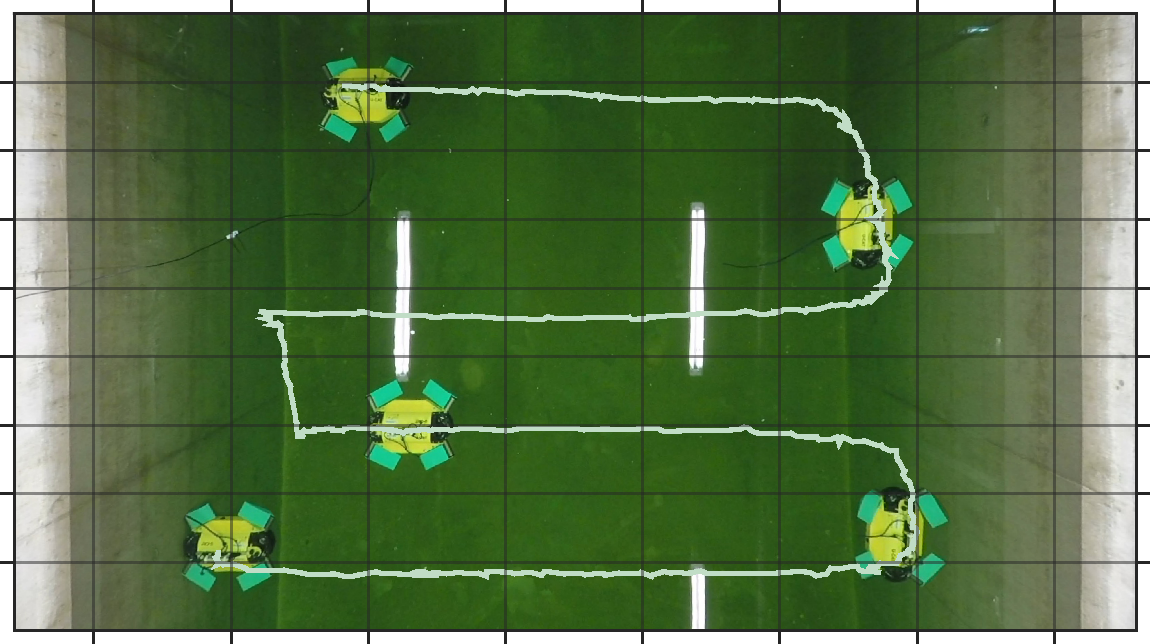
\includegraphics[width=3.0in]{img/autodepthyawtrajectory/autodepthyaw.pdf}
\caption{Lawnmower trajectory with automatic depth and yaw control.}
\label{autodepthyawtrajectory}
\end{figure}

\begin{figure} 
	\centering 
	% This file was created by matlab2tikz.
%
%The latest updates can be retrieved from
%  http://www.mathworks.com/matlabcentral/fileexchange/22022-matlab2tikz-matlab2tikz
%where you can also make suggestions and rate matlab2tikz.
%
\definecolor{mycolor1}{rgb}{0.00000,0.44700,0.74100}%
\definecolor{mycolor2}{rgb}{0.85000,0.32500,0.09800}%
%
\begin{tikzpicture}

\begin{axis}[%
width=2.75in,
height=1.288in,
at={(0.0in,1.7in)},
scale only axis,
xmin=0,
xmax=400,
ymin=-2,
ymax=0,
ylabel={Depth, m},
axis background/.style={fill=white},
axis x line*=bottom,
axis y line*=left,
legend style={legend cell align=left,align=left,draw=white!15!black}
]
\addplot [color=mycolor1,solid,line width=1.0pt]
  table[row sep=crcr]{%
0	0.0389701149285082\\
0.128567934036255	-0.20000098963997\\
0.23709774017334	-0.200007871459869\\
0.360261678695679	-0.200026365103805\\
0.477649688720703	-0.200062054197072\\
0.592426300048828	-0.200120287145641\\
0.713316679000854	-0.200325456856959\\
0.832791566848755	-0.200481731358592\\
0.947200775146484	-0.200680506205941\\
1.06371164321899	-0.200926253433284\\
1.17927694320679	-0.201223403927372\\
1.29525566101074	-0.201575926003605\\
1.42593836784363	-0.202465261211387\\
1.54359602928162	-0.203006354762173\\
1.66134524345398	-0.203619682660578\\
1.779372215271	-0.20430834067688\\
1.89714741706848	-0.205072464708389\\
2.0246057510376	-0.206847568966778\\
2.14394402503967	-0.20786270807072\\
2.25981140136719	-0.20897099850704\\
2.37606334686279	-0.210163421315184\\
2.49325108528137	-0.211453799845105\\
2.61397242546082	-0.214325819586877\\
2.7342324256897	-0.21591089757895\\
2.85399174690247	-0.217598816319597\\
2.9773223400116	-0.219390254239767\\
3.09894633293152	-0.221287886156852\\
3.22274589538574	-0.225410542886928\\
3.34044241905212	-0.227625690589505\\
3.46521592140198	-0.229964984516992\\
3.58432030677795	-0.232405832776582\\
3.70124936103821	-0.234963233664214\\
3.82879734039307	-0.240420793200836\\
3.94902539253235	-0.243328742481981\\
4.06559133529663	-0.246339120176606\\
4.18638062477112	-0.249468641778322\\
4.30978870391846	-0.256068273336291\\
4.43096494674683	-0.259545729329451\\
4.54643678665161	-0.263134989540704\\
4.66335535049438	-0.266840761240964\\
4.78018689155579	-0.270662009578926\\
4.89561343193054	-0.274597510978572\\
5.0122857093811	-0.282816201491742\\
5.13143873214722	-0.287084754784668\\
5.24802136421204	-0.291470934817573\\
5.36497807502747	-0.295968913162998\\
5.4817373752594	-0.300575369935521\\
5.59768128395081	-0.305290609097655\\
5.7228536605835	-0.315045132463209\\
5.84049129486084	-0.320080135893946\\
5.95813941955566	-0.325219110346956\\
6.07410430908203	-0.330461262100359\\
6.18973875045776	-0.33580136250298\\
6.31222772598267	-0.346782594915495\\
6.43212342262268	-0.352415539884771\\
6.55075764656067	-0.358146766673087\\
6.66790509223938	-0.363982449382007\\
6.78407430648804	-0.369875906020291\\
6.90550827980042	-0.375886356949542\\
7.02525424957275	-0.388134048859209\\
7.14335322380066	-0.394381651717842\\
7.25829005241394	-0.400715782021558\\
7.37526965141296	-0.4071212222087\\
7.49042367935181	-0.413606536568784\\
7.60975074768066	-0.426787520098878\\
7.72972798347473	-0.433480863048747\\
7.84631395339966	-0.440243437623834\\
7.96458697319031	-0.447069767869766\\
8.08108568191528	-0.453960618819192\\
8.20078325271606	-0.460883746035602\\
8.32510805130005	-0.474941336844307\\
8.44379997253418	-0.482025538070762\\
8.56049370765686	-0.489170043937726\\
8.68121767044067	-0.496357033671769\\
8.79648661613464	-0.503590462721994\\
8.92178440093994	-0.518160648037877\\
9.03781962394714	-0.52553479578371\\
9.15392589569092	-0.532863765563843\\
9.26878833770752	-0.540252811065896\\
9.3846070766449	-0.547666339634172\\
9.49978089332581	-0.555102120780801\\
9.6098964214325	-0.570045416990586\\
9.72643542289734	-0.577525405366898\\
9.84174728393555	-0.584997224321476\\
9.95688199996948	-0.592494106878612\\
10.0725867748261	-0.599996244907379\\
10.1896333694458	-0.607495935177885\\
10.3091700077057	-0.622483590651385\\
10.4297633171082	-0.629962087021077\\
10.5481922626495	-0.637465355820609\\
10.6677095890045	-0.644887405022285\\
10.7831606864929	-0.652326081950615\\
10.8992886543274	-0.659738891904178\\
11.0209383964539	-0.674495856762956\\
11.1361699104309	-0.681837676640707\\
11.255526304245	-0.68914089975142\\
11.3743257522583	-0.696405977165248\\
11.4902603626251	-0.703630419596599\\
11.6099076271057	-0.717962747405165\\
11.7273342609406	-0.725066183974862\\
11.8427584171295	-0.732107669295497\\
11.963127374649	-0.739103179044648\\
12.0805020332336	-0.746057854677784\\
12.1971468925476	-0.752961553443823\\
12.321063041687	-0.766532369363151\\
12.4353952407837	-0.773202538531976\\
12.5541729927063	-0.779829961048381\\
12.6693925857544	-0.786401173926776\\
12.7844910621643	-0.792870078769746\\
12.9003326892853	-0.799277413961055\\
13.0209143161774	-0.811860753666879\\
13.1372683048248	-0.818031053295375\\
13.2552366256714	-0.824114709165411\\
13.3714377880096	-0.830115461084312\\
13.4864346981049	-0.836026222217644\\
13.6021764278412	-0.841847285210791\\
13.7253313064575	-0.853209093023375\\
13.8421852588654	-0.858747917152962\\
13.9571614265442	-0.864188970122194\\
14.0719330310822	-0.869532441951857\\
14.1870710849762	-0.87479033144675\\
14.3034090995789	-0.87991127656785\\
14.4188785552979	-0.889877224700838\\
14.5263104438782	-0.894697108283885\\
14.635507106781	-0.899413004019812\\
14.7529065608978	-0.904021057649977\\
14.8712167739868	-0.908524860629923\\
14.9887986183167	-0.91290970037638\\
15.1137776374817	-0.921356149597544\\
15.2318382263184	-0.925395968819311\\
15.3530659675598	-0.929332368547835\\
15.4688670635223	-0.933152104893798\\
15.5916962623596	-0.93685906877657\\
15.7232716083527	-0.943926682062548\\
15.8452746868134	-0.947285782802114\\
15.9622750282288	-0.950532482922704\\
16.0805914402008	-0.953661626918754\\
16.1983213424683	-0.956675692188269\\
16.322568655014	-0.962362363921429\\
16.4397079944611	-0.965032185139649\\
16.5606436729431	-0.967590243227691\\
16.6780467033386	-0.970036274347744\\
16.7970895767212	-0.972370567768053\\
16.9203610420227	-0.976707748827516\\
17.0381717681885	-0.978708783757844\\
17.1586999893188	-0.980608074823177\\
17.2800252437592	-0.982399927057023\\
17.3985452651978	-0.984087791592523\\
17.5202536582947	-0.987156919606734\\
17.6395680904388	-0.988544397602672\\
17.7604587078094	-0.989834851017348\\
17.8811600208282	-0.991031815145079\\
17.9975564479828	-0.99213722118804\\
18.1220283508301	-0.994082212544068\\
18.2419939041138	-0.994926126674163\\
18.3622553348541	-0.995691860085212\\
18.4774153232574	-0.99637916582448\\
18.5924446582794	-0.996992799759352\\
18.7210695743561	-0.998011687983086\\
18.8420097827911	-0.998423808269735\\
18.9573149681091	-0.998777585762236\\
19.0720772743225	-0.999073490317193\\
19.1879496574402	-0.999319219041293\\
19.303564786911	-0.999518091020336\\
19.4223155975342	-0.999793467269336\\
19.5384032726288	-0.999879595913483\\
19.6533706188202	-0.999938012794257\\
19.7702083587646	-0.999973580689479\\
19.8845820426941	-0.999992109078596\\
20.0023400783539	-0.99999900549669\\
20.1240646839142	-1\\
20.2387833595276	-1\\
20.3550977706909	-1\\
20.4714040756226	-1\\
20.5891606807709	-1\\
20.7139387130737	-1\\
20.8337023258209	-1\\
20.9538297653198	-1\\
21.0712020397186	-1\\
21.1879312992096	-1\\
21.2968072891235	-1\\
21.417649269104	-1\\
21.5336463451386	-1\\
21.652916431427	-1\\
21.7742357254028	-1\\
21.9009032249451	-1\\
22.0224785804749	-1\\
22.1375954151154	-1\\
22.2547373771667	-1\\
22.3735589981079	-1\\
22.4923388957977	-1\\
22.6110966205597	-1\\
22.7283222675323	-1\\
22.8450126647949	-1\\
22.9612357616425	-1\\
23.0775172710419	-1\\
23.1942002773285	-1\\
23.312618970871	-1\\
23.4325699806213	-1\\
23.5487947463989	-1\\
23.6653835773468	-1\\
23.7822437286377	-1\\
23.899781703949	-1\\
24.0209267139435	-1\\
24.1436810493469	-1\\
24.2622315883636	-1\\
24.3789463043213	-1\\
24.4869904518127	-1\\
24.6076490879059	-1\\
24.72691822052	-1\\
24.8442454338074	-1\\
24.9636063575745	-1\\
25.0859262943268	-1\\
25.206689119339	-1\\
25.3256826400757	-1\\
25.4424843788147	-1\\
25.559556722641	-1\\
25.6766374111176	-1\\
25.7935810089111	-1\\
25.9142420291901	-1\\
26.0318152904511	-1\\
26.1471230983734	-1\\
26.2634162902832	-1\\
26.3805155754089	-1\\
26.498076915741	-1\\
26.6197485923767	-1\\
26.7376999855042	-1\\
26.8556926250458	-1\\
26.9734103679657	-1\\
27.10023188591	-1\\
27.2269637584686	-1\\
27.3456106185913	-1\\
27.4640703201294	-1\\
27.5824010372162	-1\\
27.6911146640778	-1\\
27.8120329380035	-1\\
27.92986536026	-1\\
28.0462920665741	-1\\
28.1657154560089	-1\\
28.2856180667877	-1\\
28.4060413837433	-1\\
28.5248494148254	-1\\
28.6426594257355	-1\\
28.7613134384155	-1\\
28.8809962272644	-1\\
28.9993555545807	-1\\
29.1208033561707	-1\\
29.2389667034149	-1\\
29.356175661087	-1\\
29.4716284275055	-1\\
29.5904290676117	-1\\
29.7115862369537	-1\\
29.8290646076202	-1\\
29.9480874538422	-1\\
30.0658869743347	-1\\
30.1820895671844	-1\\
30.3028457164764	-1\\
30.4296402931213	-1\\
30.5509314537048	-1\\
30.6696627140045	-1\\
30.7859964370728	-1\\
30.9124312400818	-1\\
31.0333435535431	-1\\
31.1521117687225	-1\\
31.2723202705383	-1\\
31.3921799659729	-1\\
31.5173916816711	-1\\
31.6330764293671	-1\\
31.7497973442078	-1\\
31.8683753013611	-1\\
31.9841461181641	-1\\
32.099663734436	-1\\
32.2208316326141	-1\\
32.3375272750854	-1\\
32.4537599086761	-1\\
32.5746433734894	-1\\
32.691121339798	-1\\
32.8212633132935	-1\\
32.9436891078949	-1\\
33.0607485771179	-1\\
33.178094625473	-1\\
33.2940533161163	-1\\
33.4147336483002	-1\\
33.5420446395874	-1\\
33.6586003303528	-1\\
33.7859563827515	-1\\
33.9107246398926	-1\\
34.0319883823395	-1\\
34.1516280174255	-1\\
34.2687339782715	-1\\
34.3885943889618	-1\\
34.510103225708	-1\\
34.6366753578186	-1\\
34.7567729949951	-1\\
34.8777062892914	-1\\
34.9941029548645	-1\\
35.1136519908905	-1\\
35.2321090698242	-1\\
35.3483109474182	-1\\
35.4655339717865	-1\\
35.579085111618	-1\\
35.6968936920166	-1\\
35.8171737194061	-1\\
35.9348783493042	-1\\
36.0523617267609	-1\\
36.1718957424164	-1\\
36.2903060913086	-1\\
36.4094586372375	-1\\
36.5279867649078	-1\\
36.6443829536438	-1\\
36.7649693489075	-1\\
36.8807199001312	-1\\
36.9970209598541	-1\\
37.1179893016815	-1\\
37.2400689125061	-1\\
37.3591990470886	-1\\
37.4799625873566	-1\\
37.6012346744537	-1\\
37.7268447875977	-1\\
37.845874786377	-1\\
37.9641432762146	-1\\
38.0900681018829	-1\\
38.2155983448029	-1\\
38.334591627121	-1\\
38.4413390159607	-1\\
38.5608673095703	-1\\
38.679413318634	-1\\
38.797168970108	-1\\
38.9208960533142	-1\\
39.0419497489929	-1\\
39.1599609851837	-1\\
39.2806394100189	-1\\
39.3975422382355	-1\\
39.5224359035492	-1\\
39.6538290977478	-1\\
39.7633957862854	-1\\
39.8898549079895	-1\\
40.0147824287415	-1\\
40.1387269496918	-1\\
40.2538642883301	-1\\
40.3714239597321	-1\\
40.4888899326324	-1\\
40.6108539104462	-1\\
40.7313766479492	-1\\
40.8465723991394	-1\\
40.9625110626221	-1\\
41.0785489082336	-1\\
41.19371509552	-1\\
41.3120539188385	-1\\
41.4294381141663	-1\\
41.5461759567261	-1\\
41.6609899997711	-1\\
41.7775459289551	-1\\
41.8932371139526	-1\\
42.0110926628113	-1\\
42.1296873092651	-1\\
42.2487809658051	-1\\
42.3690469264984	-1\\
42.4849536418915	-1\\
42.6028633117676	-1\\
42.7245817184448	-1\\
42.8456220626831	-1\\
42.9625976085663	-1\\
43.0878820419312	-1\\
43.2092730998993	-1\\
43.3290293216705	-1\\
43.4472336769104	-1\\
43.5623359680176	-1\\
43.6786210536957	-1\\
43.7985756397247	-1\\
43.9287989139557	-1\\
44.0362057685852	-1\\
44.154801607132	-1\\
44.2746860980988	-1\\
44.3947405815125	-1\\
44.5109965801239	-1\\
44.6291222572327	-1\\
44.7458493709564	-1\\
44.8670344352722	-1\\
44.9859220981598	-1\\
45.1079432964325	-1\\
45.2289938926697	-1\\
45.3473963737488	-1\\
45.4641089439392	-1\\
45.5863876342773	-1\\
45.7071306705475	-1\\
45.8267126083374	-1\\
45.9701249599457	-1\\
46.0856459140778	-1\\
46.2041110992432	-1\\
46.3254127502441	-1\\
46.4465720653534	-1\\
46.563939332962	-1\\
46.6832189559937	-1\\
46.8011174201965	-1\\
46.9237370491028	-1\\
47.038104057312	-1\\
47.1532740592957	-1\\
47.2732737064362	-1\\
47.3925280570984	-1\\
47.5141973495483	-1\\
47.6338739395142	-1\\
47.7516672611237	-1\\
47.869472026825	-1\\
47.988537311554	-1\\
48.1119470596313	-1\\
48.2333869934082	-1\\
48.3531329631805	-1\\
48.4732151031494	-1\\
48.5968573093414	-1\\
48.7265367507935	-1\\
48.8431167602539	-1\\
48.9595906734467	-1\\
49.0771200656891	-1\\
49.1948709487915	-1\\
49.3188617229462	-1\\
49.4377567768097	-1\\
49.5454430580139	-1\\
49.6526184082031	-1\\
49.761602640152	-1\\
49.8777506351471	-1\\
49.9964156150818	-1\\
50.1195020675659	-1\\
50.2376611232758	-1\\
50.3579256534576	-1\\
50.4754223823547	-1\\
50.5991365909576	-1\\
50.7259979248047	-1\\
50.8439955711365	-1\\
50.9647123813629	-1\\
51.0864520072937	-1\\
51.2121245861053	-1\\
51.3318793773651	-1\\
51.4518740177155	-1\\
51.5729455947876	-1\\
51.7029635906219	-1\\
51.8274130821228	-1\\
51.946218252182	-1\\
52.0648760795593	-1\\
52.1826047897339	-1\\
52.2990300655365	-1\\
52.4221529960632	-1\\
52.5393903255463	-1\\
52.6583023071289	-1\\
52.7754564285278	-1\\
52.8919582366943	-1\\
53.0150213241577	-1\\
53.1351716518402	-1\\
53.2527170181274	-1\\
53.370265007019	-1\\
53.4863042831421	-1\\
53.6023237705231	-1\\
53.726423740387	-1\\
53.8446946144104	-1\\
53.9602580070496	-1\\
54.0752177238464	-1\\
54.1918897628784	-1\\
54.3141095638275	-1\\
54.4329645633698	-1\\
54.5487444400787	-1\\
54.6720762252808	-1\\
54.7914290428162	-1\\
54.8997271060944	-1\\
55.0229687690735	-1\\
55.1414303779602	-1\\
55.2609295845032	-1\\
55.377852678299	-1\\
55.4967160224915	-1\\
55.6221296787262	-1\\
55.7441673278809	-1\\
55.8631706237793	-1\\
55.9808156490326	-1\\
56.0986320972443	-1\\
56.2194337844849	-1\\
56.3380644321442	-1\\
56.458281993866	-1\\
56.5769543647766	-1\\
56.698276758194	-1\\
56.8201999664307	-1\\
56.9411180019379	-1\\
57.0609641075134	-1\\
57.1807217597961	-1\\
57.3108339309692	-1\\
57.4337320327759	-1\\
57.5541479587555	-1\\
57.6726815700531	-1\\
57.7793490886688	-1\\
57.8945636749268	-1\\
58.0149185657501	-1\\
58.1323699951172	-1\\
58.2515914440155	-1\\
58.3702299594879	-1\\
58.4874963760376	-1\\
58.6130516529083	-1\\
58.7403733730316	-1\\
58.859180688858	-1\\
58.9801995754242	-1\\
59.0984704494476	-1\\
59.2219762802124	-1\\
59.3407797813416	-1\\
59.4631490707397	-1\\
59.5843353271484	-1\\
59.7100620269775	-1\\
59.8332905769348	-1\\
59.9528429508209	-1\\
60.0686156749725	-1\\
60.1883211135864	-1\\
60.29545378685	-1\\
60.4145810604095	-1\\
60.5418539047241	-1\\
60.6603026390076	-1\\
60.7770907878876	-1\\
60.8913662433624	-1\\
61.0132427215576	-1\\
61.1323204040527	-1\\
61.2505168914795	-1\\
61.368426322937	-1\\
61.4846336841583	-1\\
61.6015086174011	-1\\
61.7210116386414	-1\\
61.8429927825928	-1\\
61.9619777202606	-1\\
62.0813956260681	-1\\
62.1988279819489	-1\\
62.3209497928619	-1\\
62.438188791275	-1\\
62.5559771060944	-1\\
62.6751494407654	-1\\
62.7945806980133	-1\\
62.9147894382477	-1\\
63.0441184043884	-1\\
63.1614112854004	-1\\
63.2860209941864	-1\\
63.4048306941986	-1\\
63.5248489379883	-1\\
63.6492249965668	-1\\
63.7773785591125	-1\\
63.8987736701965	-1\\
64.0232672691345	-1\\
64.1512815952301	-1\\
64.2747156620026	-1\\
64.3943839073181	-1\\
64.5146837234497	-1\\
64.6391599178314	-1\\
64.7555365562439	-1\\
64.8750603199005	-1\\
64.9950664043427	-1\\
65.1205313205719	-1\\
65.2467226982117	-1\\
65.3632986545563	-1\\
65.4800024032593	-1\\
65.5976052284241	-1\\
65.7185900211334	-1\\
65.8364410400391	-1\\
65.9528126716614	-1\\
66.069060087204	-1\\
66.1849191188812	-1\\
66.3015604019165	-1\\
66.4265587329865	-1\\
66.5408203601837	-1\\
66.6576170921326	-1\\
66.7789273262024	-1\\
66.8955924510956	-1\\
67.0304770469666	-1\\
67.1468102931976	-1\\
67.2641055583954	-1\\
67.3819849491119	-1\\
67.4990980625153	-1\\
67.6252243518829	-1\\
67.7434310913086	-1\\
67.8611330986023	-1\\
67.9789526462555	-1\\
68.0952293872833	-1\\
68.2176086902618	-1\\
68.334903717041	-1\\
68.4511060714722	-1\\
68.5676560401917	-1\\
68.6841170787811	-1\\
68.8006446361542	-1\\
68.9222979545593	-1\\
69.0390865802765	-1\\
69.1548728942871	-1\\
69.271146774292	-1\\
69.3903856277466	-1\\
69.4982120990753	-1\\
69.6241700649261	-1\\
69.7416253089905	-1\\
69.8584797382355	-1\\
69.9759140014648	-1\\
70.1006820201874	-1\\
70.2326719760895	-1\\
70.3497257232666	-1\\
70.4658913612366	-1\\
70.5829770565033	-1\\
70.6985011100769	-1\\
70.8204445838928	-1\\
70.935683965683	-1\\
71.0521423816681	-1\\
71.1688859462738	-1\\
71.2859237194061	-1\\
71.4038016796112	-1\\
71.5277004241943	-1\\
71.6445684432983	-1\\
71.7602927684784	-1\\
71.8760499954224	-1\\
71.9933040142059	-1\\
72.1123614311218	-1\\
72.2302219867706	-1\\
72.3469839096069	-1\\
72.4698903560638	-1\\
72.5854756832123	-1\\
72.7008640766144	-1\\
72.8110716342926	-1\\
72.9445219039917	-1\\
73.0629687309265	-1\\
73.1830003261566	-1\\
73.3008270263672	-1\\
73.4271891117096	-1\\
73.5438380241394	-1\\
73.6599402427673	-1\\
73.7773914337158	-1\\
73.8950803279877	-1\\
74.0257155895233	-1\\
74.1461434364319	-1\\
74.2630655765533	-1\\
74.379775762558	-1\\
74.4964563846588	-1\\
74.6196303367615	-1\\
74.7372705936432	-1\\
74.8554470539093	-1\\
74.9739079475403	-1\\
75.0952033996582	-1\\
75.2260119915009	-1\\
75.3416826725006	-1\\
75.4652903079987	-1\\
75.584287405014	-1\\
75.7015631198883	-1\\
75.8279469013214	-1\\
75.9501624107361	-1\\
76.0681176185608	-1\\
76.185400724411	-1\\
76.3028497695923	-1\\
76.4230129718781	-1\\
76.5389676094055	-1\\
76.6562759876251	-1\\
76.7723259925842	-1\\
76.887264251709	-1\\
77.0084927082062	-1\\
77.1297652721405	-1\\
77.2480657100677	-1\\
77.3655200004578	-1\\
77.4827656745911	-1\\
77.5993065834045	-1\\
77.7229557037354	-1\\
77.8409907817841	-1\\
77.9583625793457	-1\\
78.0762536525726	-1\\
78.19580078125	-1\\
78.3261294364929	-1\\
78.4409565925598	-1\\
78.5572400093079	-1\\
78.6727719306946	-1\\
78.7904622554779	-1\\
78.9131140708923	-1\\
79.0313346385956	-1\\
79.1468932628632	-1\\
79.2663886547089	-1\\
79.3838341236115	-1\\
79.4996984004974	-1\\
79.6236484050751	-1\\
79.7440972328186	-1\\
79.863365650177	-1\\
79.9814684391022	-1\\
80.0961365699768	-1\\
80.219957113266	-1\\
80.3349583148956	-1\\
80.4502766132355	-1\\
80.5661532878876	-1\\
80.6817469596863	-1\\
80.7961423397064	-1\\
80.9197342395782	-1\\
81.0349442958832	-1\\
81.1508612632751	-1\\
81.2670390605927	-1\\
81.3834314346313	-1\\
81.500949382782	-1\\
81.6276485919952	-1\\
81.7437567710876	-1\\
81.8569459915161	-1\\
81.9734296798706	-1\\
82.0891983509064	-1\\
82.2120349407196	-1\\
82.3329937458038	-1\\
82.4523253440857	-1\\
82.571831703186	-1\\
82.6892063617706	-1\\
82.8231933116913	-1\\
82.9412219524384	-1\\
83.0599200725555	-1\\
83.1813879013062	-1\\
83.3019089698792	-1\\
83.4263334274292	-1\\
83.5440254211426	-1\\
83.6626126766205	-1\\
83.7817199230194	-1\\
83.8977620601654	-1\\
84.0194959640503	-1\\
84.1379399299622	-1\\
84.255640745163	-1\\
84.3737421035767	-1\\
84.4939334392548	-1\\
84.6204285621643	-1\\
84.7461416721344	-1\\
84.8624653816223	-1\\
84.9805903434753	-1\\
85.0991003513336	-1\\
85.2282874584198	-1\\
85.3439745903015	-1\\
85.4605510234833	-1\\
85.5785663127899	-1\\
85.6955261230469	-1\\
85.8163685798645	-1\\
85.9342648983002	-1\\
86.0495002269745	-1\\
86.1703014373779	-1\\
86.2891452312469	-1\\
86.4133095741272	-1\\
86.5354599952698	-1\\
86.6558544635773	-1\\
86.7723960876465	-1\\
86.8887124061584	-1\\
87.0071432590485	-1\\
87.1281878948212	-1\\
87.2467379570007	-1\\
87.3769564628601	-1\\
87.4949579238892	-1\\
87.6218631267548	-1\\
87.739305973053	-1\\
87.8546977043152	-1\\
87.962162733078	-1\\
88.0787789821625	-1\\
88.1957154273987	-1\\
88.3259830474854	-1\\
88.4426538944244	-1\\
88.5607891082764	-1\\
88.676308631897	-1\\
88.7938899993896	-1\\
88.9120676517487	-1\\
89.031543970108	-1\\
89.1493933200836	-1\\
89.2681424617767	-1\\
89.3882019519806	-1\\
89.5085854530334	-1\\
89.642322063446	-1\\
89.7620453834534	-1\\
89.8798253536224	-1\\
89.9991500377655	-1\\
90.123767375946	-1\\
90.2410581111908	-1\\
90.3600914478302	-1\\
90.4805912971497	-1\\
90.603483915329	-1\\
90.7317852973938	-1\\
90.8386993408203	-1\\
90.9557363986969	-1\\
91.0745782852173	-1\\
91.1928079128265	-1\\
91.3233835697174	-1\\
91.4493141174316	-1\\
91.5674860477448	-1\\
91.6875517368317	-1\\
91.8102684020996	-1\\
91.9298567771912	-1\\
92.0477304458618	-1\\
92.1658201217651	-1\\
92.2827899456024	-1\\
92.3997087478638	-1\\
92.523916721344	-1\\
92.643171787262	-1\\
92.7609190940857	-1\\
92.8827590942383	-1\\
93.0043525695801	-1\\
93.1283533573151	-1\\
93.2511520385742	-1\\
93.3671822547913	-1\\
93.48606300354	-1\\
93.6075870990753	-1\\
93.7193522453308	-1\\
93.8370764255524	-1\\
93.9596326351166	-1\\
94.0778028964996	-1\\
94.1960380077362	-1\\
94.3196880817413	-1\\
94.438095331192	-1\\
94.5557656288147	-1\\
94.6746792793274	-1\\
94.7951686382294	-1\\
94.917820930481	-1\\
95.0371203422546	-1\\
95.1566500663757	-1\\
95.2787001132965	-1\\
95.4044089317322	-1\\
95.5296950340271	-1\\
95.6514916419983	-1\\
95.7737944126129	-1\\
95.8931484222412	-1\\
96.0124952793121	-1\\
96.1390240192413	-1\\
96.2548532485962	-1\\
96.3724362850189	-1\\
96.4929559230804	-1\\
96.6201963424683	-1\\
96.7377350330353	-1\\
96.8576922416687	-1\\
96.9808750152588	-1\\
97.0975987911224	-1\\
97.2166197299957	-1\\
97.3345267772675	-1\\
97.4630613327026	-1\\
97.5799245834351	-1\\
97.6947491168976	-1\\
97.817507982254	-1\\
97.9336366653442	-1\\
98.0497460365295	-1\\
98.1680107116699	-1\\
98.285923242569	-1\\
98.410920381546	-1\\
98.5432286262512	-1\\
98.6599414348602	-1\\
98.783087015152	-1\\
98.9067656993866	-1\\
99.0291924476624	-1\\
99.1446526050568	-1\\
99.2604501247406	-1\\
99.3790180683136	-1\\
99.4938876628876	-1\\
99.6131086349487	-1\\
99.7472250461578	-1\\
99.8642942905426	-1\\
99.9812269210815	-1\\
100.097516059875	-1\\
100.216782569885	-1\\
100.332570791245	-1\\
100.447907686234	-1\\
100.565411567688	-1\\
100.684621572495	-1\\
100.802045345306	-1\\
100.923404932022	-1\\
101.040811300278	-1\\
101.157584905624	-1\\
101.276284694672	-1\\
101.397715330124	-1\\
101.515685796738	-1\\
101.63976764679	-1\\
101.758883237839	-1\\
101.880798339844	-1\\
101.997114419937	-1\\
102.11830663681	-1\\
102.235694408417	-1\\
102.356562614441	-1\\
102.47599363327	-1\\
102.591747045517	-1\\
102.712530612946	-1\\
102.846260786057	-1\\
102.96533703804	-1\\
103.086997270584	-1\\
103.202850341797	-1\\
103.328033924103	-1\\
103.449868917465	-1\\
103.571708679199	-1\\
103.693840026855	-1\\
103.814652681351	-1\\
103.933022260666	-1\\
104.04950094223	-1\\
104.173677921295	-1\\
104.291888952255	-1\\
104.41172170639	-1\\
104.532433986664	-1\\
104.649629116058	-1\\
104.766284942627	-1\\
104.874203920364	-1\\
104.988668441772	-1\\
105.108634233475	-1\\
105.233217954636	-1\\
105.352010011673	-1\\
105.473834991455	-1\\
105.592943668365	-1\\
105.721731901169	-1\\
105.842823982239	-1\\
105.96800994873	-1\\
106.084530353546	-1\\
106.200856685638	-1\\
106.326443433762	-1\\
106.447603702545	-1\\
106.569824934006	-1\\
106.688117742538	-1\\
106.808583021164	-1\\
106.929294109344	-1\\
107.047634124756	-1\\
107.167046308517	-1\\
107.285158634186	-1\\
107.406668901443	-1\\
107.524631261826	-1\\
107.652327299118	-1\\
107.771854400635	-1\\
107.892526626587	-1\\
108.018727779388	-1\\
108.139483451843	-1\\
108.275796413422	-1\\
108.408117771149	-1\\
108.52952837944	-1\\
108.646874666214	-1\\
108.778008460999	-1\\
108.895855426788	-1\\
109.020056724548	-1\\
109.137973308563	-1\\
109.259709119797	-1\\
109.377588748932	-1\\
109.494613647461	-1\\
109.614352941513	-1\\
109.734014987946	-1\\
109.85042142868	-1\\
109.966882228851	-1\\
110.082812786102	-1\\
110.199594736099	-1\\
110.320652961731	-1\\
110.439800024033	-1\\
110.557643413544	-1\\
110.674001693726	-1\\
110.791682720184	-1\\
110.916194915771	-1\\
111.039717674255	-1\\
111.160708665848	-1\\
111.278521776199	-1\\
111.394064426422	-1\\
111.52529001236	-1\\
111.642690896988	-1\\
111.761339426041	-1\\
111.88135433197	-1\\
111.998483657837	-1\\
112.126853466034	-1\\
112.235118627548	-1\\
112.353248596191	-1\\
112.469237565994	-1\\
112.58568072319	-1\\
112.700716018677	-1\\
112.825221776962	-1\\
112.944623231888	-1\\
113.062089681625	-1\\
113.179521799088	-1\\
113.297884464264	-1\\
113.421987295151	-1\\
113.539239645004	-1\\
113.655106306076	-1\\
113.773491382599	-1\\
113.889837026596	-1\\
114.009506464005	-1\\
114.127437591553	-1\\
114.243179798126	-1\\
114.371032953262	-1\\
114.485771656036	-1\\
114.602652311325	-1\\
114.711500406265	-1\\
114.83279132843	-1\\
114.950726985931	-1\\
115.068068027496	-1\\
115.1831407547	-1\\
115.304974794388	-1\\
115.42285323143	-1\\
115.541287899017	-1\\
115.658341646194	-1\\
115.777810096741	-1\\
115.897246599197	-1\\
116.020336389542	-1\\
116.138033628464	-1\\
116.256375074387	-1\\
116.373963356018	-1\\
116.491272687912	-1\\
116.613577365875	-1\\
116.733052253723	-1\\
116.849244356155	-1\\
116.964908599854	-1\\
117.080657243729	-1\\
117.199694395065	-1\\
117.328425645828	-1\\
117.454538106918	-1\\
117.572884082794	-1\\
117.694515943527	-1\\
117.818612098694	-1\\
117.937942028046	-1\\
118.054818630219	-1\\
118.172199010849	-1\\
118.292516231537	-1\\
118.417381048203	-1\\
118.534146308899	-1\\
118.65110206604	-1\\
118.768229961395	-1\\
118.885481595993	-1\\
119.007261276245	-1\\
119.128208398819	-1\\
119.245971441269	-1\\
119.368639945984	-1\\
119.485461235046	-1\\
119.60542845726	-1\\
119.727478981018	-1\\
119.845831394196	-1\\
119.965995788574	-1\\
120.086017608643	-1\\
120.218087434769	-1\\
120.335397005081	-1\\
120.455089330673	-1\\
120.57489490509	-1\\
120.701858043671	-1\\
120.828053236008	-1\\
120.948029756546	-1\\
121.067396402359	-1\\
121.185428380966	-1\\
121.308086395264	-1\\
121.429988622665	-1\\
121.548601388931	-1\\
121.666359901428	-1\\
121.784008979797	-1\\
121.902538299561	-1\\
122.024430751801	-1\\
122.142992973328	-1\\
122.260706663132	-1\\
122.377043962479	-1\\
122.493236780167	-1\\
122.613568305969	-1\\
122.734192371368	-1\\
122.854323625565	-1\\
122.974060058594	-1\\
123.094359636307	-1\\
123.215411901474	-1\\
123.343360900879	-1\\
123.467113733292	-1\\
123.589666604996	-1\\
123.718051433563	-1\\
123.839378595352	-1\\
123.960837125778	-1\\
124.077944755554	-1\\
124.201848983765	-1\\
124.323084354401	-1\\
124.440416574478	-1\\
124.558483362198	-1\\
124.675290107727	-1\\
124.792513370514	-1\\
124.912897586823	-1\\
125.034992694855	-1\\
125.152811288834	-1\\
125.268517971039	-1\\
125.386526107788	-1\\
125.510220766068	-1\\
125.63085103035	-1\\
125.748598337173	-1\\
125.863663673401	-1\\
125.982511997223	-1\\
126.098521232605	-1\\
126.221908092499	-1\\
126.342790603638	-1\\
126.459090709686	-1\\
126.574915409088	-1\\
126.690464258194	-1\\
126.813173055649	-1\\
126.935035943985	-1\\
127.05372095108	-1\\
127.173546791077	-1\\
127.292256116867	-1\\
127.410692453384	-1\\
127.533827781677	-1\\
127.655178308487	-1\\
127.773284912109	-1\\
127.892408370972	-1\\
128.013930082321	-1\\
128.130841732025	-1\\
128.247958898544	-1\\
128.366129636765	-1\\
128.487149715424	-1\\
128.602142095566	-1\\
128.72753572464	-1\\
128.853795051575	-1\\
128.969651937485	-1\\
129.085394620895	-1\\
129.200865268707	-1\\
129.334604978561	-1\\
129.453157901764	-1\\
129.5716817379	-1\\
129.689053058624	-1\\
129.815322399139	-1\\
129.941370010376	-1\\
130.057779312134	-1\\
130.178614377975	-1\\
130.296676397324	-1\\
130.41955113411	-1\\
130.544739246368	-1\\
130.672749757767	-1\\
130.796020030975	-1\\
130.920007705688	-1\\
131.039919614792	-1\\
131.161774396896	-1\\
131.278342723846	-1\\
131.395566940308	-1\\
131.517250299454	-1\\
131.636354446411	-1\\
131.755297660828	-1\\
131.875865697861	-1\\
131.995578765869	-1\\
132.120656967163	-1\\
132.237110376358	-1\\
132.360620975494	-1\\
132.47687458992	-1\\
132.591871261597	-1\\
132.714523077011	-1\\
132.837373018265	-1\\
132.95308804512	-1\\
133.070163726807	-1\\
133.189285039902	-1\\
133.299071311951	-1\\
133.416173934937	-1\\
133.537395000458	-1\\
133.655927658081	-1\\
133.775428295136	-1\\
133.890897989273	-1\\
134.011530637741	-1\\
134.137135267258	-1\\
134.253814458847	-1\\
134.372984647751	-1\\
134.490713596344	-1\\
134.613069057465	-1\\
134.734668970108	-1\\
134.850907802582	-1\\
134.968181610107	-1\\
135.092602968216	-1\\
135.220740318298	-1\\
135.34071969986	-1\\
135.461559057236	-1\\
135.580070257187	-1\\
135.697991132736	-1\\
135.825088262558	-1\\
135.952345609665	-1\\
136.061336994171	-1\\
136.169261693954	-1\\
136.279601573944	-1\\
136.398263692856	-1\\
136.526332616806	-1\\
136.646062374115	-1\\
136.766164064407	-1\\
136.884125709534	-1\\
137.003291368485	-1\\
137.127099275589	-1\\
137.245801925659	-1\\
137.378331899643	-1\\
137.496576070786	-1\\
137.61821269989	-1\\
137.734758377075	-1\\
137.851808786392	-1\\
137.969990730286	-1\\
138.090230703354	-1\\
138.208931684494	-1\\
138.331170797348	-1\\
138.450174570084	-1\\
138.558357954025	-1\\
138.684016466141	-1\\
138.803205966949	-1\\
138.931487083435	-1\\
139.053814649582	-1\\
139.177795648575	-1\\
139.298140048981	-1\\
139.41933631897	-1\\
139.536660909653	-1\\
139.652044057846	-1\\
139.774836301804	-1\\
139.893887042999	-1\\
140.018599033356	-1\\
140.139780044556	-1\\
140.25800037384	-1\\
140.378381729126	-1\\
140.496215105057	-1\\
140.619688987732	-1\\
140.736233234406	-1\\
140.852953672409	-1\\
140.969975948334	-1\\
141.08827495575	-1\\
141.211177349091	-1\\
141.330662727356	-1\\
141.448151350021	-1\\
141.56573843956	-1\\
141.685802936554	-1\\
141.793720006943	-1\\
141.926943778992	-1\\
142.038487434387	-1\\
142.155391454697	-1\\
142.271776914597	-1\\
142.388154268265	-1\\
142.505457639694	-1\\
142.629267930985	-1\\
142.747956991196	-1\\
142.869057655334	-1\\
142.989644050598	-1\\
143.114429950714	-1\\
143.234024047852	-1\\
143.351624965668	-1\\
143.472202777863	-1\\
143.591844320297	-1\\
143.715491771698	-1\\
143.835176706314	-1\\
143.952630281448	-1\\
144.071766614914	-1\\
144.190641641617	-1\\
144.312726259232	-1\\
144.431756734848	-1\\
144.549063920975	-1\\
144.665835618973	-1\\
144.775270700455	-1\\
144.89245891571	-1\\
145.017548322678	-1\\
145.135432720184	-1\\
145.256297111511	-1\\
145.374266386032	-1\\
145.492367267609	-1\\
145.612869739532	-1\\
145.730382442474	-1\\
145.849091053009	-1\\
145.965609788895	-1\\
146.081219673157	-1\\
146.198352336884	-1\\
146.323606014252	-1\\
146.450052022934	-1\\
146.581218957901	-1\\
146.702919721603	-1\\
146.825583934784	-1\\
146.94512629509	-1\\
147.061172962189	-1\\
147.178787946701	-1\\
147.297563076019	-1\\
147.422853469849	-1\\
147.539096593857	-1\\
147.65834403038	-1\\
147.776300430298	-1\\
147.892101764679	-1\\
148.012923717499	-1\\
148.132328748703	-1\\
148.249218940735	-1\\
148.37232375145	-1\\
148.493239402771	-1\\
148.620643615723	-1\\
148.739820718765	-1\\
148.857184410095	-1\\
148.97669005394	-1\\
149.093281745911	-1\\
149.217266082764	-1\\
149.335099697113	-1\\
149.455506324768	-1\\
149.577174901962	-1\\
149.695862770081	-1\\
149.820860385895	-1\\
149.937474727631	-1\\
150.056907653809	-1\\
150.176924943924	-1\\
150.298782348633	-1\\
150.422783136368	-1\\
150.543019294739	-1\\
150.664403676987	-1\\
150.783126354218	-1\\
150.907816410065	-1\\
151.029525995255	-1\\
151.147881984711	-1\\
151.266986608505	-1\\
151.384665250778	-1\\
151.509589910507	-1\\
151.63161945343	-1\\
151.747914791107	-1\\
151.865430355072	-1\\
151.983963727951	-1\\
152.103866577148	-1\\
152.225573301315	-1\\
152.341715097427	-1\\
152.458237409592	-1\\
152.579072713852	-1\\
152.697747468948	-1\\
152.820305347443	-1\\
152.937455415726	-1\\
153.056965589523	-1\\
153.177596092224	-1\\
153.297831296921	-1\\
153.4217877388	-1\\
153.541974782944	-1\\
153.659811258316	-1\\
153.780398368835	-1\\
153.898724079132	-1\\
154.030678987503	-1\\
154.149399757385	-1\\
154.268062591553	-1\\
154.387421131134	-1\\
154.508031606674	-1\\
154.629028081894	-1\\
154.755628585815	-1\\
154.873702049255	-1\\
154.988698959351	-1\\
155.106095314026	-1\\
155.223120450974	-1\\
155.337862730026	-1\\
155.452651262283	-1\\
155.568437099457	-1\\
155.682864665985	-1\\
155.799315452576	-1\\
155.925179958344	-1\\
156.040384292603	-1\\
156.156295061111	-1\\
156.273215770721	-1\\
156.389993667603	-1\\
156.521359920502	-1\\
156.643590450287	-1\\
156.760227441788	-1\\
156.875767469406	-1\\
156.994802713394	-1\\
157.105027914047	-1\\
157.222836971283	-1\\
157.331174373627	-1\\
157.445703744888	-1\\
157.561136960983	-1\\
157.676664352417	-1\\
157.792426109314	-1\\
157.910400629044	-1\\
158.028652906418	-1\\
158.145127058029	-1\\
158.263221025467	-1\\
158.379386663437	-1\\
158.500216722488	-1\\
158.6225669384	-1\\
158.741764068604	-1\\
158.861213684082	-1\\
158.980214357376	-1\\
159.097261667252	-1\\
159.218347072601	-1\\
159.334944009781	-1\\
159.45743227005	-1\\
159.578087568283	-1\\
159.697711706162	-1\\
159.820204019547	-1\\
159.936640024185	-1\\
160.056360721588	-1\\
160.173850059509	-1\\
160.292071342468	-1\\
160.411796569824	-1\\
160.536797761917	-1\\
160.657581329346	-1\\
160.775665044785	-1\\
160.898665428162	-1\\
161.023272275925	-1\\
161.14275932312	-1\\
161.260900974274	-1\\
161.380721330643	-1\\
161.496388912201	-1\\
161.618421077728	-1\\
161.738621234894	-1\\
161.858696937561	-1\\
161.978631258011	-1\\
162.095179319382	-1\\
162.217166423798	-1\\
162.333594083786	-1\\
162.450327396393	-1\\
162.569973945618	-1\\
162.689110040665	-1\\
162.821834087372	-1\\
162.931188344955	-1\\
163.052484035492	-1\\
163.172482013702	-1\\
163.293699979782	-1\\
163.418110609055	-1\\
163.534255981445	-1\\
163.650656461716	-1\\
163.769585609436	-1\\
163.887135744095	-1\\
164.00835609436	-1\\
164.131262779236	-1\\
164.252358913422	-1\\
164.374146461487	-1\\
164.494735002518	-1\\
164.628165006638	-1\\
164.753010034561	-1\\
164.876163005829	-1\\
164.994390726089	-1\\
165.114107608795	-1\\
165.232831954956	-1\\
165.351297616959	-1\\
165.468116998672	-1\\
165.584056377411	-1\\
165.700635910034	-1\\
165.821511268616	-1\\
165.940846681595	-1\\
166.057680130005	-1\\
166.175805091858	-1\\
166.284489393234	-1\\
166.400059700012	-1\\
166.521265268326	-1\\
166.637959003448	-1\\
166.757736682892	-1\\
166.879140377045	-1\\
166.997625350952	-1\\
167.121918439865	-1\\
167.240861415863	-1\\
167.362046718597	-1\\
167.483603000641	-1\\
167.598207950592	-1\\
167.72117805481	-1\\
167.843032360077	-1\\
167.962278366089	-1\\
168.085710763931	-1\\
168.205646276474	-1\\
168.325225114822	-1\\
168.443657398224	-1\\
168.559341669083	-1\\
168.677160024643	-1\\
168.792711257935	-1\\
168.915741682053	-1\\
169.021066427231	-1\\
169.13566493988	-1\\
169.251564741135	-1\\
169.369535923004	-1\\
169.484881639481	-1\\
169.600671768188	-1\\
169.721211671829	-1\\
169.837479114532	-1\\
169.95262169838	-1\\
170.06938290596	-1\\
170.185239315033	-1\\
170.300663709641	-1\\
170.424835920334	-1\\
170.540788650513	-1\\
170.661809921265	-1\\
170.780440807343	-1\\
170.896418333054	-1\\
171.015513420105	-1\\
171.134831428528	-1\\
171.250607013702	-1\\
171.368449687958	-1\\
171.489287614822	-1\\
171.608593463898	-1\\
171.732382774353	-1\\
171.854763269424	-1\\
171.972273588181	-1\\
172.087949037552	-1\\
172.1998462677	-1\\
172.322540283203	-1\\
172.441299676895	-1\\
172.559248685837	-1\\
172.677491426468	-1\\
172.798320770264	-1\\
172.920937776566	-1\\
173.036880970001	-1\\
173.152084589005	-1\\
173.278311252594	-1\\
173.396414279938	-1\\
173.519567012787	-1\\
173.636456251144	-1\\
173.75328707695	-1\\
173.873244285584	-1\\
173.991289138794	-1\\
174.111161470413	-1\\
174.231019973755	-1\\
174.34862446785	-1\\
174.468298912048	-1\\
174.586971759796	-1\\
174.707680940628	-1\\
174.828310966492	-1\\
174.947741985321	-1\\
175.07018494606	-1\\
175.190100669861	-1\\
175.308684587479	-1\\
175.42767906189	-1\\
175.545337677002	-1\\
175.661831140518	-1\\
175.780704021454	-1\\
175.899207115173	-1\\
176.020544290543	-1\\
176.138382434845	-1\\
176.257276773453	-1\\
176.376409053802	-1\\
176.493320703506	-1\\
176.614426612854	-1\\
176.733111381531	-1\\
176.849702596664	-1\\
176.965839385986	-1\\
177.084892988205	-1\\
177.210205316544	-1\\
177.335043907166	-1\\
177.458210706711	-1\\
177.578722238541	-1\\
177.69893860817	-1\\
177.810732603073	-1\\
177.929997682571	-1\\
178.045988798141	-1\\
178.160966396332	-1\\
178.278456449509	-1\\
178.393887758255	-1\\
178.511774778366	-1\\
178.629238128662	-1\\
178.74649810791	-1\\
178.862468242645	-1\\
178.978127241135	-1\\
179.093883752823	-1\\
179.214411258698	-1\\
179.337694406509	-1\\
179.460665464401	-1\\
179.580244779587	-1\\
179.697244644165	-1\\
179.819692611694	-1\\
179.936594963074	-1\\
180.05695772171	-1\\
180.172463655472	-1\\
180.294500350952	-1\\
180.418352365494	-1\\
180.536638975143	-1\\
180.657129049301	-1\\
180.773898124695	-1\\
180.895420312881	-1\\
181.018888950348	-1\\
181.135719060898	-1\\
181.258190393448	-1\\
181.380466938019	-1\\
181.498796463013	-1\\
181.619323968887	-1\\
181.736752033234	-1\\
181.854254245758	-1\\
181.974356412888	-1\\
182.091675043106	-1\\
182.210711717606	-1\\
182.330718755722	-1\\
182.451153039932	-1\\
182.573118448257	-1\\
182.695859670639	-1\\
182.825438261032	-1\\
182.94762468338	-1\\
183.065774917603	-1\\
183.183116436005	-1\\
183.311310052872	-1\\
183.430938720703	-1\\
183.549381256104	-1\\
183.668886423111	-1\\
183.795167922974	-1\\
183.925498962402	-1\\
184.046275138855	-1\\
184.171757459641	-1\\
184.288804292679	-1\\
184.407275915146	-1\\
184.524176359177	-1\\
184.642269134521	-1\\
184.764863729477	-1\\
184.884906291962	-1\\
185.002422571182	-1\\
185.12166762352	-1\\
185.238850593567	-1\\
185.358242273331	-1\\
185.475007295609	-1\\
185.591399669647	-1\\
185.71271944046	-1\\
185.831021785736	-1\\
185.948975324631	-1\\
186.072809934616	-1\\
186.191916942596	-1\\
186.30765414238	-1\\
186.425024271011	-1\\
186.543176651001	-1\\
186.663460731506	-1\\
186.781717777252	-1\\
186.902823448181	-1\\
187.027881622314	-1\\
187.148216247559	-1\\
187.262766361237	-1\\
187.383119106293	-1\\
187.501223325729	-1\\
187.624304056168	-1\\
187.74147105217	-1\\
187.858792304993	-1\\
187.976943969727	-1\\
188.092515468597	-1\\
188.212659358978	-1\\
188.331575393677	-1\\
188.448595046997	-1\\
188.565117120743	-1\\
188.683941364288	-1\\
188.807558298111	-1\\
188.926686048508	-1\\
189.04275560379	-1\\
189.166485309601	-1\\
189.285697937012	-1\\
189.409625291824	-1\\
189.527344703674	-1\\
189.649236917496	-1\\
189.76667714119	-1\\
189.886167764664	-1\\
189.994468688965	-1\\
190.113757610321	-1\\
190.231609106064	-1\\
190.347747325897	-1\\
190.462718963623	-1\\
190.578649997711	-1\\
190.694207668304	-1\\
190.813088655472	-1\\
190.935091972351	-1\\
191.054718971252	-1\\
191.174164056778	-1\\
191.292766332626	-1\\
191.414224386215	-1\\
191.538759946823	-1\\
191.658549070358	-1\\
191.777737140656	-1\\
191.898719787598	-1\\
192.022958040237	-1\\
192.140654802322	-1\\
192.257327318192	-1\\
192.376019001007	-1\\
192.494312763214	-1\\
192.621449947357	-1\\
192.745119571686	-1\\
192.862479686737	-1\\
192.982965707779	-1\\
193.106468439102	-1\\
193.235753774643	-1\\
193.351061344147	-1\\
193.466830968857	-1\\
193.582957029343	-1\\
193.69880437851	-1\\
193.819038629532	-1\\
193.935678243637	-1\\
194.0522377491	-1\\
194.169019937515	-1\\
194.284527301788	-1\\
194.402375936508	-1\\
194.52364563942	-1\\
194.642249584198	-1\\
194.759013414383	-1\\
194.877747774124	-1\\
194.992896080017	-1\\
195.120820999146	-1\\
195.241200447083	-1\\
195.362151384354	-1\\
195.484598636627	-1\\
195.611095428467	-1\\
195.7321600914	-1\\
195.850021123886	-1\\
195.968133926392	-1\\
196.084402084351	-1\\
196.202898263931	-1\\
196.323963403702	-1\\
196.440827131271	-1\\
196.558548688889	-1\\
196.67561006546	-1\\
196.791358470917	-1\\
196.91805267334	-1\\
197.038358449936	-1\\
197.155007600784	-1\\
197.270785808563	-1\\
197.388625383377	-1\\
197.506351470947	-1\\
197.626836299896	-1\\
197.742875576019	-1\\
197.860193967819	-1\\
197.981253385544	-1\\
198.099961996078	-1\\
198.228233575821	-1\\
198.347423791885	-1\\
198.465114593506	-1\\
198.581954717636	-1\\
198.700736999512	-1\\
198.823775291443	-1\\
198.942129135132	-1\\
199.059656143188	-1\\
199.179266691208	-1\\
199.29604101181	-1\\
199.418354272842	-1\\
199.536884069443	-1\\
199.658656597137	-1\\
199.774749040604	-1\\
199.890174627304	-1\\
200.012647390366	-1\\
200.134647369385	-1\\
200.254970788956	-1\\
200.372913360596	-1\\
200.489361763	-1\\
200.610394954681	-1\\
200.730800628662	-1\\
200.849376678467	-1\\
200.966682434082	-1\\
201.085419416428	-1\\
201.206843614578	-1\\
201.331825017929	-1\\
201.454756736755	-1\\
201.574337720871	-1\\
201.691081285477	-1\\
201.812241792679	-1\\
201.937694787979	-1\\
202.05660033226	-1\\
202.175493001938	-1\\
202.293991088867	-1\\
202.416859388351	-1\\
202.537802934647	-1\\
202.65695476532	-1\\
202.776714324951	-1\\
202.893938064575	-1\\
203.01775932312	-1\\
203.132661342621	-1\\
203.251966953278	-1\\
203.366874694824	-1\\
203.484551906586	-1\\
203.601629734039	-1\\
203.721860408783	-1\\
203.836858034134	-1\\
203.951923131943	-1\\
204.068886041641	-1\\
204.200053930283	-1\\
204.326639652252	-1\\
204.447676420212	-1\\
204.567640304565	-1\\
204.689200639725	-1\\
204.812564134598	-1\\
204.934408664703	-1\\
205.056236743927	-1\\
205.178598403931	-1\\
205.29767537117	-1\\
205.422151088715	-1\\
205.545018434525	-1\\
205.664189577103	-1\\
205.779294252396	-1\\
205.897936344147	-1\\
206.022946119308	-1\\
206.138351917267	-1\\
206.253896951675	-1\\
206.375971317291	-1\\
206.493569135666	-1\\
206.619572639465	-1\\
206.735659360886	-1\\
206.850140810013	-1\\
206.966746091843	-1\\
207.08319568634	-1\\
207.206042051315	-1\\
207.314970970154	-1\\
207.434724330902	-1\\
207.552588701248	-1\\
207.676340341568	-1\\
207.794517278671	-1\\
207.918181657791	-1\\
208.039322137833	-1\\
208.157257318497	-1\\
208.279925584793	-1\\
208.396334409714	-1\\
208.522497415543	-1\\
208.642245769501	-1\\
208.763596773148	-1\\
208.881806612015	-1\\
208.998436450958	-1\\
209.122064590454	-1\\
209.242233753204	-1\\
209.3585293293	-1\\
209.47425699234	-1\\
209.589857578278	-1\\
209.710711717606	-1\\
209.829947948456	-1\\
209.944828987122	-1\\
210.060078620911	-1\\
210.179815769196	-1\\
210.291676998138	-1\\
210.414121389389	-1\\
210.537319421768	-1\\
210.658777713776	-1\\
210.776878118515	-1\\
210.895202636719	-1\\
211.019676446915	-1\\
211.135239124298	-1\\
211.254287958145	-1\\
211.373688459396	-1\\
211.490945339203	-1\\
211.618422031403	-1\\
211.735897064209	-1\\
211.853169441223	-1\\
211.971442461014	-1\\
212.086778640747	-1\\
212.208728790283	-1\\
212.328397989273	-1\\
212.446542024612	-1\\
212.565474033356	-1\\
212.684063911438	-1\\
212.801275730133	-1\\
212.92623591423	-1\\
213.044863700867	-1\\
213.162655591965	-1\\
213.286848783493	-1\\
213.407240629196	-1\\
213.527239084244	-1\\
213.644852638245	-1\\
213.760890007019	-1\\
213.868072032928	-1\\
213.991106748581	-1\\
214.099894046783	-1\\
214.225244283676	-1\\
214.344129085541	-1\\
214.460389375687	-1\\
214.578982591629	-1\\
214.697211027145	-1\\
214.822068929672	-1\\
214.939950704575	-1\\
215.05709528923	-1\\
215.177803754807	-1\\
215.298943758011	-1\\
215.423059463501	-1\\
215.545734405518	-1\\
215.66420340538	-1\\
215.783417463303	-1\\
215.902249574661	-1\\
216.025963783264	-1\\
216.14358496666	-1\\
216.268088340759	-1\\
216.387206077576	-1\\
216.515614032745	-1\\
216.636048793793	-1\\
216.758925437927	-1\\
216.876719474792	-1\\
216.997146129608	-1\\
217.118774652481	-1\\
217.237110137939	-1\\
217.361724376678	-1\\
217.478327035904	-1\\
217.602227449417	-1\\
217.725459337235	-1\\
217.844794988632	-1\\
217.962120294571	-1\\
218.078986406326	-1\\
218.197624921799	-1\\
218.323645591736	-1\\
218.440932273865	-1\\
218.558899402618	-1\\
218.67738032341	-1\\
218.800563097	-1\\
218.923014640808	-1\\
219.042268037796	-1\\
219.157474040985	-1\\
219.275312662125	-1\\
219.396953582764	-1\\
219.51979136467	-1\\
219.641901254654	-1\\
219.769161701202	-1\\
219.887934923172	-1\\
220.020018100739	-1\\
220.140470027924	-1\\
220.258419275284	-1\\
220.375625133514	-1\\
220.493794441223	-1\\
220.618325710297	-1\\
220.734801054001	-1\\
220.851758241653	-1\\
220.970223426819	-1\\
221.087666034698	-1\\
221.203721284866	-1\\
221.325393676758	-1\\
221.443928003311	-1\\
221.561193466187	-1\\
221.680485010147	-1\\
221.798702955246	-1\\
221.921065330505	-1\\
222.036359071732	-1\\
222.152175426483	-1\\
222.267525672913	-1\\
222.385101795197	-1\\
222.50113940239	-1\\
222.618309020996	-1\\
222.736647129059	-1\\
222.855508327484	-1\\
222.973246335983	-1\\
223.092487812042	-1\\
223.217931985855	-1\\
223.336293697357	-1\\
223.451400279999	-1\\
223.568998098373	-1\\
223.685147047043	-1\\
223.803336143494	-1\\
223.925158977509	-1\\
224.044940471649	-1\\
224.160796403885	-1\\
224.277192354202	-1\\
224.402056455612	-1\\
224.528600692749	-1\\
224.652563333511	-1\\
224.77094078064	-1\\
224.887530326843	-1\\
225.009466409683	-1\\
225.130250453949	-1\\
225.252770662308	-1\\
225.370843410492	-1\\
225.488941669464	-1\\
225.606181621552	-1\\
225.725910663605	-1\\
225.837936401367	-1\\
225.953396081924	-1\\
226.066784620285	-1\\
226.182766675949	-1\\
226.299652099609	-1\\
226.423231363297	-1\\
226.541678667068	-1\\
226.662582397461	-1\\
226.78334236145	-1\\
226.911597251892	-1\\
227.034838676453	-1\\
227.15398645401	-1\\
227.271115064621	-1\\
227.391102313995	-1\\
227.512011289597	-1\\
227.6342420578	-1\\
227.753392457962	-1\\
227.871087312698	-1\\
227.991896629334	-1\\
228.112851142883	-1\\
228.235218048096	-1\\
228.354142665863	-1\\
228.474891662598	-1\\
228.592444419861	-1\\
228.727321386337	-1\\
228.851440429688	-1\\
228.97082400322	-1\\
229.089461326599	-1\\
229.197125911713	-1\\
229.315767765045	-1\\
229.436837434769	-1\\
229.552929401398	-1\\
229.670371294022	-1\\
229.789016962051	-1\\
229.906481981277	-1\\
230.024466991425	-1\\
230.140486717224	-1\\
230.256400585175	-1\\
230.372003316879	-1\\
230.489152669907	-1\\
230.611594676971	-1\\
230.731719255447	-1\\
230.848705768585	-1\\
230.965265989304	-1\\
231.08093547821	-1\\
231.201512098312	-1\\
231.329407691956	-1\\
231.452948331833	-1\\
231.580669641495	-1\\
231.697654724121	-1\\
231.820372343063	-1\\
231.938921689987	-1\\
232.055681705475	-1\\
232.174520969391	-1\\
232.293209791183	-1\\
232.415001630783	-1\\
232.535020112991	-1\\
232.652965784073	-1\\
232.772553443909	-1\\
232.889571666718	-1\\
233.009210586548	-1\\
233.129040718079	-1\\
233.253104686737	-1\\
233.373980760574	-1\\
233.493334054947	-1\\
233.620091676712	-1\\
233.738883733749	-1\\
233.859019756317	-1\\
233.979680299759	-1\\
234.095771789551	-1\\
234.218978404999	-1\\
234.336277723312	-1\\
234.453360795975	-1\\
234.574638128281	-1\\
234.691246747971	-1\\
234.810589790344	-1\\
234.929821968079	-1\\
235.048020362854	-1\\
235.164266347885	-1\\
235.283195257187	-1\\
235.398018360138	-1\\
235.519501686096	-1\\
235.637774467468	-1\\
235.759856939316	-1\\
235.878719091415	-1\\
235.993962287903	-1\\
236.113046646118	-1\\
236.231708288193	-1\\
236.346511363983	-1\\
236.462517023087	-1\\
236.58269405365	-1\\
236.700402975082	-1\\
236.822501420975	-1\\
236.939502954483	-1\\
237.054579973221	-1\\
237.172845125198	-1\\
237.28918170929	-1\\
237.406785011292	-1\\
237.52459526062	-1\\
237.639549255371	-1\\
237.75942492485	-1\\
237.880662441254	-1\\
237.999634981155	-1\\
238.119986772537	-1\\
238.235043764114	-1\\
238.35316991806	-1\\
238.475533723831	-1\\
238.592523097992	-1\\
238.712713718414	-1\\
238.837746620178	-1\\
238.958163261414	-1\\
239.081830263138	-1\\
239.206528425217	-1\\
239.329976081848	-1\\
239.447363615036	-1\\
239.56783080101	-1\\
239.683426141739	-1\\
239.799291133881	-1\\
239.920021295547	-1\\
240.035166740417	-1\\
240.150070428848	-1\\
240.265201330185	-1\\
240.383638143539	-1\\
240.504952430725	-1\\
240.625690937042	-1\\
240.741448402405	-1\\
240.856879472733	-1\\
240.973573684692	-1\\
241.096209287643	-1\\
241.219004631042	-1\\
241.334346294403	-1\\
241.45990562439	-1\\
241.579478025436	-1\\
241.69601559639	-1\\
241.816905736923	-1\\
241.933414936066	-1\\
242.049430131912	-1\\
242.170844078064	-1\\
242.290801286697	-1\\
242.41218996048	-1\\
242.535975694656	-1\\
242.654634475708	-1\\
242.778887748718	-1\\
242.898236989975	-1\\
243.021457672119	-1\\
243.13752579689	-1\\
243.253172397614	-1\\
243.369169473648	-1\\
243.487626075745	-1\\
243.609060049057	-1\\
243.732752799988	-1\\
243.848135948181	-1\\
243.973215341568	-1\\
244.089697122574	-1\\
244.210169792175	-1\\
244.331414699554	-1\\
244.447952032089	-1\\
244.568546295166	-1\\
244.687744379044	-1\\
244.807410717011	-1\\
244.928107023239	-1\\
245.046595335007	-1\\
245.163298606873	-1\\
245.280806064606	-1\\
245.396638393402	-1\\
245.522238731384	-1\\
245.639422655106	-1\\
245.763189315796	-1\\
245.881418466568	-1\\
246.00199508667	-1\\
246.123330354691	-1\\
246.239229440689	-1\\
246.358207702637	-1\\
246.478260993958	-1\\
246.597918748856	-1\\
246.719521760941	-1\\
246.836383581162	-1\\
246.961920261383	-1\\
247.079489469528	-1\\
247.198492050171	-1\\
247.320781946182	-1\\
247.436991691589	-1\\
247.555376291275	-1\\
247.672023296356	-1\\
247.788564920425	-1\\
247.904396772385	-1\\
248.021709680557	-1\\
248.136457443237	-1\\
248.252639770508	-1\\
248.367581129074	-1\\
248.483830690384	-1\\
248.601565361023	-1\\
248.726894140244	-1\\
248.84444475174	-1\\
248.960806369781	-1\\
249.079081296921	-1\\
249.198935985565	-1\\
249.322229146957	-1\\
249.442172765732	-1\\
249.566485643387	-1\\
249.684373617172	-1\\
249.809370040894	-1\\
249.937084436417	-1\\
250.058962345123	-1\\
250.177725076675	-1\\
250.297704935074	-1\\
250.421063423157	-1\\
250.5388879776	-1\\
250.654979467392	-1\\
250.772295951843	-1\\
250.888918399811	-1\\
251.008254289627	-1\\
251.126037359238	-1\\
251.241256713867	-1\\
251.357046365738	-1\\
251.475353717804	-1\\
251.590078353882	-1\\
251.716504335403	-1\\
251.835009813309	-1\\
251.956642389297	-1\\
252.07678103447	-1\\
252.194627285004	-1\\
252.318192958832	-1\\
252.435575008392	-1\\
252.558408737183	-1\\
252.676655769348	-1\\
252.795470476151	-1\\
252.917828083038	-1\\
253.028674602509	-1\\
253.148503303528	-1\\
253.270848751068	-1\\
253.388907670975	-1\\
253.507768630981	-1\\
253.624882936478	-1\\
253.741549730301	-1\\
253.85715007782	-1\\
253.97219991684	-1\\
254.086470365524	-1\\
254.203036308289	-1\\
254.323733329773	-1\\
254.441021442413	-1\\
254.556829929352	-1\\
254.676652669907	-1\\
254.794810295105	-1\\
254.918115377426	-1\\
255.034751415253	-1\\
255.152482748032	-1\\
255.267691135406	-1\\
255.382978916168	-1\\
255.50248003006	-1\\
255.627967119217	-1\\
255.749942064285	-1\\
255.872338056564	-1\\
255.997445583344	-1\\
256.118190288544	-1\\
256.234230041504	-1\\
256.352023363113	-1\\
256.469488143921	-1\\
256.585443735123	-1\\
256.712063074112	-1\\
256.833094358444	-1\\
256.952265739441	-1\\
257.070832967758	-1\\
257.187632322311	-1\\
257.309330701828	-1\\
257.430974721909	-1\\
257.549787998199	-1\\
257.666818141937	-1\\
257.78334069252	-1\\
257.900022029877	-1\\
258.022524595261	-1\\
258.139903306961	-1\\
258.263682603836	-1\\
258.382956027985	-1\\
258.500990390778	-1\\
258.623846292496	-1\\
258.748238801956	-1\\
258.866354703903	-1\\
258.984278917313	-1\\
259.106251001358	-1\\
259.226988792419	-1\\
259.345744609833	-1\\
259.462404966354	-1\\
259.579181671143	-1\\
259.697529315948	-1\\
259.818437337875	-1\\
259.939762353897	-1\\
260.05698466301	-1\\
260.175175428391	-1\\
260.292521953583	-1\\
260.415534734726	-1\\
260.535457372665	-1\\
260.661048412323	-1\\
260.785796403885	-1\\
260.908648729324	-1\\
261.03195142746	-1\\
261.153736591339	-1\\
261.277190685272	-1\\
261.395401000977	-1\\
261.51807141304	-1\\
261.636998414993	-1\\
261.755868434906	-1\\
261.874632358551	-1\\
261.997154474258	-1\\
262.122101068497	-1\\
262.240622758865	-1\\
262.356355667114	-1\\
262.47261929512	-1\\
262.590595006943	-1\\
262.713770151138	-1\\
262.83388543129	-1\\
262.951429367065	-1\\
263.068904399872	-1\\
263.185123443604	-1\\
263.303565740585	-1\\
263.42387843132	-1\\
263.540072441101	-1\\
263.657720804214	-1\\
263.773677587509	-1\\
263.890270471573	-1\\
264.009662389755	-1\\
264.135597467422	-1\\
264.251058101654	-1\\
264.366850376129	-1\\
264.483389616013	-1\\
264.602309703827	-1\\
264.723689079285	-1\\
264.839477062225	-1\\
264.962329387665	-1\\
265.081655740738	-1\\
265.210990667343	-1\\
265.335784435272	-1\\
265.452295780182	-1\\
265.569173336029	-1\\
265.685942411423	-1\\
265.801467418671	-1\\
265.922320365906	-1\\
266.03925037384	-1\\
266.156143665314	-1\\
266.273190736771	-1\\
266.388968467712	-1\\
266.50800538063	-1\\
266.624939680099	-1\\
266.739789247513	-1\\
266.854679584503	-1\\
266.971997737885	-1\\
267.088603973389	-1\\
267.207403659821	-1\\
267.328885793686	-1\\
267.444817066193	-1\\
267.559849739075	-1\\
267.679190635681	-1\\
267.794051408768	-1\\
267.911121606827	-1\\
268.0316593647	-1\\
268.14869761467	-1\\
268.270618438721	-1\\
268.392135381699	-1\\
268.516222476959	-1\\
268.634179592133	-1\\
268.749775409698	-1\\
268.867567300797	-1\\
268.982615947723	-1\\
269.098559379578	-1\\
269.220975399017	-1\\
269.336390256882	-1\\
269.452739715576	-1\\
269.57164645195	-1\\
269.690654277802	-1\\
269.812469005585	-1\\
269.933253765106	-1\\
270.050762414932	-1\\
270.169539928436	-1\\
270.285119771957	-1\\
270.401823282242	-1\\
270.523229598999	-1\\
270.641568422318	-1\\
270.767554759979	-1\\
270.888579368591	-1\\
270.996117115021	-1\\
271.121646642685	-1\\
271.237710952759	-1\\
271.353709697723	-1\\
271.471997261047	-1\\
271.588192462921	-1\\
271.709396600723	-1\\
271.829146146774	-1\\
271.945789337158	-1\\
272.062731742859	-1\\
272.186137676239	-1\\
272.301959991455	-1\\
272.424980401993	-1\\
272.540019989014	-1\\
272.655188083649	-1\\
272.773090600967	-1\\
272.888497591019	-1\\
273.011122465134	-1\\
273.143885612488	-1\\
273.272517442703	-1\\
273.392876386642	-1\\
273.500870704651	-1\\
273.626795291901	-1\\
273.748404741287	-1\\
273.870114326477	-1\\
273.98924946785	-1\\
274.110572099686	-1\\
274.232580661774	-1\\
274.349354982376	-1\\
274.464401721954	-1\\
274.581009626389	-1\\
274.712411403656	-1\\
274.830238342285	-1\\
274.946880817413	-1\\
275.062979459763	-1\\
275.180669307709	-1\\
275.297308683395	-1\\
275.42186999321	-1\\
275.540007591248	-1\\
275.657673120499	-1\\
275.775037765503	-1\\
275.891371965408	-1\\
276.012622356415	-0.999999006311891\\
276.132368087769	-0.999992122486355\\
276.24906873703	-0.999973613234835\\
276.366106271744	-0.999937693003424\\
276.484400987625	-0.999879622945706\\
276.6067507267	-0.999793522769252\\
276.727074623108	-0.999518255985738\\
276.846363067627	-0.999319528661367\\
276.962582111359	-0.999073339902493\\
277.081371307373	-0.998776728988442\\
277.199257612228	-0.998423983907372\\
277.323899745941	-0.997535858149384\\
277.440980672836	-0.996993343692055\\
277.558029413223	-0.996379719138644\\
277.676618814468	-0.995692142180553\\
277.795432329178	-0.994926915453577\\
277.922108650208	-0.993148323940544\\
278.039075136185	-0.992136738621131\\
278.156125068665	-0.991031242038194\\
278.28031039238	-0.989835440756169\\
278.39931344986	-0.988543392564051\\
278.525656700134	-0.98567322891334\\
278.643123149872	-0.984087432663739\\
278.759342670441	-0.982396061459321\\
278.876995325089	-0.980607300886111\\
278.991763353348	-0.978709923277466\\
279.119996786118	-0.974592635559045\\
279.241480350494	-0.972370703536793\\
279.35227894783	-0.970035471184232\\
279.471524953842	-0.967592557106725\\
279.591871261597	-0.965033606282632\\
279.714806079865	-0.959578210679515\\
279.841763734818	-0.956656344132075\\
279.961049318314	-0.953663794921618\\
280.081626653671	-0.950534610696154\\
280.206549406052	-0.943921604609118\\
280.32883143425	-0.940452206617087\\
280.449545621872	-0.936862696458089\\
280.568652629852	-0.933155972487003\\
280.685477733612	-0.929334929858694\\
280.808839797974	-0.921348915504135\\
280.92867231369	-0.917174946763811\\
281.045918703079	-0.912914666991144\\
281.163113355637	-0.908526555171843\\
281.281097412109	-0.90402867727579\\
281.395766735077	-0.899421884778438\\
281.51348900795	-0.889882468941634\\
281.631933927536	-0.884953097407124\\
281.747774362564	-0.879906873520463\\
281.862676382065	-0.874752983027963\\
281.979103803635	-0.869535444846552\\
282.102916717529	-0.864160133225834\\
282.224177360535	-0.853212676293679\\
282.341401100159	-0.847579054955619\\
282.457693338394	-0.84185030058743\\
282.574286460876	-0.836029886608572\\
282.69075012207	-0.83011986274822\\
282.827167749405	-0.818031009465906\\
282.943835258484	-0.811866039986\\
283.059507369995	-0.805613218235728\\
283.168065071106	-0.799282835919558\\
283.283107757568	-0.792875411931689\\
283.399739027023	-0.786391908883501\\
283.520741462708	-0.773208446200872\\
283.636089324951	-0.766514148667327\\
283.751313447952	-0.759755590838066\\
283.866869688034	-0.752931735320606\\
283.984719753265	-0.74604745617658\\
284.106106996536	-0.73211019726363\\
284.226120948792	-0.725065914170658\\
284.346046924591	-0.717968587705453\\
284.464919090271	-0.710825137886506\\
284.582330465317	-0.703635214869031\\
284.700802087784	-0.696408569481278\\
284.823320388794	-0.681839072742006\\
284.941779375076	-0.674481363027363\\
285.058866262436	-0.667129179675282\\
285.176113367081	-0.65974595320814\\
285.299122810364	-0.652329109777995\\
285.425864458084	-0.637439397252755\\
285.55153465271	-0.629970161395444\\
285.671223402023	-0.622488802624293\\
285.789111375809	-0.61500100683761\\
285.910794258118	-0.59998345971108\\
286.033451795578	-0.592497289129282\\
286.147773265839	-0.584975497979556\\
286.262848138809	-0.577514981410398\\
286.377747058868	-0.570034865034639\\
286.495234251022	-0.562563947661551\\
286.618791818619	-0.547671474539299\\
286.738175153732	-0.540257277335731\\
286.854707479477	-0.532863308148771\\
286.971776485443	-0.525498254642265\\
287.090265750885	-0.518163562400189\\
287.211133718491	-0.503573751054168\\
287.329298973084	-0.496365214814136\\
287.44510102272	-0.489177407895244\\
287.560047149658	-0.482033245873807\\
287.675222635269	-0.474936345442376\\
287.790367126465	-0.467887760276998\\
287.909304618835	-0.453952955811098\\
288.032796144485	-0.447070160006861\\
288.151205778122	-0.440247339976321\\
288.273077249527	-0.433488770538003\\
288.393483400345	-0.426793237161709\\
288.519903659821	-0.41360094023124\\
288.637329816818	-0.407125986673531\\
288.75629901886	-0.400718060142545\\
288.874841928482	-0.394388281787859\\
288.994711399078	-0.388136092303648\\
289.114127397537	-0.37588135775803\\
289.232726097107	-0.369881599734764\\
289.348199129105	-0.363971008506574\\
289.464604616165	-0.358150195089197\\
289.581191062927	-0.352423099003869\\
289.696712970734	-0.346789015431257\\
289.818763256073	-0.335807378863668\\
289.937294721603	-0.330465047222204\\
290.05534696579	-0.325222798059518\\
290.171971797943	-0.320085242289925\\
290.294365406036	-0.315047948044818\\
290.418277978897	-0.305295897359763\\
290.544091463089	-0.300578759869099\\
290.664660453796	-0.295972060794162\\
290.781947612762	-0.29147438741511\\
290.900041103363	-0.287085167801742\\
291.025552749634	-0.278650888710632\\
291.146314144135	-0.274601489693541\\
291.263606786728	-0.27066673452536\\
291.385878324509	-0.26684170342595\\
291.510659694672	-0.259547549064327\\
291.631584405899	-0.256071451650207\\
291.753859996796	-0.252710972903328\\
291.872316122055	-0.249464978953453\\
291.992990255356	-0.246336563966785\\
292.113731145859	-0.24042109813393\\
292.234033107758	-0.23763751250154\\
292.351693153381	-0.234965433841499\\
292.470434427261	-0.232408587893535\\
292.586376667023	-0.229962250370628\\
292.705874681473	-0.225406180982294\\
292.832374095917	-0.223293718603622\\
292.95096039772	-0.221289802313064\\
293.070603609085	-0.219390104739097\\
293.189709663391	-0.217600587220343\\
293.314797401428	-0.214326829641752\\
293.434519290924	-0.212841964583583\\
293.551218032837	-0.211454827118937\\
293.667809724808	-0.210165063039497\\
293.784605264664	-0.208967625480668\\
293.901486635208	-0.207864064855859\\
294.022416591644	-0.205919009756678\\
294.142807006836	-0.205073107575382\\
294.261817932129	-0.204308468752345\\
294.378952741623	-0.203620091785925\\
294.495229721069	-0.203006886266773\\
294.617033004761	-0.201988424032382\\
294.733157634735	-0.201576260896731\\
294.841660261154	-0.201223515985745\\
294.956437110901	-0.200926549705774\\
295.073303461075	-0.200680665765114\\
295.1919298172	-0.20048180054557\\
295.314262390137	-0.200206401146333\\
295.434080123901	-0.200120375354287\\
295.552807807922	-0.200062100459918\\
295.671451330185	-0.200026398068701\\
295.79518198967	-0.20000788253277\\
295.918045282364	-0.199999999999999\\
296.035586595535	-0.199999999999999\\
296.15277338028	-0.199999999999999\\
296.268442153931	-0.199999999999999\\
296.386505365372	-0.199999999999999\\
296.506060361862	-0.199999999999999\\
296.627696037292	-0.199999999999999\\
296.746315956116	-0.199999999999999\\
296.864505767822	-0.199999999999999\\
296.983355998993	-0.199999999999999\\
297.099982738495	-0.199999999999999\\
297.21839094162	-0.199999999999999\\
297.326194047928	-0.199999999999999\\
297.441055297852	-0.199999999999999\\
297.558891773224	-0.199999999999999\\
297.666425704956	-0.199999999999999\\
297.780199766159	-0.199999999999999\\
297.897152423859	-0.199999999999999\\
298.014741420746	-0.199999999999999\\
298.131592273712	-0.199999999999999\\
298.248552083969	-0.199999999999999\\
298.355983734131	-0.199999999999999\\
298.473100423813	-0.199999999999999\\
298.590449810028	-0.199999999999999\\
298.708639383316	-0.199999999999999\\
298.832020044327	-0.199999999999999\\
298.952894449234	-0.199999999999999\\
299.074151277542	-0.199999999999999\\
299.191445589066	-0.199999999999999\\
299.309732437134	-0.199999999999999\\
299.431312084198	-0.199999999999999\\
299.550357818604	-0.199999999999999\\
299.671851396561	-0.199999999999999\\
299.792897939682	-0.199999999999999\\
299.913240671158	-0.199999999999999\\
300.034557819366	-0.199999999999999\\
300.151038408279	-0.199999999999999\\
300.270054340363	-0.199999999999999\\
300.397554397583	-0.199999999999999\\
300.517618656158	-0.199999999999999\\
300.633726596832	-0.199999999999999\\
300.749248743057	-0.199999999999999\\
300.867965698242	-0.199999999999999\\
300.982862710953	-0.199999999999999\\
301.106219291687	-0.199999999999999\\
301.22381234169	-0.199999999999999\\
301.336433649063	-0.199999999999999\\
301.463007926941	-0.199999999999999\\
301.582393407822	-0.199999999999999\\
301.699952602386	-0.199999999999999\\
301.817965269089	-0.199999999999999\\
301.936952114105	-0.199999999999999\\
302.053872346878	-0.199999999999999\\
302.171059131622	-0.199999999999999\\
302.287454366684	-0.199999999999999\\
302.405198812485	-0.199999999999999\\
302.521941661835	-0.199999999999999\\
302.639258623123	-0.199999999999999\\
302.756627321243	-0.199999999999999\\
302.878102064133	-0.199999999999999\\
302.996001005173	-0.199999999999999\\
303.117966413498	-0.199999999999999\\
303.236883401871	-0.199999999999999\\
303.355708360672	-0.199999999999999\\
303.479433774948	-0.199999999999999\\
303.597125053406	-0.199999999999999\\
303.718982458115	-0.199999999999999\\
303.836812973022	-0.199999999999999\\
303.957737445831	-0.199999999999999\\
304.07653427124	-0.199999999999999\\
304.192039966583	-0.199999999999999\\
304.30911231041	-0.199999999999999\\
304.42844748497	-0.199999999999999\\
304.545821666718	-0.199999999999999\\
304.66507267952	-0.199999999999999\\
304.782999753952	-0.199999999999999\\
304.90109872818	-0.199999999999999\\
305.022588014603	-0.199999999999999\\
305.140507459641	-0.199999999999999\\
305.258059263229	-0.199999999999999\\
305.37369966507	-0.199999999999999\\
305.490275382996	-0.199999999999999\\
305.611015081406	-0.199999999999999\\
305.732429742813	-0.199999999999999\\
305.848134279251	-0.199999999999999\\
305.96498131752	-0.199999999999999\\
306.082181692123	-0.199999999999999\\
306.199851036072	-0.199999999999999\\
306.318022489548	-0.199999999999999\\
306.441785097122	-0.199999999999999\\
306.566447257996	-0.199999999999999\\
306.686145305634	-0.199999999999999\\
306.805417299271	-0.199999999999999\\
306.92646074295	-0.199999999999999\\
307.045062065125	-0.199999999999999\\
307.161454677582	-0.199999999999999\\
307.278362989426	-0.199999999999999\\
307.395327806473	-0.199999999999999\\
307.513281106949	-0.199999999999999\\
307.631119012833	-0.199999999999999\\
307.746967792511	-0.199999999999999\\
307.863462686539	-0.199999999999999\\
307.97926568985	-0.199999999999999\\
308.094907283783	-0.199999999999999\\
};
\addlegendentry{Desired depth};

\addplot [color=mycolor2,solid,line width=1.0pt]
  table[row sep=crcr]{%
0	0.0389701149285082\\
0.128567934036255	0.051960153238011\\
0.23709774017334	0.051960153238011\\
0.360261678695679	0.0389701149285082\\
0.477649688720703	0.051960153238011\\
0.592426300048828	0.051960153238011\\
0.713316679000854	0.0389701149285082\\
0.832791566848755	0.0389701149285082\\
0.947200775146484	0.0389701149285082\\
1.06371164321899	0.0259808377391971\\
1.17927694320679	0.0259808377391971\\
1.29525566101074	0.0129907994296943\\
1.42593836784363	-0\\
1.54359602928162	-0\\
1.66134524345398	-0.0259785543786223\\
1.779372215271	-0.0259785543786223\\
1.89714741706848	-0.0389678315679335\\
2.0246057510376	-0.0519578698774363\\
2.14394402503967	-0.0779371853762502\\
2.25981140136719	-0.0909279848059445\\
2.37606334686279	-0.0909279848059445\\
2.49325108528137	-0.116907300304758\\
2.61397242546082	-0.116907300304758\\
2.7342324256897	-0.142886615803572\\
2.85399174690247	-0.155876654113075\\
2.9773223400116	-0.155876654113075\\
3.09894633293152	-0.168866692422578\\
3.22274589538574	-0.207835285110703\\
3.34044241905212	-0.220825323420206\\
3.46521592140198	-0.2338161228499\\
3.58432030677795	-0.2338161228499\\
3.70124936103821	-0.259795438348714\\
3.82879734039307	-0.272783954417833\\
3.94902539253235	-0.298764792157031\\
4.06559133529663	-0.31175330822615\\
4.18638062477112	-0.324744107655844\\
4.30978870391846	-0.337732623724964\\
4.43096494674683	-0.350723423154658\\
4.54643678665161	-0.363713461464161\\
4.66335535049438	-0.363713461464161\\
4.78018689155579	-0.376702738653472\\
4.89561343193054	-0.389692776962975\\
5.0122857093811	-0.402682815272478\\
5.13143873214722	-0.415672092461789\\
5.24802136421204	-0.402682815272478\\
5.36497807502747	-0.415672092461789\\
5.4817373752594	-0.428662130771292\\
5.59768128395081	-0.415672092461789\\
5.7228536605835	-0.415672092461789\\
5.84049129486084	-0.402682815272478\\
5.95813941955566	-0.389692776962975\\
6.07410430908203	-0.376702738653472\\
6.18973875045776	-0.376702738653472\\
6.31222772598267	-0.363713461464161\\
6.43212342262268	-0.350723423154658\\
6.55075764656067	-0.350723423154658\\
6.66790509223938	-0.337732623724964\\
6.78407430648804	-0.337732623724964\\
6.90550827980042	-0.324744107655844\\
7.02525424957275	-0.350723423154658\\
7.14335322380066	-0.337732623724964\\
7.25829005241394	-0.337732623724964\\
7.37526965141296	-0.337732623724964\\
7.49042367935181	-0.337732623724964\\
7.60975074768066	-0.363713461464161\\
7.72972798347473	-0.363713461464161\\
7.84631395339966	-0.389692776962975\\
7.96458697319031	-0.389692776962975\\
8.08108568191528	-0.402682815272478\\
8.20078325271606	-0.389692776962975\\
8.32510805130005	-0.428662130771292\\
8.44379997253418	-0.415672092461789\\
8.56049370765686	-0.454641446270106\\
8.68121767044067	-0.441651407960603\\
8.79648661613464	-0.480620761768919\\
8.92178440093994	-0.493611561198614\\
9.03781962394714	-0.506600077267733\\
9.15392589569092	-0.506600077267733\\
9.26878833770752	-0.519590876697428\\
9.3846070766449	-0.519590876697428\\
9.49978089332581	-0.54556943107605\\
9.6098964214325	-0.558560230505744\\
9.72643542289734	-0.571548746574864\\
9.84174728393555	-0.597529584314061\\
9.95688199996948	-0.610518861503372\\
10.0725867748261	-0.610518861503372\\
10.1896333694458	-0.636498177002186\\
10.3091700077057	-0.636498177002186\\
10.4297633171082	-0.662478253621192\\
10.5481922626495	-0.675467530810503\\
10.6677095890045	-0.7014483685497\\
10.7831606864929	-0.7014483685497\\
10.8992886543274	-0.7014483685497\\
11.0209383964539	-0.727427684048514\\
11.1361699104309	-0.740416200117633\\
11.255526304245	-0.740416200117633\\
11.3743257522583	-0.753406999547328\\
11.4902603626251	-0.753406999547328\\
11.6099076271057	-0.753406999547328\\
11.7273342609406	-0.753406999547328\\
11.8427584171295	-0.753406999547328\\
11.963127374649	-0.76639703785683\\
12.0805020332336	-0.76639703785683\\
12.1971468925476	-0.76639703785683\\
12.321063041687	-0.76639703785683\\
12.4353952407837	-0.76639703785683\\
12.5541729927063	-0.77938555392595\\
12.6693925857544	-0.77938555392595\\
12.7844910621643	-0.77938555392595\\
12.9003326892853	-0.77938555392595\\
13.0209143161774	-0.77938555392595\\
13.1372683048248	-0.805364869424764\\
13.2552366256714	-0.818355668854458\\
13.3714377880096	-0.805364869424764\\
13.4864346981049	-0.831345707163961\\
13.6021764278412	-0.831345707163961\\
13.7253313064575	-0.844334984353272\\
13.8421852588654	-0.831345707163961\\
13.9571614265442	-0.844334984353272\\
14.0719330310822	-0.844334984353272\\
14.1870710849762	-0.857325022662775\\
14.3034090995789	-0.857325022662775\\
14.4188785552979	-0.857325022662775\\
14.5263104438782	-0.857325022662775\\
14.635507106781	-0.857325022662775\\
14.7529065608978	-0.870314299852086\\
14.8712167739868	-0.857325022662775\\
14.9887986183167	-0.883304338161589\\
15.1137776374817	-0.883304338161589\\
15.2318382263184	-0.883304338161589\\
15.3530659675598	-0.870314299852086\\
15.4688670635223	-0.883304338161589\\
15.5916962623596	-0.883304338161589\\
15.7232716083527	-0.909283653660403\\
15.8452746868134	-0.909283653660403\\
15.9622750282288	-0.896295137591283\\
16.0805914402008	-0.909283653660403\\
16.1983213424683	-0.922273691969906\\
16.322568655014	-0.922273691969906\\
16.4397079944611	-0.935262969159217\\
16.5606436729431	-0.948253007468719\\
16.6780467033386	-0.922273691969906\\
16.7970895767212	-0.948253007468719\\
16.9203610420227	-0.948253007468719\\
17.0381717681885	-0.935262969159217\\
17.1586999893188	-0.948253007468719\\
17.2800252437592	-0.961243806898414\\
17.3985452651978	-0.961243806898414\\
17.5202536582947	-0.961243806898414\\
17.6395680904388	-0.961243806898414\\
17.7604587078094	-0.961243806898414\\
17.8811600208282	-0.961243806898414\\
17.9975564479828	-0.948253007468719\\
18.1220283508301	-0.974232322967533\\
18.2419939041138	-0.974232322967533\\
18.3622553348541	-0.974232322967533\\
18.4774153232574	-0.987223122397228\\
18.5924446582794	-0.987223122397228\\
18.7210695743561	-0.987223122397228\\
18.8420097827911	-1.00021316070673\\
18.9573149681091	-0.974232322967533\\
19.0720772743225	-0.987223122397228\\
19.1879496574402	-0.987223122397228\\
19.303564786911	-0.987223122397228\\
19.4223155975342	-1.00021316070673\\
19.5384032726288	-1.00021316070673\\
19.6533706188202	-1.00021316070673\\
19.7702083587646	-1.01320243789604\\
19.8845820426941	-1.01320243789604\\
20.0023400783539	-1.01320243789604\\
20.1240646839142	-1.01320243789604\\
20.2387833595276	-1.01320243789604\\
20.3550977706909	-1.02619247620554\\
20.4714040756226	-1.02619247620554\\
20.5891606807709	-1.03918175339486\\
20.7139387130737	-1.02619247620554\\
20.8337023258209	-1.03918175339486\\
20.9538297653198	-1.03918175339486\\
21.0712020397186	-1.02619247620554\\
21.1879312992096	-1.03918175339486\\
21.2968072891235	-1.02619247620554\\
21.417649269104	-1.02619247620554\\
21.5336463451386	-1.02619247620554\\
21.652916431427	-1.01320243789604\\
21.7742357254028	-1.02619247620554\\
21.9009032249451	-1.02619247620554\\
22.0224785804749	-1.02619247620554\\
22.1375954151154	-1.03918175339486\\
22.2547373771667	-1.02619247620554\\
22.3735589981079	-1.02619247620554\\
22.4923388957977	-1.02619247620554\\
22.6110966205597	-1.02619247620554\\
22.7283222675323	-1.02619247620554\\
22.8450126647949	-1.03918175339486\\
22.9612357616425	-1.03918175339486\\
23.0775172710419	-1.03918175339486\\
23.1942002773285	-1.02619247620554\\
23.312618970871	-1.03918175339486\\
23.4325699806213	-1.03918175339486\\
23.5487947463989	-1.03918175339486\\
23.6653835773468	-1.03918175339486\\
23.7822437286377	-1.02619247620554\\
23.899781703949	-1.05217179170436\\
24.0209267139435	-1.03918175339486\\
24.1436810493469	-1.05217179170436\\
24.2622315883636	-1.05217179170436\\
24.3789463043213	-1.02619247620554\\
24.4869904518127	-1.02619247620554\\
24.6076490879059	-1.03918175339486\\
24.72691822052	-1.03918175339486\\
24.8442454338074	-1.03918175339486\\
24.9636063575745	-1.03918175339486\\
25.0859262943268	-1.03918175339486\\
25.206689119339	-1.02619247620554\\
25.3256826400757	-1.02619247620554\\
25.4424843788147	-1.02619247620554\\
25.559556722641	-1.03918175339486\\
25.6766374111176	-1.01320243789604\\
25.7935810089111	-1.03918175339486\\
25.9142420291901	-1.02619247620554\\
26.0318152904511	-1.02619247620554\\
26.1471230983734	-1.01320243789604\\
26.2634162902832	-1.01320243789604\\
26.3805155754089	-1.02619247620554\\
26.498076915741	-1.01320243789604\\
26.6197485923767	-1.01320243789604\\
26.7376999855042	-1.01320243789604\\
26.8556926250458	-1.02619247620554\\
26.9734103679657	-1.00021316070673\\
27.10023188591	-1.00021316070673\\
27.2269637584686	-1.00021316070673\\
27.3456106185913	-0.987223122397228\\
27.4640703201294	-1.00021316070673\\
27.5824010372162	-1.00021316070673\\
27.6911146640778	-1.02619247620554\\
27.8120329380035	-1.00021316070673\\
27.92986536026	-1.00021316070673\\
28.0462920665741	-0.987223122397228\\
28.1657154560089	-0.987223122397228\\
28.2856180667877	-1.00021316070673\\
28.4060413837433	-1.00021316070673\\
28.5248494148254	-1.00021316070673\\
28.6426594257355	-0.987223122397228\\
28.7613134384155	-0.974232322967533\\
28.8809962272644	-0.974232322967533\\
28.9993555545807	-0.987223122397228\\
29.1208033561707	-0.987223122397228\\
29.2389667034149	-0.987223122397228\\
29.356175661087	-0.987223122397228\\
29.4716284275055	-0.974232322967533\\
29.5904290676117	-1.00021316070673\\
29.7115862369537	-0.974232322967533\\
29.8290646076202	-0.974232322967533\\
29.9480874538422	-0.961243806898414\\
30.0658869743347	-0.974232322967533\\
30.1820895671844	-0.961243806898414\\
30.3028457164764	-0.974232322967533\\
30.4296402931213	-0.974232322967533\\
30.5509314537048	-0.974232322967533\\
30.6696627140045	-0.987223122397228\\
30.7859964370728	-0.974232322967533\\
30.9124312400818	-0.974232322967533\\
31.0333435535431	-0.987223122397228\\
31.1521117687225	-0.987223122397228\\
31.2723202705383	-0.974232322967533\\
31.3921799659729	-0.961243806898414\\
31.5173916816711	-0.961243806898414\\
31.6330764293671	-0.961243806898414\\
31.7497973442078	-0.961243806898414\\
31.8683753013611	-0.948253007468719\\
31.9841461181641	-0.948253007468719\\
32.099663734436	-0.948253007468719\\
32.2208316326141	-0.935262969159217\\
32.3375272750854	-0.961243806898414\\
32.4537599086761	-0.935262969159217\\
32.5746433734894	-0.948253007468719\\
32.691121339798	-0.935262969159217\\
32.8212633132935	-0.961243806898414\\
32.9436891078949	-0.974232322967533\\
33.0607485771179	-0.948253007468719\\
33.178094625473	-0.974232322967533\\
33.2940533161163	-0.987223122397228\\
33.4147336483002	-0.961243806898414\\
33.5420446395874	-0.961243806898414\\
33.6586003303528	-0.961243806898414\\
33.7859563827515	-0.974232322967533\\
33.9107246398926	-0.961243806898414\\
34.0319883823395	-0.974232322967533\\
34.1516280174255	-0.974232322967533\\
34.2687339782715	-0.974232322967533\\
34.3885943889618	-0.948253007468719\\
34.510103225708	-0.961243806898414\\
34.6366753578186	-0.974232322967533\\
34.7567729949951	-0.961243806898414\\
34.8777062892914	-0.974232322967533\\
34.9941029548645	-0.974232322967533\\
35.1136519908905	-0.987223122397228\\
35.2321090698242	-0.974232322967533\\
35.3483109474182	-0.974232322967533\\
35.4655339717865	-0.974232322967533\\
35.579085111618	-0.974232322967533\\
35.6968936920166	-0.974232322967533\\
35.8171737194061	-1.00021316070673\\
35.9348783493042	-1.00021316070673\\
36.0523617267609	-0.974232322967533\\
36.1718957424164	-0.961243806898414\\
36.2903060913086	-0.987223122397228\\
36.4094586372375	-0.974232322967533\\
36.5279867649078	-0.987223122397228\\
36.6443829536438	-0.987223122397228\\
36.7649693489075	-0.987223122397228\\
36.8807199001312	-1.00021316070673\\
36.9970209598541	-0.987223122397228\\
37.1179893016815	-1.00021316070673\\
37.2400689125061	-1.00021316070673\\
37.3591990470886	-1.00021316070673\\
37.4799625873566	-0.974232322967533\\
37.6012346744537	-1.00021316070673\\
37.7268447875977	-0.987223122397228\\
37.845874786377	-0.987223122397228\\
37.9641432762146	-0.987223122397228\\
38.0900681018829	-0.987223122397228\\
38.2155983448029	-0.987223122397228\\
38.334591627121	-0.987223122397228\\
38.4413390159607	-1.00021316070673\\
38.5608673095703	-1.01320243789604\\
38.679413318634	-1.00021316070673\\
38.797168970108	-1.00021316070673\\
38.9208960533142	-1.00021316070673\\
39.0419497489929	-0.961243806898414\\
39.1599609851837	-0.974232322967533\\
39.2806394100189	-0.974232322967533\\
39.3975422382355	-0.974232322967533\\
39.5224359035492	-1.00021316070673\\
39.6538290977478	-0.987223122397228\\
39.7633957862854	-0.974232322967533\\
39.8898549079895	-0.974232322967533\\
40.0147824287415	-0.987223122397228\\
40.1387269496918	-0.948253007468719\\
40.2538642883301	-0.961243806898414\\
40.3714239597321	-0.974232322967533\\
40.4888899326324	-0.974232322967533\\
40.6108539104462	-0.974232322967533\\
40.7313766479492	-0.961243806898414\\
40.8465723991394	-0.935262969159217\\
40.9625110626221	-0.961243806898414\\
41.0785489082336	-0.961243806898414\\
41.19371509552	-0.948253007468719\\
41.3120539188385	-0.961243806898414\\
41.4294381141663	-0.961243806898414\\
41.5461759567261	-0.948253007468719\\
41.6609899997711	-0.948253007468719\\
41.7775459289551	-0.935262969159217\\
41.8932371139526	-0.922273691969906\\
42.0110926628113	-0.935262969159217\\
42.1296873092651	-0.948253007468719\\
42.2487809658051	-0.948253007468719\\
42.3690469264984	-0.948253007468719\\
42.4849536418915	-0.935262969159217\\
42.6028633117676	-0.922273691969906\\
42.7245817184448	-0.922273691969906\\
42.8456220626831	-0.935262969159217\\
42.9625976085663	-0.935262969159217\\
43.0878820419312	-0.948253007468719\\
43.2092730998993	-0.935262969159217\\
43.3290293216705	-0.922273691969906\\
43.4472336769104	-0.922273691969906\\
43.5623359680176	-0.909283653660403\\
43.6786210536957	-0.909283653660403\\
43.7985756397247	-0.909283653660403\\
43.9287989139557	-0.922273691969906\\
44.0362057685852	-0.935262969159217\\
44.154801607132	-0.948253007468719\\
44.2746860980988	-0.935262969159217\\
44.3947405815125	-0.909283653660403\\
44.5109965801239	-0.922273691969906\\
44.6291222572327	-0.909283653660403\\
44.7458493709564	-0.909283653660403\\
44.8670344352722	-0.922273691969906\\
44.9859220981598	-0.922273691969906\\
45.1079432964325	-0.935262969159217\\
45.2289938926697	-0.922273691969906\\
45.3473963737488	-0.922273691969906\\
45.4641089439392	-0.922273691969906\\
45.5863876342773	-0.909283653660403\\
45.7071306705475	-0.922273691969906\\
45.8267126083374	-0.935262969159217\\
45.9701249599457	-0.935262969159217\\
46.0856459140778	-0.935262969159217\\
46.2041110992432	-0.935262969159217\\
46.3254127502441	-0.922273691969906\\
46.4465720653534	-0.909283653660403\\
46.563939332962	-0.909283653660403\\
46.6832189559937	-0.883304338161589\\
46.8011174201965	-0.883304338161589\\
46.9237370491028	-0.896295137591283\\
47.038104057312	-0.896295137591283\\
47.1532740592957	-0.909283653660403\\
47.2732737064362	-0.909283653660403\\
47.3925280570984	-0.922273691969906\\
47.5141973495483	-0.935262969159217\\
47.6338739395142	-0.961243806898414\\
47.7516672611237	-0.974232322967533\\
47.869472026825	-0.974232322967533\\
47.988537311554	-0.987223122397228\\
48.1119470596313	-0.987223122397228\\
48.2333869934082	-1.00021316070673\\
48.3531329631805	-1.01320243789604\\
48.4732151031494	-1.03918175339486\\
48.5968573093414	-1.03918175339486\\
48.7265367507935	-1.03918175339486\\
48.8431167602539	-1.05217179170436\\
48.9595906734467	-1.05217179170436\\
49.0771200656891	-1.03918175339486\\
49.1948709487915	-1.02619247620554\\
49.3188617229462	-1.02619247620554\\
49.4377567768097	-1.05217179170436\\
49.5454430580139	-1.02619247620554\\
49.6526184082031	-1.02619247620554\\
49.761602640152	-1.02619247620554\\
49.8777506351471	-1.01320243789604\\
49.9964156150818	-1.01320243789604\\
50.1195020675659	-1.01320243789604\\
50.2376611232758	-1.01320243789604\\
50.3579256534576	-1.01320243789604\\
50.4754223823547	-1.01320243789604\\
50.5991365909576	-1.02619247620554\\
50.7259979248047	-1.01320243789604\\
50.8439955711365	-1.02619247620554\\
50.9647123813629	-1.02619247620554\\
51.0864520072937	-1.03918175339486\\
51.2121245861053	-1.05217179170436\\
51.3318793773651	-1.05217179170436\\
51.4518740177155	-1.06516183001386\\
51.5729455947876	-1.05217179170436\\
51.7029635906219	-1.06516183001386\\
51.8274130821228	-1.06516183001386\\
51.946218252182	-1.06516183001386\\
52.0648760795593	-1.05217179170436\\
52.1826047897339	-1.06516183001386\\
52.2990300655365	-1.05217179170436\\
52.4221529960632	-1.05217179170436\\
52.5393903255463	-1.03918175339486\\
52.6583023071289	-1.06516183001386\\
52.7754564285278	-1.06516183001386\\
52.8919582366943	-1.09114114551267\\
53.0150213241577	-1.09114114551267\\
53.1351716518402	-1.10413042270199\\
53.2527170181274	-1.09114114551267\\
53.370265007019	-1.07815110720317\\
53.4863042831421	-1.07815110720317\\
53.6023237705231	-1.09114114551267\\
53.726423740387	-1.07815110720317\\
53.8446946144104	-1.06516183001386\\
53.9602580070496	-1.06516183001386\\
54.0752177238464	-1.06516183001386\\
54.1918897628784	-1.06516183001386\\
54.3141095638275	-1.03918175339486\\
54.4329645633698	-1.02619247620554\\
54.5487444400787	-1.01320243789604\\
54.6720762252808	-1.01320243789604\\
54.7914290428162	-1.00021316070673\\
54.8997271060944	-0.974232322967533\\
55.0229687690735	-0.987223122397228\\
55.1414303779602	-0.974232322967533\\
55.2609295845032	-0.974232322967533\\
55.377852678299	-0.987223122397228\\
55.4967160224915	-0.987223122397228\\
55.6221296787262	-1.01320243789604\\
55.7441673278809	-1.00021316070673\\
55.8631706237793	-1.02619247620554\\
55.9808156490326	-1.01320243789604\\
56.0986320972443	-1.00021316070673\\
56.2194337844849	-0.974232322967533\\
56.3380644321442	-0.987223122397228\\
56.458281993866	-0.987223122397228\\
56.5769543647766	-1.00021316070673\\
56.698276758194	-1.00021316070673\\
56.8201999664307	-1.01320243789604\\
56.9411180019379	-1.00021316070673\\
57.0609641075134	-1.00021316070673\\
57.1807217597961	-0.987223122397228\\
57.3108339309692	-0.974232322967533\\
57.4337320327759	-1.00021316070673\\
57.5541479587555	-0.987223122397228\\
57.6726815700531	-1.01320243789604\\
57.7793490886688	-1.00021316070673\\
57.8945636749268	-0.987223122397228\\
58.0149185657501	-0.987223122397228\\
58.1323699951172	-0.961243806898414\\
58.2515914440155	-0.987223122397228\\
58.3702299594879	-0.987223122397228\\
58.4874963760376	-0.987223122397228\\
58.6130516529083	-0.987223122397228\\
58.7403733730316	-0.987223122397228\\
58.859180688858	-0.987223122397228\\
58.9801995754242	-0.974232322967533\\
59.0984704494476	-0.974232322967533\\
59.2219762802124	-0.948253007468719\\
59.3407797813416	-1.00021316070673\\
59.4631490707397	-0.987223122397228\\
59.5843353271484	-0.987223122397228\\
59.7100620269775	-0.974232322967533\\
59.8332905769348	-0.961243806898414\\
59.9528429508209	-0.961243806898414\\
60.0686156749725	-0.948253007468719\\
60.1883211135864	-0.961243806898414\\
60.29545378685	-0.948253007468719\\
60.4145810604095	-0.948253007468719\\
60.5418539047241	-0.961243806898414\\
60.6603026390076	-0.961243806898414\\
60.7770907878876	-0.948253007468719\\
60.8913662433624	-0.961243806898414\\
61.0132427215576	-0.974232322967533\\
61.1323204040527	-0.961243806898414\\
61.2505168914795	-0.974232322967533\\
61.368426322937	-0.974232322967533\\
61.4846336841583	-0.987223122397228\\
61.6015086174011	-0.974232322967533\\
61.7210116386414	-0.974232322967533\\
61.8429927825928	-0.974232322967533\\
61.9619777202606	-0.961243806898414\\
62.0813956260681	-0.974232322967533\\
62.1988279819489	-0.987223122397228\\
62.3209497928619	-0.974232322967533\\
62.438188791275	-0.974232322967533\\
62.5559771060944	-0.974232322967533\\
62.6751494407654	-0.961243806898414\\
62.7945806980133	-1.00021316070673\\
62.9147894382477	-0.961243806898414\\
63.0441184043884	-1.00021316070673\\
63.1614112854004	-0.987223122397228\\
63.2860209941864	-0.987223122397228\\
63.4048306941986	-0.961243806898414\\
63.5248489379883	-0.948253007468719\\
63.6492249965668	-0.961243806898414\\
63.7773785591125	-0.961243806898414\\
63.8987736701965	-0.948253007468719\\
64.0232672691345	-0.961243806898414\\
64.1512815952301	-0.961243806898414\\
64.2747156620026	-0.974232322967533\\
64.3943839073181	-0.974232322967533\\
64.5146837234497	-0.974232322967533\\
64.6391599178314	-0.974232322967533\\
64.7555365562439	-0.987223122397228\\
64.8750603199005	-0.987223122397228\\
64.9950664043427	-1.02619247620554\\
65.1205313205719	-1.00021316070673\\
65.2467226982117	-1.00021316070673\\
65.3632986545563	-1.00021316070673\\
65.4800024032593	-0.987223122397228\\
65.5976052284241	-1.00021316070673\\
65.7185900211334	-1.01320243789604\\
65.8364410400391	-1.01320243789604\\
65.9528126716614	-1.00021316070673\\
66.069060087204	-1.00021316070673\\
66.1849191188812	-0.974232322967533\\
66.3015604019165	-0.974232322967533\\
66.4265587329865	-0.961243806898414\\
66.5408203601837	-0.961243806898414\\
66.6576170921326	-0.961243806898414\\
66.7789273262024	-0.948253007468719\\
66.8955924510956	-0.961243806898414\\
67.0304770469666	-0.948253007468719\\
67.1468102931976	-0.948253007468719\\
67.2641055583954	-0.948253007468719\\
67.3819849491119	-0.974232322967533\\
67.4990980625153	-0.961243806898414\\
67.6252243518829	-0.961243806898414\\
67.7434310913086	-0.961243806898414\\
67.8611330986023	-0.948253007468719\\
67.9789526462555	-0.961243806898414\\
68.0952293872833	-0.948253007468719\\
68.2176086902618	-0.948253007468719\\
68.334903717041	-0.948253007468719\\
68.4511060714722	-0.948253007468719\\
68.5676560401917	-0.948253007468719\\
68.6841170787811	-0.948253007468719\\
68.8006446361542	-0.974232322967533\\
68.9222979545593	-0.974232322967533\\
69.0390865802765	-0.961243806898414\\
69.1548728942871	-0.987223122397228\\
69.271146774292	-1.00021316070673\\
69.3903856277466	-1.00021316070673\\
69.4982120990753	-1.00021316070673\\
69.6241700649261	-1.02619247620554\\
69.7416253089905	-1.02619247620554\\
69.8584797382355	-1.02619247620554\\
69.9759140014648	-1.03918175339486\\
70.1006820201874	-1.05217179170436\\
70.2326719760895	-1.05217179170436\\
70.3497257232666	-1.05217179170436\\
70.4658913612366	-1.05217179170436\\
70.5829770565033	-1.06516183001386\\
70.6985011100769	-1.06516183001386\\
70.8204445838928	-1.05217179170436\\
70.935683965683	-1.05217179170436\\
71.0521423816681	-1.05217179170436\\
71.1688859462738	-1.03918175339486\\
71.2859237194061	-1.03918175339486\\
71.4038016796112	-1.02619247620554\\
71.5277004241943	-1.02619247620554\\
71.6445684432983	-1.02619247620554\\
71.7602927684784	-1.01320243789604\\
71.8760499954224	-1.00021316070673\\
71.9933040142059	-1.00021316070673\\
72.1123614311218	-1.01320243789604\\
72.2302219867706	-1.02619247620554\\
72.3469839096069	-1.03918175339486\\
72.4698903560638	-1.01320243789604\\
72.5854756832123	-1.02619247620554\\
72.7008640766144	-1.02619247620554\\
72.8110716342926	-1.03918175339486\\
72.9445219039917	-1.02619247620554\\
73.0629687309265	-1.03918175339486\\
73.1830003261566	-1.02619247620554\\
73.3008270263672	-1.02619247620554\\
73.4271891117096	-1.02619247620554\\
73.5438380241394	-1.02619247620554\\
73.6599402427673	-1.03918175339486\\
73.7773914337158	-1.02619247620554\\
73.8950803279877	-1.03918175339486\\
74.0257155895233	-1.01320243789604\\
74.1461434364319	-1.02619247620554\\
74.2630655765533	-1.02619247620554\\
74.379775762558	-1.03918175339486\\
74.4964563846588	-1.02619247620554\\
74.6196303367615	-1.01320243789604\\
74.7372705936432	-1.03918175339486\\
74.8554470539093	-1.03918175339486\\
74.9739079475403	-1.02619247620554\\
75.0952033996582	-1.03918175339486\\
75.2260119915009	-1.02619247620554\\
75.3416826725006	-1.02619247620554\\
75.4652903079987	-1.03918175339486\\
75.584287405014	-1.01320243789604\\
75.7015631198883	-1.01320243789604\\
75.8279469013214	-1.02619247620554\\
75.9501624107361	-1.03918175339486\\
76.0681176185608	-1.01320243789604\\
76.185400724411	-1.01320243789604\\
76.3028497695923	-1.02619247620554\\
76.4230129718781	-1.01320243789604\\
76.5389676094055	-1.02619247620554\\
76.6562759876251	-1.02619247620554\\
76.7723259925842	-1.02619247620554\\
76.887264251709	-1.02619247620554\\
77.0084927082062	-1.01320243789604\\
77.1297652721405	-1.00021316070673\\
77.2480657100677	-1.00021316070673\\
77.3655200004578	-1.00021316070673\\
77.4827656745911	-0.987223122397228\\
77.5993065834045	-0.987223122397228\\
77.7229557037354	-1.00021316070673\\
77.8409907817841	-0.961243806898414\\
77.9583625793457	-0.974232322967533\\
78.0762536525726	-0.974232322967533\\
78.19580078125	-0.974232322967533\\
78.3261294364929	-0.948253007468719\\
78.4409565925598	-0.948253007468719\\
78.5572400093079	-0.961243806898414\\
78.6727719306946	-0.948253007468719\\
78.7904622554779	-0.961243806898414\\
78.9131140708923	-0.961243806898414\\
79.0313346385956	-0.961243806898414\\
79.1468932628632	-0.961243806898414\\
79.2663886547089	-0.948253007468719\\
79.3838341236115	-0.974232322967533\\
79.4996984004974	-0.974232322967533\\
79.6236484050751	-1.00021316070673\\
79.7440972328186	-0.987223122397228\\
79.863365650177	-1.01320243789604\\
79.9814684391022	-1.00021316070673\\
80.0961365699768	-1.01320243789604\\
80.219957113266	-1.01320243789604\\
80.3349583148956	-1.01320243789604\\
80.4502766132355	-1.01320243789604\\
80.5661532878876	-1.01320243789604\\
80.6817469596863	-1.00021316070673\\
80.7961423397064	-1.01320243789604\\
80.9197342395782	-1.00021316070673\\
81.0349442958832	-1.01320243789604\\
81.1508612632751	-1.01320243789604\\
81.2670390605927	-1.01320243789604\\
81.3834314346313	-1.01320243789604\\
81.500949382782	-1.01320243789604\\
81.6276485919952	-0.987223122397228\\
81.7437567710876	-1.00021316070673\\
81.8569459915161	-1.00021316070673\\
81.9734296798706	-1.00021316070673\\
82.0891983509064	-1.00021316070673\\
82.2120349407196	-1.00021316070673\\
82.3329937458038	-1.00021316070673\\
82.4523253440857	-1.00021316070673\\
82.571831703186	-0.987223122397228\\
82.6892063617706	-0.987223122397228\\
82.8231933116913	-1.00021316070673\\
82.9412219524384	-0.987223122397228\\
83.0599200725555	-0.987223122397228\\
83.1813879013062	-0.987223122397228\\
83.3019089698792	-1.00021316070673\\
83.4263334274292	-0.987223122397228\\
83.5440254211426	-1.00021316070673\\
83.6626126766205	-1.00021316070673\\
83.7817199230194	-1.00021316070673\\
83.8977620601654	-1.01320243789604\\
84.0194959640503	-1.01320243789604\\
84.1379399299622	-1.01320243789604\\
84.255640745163	-1.00021316070673\\
84.3737421035767	-1.01320243789604\\
84.4939334392548	-1.00021316070673\\
84.6204285621643	-1.02619247620554\\
84.7461416721344	-1.02619247620554\\
84.8624653816223	-1.05217179170436\\
84.9805903434753	-1.03918175339486\\
85.0991003513336	-1.02619247620554\\
85.2282874584198	-1.02619247620554\\
85.3439745903015	-1.01320243789604\\
85.4605510234833	-1.01320243789604\\
85.5785663127899	-1.00021316070673\\
85.6955261230469	-1.00021316070673\\
85.8163685798645	-1.00021316070673\\
85.9342648983002	-0.961243806898414\\
86.0495002269745	-0.987223122397228\\
86.1703014373779	-0.961243806898414\\
86.2891452312469	-0.961243806898414\\
86.4133095741272	-0.961243806898414\\
86.5354599952698	-0.974232322967533\\
86.6558544635773	-0.974232322967533\\
86.7723960876465	-0.987223122397228\\
86.8887124061584	-0.974232322967533\\
87.0071432590485	-0.974232322967533\\
87.1281878948212	-0.961243806898414\\
87.2467379570007	-0.974232322967533\\
87.3769564628601	-0.974232322967533\\
87.4949579238892	-1.00021316070673\\
87.6218631267548	-1.00021316070673\\
87.739305973053	-1.00021316070673\\
87.8546977043152	-1.01320243789604\\
87.962162733078	-1.00021316070673\\
88.0787789821625	-0.987223122397228\\
88.1957154273987	-1.00021316070673\\
88.3259830474854	-1.00021316070673\\
88.4426538944244	-1.00021316070673\\
88.5607891082764	-0.987223122397228\\
88.676308631897	-1.00021316070673\\
88.7938899993896	-1.00021316070673\\
88.9120676517487	-0.974232322967533\\
89.031543970108	-0.974232322967533\\
89.1493933200836	-0.987223122397228\\
89.2681424617767	-0.974232322967533\\
89.3882019519806	-0.987223122397228\\
89.5085854530334	-0.974232322967533\\
89.642322063446	-0.987223122397228\\
89.7620453834534	-0.987223122397228\\
89.8798253536224	-0.974232322967533\\
89.9991500377655	-0.974232322967533\\
90.123767375946	-0.987223122397228\\
90.2410581111908	-1.01320243789604\\
90.3600914478302	-1.01320243789604\\
90.4805912971497	-1.00021316070673\\
90.603483915329	-1.03918175339486\\
90.7317852973938	-1.05217179170436\\
90.8386993408203	-1.03918175339486\\
90.9557363986969	-1.05217179170436\\
91.0745782852173	-1.06516183001386\\
91.1928079128265	-1.06516183001386\\
91.3233835697174	-1.07815110720317\\
91.4493141174316	-1.07815110720317\\
91.5674860477448	-1.05217179170436\\
91.6875517368317	-1.03918175339486\\
91.8102684020996	-1.05217179170436\\
91.9298567771912	-1.03918175339486\\
92.0477304458618	-1.03918175339486\\
92.1658201217651	-1.02619247620554\\
92.2827899456024	-1.02619247620554\\
92.3997087478638	-1.01320243789604\\
92.523916721344	-1.01320243789604\\
92.643171787262	-1.00021316070673\\
92.7609190940857	-0.987223122397228\\
92.8827590942383	-0.987223122397228\\
93.0043525695801	-0.974232322967533\\
93.1283533573151	-0.974232322967533\\
93.2511520385742	-0.974232322967533\\
93.3671822547913	-0.974232322967533\\
93.48606300354	-0.974232322967533\\
93.6075870990753	-0.961243806898414\\
93.7193522453308	-0.961243806898414\\
93.8370764255524	-0.961243806898414\\
93.9596326351166	-0.961243806898414\\
94.0778028964996	-0.948253007468719\\
94.1960380077362	-0.961243806898414\\
94.3196880817413	-0.961243806898414\\
94.438095331192	-0.961243806898414\\
94.5557656288147	-0.961243806898414\\
94.6746792793274	-0.961243806898414\\
94.7951686382294	-0.961243806898414\\
94.917820930481	-0.974232322967533\\
95.0371203422546	-0.974232322967533\\
95.1566500663757	-0.974232322967533\\
95.2787001132965	-0.961243806898414\\
95.4044089317322	-0.961243806898414\\
95.5296950340271	-0.961243806898414\\
95.6514916419983	-0.974232322967533\\
95.7737944126129	-0.974232322967533\\
95.8931484222412	-0.961243806898414\\
96.0124952793121	-0.961243806898414\\
96.1390240192413	-0.961243806898414\\
96.2548532485962	-0.961243806898414\\
96.3724362850189	-0.948253007468719\\
96.4929559230804	-0.961243806898414\\
96.6201963424683	-0.974232322967533\\
96.7377350330353	-0.987223122397228\\
96.8576922416687	-0.974232322967533\\
96.9808750152588	-0.987223122397228\\
97.0975987911224	-0.987223122397228\\
97.2166197299957	-0.974232322967533\\
97.3345267772675	-0.974232322967533\\
97.4630613327026	-1.00021316070673\\
97.5799245834351	-1.00021316070673\\
97.6947491168976	-1.00021316070673\\
97.817507982254	-1.00021316070673\\
97.9336366653442	-1.01320243789604\\
98.0497460365295	-1.01320243789604\\
98.1680107116699	-1.02619247620554\\
98.285923242569	-1.02619247620554\\
98.410920381546	-1.01320243789604\\
98.5432286262512	-1.02619247620554\\
98.6599414348602	-1.02619247620554\\
98.783087015152	-1.03918175339486\\
98.9067656993866	-1.02619247620554\\
99.0291924476624	-1.00021316070673\\
99.1446526050568	-1.00021316070673\\
99.2604501247406	-1.01320243789604\\
99.3790180683136	-1.00021316070673\\
99.4938876628876	-1.02619247620554\\
99.6131086349487	-1.01320243789604\\
99.7472250461578	-1.01320243789604\\
99.8642942905426	-1.01320243789604\\
99.9812269210815	-1.02619247620554\\
100.097516059875	-1.02619247620554\\
100.216782569885	-1.02619247620554\\
100.332570791245	-1.02619247620554\\
100.447907686234	-1.03918175339486\\
100.565411567688	-1.02619247620554\\
100.684621572495	-1.02619247620554\\
100.802045345306	-1.02619247620554\\
100.923404932022	-1.03918175339486\\
101.040811300278	-1.03918175339486\\
101.157584905624	-1.03918175339486\\
101.276284694672	-1.03918175339486\\
101.397715330124	-1.03918175339486\\
101.515685796738	-1.02619247620554\\
101.63976764679	-1.03918175339486\\
101.758883237839	-1.02619247620554\\
101.880798339844	-1.02619247620554\\
101.997114419937	-1.02619247620554\\
102.11830663681	-1.03918175339486\\
102.235694408417	-1.03918175339486\\
102.356562614441	-1.02619247620554\\
102.47599363327	-1.02619247620554\\
102.591747045517	-1.02619247620554\\
102.712530612946	-1.02619247620554\\
102.846260786057	-1.05217179170436\\
102.96533703804	-1.03918175339486\\
103.086997270584	-1.02619247620554\\
103.202850341797	-1.02619247620554\\
103.328033924103	-1.03918175339486\\
103.449868917465	-1.01320243789604\\
103.571708679199	-1.01320243789604\\
103.693840026855	-1.00021316070673\\
103.814652681351	-1.01320243789604\\
103.933022260666	-1.01320243789604\\
104.04950094223	-1.01320243789604\\
104.173677921295	-1.00021316070673\\
104.291888952255	-1.00021316070673\\
104.41172170639	-0.974232322967533\\
104.532433986664	-0.987223122397228\\
104.649629116058	-0.974232322967533\\
104.766284942627	-0.974232322967533\\
104.874203920364	-0.987223122397228\\
104.988668441772	-0.974232322967533\\
105.108634233475	-0.987223122397228\\
105.233217954636	-0.974232322967533\\
105.352010011673	-0.987223122397228\\
105.473834991455	-0.987223122397228\\
105.592943668365	-0.987223122397228\\
105.721731901169	-1.00021316070673\\
105.842823982239	-0.974232322967533\\
105.96800994873	-1.00021316070673\\
106.084530353546	-1.00021316070673\\
106.200856685638	-0.987223122397228\\
106.326443433762	-0.974232322967533\\
106.447603702545	-0.961243806898414\\
106.569824934006	-0.961243806898414\\
106.688117742538	-0.974232322967533\\
106.808583021164	-0.974232322967533\\
106.929294109344	-0.961243806898414\\
107.047634124756	-0.948253007468719\\
107.167046308517	-0.948253007468719\\
107.285158634186	-0.948253007468719\\
107.406668901443	-0.948253007468719\\
107.524631261826	-0.935262969159217\\
107.652327299118	-0.935262969159217\\
107.771854400635	-0.935262969159217\\
107.892526626587	-0.948253007468719\\
108.018727779388	-0.948253007468719\\
108.139483451843	-0.961243806898414\\
108.275796413422	-0.961243806898414\\
108.408117771149	-0.974232322967533\\
108.52952837944	-0.987223122397228\\
108.646874666214	-1.00021316070673\\
108.778008460999	-1.00021316070673\\
108.895855426788	-1.00021316070673\\
109.020056724548	-1.00021316070673\\
109.137973308563	-1.00021316070673\\
109.259709119797	-0.987223122397228\\
109.377588748932	-0.987223122397228\\
109.494613647461	-1.00021316070673\\
109.614352941513	-0.974232322967533\\
109.734014987946	-0.974232322967533\\
109.85042142868	-0.974232322967533\\
109.966882228851	-0.974232322967533\\
110.082812786102	-0.974232322967533\\
110.199594736099	-0.987223122397228\\
110.320652961731	-0.987223122397228\\
110.439800024033	-0.974232322967533\\
110.557643413544	-0.987223122397228\\
110.674001693726	-1.00021316070673\\
110.791682720184	-0.974232322967533\\
110.916194915771	-0.987223122397228\\
111.039717674255	-0.987223122397228\\
111.160708665848	-1.00021316070673\\
111.278521776199	-1.01320243789604\\
111.394064426422	-0.987223122397228\\
111.52529001236	-0.987223122397228\\
111.642690896988	-0.974232322967533\\
111.761339426041	-0.974232322967533\\
111.88135433197	-0.987223122397228\\
111.998483657837	-0.974232322967533\\
112.126853466034	-0.987223122397228\\
112.235118627548	-0.987223122397228\\
112.353248596191	-0.987223122397228\\
112.469237565994	-1.00021316070673\\
112.58568072319	-0.987223122397228\\
112.700716018677	-0.987223122397228\\
112.825221776962	-1.00021316070673\\
112.944623231888	-0.987223122397228\\
113.062089681625	-1.00021316070673\\
113.179521799088	-0.987223122397228\\
113.297884464264	-0.987223122397228\\
113.421987295151	-0.987223122397228\\
113.539239645004	-0.974232322967533\\
113.655106306076	-0.974232322967533\\
113.773491382599	-0.974232322967533\\
113.889837026596	-0.961243806898414\\
114.009506464005	-0.974232322967533\\
114.127437591553	-0.974232322967533\\
114.243179798126	-0.961243806898414\\
114.371032953262	-0.961243806898414\\
114.485771656036	-0.961243806898414\\
114.602652311325	-0.961243806898414\\
114.711500406265	-0.961243806898414\\
114.83279132843	-0.987223122397228\\
114.950726985931	-0.987223122397228\\
115.068068027496	-0.987223122397228\\
115.1831407547	-0.987223122397228\\
115.304974794388	-1.00021316070673\\
115.42285323143	-1.00021316070673\\
115.541287899017	-1.00021316070673\\
115.658341646194	-1.01320243789604\\
115.777810096741	-1.02619247620554\\
115.897246599197	-1.01320243789604\\
116.020336389542	-0.987223122397228\\
116.138033628464	-0.987223122397228\\
116.256375074387	-0.974232322967533\\
116.373963356018	-0.961243806898414\\
116.491272687912	-0.961243806898414\\
116.613577365875	-0.974232322967533\\
116.733052253723	-0.961243806898414\\
116.849244356155	-0.974232322967533\\
116.964908599854	-0.974232322967533\\
117.080657243729	-0.961243806898414\\
117.199694395065	-0.961243806898414\\
117.328425645828	-0.935262969159217\\
117.454538106918	-0.948253007468719\\
117.572884082794	-0.948253007468719\\
117.694515943527	-0.961243806898414\\
117.818612098694	-0.948253007468719\\
117.937942028046	-0.961243806898414\\
118.054818630219	-0.961243806898414\\
118.172199010849	-0.961243806898414\\
118.292516231537	-0.974232322967533\\
118.417381048203	-0.974232322967533\\
118.534146308899	-1.01320243789604\\
118.65110206604	-1.02619247620554\\
118.768229961395	-1.02619247620554\\
118.885481595993	-1.02619247620554\\
119.007261276245	-1.03918175339486\\
119.128208398819	-1.05217179170436\\
119.245971441269	-1.06516183001386\\
119.368639945984	-1.06516183001386\\
119.485461235046	-1.06516183001386\\
119.60542845726	-1.06516183001386\\
119.727478981018	-1.06516183001386\\
119.845831394196	-1.05217179170436\\
119.965995788574	-1.05217179170436\\
120.086017608643	-1.06516183001386\\
120.218087434769	-1.06516183001386\\
120.335397005081	-1.03918175339486\\
120.455089330673	-1.02619247620554\\
120.57489490509	-1.02619247620554\\
120.701858043671	-1.02619247620554\\
120.828053236008	-1.01320243789604\\
120.948029756546	-1.00021316070673\\
121.067396402359	-1.00021316070673\\
121.185428380966	-1.00021316070673\\
121.308086395264	-1.00021316070673\\
121.429988622665	-1.00021316070673\\
121.548601388931	-1.01320243789604\\
121.666359901428	-0.987223122397228\\
121.784008979797	-1.00021316070673\\
121.902538299561	-1.00021316070673\\
122.024430751801	-1.00021316070673\\
122.142992973328	-1.00021316070673\\
122.260706663132	-1.00021316070673\\
122.377043962479	-0.987223122397228\\
122.493236780167	-1.00021316070673\\
122.613568305969	-0.987223122397228\\
122.734192371368	-0.974232322967533\\
122.854323625565	-0.987223122397228\\
122.974060058594	-0.974232322967533\\
123.094359636307	-0.974232322967533\\
123.215411901474	-0.974232322967533\\
123.343360900879	-0.987223122397228\\
123.467113733292	-1.00021316070673\\
123.589666604996	-1.00021316070673\\
123.718051433563	-1.00021316070673\\
123.839378595352	-1.02619247620554\\
123.960837125778	-1.00021316070673\\
124.077944755554	-1.00021316070673\\
124.201848983765	-1.00021316070673\\
124.323084354401	-0.974232322967533\\
124.440416574478	-0.987223122397228\\
124.558483362198	-0.987223122397228\\
124.675290107727	-1.00021316070673\\
124.792513370514	-1.00021316070673\\
124.912897586823	-1.00021316070673\\
125.034992694855	-1.00021316070673\\
125.152811288834	-1.00021316070673\\
125.268517971039	-0.974232322967533\\
125.386526107788	-0.974232322967533\\
125.510220766068	-0.974232322967533\\
125.63085103035	-0.987223122397228\\
125.748598337173	-1.00021316070673\\
125.863663673401	-1.00021316070673\\
125.982511997223	-1.00021316070673\\
126.098521232605	-0.974232322967533\\
126.221908092499	-0.974232322967533\\
126.342790603638	-0.974232322967533\\
126.459090709686	-0.961243806898414\\
126.574915409088	-0.974232322967533\\
126.690464258194	-0.987223122397228\\
126.813173055649	-1.00021316070673\\
126.935035943985	-0.987223122397228\\
127.05372095108	-0.974232322967533\\
127.173546791077	-0.961243806898414\\
127.292256116867	-0.961243806898414\\
127.410692453384	-1.00021316070673\\
127.533827781677	-1.00021316070673\\
127.655178308487	-1.00021316070673\\
127.773284912109	-0.987223122397228\\
127.892408370972	-0.987223122397228\\
128.013930082321	-0.974232322967533\\
128.130841732025	-0.987223122397228\\
128.247958898544	-0.974232322967533\\
128.366129636765	-0.987223122397228\\
128.487149715424	-1.01320243789604\\
128.602142095566	-1.00021316070673\\
128.72753572464	-0.987223122397228\\
128.853795051575	-0.974232322967533\\
128.969651937485	-0.987223122397228\\
129.085394620895	-0.987223122397228\\
129.200865268707	-0.987223122397228\\
129.334604978561	-1.01320243789604\\
129.453157901764	-1.00021316070673\\
129.5716817379	-1.00021316070673\\
129.689053058624	-1.00021316070673\\
129.815322399139	-0.987223122397228\\
129.941370010376	-0.987223122397228\\
130.057779312134	-0.987223122397228\\
130.178614377975	-0.987223122397228\\
130.296676397324	-0.987223122397228\\
130.41955113411	-1.00021316070673\\
130.544739246368	-1.00021316070673\\
130.672749757767	-1.00021316070673\\
130.796020030975	-1.00021316070673\\
130.920007705688	-1.00021316070673\\
131.039919614792	-0.987223122397228\\
131.161774396896	-1.01320243789604\\
131.278342723846	-1.01320243789604\\
131.395566940308	-1.01320243789604\\
131.517250299454	-1.01320243789604\\
131.636354446411	-1.01320243789604\\
131.755297660828	-1.00021316070673\\
131.875865697861	-1.01320243789604\\
131.995578765869	-0.987223122397228\\
132.120656967163	-1.01320243789604\\
132.237110376358	-1.01320243789604\\
132.360620975494	-1.02619247620554\\
132.47687458992	-1.00021316070673\\
132.591871261597	-1.00021316070673\\
132.714523077011	-0.987223122397228\\
132.837373018265	-0.987223122397228\\
132.95308804512	-1.00021316070673\\
133.070163726807	-1.01320243789604\\
133.189285039902	-1.01320243789604\\
133.299071311951	-1.00021316070673\\
133.416173934937	-1.00021316070673\\
133.537395000458	-0.987223122397228\\
133.655927658081	-0.987223122397228\\
133.775428295136	-0.974232322967533\\
133.890897989273	-0.961243806898414\\
134.011530637741	-0.974232322967533\\
134.137135267258	-0.974232322967533\\
134.253814458847	-0.974232322967533\\
134.372984647751	-0.987223122397228\\
134.490713596344	-0.974232322967533\\
134.613069057465	-0.974232322967533\\
134.734668970108	-1.00021316070673\\
134.850907802582	-1.01320243789604\\
134.968181610107	-1.01320243789604\\
135.092602968216	-1.03918175339486\\
135.220740318298	-1.03918175339486\\
135.34071969986	-1.05217179170436\\
135.461559057236	-1.03918175339486\\
135.580070257187	-1.06516183001386\\
135.697991132736	-1.05217179170436\\
135.825088262558	-1.05217179170436\\
135.952345609665	-1.05217179170436\\
136.061336994171	-1.03918175339486\\
136.169261693954	-1.03918175339486\\
136.279601573944	-1.03918175339486\\
136.398263692856	-1.05217179170436\\
136.526332616806	-1.02619247620554\\
136.646062374115	-1.01320243789604\\
136.766164064407	-1.02619247620554\\
136.884125709534	-1.01320243789604\\
137.003291368485	-1.01320243789604\\
137.127099275589	-1.00021316070673\\
137.245801925659	-1.00021316070673\\
137.378331899643	-0.987223122397228\\
137.496576070786	-0.974232322967533\\
137.61821269989	-0.987223122397228\\
137.734758377075	-0.974232322967533\\
137.851808786392	-0.974232322967533\\
137.969990730286	-0.987223122397228\\
138.090230703354	-0.974232322967533\\
138.208931684494	-0.974232322967533\\
138.331170797348	-0.987223122397228\\
138.450174570084	-0.987223122397228\\
138.558357954025	-0.987223122397228\\
138.684016466141	-0.974232322967533\\
138.803205966949	-0.974232322967533\\
138.931487083435	-0.974232322967533\\
139.053814649582	-0.961243806898414\\
139.177795648575	-0.974232322967533\\
139.298140048981	-0.961243806898414\\
139.41933631897	-0.961243806898414\\
139.536660909653	-0.948253007468719\\
139.652044057846	-0.961243806898414\\
139.774836301804	-0.961243806898414\\
139.893887042999	-0.961243806898414\\
140.018599033356	-0.961243806898414\\
140.139780044556	-0.961243806898414\\
140.25800037384	-0.961243806898414\\
140.378381729126	-0.974232322967533\\
140.496215105057	-0.987223122397228\\
140.619688987732	-0.974232322967533\\
140.736233234406	-0.974232322967533\\
140.852953672409	-0.961243806898414\\
140.969975948334	-0.974232322967533\\
141.08827495575	-0.974232322967533\\
141.211177349091	-0.987223122397228\\
141.330662727356	-0.974232322967533\\
141.448151350021	-0.961243806898414\\
141.56573843956	-0.948253007468719\\
141.685802936554	-0.935262969159217\\
141.793720006943	-0.961243806898414\\
141.926943778992	-0.948253007468719\\
142.038487434387	-0.974232322967533\\
142.155391454697	-0.961243806898414\\
142.271776914597	-0.961243806898414\\
142.388154268265	-0.948253007468719\\
142.505457639694	-0.935262969159217\\
142.629267930985	-0.935262969159217\\
142.747956991196	-0.935262969159217\\
142.869057655334	-0.948253007468719\\
142.989644050598	-0.948253007468719\\
143.114429950714	-0.961243806898414\\
143.234024047852	-0.948253007468719\\
143.351624965668	-0.948253007468719\\
143.472202777863	-0.935262969159217\\
143.591844320297	-0.909283653660403\\
143.715491771698	-0.922273691969906\\
143.835176706314	-0.909283653660403\\
143.952630281448	-0.896295137591283\\
144.071766614914	-0.922273691969906\\
144.190641641617	-0.896295137591283\\
144.312726259232	-0.922273691969906\\
144.431756734848	-0.922273691969906\\
144.549063920975	-0.922273691969906\\
144.665835618973	-0.948253007468719\\
144.775270700455	-0.935262969159217\\
144.89245891571	-0.961243806898414\\
145.017548322678	-0.961243806898414\\
145.135432720184	-0.974232322967533\\
145.256297111511	-0.974232322967533\\
145.374266386032	-1.00021316070673\\
145.492367267609	-1.00021316070673\\
145.612869739532	-0.987223122397228\\
145.730382442474	-0.987223122397228\\
145.849091053009	-0.974232322967533\\
145.965609788895	-0.961243806898414\\
146.081219673157	-0.961243806898414\\
146.198352336884	-0.948253007468719\\
146.323606014252	-0.961243806898414\\
146.450052022934	-0.974232322967533\\
146.581218957901	-0.974232322967533\\
146.702919721603	-0.987223122397228\\
146.825583934784	-0.974232322967533\\
146.94512629509	-0.974232322967533\\
147.061172962189	-0.974232322967533\\
147.178787946701	-0.987223122397228\\
147.297563076019	-0.974232322967533\\
147.422853469849	-0.987223122397228\\
147.539096593857	-1.02619247620554\\
147.65834403038	-1.01320243789604\\
147.776300430298	-1.01320243789604\\
147.892101764679	-1.01320243789604\\
148.012923717499	-1.02619247620554\\
148.132328748703	-1.01320243789604\\
148.249218940735	-1.01320243789604\\
148.37232375145	-1.02619247620554\\
148.493239402771	-1.01320243789604\\
148.620643615723	-1.01320243789604\\
148.739820718765	-1.01320243789604\\
148.857184410095	-1.01320243789604\\
148.97669005394	-1.00021316070673\\
149.093281745911	-1.00021316070673\\
149.217266082764	-1.01320243789604\\
149.335099697113	-1.01320243789604\\
149.455506324768	-1.01320243789604\\
149.577174901962	-1.01320243789604\\
149.695862770081	-1.00021316070673\\
149.820860385895	-1.00021316070673\\
149.937474727631	-1.00021316070673\\
150.056907653809	-1.00021316070673\\
150.176924943924	-1.01320243789604\\
150.298782348633	-1.01320243789604\\
150.422783136368	-1.02619247620554\\
150.543019294739	-1.03918175339486\\
150.664403676987	-1.00021316070673\\
150.783126354218	-1.01320243789604\\
150.907816410065	-1.01320243789604\\
151.029525995255	-1.01320243789604\\
151.147881984711	-1.02619247620554\\
151.266986608505	-1.03918175339486\\
151.384665250778	-1.02619247620554\\
151.509589910507	-1.03918175339486\\
151.63161945343	-1.02619247620554\\
151.747914791107	-1.02619247620554\\
151.865430355072	-1.03918175339486\\
151.983963727951	-1.02619247620554\\
152.103866577148	-1.03918175339486\\
152.225573301315	-1.03918175339486\\
152.341715097427	-1.03918175339486\\
152.458237409592	-1.02619247620554\\
152.579072713852	-1.02619247620554\\
152.697747468948	-1.02619247620554\\
152.820305347443	-1.02619247620554\\
152.937455415726	-1.03918175339486\\
153.056965589523	-1.02619247620554\\
153.177596092224	-1.02619247620554\\
153.297831296921	-1.03918175339486\\
153.4217877388	-1.01320243789604\\
153.541974782944	-1.01320243789604\\
153.659811258316	-1.00021316070673\\
153.780398368835	-1.02619247620554\\
153.898724079132	-1.03918175339486\\
154.030678987503	-1.03918175339486\\
154.149399757385	-1.05217179170436\\
154.268062591553	-1.05217179170436\\
154.387421131134	-1.05217179170436\\
154.508031606674	-1.03918175339486\\
154.629028081894	-1.01320243789604\\
154.755628585815	-1.01320243789604\\
154.873702049255	-1.02619247620554\\
154.988698959351	-1.01320243789604\\
155.106095314026	-1.01320243789604\\
155.223120450974	-0.974232322967533\\
155.337862730026	-0.987223122397228\\
155.452651262283	-1.01320243789604\\
155.568437099457	-1.01320243789604\\
155.682864665985	-1.01320243789604\\
155.799315452576	-1.02619247620554\\
155.925179958344	-1.02619247620554\\
156.040384292603	-1.01320243789604\\
156.156295061111	-1.02619247620554\\
156.273215770721	-1.01320243789604\\
156.389993667603	-1.00021316070673\\
156.521359920502	-1.02619247620554\\
156.643590450287	-1.02619247620554\\
156.760227441788	-1.03918175339486\\
156.875767469406	-1.05217179170436\\
156.994802713394	-1.06516183001386\\
157.105027914047	-1.06516183001386\\
157.222836971283	-1.06516183001386\\
157.331174373627	-1.06516183001386\\
157.445703744888	-1.07815110720317\\
157.561136960983	-1.07815110720317\\
157.676664352417	-1.05217179170436\\
157.792426109314	-1.02619247620554\\
157.910400629044	-1.01320243789604\\
158.028652906418	-1.00021316070673\\
158.145127058029	-1.00021316070673\\
158.263221025467	-1.00021316070673\\
158.379386663437	-1.00021316070673\\
158.500216722488	-0.961243806898414\\
158.6225669384	-0.948253007468719\\
158.741764068604	-0.935262969159217\\
158.861213684082	-0.922273691969906\\
158.980214357376	-0.909283653660403\\
159.097261667252	-0.883304338161589\\
159.218347072601	-0.870314299852086\\
159.334944009781	-0.870314299852086\\
159.45743227005	-0.870314299852086\\
159.578087568283	-0.870314299852086\\
159.697711706162	-0.857325022662775\\
159.820204019547	-0.844334984353272\\
159.936640024185	-0.844334984353272\\
160.056360721588	-0.844334984353272\\
160.173850059509	-0.857325022662775\\
160.292071342468	-0.870314299852086\\
160.411796569824	-0.857325022662775\\
160.536797761917	-0.857325022662775\\
160.657581329346	-0.818355668854458\\
160.775665044785	-0.818355668854458\\
160.898665428162	-0.831345707163961\\
161.023272275925	-0.818355668854458\\
161.14275932312	-0.818355668854458\\
161.260900974274	-0.831345707163961\\
161.380721330643	-0.818355668854458\\
161.496388912201	-0.831345707163961\\
161.618421077728	-0.844334984353272\\
161.738621234894	-0.818355668854458\\
161.858696937561	-0.831345707163961\\
161.978631258011	-0.857325022662775\\
162.095179319382	-0.870314299852086\\
162.217166423798	-0.883304338161589\\
162.333594083786	-0.883304338161589\\
162.450327396393	-0.896295137591283\\
162.569973945618	-0.909283653660403\\
162.689110040665	-0.909283653660403\\
162.821834087372	-0.922273691969906\\
162.931188344955	-0.935262969159217\\
163.052484035492	-0.948253007468719\\
163.172482013702	-0.948253007468719\\
163.293699979782	-0.961243806898414\\
163.418110609055	-0.974232322967533\\
163.534255981445	-0.987223122397228\\
163.650656461716	-1.00021316070673\\
163.769585609436	-1.00021316070673\\
163.887135744095	-1.01320243789604\\
164.00835609436	-1.01320243789604\\
164.131262779236	-1.02619247620554\\
164.252358913422	-1.02619247620554\\
164.374146461487	-1.00021316070673\\
164.494735002518	-1.02619247620554\\
164.628165006638	-1.01320243789604\\
164.753010034561	-1.01320243789604\\
164.876163005829	-1.01320243789604\\
164.994390726089	-1.00021316070673\\
165.114107608795	-1.00021316070673\\
165.232831954956	-0.987223122397228\\
165.351297616959	-0.987223122397228\\
165.468116998672	-0.974232322967533\\
165.584056377411	-0.987223122397228\\
165.700635910034	-1.00021316070673\\
165.821511268616	-1.00021316070673\\
165.940846681595	-1.01320243789604\\
166.057680130005	-1.00021316070673\\
166.175805091858	-1.01320243789604\\
166.284489393234	-1.01320243789604\\
166.400059700012	-1.00021316070673\\
166.521265268326	-1.02619247620554\\
166.637959003448	-1.02619247620554\\
166.757736682892	-1.02619247620554\\
166.879140377045	-1.02619247620554\\
166.997625350952	-1.03918175339486\\
167.121918439865	-1.00021316070673\\
167.240861415863	-1.00021316070673\\
167.362046718597	-0.987223122397228\\
167.483603000641	-0.987223122397228\\
167.598207950592	-0.987223122397228\\
167.72117805481	-0.987223122397228\\
167.843032360077	-0.974232322967533\\
167.962278366089	-1.00021316070673\\
168.085710763931	-0.974232322967533\\
168.205646276474	-0.987223122397228\\
168.325225114822	-1.00021316070673\\
168.443657398224	-1.01320243789604\\
168.559341669083	-1.01320243789604\\
168.677160024643	-1.01320243789604\\
168.792711257935	-1.00021316070673\\
168.915741682053	-1.01320243789604\\
169.021066427231	-1.02619247620554\\
169.13566493988	-1.02619247620554\\
169.251564741135	-1.01320243789604\\
169.369535923004	-1.02619247620554\\
169.484881639481	-1.02619247620554\\
169.600671768188	-1.02619247620554\\
169.721211671829	-1.02619247620554\\
169.837479114532	-1.02619247620554\\
169.95262169838	-1.01320243789604\\
170.06938290596	-1.02619247620554\\
170.185239315033	-1.01320243789604\\
170.300663709641	-1.02619247620554\\
170.424835920334	-1.02619247620554\\
170.540788650513	-1.01320243789604\\
170.661809921265	-1.02619247620554\\
170.780440807343	-1.03918175339486\\
170.896418333054	-1.01320243789604\\
171.015513420105	-1.02619247620554\\
171.134831428528	-1.03918175339486\\
171.250607013702	-1.05217179170436\\
171.368449687958	-1.03918175339486\\
171.489287614822	-1.05217179170436\\
171.608593463898	-1.06516183001386\\
171.732382774353	-1.05217179170436\\
171.854763269424	-1.06516183001386\\
171.972273588181	-1.06516183001386\\
172.087949037552	-1.06516183001386\\
172.1998462677	-1.07815110720317\\
172.322540283203	-1.05217179170436\\
172.441299676895	-1.06516183001386\\
172.559248685837	-1.06516183001386\\
172.677491426468	-1.06516183001386\\
172.798320770264	-1.07815110720317\\
172.920937776566	-1.09114114551267\\
173.036880970001	-1.10413042270199\\
173.152084589005	-1.10413042270199\\
173.278311252594	-1.07815110720317\\
173.396414279938	-1.09114114551267\\
173.519567012787	-1.07815110720317\\
173.636456251144	-1.07815110720317\\
173.75328707695	-1.07815110720317\\
173.873244285584	-1.10413042270199\\
173.991289138794	-1.10413042270199\\
174.111161470413	-1.09114114551267\\
174.231019973755	-1.07815110720317\\
174.34862446785	-1.06516183001386\\
174.468298912048	-1.07815110720317\\
174.586971759796	-1.07815110720317\\
174.707680940628	-1.07815110720317\\
174.828310966492	-1.11712046101149\\
174.947741985321	-1.09114114551267\\
175.07018494606	-1.06516183001386\\
175.190100669861	-1.06516183001386\\
175.308684587479	-1.05217179170436\\
175.42767906189	-1.05217179170436\\
175.545337677002	-1.07815110720317\\
175.661831140518	-1.06516183001386\\
175.780704021454	-1.07815110720317\\
175.899207115173	-1.06516183001386\\
176.020544290543	-1.03918175339486\\
176.138382434845	-1.03918175339486\\
176.257276773453	-1.03918175339486\\
176.376409053802	-1.02619247620554\\
176.493320703506	-1.02619247620554\\
176.614426612854	-1.02619247620554\\
176.733111381531	-1.00021316070673\\
176.849702596664	-1.01320243789604\\
176.965839385986	-1.00021316070673\\
177.084892988205	-1.00021316070673\\
177.210205316544	-0.987223122397228\\
177.335043907166	-0.974232322967533\\
177.458210706711	-0.987223122397228\\
177.578722238541	-0.987223122397228\\
177.69893860817	-0.987223122397228\\
177.810732603073	-1.00021316070673\\
177.929997682571	-1.00021316070673\\
178.045988798141	-1.00021316070673\\
178.160966396332	-1.01320243789604\\
178.278456449509	-1.00021316070673\\
178.393887758255	-1.02619247620554\\
178.511774778366	-1.01320243789604\\
178.629238128662	-1.00021316070673\\
178.74649810791	-1.00021316070673\\
178.862468242645	-0.987223122397228\\
178.978127241135	-0.987223122397228\\
179.093883752823	-0.987223122397228\\
179.214411258698	-1.00021316070673\\
179.337694406509	-1.00021316070673\\
179.460665464401	-1.01320243789604\\
179.580244779587	-1.01320243789604\\
179.697244644165	-1.02619247620554\\
179.819692611694	-1.00021316070673\\
179.936594963074	-1.01320243789604\\
180.05695772171	-1.00021316070673\\
180.172463655472	-1.00021316070673\\
180.294500350952	-1.00021316070673\\
180.418352365494	-1.01320243789604\\
180.536638975143	-0.987223122397228\\
180.657129049301	-0.987223122397228\\
180.773898124695	-0.987223122397228\\
180.895420312881	-0.974232322967533\\
181.018888950348	-0.961243806898414\\
181.135719060898	-0.974232322967533\\
181.258190393448	-0.987223122397228\\
181.380466938019	-0.974232322967533\\
181.498796463013	-1.00021316070673\\
181.619323968887	-0.987223122397228\\
181.736752033234	-0.974232322967533\\
181.854254245758	-0.974232322967533\\
181.974356412888	-0.974232322967533\\
182.091675043106	-0.987223122397228\\
182.210711717606	-1.00021316070673\\
182.330718755722	-1.01320243789604\\
182.451153039932	-1.00021316070673\\
182.573118448257	-1.00021316070673\\
182.695859670639	-1.00021316070673\\
182.825438261032	-0.987223122397228\\
182.94762468338	-1.00021316070673\\
183.065774917603	-1.00021316070673\\
183.183116436005	-1.01320243789604\\
183.311310052872	-1.01320243789604\\
183.430938720703	-1.00021316070673\\
183.549381256104	-0.987223122397228\\
183.668886423111	-0.961243806898414\\
183.795167922974	-0.961243806898414\\
183.925498962402	-0.948253007468719\\
184.046275138855	-0.935262969159217\\
184.171757459641	-0.909283653660403\\
184.288804292679	-0.909283653660403\\
184.407275915146	-0.909283653660403\\
184.524176359177	-0.909283653660403\\
184.642269134521	-0.909283653660403\\
184.764863729477	-0.909283653660403\\
184.884906291962	-0.909283653660403\\
185.002422571182	-0.909283653660403\\
185.12166762352	-0.909283653660403\\
185.238850593567	-0.909283653660403\\
185.358242273331	-0.922273691969906\\
185.475007295609	-0.922273691969906\\
185.591399669647	-0.935262969159217\\
185.71271944046	-0.948253007468719\\
185.831021785736	-0.974232322967533\\
185.948975324631	-0.987223122397228\\
186.072809934616	-0.987223122397228\\
186.191916942596	-1.01320243789604\\
186.30765414238	-1.00021316070673\\
186.425024271011	-1.03918175339486\\
186.543176651001	-1.03918175339486\\
186.663460731506	-1.05217179170436\\
186.781717777252	-1.05217179170436\\
186.902823448181	-1.09114114551267\\
187.027881622314	-1.09114114551267\\
187.148216247559	-1.09114114551267\\
187.262766361237	-1.10413042270199\\
187.383119106293	-1.13011126044118\\
187.501223325729	-1.11712046101149\\
187.624304056168	-1.11712046101149\\
187.74147105217	-1.11712046101149\\
187.858792304993	-1.13011126044118\\
187.976943969727	-1.11712046101149\\
188.092515468597	-1.11712046101149\\
188.212659358978	-1.10413042270199\\
188.331575393677	-1.09114114551267\\
188.448595046997	-1.13011126044118\\
188.565117120743	-1.13011126044118\\
188.683941364288	-1.11712046101149\\
188.807558298111	-1.10413042270199\\
188.926686048508	-1.10413042270199\\
189.04275560379	-1.13011126044118\\
189.166485309601	-1.13011126044118\\
189.285697937012	-1.11712046101149\\
189.409625291824	-1.13011126044118\\
189.527344703674	-1.1430997765103\\
189.649236917496	-1.15608981481981\\
189.76667714119	-1.15608981481981\\
189.886167764664	-1.15608981481981\\
189.994468688965	-1.15608981481981\\
190.113757610321	-1.1430997765103\\
190.231609106064	-1.13011126044118\\
190.347747325897	-1.11712046101149\\
190.462718963623	-1.10413042270199\\
190.578649997711	-1.09114114551267\\
190.694207668304	-1.09114114551267\\
190.813088655472	-1.07815110720317\\
190.935091972351	-1.06516183001386\\
191.054718971252	-1.06516183001386\\
191.174164056778	-1.06516183001386\\
191.292766332626	-1.03918175339486\\
191.414224386215	-1.03918175339486\\
191.538759946823	-1.01320243789604\\
191.658549070358	-1.01320243789604\\
191.777737140656	-0.987223122397228\\
191.898719787598	-1.00021316070673\\
192.022958040237	-0.974232322967533\\
192.140654802322	-0.961243806898414\\
192.257327318192	-0.974232322967533\\
192.376019001007	-0.974232322967533\\
192.494312763214	-0.948253007468719\\
192.621449947357	-0.961243806898414\\
192.745119571686	-0.961243806898414\\
192.862479686737	-0.974232322967533\\
192.982965707779	-0.974232322967533\\
193.106468439102	-0.974232322967533\\
193.235753774643	-0.961243806898414\\
193.351061344147	-0.948253007468719\\
193.466830968857	-0.922273691969906\\
193.582957029343	-0.935262969159217\\
193.69880437851	-0.935262969159217\\
193.819038629532	-0.961243806898414\\
193.935678243637	-0.948253007468719\\
194.0522377491	-0.948253007468719\\
194.169019937515	-0.935262969159217\\
194.284527301788	-0.922273691969906\\
194.402375936508	-0.935262969159217\\
194.52364563942	-0.935262969159217\\
194.642249584198	-0.922273691969906\\
194.759013414383	-0.935262969159217\\
194.877747774124	-0.948253007468719\\
194.992896080017	-0.935262969159217\\
195.120820999146	-0.922273691969906\\
195.241200447083	-0.896295137591283\\
195.362151384354	-0.922273691969906\\
195.484598636627	-0.922273691969906\\
195.611095428467	-0.922273691969906\\
195.7321600914	-0.935262969159217\\
195.850021123886	-0.948253007468719\\
195.968133926392	-0.935262969159217\\
196.084402084351	-0.922273691969906\\
196.202898263931	-0.896295137591283\\
196.323963403702	-0.909283653660403\\
196.440827131271	-0.922273691969906\\
196.558548688889	-0.922273691969906\\
196.67561006546	-0.922273691969906\\
196.791358470917	-0.935262969159217\\
196.91805267334	-0.922273691969906\\
197.038358449936	-0.922273691969906\\
197.155007600784	-0.909283653660403\\
197.270785808563	-0.909283653660403\\
197.388625383377	-0.935262969159217\\
197.506351470947	-0.935262969159217\\
197.626836299896	-0.935262969159217\\
197.742875576019	-0.922273691969906\\
197.860193967819	-0.922273691969906\\
197.981253385544	-0.922273691969906\\
198.099961996078	-0.909283653660403\\
198.228233575821	-0.909283653660403\\
198.347423791885	-0.935262969159217\\
198.465114593506	-0.948253007468719\\
198.581954717636	-0.948253007468719\\
198.700736999512	-0.961243806898414\\
198.823775291443	-0.987223122397228\\
198.942129135132	-1.00021316070673\\
199.059656143188	-1.01320243789604\\
199.179266691208	-1.01320243789604\\
199.29604101181	-1.02619247620554\\
199.418354272842	-1.03918175339486\\
199.536884069443	-1.05217179170436\\
199.658656597137	-1.05217179170436\\
199.774749040604	-1.07815110720317\\
199.890174627304	-1.07815110720317\\
200.012647390366	-1.06516183001386\\
200.134647369385	-1.07815110720317\\
200.254970788956	-1.07815110720317\\
200.372913360596	-1.09114114551267\\
200.489361763	-1.09114114551267\\
200.610394954681	-1.07815110720317\\
200.730800628662	-1.06516183001386\\
200.849376678467	-1.06516183001386\\
200.966682434082	-1.07815110720317\\
201.085419416428	-1.09114114551267\\
201.206843614578	-1.10413042270199\\
201.331825017929	-1.10413042270199\\
201.454756736755	-1.07815110720317\\
201.574337720871	-1.09114114551267\\
201.691081285477	-1.06516183001386\\
201.812241792679	-1.09114114551267\\
201.937694787979	-1.09114114551267\\
202.05660033226	-1.10413042270199\\
202.175493001938	-1.11712046101149\\
202.293991088867	-1.11712046101149\\
202.416859388351	-1.11712046101149\\
202.537802934647	-1.1430997765103\\
202.65695476532	-1.1430997765103\\
202.776714324951	-1.13011126044118\\
202.893938064575	-1.11712046101149\\
203.01775932312	-1.10413042270199\\
203.132661342621	-1.09114114551267\\
203.251966953278	-1.07815110720317\\
203.366874694824	-1.07815110720317\\
203.484551906586	-1.07815110720317\\
203.601629734039	-1.05217179170436\\
203.721860408783	-1.03918175339486\\
203.836858034134	-1.01320243789604\\
203.951923131943	-1.01320243789604\\
204.068886041641	-1.00021316070673\\
204.200053930283	-1.01320243789604\\
204.326639652252	-0.974232322967533\\
204.447676420212	-0.961243806898414\\
204.567640304565	-0.961243806898414\\
204.689200639725	-0.948253007468719\\
204.812564134598	-0.948253007468719\\
204.934408664703	-0.922273691969906\\
205.056236743927	-0.909283653660403\\
205.178598403931	-0.909283653660403\\
205.29767537117	-0.909283653660403\\
205.422151088715	-0.896295137591283\\
205.545018434525	-0.883304338161589\\
205.664189577103	-0.883304338161589\\
205.779294252396	-0.883304338161589\\
205.897936344147	-0.883304338161589\\
206.022946119308	-0.896295137591283\\
206.138351917267	-0.896295137591283\\
206.253896951675	-0.896295137591283\\
206.375971317291	-0.909283653660403\\
206.493569135666	-0.909283653660403\\
206.619572639465	-0.909283653660403\\
206.735659360886	-0.948253007468719\\
206.850140810013	-0.935262969159217\\
206.966746091843	-0.948253007468719\\
207.08319568634	-0.948253007468719\\
207.206042051315	-0.935262969159217\\
207.314970970154	-0.961243806898414\\
207.434724330902	-0.987223122397228\\
207.552588701248	-0.987223122397228\\
207.676340341568	-0.974232322967533\\
207.794517278671	-0.987223122397228\\
207.918181657791	-0.987223122397228\\
208.039322137833	-0.987223122397228\\
208.157257318497	-1.00021316070673\\
208.279925584793	-0.987223122397228\\
208.396334409714	-1.01320243789604\\
208.522497415543	-1.00021316070673\\
208.642245769501	-1.00021316070673\\
208.763596773148	-1.00021316070673\\
208.881806612015	-1.00021316070673\\
208.998436450958	-1.00021316070673\\
209.122064590454	-1.01320243789604\\
209.242233753204	-1.01320243789604\\
209.3585293293	-1.01320243789604\\
209.47425699234	-1.00021316070673\\
209.589857578278	-0.987223122397228\\
209.710711717606	-1.00021316070673\\
209.829947948456	-0.974232322967533\\
209.944828987122	-0.974232322967533\\
210.060078620911	-0.974232322967533\\
210.179815769196	-0.974232322967533\\
210.291676998138	-0.974232322967533\\
210.414121389389	-1.00021316070673\\
210.537319421768	-1.00021316070673\\
210.658777713776	-0.987223122397228\\
210.776878118515	-1.00021316070673\\
210.895202636719	-1.00021316070673\\
211.019676446915	-1.00021316070673\\
211.135239124298	-1.00021316070673\\
211.254287958145	-1.03918175339486\\
211.373688459396	-1.01320243789604\\
211.490945339203	-1.01320243789604\\
211.618422031403	-1.01320243789604\\
211.735897064209	-1.01320243789604\\
211.853169441223	-1.02619247620554\\
211.971442461014	-1.03918175339486\\
212.086778640747	-1.02619247620554\\
212.208728790283	-1.02619247620554\\
212.328397989273	-1.02619247620554\\
212.446542024612	-1.03918175339486\\
212.565474033356	-1.02619247620554\\
212.684063911438	-1.02619247620554\\
212.801275730133	-1.01320243789604\\
212.92623591423	-1.02619247620554\\
213.044863700867	-1.02619247620554\\
213.162655591965	-1.02619247620554\\
213.286848783493	-1.02619247620554\\
213.407240629196	-1.02619247620554\\
213.527239084244	-1.02619247620554\\
213.644852638245	-1.03918175339486\\
213.760890007019	-1.02619247620554\\
213.868072032928	-1.05217179170436\\
213.991106748581	-1.05217179170436\\
214.099894046783	-1.05217179170436\\
214.225244283676	-1.03918175339486\\
214.344129085541	-1.03918175339486\\
214.460389375687	-1.03918175339486\\
214.578982591629	-1.03918175339486\\
214.697211027145	-1.05217179170436\\
214.822068929672	-1.05217179170436\\
214.939950704575	-1.06516183001386\\
215.05709528923	-1.07815110720317\\
215.177803754807	-1.06516183001386\\
215.298943758011	-1.05217179170436\\
215.423059463501	-1.02619247620554\\
215.545734405518	-1.02619247620554\\
215.66420340538	-1.02619247620554\\
215.783417463303	-1.00021316070673\\
215.902249574661	-1.01320243789604\\
216.025963783264	-0.987223122397228\\
216.14358496666	-0.987223122397228\\
216.268088340759	-0.974232322967533\\
216.387206077576	-0.987223122397228\\
216.515614032745	-0.974232322967533\\
216.636048793793	-0.961243806898414\\
216.758925437927	-0.961243806898414\\
216.876719474792	-0.974232322967533\\
216.997146129608	-0.974232322967533\\
217.118774652481	-0.987223122397228\\
217.237110137939	-1.00021316070673\\
217.361724376678	-1.00021316070673\\
217.478327035904	-1.01320243789604\\
217.602227449417	-1.01320243789604\\
217.725459337235	-1.06516183001386\\
217.844794988632	-1.05217179170436\\
217.962120294571	-1.06516183001386\\
218.078986406326	-1.06516183001386\\
218.197624921799	-1.06516183001386\\
218.323645591736	-1.07815110720317\\
218.440932273865	-1.06516183001386\\
218.558899402618	-1.06516183001386\\
218.67738032341	-1.06516183001386\\
218.800563097	-1.05217179170436\\
218.923014640808	-1.05217179170436\\
219.042268037796	-1.03918175339486\\
219.157474040985	-1.05217179170436\\
219.275312662125	-1.03918175339486\\
219.396953582764	-1.05217179170436\\
219.51979136467	-1.05217179170436\\
219.641901254654	-1.01320243789604\\
219.769161701202	-1.01320243789604\\
219.887934923172	-1.01320243789604\\
220.020018100739	-1.01320243789604\\
220.140470027924	-1.02619247620554\\
220.258419275284	-1.02619247620554\\
220.375625133514	-1.02619247620554\\
220.493794441223	-1.03918175339486\\
220.618325710297	-1.05217179170436\\
220.734801054001	-1.03918175339486\\
220.851758241653	-1.03918175339486\\
220.970223426819	-1.03918175339486\\
221.087666034698	-1.03918175339486\\
221.203721284866	-1.06516183001386\\
221.325393676758	-1.09114114551267\\
221.443928003311	-1.09114114551267\\
221.561193466187	-1.09114114551267\\
221.680485010147	-1.11712046101149\\
221.798702955246	-1.11712046101149\\
221.921065330505	-1.11712046101149\\
222.036359071732	-1.1430997765103\\
222.152175426483	-1.11712046101149\\
222.267525672913	-1.13011126044118\\
222.385101795197	-1.11712046101149\\
222.50113940239	-1.13011126044118\\
222.618309020996	-1.11712046101149\\
222.736647129059	-1.13011126044118\\
222.855508327484	-1.1430997765103\\
222.973246335983	-1.15608981481981\\
223.092487812042	-1.16907909200912\\
223.217931985855	-1.15608981481981\\
223.336293697357	-1.16907909200912\\
223.451400279999	-1.19505992974831\\
223.568998098373	-1.19505992974831\\
223.685147047043	-1.16907909200912\\
223.803336143494	-1.16907909200912\\
223.925158977509	-1.16907909200912\\
224.044940471649	-1.15608981481981\\
224.160796403885	-1.13011126044118\\
224.277192354202	-1.13011126044118\\
224.402056455612	-1.11712046101149\\
224.528600692749	-1.10413042270199\\
224.652563333511	-1.07815110720317\\
224.77094078064	-1.09114114551267\\
224.887530326843	-1.07815110720317\\
225.009466409683	-1.05217179170436\\
225.130250453949	-1.05217179170436\\
225.252770662308	-1.05217179170436\\
225.370843410492	-1.03918175339486\\
225.488941669464	-1.01320243789604\\
225.606181621552	-1.00021316070673\\
225.725910663605	-0.974232322967533\\
225.837936401367	-0.974232322967533\\
225.953396081924	-0.948253007468719\\
226.066784620285	-0.948253007468719\\
226.182766675949	-0.935262969159217\\
226.299652099609	-0.922273691969906\\
226.423231363297	-0.896295137591283\\
226.541678667068	-0.896295137591283\\
226.662582397461	-0.870314299852086\\
226.78334236145	-0.870314299852086\\
226.911597251892	-0.870314299852086\\
227.034838676453	-0.831345707163961\\
227.15398645401	-0.831345707163961\\
227.271115064621	-0.831345707163961\\
227.391102313995	-0.818355668854458\\
227.512011289597	-0.805364869424764\\
227.6342420578	-0.792376353355644\\
227.753392457962	-0.792376353355644\\
227.871087312698	-0.792376353355644\\
227.991896629334	-0.792376353355644\\
228.112851142883	-0.792376353355644\\
228.235218048096	-0.805364869424764\\
228.354142665863	-0.805364869424764\\
228.474891662598	-0.818355668854458\\
228.592444419861	-0.805364869424764\\
228.727321386337	-0.831345707163961\\
228.851440429688	-0.831345707163961\\
228.97082400322	-0.844334984353272\\
229.089461326599	-0.844334984353272\\
229.197125911713	-0.857325022662775\\
229.315767765045	-0.857325022662775\\
229.436837434769	-0.870314299852086\\
229.552929401398	-0.870314299852086\\
229.670371294022	-0.896295137591283\\
229.789016962051	-0.896295137591283\\
229.906481981277	-0.909283653660403\\
230.024466991425	-0.922273691969906\\
230.140486717224	-0.922273691969906\\
230.256400585175	-0.948253007468719\\
230.372003316879	-0.961243806898414\\
230.489152669907	-0.961243806898414\\
230.611594676971	-0.974232322967533\\
230.731719255447	-1.00021316070673\\
230.848705768585	-1.01320243789604\\
230.965265989304	-1.01320243789604\\
231.08093547821	-1.05217179170436\\
231.201512098312	-1.05217179170436\\
231.329407691956	-1.07815110720317\\
231.452948331833	-1.06516183001386\\
231.580669641495	-1.07815110720317\\
231.697654724121	-1.06516183001386\\
231.820372343063	-1.09114114551267\\
231.938921689987	-1.07815110720317\\
232.055681705475	-1.07815110720317\\
232.174520969391	-1.10413042270199\\
232.293209791183	-1.09114114551267\\
232.415001630783	-1.07815110720317\\
232.535020112991	-1.06516183001386\\
232.652965784073	-1.06516183001386\\
232.772553443909	-1.05217179170436\\
232.889571666718	-1.06516183001386\\
233.009210586548	-1.05217179170436\\
233.129040718079	-1.05217179170436\\
233.253104686737	-1.05217179170436\\
233.373980760574	-1.06516183001386\\
233.493334054947	-1.05217179170436\\
233.620091676712	-1.03918175339486\\
233.738883733749	-1.03918175339486\\
233.859019756317	-1.03918175339486\\
233.979680299759	-1.01320243789604\\
234.095771789551	-1.02619247620554\\
234.218978404999	-1.01320243789604\\
234.336277723312	-1.02619247620554\\
234.453360795975	-1.01320243789604\\
234.574638128281	-1.00021316070673\\
234.691246747971	-1.00021316070673\\
234.810589790344	-0.987223122397228\\
234.929821968079	-1.00021316070673\\
235.048020362854	-1.00021316070673\\
235.164266347885	-0.974232322967533\\
235.283195257187	-0.987223122397228\\
235.398018360138	-0.987223122397228\\
235.519501686096	-0.987223122397228\\
235.637774467468	-1.00021316070673\\
235.759856939316	-1.01320243789604\\
235.878719091415	-1.01320243789604\\
235.993962287903	-1.01320243789604\\
236.113046646118	-1.01320243789604\\
236.231708288193	-1.01320243789604\\
236.346511363983	-1.00021316070673\\
236.462517023087	-1.00021316070673\\
236.58269405365	-1.00021316070673\\
236.700402975082	-1.01320243789604\\
236.822501420975	-1.00021316070673\\
236.939502954483	-1.00021316070673\\
237.054579973221	-1.00021316070673\\
237.172845125198	-1.00021316070673\\
237.28918170929	-1.00021316070673\\
237.406785011292	-1.00021316070673\\
237.52459526062	-1.01320243789604\\
237.639549255371	-0.987223122397228\\
237.75942492485	-1.00021316070673\\
237.880662441254	-1.00021316070673\\
237.999634981155	-1.00021316070673\\
238.119986772537	-1.00021316070673\\
238.235043764114	-1.00021316070673\\
238.35316991806	-1.01320243789604\\
238.475533723831	-1.00021316070673\\
238.592523097992	-1.01320243789604\\
238.712713718414	-1.00021316070673\\
238.837746620178	-1.00021316070673\\
238.958163261414	-1.00021316070673\\
239.081830263138	-1.00021316070673\\
239.206528425217	-0.987223122397228\\
239.329976081848	-1.00021316070673\\
239.447363615036	-1.01320243789604\\
239.56783080101	-1.02619247620554\\
239.683426141739	-1.02619247620554\\
239.799291133881	-1.01320243789604\\
239.920021295547	-1.00021316070673\\
240.035166740417	-1.00021316070673\\
240.150070428848	-1.02619247620554\\
240.265201330185	-1.03918175339486\\
240.383638143539	-1.05217179170436\\
240.504952430725	-1.03918175339486\\
240.625690937042	-1.02619247620554\\
240.741448402405	-1.02619247620554\\
240.856879472733	-1.01320243789604\\
240.973573684692	-1.03918175339486\\
241.096209287643	-1.02619247620554\\
241.219004631042	-1.05217179170436\\
241.334346294403	-1.05217179170436\\
241.45990562439	-1.03918175339486\\
241.579478025436	-1.02619247620554\\
241.69601559639	-1.02619247620554\\
241.816905736923	-1.02619247620554\\
241.933414936066	-1.05217179170436\\
242.049430131912	-1.03918175339486\\
242.170844078064	-1.06516183001386\\
242.290801286697	-1.03918175339486\\
242.41218996048	-1.05217179170436\\
242.535975694656	-1.02619247620554\\
242.654634475708	-1.03918175339486\\
242.778887748718	-1.03918175339486\\
242.898236989975	-1.02619247620554\\
243.021457672119	-1.03918175339486\\
243.13752579689	-1.05217179170436\\
243.253172397614	-1.05217179170436\\
243.369169473648	-1.02619247620554\\
243.487626075745	-1.02619247620554\\
243.609060049057	-1.02619247620554\\
243.732752799988	-1.03918175339486\\
243.848135948181	-1.03918175339486\\
243.973215341568	-1.05217179170436\\
244.089697122574	-1.06516183001386\\
244.210169792175	-1.03918175339486\\
244.331414699554	-1.00021316070673\\
244.447952032089	-1.00021316070673\\
244.568546295166	-1.00021316070673\\
244.687744379044	-1.02619247620554\\
244.807410717011	-1.02619247620554\\
244.928107023239	-1.03918175339486\\
245.046595335007	-1.02619247620554\\
245.163298606873	-1.01320243789604\\
245.280806064606	-1.00021316070673\\
245.396638393402	-1.00021316070673\\
245.522238731384	-1.01320243789604\\
245.639422655106	-1.01320243789604\\
245.763189315796	-1.02619247620554\\
245.881418466568	-1.01320243789604\\
246.00199508667	-1.01320243789604\\
246.123330354691	-1.00021316070673\\
246.239229440689	-1.00021316070673\\
246.358207702637	-0.987223122397228\\
246.478260993958	-0.987223122397228\\
246.597918748856	-0.987223122397228\\
246.719521760941	-0.974232322967533\\
246.836383581162	-0.961243806898414\\
246.961920261383	-0.961243806898414\\
247.079489469528	-0.961243806898414\\
247.198492050171	-0.961243806898414\\
247.320781946182	-0.948253007468719\\
247.436991691589	-0.948253007468719\\
247.555376291275	-0.948253007468719\\
247.672023296356	-0.961243806898414\\
247.788564920425	-0.961243806898414\\
247.904396772385	-0.961243806898414\\
248.021709680557	-0.961243806898414\\
248.136457443237	-0.974232322967533\\
248.252639770508	-0.974232322967533\\
248.367581129074	-0.974232322967533\\
248.483830690384	-0.987223122397228\\
248.601565361023	-0.961243806898414\\
248.726894140244	-0.974232322967533\\
248.84444475174	-0.961243806898414\\
248.960806369781	-0.935262969159217\\
249.079081296921	-0.948253007468719\\
249.198935985565	-0.961243806898414\\
249.322229146957	-0.974232322967533\\
249.442172765732	-0.987223122397228\\
249.566485643387	-0.961243806898414\\
249.684373617172	-0.948253007468719\\
249.809370040894	-0.948253007468719\\
249.937084436417	-0.935262969159217\\
250.058962345123	-0.935262969159217\\
250.177725076675	-0.948253007468719\\
250.297704935074	-0.974232322967533\\
250.421063423157	-0.948253007468719\\
250.5388879776	-0.948253007468719\\
250.654979467392	-0.948253007468719\\
250.772295951843	-0.935262969159217\\
250.888918399811	-0.935262969159217\\
251.008254289627	-0.935262969159217\\
251.126037359238	-0.961243806898414\\
251.241256713867	-0.961243806898414\\
251.357046365738	-0.935262969159217\\
251.475353717804	-0.935262969159217\\
251.590078353882	-0.948253007468719\\
251.716504335403	-0.922273691969906\\
251.835009813309	-0.922273691969906\\
251.956642389297	-0.935262969159217\\
252.07678103447	-0.948253007468719\\
252.194627285004	-0.948253007468719\\
252.318192958832	-0.974232322967533\\
252.435575008392	-0.987223122397228\\
252.558408737183	-0.987223122397228\\
252.676655769348	-1.01320243789604\\
252.795470476151	-1.00021316070673\\
252.917828083038	-1.00021316070673\\
253.028674602509	-1.01320243789604\\
253.148503303528	-1.01320243789604\\
253.270848751068	-1.00021316070673\\
253.388907670975	-0.987223122397228\\
253.507768630981	-0.987223122397228\\
253.624882936478	-1.00021316070673\\
253.741549730301	-1.01320243789604\\
253.85715007782	-1.01320243789604\\
253.97219991684	-1.02619247620554\\
254.086470365524	-1.01320243789604\\
254.203036308289	-1.00021316070673\\
254.323733329773	-1.00021316070673\\
254.441021442413	-1.00021316070673\\
254.556829929352	-1.00021316070673\\
254.676652669907	-0.987223122397228\\
254.794810295105	-0.987223122397228\\
254.918115377426	-1.00021316070673\\
255.034751415253	-0.987223122397228\\
255.152482748032	-1.00021316070673\\
255.267691135406	-1.00021316070673\\
255.382978916168	-1.00021316070673\\
255.50248003006	-1.00021316070673\\
255.627967119217	-1.00021316070673\\
255.749942064285	-1.01320243789604\\
255.872338056564	-1.00021316070673\\
255.997445583344	-1.00021316070673\\
256.118190288544	-1.00021316070673\\
256.234230041504	-0.987223122397228\\
256.352023363113	-1.01320243789604\\
256.469488143921	-1.00021316070673\\
256.585443735123	-1.02619247620554\\
256.712063074112	-1.01320243789604\\
256.833094358444	-1.01320243789604\\
256.952265739441	-1.00021316070673\\
257.070832967758	-1.01320243789604\\
257.187632322311	-1.01320243789604\\
257.309330701828	-1.01320243789604\\
257.430974721909	-1.02619247620554\\
257.549787998199	-1.01320243789604\\
257.666818141937	-1.02619247620554\\
257.78334069252	-1.01320243789604\\
257.900022029877	-1.00021316070673\\
258.022524595261	-1.00021316070673\\
258.139903306961	-0.987223122397228\\
258.263682603836	-0.974232322967533\\
258.382956027985	-0.974232322967533\\
258.500990390778	-0.974232322967533\\
258.623846292496	-0.974232322967533\\
258.748238801956	-0.974232322967533\\
258.866354703903	-0.987223122397228\\
258.984278917313	-0.974232322967533\\
259.106251001358	-0.974232322967533\\
259.226988792419	-0.974232322967533\\
259.345744609833	-0.987223122397228\\
259.462404966354	-0.987223122397228\\
259.579181671143	-0.987223122397228\\
259.697529315948	-0.987223122397228\\
259.818437337875	-0.974232322967533\\
259.939762353897	-0.987223122397228\\
260.05698466301	-1.00021316070673\\
260.175175428391	-0.987223122397228\\
260.292521953583	-0.987223122397228\\
260.415534734726	-0.987223122397228\\
260.535457372665	-0.974232322967533\\
260.661048412323	-0.974232322967533\\
260.785796403885	-0.974232322967533\\
260.908648729324	-0.974232322967533\\
261.03195142746	-0.974232322967533\\
261.153736591339	-0.974232322967533\\
261.277190685272	-0.987223122397228\\
261.395401000977	-1.00021316070673\\
261.51807141304	-0.987223122397228\\
261.636998414993	-0.987223122397228\\
261.755868434906	-0.987223122397228\\
261.874632358551	-0.987223122397228\\
261.997154474258	-0.987223122397228\\
262.122101068497	-0.974232322967533\\
262.240622758865	-0.974232322967533\\
262.356355667114	-0.974232322967533\\
262.47261929512	-0.974232322967533\\
262.590595006943	-0.974232322967533\\
262.713770151138	-0.987223122397228\\
262.83388543129	-0.974232322967533\\
262.951429367065	-0.987223122397228\\
263.068904399872	-0.974232322967533\\
263.185123443604	-0.987223122397228\\
263.303565740585	-0.974232322967533\\
263.42387843132	-0.987223122397228\\
263.540072441101	-0.987223122397228\\
263.657720804214	-0.961243806898414\\
263.773677587509	-0.974232322967533\\
263.890270471573	-0.974232322967533\\
264.009662389755	-0.987223122397228\\
264.135597467422	-0.974232322967533\\
264.251058101654	-0.974232322967533\\
264.366850376129	-0.987223122397228\\
264.483389616013	-0.987223122397228\\
264.602309703827	-1.00021316070673\\
264.723689079285	-1.00021316070673\\
264.839477062225	-1.00021316070673\\
264.962329387665	-1.00021316070673\\
265.081655740738	-1.01320243789604\\
265.210990667343	-1.01320243789604\\
265.335784435272	-1.01320243789604\\
265.452295780182	-1.01320243789604\\
265.569173336029	-1.01320243789604\\
265.685942411423	-1.00021316070673\\
265.801467418671	-1.00021316070673\\
265.922320365906	-1.00021316070673\\
266.03925037384	-0.974232322967533\\
266.156143665314	-0.987223122397228\\
266.273190736771	-0.987223122397228\\
266.388968467712	-0.974232322967533\\
266.50800538063	-0.987223122397228\\
266.624939680099	-0.987223122397228\\
266.739789247513	-1.00021316070673\\
266.854679584503	-0.974232322967533\\
266.971997737885	-0.987223122397228\\
267.088603973389	-0.987223122397228\\
267.207403659821	-0.974232322967533\\
267.328885793686	-1.00021316070673\\
267.444817066193	-1.02619247620554\\
267.559849739075	-1.01320243789604\\
267.679190635681	-1.02619247620554\\
267.794051408768	-1.02619247620554\\
267.911121606827	-1.01320243789604\\
268.0316593647	-1.01320243789604\\
268.14869761467	-1.01320243789604\\
268.270618438721	-1.00021316070673\\
268.392135381699	-1.01320243789604\\
268.516222476959	-1.01320243789604\\
268.634179592133	-1.01320243789604\\
268.749775409698	-1.01320243789604\\
268.867567300797	-1.00021316070673\\
268.982615947723	-1.00021316070673\\
269.098559379578	-1.02619247620554\\
269.220975399017	-1.01320243789604\\
269.336390256882	-1.01320243789604\\
269.452739715576	-1.02619247620554\\
269.57164645195	-1.02619247620554\\
269.690654277802	-1.00021316070673\\
269.812469005585	-1.00021316070673\\
269.933253765106	-1.01320243789604\\
270.050762414932	-1.02619247620554\\
270.169539928436	-1.02619247620554\\
270.285119771957	-1.01320243789604\\
270.401823282242	-1.02619247620554\\
270.523229598999	-1.00021316070673\\
270.641568422318	-1.01320243789604\\
270.767554759979	-1.01320243789604\\
270.888579368591	-1.01320243789604\\
270.996117115021	-1.02619247620554\\
271.121646642685	-1.02619247620554\\
271.237710952759	-1.02619247620554\\
271.353709697723	-1.01320243789604\\
271.471997261047	-1.01320243789604\\
271.588192462921	-1.01320243789604\\
271.709396600723	-1.01320243789604\\
271.829146146774	-1.01320243789604\\
271.945789337158	-1.01320243789604\\
272.062731742859	-1.01320243789604\\
272.186137676239	-1.02619247620554\\
272.301959991455	-1.02619247620554\\
272.424980401993	-1.01320243789604\\
272.540019989014	-1.01320243789604\\
272.655188083649	-1.01320243789604\\
272.773090600967	-1.00021316070673\\
272.888497591019	-1.01320243789604\\
273.011122465134	-1.00021316070673\\
273.143885612488	-1.01320243789604\\
273.272517442703	-1.00021316070673\\
273.392876386642	-1.02619247620554\\
273.500870704651	-1.00021316070673\\
273.626795291901	-1.00021316070673\\
273.748404741287	-0.987223122397228\\
273.870114326477	-0.987223122397228\\
273.98924946785	-1.00021316070673\\
274.110572099686	-1.00021316070673\\
274.232580661774	-1.00021316070673\\
274.349354982376	-1.00021316070673\\
274.464401721954	-1.00021316070673\\
274.581009626389	-1.00021316070673\\
274.712411403656	-1.00021316070673\\
274.830238342285	-1.00021316070673\\
274.946880817413	-1.00021316070673\\
275.062979459763	-1.01320243789604\\
275.180669307709	-0.987223122397228\\
275.297308683395	-1.00021316070673\\
275.42186999321	-0.987223122397228\\
275.540007591248	-0.974232322967533\\
275.657673120499	-0.987223122397228\\
275.775037765503	-0.987223122397228\\
275.891371965408	-0.987223122397228\\
276.012622356415	-0.987223122397228\\
276.132368087769	-1.00021316070673\\
276.24906873703	-0.987223122397228\\
276.366106271744	-0.987223122397228\\
276.484400987625	-1.00021316070673\\
276.6067507267	-1.01320243789604\\
276.727074623108	-1.01320243789604\\
276.846363067627	-1.01320243789604\\
276.962582111359	-1.01320243789604\\
277.081371307373	-1.00021316070673\\
277.199257612228	-1.00021316070673\\
277.323899745941	-0.987223122397228\\
277.440980672836	-1.00021316070673\\
277.558029413223	-0.987223122397228\\
277.676618814468	-0.974232322967533\\
277.795432329178	-0.987223122397228\\
277.922108650208	-0.961243806898414\\
278.039075136185	-0.974232322967533\\
278.156125068665	-0.961243806898414\\
278.28031039238	-0.948253007468719\\
278.39931344986	-0.961243806898414\\
278.525656700134	-0.948253007468719\\
278.643123149872	-0.961243806898414\\
278.759342670441	-0.948253007468719\\
278.876995325089	-0.961243806898414\\
278.991763353348	-0.948253007468719\\
279.119996786118	-0.948253007468719\\
279.241480350494	-0.987223122397228\\
279.35227894783	-0.961243806898414\\
279.471524953842	-0.961243806898414\\
279.591871261597	-0.974232322967533\\
279.714806079865	-0.961243806898414\\
279.841763734818	-0.961243806898414\\
279.961049318314	-0.974232322967533\\
280.081626653671	-0.961243806898414\\
280.206549406052	-0.961243806898414\\
280.32883143425	-0.935262969159217\\
280.449545621872	-0.922273691969906\\
280.568652629852	-0.922273691969906\\
280.685477733612	-0.922273691969906\\
280.808839797974	-0.922273691969906\\
280.92867231369	-0.896295137591283\\
281.045918703079	-0.896295137591283\\
281.163113355637	-0.896295137591283\\
281.281097412109	-0.883304338161589\\
281.395766735077	-0.896295137591283\\
281.51348900795	-0.883304338161589\\
281.631933927536	-0.870314299852086\\
281.747774362564	-0.870314299852086\\
281.862676382065	-0.857325022662775\\
281.979103803635	-0.857325022662775\\
282.102916717529	-0.844334984353272\\
282.224177360535	-0.831345707163961\\
282.341401100159	-0.844334984353272\\
282.457693338394	-0.844334984353272\\
282.574286460876	-0.831345707163961\\
282.69075012207	-0.805364869424764\\
282.827167749405	-0.805364869424764\\
282.943835258484	-0.792376353355644\\
283.059507369995	-0.77938555392595\\
283.168065071106	-0.77938555392595\\
283.283107757568	-0.77938555392595\\
283.399739027023	-0.753406999547328\\
283.520741462708	-0.740416200117633\\
283.636089324951	-0.740416200117633\\
283.751313447952	-0.727427684048514\\
283.866869688034	-0.727427684048514\\
283.984719753265	-0.714436884618819\\
284.106106996536	-0.727427684048514\\
284.226120948792	-0.714436884618819\\
284.346046924591	-0.714436884618819\\
284.464919090271	-0.714436884618819\\
284.582330465317	-0.7014483685497\\
284.700802087784	-0.688457569120006\\
284.823320388794	-0.688457569120006\\
284.941779375076	-0.675467530810503\\
285.058866262436	-0.688457569120006\\
285.176113367081	-0.662478253621192\\
285.299122810364	-0.649488215311689\\
285.425864458084	-0.649488215311689\\
285.55153465271	-0.636498177002186\\
285.671223402023	-0.623508899812875\\
285.789111375809	-0.610518861503372\\
285.910794258118	-0.610518861503372\\
286.033451795578	-0.597529584314061\\
286.147773265839	-0.597529584314061\\
286.262848138809	-0.571548746574864\\
286.377747058868	-0.571548746574864\\
286.495234251022	-0.558560230505744\\
286.618791818619	-0.558560230505744\\
286.738175153732	-0.54556943107605\\
286.854707479477	-0.54556943107605\\
286.971776485443	-0.54556943107605\\
287.090265750885	-0.532580915006931\\
287.211133718491	-0.519590876697428\\
287.329298973084	-0.493611561198614\\
287.44510102272	-0.506600077267733\\
287.560047149658	-0.493611561198614\\
287.675222635269	-0.480620761768919\\
287.790367126465	-0.493611561198614\\
287.909304618835	-0.480620761768919\\
288.032796144485	-0.4676322456998\\
288.151205778122	-0.454641446270106\\
288.273077249527	-0.454641446270106\\
288.393483400345	-0.441651407960603\\
288.519903659821	-0.428662130771292\\
288.637329816818	-0.415672092461789\\
288.75629901886	-0.428662130771292\\
288.874841928482	-0.415672092461789\\
288.994711399078	-0.402682815272478\\
289.114127397537	-0.389692776962975\\
289.232726097107	-0.376702738653472\\
289.348199129105	-0.363713461464161\\
289.464604616165	-0.363713461464161\\
289.581191062927	-0.363713461464161\\
289.696712970734	-0.363713461464161\\
289.818763256073	-0.350723423154658\\
289.937294721603	-0.337732623724964\\
290.05534696579	-0.350723423154658\\
290.171971797943	-0.363713461464161\\
290.294365406036	-0.337732623724964\\
290.418277978897	-0.31175330822615\\
290.544091463089	-0.324744107655844\\
290.664660453796	-0.31175330822615\\
290.781947612762	-0.31175330822615\\
290.900041103363	-0.31175330822615\\
291.025552749634	-0.298764792157031\\
291.146314144135	-0.298764792157031\\
291.263606786728	-0.298764792157031\\
291.385878324509	-0.298764792157031\\
291.510659694672	-0.285773992727336\\
291.631584405899	-0.285773992727336\\
291.753859996796	-0.272783954417833\\
291.872316122055	-0.272783954417833\\
291.992990255356	-0.272783954417833\\
292.113731145859	-0.272783954417833\\
292.234033107758	-0.272783954417833\\
292.351693153381	-0.259795438348714\\
292.470434427261	-0.259795438348714\\
292.586376667023	-0.259795438348714\\
292.705874681473	-0.259795438348714\\
292.832374095917	-0.24680463891902\\
292.95096039772	-0.24680463891902\\
293.070603609085	-0.259795438348714\\
293.189709663391	-0.259795438348714\\
293.314797401428	-0.2338161228499\\
293.434519290924	-0.2338161228499\\
293.551218032837	-0.2338161228499\\
293.667809724808	-0.2338161228499\\
293.784605264664	-0.220825323420206\\
293.901486635208	-0.220825323420206\\
294.022416591644	-0.220825323420206\\
294.142807006836	-0.220825323420206\\
294.261817932129	-0.207835285110703\\
294.378952741623	-0.207835285110703\\
294.495229721069	-0.194846007921392\\
294.617033004761	-0.181855969611889\\
294.733157634735	-0.207835285110703\\
294.841660261154	-0.207835285110703\\
294.956437110901	-0.194846007921392\\
295.073303461075	-0.194846007921392\\
295.1919298172	-0.181855969611889\\
295.314262390137	-0.194846007921392\\
295.434080123901	-0.181855969611889\\
295.552807807922	-0.168866692422578\\
295.671451330185	-0.168866692422578\\
295.79518198967	-0.168866692422578\\
295.918045282364	-0.168866692422578\\
296.035586595535	-0.168866692422578\\
296.15277338028	-0.168866692422578\\
296.268442153931	-0.168866692422578\\
296.386505365372	-0.168866692422578\\
296.506060361862	-0.194846007921392\\
296.627696037292	-0.194846007921392\\
296.746315956116	-0.181855969611889\\
296.864505767822	-0.168866692422578\\
296.983355998993	-0.155876654113075\\
297.099982738495	-0.155876654113075\\
297.21839094162	-0.155876654113075\\
297.326194047928	-0.155876654113075\\
297.441055297852	-0.155876654113075\\
297.558891773224	-0.168866692422578\\
297.666425704956	-0.155876654113075\\
297.780199766159	-0.168866692422578\\
297.897152423859	-0.155876654113075\\
298.014741420746	-0.155876654113075\\
298.131592273712	-0.155876654113075\\
298.248552083969	-0.155876654113075\\
298.355983734131	-0.168866692422578\\
298.473100423813	-0.181855969611889\\
298.590449810028	-0.155876654113075\\
298.708639383316	-0.168866692422578\\
298.832020044327	-0.168866692422578\\
298.952894449234	-0.181855969611889\\
299.074151277542	-0.181855969611889\\
299.191445589066	-0.181855969611889\\
299.309732437134	-0.168866692422578\\
299.431312084198	-0.194846007921392\\
299.550357818604	-0.181855969611889\\
299.671851396561	-0.168866692422578\\
299.792897939682	-0.181855969611889\\
299.913240671158	-0.181855969611889\\
300.034557819366	-0.181855969611889\\
300.151038408279	-0.168866692422578\\
300.270054340363	-0.181855969611889\\
300.397554397583	-0.168866692422578\\
300.517618656158	-0.181855969611889\\
300.633726596832	-0.181855969611889\\
300.749248743057	-0.181855969611889\\
300.867965698242	-0.155876654113075\\
300.982862710953	-0.168866692422578\\
301.106219291687	-0.181855969611889\\
301.22381234169	-0.181855969611889\\
301.336433649063	-0.181855969611889\\
301.463007926941	-0.181855969611889\\
301.582393407822	-0.181855969611889\\
301.699952602386	-0.181855969611889\\
301.817965269089	-0.194846007921392\\
301.936952114105	-0.181855969611889\\
302.053872346878	-0.194846007921392\\
302.171059131622	-0.181855969611889\\
302.287454366684	-0.194846007921392\\
302.405198812485	-0.207835285110703\\
302.521941661835	-0.194846007921392\\
302.639258623123	-0.181855969611889\\
302.756627321243	-0.181855969611889\\
302.878102064133	-0.181855969611889\\
302.996001005173	-0.181855969611889\\
303.117966413498	-0.194846007921392\\
303.236883401871	-0.194846007921392\\
303.355708360672	-0.194846007921392\\
303.479433774948	-0.181855969611889\\
303.597125053406	-0.194846007921392\\
303.718982458115	-0.194846007921392\\
303.836812973022	-0.194846007921392\\
303.957737445831	-0.194846007921392\\
304.07653427124	-0.194846007921392\\
304.192039966583	-0.181855969611889\\
304.30911231041	-0.207835285110703\\
304.42844748497	-0.181855969611889\\
304.545821666718	-0.194846007921392\\
304.66507267952	-0.194846007921392\\
304.782999753952	-0.194846007921392\\
304.90109872818	-0.181855969611889\\
305.022588014603	-0.194846007921392\\
305.140507459641	-0.194846007921392\\
305.258059263229	-0.194846007921392\\
305.37369966507	-0.194846007921392\\
305.490275382996	-0.194846007921392\\
305.611015081406	-0.181855969611889\\
305.732429742813	-0.181855969611889\\
305.848134279251	-0.194846007921392\\
305.96498131752	-0.207835285110703\\
306.082181692123	-0.181855969611889\\
306.199851036072	-0.194846007921392\\
306.318022489548	-0.181855969611889\\
306.441785097122	-0.181855969611889\\
306.566447257996	-0.207835285110703\\
306.686145305634	-0.207835285110703\\
306.805417299271	-0.207835285110703\\
306.92646074295	-0.194846007921392\\
307.045062065125	-0.194846007921392\\
307.161454677582	-0.194846007921392\\
307.278362989426	-0.194846007921392\\
307.395327806473	-0.181855969611889\\
307.513281106949	-0.194846007921392\\
307.631119012833	-0.181855969611889\\
307.746967792511	-0.181855969611889\\
307.863462686539	-0.194846007921392\\
307.97926568985	-0.207835285110703\\
308.094907283783	-0.194846007921392\\
};
\addlegendentry{Actual depth};

\end{axis}

\begin{axis}[%
width=2.75in,
height=1.288in,
at={(0.0in,0.0in)},
scale only axis,
xmin=0,
xmax=400,
xlabel={Time, s},
ymin=-2,
ymax=2,
ylabel={Yaw, rad},
axis background/.style={fill=white},
axis x line*=bottom,
axis y line*=left,
legend style={legend cell align=left,align=left,draw=white!15!black}
]
\addplot [color=mycolor1,solid,line width=1.0pt]
  table[row sep=crcr]{%
0	-0.0494229094838517\\
0.126976728439331	0\\
0.234821081161499	0\\
0.358459234237671	0\\
0.475209712982178	0\\
0.590801000595093	0\\
0.711835622787476	0\\
0.830934047698975	0\\
0.945343971252441	0\\
1.06132340431213	0\\
1.17740559577942	0\\
1.29325532913208	0\\
1.42461061477661	0\\
1.54205918312073	0\\
1.65979623794556	0\\
1.77949595451355	0\\
1.89562201499939	0\\
2.02322340011597	0\\
2.14233231544495	0\\
2.25813508033752	0\\
2.37446069717407	0\\
2.49145841598511	0\\
2.61304092407227	0\\
2.73323321342468	0\\
2.85297560691834	0\\
2.97593855857849	0\\
3.09641122817993	0\\
3.22109532356262	0\\
3.33891487121582	0\\
3.46490359306335	0\\
3.58275890350342	0\\
3.69949960708618	0\\
3.82710385322571	0\\
3.94731307029724	0\\
4.06429767608643	0\\
4.18472719192505	0\\
4.30865931510925	0\\
4.42887020111084	0\\
4.54546308517456	0\\
4.66166925430298	0\\
4.77817273139954	0\\
4.89355754852295	0\\
5.01100206375122	0\\
5.12986135482788	0\\
5.24615740776062	0\\
5.36365365982056	0\\
5.47981786727905	0\\
5.59565901756287	0\\
5.72151708602905	0\\
5.83905363082886	0\\
5.9571385383606	0\\
6.07211589813232	0\\
6.18811225891113	0\\
6.31063485145569	0\\
6.43027925491333	0\\
6.54878425598145	0\\
6.66599893569946	0\\
6.78241634368896	0\\
6.90409874916077	0\\
7.0238025188446	0\\
7.14142894744873	0\\
7.25731039047241	0\\
7.37326192855835	0\\
7.488365650177	0\\
7.60905265808105	0\\
7.72740197181702	0\\
7.84415435791016	0\\
7.96280765533447	0\\
8.07967233657837	0\\
8.19982933998108	0\\
8.32330131530762	0\\
8.44207334518433	0\\
8.55862069129944	0\\
8.67879891395569	0\\
8.79486131668091	0\\
8.91984295845032	0\\
9.03659462928772	0\\
9.15231037139893	0\\
9.26711630821228	0\\
9.38316440582275	0\\
9.49735641479492	0\\
9.60761785507202	0\\
9.72426772117615	0\\
9.84027218818665	0\\
9.95519471168518	0\\
10.0700953006744	0\\
10.1886355876923	0\\
10.3073966503143	0\\
10.4278159141541	0\\
10.5463602542877	0\\
10.666157245636	0\\
10.7814729213715	0\\
10.8972473144531	0\\
11.0193047523499	0\\
11.1347599029541	0\\
11.254540681839	0\\
11.372761964798	0\\
11.4886124134064	0\\
11.6078236103058	0\\
11.725727558136	0\\
11.8411417007446	0\\
11.9612996578217	0\\
12.0784552097321	0\\
12.1955893039703	0\\
12.3190162181854	0\\
12.4337375164032	0\\
12.5530862808228	0\\
12.6676685810089	0\\
12.7823729515076	0\\
12.8984293937683	0\\
13.0199553966522	0\\
13.136506319046	0\\
13.2536323070526	0\\
13.3700044155121	0\\
13.4846575260162	0\\
13.5997290611267	0\\
13.7242832183838	0\\
13.8399393558502	0\\
13.9553215503693	0\\
14.0701606273651	0\\
14.1851406097412	0\\
14.3030462265015	0\\
14.4167892932892	0\\
14.5241918563843	0\\
14.6335830688477	0\\
14.7515795230865	0\\
14.869140625	0\\
14.9872546195984	0\\
15.1127223968506	0\\
15.2305409908295	0\\
15.3508837223053	0\\
15.4674587249756	0\\
15.5903835296631	0\\
15.7225379943848	0\\
15.843288898468	0\\
15.9602797031403	0\\
16.0791828632355	0\\
16.1964056491852	0\\
16.3204705715179	0\\
16.4385340213776	0\\
16.5585217475891	0\\
16.6760592460632	0\\
16.7946517467499	0\\
16.91868019104	0\\
17.0374095439911	0\\
17.1582000255585	0\\
17.2782025337219	0\\
17.3969411849976	0\\
17.518718957901	0\\
17.6379103660584	0\\
17.7586119174957	0\\
17.879301071167	0\\
17.9959590435028	0\\
18.1211080551147	0\\
18.2413220405579	0\\
18.3605306148529	0\\
18.4752533435822	0\\
18.5908372402191	0\\
18.7197463512421	0\\
18.8396346569061	0\\
18.955549955368	0\\
19.0700602531433	0\\
19.1863729953766	0\\
19.3033518791199	0\\
19.4203386306763	0\\
19.5368070602417	0\\
19.6519770622253	0\\
19.768212556839	0\\
19.8834745883942	0\\
19.9999299049377	0\\
20.1220755577087	0\\
20.2372086048126	0\\
20.3533062934875	0\\
20.4692249298096	0\\
20.5874917507172	0\\
20.7119443416595	0\\
20.8320682048798	0\\
20.9525709152222	0\\
21.0697865486145	0\\
21.1865196228027	0\\
21.2946813106537	0\\
21.4161920547485	0\\
21.5317723751068	0\\
21.6519837379456	0\\
21.7736508846283	0\\
21.9008057117462	0\\
22.0208983421326	0\\
22.1361260414124	0\\
22.2532072067261	0\\
22.3723590373993	0\\
22.4900252819061	0\\
22.6089999675751	0\\
22.726348400116	0\\
22.8428993225098	0\\
22.9594113826752	0\\
23.0763962268829	0\\
23.192075252533	0\\
23.3111956119537	0\\
23.4305648803711	0\\
23.5470871925354	0\\
23.6640386581421	0\\
23.7806313037872	0\\
23.8982217311859	0\\
24.0193936824799	0\\
24.1425375938416	0\\
24.260644197464	0\\
24.3771686553955	0\\
24.4848265647888	0\\
24.6059005260468	0\\
24.7251882553101	0\\
24.8427093029022	0\\
24.9618620872498	0\\
25.0853159427643	0\\
25.2051792144775	-1.94927856523626e-06\\
25.3232083320618	-1.54664435718534e-05\\
25.4406158924103	-5.18176102616507e-05\\
25.5576202869415	-0.000121880565401809\\
25.6748447418213	-0.00023621795029241\\
25.7918195724487	-0.000405012327339081\\
25.9135165214539	-0.000945509559976128\\
26.0300140380859	-0.00133589263264478\\
26.1457345485687	-0.0018184108074786\\
26.2620189189911	-0.00240144892335284\\
26.3783583641052	-0.00309363705958695\\
26.4964320659637	-0.00390459916128708\\
26.6183578968048	-0.00590085485675684\\
26.7363412380219	-0.00710539126285767\\
26.8545427322388	-0.0084543509769905\\
26.971862077713	-0.00995590959142106\\
27.1004853248596	-0.0116153469457472\\
27.2256011962891	-0.0154327016605919\\
27.3449761867523	-0.0176004502368693\\
27.4619696140289	-0.019948785000262\\
27.5812449455261	-0.0224786581917652\\
27.6889226436615	-0.0252028928529454\\
27.8111839294434	-0.03122854355892\\
27.9283945560455	-0.0345412500920976\\
28.0444684028625	-0.0380572486139893\\
28.1646935939789	-0.0417851985163696\\
28.2833535671234	-0.0457149052025063\\
28.4044013023376	-0.0542249776171267\\
28.5233039855957	-0.0588033197311796\\
28.6411583423615	-0.0636024857358796\\
28.7598526477814	-0.0686216577609209\\
28.8790590763092	-0.0738623673993253\\
28.9979226589203	-0.0793302218098613\\
29.1194982528687	-0.0909355067848156\\
29.2379140853882	-0.0970764677789603\\
29.3542776107788	-0.103445222509018\\
29.4705455303192	-0.110039136295607\\
29.588826417923	-0.116873705018783\\
29.7096519470215	-0.131182601496584\\
29.8280980587006	-0.138681815177591\\
29.9461936950684	-0.146417435178419\\
30.0639786720276	-0.15435135089148\\
30.1801738739014	-0.162531414585352\\
30.3037495613098	-0.170910417008935\\
30.4281010627747	-0.188343976456842\\
30.5493359565735	-0.197385510868749\\
30.6678719520569	-0.206684825629261\\
30.7836403846741	-0.216107411825382\\
30.9099922180176	-0.2356960914535\\
31.0317003726959	-0.245749546904952\\
31.150773525238	-0.256039933206348\\
31.2701818943024	-0.266524907605534\\
31.3905036449432	-0.277197527647246\\
31.515114068985	-0.299176911908445\\
31.631477355957	-0.31036867701221\\
31.7487885951996	-0.321791978831139\\
31.8662672042847	-0.333391106888301\\
31.9818069934845	-0.345181075208958\\
32.0978438854218	-0.357111104719832\\
32.218914270401	-0.381488739852652\\
32.3356313705444	-0.39390966991755\\
32.4516863822937	-0.406504294171106\\
32.5726766586304	-0.419208533018633\\
32.6892852783203	-0.432078180560781\\
32.8194997310638	-0.458220264204589\\
32.9418983459473	-0.471485722478965\\
33.0595307350159	-0.484868743884624\\
33.1761083602905	-0.498383193236012\\
33.2924766540527	-0.512037236073027\\
33.414945602417	-0.53956135348078\\
33.5405735969543	-0.553490678168414\\
33.6565952301025	-0.56751233953937\\
33.7846810817719	-0.58160782933329\\
33.9094142913818	-0.610065279433357\\
34.0308613777161	-0.624398765311742\\
34.1503345966339	-0.638796550035777\\
34.2664031982422	-0.653247798425422\\
34.3873996734619	-0.667753001323283\\
34.508636713028	-0.696903729394951\\
34.6351969242096	-0.71152818575197\\
34.7550160884857	-0.726191253867581\\
34.8756070137024	-0.740872695639545\\
34.9919803142548	-0.755572726408639\\
35.1120805740356	-0.785005298927426\\
35.2311320304871	-0.799761646325017\\
35.3463718891144	-0.814432603344577\\
35.4631013870239	-0.829136306836885\\
35.577043056488	-0.843831937871292\\
35.6944582462311	-0.858478797642644\\
35.8156290054321	-0.887704530475061\\
35.933185338974	-0.902257010927094\\
36.0504202842712	-0.916753444512847\\
36.169750213623	-0.931208781023186\\
36.2878863811493	-0.945607399354732\\
36.4079294204712	-0.974204530893852\\
36.526177406311	-0.988459562315786\\
36.6423714160919	-1.00249812208108\\
36.7624363899231	-1.01659161705086\\
36.8787350654602	-1.03044711836796\\
36.9951696395874	-1.04427421306418\\
37.1173033714294	-1.07163553212479\\
37.2390952110291	-1.08513228220303\\
37.3572657108307	-1.09851974324873\\
37.478631734848	-1.11178464631205\\
37.5988056659698	-1.12492335212934\\
37.7256786823273	-1.1508076971811\\
37.8442983627319	-1.16351715137429\\
37.9628531932831	-1.17609641038543\\
38.0884430408478	-1.18852633231744\\
38.2156760692596	-1.2128925652475\\
38.3327939510345	-1.22483939479321\\
38.4388265609741	-1.23663018188848\\
38.5592439174652	-1.24820393142689\\
38.6777603626251	-1.2596328361755\\
38.7951610088348	-1.27087668684705\\
38.9193296432495	-1.2928535148261\\
39.0401983261108	-1.30348124829859\\
39.1579420566559	-1.31396898078069\\
39.2788581848145	-1.32425329453191\\
39.396066904068	-1.33433780599521\\
39.5210316181183	-1.35389715211674\\
39.6533546447754	-1.36335896637074\\
39.7611496448517	-1.37269440178482\\
39.8884491920471	-1.3816495480163\\
40.0136153697968	-1.39910356487531\\
40.1371295452118	-1.40748362703505\\
40.252748966217	-1.41565174211893\\
40.3696990013123	-1.42359438967399\\
40.4876933097839	-1.43131925545827\\
40.6093063354492	-1.44609263205973\\
40.7289459705353	-1.45313963791624\\
40.8446395397186	-1.45996119956976\\
40.9619133472443	-1.4665568327869\\
41.0766377449036	-1.47292378574674\\
41.1920297145844	-1.47906613182896\\
41.3100600242615	-1.49067331564339\\
41.428071975708	-1.49613805381429\\
41.5445928573608	-1.50138165714408\\
41.6593525409698	-1.50640099019028\\
41.77592420578	-1.51119908364764\\
41.8913307189941	-1.51578486995692\\
42.0093898773193	-1.52428685740667\\
42.1279599666595	-1.52821996778916\\
42.2474362850189	-1.53194379558508\\
42.3674240112305	-1.53546822333063\\
42.4839758872986	-1.53877540707878\\
42.6017820835114	-1.54188440122263\\
42.7227144241333	-1.54751979533989\\
42.8442618846893	-1.55005184311496\\
42.9609086513519	-1.5524028214733\\
43.0866775512695	-1.55456799749459\\
43.2075192928314	-1.55838461570221\\
43.3275420665741	-1.5600443126119\\
43.4448065757751	-1.56154598525927\\
43.5600678920746	-1.56289686848499\\
43.6768653392792	-1.56409972073223\\
43.7969040870667	-1.56516460705323\\
43.927093744278	-1.56690739343893\\
44.0338220596313	-1.56760085744212\\
44.1529235839844	-1.5681813383352\\
44.2731049060822	-1.56866541045393\\
44.3923172950745	-1.56905448795618\\
44.5092079639435	-1.56959511079717\\
44.6276755332947	-1.56976381574247\\
44.744749546051	-1.56987816084782\\
44.8657655715942	-1.56994821352249\\
44.9838225841522	-1.56998455495428\\
45.1063220500946	-1.57\\
45.2278757095337	-1.57\\
45.3460109233856	-1.57\\
45.4621350765228	-1.57\\
45.5843906402588	-1.57\\
45.7054274082184	-1.57\\
45.8260245323181	-1.57\\
45.9676902294159	-1.57\\
46.0838346481323	-1.57\\
46.2025465965271	-1.57\\
46.324230670929	-1.57\\
46.4448330402374	-1.57\\
46.5627481937408	-1.57\\
46.6818027496338	-1.57\\
46.8000032901764	-1.57\\
46.9213495254517	-1.57\\
47.0361065864563	-1.57\\
47.152498960495	-1.57\\
47.271345615387	-1.57\\
47.3901035785675	-1.57\\
47.5143265724182	-1.57\\
47.6324729919434	-1.57\\
47.7500402927399	-1.57\\
47.8676459789276	-1.57\\
47.9867959022522	-1.57\\
48.1105952262878	-1.57\\
48.2317616939545	-1.57\\
48.3512239456177	-1.57\\
48.4728095531464	-1.57\\
48.5959625244141	-1.57\\
48.7248003482819	-1.57\\
48.8412847518921	-1.57\\
48.9587349891663	-1.57\\
49.0765955448151	-1.57\\
49.1937596797943	-1.57\\
49.3174052238464	-1.57\\
49.4356420040131	-1.57\\
49.5432832241058	-1.57\\
49.6504273414612	-1.57\\
49.7593727111816	-1.57\\
49.8758533000946	-1.57\\
49.994776725769	-1.57\\
50.117702960968	-1.57\\
50.2357075214386	-1.57\\
50.3559515476227	-1.57\\
50.4736542701721	-1.57\\
50.597719669342	-1.57\\
50.7247426509857	-1.57\\
50.8431622982025	-1.57\\
50.9635336399078	-1.57\\
51.0855209827423	-1.57\\
51.2120313644409	-1.57\\
51.3297693729401	-1.57\\
51.4503943920136	-1.57\\
51.5711872577667	-1.57\\
51.703794002533	-1.57\\
51.8256199359894	-1.57\\
51.9445159435272	-1.57\\
52.0653109550476	-1.57\\
52.1808540821075	-1.57\\
52.2971816062927	-1.57\\
52.4207012653351	-1.57\\
52.5377135276794	-1.57\\
52.6560516357422	-1.57\\
52.7735507488251	-1.57\\
52.8902204036713	-1.57\\
53.013839006424	-1.57\\
53.1329753398895	-1.57\\
53.2513287067413	-1.57\\
53.3686239719391	-1.57\\
53.4853739738464	-1.57\\
53.6008396148682	-1.57\\
53.7251389026642	-1.57\\
53.8425080776215	-1.57\\
53.9578082561493	-1.57\\
54.07364153862	-1.57\\
54.1903848648071	-1.57\\
54.3142969608307	-1.57\\
54.4308400154114	-1.57\\
54.5466742515564	-1.57\\
54.6711435317993	-1.57\\
54.7896058559418	-1.57\\
54.8974483013153	-1.57\\
55.0211126804352	-1.57\\
55.1396880149841	-1.57\\
55.2590715885162	-1.57\\
55.3766028881073	-1.57\\
55.4967865943909	-1.57\\
55.6213076114655	-1.57\\
55.743087053299	-1.57\\
55.8610758781433	-1.57\\
55.9787969589233	-1.57\\
56.0969486236572	-1.57\\
56.2175409793854	-1.57\\
56.3369438648224	-1.57\\
56.456357717514	-1.57\\
56.575487613678	-1.57\\
56.696934223175	-1.57\\
56.8190505504608	-1.57\\
56.9394369125366	-1.57\\
57.0599493980408	-1.57\\
57.1790142059326	-1.57\\
57.309579372406	-1.57\\
57.4349226951599	-1.57\\
57.5524432659149	-1.57\\
57.6718354225159	-1.57\\
57.7768986225128	-1.57\\
57.8926889896393	-1.57\\
58.0144572257996	-1.57\\
58.1306703090668	-1.57\\
58.2497572898865	-1.57\\
58.3680999279022	-1.57\\
58.4861688613892	-1.57\\
58.6112809181213	-1.57\\
58.7388999462128	-1.57\\
58.8575532436371	-1.57\\
58.9785375595093	-1.57\\
59.0969755649567	-1.57\\
59.2200629711151	-1.57\\
59.3386008739471	-1.57\\
59.4612970352173	-1.57\\
59.5829939842224	-1.57\\
59.7087376117706	-1.57\\
59.8319048881531	-1.57\\
59.9512677192688	-1.57\\
60.0677652359009	-1.57\\
60.1866066455841	-1.57\\
60.2931349277496	-1.57\\
60.4138505458832	-1.57\\
60.5408642292023	-1.57\\
60.6583032608032	-1.57\\
60.7748548984528	-1.57\\
60.8896594047546	-1.57\\
61.0120260715485	-1.57\\
61.1306190490723	-1.57\\
61.2489247322083	-1.57\\
61.3665845394135	-1.57\\
61.482626914978	-1.57\\
61.5990912914276	-1.57\\
61.7207822799683	-1.57\\
61.841178894043	-1.57\\
61.9608209133148	-1.57\\
62.0794825553894	-1.57\\
62.19766664505	-1.57\\
62.3192262649536	-1.57\\
62.4372203350067	-1.57\\
62.5545890331268	-1.57\\
62.6736917495728	-1.57\\
62.7932662963867	-1.57\\
62.9149520397186	-1.57\\
63.0422539710999	-1.57\\
63.1595265865326	-1.57\\
63.2844519615173	-1.57\\
63.4036417007446	-1.57\\
63.5235159397125	-1.57\\
63.6480133533478	-1.57\\
63.7763049602509	-1.57\\
63.8972799777985	-1.57\\
64.0214376449585	-1.57\\
64.1523022651672	-1.57\\
64.2733776569366	-1.57\\
64.3924369812012	-1.57\\
64.5127398967743	-1.57\\
64.6378650665283	-1.57\\
64.7540502548218	-1.57\\
64.8739318847656	-1.57\\
64.9942133426666	-1.57\\
65.1195232868195	-1.57\\
65.2451317310333	-1.56999804990099\\
65.3616623878479	-1.56998459917282\\
65.4779007434845	-1.56994833719566\\
65.5960710048676	-1.56987838565432\\
65.7170453071594	-1.56959506421241\\
65.8345623016357	-1.56936252107546\\
65.9508476257324	-1.56905547453654\\
66.0669543743134	-1.56866535345472\\
66.1832482814789	-1.56818319642721\\
66.3001737594604	-1.5676004208438\\
66.424391746521	-1.56609972504858\\
66.5389206409454	-1.56516815882221\\
66.6567640304565	-1.56410237122206\\
66.7764899730682	-1.56289920682768\\
66.8942716121674	-1.56154925547923\\
67.028927564621	-1.55838941689578\\
67.1450912952423	-1.55656625685039\\
67.2628073692322	-1.55456915279282\\
67.3803603649139	-1.55240611432628\\
67.4974482059479	-1.55005879227686\\
67.6238436698914	-1.54478801802104\\
67.7416663169861	-1.54188593096996\\
67.859580039978	-1.53878080426124\\
67.9773242473602	-1.5354656353867\\
68.0941739082336	-1.53195328751257\\
68.2158808708191	-1.52429703736736\\
68.3330733776093	-1.52015068354826\\
68.4492802619934	-1.51578975072268\\
68.566055059433	-1.51121120027061\\
68.6822612285614	-1.50641323112191\\
68.8001453876495	-1.50139374169391\\
68.9200131893158	-1.49068774379284\\
69.0371463298798	-1.48499876275412\\
69.1529879570007	-1.4790825889094\\
69.2690856456757	-1.47294275437898\\
69.3880152702332	-1.46657341340098\\
69.4961369037628	-1.45998107858876\\
69.6226770877838	-1.44610809920413\\
69.7399642467499	-1.43883793132676\\
69.8561725616455	-1.43134689084409\\
69.9741868972778	-1.42360952025969\\
70.100403547287	-1.41567285440259\\
70.2308347225189	-1.39911503363016\\
70.3478519916534	-1.390499659206\\
70.4641442298889	-1.38168164762577\\
70.5809242725372	-1.37264173192914\\
70.6966016292572	-1.36338666320496\\
70.8184449672699	-1.34422465029113\\
70.9337472915649	-1.33436384640134\\
71.0505886077881	-1.32428144091279\\
71.167076587677	-1.31399480575929\\
71.2843580245972	-1.30350493782313\\
71.4016902446747	-1.29283162899727\\
71.5260090827942	-1.2709059038181\\
71.6426882743835	-1.25967004336638\\
71.7581925392151	-1.24824394955243\\
71.8739113807678	-1.23664155052874\\
71.9920926094055	-1.22486681928259\\
72.1107258796692	-1.20081357655704\\
72.2284317016602	-1.18853298519339\\
72.3455402851105	-1.17612558937852\\
72.4685015678406	-1.16352791923106\\
72.5840773582459	-1.15079232120813\\
72.7004766464233	-1.13795827513373\\
72.8086485862732	-1.11183135828832\\
72.9432258605957	-1.09854913706835\\
73.0614883899689	-1.08516194225208\\
73.1817760467529	-1.07164565472581\\
73.3002285957336	-1.05803658004044\\
73.425550699234	-1.03048070756808\\
73.5419728755951	-1.01655356840187\\
73.6580877304077	-1.00253252438072\\
73.7761616706848	-0.988424652456262\\
73.8933184146881	-0.974237971929397\\
74.0248832702637	-0.945646578959545\\
74.1448249816895	-0.931246958051522\\
74.26131939888	-0.916796532800088\\
74.3784115314484	-0.902290165521445\\
74.4948360919952	-0.887730314250882\\
74.6185023784637	-0.858505858233697\\
74.7352817058563	-0.843855514329906\\
74.85422706604	-0.829168953894254\\
74.9726753234863	-0.814469806381512\\
75.093359708786	-0.799756874740961\\
75.2244253158569	-0.770258246974376\\
75.3397922515869	-0.755609859403199\\
75.4635727405548	-0.740911858240547\\
75.5827872753143	-0.726215809890418\\
75.7005500793457	-0.711570260845791\\
75.8267216682434	-0.682344674499125\\
75.9486184120178	-0.667779989472147\\
76.0666253566742	-0.653282600854117\\
76.1836302280426	-0.638832113561796\\
76.3014030456543	-0.624442843020316\\
76.4224019050598	-0.595844987021889\\
76.5378522872925	-0.581661764211349\\
76.6541409492493	-0.567547077826819\\
76.7703685760498	-0.55352922807647\\
76.884711265564	-0.539598054212417\\
77.0071270465851	-0.511987122936241\\
77.1287229061127	-0.498417313402358\\
77.2462964057922	-0.484864254756193\\
77.3634295463562	-0.471515085231341\\
77.4812653064728	-0.45824431340126\\
77.5973045825958	-0.445115668227857\\
77.7214820384979	-0.419245326389345\\
77.8394515514374	-0.406483542356833\\
77.9560327529907	-0.393943410291\\
78.0742115974426	-0.381515116711012\\
78.1945443153381	-0.369251023751016\\
78.3239946365356	-0.345191253850634\\
78.4392750263214	-0.333419697170237\\
78.5548412799835	-0.321823956268272\\
78.6711025238037	-0.310401616664888\\
78.7894010543823	-0.299156014267721\\
78.9112887382507	-0.277226505859819\\
79.0292639732361	-0.266546756551233\\
79.1455292701721	-0.256065735067975\\
79.2652626037598	-0.245787944263366\\
79.3819494247437	-0.235693425276977\\
79.4988112449646	-0.225803980803668\\
79.622857093811	-0.206666879724612\\
79.7426424026489	-0.197413671747479\\
79.8620233535767	-0.188367685105244\\
79.9802832603455	-0.179543136739089\\
80.0951778888702	-0.170931107233341\\
80.2184536457062	-0.154371408225388\\
80.3332786560059	-0.146424309892032\\
80.4486122131348	-0.138701831441726\\
80.564523935318	-0.131204368894113\\
80.6792986392975	-0.123928094883017\\
80.7948763370514	-0.116881129145854\\
80.918039560318	-0.103463102999403\\
81.03307056427	-0.0970947524365294\\
81.1487443447113	-0.0909520950960254\\
81.2657685279846	-0.0850345112522519\\
81.3817303180695	-0.0793435745154244\\
81.4999446868896	-0.0738779277451743\\
81.625993013382	-0.0636153253866418\\
81.7419378757477	-0.0588157735098744\\
81.8550660610199	-0.0542315752292605\\
81.9711923599243	-0.0498772688710942\\
82.0891733169556	-0.0457184401746883\\
82.210075378418	-0.0380642305204399\\
82.331606388092	-0.0345497482108269\\
82.4505739212036	-0.0312361011484\\
82.56973695755	-0.0281215674325186\\
82.6874766349792	-0.0252038130942643\\
82.8218822479248	-0.0199550551913607\\
82.9397764205933	-0.017606478060598\\
83.0582995414734	-0.0154383303315256\\
83.1796174049377	-0.0134435755773674\\
83.3018803596497	-0.0116197882178512\\
83.4251132011414	-0.00845851557444596\\
83.542647600174	-0.00710810478034629\\
83.6614835262299	-0.00590384146840068\\
83.7796976566315	-0.00483840124259196\\
83.8958346843719	-0.00390437717249252\\
84.0175886154175	-0.00240315573662796\\
84.136031627655	-0.00181963996923365\\
84.2537286281586	-0.00133728578634026\\
84.3721978664398	-0.000945044327598339\\
84.4925918579102	-0.000639080162306103\\
84.6186165809631	-0.000236200603129611\\
84.7440090179443	-0.000122135288094576\\
84.8609125614166	-5.19448437067993e-05\\
84.9787290096283	-1.5529154813585e-05\\
85.0972123146057	-1.9599064005682e-06\\
85.2265610694885	0\\
85.342191696167	0\\
85.4586555957794	0\\
85.5766541957855	0\\
85.6938099861145	0\\
85.8150415420532	0\\
85.9325618743896	0\\
86.0481848716736	0\\
86.1684420108795	0\\
86.2887976169586	0\\
86.4127893447876	0\\
86.5344667434692	0\\
86.653929233551	0\\
86.7699642181396	0\\
86.8863923549652	0\\
87.0047130584717	0\\
87.1263189315796	0\\
87.2451877593994	0\\
87.3754193782806	0\\
87.4936366081238	0\\
87.6206085681915	0\\
87.7373795509338	0\\
87.852823972702	0\\
87.9598729610443	0\\
88.0762069225311	0\\
88.1938207149506	0\\
88.3240768909454	0\\
88.4412970542908	0\\
88.5593297481537	0\\
88.6748585700989	0\\
88.7926435470581	0\\
88.9103753566742	0\\
89.0300552845001	0\\
89.1479079723358	0\\
89.2665684223175	0\\
89.3868300914764	0\\
89.5067627429962	0\\
89.6405153274536	0\\
89.7599906921387	0\\
89.8777189254761	0\\
89.9970800876617	0\\
90.1221647262573	0\\
90.2396776676178	0\\
90.3586945533752	0\\
90.4794139862061	0\\
90.6035876274109	0\\
90.7303950786591	0\\
90.836817741394	0\\
90.9543490409851	0\\
91.072824716568	0\\
91.1916482448578	0\\
91.3221259117126	0\\
91.4478733539581	0\\
91.5660667419434	0\\
91.6861605644226	0\\
91.8084707260132	0\\
91.9281482696533	0\\
92.0459337234497	0\\
92.1642038822174	0\\
92.2804620265961	0\\
92.3990218639374	0\\
92.5219812393188	0\\
92.6414752006531	0\\
92.7589707374573	0\\
92.8813982009888	0\\
93.0037877559662	0\\
93.1263935565948	0\\
93.2490808963776	0\\
93.3656647205353	0\\
93.4841020107269	0\\
93.6090619564056	0\\
93.7172765731812	0\\
93.8356747627258	0\\
93.958479642868	0\\
94.0771865844727	0\\
94.1939449310303	0\\
94.3182513713837	0\\
94.4365150928497	0\\
94.5534417629242	0\\
94.6732399463654	0\\
94.7932898998261	0\\
94.9162139892578	0\\
95.0354239940643	0\\
95.1549034118652	0\\
95.278135061264	0\\
95.4038209915161	1.95346660904213e-06\\
95.5286800861359	1.54624815611185e-05\\
95.6500315666199	5.18041260537784e-05\\
95.7724483013153	0.000121824702878528\\
95.8919537067413	0.00023613622579861\\
96.0108909606934	0.000638750092386932\\
96.1366403102875	0.000945256229873029\\
96.2532019615173	0.00133572775738421\\
96.3712232112885	0.00181803076338476\\
96.4924442768097	0.00240134426431559\\
96.6181156635284	0.0039019005763121\\
96.7360899448395	0.00483866309712882\\
96.8563256263733	0.00590001175267828\\
96.9792957305908	0.00710672968693751\\
97.0952849388123	0.00845380756906508\\
97.2161972522736	0.0116150896337234\\
97.3329615592957	0.0134394455909\\
97.4618608951569	0.0154374028765013\\
97.5779790878296	0.0175993793559205\\
97.6933522224426	0.0199483429919778\\
97.8156580924988	0.0252010457154287\\
97.9317936897278	0.0281157855105707\\
98.048280954361	0.0312258332049858\\
98.1665179729462	0.0345385153344255\\
98.2839233875275	0.0380558247104488\\
98.4096913337708	0.0457133448579046\\
98.5413537025452	0.0498607356570896\\
98.6584622859955	0.054222526282541\\
98.781325340271	0.0588004692184681\\
98.9044375419617	0.0686210216833885\\
99.0267579555511	0.0738637331620735\\
99.1429629325867	0.0793256204785749\\
99.2584311962128	0.0850196096682722\\
99.3765983581543	0.0909317696199073\\
99.4922702312469	0.09707639321254\\
99.6112430095673	0.110039504148798\\
99.7459359169006	0.116862561047615\\
99.8626270294189	0.123905677770554\\
99.9799363613129	0.131180646753192\\
100.095959424973	0.13867943800906\\
100.214848041534	0.154348930271852\\
100.330724954605	0.162514754356312\\
100.446922302246	0.170928371428851\\
100.564392328262	0.179519773951395\\
100.683606863022	0.188340035813361\\
100.800485372543	0.197381911831742\\
100.922143220901	0.216111656334181\\
101.039162874222	0.225778800268248\\
101.156189203262	0.235663646024347\\
101.274770021439	0.245754234095628\\
101.39553809166	0.256035798088682\\
101.515825986862	0.277217026132594\\
101.639290094376	0.28808316763728\\
101.757194280624	0.299162262222187\\
101.879284381866	0.310364569795919\\
101.99612402916	0.321787175471447\\
102.116744756699	0.345163432525161\\
102.23365354538	0.357114229938501\\
102.355943202972	0.369214523876837\\
102.474162578583	0.381468633865163\\
102.590070009232	0.393905497156737\\
102.711397886276	0.419209814359972\\
102.844749689102	0.432079075003608\\
102.963578939438	0.445062841431004\\
103.08531332016	0.458213685375434\\
103.203378677368	0.471480129641569\\
103.327199697495	0.498392733874006\\
103.447425365448	0.511995306570136\\
103.569872617722	0.525738928994414\\
103.692377328873	0.53955652187511\\
103.813544034958	0.567505163935582\\
103.93061876297	0.581607896793317\\
104.04803109169	0.59582534932842\\
104.172132730484	0.610055598207895\\
104.290124893188	0.624390819743814\\
104.410324573517	0.65323864902779\\
104.530871391296	0.667746384227984\\
104.648174285889	0.682330809490889\\
104.764640331268	0.696893556108529\\
104.871840715408	0.711551405587064\\
104.98686337471	0.726170265866075\\
105.107065677643	0.755564661651084\\
105.231699943542	0.770287964145388\\
105.350017309189	0.784996982067823\\
105.472603559494	0.799712351621609\\
105.591106414795	0.814423626917219\\
105.720646381378	0.8438108099547\\
105.843274593353	0.858463608750828\\
105.965941429138	0.873097002246081\\
106.08372092247	0.887688128868929\\
106.205049276352	0.902247241188236\\
106.324573278427	0.931203656327943\\
106.446282625198	0.945599282541418\\
106.568155050278	0.959933050211134\\
106.685886621475	0.974196051863378\\
106.80703997612	1.0024889681658\\
106.927780866623	1.01650355771515\\
107.045967578888	1.03043897745149\\
107.165939569473	1.04426294375463\\
107.283321380615	1.05799527079162\\
107.404965877533	1.08512881915443\\
107.522531747818	1.09850846221823\\
107.650452613831	1.11177536038423\\
107.770882368088	1.12491213233986\\
107.891490221024	1.13791833419276\\
108.017519235611	1.16351093794058\\
108.138015985489	1.17608827350125\\
108.278575658798	1.18851117183316\\
108.406742572784	1.21288863723501\\
108.527598381042	1.224832383026\\
108.645034313202	1.23660323644222\\
108.776022911072	1.24821650250885\\
108.894286870956	1.25962853979483\\
109.018719911575	1.28192689706051\\
109.136811733246	1.29280660831452\\
109.258210659027	1.30347733779336\\
109.375723600388	1.31396937695451\\
109.492550373077	1.32424566876007\\
109.613559007645	1.34421763257242\\
109.732093095779	1.35388984978655\\
109.848463058472	1.36335851999243\\
109.964599370956	1.3726106064967\\
110.080854654312	1.38165517150662\\
110.197153091431	1.39047918681188\\
110.319096088409	1.40747689590131\\
110.438122034073	1.41564695850514\\
110.555571079254	1.42359270844638\\
110.672008037567	1.4313150454747\\
110.7902135849	1.4388169054125\\
110.916331291199	1.45313717441385\\
111.037891387939	1.45995769694592\\
111.159013748169	1.46655385028236\\
111.276648998261	1.47292141452127\\
111.392932891846	1.47906791416181\\
111.52334189415	1.49067097508293\\
111.641509532928	1.49613814316245\\
111.759445667267	1.50137981010515\\
111.880105018616	1.5063976430041\\
111.996453046799	1.51119666909018\\
112.124955892563	1.5201394773263\\
112.232841253281	1.52428038467586\\
112.350833654404	1.52821769502699\\
112.467807531357	1.53194231989376\\
112.583857059479	1.5354588964161\\
112.698675870895	1.53877071374852\\
112.823864936829	1.54480168117943\\
112.943184375763	1.54751842412488\\
113.060468196869	1.55005074972131\\
113.17792725563	1.5523999802729\\
113.296337604523	1.5545669958619\\
113.420315742493	1.55838476926012\\
113.536928892136	1.56004505452234\\
113.653600215912	1.56154543165365\\
113.77211356163	1.56289489769404\\
113.88770031929	1.56409920459541\\
114.007626533508	1.56609799780769\\
114.12580537796	1.56690626112873\\
114.241092920303	1.56759845703268\\
114.369272232056	1.56818137887932\\
114.483296632767	1.56866463098204\\
114.600206613541	1.56905409959565\\
114.70933508873	1.56959472565424\\
114.831922054291	1.56976378204971\\
114.949534893036	1.5698780892316\\
115.066557645798	1.56994817748581\\
115.180915355682	1.56998452898827\\
115.302549600601	1.56999805763737\\
115.420847654343	1.57\\
115.539196252823	1.57\\
115.656320571899	1.57\\
115.776381731033	1.57\\
115.895443201065	1.57\\
116.01854133606	1.57\\
116.136553049088	1.57\\
116.255014657974	1.57\\
116.372735977173	1.57\\
116.490302085876	1.57\\
116.612679243088	1.57\\
116.730902910233	1.57\\
116.847567081451	1.57\\
116.963134765625	1.57\\
117.078783988953	1.57\\
117.197358608246	1.57\\
117.326577663422	1.57\\
117.452564954758	1.57\\
117.571322917938	1.57\\
117.692398071289	1.57\\
117.817405700684	1.57\\
117.935867547989	1.57\\
118.052652359009	1.57\\
118.170222997665	1.57\\
118.290524959564	1.57\\
118.415507555008	1.57\\
118.532386302948	1.57\\
118.649371862412	1.57\\
118.76652431488	1.57\\
118.88355755806	1.57\\
119.005775928497	1.57\\
119.126514911652	1.57\\
119.244863271713	1.57\\
119.366750001907	1.57\\
119.483868598938	1.57\\
119.604053974152	1.57\\
119.72714138031	1.57\\
119.843934059143	1.57\\
119.963948726654	1.57\\
120.084563732147	1.57\\
120.216754198074	1.57\\
120.334263324738	1.57\\
120.453644990921	1.57\\
120.574506998062	1.57\\
120.702391624451	1.57\\
120.825805664063	1.57\\
120.946292638779	1.57\\
121.066589593887	1.57\\
121.183562755585	1.57\\
121.306859731674	1.57\\
121.428261041641	1.57\\
121.547441244125	1.57\\
121.66505241394	1.57\\
121.782669305801	1.57\\
121.902978897095	1.57\\
122.022520065308	1.57\\
122.141318321228	1.57\\
122.258496046066	1.57\\
122.375581026077	1.57\\
122.491351604462	1.57\\
122.612858057022	1.57\\
122.733552932739	1.57\\
122.852862596512	1.57\\
122.972604990005	1.57\\
123.092985391617	1.57\\
123.217804908752	1.57\\
123.342081308365	1.57\\
123.465970754623	1.57\\
123.588011026382	1.57\\
123.716651201248	1.57\\
123.837496757507	1.57\\
123.959283590317	1.57\\
124.075603246689	1.57\\
124.200198411942	1.57\\
124.321432590485	1.57\\
124.438960075378	1.57\\
124.556780338287	1.57\\
124.673228263855	1.57\\
124.790453910828	1.57\\
124.911668300629	1.57\\
125.033686876297	1.57\\
125.151009559631	1.57\\
125.266620397568	1.57\\
125.385541200638	1.57\\
125.508360385895	1.57\\
125.629474639893	1.57\\
125.746458053589	1.57\\
125.86204791069	1.57\\
125.980658531189	1.57\\
126.096806049347	1.57\\
126.220618009567	1.57\\
126.341331005096	1.57\\
126.458487987518	1.57\\
126.572785377502	1.57\\
126.68804192543	1.57\\
126.81209230423	1.57\\
126.933523416519	1.57\\
127.052144289017	1.57\\
127.171968221664	1.57\\
127.290913581848	1.57\\
127.409048318863	1.57\\
127.533137321472	1.57\\
127.653988361359	1.57\\
127.772574424744	1.57\\
127.891038656235	1.57\\
128.011501550674	1.57\\
128.128943681717	1.57\\
128.245532035828	1.57\\
128.36539888382	1.57\\
128.485390901566	1.57\\
128.600398540497	1.57\\
128.72608590126	1.57\\
128.851586341858	1.57\\
128.967717409134	1.57\\
129.083633422852	1.57\\
129.198944091797	1.57\\
129.332304239273	1.57\\
129.451954364777	1.57\\
129.569781064987	1.57\\
129.687475919724	1.57\\
129.816217422485	1.57\\
129.939476013184	1.57\\
130.056233644485	1.57\\
130.176781892776	1.57\\
130.294816255569	1.57\\
130.418931007385	1.57\\
130.543830871582	1.57\\
130.672239303589	1.57\\
130.794275999069	1.57\\
130.918340921402	1.57\\
131.039101362228	1.57\\
131.159692764282	1.57\\
131.276443243027	1.57\\
131.393954992294	1.57\\
131.515907287598	1.57\\
131.634466409683	1.57\\
131.753360271454	1.57\\
131.874155044556	1.57\\
131.993956327438	1.57\\
132.119373083115	1.57\\
132.235438585281	1.57\\
132.358889341354	1.57\\
132.474962234497	1.57\\
132.591486692429	1.57\\
132.712491750717	1.57\\
132.835514545441	1.57\\
132.951251268387	1.57\\
133.068198919296	1.57\\
133.187370538712	1.57\\
133.296751022339	1.57\\
133.415864229202	1.57\\
133.535432338715	1.57\\
133.654797315598	1.57\\
133.772976636887	1.57\\
133.888999223709	1.57\\
134.010414361954	1.57\\
134.134818553925	1.57\\
134.251861333847	1.57\\
134.370533704758	1.57\\
134.488589763641	1.57\\
134.614909648895	1.57\\
134.732658624649	1.57\\
134.848849058151	1.57\\
134.967814207077	1.57\\
135.09165263176	1.57\\
135.218971252441	1.57\\
135.339061260223	1.57\\
135.459762096405	1.57\\
135.578523397446	1.56999805734607\\
135.696520090103	1.56998455561406\\
135.823823690414	1.56987819254854\\
135.951374053955	1.56976346898964\\
136.059630393982	1.56959502855843\\
136.166999578476	1.56936193788874\\
136.277373313904	1.56905510961322\\
136.397005319595	1.56866448894531\\
136.524379730225	1.56759892419539\\
136.644983291626	1.56690635758196\\
136.764583587646	1.56609805380039\\
136.882965326309	1.56516591328973\\
137.00085568428	1.5641004584066\\
137.125779867172	1.56154622978942\\
137.244157075882	1.56004578886635\\
137.376955032349	1.5583833041826\\
137.494664907455	1.55655607415595\\
137.61578130722	1.55240158386422\\
137.732744932175	1.55005252937501\\
137.850042581558	1.54752181763146\\
137.968818426132	1.54479889383411\\
138.08827495575	1.54188524869457\\
138.20793056488	1.53546149280454\\
138.331211566925	1.5319399207431\\
138.44819355011	1.52822317143654\\
138.555944681168	1.52428799393098\\
138.681463003159	1.52014172883198\\
138.801250219345	1.51577908303636\\
138.930290699005	1.50639064401005\\
139.054067373276	1.5013627450375\\
139.176751375198	1.49614201060182\\
139.296249389648	1.49067612160406\\
139.4182305336	1.47907132066238\\
139.534204244614	1.47292945269465\\
139.650226354599	1.46655998522658\\
139.773576021194	1.45996462216534\\
139.892467260361	1.45314388697741\\
140.016949653625	1.43882482996636\\
140.138389587402	1.4313265864727\\
140.256464719772	1.42360152543672\\
140.376565694809	1.41565471983095\\
140.494715690613	1.40748873944088\\
140.618085384369	1.39049014021154\\
140.734508991241	1.38166396868948\\
140.851338386536	1.37262463178725\\
140.968868017197	1.36336974626097\\
141.086313962936	1.35390153345649\\
141.209547758102	1.33433849629807\\
141.329133749008	1.324257034519\\
141.446482419968	1.31394704220612\\
141.564089536667	1.30348990177371\\
141.683697223663	1.29277169580123\\
141.791491031647	1.28193785040874\\
141.925445318222	1.25963232277289\\
142.036223888397	1.24821971386494\\
142.152920722961	1.23655488837616\\
142.269547700882	1.22484564313273\\
142.386269330978	1.21290016317791\\
142.506121873856	1.18852394786855\\
142.627400398254	1.17610117922536\\
142.745879411697	1.16352417914726\\
142.867693901062	1.15080132105859\\
142.988601922989	1.13793246017397\\
143.114860534668	1.11179399513123\\
143.232105970383	1.09853045220162\\
143.350521326065	1.08510457759477\\
143.471003055573	1.07163203932772\\
143.590304374695	1.05800567155547\\
143.715180873871	1.03045108953459\\
143.83366727829	1.01652441507983\\
143.950741291046	1.00249959743397\\
144.069830417633	0.988367142870581\\
144.188360929489	0.974206124948596\\
144.311285018921	0.945617536780647\\
144.43036866188	0.931194369948698\\
144.548156261444	0.916765804822333\\
144.665169000626	0.902254897616581\\
144.772996425629	0.887700847068037\\
144.891751766205	0.873126476854243\\
145.016054391861	0.843806262549057\\
145.133960008621	0.829136201749649\\
145.25491642952	0.814423591853041\\
145.37241435051	0.799721719374605\\
145.491774082184	0.78500950999558\\
145.611292362213	0.75558387681839\\
145.730082273483	0.740864638948266\\
145.847180604935	0.72620178286646\\
145.964332580566	0.711543060404752\\
146.079477548599	0.696913171056174\\
146.19691824913	0.68231475531718\\
146.322093009949	0.653255290589296\\
146.449331760406	0.638802912923023\\
146.580426931381	0.624381881003292\\
146.703295230865	0.595808933819022\\
146.824157953262	0.581626380909942\\
146.94349360466	0.567520956999785\\
147.059149980545	0.553501440086305\\
147.177482366562	0.53954014083395\\
147.296196937561	0.525743758724379\\
147.421221256256	0.498362430413713\\
147.537089586258	0.484874291182945\\
147.656720399857	0.471489631122529\\
147.773885250092	0.458225804295944\\
147.89147901535	0.445094724246454\\
148.015166282654	0.41921524482248\\
148.130192995071	0.406503509938357\\
148.246690273285	0.393915958896183\\
148.369925022125	0.381495127932551\\
148.492180585861	0.369223474349547\\
148.619238615036	0.345173186847344\\
148.738208293915	0.333398128966838\\
148.8564889431	0.321798895723237\\
148.975036382675	0.310379296438087\\
149.093587636948	0.299133495525105\\
149.215779542923	0.277206981380043\\
149.333388566971	0.266528843382041\\
149.45446562767	0.256024928078643\\
149.575443267822	0.24576183569214\\
149.694103956223	0.235673191374863\\
149.818536758423	0.216115239096699\\
149.936360359192	0.206646278604712\\
150.055751085281	0.197376567868055\\
150.175405025482	0.188344466377612\\
150.297086238861	0.179524097196471\\
150.421416044235	0.162488344592988\\
150.541952610016	0.154357056717072\\
150.66392827034	0.146412596828181\\
150.781774759293	0.138688656464127\\
150.906445026398	0.123914453132061\\
151.027097702026	0.116865024575497\\
151.146737337112	0.110041759263681\\
151.265232563019	0.103428502642658\\
151.383122682571	0.097080658463504\\
151.508053541183	0.0850126229009123\\
151.629932880402	0.0793339455425003\\
151.746177434921	0.07386683490164\\
151.864188671112	0.0686251195505099\\
151.982537031174	0.0636059617728487\\
152.104476690292	0.0542166007176408\\
152.223922252655	0.0498650157233522\\
152.339649677277	0.045718517233117\\
152.456800699234	0.0417747293871752\\
152.577607393265	0.038057913113286\\
152.695597887039	0.0345437570683869\\
152.818579435349	0.0281189888211083\\
152.936483621597	0.0252032354221234\\
153.055255651474	0.0224819828666594\\
153.175639867783	0.0199497039316147\\
153.296082019806	0.0176021346692151\\
153.419942378998	0.0134400186472652\\
153.540107011795	0.0116113922067119\\
153.659274578094	0.00995725041006371\\
153.778697252274	0.00845539030626055\\
153.897069215775	0.0071059691990538\\
154.029605388641	0.00483576415901239\\
154.148007392883	0.00390299355591461\\
154.267547369003	0.0030939103484628\\
154.386549949646	0.0023998232491691\\
154.506057977676	0.00133612493220023\\
154.627534627914	0.000945805995850781\\
154.75435423851	0.000638557229386176\\
154.871563911438	0.000405183030897547\\
154.987469434738	0.000236312039889803\\
155.104145288467	5.18400482270387e-05\\
155.221116065979	1.54868696078303e-05\\
155.335922002792	1.95391219891761e-06\\
155.450705289841	0\\
155.565994739532	0\\
155.680518627167	0\\
155.797142028809	0\\
155.923227071762	0\\
156.038562297821	0\\
156.154830217361	0\\
156.271797657013	0\\
156.387931585312	0\\
156.521293401718	0\\
156.642122983933	0\\
156.757948875427	0\\
156.873508930206	0\\
156.993619203568	0\\
157.102884292603	0\\
157.221841096878	0\\
157.328942537308	0\\
157.44397854805	0\\
157.559043645859	0\\
157.674988985062	0\\
157.790599346161	0\\
157.908527374268	0\\
158.027582645416	0\\
158.144192934036	0\\
158.261105060577	0\\
158.377289056778	0\\
158.498056650162	0\\
158.621170282364	0\\
158.739795207977	0\\
158.860283374786	0\\
158.978338718414	0\\
159.094829559326	0\\
159.216724872589	0\\
159.333775281906	0\\
159.455612897873	0\\
159.57638502121	0\\
159.695967912674	0\\
159.818242549896	0\\
159.936197757721	0\\
160.05527305603	0\\
160.172516584396	0\\
160.290420770645	0\\
160.411159753799	0\\
160.535444021225	0\\
160.655908346176	0\\
160.773822546005	0\\
160.896893262863	0\\
161.021723985672	0\\
161.141187667847	0\\
161.258957386017	0\\
161.379013299942	0\\
161.494485616684	0\\
161.617120742798	0\\
161.737196922302	0\\
161.857029914856	0\\
161.976701021194	0\\
162.093311071396	0\\
162.215184926987	0\\
162.332118034363	0\\
162.448733568192	0\\
162.568959712982	0\\
162.688030719757	0\\
162.821210384369	0\\
162.928964614868	0\\
163.050476312637	0\\
163.170847892761	0\\
163.29211974144	0\\
163.416312932968	0\\
163.5330286026	0\\
163.648658275604	0\\
163.767672300339	0\\
163.885874986649	0\\
164.006943941116	0\\
164.130165338516	0\\
164.251262903214	0\\
164.371792554855	0\\
164.493326663971	0\\
164.627275943756	0\\
164.751375436783	0\\
164.875174760818	0\\
164.992455244064	0\\
165.112374067307	0\\
165.2310359478	0\\
165.350399017334	0\\
165.466353654861	0\\
165.58242058754	0\\
165.698187351227	-1.94808307893074e-06\\
165.82014632225	-5.17469053084756e-05\\
165.939227581024	-0.000121817802117851\\
166.05627322197	-0.000236065857574562\\
166.174407958984	-0.000404841670973167\\
166.282217264175	-0.0006380371378261\\
166.398235559464	-0.000944796871591596\\
166.519975662231	-0.00181743039868911\\
166.637049674988	-0.00240067542619042\\
166.756006717682	-0.00309249048758097\\
166.878042936325	-0.00390104623960862\\
166.99617266655	-0.00483430559025233\\
167.120486974716	-0.00710290647766383\\
167.239151954651	-0.0084525849821158\\
167.360654354095	-0.00995410569219241\\
167.481174230576	-0.0116142471694299\\
167.59680891037	-0.0134387406616019\\
167.719182014465	-0.0175984107547543\\
167.84166097641	-0.0199480987268413\\
167.960772037506	-0.0224788209748199\\
168.083820343018	-0.0252005688315944\\
168.204221010208	-0.0312259633599568\\
168.323338031769	-0.034536635264522\\
168.441895723343	-0.0380586380295789\\
168.557593584061	-0.041773132230165\\
168.675014019012	-0.0457091840941862\\
168.791241407394	-0.0498616687335323\\
168.91464471817	-0.0588030961586256\\
169.01867890358	-0.0636003205836764\\
169.133811950684	-0.0686164346870429\\
169.249517679214	-0.0738590104929433\\
169.367467880249	-0.0793224554897537\\
169.483197689056	-0.0850124983872312\\
169.599537372589	-0.0909260346780988\\
169.719362974167	-0.103437310517385\\
169.835653543472	-0.110031395542997\\
169.950850963593	-0.116862891720839\\
170.067359924316	-0.123902246252571\\
170.183294296265	-0.131186475809378\\
170.299285650253	-0.138671852991702\\
170.423871040344	-0.154342898021287\\
170.538694620132	-0.1625133923629\\
170.661947011948	-0.170901825172115\\
170.77867102623	-0.179511169190085\\
170.894751310349	-0.188332836259535\\
171.016127347946	-0.206630432285656\\
171.13308262825	-0.216094381896403\\
171.249207258224	-0.225769591062274\\
171.366834402084	-0.235652125200834\\
171.487169027328	-0.245786778457168\\
171.606815099716	-0.26650966934024\\
171.731331348419	-0.277186840996305\\
171.853288650513	-0.288055326717389\\
171.970535993576	-0.299117677023542\\
172.086696624756	-0.31035432887978\\
172.198711633682	-0.321777513949865\\
172.320778608322	-0.34515133166999\\
172.439846277237	-0.357122057369936\\
172.558005332947	-0.369201330805622\\
172.676390647888	-0.38146833949068\\
172.797678232193	-0.393895840260914\\
172.91850066185	-0.419198129800274\\
173.034776687622	-0.432058903936029\\
173.150075912476	-0.445065210019575\\
173.276505231857	-0.4582069177136\\
173.395008563995	-0.471468848700359\\
173.517547369003	-0.498371259431952\\
173.63477897644	-0.511985786171026\\
173.7518222332	-0.525717113228242\\
173.872107028961	-0.539544806934916\\
173.989775896072	-0.553473819050439\\
174.109643697739	-0.581602128967645\\
174.229054689407	-0.595787024018369\\
174.347254276276	-0.610058938908848\\
174.466460943222	-0.624377189030635\\
174.585434436798	-0.638785268836532\\
174.706245660782	-0.667737896345081\\
174.826881885529	-0.682291577626023\\
174.945508241653	-0.696888399791788\\
175.06876039505	-0.711512787375717\\
175.188077926636	-0.726158652525924\\
175.306816577911	-0.755558034526874\\
175.425694942474	-0.770265404354572\\
175.543264627457	-0.784981190562251\\
175.660759210587	-0.799702352332071\\
175.779494047165	-0.814427133334678\\
175.897516727448	-0.829121069178344\\
176.019655227661	-0.858457603019374\\
176.136319875717	-0.873089372270988\\
176.256312608719	-0.887715024695806\\
176.374819040298	-0.902228498473971\\
176.491969585419	-0.916739116173204\\
176.61482167244	-0.945594830272275\\
176.731142759323	-0.95992892545162\\
176.84791970253	-0.974184588171675\\
176.964540958405	-0.98837699211433\\
177.084897279739	-1.00249238831425\\
177.208426952362	-1.03042709694836\\
177.333217382431	-1.04425781833169\\
177.45679473877	-1.05798620675219\\
177.577240943909	-1.0716177446542\\
177.697517633438	-1.08512045008794\\
177.808779239655	-1.1117765250634\\
177.927570581436	-1.12490502642244\\
178.044288873672	-1.13792197365343\\
178.159578323364	-1.15078801955975\\
178.27630853653	-1.16349974763777\\
178.39177107811	-1.17607670888113\\
178.509857416153	-1.20077513076379\\
178.627333641052	-1.21287627965028\\
178.744159221649	-1.22481932062459\\
178.860484361649	-1.23659599138759\\
178.976088047028	-1.24819586166915\\
179.09180521965	-1.25961737989219\\
179.212980270386	-1.28192982494285\\
179.335850715637	-1.29279065516373\\
179.460623979568	-1.30347251900518\\
179.579511642456	-1.31395746685331\\
179.695797681808	-1.32424003435955\\
179.81794667244	-1.34420611489011\\
179.934725284576	-1.35388170298093\\
180.0545399189	-1.36336113129872\\
180.17064499855	-1.3726098430528\\
180.292964935303	-1.38164929240107\\
180.416924953461	-1.39909102173407\\
180.534598350525	-1.40749247006227\\
180.655441045761	-1.41564081077406\\
180.771911621094	-1.42358919651552\\
180.894222974777	-1.4313120149699\\
181.01687836647	-1.44608619564168\\
181.13429069519	-1.45313507462752\\
181.256875991821	-1.45995603357781\\
181.37926197052	-1.46655352575825\\
181.496962070465	-1.47291722378537\\
181.61760187149	-1.4849761012631\\
181.734893083572	-1.49066511020938\\
181.853194236755	-1.49613104617137\\
181.972825288773	-1.50137645845094\\
182.089471101761	-1.50639656626503\\
182.209491014481	-1.51577317850987\\
182.328727960587	-1.52013589710527\\
182.449530363083	-1.52428014386432\\
182.571532964706	-1.5282148197398\\
182.693949222565	-1.53193917854136\\
182.823482275009	-1.53876847029237\\
182.946110725403	-1.54188035037859\\
183.064579248428	-1.54479455460218\\
183.181915998459	-1.5475168650096\\
183.31002831459	-1.55239839811734\\
183.428971290588	-1.55456584542184\\
183.548117399216	-1.55655884429084\\
183.667273044586	-1.55838206728451\\
183.793630599976	-1.56004204523787\\
183.923868894577	-1.56289459657037\\
184.044382333755	-1.5640981614247\\
184.171136379242	-1.56516261276304\\
184.286378383636	-1.56609710600255\\
184.404841423035	-1.56759816578464\\
184.522411346436	-1.56818125090996\\
184.640937328339	-1.56866370290029\\
184.763374328613	-1.56905463532377\\
184.883130550385	-1.56936154847669\\
185.000390052795	-1.56959462195745\\
185.120356559753	-1.56987805298149\\
185.239211320877	-1.56994813309134\\
185.356297016144	-1.56998451081688\\
185.473109722137	-1.56999804734085\\
185.589869737625	-1.57\\
185.710707426071	-1.57\\
185.829556703568	-1.57\\
185.947566986084	-1.57\\
186.071936368942	-1.57\\
186.189987659454	-1.57\\
186.305497407913	-1.57\\
186.422749757767	-1.57\\
186.54200720787	-1.57\\
186.663270235062	-1.57\\
186.780519723892	-1.57\\
186.903913974762	-1.57\\
187.025770902634	-1.57\\
187.145846605301	-1.57\\
187.261532306671	-1.57\\
187.38193321228	-1.57\\
187.501188278198	-1.57\\
187.622892379761	-1.57\\
187.739525079727	-1.57\\
187.856889247894	-1.57\\
187.975114345551	-1.57\\
188.090671062469	-1.57\\
188.21124625206	-1.57\\
188.329925298691	-1.57\\
188.447145223618	-1.57\\
188.56375670433	-1.57\\
188.684624671936	-1.57\\
188.805751562119	-1.57\\
188.924688339233	-1.57\\
189.040864944458	-1.57\\
189.166194915771	-1.57\\
189.283839702606	-1.57\\
189.407668590546	-1.57\\
189.526172637939	-1.57\\
189.648690700531	-1.57\\
189.766173601151	-1.57\\
189.884654760361	-1.57\\
189.992587566376	-1.57\\
190.111499071121	-1.57\\
190.229474306107	-1.57\\
190.345861434937	-1.57\\
190.460894584656	-1.57\\
190.576862335205	-1.57\\
190.692360877991	-1.57\\
190.810875415802	-1.57\\
190.93318605423	-1.57\\
191.052820682526	-1.57\\
191.172256708145	-1.57\\
191.290848731995	-1.57\\
191.415234088898	-1.57\\
191.537172555923	-1.57\\
191.657093763351	-1.57\\
191.776018381119	-1.57\\
191.8972864151	-1.57\\
192.021182060242	-1.57\\
192.139702558517	-1.57\\
192.255840539932	-1.57\\
192.374434709549	-1.57\\
192.492382049561	-1.57\\
192.619668006897	-1.57\\
192.743514537811	-1.57\\
192.860545635223	-1.57\\
192.98138666153	-1.57\\
193.105491399765	-1.57\\
193.23398566246	-1.57\\
193.349302053452	-1.57\\
193.464778900146	-1.57\\
193.581062316895	-1.57\\
193.696750640869	-1.57\\
193.818018436432	-1.57\\
193.933809995651	-1.57\\
194.050500631332	-1.57\\
194.166936397552	-1.57\\
194.282717704773	-1.57\\
194.400143384933	-1.57\\
194.521744251251	-1.57\\
194.640689373016	-1.57\\
194.757376432419	-1.57\\
194.875306367874	-1.57\\
194.991226911545	-1.57\\
195.118896007538	-1.57\\
195.23978972435	-1.57\\
195.360096216202	-1.57\\
195.482841968536	-1.57\\
195.609308958054	-1.57\\
195.730456590652	-1.57\\
195.848188877106	-1.57\\
195.966975927353	-1.57\\
196.082277297974	-1.57\\
196.201835632324	-1.57\\
196.321903705597	-1.57\\
196.439244031906	-1.57\\
196.556619644165	-1.57\\
196.673804283142	-1.57\\
196.789688587189	-1.57\\
196.916780948639	-1.57\\
197.037655591965	-1.57\\
197.152580022812	-1.57\\
197.268866062164	-1.57\\
197.386611938477	-1.57\\
197.504699230194	-1.57\\
197.624970674515	-1.57\\
197.741175889969	-1.57\\
197.859614610672	-1.57\\
197.979578971863	-1.57\\
198.098736047745	-1.57\\
198.226874351501	-1.57\\
198.346012353897	-1.57\\
198.463143587112	-1.57\\
198.580146551132	-1.57\\
198.699028253555	-1.57\\
198.822264432907	-1.57\\
198.940087080002	-1.57\\
199.058120727539	-1.57\\
199.177631616592	-1.57\\
199.294115543365	-1.57\\
199.417150020599	-1.57\\
199.535052061081	-1.57\\
199.656661272049	-1.57\\
199.773565292358	-1.57\\
199.889206647873	-1.57\\
200.010853052139	-1.57\\
200.132978916168	-1.57\\
200.253628969193	-1.57\\
200.371042966843	-1.57\\
200.487546682358	-1.57\\
200.609135389328	-1.57\\
200.729584932327	-1.57\\
200.847923278809	-1.57\\
200.966743946075	-1.57\\
201.084048986435	-1.57\\
201.204999685287	-1.57\\
201.331164598465	-1.57\\
201.45519733429	-1.57\\
201.572871685028	-1.57\\
201.6897315979	-1.57\\
201.811109542847	-1.57\\
201.936481952667	-1.57\\
202.054797410965	-1.57\\
202.174024343491	-1.57\\
202.291936397552	-1.57\\
202.417114257813	-1.57\\
202.536689043045	-1.57\\
202.65554857254	-1.57\\
202.775155305862	-1.57\\
202.892411708832	-1.57\\
203.016537666321	-1.57\\
203.130719423294	-1.57\\
203.250090360641	-1.57\\
203.365528106689	-1.57\\
203.482913970947	-1.57\\
203.599311590195	-1.57\\
203.719522953033	-1.57\\
203.834842205048	-1.57\\
203.950424432755	-1.57\\
204.067718029022	-1.57\\
204.19797706604	-1.57\\
204.325454950333	-1.57\\
204.446434259415	-1.57\\
204.566912651062	-1.57\\
204.687684774399	-1.57\\
204.811280012131	-1.57\\
204.933162212372	-1.57\\
205.0549659729	-1.57\\
205.177264928818	-1.57\\
205.296212911606	-1.57\\
205.420291900635	-1.57\\
205.543360948563	-1.57\\
205.661662340164	-1.57\\
205.777438402176	-1.56999805152775\\
205.896276950836	-1.56998453801364\\
206.020506620407	-1.5698781476915\\
206.136340379715	-1.56976376436808\\
206.25203871727	-1.56959495058788\\
206.374279022217	-1.56936187000901\\
206.492020368576	-1.56905465270885\\
206.617646694183	-1.56818179695634\\
206.734092235565	-1.56759872854023\\
206.848240375519	-1.5669066630044\\
206.965017318726	-1.5660975726611\\
207.081758737564	-1.56516454994484\\
207.204301357269	-1.56289347412889\\
207.315023899078	-1.56154712636162\\
207.433237552643	-1.56004407911002\\
207.551189899445	-1.55838436253637\\
207.674860715866	-1.55656062262908\\
207.793019294739	-1.55456620741952\\
207.917773246765	-1.55005170935071\\
208.037272930145	-1.54751980160103\\
208.156452894211	-1.54479828260781\\
208.278204441071	-1.54188367583172\\
208.394368886948	-1.53877207661943\\
208.521168231964	-1.53194231989376\\
208.642130374908	-1.52821762200529\\
208.761384010315	-1.52427618481424\\
208.879991292953	-1.52013740832197\\
208.996432065964	-1.51577570449993\\
209.120774269104	-1.50639850906912\\
209.24080657959	-1.50138062965578\\
209.356863021851	-1.49613675187683\\
209.472583293915	-1.49067206557625\\
209.588312387466	-1.48498191222969\\
209.709348678589	-1.47292062410555\\
209.827977657318	-1.46655558106804\\
209.942893981934	-1.45996009601001\\
210.058494567871	-1.45312528637339\\
210.177613258362	-1.44609123211165\\
210.290254354477	-1.4388056521006\\
210.413801670074	-1.4235900558219\\
210.535929679871	-1.41564886043325\\
210.65634727478	-1.40747845532651\\
210.77540063858	-1.39908994774341\\
210.892772912979	-1.39048309432592\\
211.018102884293	-1.37261294044455\\
211.132924318314	-1.36335838607885\\
211.253064632416	-1.35389215459765\\
211.372046709061	-1.34421870505458\\
211.489229440689	-1.33429705259733\\
211.617126941681	-1.31396308766114\\
211.735132932663	-1.30347854879137\\
211.851555585861	-1.29280239528488\\
211.969007015228	-1.28192726304654\\
212.085064411163	-1.27086823256456\\
212.207494258881	-1.24820623705598\\
212.327203989029	-1.23660867018953\\
212.445429086685	-1.22482607803968\\
212.564159393311	-1.21288210006572\\
212.682173013687	-1.20077774617456\\
212.803484678268	-1.17608815427903\\
212.925061702728	-1.16351009339345\\
213.043222904205	-1.15076010421555\\
213.161312580109	-1.13791969128107\\
213.285363912582	-1.12491602811121\\
213.4053606987	-1.09849467064127\\
213.525753259659	-1.08510021663853\\
213.643166065216	-1.07161493098195\\
213.758473873138	-1.05799993321071\\
213.865844726563	-1.04426478364659\\
213.990284919739	-1.03045264490602\\
214.098374605179	-1.01650885537188\\
214.224020957947	-0.988384446481678\\
214.342221736908	-0.974199477394908\\
214.45877456665	-0.959928482295294\\
214.577466249466	-0.94560287860047\\
214.695780277252	-0.931209675264555\\
214.820339918137	-0.902250878859431\\
214.937775611877	-0.887696051685155\\
215.055750608444	-0.873101845010681\\
215.176716327667	-0.858471080991208\\
215.296972751617	-0.843813538397002\\
215.422475576401	-0.814424538585822\\
215.543996334076	-0.799721158011197\\
215.662688016891	-0.78500312320888\\
215.781952381134	-0.77025052823259\\
215.901334285736	-0.755569745954347\\
216.024542331696	-0.726185377222309\\
216.142133235931	-0.711526649404582\\
216.266980648041	-0.696883278319364\\
216.385834693909	-0.682288067969687\\
216.515581607819	-0.653237613248248\\
216.634767055511	-0.638791906854942\\
216.757853984833	-0.624388662114523\\
216.875808954239	-0.610063029568255\\
216.995328903198	-0.595798385889615\\
217.116576910019	-0.567508215240988\\
217.235553026199	-0.553487912730812\\
217.360297679901	-0.53955870602416\\
217.476550579071	-0.525722402870835\\
217.600665330887	-0.511994263236177\\
217.724349737167	-0.484872174870232\\
217.843123435974	-0.471486898248678\\
217.960289239883	-0.458207799081605\\
218.077316045761	-0.445070227701911\\
218.196016073227	-0.432067354770601\\
218.321943283081	-0.406486649071233\\
218.439406394959	-0.393907017231931\\
218.557471990585	-0.381483176075231\\
218.67598938942	-0.369217342685191\\
218.800307750702	-0.357110875346424\\
218.921239376068	-0.333375223845974\\
219.040144920349	-0.321793159089952\\
219.15548157692	-0.310369055309642\\
219.273865222931	-0.299125280492242\\
219.395593643188	-0.288070593325231\\
219.518120765686	-0.266299124924881\\
219.640152931213	-0.256036763772037\\
219.767211437225	-0.245751125487737\\
219.886560678482	-0.235665359889033\\
220.018680095673	-0.216104399618252\\
220.138570308685	-0.206640788121394\\
220.256130695343	-0.1973843984356\\
220.37344121933	-0.188339077284803\\
220.491797685623	-0.17951973238199\\
220.616540670395	-0.162517399404067\\
220.73304271698	-0.154352599631666\\
220.850326299667	-0.14640342474549\\
220.968214988709	-0.138676153560311\\
221.08606338501	-0.13118200274468\\
221.203604221344	-0.123911738538474\\
221.323884010315	-0.110039680078825\\
221.442160367966	-0.103445856101076\\
221.558963060379	-0.0970761396869493\\
221.679336309433	-0.0909342562622703\\
221.796648740768	-0.0850172161448197\\
221.919167041779	-0.0738612186381933\\
222.034805774689	-0.0686208993611787\\
222.150749444962	-0.0636004961349579\\
222.265726089478	-0.0588022242304296\\
222.383792877197	-0.0542234428608637\\
222.499178409576	-0.0498591737914377\\
222.616159439087	-0.041779995701206\\
222.735476016998	-0.0380569897200509\\
222.85391330719	-0.0345409814940221\\
222.972380399704	-0.0312278468158643\\
223.092197418213	-0.0281169562013586\\
223.216659545898	-0.0224806116363562\\
223.33397102356	-0.0199488664235041\\
223.449538230896	-0.0176006170611623\\
223.56741642952	-0.0154325727368764\\
223.6831407547	-0.0134392864112916\\
223.802140951157	-0.0116156374636296\\
223.92414522171	-0.00845398417421442\\
224.043038368225	-0.00710179352172231\\
224.159737348557	-0.00590085755913648\\
224.275496244431	-0.00483545719374438\\
224.400353431702	-0.00390196278998851\\
224.52818775177	-0.00240139735186315\\
224.650548219681	-0.00181835126383496\\
224.768924236298	-0.00133582522920843\\
224.885496377945	-0.000945517011531126\\
225.007168292999	-0.000405080793289496\\
225.128360748291	-0.000236191262698373\\
225.253634214401	-0.000121878623951819\\
225.36908864975	-5.17503349251491e-05\\
225.487260580063	-1.54462003657407e-05\\
225.603898286819	0\\
225.72459936142	0\\
225.835586071014	0\\
225.952552080154	0\\
226.064646720886	0\\
226.181528568268	0\\
226.298630714417	0\\
226.421729326248	0\\
226.53959441185	0\\
226.661396980286	0\\
226.781640291214	0\\
226.909902334213	0\\
227.032894611359	0\\
227.152683734894	0\\
227.269571065903	0\\
227.389714956284	0\\
227.510170221329	0\\
227.632572650909	0\\
227.75217294693	0\\
227.869406700134	0\\
227.990075111389	0\\
228.111646413803	0\\
228.233193397522	0\\
228.352567672729	0\\
228.474800348282	0\\
228.591434955597	0\\
228.72968173027	0\\
228.849776268005	0\\
228.969491958618	0\\
229.087505578995	0\\
229.194796562195	0\\
229.315556049347	0\\
229.435080289841	0\\
229.551160573959	0\\
229.6697742939	0\\
229.786575078964	0\\
229.904613018036	0\\
230.02226805687	0\\
230.138427972794	0\\
230.254026651382	0\\
230.369555950165	0\\
230.487643003464	0\\
230.610378265381	0\\
230.729961633682	0\\
230.846895217896	0\\
230.963707923889	0\\
231.079393625259	0\\
231.199578046799	0\\
231.326974391937	0\\
231.452092885971	0\\
231.578582763672	0\\
231.696050405502	0\\
231.818599939346	0\\
231.937763214111	0\\
232.054468631744	0\\
232.173173427582	0\\
232.291929006577	0\\
232.414929628372	0\\
232.533942699432	0\\
232.652585268021	0\\
232.771545886993	0\\
232.88839006424	0\\
233.007698774338	0\\
233.127174377441	0\\
233.252063035965	0\\
233.372070074081	0\\
233.492216587067	0\\
233.618861675262	0\\
233.73765039444	0\\
233.857861757278	0\\
233.977625608444	0\\
234.094670295715	0\\
234.216907978058	0\\
234.333848714828	0\\
234.452980279922	0\\
234.57316327095	0\\
234.689369916916	0\\
234.809077978134	0\\
234.928438663483	0\\
235.046063661575	0\\
235.165185689926	0\\
235.280854940414	0\\
235.396152973175	0\\
235.518208742142	0\\
235.635783910751	0\\
235.757858991623	0\\
235.877160549164	1.94667970022662e-06\\
235.992948055267	1.54622614691516e-05\\
236.112350940704	0.000121866328559996\\
236.229636669159	0.000236169914050104\\
236.344814777374	0.000405377091127134\\
236.460602283478	0.00063829074390346\\
236.580847024918	0.000945368815563145\\
236.699085235596	0.00133566035935925\\
236.820718050003	0.00240131999597441\\
236.937459230423	0.00309332627937494\\
237.052912950516	0.00390309933856516\\
237.171040058136	0.00483621868088841\\
237.287225723267	0.00590048193586011\\
237.405206441879	0.00845419134861766\\
237.522795438766	0.00996013581630231\\
237.638027667999	0.011615815926879\\
237.759789228439	0.0134394455909\\
237.878701210022	0.0154323297670801\\
237.997709989548	0.017600138116634\\
238.118257045746	0.0224809873107649\\
238.233720779419	0.0252022413076867\\
238.352273225784	0.0281160512475864\\
238.473690271378	0.0312278468158633\\
238.590583324432	0.0345407210364939\\
238.710707426071	0.0417834276900891\\
238.836231231689	0.0457146547746905\\
238.957799911499	0.0498629365170308\\
239.080781936646	0.0542246898483758\\
239.206207990646	0.0636101752995593\\
239.328689575195	0.0686229299262436\\
239.445845365524	0.0738675880102305\\
239.566133022308	0.0793288387346725\\
239.681839704514	0.0850206750060768\\
239.797045230865	0.0909343137573474\\
239.917885541916	0.103458559306028\\
240.033122062683	0.110037648896175\\
240.147878885269	0.116859915680347\\
240.264281272888	0.123907487447694\\
240.382020950317	0.13118036498968\\
240.506902933121	0.146413493504421\\
240.62376332283	0.154351427736876\\
240.739365100861	0.162524130560065\\
240.855148077011	0.170907661112343\\
240.971914052963	0.179516469199163\\
241.094840764999	0.188343806049769\\
241.217124700546	0.206641792472668\\
241.332698345184	0.216105449324449\\
241.459485292435	0.225783533171882\\
241.577743053436	0.23566350320256\\
241.694365739822	0.245746778325253\\
241.814975738525	0.266519079678249\\
241.931785583496	0.277203950004021\\
242.047829627991	0.288066907347151\\
242.169303894043	0.299124190479225\\
242.288687705994	0.310369595734893\\
242.41050362587	0.333394060612134\\
242.534763097763	0.345161736132982\\
242.652759552002	0.357119218842767\\
242.777534723282	0.369216122169179\\
242.896482229233	0.381482587317574\\
243.020863294601	0.406483391545681\\
243.135848283768	0.419205390687601\\
243.251599311829	0.432073862570207\\
243.367146015167	0.445078081504957\\
243.486984014511	0.458214189016732\\
243.607276439667	0.484872431392828\\
243.730935335159	0.498379215291604\\
243.846835613251	0.511999153869535\\
243.971641778946	0.525725425530529\\
244.088057279587	0.539614932143939\\
244.208362102509	0.567506371044927\\
244.329823255539	0.581610898766379\\
244.446178436279	0.595799335540729\\
244.566795349121	0.61006943827945\\
244.685663700104	0.624390682751435\\
244.806504011154	0.653244449398194\\
244.92695069313	0.667749121140569\\
245.045050621033	0.682303218582381\\
245.161511659622	0.696895228428412\\
245.27873301506	0.711525916147988\\
245.394779920578	0.72618579698256\\
245.520596027374	0.755569184927711\\
245.637941598892	0.770278841988803\\
245.761560440063	0.785067552551532\\
245.880738735199	0.799717017955796\\
246.000637292862	0.814425274933508\\
246.121349096298	0.843814168037418\\
246.237275600433	0.858525725881213\\
246.356709957123	0.873098883608327\\
246.477034091949	0.8876956694443\\
246.596946716309	0.90225739201577\\
246.717453718185	0.931219443117233\\
246.834494590759	0.945606748640494\\
246.9605717659	0.959936629543204\\
247.078397035599	0.974201274949312\\
247.19685459137	0.988394261926636\\
247.318624973297	1.0165640301823\\
247.434854269028	1.03044883920781\\
247.553956985474	1.04428127688213\\
247.670240402222	1.05799813997408\\
247.786108970642	1.07161625696603\\
247.902602910995	1.08512804958701\\
248.019540309906	1.11177907476297\\
248.134121894836	1.12492531558242\\
248.250233650208	1.13792897495809\\
248.365608692169	1.1507906432621\\
248.48214173317	1.16351564326258\\
248.600401639938	1.17609259529756\\
248.725876569748	1.20082633334897\\
248.842638969421	1.21288946871358\\
248.959004402161	1.22483249611949\\
249.077753067017	1.23660630163761\\
249.196927547455	1.24820741731575\\
249.320464372635	1.27087373583596\\
249.440525770187	1.28193424288279\\
249.56508731842	1.29280218977049\\
249.682461738586	1.30348039051262\\
249.807865381241	1.32425132738498\\
249.935387372971	1.33433649679744\\
250.057421684265	1.34421597721464\\
250.176405906677	1.35390198984353\\
250.296755313873	1.36336485851937\\
250.419136762619	1.38165642825983\\
250.536854028702	1.39048105743576\\
250.652938604355	1.39909035302331\\
250.770321369171	1.40748086353739\\
250.887096881866	1.41564814961308\\
251.006759643555	1.43132099750036\\
251.12455534935	1.43881646515191\\
251.240619659424	1.44608961020979\\
251.356280088425	1.45313950564838\\
251.473712444305	1.45996143947324\\
251.589106082916	1.46655533381393\\
251.715280294418	1.47906624681877\\
251.833174943924	1.48498112361178\\
251.9548432827	1.49067173310969\\
252.074898958206	1.49614171703791\\
252.193103075027	1.50137683765746\\
252.316136598587	1.51119675851927\\
252.433534383774	1.5157763013482\\
252.556710958481	1.52014250974554\\
252.675815582275	1.52428473841804\\
252.794146060944	1.52823031750411\\
252.921941995621	1.53545996265887\\
253.026796102524	1.53876870765926\\
253.147601366043	1.54189614952711\\
253.269212722778	1.5448064024437\\
253.386437654495	1.54752028996645\\
253.506045103073	1.55239946904182\\
253.623824357986	1.55456908337728\\
253.739816427231	1.55656245993886\\
253.855124235153	1.55838472775811\\
253.969748735428	1.56004409040858\\
254.084362745285	1.56154546222143\\
254.204015016556	1.56289539042435\\
254.322919607162	1.56516439765369\\
254.438596010208	1.56609831301913\\
254.5554292202	1.56690782200402\\
254.675329446793	1.56759878314271\\
254.79346871376	1.56818186536301\\
254.91673541069	1.56905497470898\\
255.033560276031	1.56936178995609\\
255.150821685791	1.56959545009434\\
255.266047954559	1.56976381707677\\
255.382289648056	1.56987812720028\\
255.502713680267	1.56994818520935\\
255.626700878143	1.56999805333419\\
255.748106002808	1.57\\
255.87038230896	1.57\\
255.996570110321	1.57\\
256.116097688675	1.57\\
256.23307967186	1.57\\
256.350487232208	1.57\\
256.467049598694	1.57\\
256.583986997604	1.57\\
256.709904432297	1.57\\
256.831811904907	1.57\\
256.950438261032	1.57\\
257.068888425827	1.57\\
257.185752391815	1.57\\
257.307792663574	1.57\\
257.429402589798	1.57\\
257.548489332199	1.57\\
257.664617776871	1.57\\
257.78155708313	1.57\\
257.898233890533	1.57\\
258.020605564117	1.57\\
258.13862323761	1.57\\
258.262089729309	1.57\\
258.380888700485	1.57\\
258.499312639236	1.57\\
258.62317109108	1.57\\
258.747140407562	1.57\\
258.864698410034	1.57\\
258.982824325562	1.57\\
259.105367422104	1.57\\
259.225725889206	1.57\\
259.34375	1.57\\
259.460885047913	1.57\\
259.578059434891	1.57\\
259.695868015289	1.57\\
259.816519737244	1.57\\
259.938023328781	1.57\\
260.055402994156	1.57\\
260.174156665802	1.57\\
260.29065656662	1.57\\
260.415879964828	1.57\\
260.534182071686	1.57\\
260.659947633743	1.57\\
260.785060882568	1.57\\
260.907433271408	1.57\\
261.030434608459	1.57\\
261.152173995972	1.57\\
261.275753736496	1.57\\
261.394021987915	1.57\\
261.516226768494	1.57\\
261.635828733444	1.57\\
261.755003929138	1.57\\
261.87328004837	1.57\\
261.994686365128	1.57\\
262.12074804306	1.57\\
262.238189697266	1.57\\
262.355983257294	1.57\\
262.470233917236	1.57\\
262.589124679565	1.57\\
262.711990356445	1.57\\
262.832187652588	1.57\\
262.949516773224	1.57\\
263.066955089569	1.57\\
263.183147668839	1.57\\
263.301387548447	1.57\\
263.42201089859	1.57\\
263.539026737213	1.57\\
263.656352043152	1.57\\
263.772277593613	1.57\\
263.888431310654	1.57\\
264.007989883423	1.57\\
264.133812427521	1.57\\
264.249086618423	1.57\\
264.36479473114	1.57\\
264.481814622879	1.57\\
264.603304386139	1.57\\
264.721929550171	1.57\\
264.837177038193	1.57\\
264.960781097412	1.57\\
265.079875230789	1.57\\
265.209836006165	1.57\\
265.334002733231	1.57\\
265.450875282288	1.57\\
265.568093299866	1.57\\
265.683833599091	1.57\\
265.799141407013	1.57\\
265.921405315399	1.57\\
266.038325071335	1.57\\
266.155251979828	1.57\\
266.271149396896	1.57\\
266.387911319733	1.57\\
266.505989074707	1.57\\
266.622845649719	1.57\\
266.737733602524	1.57\\
266.852797746658	1.57\\
266.970474004745	1.57\\
267.087000370026	1.57\\
267.20557641983	1.57\\
267.326949596405	1.57\\
267.442953586578	1.57\\
267.55834031105	1.57\\
267.676783323288	1.57\\
267.792060613632	1.57\\
267.909831285477	1.57\\
268.030303955078	1.57\\
268.146973609924	1.57\\
268.269351243973	1.57\\
268.391113042831	1.57\\
268.516534328461	1.57\\
268.63232755661	1.57\\
268.747917890549	1.57\\
268.865500688553	1.57\\
268.980716228485	1.57\\
269.096858739853	1.57\\
269.218892335892	1.57\\
269.334439277649	1.57\\
269.451148033142	1.57\\
269.570125102997	1.57\\
269.688849449158	1.57\\
269.811044216156	1.57\\
269.931171655655	1.57\\
270.050086736679	1.57\\
270.167829990387	1.57\\
270.283884763718	1.57\\
270.400449752808	1.57\\
270.522912025452	1.57\\
270.639834403992	1.57\\
270.767408370972	1.57\\
270.886857271194	1.57\\
270.993778944016	1.57\\
271.119905233383	1.57\\
271.235497713089	1.57\\
271.352180719376	1.57\\
271.47076177597	1.57\\
271.586772441864	1.57\\
271.707365751266	1.57\\
271.827199935913	1.57\\
271.943708658218	1.57\\
272.061320066452	1.57\\
272.183904886246	1.57\\
272.30146241188	1.57\\
272.423244714737	1.57\\
272.537664651871	1.57\\
272.653130054474	1.57\\
272.770841360092	1.57\\
272.886265039444	1.57\\
273.009430885315	1.57\\
273.142777681351	1.57\\
273.271193027496	1.57\\
273.391487360001	1.57\\
273.49914598465	1.57\\
273.62547492981	1.57\\
273.746952772141	1.57\\
273.868891239166	1.57\\
273.987216949463	1.57\\
274.111241340637	1.57\\
274.230734109879	1.57\\
274.347535610199	1.57\\
274.462297677994	1.57\\
274.579956054688	1.57\\
274.711288928986	1.57\\
274.828253269196	1.57\\
274.944730997086	1.57\\
275.061300039291	1.57\\
275.179019451141	1.57\\
275.295961618423	1.57\\
275.420238018036	1.57\\
275.539145231247	1.57\\
275.656031370163	1.57\\
275.773052692413	1.57\\
275.889787912369	1.57\\
276.010183334351	1.57\\
276.131315231323	1.57\\
276.247299671173	1.57\\
276.364213228226	1.57\\
276.482858419418	1.57\\
276.605099916458	1.57\\
276.725562334061	1.57\\
276.844294548035	1.57\\
276.961677312851	1.57\\
277.080259084702	1.57\\
277.197673559189	1.57\\
277.3226583004	1.57\\
277.439698934555	1.57\\
277.556199550629	1.57\\
277.675175666809	1.57\\
277.79388999939	1.57\\
277.920309782028	1.57\\
278.037457704544	1.57\\
278.153692245483	1.57\\
278.279092550278	1.57\\
278.396856307983	1.57\\
278.524054765701	1.57\\
278.641521692276	1.57\\
278.757886648178	1.57\\
278.87552690506	1.57\\
278.99111533165	1.57\\
279.118833303452	1.57\\
279.240857601166	1.57\\
279.350137710571	1.57\\
279.471080780029	1.57\\
279.590235948563	1.57\\
279.714842557907	1.57\\
279.840306282043	1.57\\
279.95934176445	1.57\\
280.080224275589	1.57\\
280.204798221588	1.57\\
280.327400922775	1.57\\
280.448140382767	1.57\\
280.567049980164	1.57\\
280.683677911758	1.57\\
280.808085918427	1.57\\
280.927748680115	1.57\\
281.045124769211	1.57\\
281.161890745163	1.57\\
281.278629302979	1.57\\
281.393741607666	1.57\\
281.512301683426	1.57\\
281.630489110947	1.57\\
281.746293067932	1.57\\
281.861263275146	1.57\\
281.978086233139	1.57\\
282.103053331375	1.57\\
282.222306728363	1.57\\
282.3394947052	1.57\\
282.455890655518	1.57\\
282.572595357895	1.57\\
282.688975095749	1.57\\
282.825794696808	1.57\\
282.943017721176	1.57\\
283.058120012283	1.57\\
283.165714740753	1.57\\
283.281047105789	1.57\\
283.398073911667	1.57\\
283.518827438354	1.57\\
283.634271383286	1.57\\
283.749420881271	1.57\\
283.86531996727	1.57\\
283.983414411545	1.57\\
284.104160785675	1.57\\
284.224365234375	1.57\\
284.344125747681	1.57\\
284.463104963303	1.57\\
284.580570936203	1.57\\
284.699959754944	1.57\\
284.822293043137	1.57\\
284.940704107285	1.57\\
285.057201385498	1.57\\
285.174230337143	1.57\\
285.297878980637	1.57\\
285.424503326416	1.57\\
285.549786329269	1.57\\
285.669475317001	1.57\\
285.787930727005	1.57\\
285.908742666245	1.57\\
286.031867980957	1.57\\
286.145749568939	1.57\\
286.261017560959	1.57\\
286.376920938492	1.57\\
286.493865728378	1.57\\
286.617528438568	1.57\\
286.736419677734	1.57\\
286.852350950241	1.57\\
286.97044467926	1.57\\
287.089128017426	1.57\\
287.209361553192	1.57\\
287.327207565308	1.57\\
287.442761421204	1.57\\
287.558279752731	1.57\\
287.673063278198	1.57\\
287.788370609283	1.57\\
287.909548282623	1.57\\
288.031533241272	1.57\\
288.149768590927	1.57\\
288.271902322769	1.57\\
288.391614437103	1.57\\
288.518148899078	1.57\\
288.635869979858	1.57\\
288.754927635193	1.57\\
288.872728347778	1.57\\
288.993653297424	1.57\\
289.112164974213	1.57\\
289.230880260468	1.57\\
289.346276283264	1.57\\
289.462753772736	1.57\\
289.579240322113	1.57\\
289.694805383682	1.57\\
289.817257642746	1.57\\
289.935603618622	1.57\\
290.052913427353	1.57\\
290.170289039612	1.57\\
290.292932987213	1.57\\
290.415827274323	1.57\\
290.542907238007	1.57\\
290.663416624069	1.57\\
290.779797554016	1.57\\
290.898394584656	1.57\\
291.024076938629	1.57\\
291.144497394562	1.57\\
291.261717319489	1.57\\
291.384762048721	1.57\\
291.509079217911	1.57\\
291.630196094513	1.57\\
291.752290964127	1.57\\
291.870612621307	1.57\\
291.991742610931	1.57\\
292.112246274948	1.57\\
292.232120752335	1.57\\
292.349893093109	1.57\\
292.468018293381	1.57\\
292.584103345871	1.57\\
292.704011917114	1.57\\
292.8305747509	1.57\\
292.949875593185	1.57\\
293.068830251694	1.57\\
293.189051389694	1.57\\
293.315314292908	1.57\\
293.43257021904	1.57\\
293.549260616302	1.57\\
293.666280269623	1.57\\
293.782650232315	1.57\\
293.900332450867	1.57\\
294.021266222	1.57\\
294.140792608261	1.57\\
294.260274648666	1.57\\
294.37700843811	1.57\\
294.493460416794	1.57\\
294.615360021591	1.57\\
294.731664419174	1.57\\
294.839159250259	1.57\\
294.954918622971	1.57\\
295.071456432343	1.57\\
295.190600395203	1.57\\
295.314702987671	1.57\\
295.432646989822	1.57\\
295.551328659058	1.57\\
295.669652700424	1.57\\
295.793639659882	1.57\\
295.916334629059	1.57\\
296.034102916718	1.57\\
296.150827884674	1.57\\
296.26676607132	1.57\\
296.384885072708	1.57\\
296.504510402679	1.57\\
296.626220226288	1.57\\
296.744830369949	1.57\\
296.862982749939	1.57\\
296.981994390488	1.57\\
297.098202228546	1.57\\
297.216748952866	1.57\\
297.323861598969	1.57\\
297.439412355423	1.57\\
297.557261943817	1.57\\
297.664375782013	1.57\\
297.779452085495	1.57\\
297.895376682281	1.57\\
298.014394760132	1.57\\
298.129836559296	1.57\\
298.246678590775	1.57\\
298.35377573967	1.57\\
298.470718383789	1.57\\
298.589073419571	1.57\\
298.707020044327	1.57\\
298.831276416779	1.57\\
298.951095104218	1.57\\
299.072314977646	1.57\\
299.189742326736	1.57\\
299.308010101318	1.57\\
299.429926395416	1.57\\
299.548475027084	1.57\\
299.670668363571	1.57\\
299.791656732559	1.57\\
299.913138628006	1.57\\
300.03288769722	1.57\\
300.149083614349	1.57\\
300.268387317657	1.57\\
300.396235227585	1.57\\
300.515872955322	1.57\\
300.631923913956	1.57\\
300.748037576675	1.57\\
300.866939306259	1.57\\
300.981425285339	1.57\\
301.105334043503	1.57\\
301.222632884979	1.57\\
301.334354639053	1.57\\
301.461129426956	1.57\\
301.580851554871	1.57\\
301.697991371155	1.57\\
301.81640791893	1.57\\
301.935301303864	1.57\\
302.052114963531	1.57\\
302.169066429138	1.57\\
302.28572010994	1.57\\
302.402756690979	1.57\\
302.520123243332	1.57\\
302.637358903885	1.57\\
302.754831552505	1.57\\
302.87633228302	1.57\\
302.994649648666	1.57\\
303.116435050964	1.57\\
303.235394954681	1.57\\
303.354108333588	1.57\\
303.478047609329	1.57\\
303.595728635788	1.57\\
303.717305421829	1.57\\
303.835795640945	1.57\\
303.957371711731	1.57\\
304.074435710907	1.57\\
304.19011926651	1.57\\
304.307328939438	1.57\\
304.426514625549	1.57\\
304.54424571991	1.57\\
304.663885593414	1.57\\
304.781572580338	1.57\\
304.900139331818	1.57\\
305.021147251129	1.57\\
305.139530420303	1.57\\
305.256377220154	1.57\\
305.371912240982	1.57\\
305.488657236099	1.57\\
305.609317779541	1.57\\
305.730471372604	1.57\\
305.846187591553	1.57\\
305.963176727295	1.57\\
306.080324649811	1.57\\
306.197806358337	1.57\\
306.316495656967	1.57\\
306.440789699554	1.57\\
306.565924406052	1.57\\
306.68447136879	1.57\\
306.802952051163	1.57\\
306.925029277802	1.57\\
307.043531894684	1.57\\
307.159861087799	1.57\\
307.276534318924	1.57\\
307.393855333328	1.57\\
307.512147665024	1.57\\
307.629758358002	1.57\\
307.744846343994	1.57\\
307.861593723297	1.57\\
307.977415561676	1.57\\
308.092587709427	1.57\\
};
\addlegendentry{Desired yaw};

\addplot [color=mycolor2,solid,line width=1.0pt]
  table[row sep=crcr]{%
0	-0.0494229094838517\\
0.126976728439331	-0.0503168954539333\\
0.234821081161499	-0.0515177865823793\\
0.358459234237671	-0.0515177865823793\\
0.475209712982178	-0.0522780338987259\\
0.590801000595093	-0.0522780338987259\\
0.711835622787476	-0.0528911979335303\\
0.830934047698975	-0.0536155981454805\\
0.945343971252441	-0.0536155981454805\\
1.06132340431213	-0.0531799003129607\\
1.17740559577942	-0.0531799003129607\\
1.29325532913208	-0.0677583311459662\\
1.42461061477661	-0.0703126573023685\\
1.54205918312073	-0.0703126573023685\\
1.65979623794556	-0.0722768859065082\\
1.77949595451355	-0.0722768859065082\\
1.89562201499939	-0.0811970712424097\\
2.02322340011597	-0.0976294034859029\\
2.14233231544495	-0.09640643837903\\
2.25813508033752	-0.09640643837903\\
2.37446069717407	-0.09640643837903\\
2.49145841598511	-0.0916717507510821\\
2.61304092407227	-0.0916717507510821\\
2.73323321342468	-0.115625386683745\\
2.85297560691834	-0.115625386683745\\
2.97593855857849	-0.114249809155033\\
3.09641122817993	-0.114249809155033\\
3.22109532356262	-0.101720808404899\\
3.33891487121582	-0.101720808404899\\
3.46490359306335	-0.097870829252555\\
3.58275890350342	-0.097870829252555\\
3.69949960708618	-0.110126972108895\\
3.82710385322571	-0.119579252553608\\
3.94731307029724	-0.119579252553608\\
4.06429767608643	-0.11354736423029\\
4.18472719192505	-0.11354736423029\\
4.30865931510925	-0.104274523561628\\
4.42887020111084	-0.107544742007875\\
4.54546308517456	-0.111022830839606\\
4.66166925430298	-0.111022830839606\\
4.77817273139954	-0.119293948258909\\
4.89355754852295	-0.119293948258909\\
5.01100206375122	-0.131296202086066\\
5.12986135482788	-0.137949366817867\\
5.24615740776062	-0.137949366817867\\
5.36365365982056	-0.137798598638093\\
5.47981786727905	-0.137798598638093\\
5.59565901756287	-0.136449059665181\\
5.72151708602905	-0.137196941554792\\
5.83905363082886	-0.137196941554792\\
5.9571385383606	-0.140837950602233\\
6.07211589813232	-0.140837950602233\\
6.18811225891113	-0.145124749655898\\
6.31063485145569	-0.145124749655898\\
6.43027925491333	-0.147865570803397\\
6.54878425598145	-0.148082526594452\\
6.66599893569946	-0.148082526594452\\
6.78241634368896	-0.15062987798953\\
6.90409874916077	-0.15062987798953\\
7.0238025188446	-0.152069735790348\\
7.14142894744873	-0.157042265702318\\
7.25731039047241	-0.157042265702318\\
7.37326192855835	-0.164760352398483\\
7.488365650177	-0.164760352398483\\
7.60905265808105	-0.175023553652463\\
7.72740197181702	-0.182704866765035\\
7.84415435791016	-0.182704866765035\\
7.96280765533447	-0.188081417658622\\
8.07967233657837	-0.188081417658622\\
8.19982933998108	-0.205959729939875\\
8.32330131530762	-0.212009912390597\\
8.44207334518433	-0.212009912390597\\
8.55862069129944	-0.199868830867871\\
8.67879891395569	-0.199868830867871\\
8.79486131668091	-0.18415983501463\\
8.91984295845032	-0.188190518439807\\
9.03659462928772	-0.188190518439807\\
9.15231037139893	-0.201777677621961\\
9.26711630821228	-0.201777677621961\\
9.38316440582275	-0.208492961176531\\
9.49735641479492	-0.208492961176531\\
9.60761785507202	-0.206356572938691\\
9.72426772117615	-0.206101083952456\\
9.84027218818665	-0.206101083952456\\
9.95519471168518	-0.215693787434315\\
10.0700953006744	-0.215693787434315\\
10.1886355876923	-0.232073700393813\\
10.3073966503143	-0.232073700393813\\
10.4278159141541	-0.245037408383226\\
10.5463602542877	-0.252623677932356\\
10.666157245636	-0.252623677932356\\
10.7814729213715	-0.263146548919008\\
10.8972473144531	-0.263146548919008\\
11.0193047523499	-0.274668691892361\\
11.1347599029541	-0.281724535905669\\
11.254540681839	-0.281724535905669\\
11.372761964798	-0.285116450377684\\
11.4886124134064	-0.285116450377684\\
11.6078236103058	-0.290706964304593\\
11.725727558136	-0.297432281687882\\
11.8411417007446	-0.297432281687882\\
11.9612996578217	-0.304511189546345\\
12.0784552097321	-0.304511189546345\\
12.1955893039703	-0.31206547622207\\
12.3190162181854	-0.320523708816892\\
12.4337375164032	-0.320523708816892\\
12.5530862808228	-0.327076036474994\\
12.6676685810089	-0.327076036474994\\
12.7823729515076	-0.33360347126048\\
12.8984293937683	-0.33360347126048\\
13.0199553966522	-0.343490311599603\\
13.136506319046	-0.35373832030325\\
13.2536323070526	-0.35373832030325\\
13.3700044155121	-0.359922072395697\\
13.4846575260162	-0.359922072395697\\
13.5997290611267	-0.364197204429129\\
13.7242832183838	-0.373079730641042\\
13.8399393558502	-0.373079730641042\\
13.9553215503693	-0.383324911746066\\
14.0701606273651	-0.383324911746066\\
14.1851406097412	-0.394328827619318\\
14.3030462265015	-0.394328827619318\\
14.4167892932892	-0.404162301176076\\
14.5241918563843	-0.414615992112188\\
14.6335830688477	-0.414615992112188\\
14.7515795230865	-0.427178881867482\\
14.869140625	-0.427178881867482\\
14.9872546195984	-0.440338786296925\\
15.1127223968506	-0.440338786296925\\
15.2305409908295	-0.450807572651247\\
15.3508837223053	-0.464097140332469\\
15.4674587249756	-0.464097140332469\\
15.5903835296631	-0.478600836999168\\
15.7225379943848	-0.49073363914333\\
15.843288898468	-0.49073363914333\\
15.9602797031403	-0.501869668235948\\
16.0791828632355	-0.501869668235948\\
16.1964056491852	-0.516218339558361\\
16.3204705715179	-0.530089719040783\\
16.4385340213776	-0.530089719040783\\
16.5585217475891	-0.543928240857635\\
16.6760592460632	-0.543928240857635\\
16.7946517467499	-0.555296311910517\\
16.91868019104	-0.567067263077385\\
17.0374095439911	-0.567067263077385\\
17.1582000255585	-0.579218828622104\\
17.2782025337219	-0.579218828622104\\
17.3969411849976	-0.591142996061028\\
17.518718957901	-0.604729294832229\\
17.6379103660584	-0.604729294832229\\
17.7586119174957	-0.617286856790676\\
17.879301071167	-0.617286856790676\\
17.9959590435028	-0.629951411369994\\
18.1211080551147	-0.642954802140312\\
18.2413220405579	-0.642954802140312\\
18.3605306148529	-0.656906144851884\\
18.4752533435822	-0.656906144851884\\
18.5908372402191	-0.667484110256552\\
18.7197463512421	-0.673844582073952\\
18.8396346569061	-0.673844582073952\\
18.955549955368	-0.684781296494658\\
19.0700602531433	-0.684781296494658\\
19.1863729953766	-0.695936844629199\\
19.3033518791199	-0.695936844629199\\
19.4203386306763	-0.707860324279844\\
19.5368070602417	-0.71821137606341\\
19.6519770622253	-0.71821137606341\\
19.768212556839	-0.730239978097218\\
19.8834745883942	-0.730239978097218\\
19.9999299049377	-0.743562459316231\\
20.1220755577087	-0.754662855652876\\
20.2372086048126	-0.754662855652876\\
20.3533062934875	-0.757443314743012\\
20.4692249298096	-0.757443314743012\\
20.5874917507172	-0.761587664822259\\
20.7119443416595	-0.761587664822259\\
20.8320682048798	-0.772113936218434\\
20.9525709152222	-0.782528727218716\\
21.0697865486145	-0.782528727218716\\
21.1865196228027	-0.793608925882067\\
21.2946813106537	-0.793608925882067\\
21.4161920547485	-0.805251218488815\\
21.5317723751068	-0.816356209447746\\
21.6519837379456	-0.816356209447746\\
21.7736508846283	-0.825877069763942\\
21.9008057117462	-0.825877069763942\\
22.0208983421326	-0.832930324549847\\
22.1361260414124	-0.843782116119853\\
22.2532072067261	-0.843782116119853\\
22.3723590373993	-0.855580952871665\\
22.4900252819061	-0.855580952871665\\
22.6089999675751	-0.867408429757167\\
22.726348400116	-0.878967718733585\\
22.8428993225098	-0.878967718733585\\
22.9594113826752	-0.891511265312148\\
23.0763962268829	-0.891511265312148\\
23.192075252533	-0.902055310102615\\
23.3111956119537	-0.902055310102615\\
23.4305648803711	-0.91590745264863\\
23.5470871925354	-0.926255834630442\\
23.6640386581421	-0.926255834630442\\
23.7806313037872	-0.933175380865409\\
23.8982217311859	-0.933175380865409\\
24.0193936824799	-0.94458697018034\\
24.1425375938416	-0.95671549364452\\
24.260644197464	-0.95671549364452\\
24.3771686553955	-0.966708516540809\\
24.4848265647888	-0.966708516540809\\
24.6059005260468	-0.976211868977592\\
24.7251882553101	-0.984392374207507\\
24.8427093029022	-0.984392374207507\\
24.9618620872498	-0.992019692238532\\
25.0853159427643	-0.992019692238532\\
25.2051792144775	-0.999378418889449\\
25.3232083320618	-1.00280330743577\\
25.4406158924103	-1.00280330743577\\
25.5576202869415	-0.999410017370603\\
25.6748447418213	-0.999410017370603\\
25.7918195724487	-1.00771645639555\\
25.9135165214539	-1.00771645639555\\
26.0300140380859	-1.02402885457362\\
26.1457345485687	-1.04381901062679\\
26.2620189189911	-1.04381901062679\\
26.3783583641052	-1.0664906181374\\
26.4964320659637	-1.0664906181374\\
26.6183578968048	-1.06778616346335\\
26.7363412380219	-1.06272393848715\\
26.8545427322388	-1.06272393848715\\
26.971862077713	-1.05321564153966\\
27.1004853248596	-1.05321564153966\\
27.2256011962891	-1.06235467101491\\
27.3449761867523	-1.08149509453569\\
27.4619696140289	-1.08149509453569\\
27.5812449455261	-1.09106418967932\\
27.6889226436615	-1.09106418967932\\
27.8111839294434	-1.100480389277\\
27.9283945560455	-1.101686224868\\
28.0444684028625	-1.101686224868\\
28.1646935939789	-1.09218017086161\\
28.2833535671234	-1.09218017086161\\
28.4044013023376	-1.12457031372127\\
28.5233039855957	-1.19858800042596\\
28.6411583423615	-1.19858800042596\\
28.7598526477814	-1.26406351480579\\
28.8790590763092	-1.26406351480579\\
28.9979226589203	-1.30452900471139\\
29.1194982528687	-1.33039629143586\\
29.2379140853882	-1.33039629143586\\
29.3542776107788	-1.37476873634096\\
29.4705455303192	-1.37476873634096\\
29.588826417923	-1.42326579655365\\
29.7096519470215	-1.42326579655365\\
29.8280980587006	-1.46399442681968\\
29.9461936950684	-1.50050971950956\\
30.0639786720276	-1.50050971950956\\
30.1801738739014	-1.54099143846803\\
30.3037495613098	-1.54099143846803\\
30.4281010627747	-1.57531907662222\\
30.5493359565735	-1.59924610397748\\
30.6678719520569	-1.59924610397748\\
30.7836403846741	-1.62277152728102\\
30.9099922180176	-1.62277152728102\\
31.0317003726959	-1.64748729760741\\
31.150773525238	-1.66944129236414\\
31.2701818943024	-1.66944129236414\\
31.3905036449432	-1.68886529866284\\
31.515114068985	-1.71097004992203\\
31.631477355957	-1.71097004992203\\
31.7487885951996	-1.7437647249429\\
31.8662672042847	-1.7437647249429\\
31.9818069934845	-1.78489356695603\\
32.0978438854218	-1.78489356695603\\
32.218914270401	-1.80204058205041\\
32.3356313705444	-1.78621872916048\\
32.4516863822937	-1.78621872916048\\
32.5726766586304	-1.77396863549193\\
32.6892852783203	-1.77396863549193\\
32.8194997310638	-1.77837675140253\\
32.9418983459473	-1.78262743498558\\
33.0595307350159	-1.78262743498558\\
33.1761083602905	-1.76803276259655\\
33.2924766540527	-1.76803276259655\\
33.414945602417	-1.7508314704919\\
33.5405735969543	-1.75371820783756\\
33.6565952301025	-1.75371820783756\\
33.7846810817719	-1.76086717023645\\
33.9094142913818	-1.76086717023645\\
34.0308613777161	-1.75956432118116\\
34.1503345966339	-1.75345518207831\\
34.2664031982422	-1.75345518207831\\
34.3873996734619	-1.75285737321702\\
34.508636713028	-1.75285737321702\\
34.6351969242096	-1.75696709524211\\
34.7550160884857	-1.77283849759749\\
34.8756070137024	-1.77283849759749\\
34.9919803142548	-1.7903536237775\\
35.1120805740356	-1.7903536237775\\
35.2311320304871	-1.7771074360597\\
35.3463718891144	-1.75631017263373\\
35.4631013870239	-1.75631017263373\\
35.577043056488	-1.73381718510946\\
35.6944582462311	-1.73381718510946\\
35.8156290054321	-1.72273059645569\\
35.933185338974	-1.7227993935177\\
36.0504202842712	-1.7227993935177\\
36.169750213623	-1.71789813325585\\
36.2878863811493	-1.71789813325585\\
36.4079294204712	-1.70978631683462\\
36.526177406311	-1.70250645354052\\
36.6423714160919	-1.70250645354052\\
36.7624363899231	-1.69516811591894\\
36.8787350654602	-1.69516811591894\\
36.9951696395874	-1.69100141481588\\
37.1173033714294	-1.68591127959046\\
37.2390952110291	-1.68591127959046\\
37.3572657108307	-1.67953137899367\\
37.478631734848	-1.67953137899367\\
37.5988056659698	-1.67384243511792\\
37.7256786823273	-1.67023312908136\\
37.8442983627319	-1.67023312908136\\
37.9628531932831	-1.66616790186607\\
38.0884430408478	-1.66616790186607\\
38.2156760692596	-1.66158771496446\\
38.3327939510345	-1.65812346929872\\
38.4388265609741	-1.65812346929872\\
38.5592439174652	-1.65239442580421\\
38.6777603626251	-1.65239442580421\\
38.7951610088348	-1.64638284476819\\
38.9193296432495	-1.64055592258217\\
39.0401983261108	-1.64055592258217\\
39.1579420566559	-1.63967643174177\\
39.2788581848145	-1.63967643174177\\
39.396066904068	-1.63399399961985\\
39.5210316181183	-1.6264504473336\\
39.6533546447754	-1.6264504473336\\
39.7611496448517	-1.62439337125616\\
39.8884491920471	-1.62439337125616\\
40.0136153697968	-1.62571261880342\\
40.1371295452118	-1.62592910393892\\
40.252748966217	-1.62592910393892\\
40.3696990013123	-1.62089737518704\\
40.4876933097839	-1.62089737518704\\
40.6093063354492	-1.61849731892654\\
40.7289459705353	-1.61981849962617\\
40.8446395397186	-1.61981849962617\\
40.9619133472443	-1.6184874321509\\
41.0766377449036	-1.6184874321509\\
41.1920297145844	-1.61631141504453\\
41.3100600242615	-1.61631141504453\\
41.428071975708	-1.61426484759909\\
41.5445928573608	-1.61576078765936\\
41.6593525409698	-1.61576078765936\\
41.77592420578	-1.62385979867418\\
41.8913307189941	-1.62385979867418\\
42.0093898773193	-1.62156254275348\\
42.1279599666595	-1.62012343604598\\
42.2474362850189	-1.62012343604598\\
42.3674240112305	-1.61740227911712\\
42.4839758872986	-1.61740227911712\\
42.6017820835114	-1.62613439516958\\
42.7227144241333	-1.63078670378468\\
42.8442618846893	-1.63078670378468\\
42.9609086513519	-1.62771467284994\\
43.0866775512695	-1.62771467284994\\
43.2075192928314	-1.62534866954764\\
43.3275420665741	-1.62536611518614\\
43.4448065757751	-1.62536611518614\\
43.5600678920746	-1.63470235570601\\
43.6768653392792	-1.63470235570601\\
43.7969040870667	-1.63250931431206\\
43.927093744278	-1.63029673451352\\
44.0338220596313	-1.63029673451352\\
44.1529235839844	-1.62763812519652\\
44.2731049060822	-1.62763812519652\\
44.3923172950745	-1.63375057081862\\
44.5092079639435	-1.63375057081862\\
44.6276755332947	-1.63861985917846\\
44.744749546051	-1.63306059505853\\
44.8657655715942	-1.63306059505853\\
44.9838225841522	-1.63031203117423\\
45.1063220500946	-1.63031203117423\\
45.2278757095337	-1.62712406112831\\
45.3460109233856	-1.63191822233056\\
45.4621350765228	-1.63191822233056\\
45.5843906402588	-1.62715795187762\\
45.7054274082184	-1.62715795187762\\
45.8260245323181	-1.62281943464868\\
45.9676902294159	-1.61879747245563\\
46.0838346481323	-1.61879747245563\\
46.2025465965271	-1.61982357909185\\
46.324230670929	-1.6195803608404\\
46.4448330402374	-1.6195803608404\\
46.5627481937408	-1.60780254327739\\
46.6818027496338	-1.60780254327739\\
46.8000032901764	-1.5925709336218\\
46.9213495254517	-1.58997765498924\\
47.0361065864563	-1.58997765498924\\
47.152498960495	-1.58569473000067\\
47.271345615387	-1.58569473000067\\
47.3901035785675	-1.58651204826015\\
47.5143265724182	-1.58651204826015\\
47.6324729919434	-1.58675623143688\\
47.7500402927399	-1.57942709197924\\
47.8676459789276	-1.57942709197924\\
47.9867959022522	-1.57869729670572\\
48.1105952262878	-1.57869729670572\\
48.2317616939545	-1.57777247101187\\
48.3512239456177	-1.57051707134059\\
48.4728095531464	-1.57051707134059\\
48.5959625244141	-1.55876886071858\\
48.7248003482819	-1.54879506463077\\
48.8412847518921	-1.54879506463077\\
48.9587349891663	-1.55418624278194\\
49.0765955448151	-1.55418624278194\\
49.1937596797943	-1.56812467908812\\
49.3174052238464	-1.57965163698395\\
49.4356420040131	-1.57965163698395\\
49.5432832241058	-1.59092922394751\\
49.6504273414612	-1.59092922394751\\
49.7593727111816	-1.60043213203588\\
49.8758533000946	-1.60043213203588\\
49.994776725769	-1.60937221697365\\
50.117702960968	-1.61721222476493\\
50.2357075214386	-1.61721222476493\\
50.3559515476227	-1.62649473425338\\
50.4736542701721	-1.62649473425338\\
50.597719669342	-1.63463267179596\\
50.7247426509857	-1.64089301371633\\
50.8431622982025	-1.64089301371633\\
50.9635336399078	-1.65048005028373\\
51.0855209827423	-1.65048005028373\\
51.2120313644409	-1.66076297019068\\
51.3297693729401	-1.66215059005081\\
51.4503943920136	-1.66215059005081\\
51.5711872577667	-1.65833294142176\\
51.703794002533	-1.65833294142176\\
51.8256199359894	-1.66118248360257\\
51.9445159435272	-1.66410465707246\\
52.0653109550476	-1.66410465707246\\
52.1808540821075	-1.66639148973162\\
52.2971816062927	-1.66639148973162\\
52.4207012653351	-1.66739114785791\\
52.5377135276794	-1.66906730503205\\
52.6560516357422	-1.66906730503205\\
52.7735507488251	-1.67615395480318\\
52.8902204036713	-1.67615395480318\\
53.013839006424	-1.68113229290137\\
53.1329753398895	-1.6891121355483\\
53.2513287067413	-1.6891121355483\\
53.3686239719391	-1.69915258555137\\
53.4853739738464	-1.69915258555137\\
53.6008396148682	-1.70919633296169\\
53.7251389026642	-1.71648961214125\\
53.8425080776215	-1.71648961214125\\
53.9578082561493	-1.7171210523513\\
54.07364153862	-1.7171210523513\\
54.1903848648071	-1.7138345467381\\
54.3142969608307	-1.7138345467381\\
54.4308400154114	-1.71010598218723\\
54.5466742515564	-1.7113619031204\\
54.6711435317993	-1.7113619031204\\
54.7896058559418	-1.71740681928012\\
54.8974483013153	-1.71740681928012\\
55.0211126804352	-1.71774117554175\\
55.1396880149841	-1.7175456137668\\
55.2590715885162	-1.7175456137668\\
55.3766028881073	-1.71516089220525\\
55.4967865943909	-1.71516089220525\\
55.6213076114655	-1.71140425104101\\
55.743087053299	-1.71101350468276\\
55.8610758781433	-1.71101350468276\\
55.9787969589233	-1.70766713161605\\
56.0969486236572	-1.70766713161605\\
56.2175409793854	-1.70460149902214\\
56.3369438648224	-1.69932568972481\\
56.456357717514	-1.69932568972481\\
56.575487613678	-1.69244227640685\\
56.696934223175	-1.69244227640685\\
56.8190505504608	-1.68702700363023\\
56.9394369125366	-1.68013283857149\\
57.0599493980408	-1.68013283857149\\
57.1790142059326	-1.67603023042988\\
57.309579372406	-1.67603023042988\\
57.4349226951599	-1.67090311447905\\
57.5524432659149	-1.66416606634451\\
57.6718354225159	-1.66416606634451\\
57.7768986225128	-1.65693780183321\\
57.8926889896393	-1.65693780183321\\
58.0144572257996	-1.65153935819207\\
58.1306703090668	-1.64812026450225\\
58.2497572898865	-1.64812026450225\\
58.3680999279022	-1.64206415485582\\
58.4861688613892	-1.64206415485582\\
58.6112809181213	-1.6347032623687\\
58.7388999462128	-1.62597566137341\\
58.8575532436371	-1.62597566137341\\
58.9785375595093	-1.62314194935578\\
59.0969755649567	-1.62314194935578\\
59.2200629711151	-1.62339601090731\\
59.3386008739471	-1.61404260272847\\
59.4612970352173	-1.61404260272847\\
59.5829939842224	-1.6031747861177\\
59.7087376117706	-1.6031747861177\\
59.8319048881531	-1.59409198224779\\
59.9512677192688	-1.58751846089352\\
60.0677652359009	-1.58751846089352\\
60.1866066455841	-1.58392399787502\\
60.2931349277496	-1.58392399787502\\
60.4138505458832	-1.58351425840559\\
60.5408642292023	-1.57238116341909\\
60.6583032608032	-1.57238116341909\\
60.7748548984528	-1.57264726829014\\
60.8896594047546	-1.57264726829014\\
61.0120260715485	-1.58854286842116\\
61.1306190490723	-1.60643557307695\\
61.2489247322083	-1.60643557307695\\
61.3665845394135	-1.61200042280378\\
61.482626914978	-1.61200042280378\\
61.5990912914276	-1.61228054068264\\
61.7207822799683	-1.61452395371854\\
61.841178894043	-1.61452395371854\\
61.9608209133148	-1.62248463982005\\
62.0794825553894	-1.62248463982005\\
62.19766664505	-1.62796115491289\\
62.3192262649536	-1.62570377023294\\
62.4372203350067	-1.62570377023294\\
62.5545890331268	-1.62185377956681\\
62.6736917495728	-1.62185377956681\\
62.7932662963867	-1.61601644465979\\
62.9149520397186	-1.61601644465979\\
63.0422539710999	-1.608898226833\\
63.1595265865326	-1.60248087925255\\
63.2844519615173	-1.60248087925255\\
63.4036417007446	-1.59749869735043\\
63.5235159397125	-1.59362550142414\\
63.6480133533478	-1.59362550142414\\
63.7763049602509	-1.59059870243176\\
63.8972799777985	-1.59059870243176\\
64.0214376449585	-1.59852627485041\\
64.1523022651672	-1.60928001521188\\
64.2733776569366	-1.60928001521188\\
64.3924369812012	-1.61783086185711\\
64.5127398967743	-1.61783086185711\\
64.6378650665283	-1.62686473222361\\
64.7540502548218	-1.63836998265292\\
64.8739318847656	-1.63836998265292\\
64.9942133426666	-1.64674417511574\\
65.1195232868195	-1.65016168240618\\
65.2451317310333	-1.65016168240618\\
65.3616623878479	-1.63897711147991\\
65.4779007434845	-1.63897711147991\\
65.5960710048676	-1.6287888297225\\
65.7170453071594	-1.62315223439123\\
65.8345623016357	-1.62315223439123\\
65.9508476257324	-1.6167984596869\\
66.0669543743134	-1.6167984596869\\
66.1832482814789	-1.59943851661362\\
66.3001737594604	-1.59943851661362\\
66.424391746521	-1.57346257591474\\
66.5389206409454	-1.55264648899198\\
66.6567640304565	-1.55264648899198\\
66.7764899730682	-1.54434563544669\\
66.8942716121674	-1.54434563544669\\
67.028927564621	-1.5508898770727\\
67.1450912952423	-1.56285938675016\\
67.2628073692322	-1.56285938675016\\
67.3803603649139	-1.57116423323263\\
67.4974482059479	-1.57116423323263\\
67.6238436698914	-1.57007778023409\\
67.7416663169861	-1.56987620532545\\
67.859580039978	-1.56987620532545\\
67.9773242473602	-1.57830549743874\\
68.0941739082336	-1.57830549743874\\
68.2158808708191	-1.58608655623797\\
68.3330733776093	-1.58922375259317\\
68.4492802619934	-1.58922375259317\\
68.566055059433	-1.57624147596256\\
68.6822612285614	-1.57624147596256\\
68.8001453876495	-1.55736474431747\\
68.9200131893158	-1.58824858528185\\
69.0371463298798	-1.58824858528185\\
69.1529879570007	-1.61173706399455\\
69.2690856456757	-1.63350303881057\\
69.3880152702332	-1.63350303881057\\
69.4961369037628	-1.63350303881057\\
69.6226770877838	-1.66322003592496\\
69.7399642467499	-1.66322003592496\\
69.8561725616455	-1.66858347455359\\
69.9741868972778	-1.66858347455359\\
70.100403547287	-1.66858347455359\\
70.2308347225189	-1.66729834675929\\
70.3478519916534	-1.66454133959231\\
70.4641442298889	-1.66021038539898\\
70.5809242725372	-1.66021038539898\\
70.6966016292572	-1.66155281421475\\
70.8184449672699	-1.66190290223785\\
70.9337472915649	-1.66190290223785\\
71.0505886077881	-1.66169768630655\\
71.167076587677	-1.66169768630655\\
71.2843580245972	-1.65694998973175\\
71.4016902446747	-1.65694998973175\\
71.5260090827942	-1.65210429683383\\
71.6426882743835	-1.65696497267052\\
71.7581925392151	-1.65696497267052\\
71.8739113807678	-1.63890246676512\\
71.9920926094055	-1.63890246676512\\
72.1107258796692	-1.63890246676512\\
72.2284317016602	-1.55241697902746\\
72.3455402851105	-1.55241697902746\\
72.4685015678406	-1.51120823166028\\
72.5840773582459	-1.51120823166028\\
72.7004766464233	-1.47497947889252\\
72.8086485862732	-1.47497947889252\\
72.9432258605957	-1.43108228157276\\
73.0614883899689	-1.38468403474176\\
73.1817760467529	-1.38468403474176\\
73.3002285957336	-1.33448359744868\\
73.425550699234	-1.28429901683339\\
73.5419728755951	-1.28429901683339\\
73.6580877304077	-1.24129376016638\\
73.7761616706848	-1.24129376016638\\
73.8933184146881	-1.2129075700129\\
74.0248832702637	-1.18896628746989\\
74.1448249816895	-1.18896628746989\\
74.26131939888	-1.16606092312715\\
74.3784115314484	-1.16606092312715\\
74.4948360919952	-1.1264286117122\\
74.6185023784637	-1.08072096301863\\
74.7352817058563	-1.08072096301863\\
74.85422706604	-1.05655819664385\\
74.9726753234863	-1.05655819664385\\
75.093359708786	-1.03723419051447\\
75.2244253158569	-1.02153223529152\\
75.3397922515869	-1.02153223529152\\
75.4635727405548	-1.00474486703534\\
75.5827872753143	-1.00474486703534\\
75.7005500793457	-0.987399427105752\\
75.8267216682434	-0.969194577611659\\
75.9486184120178	-0.969194577611659\\
76.0666253566742	-0.947749343411442\\
76.1836302280426	-0.947749343411442\\
76.3014030456543	-0.927499287884395\\
76.4224019050598	-0.912264745572154\\
76.5378522872925	-0.912264745572154\\
76.6541409492493	-0.904241687865886\\
76.7703685760498	-0.904241687865886\\
76.884711265564	-0.895784469308793\\
77.0071270465851	-0.895784469308793\\
77.1287229061127	-0.888383081396414\\
77.2462964057922	-0.871349160423853\\
77.3634295463562	-0.871349160423853\\
77.4812653064728	-0.844902404053983\\
77.5973045825958	-0.844902404053983\\
77.7214820384979	-0.854972569517656\\
77.8394515514374	-0.873379825887851\\
77.9560327529907	-0.873379825887851\\
78.0742115974426	-0.881758428020221\\
78.1945443153381	-0.881758428020221\\
78.3239946365356	-0.885606772005607\\
78.4392750263214	-0.882460572042787\\
78.5548412799835	-0.882460572042787\\
78.6711025238037	-0.898816060005221\\
78.7894010543823	-0.898816060005221\\
78.9112887382507	-0.914455693446086\\
79.0292639732361	-0.853448709493825\\
79.1455292701721	-0.853448709493825\\
79.2652626037598	-0.803690737636071\\
79.3819494247437	-0.803690737636071\\
79.4988112449646	-0.79976886211844\\
79.622857093811	-0.810346733305942\\
79.7426424026489	-0.810346733305942\\
79.8620233535767	-0.815482557465073\\
79.9802832603455	-0.815482557465073\\
80.0951778888702	-0.798079580702545\\
80.2184536457062	-0.759585842533674\\
80.3332786560059	-0.759585842533674\\
80.4486122131348	-0.714854449460739\\
80.564523935318	-0.714854449460739\\
80.6792986392975	-0.668554027841079\\
80.7948763370514	-0.668554027841079\\
80.918039560318	-0.625730118930361\\
81.03307056427	-0.594208796367402\\
81.1487443447113	-0.594208796367402\\
81.2657685279846	-0.568153045413172\\
81.3817303180695	-0.568153045413172\\
81.4999446868896	-0.541022328388788\\
81.625993013382	-0.515294347204679\\
81.7419378757477	-0.515294347204679\\
81.8550660610199	-0.49207132362486\\
81.9711923599243	-0.49207132362486\\
82.0891733169556	-0.473816892486292\\
82.210075378418	-0.473816892486292\\
82.331606388092	-0.454998716576405\\
82.4505739212036	-0.422216471801708\\
82.56973695755	-0.422216471801708\\
82.6874766349792	-0.374794100299015\\
82.8218822479248	-0.336818871272108\\
82.9397764205933	-0.336818871272108\\
83.0582995414734	-0.333897434477569\\
83.1796174049377	-0.333897434477569\\
83.3018803596497	-0.346591590282941\\
83.4251132011414	-0.363023859437536\\
83.542647600174	-0.363023859437536\\
83.6614835262299	-0.374399219169238\\
83.7796976566315	-0.374399219169238\\
83.8958346843719	-0.375938563799405\\
84.0175886154175	-0.374678860429445\\
84.136031627655	-0.374678860429445\\
84.2537286281586	-0.375334800184462\\
84.3721978664398	-0.375334800184462\\
84.4925918579102	-0.379699709932583\\
84.6186165809631	-0.370362250630631\\
84.7440090179443	-0.370362250630631\\
84.8609125614166	-0.363815379439009\\
84.9787290096283	-0.363815379439009\\
85.0972123146057	-0.358754677125398\\
85.2265610694885	-0.339618989771195\\
85.342191696167	-0.339618989771195\\
85.4586555957794	-0.306404395546523\\
85.5766541957855	-0.306404395546523\\
85.6938099861145	-0.278048770248272\\
85.8150415420532	-0.288641116243425\\
85.9325618743896	-0.288641116243425\\
86.0481848716736	-0.302576057564755\\
86.1684420108795	-0.302576057564755\\
86.2887976169586	-0.310408745850583\\
86.4127893447876	-0.310408745850583\\
86.5344667434692	-0.306544449303899\\
86.653929233551	-0.297411376729917\\
86.7699642181396	-0.297411376729917\\
86.8863923549652	-0.288808756101776\\
87.0047130584717	-0.288808756101776\\
87.1263189315796	-0.283370072694131\\
87.2451877593994	-0.281079073048568\\
87.3754193782806	-0.281079073048568\\
87.4936366081238	-0.269682867171628\\
87.6206085681915	-0.260655775397684\\
87.7373795509338	-0.260655775397684\\
87.852823972702	-0.255646122257423\\
87.9598729610443	-0.255646122257423\\
88.0762069225311	-0.250425654221054\\
88.1938207149506	-0.250425654221054\\
88.3240768909454	-0.245249368354147\\
88.4412970542908	-0.240966216336941\\
88.5593297481537	-0.240966216336941\\
88.6748585700989	-0.240160814261324\\
88.7926435470581	-0.240160814261324\\
88.9103753566742	-0.236495266549502\\
89.0300552845001	-0.233101520626803\\
89.1479079723358	-0.233101520626803\\
89.2665684223175	-0.229439817381209\\
89.3868300914764	-0.229439817381209\\
89.5067627429962	-0.228968723680152\\
89.6405153274536	-0.227409815582346\\
89.7599906921387	-0.227409815582346\\
89.8777189254761	-0.226367044856686\\
89.9970800876617	-0.226367044856686\\
90.1221647262573	-0.222028962411606\\
90.2396776676178	-0.218587847847052\\
90.3586945533752	-0.218587847847052\\
90.4794139862061	-0.211766667777725\\
90.6035876274109	-0.211766667777725\\
90.7303950786591	-0.204106677323903\\
90.836817741394	-0.196238335158061\\
90.9543490409851	-0.196238335158061\\
91.072824716568	-0.189426061473048\\
91.1916482448578	-0.189426061473048\\
91.3221259117126	-0.18647383165005\\
91.4478733539581	-0.188736718492901\\
91.5660667419434	-0.188736718492901\\
91.6861605644226	-0.198210451054558\\
91.8084707260132	-0.198210451054558\\
91.9281482696533	-0.206085417064406\\
92.0459337234497	-0.181901323431541\\
92.1642038822174	-0.181901323431541\\
92.2804620265961	-0.155047833055983\\
92.3990218639374	-0.155047833055983\\
92.5219812393188	-0.15964206817062\\
92.6414752006531	-0.176911242156234\\
92.7589707374573	-0.176911242156234\\
92.8813982009888	-0.196643325194174\\
93.0037877559662	-0.196643325194174\\
93.1263935565948	-0.200405325904482\\
93.2490808963776	-0.1913042005444\\
93.3656647205353	-0.1913042005444\\
93.4841020107269	-0.184495038538078\\
93.6090619564056	-0.184495038538078\\
93.7172765731812	-0.18419827812604\\
93.8356747627258	-0.183062832563099\\
93.958479642868	-0.183062832563099\\
94.0771865844727	-0.180779997083244\\
94.1939449310303	-0.180779997083244\\
94.3182513713837	-0.179152979978233\\
94.4365150928497	-0.178371420464376\\
94.5534417629242	-0.178371420464376\\
94.6732399463654	-0.177398462268359\\
94.7932898998261	-0.177398462268359\\
94.9162139892578	-0.177555016544983\\
95.0354239940643	-0.178830654089149\\
95.1549034118652	-0.178830654089149\\
95.278135061264	-0.175635159706672\\
95.4038209915161	-0.175635159706672\\
95.5286800861359	-0.17110238164021\\
95.6500315666199	-0.17688357634133\\
95.7724483013153	-0.17688357634133\\
95.8919537067413	-0.175684318929664\\
96.0108909606934	-0.175684318929664\\
96.1366403102875	-0.149977829058577\\
96.2532019615173	-0.128726567134135\\
96.3712232112885	-0.128726567134135\\
96.4924442768097	-0.0904612161878591\\
96.6181156635284	-0.0690461363138985\\
96.7360899448395	-0.0690461363138985\\
96.8563256263733	-0.0581240898804904\\
96.9792957305908	-0.0581240898804904\\
97.0952849388123	0.00496297356711262\\
97.2161972522736	0.0750474443745564\\
97.3329615592957	0.0750474443745564\\
97.4618608951569	0.139364329506034\\
97.5779790878296	0.139364329506034\\
97.6933522224426	0.153543432169148\\
97.8156580924988	0.128884610842757\\
97.9317936897278	0.128884610842757\\
98.048280954361	0.100752378917476\\
98.1665179729462	0.100752378917476\\
98.2839233875275	0.0964614837980134\\
98.4096913337708	0.0964614837980134\\
98.5413537025452	0.121969030590678\\
98.6584622859955	0.16145378317347\\
98.781325340271	0.16145378317347\\
98.9044375419617	0.236076838651124\\
99.0267579555511	0.282604280676673\\
99.1429629325867	0.282604280676673\\
99.2584311962128	0.320239450924717\\
99.3765983581543	0.320239450924717\\
99.4922702312469	0.377883003505015\\
99.6112430095673	0.377883003505015\\
99.7459359169006	0.439503215651876\\
99.8626270294189	0.491322683537298\\
99.9799363613129	0.491322683537298\\
100.095959424973	0.53210817364104\\
100.214848041534	0.576005958842961\\
100.330724954605	0.576005958842961\\
100.446922302246	0.620126025393052\\
100.564392328262	0.620126025393052\\
100.683606863022	0.661470140490846\\
100.800485372543	0.661470140490846\\
100.922143220901	0.698120260145875\\
101.039162874222	0.731138847373089\\
101.156189203262	0.731138847373089\\
101.274770021439	0.763728370298057\\
101.39553809166	0.763728370298057\\
101.515825986862	0.795539300591305\\
101.639290094376	0.826682463681341\\
101.757194280624	0.826682463681341\\
101.879284381866	0.847364746309777\\
101.99612402916	0.847364746309777\\
102.116744756699	0.858695395623823\\
102.23365354538	0.864860945732715\\
102.355943202972	0.864860945732715\\
102.474162578583	0.872712340864091\\
102.590070009232	0.872712340864091\\
102.711397886276	0.881257233349651\\
102.844749689102	0.885842388014905\\
102.963578939438	0.885842388014905\\
103.08531332016	0.905093056125842\\
103.203378677368	0.905093056125842\\
103.327199697495	0.934213021878662\\
103.447425365448	0.934816418651616\\
103.569872617722	0.934816418651616\\
103.692377328873	0.915335117231289\\
103.813544034958	0.915335117231289\\
103.93061876297	0.890360069561482\\
104.04803109169	0.885983525024986\\
104.172132730484	0.885983525024986\\
104.290124893188	0.8579652705922\\
104.410324573517	0.8579652705922\\
104.530871391296	0.835306892208499\\
104.648174285889	0.866261094241371\\
104.764640331268	0.866261094241371\\
104.871840715408	0.903126638835849\\
104.98686337471	0.903126638835849\\
105.107065677643	0.937702561266557\\
105.231699943542	0.975115779358437\\
105.350017309189	0.975115779358437\\
105.472603559494	0.984346259588139\\
105.591106414795	0.984346259588139\\
105.720646381378	0.995779129507581\\
105.843274593353	1.01012988907939\\
105.965941429138	1.01012988907939\\
106.08372092247	1.02461480018523\\
106.205049276352	1.02461480018523\\
106.324573278427	1.03661466110328\\
106.446282625198	1.04852301859985\\
106.568155050278	1.04852301859985\\
106.685886621475	1.07337923207433\\
106.80703997612	1.07337923207433\\
106.927780866623	1.10669078241897\\
107.045967578888	1.14167546093279\\
107.165939569473	1.14167546093279\\
107.283321380615	1.15502611880333\\
107.404965877533	1.15502611880333\\
107.522531747818	1.16655034528886\\
107.650452613831	1.19442717525326\\
107.770882368088	1.19442717525326\\
107.891490221024	1.2234494384605\\
108.017519235611	1.23928123615523\\
108.138015985489	1.23928123615523\\
108.278575658798	1.2446757672345\\
108.406742572784	1.2446757672345\\
108.527598381042	1.24571218641965\\
108.645034313202	1.25442986492499\\
108.776022911072	1.25442986492499\\
108.894286870956	1.26015010968713\\
109.018719911575	1.25846802119494\\
109.136811733246	1.25846802119494\\
109.258210659027	1.25382304583379\\
109.375723600388	1.25382304583379\\
109.492550373077	1.24551627905004\\
109.613559007645	1.24551627905004\\
109.732093095779	1.23417613642393\\
109.848463058472	1.2176483477367\\
109.964599370956	1.2176483477367\\
110.080854654312	1.2364556428938\\
110.197153091431	1.2364556428938\\
110.319096088409	1.25167435399293\\
110.438122034073	1.26162736872225\\
110.555571079254	1.26162736872225\\
110.672008037567	1.26722059303316\\
110.7902135849	1.26722059303316\\
110.916331291199	1.27080430673765\\
111.037891387939	1.27136945633972\\
111.159013748169	1.27136945633972\\
111.276648998261	1.27558515504377\\
111.392932891846	1.27558515504377\\
111.52334189415	1.28884831616534\\
111.641509532928	1.30111774486793\\
111.759445667267	1.30111774486793\\
111.880105018616	1.3297724725041\\
111.996453046799	1.3297724725041\\
112.124955892563	1.36771210274475\\
112.232841253281	1.40076513427177\\
112.350833654404	1.40076513427177\\
112.467807531357	1.43003599849938\\
112.583857059479	1.43003599849938\\
112.698675870895	1.45821452508221\\
112.823864936829	1.48400034998291\\
112.943184375763	1.48400034998291\\
113.060468196869	1.50596856457412\\
113.17792725563	1.50596856457412\\
113.296337604523	1.52334622436786\\
113.420315742493	1.53437257306396\\
113.536928892136	1.53437257306396\\
113.653600215912	1.55361145437307\\
113.77211356163	1.55361145437307\\
113.88770031929	1.58766898263314\\
114.007626533508	1.58766898263314\\
114.12580537796	1.61130210785623\\
114.241092920303	1.60385899055261\\
114.369272232056	1.60385899055261\\
114.483296632767	1.56086602790357\\
114.600206613541	1.56086602790357\\
114.70933508873	1.50374767144991\\
114.831922054291	1.46119554159604\\
114.949534893036	1.46119554159604\\
115.066557645798	1.44305043525197\\
115.180915355682	1.44305043525197\\
115.302549600601	1.44595365102192\\
115.420847654343	1.44548825188216\\
115.539196252823	1.44548825188216\\
115.656320571899	1.43875032122061\\
115.776381731033	1.43875032122061\\
115.895443201065	1.43648500834558\\
116.01854133606	1.43093317026079\\
116.136553049088	1.43093317026079\\
116.255014657974	1.41742406870458\\
116.372735977173	1.41742406870458\\
116.490302085876	1.41041041261389\\
116.612679243088	1.41041041261389\\
116.730902910233	1.40672167750704\\
116.847567081451	1.40223840439964\\
116.963134765625	1.40223840439964\\
117.078783988953	1.39168544362284\\
117.197358608246	1.39168544362284\\
117.326577663422	1.37903831320333\\
117.452564954758	1.37419504456176\\
117.571322917938	1.37419504456176\\
117.692398071289	1.37027230584534\\
117.817405700684	1.36566888692735\\
117.935867547989	1.36566888692735\\
118.052652359009	1.35662390566981\\
118.170222997665	1.35662390566981\\
118.290524959564	1.34563168618283\\
118.415507555008	1.32783627778969\\
118.532386302948	1.32783627778969\\
118.649371862412	1.31622212226569\\
118.76652431488	1.31622212226569\\
118.88355755806	1.32931664277999\\
119.005775928497	1.32931664277999\\
119.126514911652	1.35039260864965\\
119.244863271713	1.34769915216621\\
119.366750001907	1.34769915216621\\
119.483868598938	1.33952355898992\\
119.604053974152	1.33952355898992\\
119.72714138031	1.34230162510511\\
119.843934059143	1.34945102946295\\
119.963948726654	1.34945102946295\\
120.084563732147	1.36227064885297\\
120.216754198074	1.36824071419402\\
120.334263324738	1.36824071419402\\
120.453644990921	1.38021971226664\\
120.574506998062	1.38021971226664\\
120.702391624451	1.3805713393323\\
120.825805664063	1.37930665508138\\
120.946292638779	1.37930665508138\\
121.066589593887	1.37708062488397\\
121.183562755585	1.37708062488397\\
121.306859731674	1.37542495931581\\
121.428261041641	1.37428885351139\\
121.547441244125	1.37428885351139\\
121.66505241394	1.37105885745815\\
121.782669305801	1.37105885745815\\
121.902978897095	1.36795573911379\\
122.022520065308	1.36344622440964\\
122.141318321228	1.36344622440964\\
122.258496046066	1.35718617884881\\
122.375581026077	1.35718617884881\\
122.491351604462	1.34976627462816\\
122.612858057022	1.34976627462816\\
122.733552932739	1.33030030398843\\
122.852862596512	1.32422090977343\\
122.972604990005	1.32422090977343\\
123.092985391617	1.34341247220073\\
123.217804908752	1.36189893984606\\
123.342081308365	1.36189893984606\\
123.465970754623	1.37827321971893\\
123.588011026382	1.37827321971893\\
123.716651201248	1.39014157412277\\
123.837496757507	1.40057666666901\\
123.959283590317	1.40057666666901\\
124.075603246689	1.40705019878445\\
124.200198411942	1.40705019878445\\
124.321432590485	1.4092426822727\\
124.438960075378	1.41453294444591\\
124.556780338287	1.41453294444591\\
124.673228263855	1.42112305367582\\
124.790453910828	1.42112305367582\\
124.911668300629	1.42167825482642\\
125.033686876297	1.4257171948053\\
125.151009559631	1.4257171948053\\
125.266620397568	1.42390291471703\\
125.385541200638	1.42390291471703\\
125.508360385895	1.42737796600106\\
125.629474639893	1.42912001343516\\
125.746458053589	1.42912001343516\\
125.86204791069	1.4294064590495\\
125.980658531189	1.4294064590495\\
126.096806049347	1.43059738192071\\
126.220618009567	1.43158744484744\\
126.341331005096	1.43158744484744\\
126.458487987518	1.4358220768182\\
126.572785377502	1.4358220768182\\
126.68804192543	1.43572945635338\\
126.81209230423	1.43572945635338\\
126.933523416519	1.436629645418\\
127.052144289017	1.43681584617206\\
127.171968221664	1.43681584617206\\
127.290913581848	1.43782231431757\\
127.409048318863	1.43782231431757\\
127.533137321472	1.44058266649047\\
127.653988361359	1.44210420106935\\
127.772574424744	1.44210420106935\\
127.891038656235	1.4449014093521\\
128.011501550674	1.4449014093521\\
128.128943681717	1.44523603068946\\
128.245532035828	1.44914882422994\\
128.36539888382	1.44914882422994\\
128.485390901566	1.4511858144599\\
128.600398540497	1.4511858144599\\
128.72608590126	1.452215895164\\
128.851586341858	1.45262273136457\\
128.967717409134	1.45262273136457\\
129.083633422852	1.45029430684699\\
129.198944091797	1.45029430684699\\
129.332304239273	1.45313448943432\\
129.451954364777	1.45770910994165\\
129.569781064987	1.45770910994165\\
129.687475919724	1.4639582406094\\
129.816217422485	1.46706330907828\\
129.939476013184	1.46706330907828\\
130.056233644485	1.4697059294362\\
130.176781892776	1.4697059294362\\
130.294816255569	1.47570421322295\\
130.418931007385	1.48448475977747\\
130.543830871582	1.48448475977747\\
130.672239303589	1.49098324419026\\
130.794275999069	1.49098324419026\\
130.918340921402	1.49334706919953\\
131.039101362228	1.50081656497352\\
131.159692764282	1.50081656497352\\
131.276443243027	1.51167922442845\\
131.393954992294	1.51167922442845\\
131.515907287598	1.52235098759099\\
131.634466409683	1.53057884400643\\
131.753360271454	1.53057884400643\\
131.874155044556	1.53921686167513\\
131.993956327438	1.53921686167513\\
132.119373083115	1.54816377556455\\
132.235438585281	1.55956523843766\\
132.358889341354	1.55956523843766\\
132.474962234497	1.56905541635645\\
132.591486692429	1.56905541635645\\
132.712491750717	1.57424384490196\\
132.835514545441	1.58381972293574\\
132.951251268387	1.58381972293574\\
133.068198919296	1.59928073777846\\
133.187370538712	1.59928073777846\\
133.296751022339	1.61420185874015\\
133.415864229202	1.61420185874015\\
133.535432338715	1.62205902190483\\
133.654797315598	1.62684755208544\\
133.772976636887	1.62684755208544\\
133.888999223709	1.63241201877885\\
134.010414361954	1.63241201877885\\
134.134818553925	1.64021695446918\\
134.251861333847	1.65397990784022\\
134.370533704758	1.65397990784022\\
134.488589763641	1.6684045619098\\
134.614909648895	1.6684045619098\\
134.732658624649	1.67979218336201\\
134.848849058151	1.68939223943852\\
134.967814207077	1.68939223943852\\
135.09165263176	1.69771450406202\\
135.218971252441	1.70533403828123\\
135.339061260223	1.70533403828123\\
135.459762096405	1.71022863324751\\
135.578523397446	1.71022863324751\\
135.696520090103	1.71330247415709\\
135.823823690414	1.71511867075854\\
135.951374053955	1.7196909171391\\
136.059630393982	1.7196909171391\\
136.166999578476	1.72495400846888\\
136.277373313904	1.72495400846888\\
136.397005319595	1.73122974842176\\
136.524379730225	1.73773019295422\\
136.644983291626	1.73773019295422\\
136.764583587646	1.7523584252071\\
136.882965326309	1.7523584252071\\
137.00085568428	1.77863685609622\\
137.125779867172	1.78028420115696\\
137.244157075882	1.78028420115696\\
137.376955032349	1.77379709501717\\
137.494664907455	1.77379709501717\\
137.61578130722	1.77783852086823\\
137.732744932175	1.79041033591055\\
137.850042581558	1.79041033591055\\
137.968818426132	1.82006966969144\\
138.08827495575	1.82006966969144\\
138.20793056488	1.82006966969144\\
138.331211566925	1.82323573475015\\
138.44819355011	1.82323573475015\\
138.555944681168	1.80988686747631\\
138.681463003159	1.80988686747631\\
138.801250219345	1.80216923928776\\
138.930290699005	1.80216923928776\\
139.054067373276	1.80422306741482\\
139.176751375198	1.80038802925778\\
139.296249389648	1.80038802925778\\
139.4182305336	1.7777342585771\\
139.534204244614	1.74862932383772\\
139.650226354599	1.74862932383772\\
139.773576021194	1.72863345519632\\
139.892467260361	1.72863345519632\\
140.016949653625	1.69296025121059\\
140.138389587402	1.64991785297929\\
140.256464719772	1.64991785297929\\
140.376565694809	1.62436895939084\\
140.494715690613	1.62436895939084\\
140.618085384369	1.61712091336181\\
140.734508991241	1.60137077261204\\
140.851338386536	1.60137077261204\\
140.968868017197	1.57672929534202\\
141.086313962936	1.57672929534202\\
141.209547758102	1.55552542860628\\
141.329133749008	1.53772369997985\\
141.446482419968	1.53772369997985\\
141.564089536667	1.5209184638849\\
141.683697223663	1.5209184638849\\
141.791491031647	1.50602903148712\\
141.925445318222	1.49121791289264\\
142.036223888397	1.49121791289264\\
142.152920722961	1.47901572379775\\
142.269547700882	1.47901572379775\\
142.386269330978	1.46928232373115\\
142.506121873856	1.46928232373115\\
142.627400398254	1.46073646901715\\
142.745879411697	1.4543964995424\\
142.867693901062	1.4543964995424\\
142.988601922989	1.4506789844058\\
143.114860534668	1.44803739129005\\
143.232105970383	1.44803739129005\\
143.350521326065	1.44449899514935\\
143.471003055573	1.44449899514935\\
143.590304374695	1.43990257173247\\
143.715180873871	1.43391789438185\\
143.83366727829	1.43391789438185\\
143.950741291046	1.43108330857996\\
144.069830417633	1.43108330857996\\
144.188360929489	1.43216106265922\\
144.311285018921	1.43216106265922\\
144.43036866188	1.43447772441486\\
144.548156261444	1.4362548658538\\
144.665169000626	1.4362548658538\\
144.772996425629	1.43693774515233\\
144.891751766205	1.43693774515233\\
145.016054391861	1.4300166861265\\
145.133960008621	1.42339033559833\\
145.25491642952	1.42339033559833\\
145.37241435051	1.42035106232783\\
145.491774082184	1.42035106232783\\
145.611292362213	1.4168467184756\\
145.730082273483	1.41386320250412\\
145.847180604935	1.41386320250412\\
145.964332580566	1.41337724542542\\
146.079477548599	1.41337724542542\\
146.19691824913	1.41049455697299\\
146.322093009949	1.41159331766336\\
146.449331760406	1.41159331766336\\
146.580426931381	1.41388282641002\\
146.703295230865	1.41388282641002\\
146.824157953262	1.41254360036766\\
146.94349360466	1.40997042292115\\
147.059149980545	1.40997042292115\\
147.177482366562	1.40679270512212\\
147.296196937561	1.40679270512212\\
147.421221256256	1.4048843576078\\
147.537089586258	1.40032281133955\\
147.656720399857	1.40032281133955\\
147.773885250092	1.39811386638774\\
147.89147901535	1.39811386638774\\
148.015166282654	1.39502081191835\\
148.130192995071	1.39135879840461\\
148.246690273285	1.39135879840461\\
148.369925022125	1.38934024527219\\
148.492180585861	1.38934024527219\\
148.619238615036	1.38765036356332\\
148.738208293915	1.38441587046097\\
148.8564889431	1.38441587046097\\
148.975036382675	1.38308753710265\\
149.093587636948	1.38308753710265\\
149.215779542923	1.37410943929075\\
149.333388566971	1.3622963578048\\
149.45446562767	1.3622963578048\\
149.575443267822	1.34941462326916\\
149.694103956223	1.34941462326916\\
149.818536758423	1.34647494210372\\
149.936360359192	1.3124756381686\\
150.055751085281	1.3124756381686\\
150.175405025482	1.25560716317351\\
150.297086238861	1.25560716317351\\
150.421416044235	1.21302013081913\\
150.541952610016	1.13975837642372\\
150.66392827034	1.13975837642372\\
150.781774759293	1.0654994728313\\
150.906445026398	1.0654994728313\\
151.027097702026	0.9923536643868\\
151.146737337112	0.89045090893746\\
151.265232563019	0.89045090893746\\
151.383122682571	0.795886706906746\\
151.508053541183	0.795886706906746\\
151.629932880402	0.690455403284965\\
151.746177434921	0.592973445691497\\
151.864188671112	0.592973445691497\\
151.982537031174	0.511664036126844\\
152.104476690292	0.511664036126844\\
152.223922252655	0.434087607028175\\
152.339649677277	0.364730645773508\\
152.456800699234	0.364730645773508\\
152.577607393265	0.315927318753127\\
152.695597887039	0.315927318753127\\
152.818579435349	0.269970051946224\\
152.936483621597	0.225354511861852\\
153.055255651474	0.225354511861852\\
153.175639867783	0.18287808980131\\
153.296082019806	0.18287808980131\\
153.419942378998	0.14639219349157\\
153.540107011795	0.116585629107225\\
153.659274578094	0.116585629107225\\
153.778697252274	0.0888129271049882\\
153.897069215775	0.0888129271049882\\
154.029605388641	0.0612657856915768\\
154.148007392883	0.0338656258567527\\
154.267547369003	0.0338656258567527\\
154.386549949646	0.00969164427743152\\
154.506057977676	0.00969164427743152\\
154.627534627914	-0.0153300834475894\\
154.75435423851	-0.0412777687658159\\
154.871563911438	-0.0412777687658159\\
154.987469434738	-0.0646685841487007\\
155.104145288467	-0.0646685841487007\\
155.221116065979	-0.0804649741815897\\
155.335922002792	-0.0822896176858086\\
155.450705289841	-0.0822896176858086\\
155.565994739532	-0.0953863062878586\\
155.680518627167	-0.0953863062878586\\
155.797142028809	-0.116926594123901\\
155.923227071762	-0.137742426987395\\
156.038562297821	-0.137742426987395\\
156.154830217361	-0.165416296917327\\
156.271797657013	-0.165416296917327\\
156.387931585312	-0.1792252210693\\
156.521293401718	-0.20014783315776\\
156.642122983933	-0.20014783315776\\
156.757948875427	-0.213088444680786\\
156.873508930206	-0.213088444680786\\
156.993619203568	-0.210754532082513\\
157.102884292603	-0.210754532082513\\
157.221841096878	-0.200693486673591\\
157.328942537308	-0.209358274279329\\
157.44397854805	-0.209358274279329\\
157.559043645859	-0.240959965806542\\
157.674988985062	-0.240959965806542\\
157.790599346161	-0.277910310726123\\
157.908527374268	-0.277910310726123\\
158.027582645416	-0.305596146050069\\
158.144192934036	-0.288837839243241\\
158.261105060577	-0.288837839243241\\
158.377289056778	-0.249272670808111\\
158.498056650162	-0.249272670808111\\
158.621170282364	-0.239823559364275\\
158.739795207977	-0.248393944124815\\
158.860283374786	-0.248393944124815\\
158.978338718414	-0.258469222167965\\
159.094829559326	-0.258469222167965\\
159.216724872589	-0.26866766366902\\
159.333775281906	-0.278971062122709\\
159.455612897873	-0.278971062122709\\
159.57638502121	-0.281395059233815\\
159.695967912674	-0.281395059233815\\
159.818242549896	-0.285641974309754\\
159.936197757721	-0.288444305288126\\
160.05527305603	-0.288444305288126\\
160.172516584396	-0.29185764206724\\
160.290420770645	-0.29185764206724\\
160.411159753799	-0.29539011378417\\
160.535444021225	-0.298665595480205\\
160.655908346176	-0.298665595480205\\
160.773822546005	-0.302205169174147\\
160.896893262863	-0.302205169174147\\
161.021723985672	-0.304760907625216\\
161.141187667847	-0.307417469650959\\
161.258957386017	-0.307417469650959\\
161.379013299942	-0.309406261328824\\
161.494485616684	-0.309406261328824\\
161.617120742798	-0.312804928412897\\
161.737196922302	-0.309067221634741\\
161.857029914856	-0.309067221634741\\
161.976701021194	-0.301116602439028\\
162.093311071396	-0.301116602439028\\
162.215184926987	-0.305854236824211\\
162.332118034363	-0.317152502840282\\
162.448733568192	-0.317152502840282\\
162.568959712982	-0.314989816645882\\
162.688030719757	-0.314989816645882\\
162.821210384369	-0.31579752061244\\
162.928964614868	-0.31370831437217\\
163.050476312637	-0.31370831437217\\
163.170847892761	-0.312989777074061\\
163.29211974144	-0.312989777074061\\
163.416312932968	-0.31336064365456\\
163.5330286026	-0.32137445183998\\
163.648658275604	-0.32137445183998\\
163.767672300339	-0.335331471298995\\
163.885874986649	-0.335331471298995\\
164.006943941116	-0.338699464416946\\
164.130165338516	-0.339327309539916\\
164.251262903214	-0.339327309539916\\
164.371792554855	-0.342269871178822\\
164.493326663971	-0.342269871178822\\
164.627275943756	-0.344105300865076\\
164.751375436783	-0.346411410643877\\
164.875174760818	-0.346411410643877\\
164.992455244064	-0.349315932213115\\
165.112374067307	-0.349315932213115\\
165.2310359478	-0.342500771361777\\
165.350399017334	-0.338067817647447\\
165.466353654861	-0.338067817647447\\
165.58242058754	-0.372883621182067\\
165.698187351227	-0.372883621182067\\
165.82014632225	-0.408494105312299\\
165.939227581024	-0.456994249812175\\
166.05627322197	-0.456994249812175\\
166.174407958984	-0.522397921768045\\
166.282217264175	-0.522397921768045\\
166.398235559464	-0.594293718710036\\
166.519975662231	-0.674626902050565\\
166.637049674988	-0.674626902050565\\
166.756006717682	-0.744312423935831\\
166.878042936325	-0.744312423935831\\
166.99617266655	-0.856817728729618\\
167.120486974716	-0.934361905993895\\
167.239151954651	-0.934361905993895\\
167.360654354095	-0.953061241883701\\
167.481174230576	-0.953061241883701\\
167.59680891037	-0.954745992925281\\
167.719182014465	-0.971737148808827\\
167.84166097641	-0.971737148808827\\
167.960772037506	-1.01900559598399\\
168.083820343018	-1.01900559598399\\
168.204221010208	-1.09320689117612\\
168.323338031769	-1.18430722604092\\
168.441895723343	-1.18430722604092\\
168.557593584061	-1.22374380980189\\
168.675014019012	-1.22374380980189\\
168.791241407394	-1.25239567264614\\
168.91464471817	-1.25239567264614\\
169.01867890358	-1.30831244355214\\
169.133811950684	-1.36726148816704\\
169.249517679214	-1.36726148816704\\
169.367467880249	-1.4244066279563\\
169.483197689056	-1.4244066279563\\
169.599537372589	-1.48040613807956\\
169.719362974167	-1.52481124377297\\
169.835653543472	-1.52481124377297\\
169.950850963593	-1.55565471803028\\
170.067359924316	-1.55565471803028\\
170.183294296265	-1.59172057236767\\
170.299285650253	-1.59172057236767\\
170.423871040344	-1.630333239963\\
170.538694620132	-1.66817971628414\\
170.661947011948	-1.66817971628414\\
170.77867102623	-1.69401338050183\\
170.894751310349	-1.69401338050183\\
171.016127347946	-1.70459343344386\\
171.13308262825	-1.70775291895025\\
171.249207258224	-1.70775291895025\\
171.366834402084	-1.72181450574629\\
171.487169027328	-1.72181450574629\\
171.606815099716	-1.72569649929527\\
171.731331348419	-1.69455994279262\\
171.853288650513	-1.69455994279262\\
171.970535993576	-1.6748261727827\\
172.086696624756	-1.6748261727827\\
172.198711633682	-1.69200477994103\\
172.320778608322	-1.71431772771528\\
172.439846277237	-1.71431772771528\\
172.558005332947	-1.72966615533614\\
172.676390647888	-1.72966615533614\\
172.797678232193	-1.73048085416197\\
172.91850066185	-1.74406157428822\\
173.034776687622	-1.74406157428822\\
173.150075912476	-1.75256390160768\\
173.276505231857	-1.75256390160768\\
173.395008563995	-1.77329598593159\\
173.517547369003	-1.78400449100382\\
173.63477897644	-1.78400449100382\\
173.7518222332	-1.79104791084495\\
173.872107028961	-1.79104791084495\\
173.989775896072	-1.8035743768336\\
174.109643697739	-1.8035743768336\\
174.229054689407	-1.81595875201438\\
174.347254276276	-1.83714165393417\\
174.466460943222	-1.83714165393417\\
174.585434436798	-1.84437665953774\\
174.706245660782	-1.84437665953774\\
174.826881885529	-1.85823195788209\\
174.945508241653	-1.86468869029228\\
175.06876039505	-1.86468869029228\\
175.188077926636	-1.88077644209186\\
175.306816577911	-1.88077644209186\\
175.425694942474	-1.89265189880826\\
175.543264627457	-1.89785092565937\\
175.660759210587	-1.89785092565937\\
175.779494047165	-1.90712326979349\\
175.897516727448	-1.90712326979349\\
176.019655227661	-1.91109820410626\\
176.136319875717	-1.92673258680053\\
176.256312608719	-1.92673258680053\\
176.374819040298	-1.931582864698\\
176.491969585419	-1.931582864698\\
176.61482167244	-1.93414474875924\\
176.731142759323	-1.9368492896278\\
176.84791970253	-1.9368492896278\\
176.964540958405	-1.93757655434125\\
177.084897279739	-1.93757655434125\\
177.208426952362	-1.93748764728525\\
177.333217382431	-1.93949673474885\\
177.45679473877	-1.93949673474885\\
177.577240943909	-1.91953247300127\\
177.697517633438	-1.91953247300127\\
177.808779239655	-1.89967915760093\\
177.927570581436	-1.86507209956342\\
178.044288873672	-1.86507209956342\\
178.159578323364	-1.8129357495411\\
178.27630853653	-1.8129357495411\\
178.39177107811	-1.76387228021579\\
178.509857416153	-1.76387228021579\\
178.627333641052	-1.74013317172245\\
178.744159221649	-1.73509738729965\\
178.860484361649	-1.73509738729965\\
178.976088047028	-1.72770263960352\\
179.09180521965	-1.72770263960352\\
179.212980270386	-1.71684713834871\\
179.335850715637	-1.70545592510958\\
179.460623979568	-1.70545592510958\\
179.579511642456	-1.69377575498296\\
179.695797681808	-1.69377575498296\\
179.81794667244	-1.68142382186292\\
179.934725284576	-1.65979072340257\\
180.0545399189	-1.65979072340257\\
180.17064499855	-1.63927088982357\\
180.292964935303	-1.63927088982357\\
180.416924953461	-1.6566627624343\\
180.534598350525	-1.67788042154671\\
180.655441045761	-1.67788042154671\\
180.771911621094	-1.69020673664403\\
180.894222974777	-1.69020673664403\\
181.01687836647	-1.67164505391189\\
181.13429069519	-1.64784059820254\\
181.256875991821	-1.64784059820254\\
181.37926197052	-1.64254175364286\\
181.496962070465	-1.64254175364286\\
181.61760187149	-1.64949397090606\\
181.734893083572	-1.65717454077917\\
181.853194236755	-1.65717454077917\\
181.972825288773	-1.66110073574557\\
182.089471101761	-1.66110073574557\\
182.209491014481	-1.64934934046761\\
182.328727960587	-1.63975068151677\\
182.449530363083	-1.63975068151677\\
182.571532964706	-1.63566481176393\\
182.693949222565	-1.63566481176393\\
182.823482275009	-1.6333759439723\\
182.946110725403	-1.62449039588086\\
183.064579248428	-1.62449039588086\\
183.181915998459	-1.60848984132359\\
183.31002831459	-1.60848984132359\\
183.428971290588	-1.5997148120303\\
183.548117399216	-1.59289854420987\\
183.667273044586	-1.59289854420987\\
183.793630599976	-1.6024694965831\\
183.923868894577	-1.64419146099011\\
184.044382333755	-1.64419146099011\\
184.171136379242	-1.6658849682669\\
184.286378383636	-1.6658849682669\\
184.404841423035	-1.65664710584812\\
184.522411346436	-1.63860914293692\\
184.640937328339	-1.63860914293692\\
184.763374328613	-1.63450199393228\\
184.883130550385	-1.63450199393228\\
185.000390052795	-1.64161739946627\\
185.120356559753	-1.64759962043424\\
185.239211320877	-1.64759962043424\\
185.356297016144	-1.65716845379631\\
185.473109722137	-1.65716845379631\\
185.589869737625	-1.68066468391746\\
185.710707426071	-1.68066468391746\\
185.829556703568	-1.69301201441837\\
185.947566986084	-1.68078720253735\\
186.071936368942	-1.68078720253735\\
186.189987659454	-1.67317539717842\\
186.305497407913	-1.67317539717842\\
186.422749757767	-1.68929406410985\\
186.54200720787	-1.70124386242103\\
186.663270235062	-1.70124386242103\\
186.780519723892	-1.67652694447023\\
186.903913974762	-1.67652694447023\\
187.025770902634	-1.63509312236336\\
187.145846605301	-1.61336876530601\\
187.261532306671	-1.61336876530601\\
187.38193321228	-1.61647875039801\\
187.501188278198	-1.61647875039801\\
187.622892379761	-1.61939049499936\\
187.739525079727	-1.6618697259244\\
187.856889247894	-1.6618697259244\\
187.975114345551	-1.703046649719\\
188.090671062469	-1.703046649719\\
188.21124625206	-1.72100945158528\\
188.329925298691	-1.74400788844571\\
188.447145223618	-1.74400788844571\\
188.56375670433	-1.80401877796114\\
188.684624671936	-1.80401877796114\\
188.805751562119	-1.85873294139138\\
188.924688339233	-1.89473857609578\\
189.040864944458	-1.89473857609578\\
189.166194915771	-1.93962048382708\\
189.283839702606	-1.93962048382708\\
189.407668590546	-1.96404739438349\\
189.526172637939	-1.98702601563387\\
189.648690700531	-1.98702601563387\\
189.766173601151	-2.01096195975148\\
189.884654760361	-2.01096195975148\\
189.992587566376	-2.02158097099383\\
190.111499071121	-2.02158097099383\\
190.229474306107	-2.03270153812626\\
190.345861434937	-2.0252201831091\\
190.460894584656	-2.0252201831091\\
190.576862335205	-2.01767635959685\\
190.692360877991	-2.01767635959685\\
190.810875415802	-2.02148106785982\\
190.93318605423	-2.03743697510023\\
191.052820682526	-2.03743697510023\\
191.172256708145	-2.04651236541605\\
191.290848731995	-2.04651236541605\\
191.415234088898	-2.03232700518519\\
191.537172555923	-2.01242130608516\\
191.657093763351	-2.01242130608516\\
191.776018381119	-2.01062628438543\\
191.8972864151	-2.01062628438543\\
192.021182060242	-2.01774180259013\\
192.139702558517	-2.02293325673606\\
192.255840539932	-2.02293325673606\\
192.374434709549	-2.02668217250477\\
192.492382049561	-2.02668217250477\\
192.619668006897	-2.02975984661918\\
192.743514537811	-2.02385500537247\\
192.860545635223	-2.02385500537247\\
192.98138666153	-2.01145318375374\\
193.105491399765	-2.01145318375374\\
193.23398566246	-2.00547047708125\\
193.349302053452	-2.0073197833326\\
193.464778900146	-2.0073197833326\\
193.581062316895	-2.0047567067378\\
193.696750640869	-2.0047567067378\\
193.818018436432	-1.99451631385318\\
193.933809995651	-1.98339845653003\\
194.050500631332	-1.98339845653003\\
194.166936397552	-1.97715685470918\\
194.282717704773	-1.97715685470918\\
194.400143384933	-1.97475015400467\\
194.521744251251	-1.96630746963856\\
194.640689373016	-1.96630746963856\\
194.757376432419	-1.95609892055137\\
194.875306367874	-1.95609892055137\\
194.991226911545	-1.94821011423776\\
195.118896007538	-1.94543501703459\\
195.23978972435	-1.94543501703459\\
195.360096216202	-1.94128634924296\\
195.482841968536	-1.94128634924296\\
195.609308958054	-1.93320092718099\\
195.730456590652	-1.92589716078256\\
195.848188877106	-1.92589716078256\\
195.966975927353	-1.92006570317254\\
196.082277297974	-1.92006570317254\\
196.201835632324	-1.9187393162868\\
196.321903705597	-1.91322856703409\\
196.439244031906	-1.91322856703409\\
196.556619644165	-1.90651795192396\\
196.673804283142	-1.90651795192396\\
196.789688587189	-1.89950377006448\\
196.916780948639	-1.89677976767443\\
197.037655591965	-1.89677976767443\\
197.152580022812	-1.89441530968165\\
197.268866062164	-1.89441530968165\\
197.386611938477	-1.88799200097317\\
197.504699230194	-1.88799200097317\\
197.624970674515	-1.87991990001941\\
197.741175889969	-1.87305566260364\\
197.859614610672	-1.87305566260364\\
197.979578971863	-1.87087831733284\\
198.098736047745	-1.87087831733284\\
198.226874351501	-1.86555210447314\\
198.346012353897	-1.85686571308186\\
198.463143587112	-1.85686571308186\\
198.580146551132	-1.84795464205392\\
198.699028253555	-1.84795464205392\\
198.822264432907	-1.83728470480074\\
198.940087080002	-1.82465231527067\\
199.058120727539	-1.82465231527067\\
199.177631616592	-1.80994246016466\\
199.294115543365	-1.80994246016466\\
199.417150020599	-1.79604607488456\\
199.535052061081	-1.79578341873248\\
199.656661272049	-1.79578341873248\\
199.773565292358	-1.7982843019204\\
199.889206647873	-1.7982843019204\\
200.010853052139	-1.7955774569505\\
200.132978916168	-1.78626585572862\\
200.253628969193	-1.78626585572862\\
200.371042966843	-1.76997309108008\\
200.487546682358	-1.76997309108008\\
200.609135389328	-1.75341337142303\\
200.729584932327	-1.74064300786342\\
200.847923278809	-1.74064300786342\\
200.966743946075	-1.72650085135175\\
201.084048986435	-1.72650085135175\\
201.204999685287	-1.7126788628911\\
201.331164598465	-1.69971035699554\\
201.45519733429	-1.69971035699554\\
201.572871685028	-1.69198867509356\\
201.6897315979	-1.69198867509356\\
201.811109542847	-1.68297042990961\\
201.936481952667	-1.67053098548142\\
202.054797410965	-1.65739935437074\\
202.174024343491	-1.65739935437074\\
202.291936397552	-1.64550766014637\\
202.417114257813	-1.64550766014637\\
202.536689043045	-1.63180461009641\\
202.65554857254	-1.6204626610986\\
202.775155305862	-1.6204626610986\\
202.892411708832	-1.61425630459351\\
203.016537666321	-1.60293341579273\\
203.130719423294	-1.60293341579273\\
203.250090360641	-1.60398678286918\\
203.365528106689	-1.60398678286918\\
203.482913970947	-1.60904827069346\\
203.599311590195	-1.60904827069346\\
203.719522953033	-1.61178012380342\\
203.834842205048	-1.61098316291041\\
203.950424432755	-1.61098316291041\\
204.067718029022	-1.61076344960489\\
204.19797706604	-1.61076344960489\\
204.325454950333	-1.61560502998906\\
204.446434259415	-1.60985391172065\\
204.566912651062	-1.60985391172065\\
204.687684774399	-1.60985391172065\\
204.811280012131	-1.59152285087385\\
204.933162212372	-1.59564304920045\\
205.0549659729	-1.60856980361498\\
205.177264928818	-1.60856980361498\\
205.296212911606	-1.61957038906663\\
205.420291900635	-1.59963905856034\\
205.543360948563	-1.59963905856034\\
205.661662340164	-1.53560663131639\\
205.777438402176	-1.53560663131639\\
205.896276950836	-1.47897671401676\\
206.020506620407	-1.431093666063\\
206.136340379715	-1.431093666063\\
206.25203871727	-1.37630277263009\\
206.374279022217	-1.37630277263009\\
206.492020368576	-1.31053418536733\\
206.617646694183	-1.26635630918817\\
206.734092235565	-1.26635630918817\\
206.848240375519	-1.25250004791874\\
206.965017318726	-1.25250004791874\\
207.081758737564	-1.22841143165597\\
207.204301357269	-1.22841143165597\\
207.315023899078	-1.20285349472311\\
207.433237552643	-1.1803642366682\\
207.551189899445	-1.1803642366682\\
207.674860715866	-1.15986731896731\\
207.793019294739	-1.15986731896731\\
207.917773246765	-1.13796792087838\\
208.037272930145	-1.10743627932838\\
208.156452894211	-1.10743627932838\\
208.278204441071	-1.08102277612308\\
208.394368886948	-1.08102277612308\\
208.521168231964	-1.08993885953163\\
208.642130374908	-1.11962168120295\\
208.761384010315	-1.11962168120295\\
208.879991292953	-1.12685512405487\\
208.996432065964	-1.12685512405487\\
209.120774269104	-1.10409581327444\\
209.24080657959	-1.09542595240994\\
209.356863021851	-1.09542595240994\\
209.472583293915	-1.05983145003426\\
209.588312387466	-1.05983145003426\\
209.709348678589	-0.996769886337751\\
209.827977657318	-0.96173842227851\\
209.942893981934	-0.96173842227851\\
210.058494567871	-0.91744744905064\\
210.177613258362	-0.91744744905064\\
210.290254354477	-0.850822611720842\\
210.413801670074	-0.850822611720842\\
210.535929679871	-0.779479564633078\\
210.65634727478	-0.732476609201614\\
210.77540063858	-0.732476609201614\\
210.892772912979	-0.693101187308777\\
211.018102884293	-0.66155346946248\\
211.132924318314	-0.66155346946248\\
211.253064632416	-0.641991965316058\\
211.372046709061	-0.641991965316058\\
211.489229440689	-0.622057504253322\\
211.617126941681	-0.600549731879832\\
211.735132932663	-0.600549731879832\\
211.851555585861	-0.580466497284647\\
211.969007015228	-0.580466497284647\\
212.085064411163	-0.560077825170623\\
212.207494258881	-0.560077825170623\\
212.327203989029	-0.539115349608797\\
212.445429086685	-0.520139112525077\\
212.564159393311	-0.520139112525077\\
212.682173013687	-0.502292099999186\\
212.803484678268	-0.502292099999186\\
212.925061702728	-0.485255735901844\\
213.043222904205	-0.469614453702032\\
213.161312580109	-0.469614453702032\\
213.285363912582	-0.454468291283212\\
213.4053606987	-0.454468291283212\\
213.525753259659	-0.439955038288724\\
213.643166065216	-0.423018224577182\\
213.758473873138	-0.423018224577182\\
213.865844726563	-0.411586113326729\\
213.990284919739	-0.411586113326729\\
214.098374605179	-0.398842182443405\\
214.224020957947	-0.392313449092679\\
214.342221736908	-0.392313449092679\\
214.45877456665	-0.382198111466371\\
214.577466249466	-0.382198111466371\\
214.695780277252	-0.369131033818713\\
214.820339918137	-0.357924594666615\\
214.937775611877	-0.357924594666615\\
215.055750608444	-0.349047136352805\\
215.176716327667	-0.349047136352805\\
215.296972751617	-0.342403669176927\\
215.422475576401	-0.32660841363808\\
215.543996334076	-0.32660841363808\\
215.662688016891	-0.30557795755862\\
215.781952381134	-0.30557795755862\\
215.901334285736	-0.299218412612929\\
216.024542331696	-0.288499054981052\\
216.142133235931	-0.288499054981052\\
216.266980648041	-0.275424986465944\\
216.385834693909	-0.275424986465944\\
216.515581607819	-0.263817988506455\\
216.634767055511	-0.257173965995358\\
216.757853984833	-0.257173965995358\\
216.875808954239	-0.255630503351859\\
216.995328903198	-0.255630503351859\\
217.116576910019	-0.257841560296863\\
217.235553026199	-0.263970615606291\\
217.360297679901	-0.263970615606291\\
217.476550579071	-0.271480660289707\\
217.600665330887	-0.271480660289707\\
217.724349737167	-0.261872059746914\\
217.843123435974	-0.24754369714225\\
217.960289239883	-0.24754369714225\\
218.077316045761	-0.239507232723347\\
218.196016073227	-0.239507232723347\\
218.321943283081	-0.237685989421036\\
218.439406394959	-0.235547859632705\\
218.557471990585	-0.235547859632705\\
218.67598938942	-0.239393089661061\\
218.800307750702	-0.239393089661061\\
218.921239376068	-0.245103334881855\\
219.040144920349	-0.241945362038234\\
219.15548157692	-0.241945362038234\\
219.273865222931	-0.2418484768133\\
219.395593643188	-0.2418484768133\\
219.518120765686	-0.255488862346754\\
219.640152931213	-0.288288290500144\\
219.767211437225	-0.288288290500144\\
219.886560678482	-0.293715089045509\\
220.018680095673	-0.265392857608503\\
220.138570308685	-0.265392857608503\\
220.256130695343	-0.250446067752705\\
220.37344121933	-0.250446067752705\\
220.491797685623	-0.260717114041252\\
220.616540670395	-0.261311992940022\\
220.73304271698	-0.261311992940022\\
220.850326299667	-0.257135318078859\\
220.968214988709	-0.257135318078859\\
221.08606338501	-0.255887792993868\\
221.203604221344	-0.255887792993868\\
221.323884010315	-0.256977204580225\\
221.442160367966	-0.246621630204069\\
221.558963060379	-0.246621630204069\\
221.679336309433	-0.229216189426519\\
221.796648740768	-0.229216189426519\\
221.919167041779	-0.219192630211972\\
222.034805774689	-0.219028331974683\\
222.150749444962	-0.219028331974683\\
222.265726089478	-0.207442642095358\\
222.383792877197	-0.207442642095358\\
222.499178409576	-0.199198547111074\\
222.616159439087	-0.189026108882602\\
222.735476016998	-0.189026108882602\\
222.85391330719	-0.178731140852312\\
222.972380399704	-0.178731140852312\\
223.092197418213	-0.169077137181551\\
223.216659545898	-0.158402128736322\\
223.33397102356	-0.158402128736322\\
223.449538230896	-0.147639378097517\\
223.56741642952	-0.147639378097517\\
223.6831407547	-0.144045491475444\\
223.802140951157	-0.144045491475444\\
223.92414522171	-0.142984222084534\\
224.043038368225	-0.134999662510626\\
224.159737348557	-0.134999662510626\\
224.275496244431	-0.121617755619526\\
224.400353431702	-0.121617755619526\\
224.52818775177	-0.11895576328045\\
224.650548219681	-0.128685419115941\\
224.768924236298	-0.128685419115941\\
224.885496377945	-0.133173758888793\\
225.007168292999	-0.133173758888793\\
225.128360748291	-0.12790507004214\\
225.253634214401	-0.123356340328717\\
225.36908864975	-0.123356340328717\\
225.487260580063	-0.115761521152032\\
225.603898286819	-0.115761521152032\\
225.72459936142	-0.0951068525246117\\
225.835586071014	-0.0830459816255824\\
225.952552080154	-0.0830459816255824\\
226.064646720886	-0.0877962161149952\\
226.181528568268	-0.0877962161149952\\
226.298630714417	-0.100841482307744\\
226.421729326248	-0.118733885542267\\
226.53959441185	-0.118733885542267\\
226.661396980286	-0.129002211751972\\
226.781640291214	-0.129002211751972\\
226.909902334213	-0.123917509426577\\
227.032894611359	-0.11728579361538\\
227.152683734894	-0.11728579361538\\
227.269571065903	-0.110545435200844\\
227.389714956284	-0.110545435200844\\
227.510170221329	-0.10337373128512\\
227.632572650909	-0.101545070621677\\
227.75217294693	-0.101545070621677\\
227.869406700134	-0.0994740349152972\\
227.990075111389	-0.0994740349152972\\
228.111646413803	-0.10065267755619\\
228.233193397522	-0.10100945987107\\
228.352567672729	-0.10100945987107\\
228.474800348282	-0.100690465433807\\
228.591434955597	-0.100690465433807\\
228.72968173027	-0.0965752602772492\\
228.849776268005	-0.0938734390259302\\
228.969491958618	-0.0938734390259302\\
229.087505578995	-0.104196273583392\\
229.194796562195	-0.104196273583392\\
229.315556049347	-0.107446353044846\\
229.435080289841	-0.0979414101221088\\
229.551160573959	-0.0979414101221088\\
229.6697742939	-0.0900258524701432\\
229.786575078964	-0.0900258524701432\\
229.904613018036	-0.0937578865027269\\
230.02226805687	-0.0993739102763218\\
230.138427972794	-0.0993739102763218\\
230.254026651382	-0.0968632384268986\\
230.369555950165	-0.0968632384268986\\
230.487643003464	-0.101868360666587\\
230.610378265381	-0.101868360666587\\
230.729961633682	-0.107382065946248\\
230.846895217896	-0.0973915910061445\\
230.963707923889	-0.0973915910061445\\
231.079393625259	-0.0826239219532683\\
231.199578046799	-0.0826239219532683\\
231.326974391937	-0.0744145538449934\\
231.452092885971	-0.0680184027126667\\
231.578582763672	-0.0680184027126667\\
231.696050405502	-0.0630982417237785\\
231.818599939346	-0.0578383944864078\\
231.937763214111	-0.0578383944864078\\
232.054468631744	-0.0532557759014933\\
232.173173427582	-0.0532557759014933\\
232.291929006577	-0.0500674571999946\\
232.414929628372	-0.0500674571999946\\
232.533942699432	-0.0579565748517217\\
232.652585268021	-0.0559910541269613\\
232.771545886993	-0.0559910541269613\\
232.88839006424	-0.0077382258758103\\
233.007698774338	-0.0077382258758103\\
233.127174377441	0.0392784991601722\\
233.252063035965	0.0679150582856769\\
233.372070074081	0.0679150582856769\\
233.492216587067	0.0780354960243344\\
233.618861675262	0.0860574311524469\\
233.73765039444	0.0860574311524469\\
233.857861757278	0.116968773942655\\
233.977625608444	0.116968773942655\\
234.094670295715	0.143217884028484\\
234.216907978058	0.180776816796852\\
234.333848714828	0.180776816796852\\
234.452980279922	0.217919903773132\\
234.57316327095	0.217919903773132\\
234.689369916916	0.232532946594289\\
234.809077978134	0.232532946594289\\
234.928438663483	0.248606341397601\\
235.046063661575	0.251158748374632\\
235.165185689926	0.251158748374632\\
235.280854940414	0.245320258662571\\
235.396152973175	0.245320258662571\\
235.518208742142	0.289488227088447\\
235.635783910751	0.347660223349836\\
235.757858991623	0.347660223349836\\
235.877160549164	0.39576083552598\\
235.992948055267	0.39576083552598\\
236.112350940704	0.452283462428085\\
236.229636669159	0.513720322824856\\
236.344814777374	0.513720322824856\\
236.460602283478	0.568754400005497\\
236.580847024918	0.568754400005497\\
236.699085235596	0.616506599495965\\
236.820718050003	0.661898946839088\\
236.937459230423	0.661898946839088\\
237.052912950516	0.707762133706392\\
237.171040058136	0.707762133706392\\
237.287225723267	0.753528735165945\\
237.405206441879	0.753528735165945\\
237.522795438766	0.7926575116104\\
237.638027667999	0.830676481833567\\
237.759789228439	0.830676481833567\\
237.878701210022	0.865719960729425\\
237.997709989548	0.865719960729425\\
238.118257045746	0.898537987136377\\
238.233720779419	0.933275861360375\\
238.352273225784	0.933275861360375\\
238.473690271378	0.961287110939555\\
238.590583324432	0.961287110939555\\
238.710707426071	0.986498850353062\\
238.836231231689	1.01045213427048\\
238.957799911499	1.01045213427048\\
239.080781936646	1.03275238899708\\
239.206207990646	1.03275238899708\\
239.328689575195	1.05286758504775\\
239.445845365524	1.07164561533473\\
239.566133022308	1.07164561533473\\
239.681839704514	1.09013357746982\\
239.797045230865	1.09013357746982\\
239.917885541916	1.10384234536529\\
240.033122062683	1.11791807157191\\
240.147878885269	1.11791807157191\\
240.264281272888	1.13308914561097\\
240.382020950317	1.13308914561097\\
240.506902933121	1.14619655906694\\
240.62376332283	1.15002343313964\\
240.739365100861	1.15002343313964\\
240.855148077011	1.15474097750988\\
240.971914052963	1.15474097750988\\
241.094840764999	1.16354836588751\\
241.217124700546	1.17196237944833\\
241.332698345184	1.17196237944833\\
241.459485292435	1.17552862041064\\
241.577743053436	1.17552862041064\\
241.694365739822	1.17504340394155\\
241.814975738525	1.17991634035613\\
241.931785583496	1.17991634035613\\
242.047829627991	1.18580960216128\\
242.169303894043	1.18580960216128\\
242.288687705994	1.19056660892143\\
242.41050362587	1.19056660892143\\
242.534763097763	1.18920099801215\\
242.652759552002	1.18973979607346\\
242.777534723282	1.18973979607346\\
242.896482229233	1.19430968672697\\
243.020863294601	1.19430968672697\\
243.135848283768	1.19865043053695\\
243.251599311829	1.20057154121323\\
243.367146015167	1.20057154121323\\
243.486984014511	1.19913687037729\\
243.607276439667	1.19913687037729\\
243.730935335159	1.20218519717198\\
243.846835613251	1.2061600617167\\
243.971641778946	1.2061600617167\\
244.088057279587	1.21001295660421\\
244.208362102509	1.21001295660421\\
244.329823255539	1.2091280374669\\
244.446178436279	1.21017666240203\\
244.566795349121	1.21017666240203\\
244.685663700104	1.2151246622477\\
244.806504011154	1.2151246622477\\
244.92695069313	1.21948940778795\\
245.045050621033	1.22302988614953\\
245.161511659622	1.22302988614953\\
245.27873301506	1.22305888450312\\
245.394779920578	1.22305888450312\\
245.520596027374	1.22775489685057\\
245.637941598892	1.23470232593301\\
245.761560440063	1.23470232593301\\
245.880738735199	1.24252321000034\\
246.000637292862	1.24252321000034\\
246.121349096298	1.24876631389501\\
246.237275600433	1.26717958245422\\
246.356709957123	1.26717958245422\\
246.477034091949	1.2878350602399\\
246.596946716309	1.2878350602399\\
246.717453718185	1.29414465371731\\
246.834494590759	1.2929477786347\\
246.9605717659	1.2929477786347\\
247.078397035599	1.29823026099015\\
247.19685459137	1.29823026099015\\
247.318624973297	1.29380825186234\\
247.434854269028	1.2784508050532\\
247.553956985474	1.2784508050532\\
247.670240402222	1.26428328838891\\
247.786108970642	1.26428328838891\\
247.902602910995	1.25264988464426\\
248.019540309906	1.2420261627753\\
248.134121894836	1.2420261627753\\
248.250233650208	1.24123190097706\\
248.365608692169	1.24123190097706\\
248.48214173317	1.24092128361228\\
248.600401639938	1.24092128361228\\
248.725876569748	1.23181822190135\\
248.842638969421	1.21730435426553\\
248.959004402161	1.21730435426553\\
249.077753067017	1.20807979301517\\
249.196927547455	1.20807979301517\\
249.320464372635	1.20870586391405\\
249.440525770187	1.20796313166683\\
249.56508731842	1.20796313166683\\
249.682461738586	1.20038430854945\\
249.807865381241	1.20038430854945\\
249.935387372971	1.19196625629727\\
250.057421684265	1.18984147857338\\
250.176405906677	1.18984147857338\\
250.296755313873	1.19248437951055\\
250.419136762619	1.19144489073594\\
250.536854028702	1.19144489073594\\
250.652938604355	1.18709183058556\\
250.770321369171	1.18709183058556\\
250.887096881866	1.18409135538519\\
251.006759643555	1.18409135538519\\
251.12455534935	1.18656979010748\\
251.240619659424	1.18971198785625\\
251.356280088425	1.18971198785625\\
251.473712444305	1.18875243705712\\
251.589106082916	1.18875243705712\\
251.715280294418	1.18648985411754\\
251.833174943924	1.18873349736767\\
251.9548432827	1.18873349736767\\
252.074898958206	1.19561792584206\\
252.193103075027	1.19561792584206\\
252.316136598587	1.20167113126845\\
252.433534383774	1.20572905732121\\
252.556710958481	1.20572905732121\\
252.675815582275	1.21078345652786\\
252.794146060944	1.21078345652786\\
252.921941995621	1.22075443380349\\
253.026796102524	1.22937414301651\\
253.147601366043	1.22937414301651\\
253.269212722778	1.23583467966398\\
253.386437654495	1.23583467966398\\
253.506045103073	1.23929025751937\\
253.623824357986	1.24787637260033\\
253.739816427231	1.24787637260033\\
253.855124235153	1.25804626896996\\
253.969748735428	1.25804626896996\\
254.084362745285	1.26624631776014\\
254.204015016556	1.26624631776014\\
254.322919607162	1.26926039380564\\
254.438596010208	1.27430140321661\\
254.5554292202	1.27430140321661\\
254.675329446793	1.28282738814364\\
254.79346871376	1.28282738814364\\
254.91673541069	1.29247109660018\\
255.033560276031	1.30261250193622\\
255.150821685791	1.30261250193622\\
255.266047954559	1.31333360512395\\
255.382289648056	1.31333360512395\\
255.502713680267	1.32519214335971\\
255.626700878143	1.33788130140033\\
255.748106002808	1.33788130140033\\
255.87038230896	1.3476390202784\\
255.996570110321	1.3476390202784\\
256.116097688675	1.35610487876541\\
256.23307967186	1.36382211528003\\
256.350487232208	1.36382211528003\\
256.467049598694	1.36959356463093\\
256.583986997604	1.36959356463093\\
256.709904432297	1.37870336426652\\
256.831811904907	1.38853856222709\\
256.950438261032	1.38853856222709\\
257.068888425827	1.39608768566974\\
257.185752391815	1.39608768566974\\
257.307792663574	1.40493930186337\\
257.429402589798	1.4146420390009\\
257.548489332199	1.4146420390009\\
257.664617776871	1.42459867655109\\
257.78155708313	1.42459867655109\\
257.898233890533	1.44024554725186\\
258.020605564117	1.46692844237905\\
258.13862323761	1.46692844237905\\
258.262089729309	1.48585531892072\\
258.380888700485	1.48585531892072\\
258.499312639236	1.48964301875433\\
258.62317109108	1.47563180179906\\
258.747140407562	1.47563180179906\\
258.864698410034	1.45592123205469\\
258.982824325562	1.45592123205469\\
259.105367422104	1.44147317570548\\
259.225725889206	1.43318469673742\\
259.34375	1.43318469673742\\
259.460885047913	1.4278936352481\\
259.578059434891	1.4278936352481\\
259.695868015289	1.42226981550471\\
259.816519737244	1.41559627534599\\
259.938023328781	1.41559627534599\\
260.055402994156	1.41030296723661\\
260.174156665802	1.41030296723661\\
260.29065656662	1.40541674357897\\
260.415879964828	1.40230568918295\\
260.534182071686	1.40230568918295\\
260.659947633743	1.39960289896795\\
260.785060882568	1.39960289896795\\
260.907433271408	1.39836651192425\\
261.030434608459	1.39776164642712\\
261.152173995972	1.39776164642712\\
261.275753736496	1.39858305624531\\
261.394021987915	1.39858305624531\\
261.516226768494	1.40263950068802\\
261.635828733444	1.37380070449776\\
261.755003929138	1.37380070449776\\
261.87328004837	1.3419680049972\\
261.994686365128	1.3419680049972\\
262.12074804306	1.31345968283197\\
262.238189697266	1.29080155324308\\
262.355983257294	1.29080155324308\\
262.470233917236	1.27025262851367\\
262.589124679565	1.27025262851367\\
262.711990356445	1.2508656218264\\
262.832187652588	1.23386833485684\\
262.949516773224	1.23386833485684\\
263.066955089569	1.21807132116399\\
263.183147668839	1.21807132116399\\
263.301387548447	1.20577289498434\\
263.42201089859	1.19404694748268\\
263.539026737213	1.19404694748268\\
263.656352043152	1.18290472333305\\
263.772277593613	1.18290472333305\\
263.888431310654	1.17241513675418\\
264.007989883423	1.17241513675418\\
264.133812427521	1.16060318448863\\
264.249086618423	1.15202900992453\\
264.36479473114	1.15202900992453\\
264.481814622879	1.14892697900152\\
264.603304386139	1.14892697900152\\
264.721929550171	1.14930878826257\\
264.837177038193	1.14073159868708\\
264.960781097412	1.14073159868708\\
265.079875230789	1.13007757697237\\
265.209836006165	1.13007757697237\\
265.334002733231	1.1271297504532\\
265.450875282288	1.12475235934477\\
265.568093299866	1.12475235934477\\
265.683833599091	1.12273295581951\\
265.799141407013	1.12273295581951\\
265.921405315399	1.12280273853959\\
266.038325071335	1.12263992087189\\
266.155251979828	1.12263992087189\\
266.271149396896	1.12021502125883\\
266.387911319733	1.12021502125883\\
266.505989074707	1.11622202732775\\
266.622845649719	1.11267349984542\\
266.737733602524	1.11267349984542\\
266.852797746658	1.11267318772152\\
266.970474004745	1.11267318772152\\
267.087000370026	1.11327575086932\\
267.20557641983	1.11327575086932\\
267.326949596405	1.11294390883041\\
267.442953586578	1.1118196145027\\
267.55834031105	1.11029533090121\\
267.676783323288	1.11029533090121\\
267.792060613632	1.11029533090121\\
267.909831285477	1.11125152668641\\
268.030303955078	1.10899515129269\\
268.146973609924	1.10899515129269\\
268.269351243973	1.10714998543439\\
268.391113042831	1.10714998543439\\
268.516534328461	1.10582493073522\\
268.63232755661	1.104783922264\\
268.747917890549	1.104783922264\\
268.865500688553	1.10483955079107\\
268.980716228485	1.10483955079107\\
269.096858739853	1.10523537001298\\
269.218892335892	1.1047742330192\\
269.334439277649	1.10478560753027\\
269.451148033142	1.10478560753027\\
269.570125102997	1.10496234186467\\
269.688849449158	1.10496234186467\\
269.811044216156	1.10538037480952\\
269.931171655655	1.10668831120887\\
270.050086736679	1.10668831120887\\
270.167829990387	1.10694938530931\\
270.283884763718	1.10694938530931\\
270.400449752808	1.10768368531773\\
270.522912025452	1.10854379848668\\
270.639834403992	1.10854379848668\\
270.767408370972	1.10903835650547\\
270.886857271194	1.10903835650547\\
270.993778944016	1.11188629916857\\
271.119905233383	1.11492590586056\\
271.235497713089	1.11492590586056\\
271.352180719376	1.11965310431292\\
271.47076177597	1.11965310431292\\
271.586772441864	1.12388610807508\\
271.707365751266	1.12388610807508\\
271.827199935913	1.12764580663652\\
271.943708658218	1.1285742685491\\
272.061320066452	1.1285742685491\\
272.183904886246	1.13072411824108\\
272.30146241188	1.13072411824108\\
272.423244714737	1.1329988993146\\
272.537664651871	1.13760148890242\\
272.653130054474	1.13760148890242\\
272.770841360092	1.14183687858611\\
272.886265039444	1.14183687858611\\
273.009430885315	1.139039262315\\
273.142777681351	1.13576799892362\\
273.271193027496	1.13576799892362\\
273.391487360001	1.13237715498775\\
273.49914598465	1.13237715498775\\
273.62547492981	1.13609857825273\\
273.746952772141	1.14324331586887\\
273.868891239166	1.14324331586887\\
273.987216949463	1.14201895457042\\
274.111241340637	1.14201895457042\\
274.230734109879	1.13928486899671\\
274.347535610199	1.13966568575501\\
274.462297677994	1.13966568575501\\
274.579956054688	1.14464318371723\\
274.711288928986	1.14464318371723\\
274.828253269196	1.14469798485535\\
274.944730997086	1.14512581570957\\
275.061300039291	1.14512581570957\\
275.179019451141	1.14409428876695\\
275.295961618423	1.14409428876695\\
275.420238018036	1.14202035354158\\
275.539145231247	1.14065943027627\\
275.656031370163	1.14065943027627\\
275.773052692413	1.1412442243672\\
275.889787912369	1.1412442243672\\
276.010183334351	1.14297805728751\\
276.131315231323	1.14837760818649\\
276.247299671173	1.14837760818649\\
276.364213228226	1.15381216991751\\
276.482858419418	1.15381216991751\\
276.605099916458	1.15884933278855\\
276.725562334061	1.1615985448009\\
276.844294548035	1.1615985448009\\
276.961677312851	1.1661348878903\\
277.080259084702	1.1661348878903\\
277.197673559189	1.17088164280284\\
277.3226583004	1.17530746968325\\
277.439698934555	1.17530746968325\\
277.556199550629	1.17884283585112\\
277.675175666809	1.17884283585112\\
277.79388999939	1.18013651127967\\
277.920309782028	1.18327888810814\\
278.037457704544	1.18327888810814\\
278.153692245483	1.18811140483035\\
278.279092550278	1.18811140483035\\
278.396856307983	1.19261345480374\\
278.524054765701	1.19534263519684\\
278.641521692276	1.19534263519684\\
278.757886648178	1.19928199887788\\
278.87552690506	1.19928199887788\\
278.99111533165	1.20092119491535\\
279.118833303452	1.20316363520387\\
279.240857601166	1.20316363520387\\
279.350137710571	1.20502638420136\\
279.471080780029	1.20502638420136\\
279.590235948563	1.2073927656348\\
279.714842557907	1.2073927656348\\
279.840306282043	1.2099046388993\\
279.95934176445	1.21310351719798\\
280.080224275589	1.21310351719798\\
280.204798221588	1.21237433878216\\
280.327400922775	1.21133136356373\\
280.448140382767	1.21133136356373\\
280.567049980164	1.20865974897136\\
280.683677911758	1.20865974897136\\
280.808085918427	1.21017472447971\\
280.927748680115	1.21980757422008\\
281.045124769211	1.21980757422008\\
281.161890745163	1.2276697507197\\
281.278629302979	1.2276697507197\\
281.393741607666	1.23452625118139\\
281.512301683426	1.23452625118139\\
281.630489110947	1.24688042168305\\
281.746293067932	1.25192514067128\\
281.861263275146	1.25192514067128\\
281.978086233139	1.2483495672803\\
282.103053331375	1.2483495672803\\
282.222306728363	1.24662631806407\\
282.3394947052	1.24679996613988\\
282.455890655518	1.24679996613988\\
282.572595357895	1.24872062548879\\
282.688975095749	1.24872062548879\\
282.825794696808	1.24824727665205\\
282.943017721176	1.24908661921007\\
283.058120012283	1.24908661921007\\
283.165714740753	1.25522972962843\\
283.281047105789	1.25522972962843\\
283.398073911667	1.264498238737\\
283.518827438354	1.27326188731222\\
283.634271383286	1.27326188731222\\
283.749420881271	1.27610243101962\\
283.86531996727	1.27610243101962\\
283.983414411545	1.27364610155767\\
284.104160785675	1.27364610155767\\
284.224365234375	1.27139155010313\\
284.344125747681	1.26849842906535\\
284.463104963303	1.26849842906535\\
284.580570936203	1.2699990199727\\
284.699959754944	1.2699990199727\\
284.822293043137	1.27340375764165\\
284.940704107285	1.26964160718383\\
285.057201385498	1.26964160718383\\
285.174230337143	1.26406629207714\\
285.297878980637	1.26406629207714\\
285.424503326416	1.26334507712057\\
285.549786329269	1.26749044548572\\
285.669475317001	1.26749044548572\\
285.787930727005	1.2691079470976\\
285.908742666245	1.2691079470976\\
286.031867980957	1.26895702153237\\
286.145749568939	1.27300324420944\\
286.261017560959	1.27300324420944\\
286.376920938492	1.27667022456973\\
286.493865728378	1.27667022456973\\
286.617528438568	1.27728140368274\\
286.736419677734	1.27829909106295\\
286.852350950241	1.27829909106295\\
286.97044467926	1.28007413186846\\
287.089128017426	1.28007413186846\\
287.209361553192	1.28282802213854\\
287.327207565308	1.28885683548604\\
287.442761421204	1.28885683548604\\
287.558279752731	1.29146053189885\\
287.673063278198	1.29146053189885\\
287.788370609283	1.28046081757213\\
287.909548282623	1.28046081757213\\
288.031533241272	1.26278284015136\\
288.149768590927	1.25814308951701\\
288.271902322769	1.25814308951701\\
288.391614437103	1.26497442026718\\
288.518148899078	1.26089664863585\\
288.635869979858	1.26089664863585\\
288.754927635193	1.24865352781672\\
288.872728347778	1.24865352781672\\
288.993653297424	1.23983601946163\\
289.112164974213	1.23983601946163\\
289.230880260468	1.24172852751828\\
289.346276283264	1.2408692642332\\
289.462753772736	1.2408692642332\\
289.579240322113	1.23043163131023\\
289.694805383682	1.23043163131023\\
289.817257642746	1.21602953940649\\
289.935603618622	1.20567615216947\\
290.052913427353	1.20567615216947\\
290.170289039612	1.20164491193272\\
290.292932987213	1.20164491193272\\
290.415827274323	1.20705262434214\\
290.542907238007	1.21371464395724\\
290.663416624069	1.21371464395724\\
290.779797554016	1.21393769429263\\
290.898394584656	1.21393769429263\\
291.024076938629	1.21027961142794\\
291.144497394562	1.20952795202909\\
291.261717319489	1.20952795202909\\
291.384762048721	1.21013660096475\\
291.509079217911	1.21013660096475\\
291.630196094513	1.20904086589975\\
291.752290964127	1.21186577068869\\
291.870612621307	1.21186577068869\\
291.991742610931	1.21565506266919\\
292.112246274948	1.21565506266919\\
292.232120752335	1.21591575719181\\
292.349893093109	1.21231433752243\\
292.468018293381	1.21231433752243\\
292.584103345871	1.21744172644507\\
292.704011917114	1.21744172644507\\
292.8305747509	1.22104066790488\\
292.949875593185	1.22063660953782\\
293.068830251694	1.22063660953782\\
293.189051389694	1.21980861086385\\
293.315314292908	1.21980861086385\\
293.43257021904	1.22135076956365\\
293.549260616302	1.22645751183024\\
293.666280269623	1.22645751183024\\
293.782650232315	1.2248729220208\\
293.900332450867	1.2248729220208\\
294.021266222	1.22237539819533\\
294.140792608261	1.21916224376953\\
294.260274648666	1.21916224376953\\
294.37700843811	1.21473582558539\\
294.493460416794	1.21473582558539\\
294.615360021591	1.21071329342206\\
294.731664419174	1.20907665062305\\
294.839159250259	1.20907665062305\\
294.954918622971	1.2110054756344\\
295.071456432343	1.2110054756344\\
295.190600395203	1.21247305943563\\
295.314702987671	1.21247305943563\\
295.432646989822	1.21239808765128\\
295.551328659058	1.21295850354449\\
295.669652700424	1.21295850354449\\
295.793639659882	1.21284065252715\\
295.916334629059	1.20861529580209\\
296.034102916718	1.20861529580209\\
296.150827884674	1.20450309742539\\
296.26676607132	1.20450309742539\\
296.384885072708	1.19911972864831\\
296.504510402679	1.19911972864831\\
296.626220226288	1.19344136439733\\
296.744830369949	1.18835591532538\\
296.862982749939	1.18835591532538\\
296.981994390488	1.18269243510169\\
297.098202228546	1.18269243510169\\
297.216748952866	1.17773649867929\\
297.323861598969	1.17320166528489\\
297.439412355423	1.17320166528489\\
297.557261943817	1.16774089531542\\
297.664375782013	1.16774089531542\\
297.779452085495	1.16167602826044\\
297.895376682281	1.16167602826044\\
298.014394760132	1.15379131008424\\
298.129836559296	1.14605695267126\\
298.246678590775	1.14605695267126\\
298.35377573967	1.13478356294106\\
298.470718383789	1.13478356294106\\
298.589073419571	1.12597407706247\\
298.707020044327	1.12597407706247\\
298.831276416779	1.12346003812379\\
298.951095104218	1.11587905681488\\
299.072314977646	1.11587905681488\\
299.189742326736	1.10474695297\\
299.308010101318	1.10474695297\\
299.429926395416	1.089397588678\\
299.548475027084	1.06997762061861\\
299.670668363571	1.06997762061861\\
299.791656732559	1.0486954367741\\
299.913138628006	1.0486954367741\\
300.03288769722	1.0384916909488\\
300.149083614349	1.02874659919762\\
300.268387317657	1.02874659919762\\
300.396235227585	1.0157604787323\\
300.515872955322	1.00387534810424\\
300.631923913956	1.00387534810424\\
300.748037576675	0.990666165685293\\
300.866939306259	0.990666165685293\\
300.981425285339	0.977282491069151\\
301.105334043503	0.977282491069151\\
301.222632884979	0.963069616624899\\
301.334354639053	0.94721810265146\\
301.461129426956	0.94721810265146\\
301.580851554871	0.932881524626099\\
301.697991371155	0.932881524626099\\
301.81640791893	0.918566562104528\\
301.935301303864	0.905549817144685\\
302.052114963531	0.905549817144685\\
302.169066429138	0.89122426278453\\
302.28572010994	0.89122426278453\\
302.402756690979	0.87498603162156\\
302.520123243332	0.860311808805653\\
302.637358903885	0.860311808805653\\
302.754831552505	0.845169263996155\\
302.87633228302	0.845169263996155\\
302.994649648666	0.828882504236175\\
303.116435050964	0.813175926972527\\
303.235394954681	0.813175926972527\\
303.354108333588	0.797886469523579\\
303.478047609329	0.797886469523579\\
303.595728635788	0.781387232625276\\
303.717305421829	0.764134800410888\\
303.835795640945	0.764134800410888\\
303.957371711731	0.74649126183409\\
304.074435710907	0.74649126183409\\
304.19011926651	0.731753440701645\\
304.307328939438	0.731753440701645\\
304.426514625549	0.715463487511635\\
304.54424571991	0.69839033233342\\
304.663885593414	0.69839033233342\\
304.781572580338	0.68252392389906\\
304.900139331818	0.68252392389906\\
305.021147251129	0.66648307784657\\
305.139530420303	0.650968245006897\\
305.256377220154	0.650968245006897\\
305.371912240982	0.634188132817759\\
305.488657236099	0.634188132817759\\
305.609317779541	0.61906966190817\\
305.730471372604	0.603324459399233\\
305.846187591553	0.603324459399233\\
305.963176727295	0.588944772321442\\
306.080324649811	0.588944772321442\\
306.197806358337	0.57768470721763\\
306.316495656967	0.564443645482255\\
306.440789699554	0.564443645482255\\
306.565924406052	0.548880179185167\\
306.68447136879	0.548880179185167\\
306.802952051163	0.532290307439707\\
306.925029277802	0.519059189328804\\
307.043531894684	0.519059189328804\\
307.159861087799	0.507859367104551\\
307.276534318924	0.507859367104551\\
307.393855333328	0.496248228007976\\
307.512147665024	0.496248228007976\\
307.629758358002	0.482760261571337\\
307.744846343994	0.468924113300973\\
307.861593723297	0.468924113300973\\
307.977415561676	0.456874909505011\\
308.092587709427	0.456874909505011\\
};
\addlegendentry{Actual yaw};

\end{axis}
\end{tikzpicture}% 
	\caption{Automatic control of depth during lawnmower trajectory} \label{fig:autodepthplot} 
\end{figure}

\begin{figure}[!t]
\centering
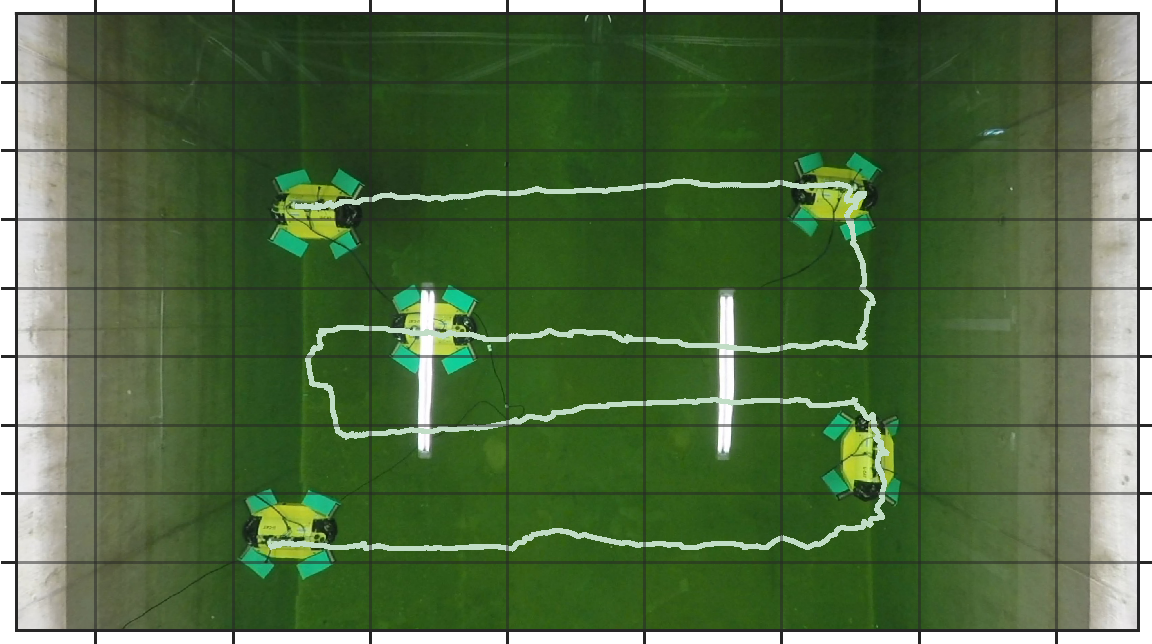
\includegraphics[width=3.0in]{img/autodepthtrajectory/autodepth.pdf}
\caption{Lawnmower trajectory with automatic depth control.}
\label{autodepthtrajectory}
\end{figure}



\section{Discussion}
We discuss the possible use-cases for different control approaches. We also describe how we are going to extend the work. We will include the absolute position measurements from hydrophone array and modem-based LBL into EKF to reduce the error in position measurement. Also sonar array for obstacle avoidance. 


\section{Conclusion}
Contribution:
\begin{itemize}
	\item Novel type of assisted control scheme for four-flipper robots using weighted control.
	\item Demonstration that the control scheme can also be extended for fully-autonomous control.
	\item Characterization of different control schemes and evaluation of their usability for different inspection tasks.
\end{itemize}

\section*{Acknowledgment}


The authors would like to thank...

\bibliographystyle{IEEEtran}
\bibliography{IEEEabrv,references}

\end{document}


